\documentclass[11pt,a4paper]{report}
%\documentclass[12pt,a4paper]{article}

\usepackage{bm}
\usepackage{amssymb}
\usepackage{amsfonts}

\usepackage{notebook2e}
\usepackage{wrisym}

\usepackage{amsmath}

%\usepackage{epsfig}
%\usepackage{german}
%%For list of figures and list of tables in table of contents to work
\usepackage[nottoc]{tocbibind}
\usepackage{wp2latex}
\usepackage{InputPS}
\usepackage{graphics}
\usepackage{latexsym}
\usepackage{braket}
\usepackage{tabls}
\usepackage[mathscr]{eucal}
%\usepackage{pst-fill}
%\usepackage{pstcol} 
\usepackage{color}
\usepackage{here}
\usepackage{longtable}
\usepackage{array}
\usepackage{caption2}
\usepackage{eqnarray}
\usepackage{sectsty}
\usepackage{fancyhdr}
\usepackage{fancybox}
%\usepackage{colortbl}
%\usepackage{colortab}
%\usepackage{a4wide}
\usepackage{framed}
% Postscript fonts
%\usepackage{courier}
%\usepackage[T1]{fontenc}
%\usepackage{textcomp}
\usepackage{cite}
\usepackage{feynarts}
%\usepackage{draftcopy}

\definecolor{gray}{gray}{.5}
\definecolor{lightgray}{gray}{.85}
\definecolor{steelblue}{rgb}{0.153, 0.102, 0.255}
\definecolor{lightblue}{rgb}{0,0.2,0.5}

\def\xstrut{\raisebox{-1.9ex}{\rule{0pt}{5ex}}}

\def\overscript#1#2{\mathop{#2}\limits^{{}_{\:#1}}\!{}}

%% Conditionals in TeX
\usepackage{ifthen}

% Text width and height
\newcommand{\twt}{490pt}
\newcommand{\tht}{540pt}
% Text margins
\newcommand{\lmargn}{-12pt}
\newcommand{\rmargn}{0pt}
% Two-column widths
\newcommand{\tmlwidth}{122pt}
\newcommand{\tmrwidth}{220pt}
\newcommand{\dbskip}{-73pt}

\setlength{\textwidth}{\twt}
%\setlength{\textheight}{\tht}

%%%%%%%%%%%%%%%%%%%%%%%%%%%%%%%%%%%%%%%%%%%%%%%%%%%%%%%%%%%%%%%%
% Mathematica boxes in two column environment
%%%%%%%%%%%%%%%%%%%%%%%%%%%%%%%%%%%%%%%%%%%%%%%%%%%%%%%%%%%%%%%%

\makeatletter
\long\def\dispSFinM{\@ifnextchar[{\dodispSFinM}{\dodispSFinM[n]}}
\makeatother

\long\def\dodispSFinM[#1]#2{%%
    %\vskip-\lastskip 
    %\if #1p
    %    \vskip \aboveinskip %
    %\else
    %    \vskip\aboveinskip\global\matharrayfalse
    %    \global\setbox\Minbox=\vbox
    %\fi
    {\parindent 0pt\mathfontsize%
    \if #1p
        \def\@writabarray{\@ifnextchar[{\@wriarray}{\@wriarray[p]}}
    \else
        \def\@writabarray{\@ifnextchar[{\@wriarray}{\@wriarray[t]}}
        \def\@tabarray{\@ifnextchar[{\@array}{\@array[t]}}
    \fi
    \def\MathBegin##1{\global\matharraytrue%
        \kern -\arraycolsep\def\tempa{\csname ##1\endcsname}\tempa}
    \ifinprompt\global\advance\promptcount by 1%
            \leavevmode\kern\mathindent\In{\INPROMPT\ \relax}%
    \else\ifprompt%
            \global\advance\promptcount by 1%
            \leavevmode%
            \ifpromptbreak%
                    \kern\mathindent\In{In[\the\promptcount]:= }\break
                    \bgroup\mbox{}\kern\mathindent\kern 12pt
            \else\kern\mathindent\In{In[\the\promptcount]:= }%
            \fi%
        \else%
            \leavevmode\mbox{}\kern\mathindent%
    \fi\fi%
    \def\Mvariable##1{\mathrm{##1}}%
    \mathversion{monobold}\fixttmath\ttfamily\bfseries$\displaystyle
    %\lefthyphenmin=100
    %\righthyphenmin=100
    \parbox[t]{\tmrwidth}{#2}$%
    \ifprompt\else\ifshowprompts\global\prompttrue\fi\fi%
    \global\inpromptfalse\global\promptbreakfalse}%
    %\if #1p\relax\else\copy\Minbox\fi%
    {\ifmatharray\advance\belowinskip 3pt\global\matharrayfalse\fi%
    \vskip\belowinskip}}

\makeatletter
\long\def\dispSFoutM{\@ifnextchar[{\dodispSFoutM}{\dodispSFoutM[n]}}
\makeatother

\long\def\dodispSFoutM[#1]#2{%%
    \vskip-\lastskip\vskip\aboveoutskip%
    \global\setbox\Moutbox=\vbox
    {\parindent 0pt\mathfontsize%
    \if #1p
        \def\@writabarray{\@ifnextchar[{\@wriarray}{\@wriarray[p]}}
    \else
        \def\@writabarray{\@ifnextchar[{\@wriarray}{\@wriarray[t]}}
        \def\@tabarray{\@ifnextchar[{\@array}{\@array[t]}}
    \fi
    \def\MathBegin##1{\global\matharraytrue%
        \kern -\arraycolsep\def\tempa{\csname ##1\endcsname}\tempa}
    \ifoutprompt%
            \leavevmode\kern\mathindent\Out{\OUTPROMPT\ \relax}%
    \else\ifprompt%
            \leavevmode%
            \ifpromptbreak%
                    \kern\mathindent\Out{Out[\the\promptcount]= \relax}\break
                    \bgroup\mbox{}\kern\mathindent\kern 12pt
            \else\kern\mathindent\Out{Out[\the\promptcount]= \relax}%
            \fi%
        \else%
            \leavevmode\mbox{}\kern\mathindent%
    \fi\fi%
    \def\Mvariable##1{\mathrm{##1}}%
    \mathversion{mono}\fixttmath\ttfamily$
    \displaystyle \parbox[t]{\tmrwidth}{\hspace*{-4pt}#2}$%
    \ifprompt\else\ifshowprompts\global\prompttrue\fi\fi%
    \global\outpromptfalse\global\promptbreakfalse}%
    \if #1p\relax\else\copy\Moutbox\fi%
    {\ifmatharray\advance\belowoutskip 3pt\global\matharrayfalse\fi%
    \vskip\belowoutskip}}

\makeatletter
\long\def\dispTFoutM{\@ifnextchar[{\dodispTFoutM}{\dodispTFoutM[n]}}
\makeatother

\long\def\dodispTFoutM[#1]#2{%%
    \vskip-\lastskip\vskip\aboveoutskip%
    \global\setbox\Moutbox=\vbox
    {\parindent 0pt\mathfontsize%
    \if #1p
        \def\@writabarray{\@ifnextchar[{\@wriarray}{\@wriarray[p]}}
    \else
        \def\@writabarray{\@ifnextchar[{\@wriarray}{\@wriarray[t]}}
        \def\@tabarray{\@ifnextchar[{\@array}{\@array[t]}}
    \fi
    \def\MathBegin##1{\global\matharraytrue%
        \kern -\arraycolsep\def\tempa{\csname ##1\endcsname}\tempa}
    \ifoutprompt%
            \leavevmode\kern\mathindent\Out{\OUTPROMPT\ \relax}%
    \else\ifprompt%
            \leavevmode%
            \ifpromptbreak%
                    \kern\mathindent\Out{Out[\the\promptcount]= \relax}\break
                    \bgroup\mbox{}\kern\mathindent\kern 12pt
            \else\kern\mathindent\Out{Out[\the\promptcount]= \relax}%
            \fi%
        \else%
            \leavevmode\mbox{}\kern\mathindent%
    \fi\fi%
    \def\Mvariable##1{\mathrm{##1}}%
    $\displaystyle \parbox[t]{\tmrwidth}{#2}$%
    \ifprompt\else\ifshowprompts\global\prompttrue\fi\fi%
    \global\outpromptfalse\global\promptbreakfalse}%
    \if #1p\relax\else\copy\Moutbox\fi\vskip\belowoutskip}

\def\PreserveBackslash#1{\let\temp=\\#1\let\\=\temp}

%%%%%%%%%%%%%%%%%%%%%%%%%%%%%%%%%%%%%%%%%%%%%%%%%%%%%%%%%%%%%%%%
% SWITCH FOR PDFLATEX or LATEX
%%%%%%%%%%%%%%%%%%%%%%%%%%%%%%%%%%%%%%%%%%%%%%%%%%%%%%%%%%%%%%%%

\ifx\pdfoutput\undefined
\def\pdf{0}
\else
\def\pdf{1}
\fi
\ifx\pdfoutput\relax
\def\pdf{0}
\else
\def\pdf{1}
\fi
%\ifthenelse{\pdf = 0}{
\ifthenelse{\pdf = 0 \or \isundefined{\pdfoutput}}{
%%%%%%%%%%%%%%%%%%%%%%%%%%%%%%%%%%%%%%%%% LATEX %%%
%%%
%%
%% Small caps for postscript
\usepackage{smallcap}
%% Provides \textsc
\usepackage{esscit}

%% Use these fonts if not converting to pdf (with ps2pdf)
%\newcommand{\mma}{{\scfamily\slshape Mathematica}\xspace}
%\newcommand{\fc}{{\scfamily\slshape FeynCalc}\xspace}
%\newcommand{\fa}{{\scfamily\slshape FeynArts}\xspace}
%\newcommand{\fctables}{{\scfamily\slshape fctables}\xspace}
%\newcommand{\fcloops}{{\scfamily\slshape fcloops}\xspace}
%\newcommand{\fctools}{{\scfamily\slshape fctools}\xspace}
%\newcommand{\general}{{\scfamily\slshape general}\xspace}
%\newcommand{\qcd}{{\scfamily\slshape qcd}\xspace}
%\newcommand{\fcdevel}{{\scfamily\slshape fcdevel}\xspace}
%\newcommand{\fphi}{{\scfamily\slshape PHI}\xspace}
%\newcommand{\tarcer}{{\scfamily\slshape TARCER}\xspace}
%\newcommand{\hip}{{\scfamily\slshape HIP}\xspace}
%\newcommand{\lpts}{{\scfamily\slshape LoopTools}\xspace}
%\newcommand{\FoF}{{\scfamily\slshape FormF}\xspace}
%\newcommand{\FF}{{\scfamily\slshape FF}\xspace}
%\newcommand{\defsc}{{\scfamily\slshape Italic small caps}\xspace}

%% When converting to pdf, the fancy fonts above get bitmapped; thus drop them
\newcommand{\mma}{Mathematica\xspace}
\newcommand{\fc}{FeynCalc\xspace}
\newcommand{\fa}{FeynArts\xspace}
\newcommand{\fctables}{fctables\xspace}
\newcommand{\fcloops}{fcloops\xspace}
\newcommand{\fctools}{fctools\xspace}
\newcommand{\general}{general\xspace}
\newcommand{\qcd}{qcd\xspace}
\newcommand{\fcdevel}{fcdevel\xspace}
\newcommand{\fphi}{PHI\xspace}
\newcommand{\tarcer}{TARCER\xspace}
\newcommand{\hip}{HIP\xspace}
\newcommand{\lpts}{LoopTools\xspace}
\newcommand{\FoF}{FormF\xspace}
\newcommand{\FF}{FF\xspace}
\newcommand{\defsc}{Italic small caps\xspace}

\usepackage[dvips]{graphicx}       %%% graphics for dvips
\DeclareGraphicsExtensions{.eps}   %%% standard extension for included graphics
%% Thumbnails in case of ps2pdf
%\usepackage[ps2pdf]{thumbpdf}
%% use dvips (or dvipdf or dvipdfm??) if converting on to pdf,
%% otherwise hypertex and then remember to run dvips -z
\usepackage[pdfstartview=FitH,pdffitwindow=true,bookmarks=true,bookmarksopen=true,bookmarksopenlevel=1,backref=page,pagebackref=false,
hyperfigures=false,colorlinks=true,linkcolor=lightblue,anchorcolor=lightblue,
citecolor=lightblue,filecolor=lightblue,menucolor=lightblue,pagecolor=lightblue,
urlcolor=lightblue,dvips,plainpages=false,hypertexnames=false]{hyperref}
%\usepackage[ps2pdf,                %%% hyper-references for ps2pdf
%bookmarks=true,%                   %%% generate bookmarks ...
%bookmarksnumbered=true,%           %%% ... with numbers
%hypertexnames=false,%              %%% needed for correct links to figures !!!
%breaklinks=true,%                  %%% breaks lines, but links are very small
%linkbordercolor={0 0 1},%          %%% blue frames around links
%pdfborder={0 0 112.0}]{hyperref}%  %%% border-width of frames 
%                                      will be multiplied with 0.009 by ps2pdf
%
\hypersetup{
pdfauthor = {Rolf Mertig and Frederik Orellana},
pdftitle = {FeynCalc 5.0 - A Guide for Quantum Field Theory practicioners},
pdfsubject = {Computational Particle Physics},
pdfkeywords = {Quantum Field Theory, Loops, Integrals, Feynman diagrams, Scattering, Kinematics},
pdfcreator  = {LaTeX with hyperref package},
pdfproducer = {dvips + ps2pdf}
}

%% Caption for gray boxes
\def\GrayCaption#1{\setbox0=\hbox{\footnotesize\sffamily #1}%
     \vspace{-15pt}
     \begin{flushleft}\leavevmode%
     \vbox{\hsize=\hsize\footnotesize\sffamily #1\par}\end{flushleft}
  }
}{
%%%
%%%%%%%%%%%%%%%%%%%%%%%%%%%%%%%%%%%%%%%%%%%%%%%%%%%%%%%%%% PDFLATEX %%%
%%%
%% Graphics for pdfLaTeX
\usepackage[pdftex]{graphicx}

%\setlength{\fboxrule}{0.0138889in}
%\setlength{\fboxsep}{0.8pt}

%% Thin frame around shaded boxes
%\makeatletter
%\renewenvironment{shaded}{%
%  \def\FrameCommand{
%  %\setlength{\fboxsep}{8pt}
%  \fcolorbox{gray}{shadecolor}}
%  \fram@d {}}
% {\endfram@d}
%\makeatother

\renewcommand{\graybox}[3]{
\definecolor{shadecolor}{gray}{#3}
%\fcolorbox{gray}{lightgray}{\parbox{\textwidth}{
\begin{shaded}
#1
\end{shaded}
}

%% Standard extension for included graphics
\DeclareGraphicsExtensions{.pdf}
\newcommand{\mma}{\fontfamily{pmnx}\selectfont\textit{Mathematica}\fontfamily{ptm}\selectfont\xspace}
\newcommand{\fc}{\fontfamily{pmnx}\selectfont\textit{FeynCalc}\fontfamily{ptm}\selectfont\xspace}
\newcommand{\fa}{\fontfamily{pmnx}\selectfont\textit{FeynArts}\fontfamily{ptm}\selectfont\xspace}
\newcommand{\fctables}{\fontfamily{pmnx}\selectfont\textit{fctables}\fontfamily{ptm}\selectfont\xspace}
\newcommand{\fcloops}{\fontfamily{pmnx}\selectfont\textit{fcloops}\fontfamily{ptm}\selectfont\xspace}
\newcommand{\fctools}{\fontfamily{pmnx}\selectfont\textit{fctools}\fontfamily{ptm}\selectfont\xspace}
\newcommand{\general}{\fontfamily{pmnx}\selectfont\textit{general}\fontfamily{ptm}\selectfont\xspace}
\newcommand{\qcd}{\fontfamily{pmnx}\selectfont\textit{qcd}\fontfamily{ptm}\selectfont\xspace}
\newcommand{\fcdevel}{\fontfamily{pmnx}\selectfont\textit{fcdevel}\fontfamily{ptm}\selectfont\xspace}
\newcommand{\fphi}{\fontfamily{pmnx}\selectfont\textit{PHI}\fontfamily{ptm}\selectfont\xspace}
\newcommand{\tarcer}{\fontfamily{pmnx}\selectfont\textit{TARCER}\fontfamily{ptm}\selectfont\xspace}
\newcommand{\hip}{\fontfamily{pmnx}\selectfont\textit{HIP}\fontfamily{ptm}\selectfont\xspace}
\newcommand{\lpts}{\fontfamily{pmnx}\selectfont\textit{LoopTools}\fontfamily{ptm}\selectfont\xspace}
\newcommand{\FoF}{\fontfamily{pmnx}\selectfont\textit{FormF}\fontfamily{ptm}\selectfont\xspace}
\newcommand{\FF}{\fontfamily{pmnx}\selectfont\textit{FF}\fontfamily{ptm}\selectfont\xspace}
\newcommand{\defsc}{\fontfamily{pmnx}\selectfont\textit{Italic small caps}\fontfamily{ptm}\selectfont\xspace}
%% Thumbnails in case of pdfLaTeX
%\usepackage[pdftex]{thumbpdf}
%% Hyper-references for pdflatex
\usepackage[pdfstartview=FitH,pdffitwindow=true,bookmarks=true,bookmarksopen=true,
bookmarksopenlevel=5,backref=page,pagebackref=false,
hyperfigures=false,colorlinks=true,linkcolor=lightblue,anchorcolor=lightblue,
citecolor=lightblue,filecolor=lightblue,menucolor=lightblue,pagecolor=lightblue,
urlcolor=lightblue,pdftex,plainpages=false,hypertexnames=false]{hyperref}
%\usepackage[pdftex,
%bookmarks=true,%                   %%% generate bookmarks ...
%bookmarksnumbered=true,%           %%% ... with numbers
%hypertexnames=false,%              %%% needed for correct links to figures !!!
%breaklinks=true,%                  %%% break links if exceeding a single line
%linkbordercolor={0 0 1}]{hyperref} %%% blue frames around links
%                                  %%% pdfborder={0 0 1} is the default
%% Graphics for pdfLaTeX
\hypersetup{
pdfauthor = {Rolf Mertig and Frederik Orellana},
pdftitle = {Guide to FeynCalc},
pdfsubject = {Computational Particle Physics},
pdfkeywords = {Loops, Integrals, Feynman diagrams, Amplitudes, Scattering, Kinematics},
%pdfcreator = {LaTeX with hyperref package},
%pdfproducer = {dvips + ps2pdf}
%pdfproducer = {pdflatex}
}
%                                  %%% pdfcreator, pdfproducer, 
%                                      and CreatioDate are automatically set
%                                      by pdflatex !!!
%% Force LaTeX-like character spacing
\pdfadjustspacing=1
%
%% Caption for gray boxes
\def\GrayCaption#1{\setbox0=\hbox{\footnotesize\sffamily #1}%
     \vspace{-5pt}
     \begin{flushleft}\leavevmode%
     \vbox{\hsize=\hsize\footnotesize\sffamily #1\par}\end{flushleft}
  }
}
%%%%%%%%%%%%%%%%%%%%%%%%%%%%%%%%%%%%%%%%%%%%%%%%%%% END OF CONDITION %%%

%%%%%%%%%%%%%%%%%%%%%%%%%%%%%%%%%%%%%%%%%%%%%%%%%%%%%%%%%%%%%%%%
\begin{document}
%%%%%%%%%%%%%%%%%%%%%%%%%%%%%%%%%%%%%%%%%%%%%%%%%%%%%%%%%%%%%%%%

%%%%%%%%%%%%%%%%%%%%%%%%%%%%%%%%%%%%%%%%%%%%%%%%%%%%%%%%%%%%%%%%
% Abbreviations
%%%%%%%%%%%%%%%%%%%%%%%%%%%%%%%%%%%%%%%%%%%%%%%%%%%%%%%%%%%%%%%%

\newcommand{\tr}{{\rm Tr}}
\newcommand{\intd}{{\rm d}}
\def\re{{\rm Re}}
\def\im{{\rm Im}}

%% Directory with images
\newcommand{\FigDir}{Figures}
\newcommand{\mindent}{\hspace*{12pt}}
\newcommand{\mb}[1]{{\small\tt \textbf{#1}}}

\newcommand{\disp}{\displaystyle}
\newcommand{\es}{\varepsilon \hspace{-0.5em}/\hspace{0.1em}}                   
\newcommand{\ra}{ $\, \rightarrow \,$ }
\newcommand{\as}{ a \hspace{-1.5mm} /}
\newcommand{\bs}{ b \hspace{-1.5mm} /}
\newcommand{\cs}{ c \hspace{-1.5mm} /}
\newcommand{\ds}{ d \hspace{-1.5mm} /}
\newcommand{\ks}{ k \hspace{-1.5mm} /}
\newcommand{\ps}{ p \hspace{-1.3mm} /}
\newcommand{\bps}{ p \hspace{-1.5mm} /}
\newcommand{\qs}{ q \hspace{-1.2mm} /}
\newcommand{\bqs}{ q \hspace{-1.6mm} /}

\newcommand{\op}[1]{{\it #1}}
\newcommand{\phat}{\^\,\hspace{-2pt}}
%% Normal font size in sub- and superscripts
\newcommand{\blineskip}{12pt}
\newcommand{\clineskip}{20pt}
\newcommand{\subscript}[2]{\setlength{\baselineskip}{\clineskip}${\displaystyle #1}_{\hspace*{2pt}\substack{\vspace*{4pt}\\ \displaystyle #2}}$}
\newcommand{\superscript}[2]{\setlength{\baselineskip}{\clineskip}${\displaystyle #1}^{\hspace*{0pt}\substack{\displaystyle #2\\ \vspace*{0pt}}}$}
\newcommand{\Superscript}[2]{\setlength{\baselineskip}{\clineskip}#1^{\displaystyle #2}}
\newcommand{\Subscript}[2]{\setlength{\baselineskip}{\clineskip}#1_{\displaystyle #2}}
%% Normal font size in fractions
\newcommand{\Frac}[2]{\setlength{\baselineskip}{\clineskip}$\frac{\substack{\displaystyle #1\\ \hspace*{2pt}}}{\substack{\hspace*{4pt}\\ \displaystyle #2}}$}
\newcommand{\frc}[2]{\setlength{\baselineskip}{\clineskip}\frac{\displaystyle #1}{\displaystyle #2}}

\newcommand\bksl{\char '134 }   % A backslash character for \tt font
%\newcommand{\lb}{\char '173 } % A left brace character for \tt font
%\newcommand{\rb}{\char '175 } % A right brace character for \tt font

%%%%%%%%%%%%%%%%%%%%%%%%%%%%%%%%%%%%%%%%%%%%%%%%%%%%%%%%%%%%%%%%
% Layout definitions
%%%%%%%%%%%%%%%%%%%%%%%%%%%%%%%%%%%%%%%%%%%%%%%%%%%%%%%%%%%%%%%%

%% Control the paragraph indentation
\setlength{\parindent}{0pt}
%% Add space between paragraphs
\setlength{\parskip}{3pt}

\setcounter{tocdepth}{2}
%% Add space between lines in equation arrays
\setlength{\extrarowheight}{0pt}
\renewcommand{\arraystretch}{1.4}
%\setlength\tablinesep{10pt}
%\setlength\arraylinesep{10pt}
%\setlength\extrarulesep{10pt}

\setlength{\arrayrulewidth}{0.1pt}
\newcommand{\hhline}{\hline \\}

%% Definition boxes

\newcommand{\otabtwo}[2]{
\begin{table}[H]
\graybox{
%Change RM 11 Sept 2003
%\begin{longtable}{p{0.42\textwidth ~~~~~~~} >{\flushleft\vspace*{-13.2pt}}p{0.50\textwidth ~~~~~~~}}
% These numbers were chosen (after a lot of trials) to have some alignment
% of \otabtwo, \otabthree and \domtog.
% Typographically it just looks better, and is less tiresome for the eyes.
% B.t.w. this also seems to have been the point with the layout of the old FeynCalc guide.
\begin{longtable}{p{0.32\textwidth ~~~~~~~} >{\flushleft\vspace*{-13.2pt}}p{0.55\textwidth ~~~~~~~}}
#1
\end{longtable}
}{.3}{.95}
\GrayCaption{#2}
\end{table}\setlength{\baselineskip}{\blineskip}
}

\newcommand{\otabthree}[2]{\renewcommand{\arraystretch}{1.0}
\begin{table}[H]
\graybox{
\begin{longtable}{p{0.25\textwidth} p{0.2\textwidth} p{0.45\textwidth}}
#1
\end{longtable}
}{.3}{.95}
\GrayCaption{#2}
\end{table}\renewcommand{\arraystretch}{1.4}\setlength{\baselineskip}{\blineskip}
}

\newcommand{\mbs}[1]{\raggedleft{\mb{#1}}}

%\newcommand{\beom}{\begin{longtable}{rl@{~-~}p{\textwidth}}}
\newcommand{\beom}{\begin{longtable}{p{\tmlwidth} p{\tmrwidth}}}
%\newcommand{\beom}{\begin{longtable}{l@{\extracolsep{\fill}} l@{\extracolsep{\fill}}}}

\newcommand{\enom}{\end{longtable}}

\newcommand{\domtog}[3]{
\setlength{\leftskip}{\dbskip}
\setlength{\rightskip}{0pt}
\begin{parbox}[t]{\tmlwidth}{\PreserveBackslash\raggedright
\footnotesize\noindent \hspace{-6pt} #3
}

\end{parbox} &
\begin{parbox}[t]{\tmrwidth}{
\setlength{\leftskip}{-53pt}
\footnotesize
\begin{CellGroup}
\dispSFinM{#1}
\vspace*{4pt}
\dispTFoutM{#2}
\end{CellGroup}}
\end{parbox}\\
}

\newcommand{\dtog}[3]{
\setlength{\leftskip}{\dbskip}
\setlength{\rightskip}{0pt}
\begin{parbox}[t]{\tmlwidth}{\PreserveBackslash\raggedright
\footnotesize\noindent \hspace{-6pt} #3}
\end{parbox} &
\begin{parbox}[t]{\tmrwidth}{
\setlength{\leftskip}{-53pt}
\footnotesize
\begin{CellGroup}
\dispSFinM{#1}
\end{CellGroup}}
\end{parbox}\\
}

\newcommand{\domptog}[4]{
\setlength{\leftskip}{\dbskip}
\setlength{\rightskip}{0pt}
\begin{parbox}[t]{\tmlwidth}{\PreserveBackslash\raggedright
\footnotesize\noindent \hspace{-6pt} #3}
\end{parbox} &
\begin{parbox}[t]{\tmrwidth}{
\setlength{\leftskip}{-53pt}
\footnotesize
\begin{CellGroup}
\dispSFinM{#1}
\texttt{#4}
\vspace*{4pt}
\dispTFoutM{#2}
\end{CellGroup}}
\end{parbox}\\
}

%% Mathematica code
\newcommand{\len}{0pt}
\newcommand{\ind}{\leftskip \len}
\newcommand{\mcode}[1]{
\parbox{0.8\textwidth}{
\setlength{\leftskip}{\len}
\mb{\textbf{ \\ #1 \\ }}
}
}

\renewcommand{\thesection}{\arabic{section}}
\renewcommand{\thechapter}{\arabic{chapter}}

% Sans serif font for chapter, section, etc.
\allsectionsfont{\sffamily}
\subsectionfont{\huge \sffamily}

% Reference section definitions

\newcommand{\fname}[1]{
  $\blacksquare$ \ \ {\large\mb{#1}}
  \begin{quote}
}
\newcommand{\fheading}[1]{
\setlength{\leftskip}{4pt}
}
\newcommand{\fusage}[1]{#1\vspace*{10pt}\newline}
\newcommand{\fnotes}[1]{
\setlength{\parindent}{0pt}
\setlength{\parskip}{0pt}
#1}
\newcommand{\ftabtwo}[1]{
\begin{longtable}[H]{p{0.3\textwidth} p{0.54\textwidth
}}
#1
\end{longtable}
}
\newcommand{\ftabthree}[1]{
%\begin{longtable}[H]{p{0.2\textwidth} p{0.24\textwidth} p{0.4\textwidth}}
%\renewcommand{\leftsk}{\leftskip}
\renewcommand{\arraystretch}{0.8}
\renewcommand{\arraycolsep}{0}
\begin{longtable}[H]{p{0.23\textwidth} p{0.1\textwidth} p{0.5\textwidth}}
#1
\end{longtable}
%\setlength{\leftskip}{\leftsk}
}
\newcommand{\seepage}{}
\newcommand{\ffinish}{\end{quote}}

%%%%%%%%%%%%%%%%%%%%%%%%%%%%%%%%%%%%%%%%%%%%%%%%%%%%%%%%%%%%%%%%
% Document
%%%%%%%%%%%%%%%%%%%%%%%%%%%%%%%%%%%%%%%%%%%%%%%%%%%%%%%%%%%%%%%%

\title{\raggedright \hspace*{1pt} {\bf ***DRAFT***} \\
\vspace*{12pt}
{\LARGE FeynCalc 5.0}\\
\vspace*{40pt}
{\Large A Guide for Quantum Field Theory practitioners}}
\author{\hspace*{-10pt}
\parbox{\textwidth}{\raggedright Rolf Mertig \\
and \\
Frederik Orellana}}
%\date{\hspace*{4pt} \parbox{\textwidth}{\raggedright CERN\\ September 12th, 2003}}
\date{}
{\sffamily
\maketitle
}

\pagenumbering{Roman}

\newpage
%\phantomsection
%\addcontentsline{toc}{section}{Contents}
%\thispagestyle{empty}    % No page number on contents page
\tableofcontents
%\clearpage
\newpage

\pagenumbering{roman}
%\pagenumpos{\pnbc}
\setcounter{page}{1}
% Headings on each page
\pagestyle{fancy}    % Go for customized headings

\setlength{\textwidth}{\twt}
\setlength{\textheight}{\tht}
\oddsidemargin \lmargn
\evensidemargin \rmargn

\setcaptionwidth{\textwidth}

\lhead{\nouppercase{\it \rightmark}}
\chead{}
\rhead{\thepage}
\fancyfoot[C]{}

%% Deal with overfull vbox warnings
%\addtolength{\headheight}{12pt}
%\addtolength{\footskip}{12pt}

\sectionmark{Preface}
\section*{Preface}

This book is for practitioners of calculations in perturbative QCD,
the Standard Model, Chiral Perturbation Theory and other theories.
The intention is to serve both educational as well as research purposes.
This is reflected in the layout of the parts.
The first part is a tutorial-like introduction with many small examples.
It is necessarily of a rather technical character and should prepare the
reader for doing real physics calculations.
The second part contains a variety of example calculations from textbook
%to research level. The interested student will find here calculations calculations
to research level. The interested student will find here calculations 
from the literature worked through in a detail not found elsewhere.
The researcher will find calculations that should provide a starting point
for calculations of his or her own research.
The third part is a reference guide, listing all important functions,
also with many small examples.
%The user is assumed to know Quantum Field Theory and have some understanding of \mma.
%It is strongly recommended to study the \mma book \cite{Mathematica} by
%Stephen Wolfram before starting with \fc.

Over the years, the detailed course of and motivation for the development of \fc has
changed somewhat both in scope and focus. The reasons are the different research
interests of the two authors, the relative slowness of \mma and the rapid development of
multi-loop calculations carried out with FORM and programs based on FORM 
\cite{Vermaseren:2000nd, Hahn:1998yk}, which are  more suited for very large scale calculations.
Also \fc has tools to interact with FORM. This is particularly useful if the CPU time is
an issue or if truly large expressions occur and a very efficient way to handle those 
expressions is needed. FORM is very much suited for this task. 
On the other hand, general purpose computer algebra systems like \mma have more flexibility in their user interface and one can use the already provided libraries for operations like
integration and series expansions and more mathematical tasks.
%3) the rapid development of the raw computing power of hardware. 
%As a consequence the focus has moved away from providing cutting edge results of multi-loop
%calculations in the Standard Model and in QCD. 
One focus has been to explore other types of calculations than the evaluation of Feynman
diagrams, e.g. complex algebraic manipulations of quantum fields and lagrangians, traditionally done by hand only.
Such calculations have become feasible because of the steep increase of the computing
power of commodity hardware.

Despite the motivations driving development, the central vision remains largely the same: 
\fc was conceived as and continues to be developed as a general-purpose, relatively easy to use,
modular toolbox for quantum field theory calculations. 
Dirac algebra utilities, Lorentz and Color algebra manipulation capabilities, 
functional derivation utilities, integral and other tables have been cleanly 
separated off in distinct functions which 
do well-defined operations.
Such basic functions can then be used  on a higher level to build sophisticated model dependent functions.

In the following we list what we consider the most important general principles that the \fc
project strives to promote:
%%SOFAR

\begin{itemize}

%
%\item{{\bf Standardization.} In order to reuse code, clear standards should be formulated,
%thoroughly documented and followed. The aim should be to reach common standards with
%other similar or related projects (using other programming languages) for fields, lagrangians,
%Lorentz-vectors, etc. in the end allowing easy comparison of calculations of the same process.}

\item{{\bf Systematic knowledge build-up.} In physics calculations, errors due to typos or
other trivial mistakes are not acceptable, therefore the code used should be as thoroughly
checked as possible by as many people as possible. This implies openness and adherence to
standards. It is proposed to build up a repository of lagrangians, amplitudes and integrals,
stored in a standardized electronic form.}

%\item{{\bf Algorithm optimization.} The more people using (an implementation of) an algorithm,
%the better the chances of improving (the implementation of) it.}

\item{{\bf Fast prototyping.} Quickly trying out new quantum field theory models should be made
easier by using the building blocks provided by a clear standardization as well as a set of
functions for the most common calculational tasks.}

\item{{\bf Checks.} Calculations should, when possible, be performed by different methods.
Thus, \fc should be used to check hand calculations or the results of other programs and
vice versa.}

\end{itemize}

%Notice in this connection that the standards put forth in this document (and in the code) are what
%the authors consider to be the most general but still useful standards for doing quantum fields
%theory with \mma. This means that standards are to be considered as relatively fixed, but not that
%they cannot be changed, given good enough reasons.

From all of the above it should be clear that we consider interaction with users to be crucial
for the further evolving of \fc. Therefore, suggestions and in particular
code contributions are warmly welcomed. Smaller contributions can be contributed
on the web site \href{http://www.feyncalc.org/}{http://www.feyncalc.org/}; 
larger contributions should be coordinated with the developers.
Though much testing of the code has been done, there is absolutely no claim that
\fc is bug-free. You should be sceptical about the results, and when you are sure the
program  returns a wrong answer, you are encouraged to report it via the web site
\href{http://www.feyncalc.org/}{http://www.feyncalc.org/}.

\subsection*{Version History}

The roots of \fc go back to 1987. 
During a stay as a graduate student in Albuquerque, New Mexico, Rolf Mertig learned to program in Macsyma \cite{Drinkard:1981dr} from the experts Stanly Steinberg and Michael Wester. Back to Germany, 
elementary particle physicists needed automation of the calculation of Feynman diagrams of eletroweak 
processes to one loop. The algorithms were partially developed together with 
Ansgar Denner and Manfred B\ODoubleDot{}hm and implemented in a 
purely functional way by Rolf Mertig during the years 1987 - 1989. 

The basic idea was to have general functions for some of the more mechanical parts of the diagram calculations, generalizable tools for use in calculations of different 1-loop processes, especially 1\(\rightarrow \)2 and 2\(\rightarrow \)2 processes. These included tools for:

\begin{itemize}

\item{Lorentz algebra.
\({g^{\Mvariable{\mu \nu }}}\multsp {p_{\mu }}
\multsp \rightarrow \multsp {p^{\nu }}
\multsp ,\multsp \multsp\)
\({g^{\Mvariable{\alpha \beta }}}{g_{\Mvariable{\alpha \beta }}}
   \multsp \rightarrow \multsp D\multsp \cdots\),}

\item{Dirac algebra.
\({{\gamma }^{\alpha }}\multsp {{\gamma }^{\nu }}
{{\gamma }_{\alpha }}\multsp \rightarrow \multsp 
(2-n)\multsp {{\gamma }^{\nu }},\multsp \multsp \)
\(\overvar{v}{\_}(p,m)\multsp 
\bps\)  \(\rightarrow \) - m \(\overvar{v}{\_}(p,m)\multsp \cdots\),}

\item{Passarino-Veltman tensor integral decomposition.
Applications of these tools included complete 1-loop processes in the Standard Model,
\({e^+}{e^-}\multsp \rightarrow 
\multsp Z\multsp H\multsp \),  \(\multsp {e^+}{e^-}\multsp \rightarrow \)
\(\multsp {W^+}{W^-}\multsp \)
and the 2-loop photon self-energy in QED.}

\end{itemize}

However, at the end of 1989 several problems showed up with the Macsyma implementation. The purely functional programming style proved to be difficult to debug and, in fact, inappropriate. The rudimentary pattern matcher in Macsyma was not useful. There was no way to incorporate new functions easily into the whole Macsyma system, and no possibility of providing online documentation. Furthermore, Macsyma's memory managment ("garbage collection") was slow when handling large expressions.

In early 1990 it became clear that \mma was a much more natural programming environment for \fc.

\subsubsection*{1990-1991 : The first version  of \fc in \mma}

In 1990, user-friendly  packages were built with extended automatic capabilities (\mb{OneLoop}, \mb{OneLoopSum}), and SU(3) algebra capabilities were added (\mb{SU3Simplify}).

In 1991 initial documentation was written and the program was made available on anonymous ftp-servers: mathsource.wolfram.com and canc.can.nl.

Applications from 1990 - 1996  included:

\begin{itemize}

\item 1-loop 2 \(\rightarrow \)2 processes in the Standard
Model, such as:

\({\rm gg}\multsp \rightarrow \multsp 
{\rm t \overline{t}} \multsp , \multsp \multsp
{{\rm e}^+}{{\rm e}^-}\multsp \rightarrow \multsp {\rm Z}\multsp {\rm H}\multsp, \multsp \multsp
%{{\rm W}^+}{{\rm W}^-}\multsp \)\(\rightarrow \) \({{\rm W}^+}{{\rm W}^-}\multsp, \multsp \multsp
{\rm gg} \rightarrow {\rm t\bar{t}} \),

\item background field gauge calculations,

\item high-energy approximation of \(\multsp{{\rm e}^+}
{{\rm e}^-}\multsp \rightarrow \multsp {{\rm W}^+}{{\rm W}^-}\multsp \),

\item  2-loop Standard Model self-energies.

\end{itemize}

No real attempt was made to provide tools for tree-level calculations. 
For this purpose other programs appeared, among them another  \mma package, \hip \cite{yeh}, developed at SLAC, 
CompHEP \cite{Pukhov:1999gg}, and of course FORM \cite{Vermaseren:2000nd}.

\subsubsection*{1992-1995 : \fc 2.0-2.2, unification and simplification.}

During this period of development the SU(3) algebra was changed to SU($N$). Several tools for automatic tree-level calculation were added, for example the function \mb{SquareAmplitude}. (Unfortunately, the  documentation was not updated.) All sub-packages were put into one file \(\big(\simeq {{10}^4}\) lines), "FeynCalc2.2beta.m" \footnote{This file is still available upon request}.

\subsubsection*{1993-1996 : \fc 3.0, modularization, typesetting, Operator Product Expansion (OPE)}

Due to the rapidly increasing amount of code, \fc was reorganized in a modular way. The definitions of each function are contained in a package file which is loaded only on demand. For the maintenance of hundreds of packages, totalling 2.5 megabytes, software engineering was needed.

\begin{itemize}

\item
In these years many improvements were made to the code, driven by the work of the author (Rolf Mertig) 
together with Willy van Neerven in perturbative Quantum Chromo Dynamics (QCD).

One effort was to build data bases: Convolutions, integrals, tensor integral transformation
formulae, Feynman rules,
and Feynman parameterizations. 
Applications include 2-loop spin-independent and spin-dependent Altarelli-Parisi splitting
functions \cite{Altarelli:1977zs}.

\item The new typesetting capabilities of \mma 3 (TraditionalForm) were used to substantially
improve the look of the output.
Typesetting rules were added for e.g. \({\overvar{\partial }{\rightarrow}}_{\mu } \multsp \).

\item Code was written to allow new abstract data types, for example for noncommutative algebra
 and for special integrals.

\item QCD tools for the Operator Product Expansion  (OPE)
were added.

\item Automatic Feynman rule derivation (with functional
differentation) was implemented in order to get special Feynman rules
for twist-2 (and higher) operators.

\end{itemize}

\subsubsection*{1997-2000 : \fc 4.0-4.1, QCD and OPE, ChPT, tables}

Another was the package \tarcer, which was initially an independent project, but then integrated
into \fc.  \tarcer \cite{Mertig:1998vk} adds two-loop functionality for propagator-type integrals
using the recurrence relations of Tarasov \cite{Tarasov:1997kx}.

In 2000 maintenance of the package was taken over by Frederik Orellana.
He worked in Chiral Perturbation Theory \cite{Gasser:1984gg} (ChPT) and made some changes, as well
as adding code to \fc in order to support ChPT and effective theories in general, and interfacing
with \fa. Also, first implementations of the 'tHooft-Veltman formulae \cite{'tHooft:1978xw} for
numerical evaluation of the one-loop integrals $B_0, C_0$ and $D_0$ were added. 

\pagenumbering{arabic}
%\pagenumpos{\pnbc}
\setcounter{page}{1}
\section{Introduction}

\fc is a ($\ge 3$) collection of utilities for algebraic calculations in 
high energy physics. It is implemented as a \mma package; that is,
a number of extensions to the programming language \mma,
themselves written in \mma. In the section below are described some of the main new
capabilities provided.

This document is the technical manual of \fc; explanations are sometimes rather short.
The user is assumed to know Quantum Field Theory and \mma.
It is strongly recommended to study the \mma book \cite{Mathematica} by
Stephen Wolfram before starting with \fc.

The original idea of \fc was to provide convenient tools 
for radiative corrections in the Standard Model of particle physics. 
The input for \fc, the analytical expressions for the diagrams, can be 
entered by hand or can be taken directly from the output of another 
package, \fa\ \cite{feynarts} .
The user can provide certain additional  information about the process 
under consideration, i.e. the kinematics and the choice of the standard 
matrix elements may be defined. Once this is done, \fc performs the 
algebraic calculations like tensor algebra, tensor integral decomposition and reduction,
yielding a polynomial in standard matrix elements,  special functions, kinematical 
variables and scalars.

\fc also provides calculator-type like features. You enter a Dirac trace 
in a very similar notation you use by hand and get back an answer, suitable 
for further manipulation. These features include basic operations like contraction of
tensors, simplification of products of Dirac matrices and trace calculation.

More complex algebraic operations have also been implemented, notably derivation
of polynomials in quantum fields with respect to such fields.

Over the years, the detailed course of and motivation for the development of \fc has
changed somewhat both in scope and focus. This has several reasons: 1) the different research
interests of the two authors; 2) the relative slowness of \mma and the rapid development of
multi-loop calculations carried out with tools more suited for very large scale calculations;
3) the rapid development of the raw computing power of hardware. The first two points have had as consequence that the focus has moved away from providing cutting edge results of loop calculations
in the Standard Model and in QCD. The last point has had as consequence that it has been possible
to explore other types of calculations, namely complex algebraic manipulations of quantum fields
and lagrangians, traditionally done by hand only.

Despite the motivations driving development, the central vision remains largely the same: \fc was conceived as and continues to be developed as a general-purpose modular package for quantum field theory calculations. Dirac algebra utilities, functional derivation utilities, integral tables etc. have been clearly separated off in distinct functions which do well-defined operations.  Such basic functions can then be used  on a higher level to build sophisticated model dependent functions.

In the following we list what we consider the most important missions of the \fc project:

\begin{itemize}

\item{{\bf Code reuse.} In calculations as complex as quantum field theory calculations,
the code used should be thoroughly checked and reinventing the wheel for every calculation should be avoided.}

\item{{\bf Standardization.} In order to reuse code, clear standards should be formulated, thoroughly documented and followed. This should also make it easier to reach common standards with other similar or related projects (using other programming languages) for fields, lagrangians, 4-vectors, etc. in the end allowing easy comparison of calculations of the same process.}

\item{{\bf Repository of lagrangians, amplitudes and integrals.} The agreement on standards allows the creation of a database of quantum field theory results stored in a standardized electronic form. We encourage users of \fc to contribute back the results they obtain.}

\item{{\bf Algorithm optimization.} The more people using (an implementation of) an algorithm, the better the chances of improving (the implementation of) it.}

\item{{\bf Fast prototyping.} Quickly trying out new quantum field theory models should be made easier by using the building blocks provided by a clear standardization as well as a set of functions for the most common calculational tasks.}

\end{itemize}

Notice in this connection that the standards put forth
in this document are what we consider to be the most general but still useful standards
for doing quantum fields theory with \mma. This means that that standards are
to be considered as relatively fixed, but not that we are unwilling to change them
given sufficiently good arguments.

From all of the above it should be clear that we consider interaction with users to be crucial
for the further evolving of \fc. Therefore, suggestions and in particular
code contributions are warmly welcomed. Smaller contributions can be emailed to
feyncalc@feyncalc.org; larger contributions should be coordinated with the
developers who can be reached at the same email address.
Though much testing of the code has been done, there is absolutely no claim that
\fc is bug-free. You should be sceptical about the results, and when you are sure the
program  returned a wrong answer, you are encouraged to send email
to feyncalc@feyncalc.org.

\subsection{Version History}

The roots of \fc go back to 1987. During a stay as a graduate student in Albuquerque, New Mexico, Rolf Mertig learned to program in Macsyma \cite{Drinkard:1981dr} from the experts Stanly Steinberg and Michael Wester. Meanwhile in Germany, elementary particle physicists needed automation of the calculation of Feynman diagrams of eletro-weak processes to one loop. The algorithms were provided mostly by Ansgar Denner and Manfred B\ODoubleDot{}hm and implemented in a purely functional way by Rolf Mertig during the years 1987 - 1989. 

The basic idea was to have general functions for some of the more mechanical parts of the diagram calculations, generalizable tools for use in calculations of different 1-loop processes, especially 1\(\rightarrow \)2 and 2\(\rightarrow \)2 processes. These included tools for:

\begin{itemize}

\item{Lorentz algebra.
\({g^{\Mvariable{\mu \nu }}}\multsp {p_{\mu }}
\multsp \rightarrow \multsp {p^{\nu }}
\multsp ,\multsp \multsp\)
\({g^{\Mvariable{\alpha \beta }}}{g_{\Mvariable{\alpha \beta }}}
   \multsp \rightarrow \multsp n\multsp \cdots\),}

\item{Dirac algebra.
\({{\gamma }^{\alpha }}\multsp {{\gamma }^{\nu }}
{{\gamma }_{\alpha }}\multsp \rightarrow \multsp 
(2-n)\multsp {{\gamma }^{\nu }},\multsp \multsp \)
\(\overvar{v}{\_}(p,m)\multsp 
\bps\)  \(\rightarrow \) - m \(\overvar{v}{\_}(p,m)\multsp \cdots\),}

\item{Passarino-Veltman - tensor integral decomposition.
Applications of these tools included complete 1-loop processes in the Standard Model,
\({e^+}{e^-}\multsp \rightarrow 
\multsp Z\multsp H\multsp \),  \(\multsp {e^+}{e^-}\multsp \rightarrow \)
\(\multsp {W^+}{W^-}\multsp \)
and the 2-loop photon self-energy in QED.}

\end{itemize}

However, at the end of 1989 several problems showed up with the Macsyma implementation. The purely functional programming style proved to be difficult to debug and, in fact, inappropriate. The rudimentary pattern matcher in Macsyma was not useful. There was no way to incorporate new functions easily into the whole Macsyma system, and no possibility of providing online documentation. Furthermore, Macsyma's memory managment ("garbage collection") was slow when handling large expressions.

In early 1990 it became clear that \mma was a much more natural (programming) environment for \fc.

\subsubsection*{1990-1991 : The first version  of \fc in \mma}

In 1990, user-friendly  packages were built with extended automatic capabilities (OneLoop, OneLoopSum), and SU(3) algebra capabilities
were added (SU3Simplify).

In 1991 initial documentation was written and the program was made available on anonymous ftp-servers: mathsource.wolfram.com and canc.can.nl

Applications from 1990 - 1996  included:

\begin{itemize}

\item 1-loop 2 \(\rightarrow \)2 processes in the Standard
Model, such as:

\({\rm gg}\multsp \rightarrow \multsp 
{\rm t \overline{t}} \multsp , \multsp \multsp
{{\rm e}^+}{{\rm e}^-}\multsp \rightarrow \multsp {\rm Z}\multsp {\rm H}\multsp, \multsp \multsp
{W^+}{W^-}\multsp \)\(\rightarrow \) \({{\rm W}^+}{{\rm W}^-}\multsp, \multsp \multsp
{\rm ZZ} \rightarrow {\rm ZZ} \)

\item background field gauge calculations,

\item High-energy approximation of \(\multsp{{\rm e}^+}
{{\rm e}^-}\multsp \rightarrow \multsp {{\rm W}^+}{{\rm W}^-}\multsp \).

\item  2-loop Standard Model self-energies.

\end{itemize}

No attempt was made to provide tools for tree-level calculations. For this purpose other programs appeared, among them another  \mma package, \hip \cite{yeh}, developed at SLAC.

\subsubsection*{1992-1995 : \fc 2.0-2.2, unification and simplification.}

During this period of development the SU(3) algebra was changed to SU($N$). Several tools for automatic tree-level calculation were added, for example the function \mb{SquareAmplitude}. (Unfortunately, the  documentation was not updated.) All sub-packages were put into one file \(\big(\simeq {{10}^4}\) lines). The result was FeynCalc2.2beta.m.

\subsubsection*{1993-1996 : \fc 3.0, modularization, typesetting}

Due to the rapidly increasing amount of code, \fc has been reorganized in a completely modular way. Each function in a package is a file which is loaded only on demand. For the maintenance of hundreds of packages, totalling 2.5 MegaByte, software engineering was needed.

\begin{itemize}

\item The new typesetting capabilities of \mma 3 (TraditionalForm) were used to substantially improve the look of the output. Typesetting rules were added for e.g., \({\overvar{\partial }{\rightarrow}}_{\mu } \multsp \).

\item Code was written to allow new abstract datatypes, for example for noncommutative algebra and for special integrals.

\item QCD tools for the Operator Product Expansion  (OPE)
were added.

\item Automatic Feynman rule derivation (with functional
differentation) was coded, in order to get special Feynman rules
for twist-2 (and higher) operators.

\end{itemize}

\subsubsection*{1997-2000 : \fc 4.0-4.1, QCD and OPE, ChPT, tables}

In these years Rolf Mertig made many improvements to the code, driven by his own work in perturbative Quantum Chromo Dynamics (QCD).

One effort was to build data bases: Convolutions, integrals, tensor integral transformation formulas, Feynman rules, and Feynman parameterizations. Applications include 2-loop spin-dependent and spin-independent Altarelli-Parisi Splitting functions.

Another was the package \tarcer, which was initially an independent project, but then integrated into \fc.  \tarcer \cite{Mertig:1998vk} adds two-loop functionality for propagator-type integrals using the recurrence relations of Tarasov \cite{Tarasov:1997kx}.

In 2000, maintanance of the package was taken over by Frederik Orellana. He worked in Chiral Perturbation Theory \cite{Gasser:1984gg} (ChPT) and made some changes, as well as adding code to \fc in order to support ChPT and effective theories in general, and interfacing with \fa. Also, a first implementation of the 'tHooft-Veltman formulae \cite{'tHooft:1978xw} for numerical evaluation of the one-loop integrals $B0, C0$ and $D0$ was added.

\subsection{Installation}

\begin{itemize}

\item{Download the file "HighEnergyPhysics-4.2.tar.gz" or "HighEnergyPhysics-4.2.zip" (if you're using using Windows you'll probably want the zip file).}

\item{Place the file in the directory "mathhome/AddOns/Applications", where "mathhome" is the directory containing your \mma installation. If you're on a Unix system, "mathhome" can also be "~/.Mathematica/x", where x is the version of your Mathematica installation. (if "~/.Mathematica/x/AddOns/Applications" does not exist, you can safely create it).}

\item{Make sure there is not already a directory "HighEnergyPhysics" (and move it out of the way if there is).}

\item{Unpack the file: Under UNIX, type {\tt tar -xvzf HighEnergyPhysics-4.2.tar.gz}; under Windows and MacOS, use some utility like WinZip or StuffIt Expander.}

\item{If you've made any customizations in the configuration file FCConfig.m, merge them from the file you've moved away into the new file.}

\item{Start Mathematica.}

\item{Choose 'Rebuild Help Index' from the 'Help' menu.}

\item Load \fc with \mb{<<HighEnergyPhysics`FeynCalc`}

\end{itemize}


\section{Input Functions}

The \fc syntax for metric tensors, four-vectors, Dirac matrices, etc.,
is such that the positioning of the arguments automatically defines the nature of the variables. %You can only enter algebraic objects; there
%is no possibility of working with explicit components of vectors
%or with specific Dirac matrices like $\gamma_0$ or $\gamma_2$.
No declaration of Lorentz indices or four-vectors has
to be made.
Covariant and contravariant Lorentz indices are treated on an equal basis,
assuming summation over (twice) repeated indices, where each pair of
indices are assumed to be co- and contravariant respectively.
Since explicit components of Lorentz tensors are not used, this
convention causes no problems.
The ambiguity in the sign of the Levi-Civita tensor can be
fixed by an option of the function \mb{DiracTrace} and
\mb{EpsChisholm}, see page \pageref{input}.

The input functions are macros that are immediately translated into
the internal representation of \fc. But these sometimes lengthy
internal representations are difficult to recognize when working
interactively. Therefore, some effort has been put into making the output
of \fc look as much as possible like typeset formulas.
The typesetting of \fc depends on the input/output interface in use.

\begin{itemize}
\item{\bf Terminal interface.} Per default \fc sets the global \mma variable
\mb{\$PrePrint} to \mb{FeynCalcForm},
forcing the display to be in a more readable manner.
It is important to realize that the display given by \mb{FeynCalcForm} is
different from the input syntax. Thus, you may not give as input,
for example, a scalar product in the result of a trace calculation
by copying the form you see on the screen. To have the output be the
internal representation, set \mb{\$PrePrint=.}. To return to formatted output,
set \mb{\$PrePrint = FeynCalcForm}.
\item{\bf Notebook interface.} \fc per default automatically sets the
\mma default output format type to \mb{TraditionalForm}. Because \fc defines
the \mb{TraditionalForm}-look of its objects, the output looks very much like
typeset formulas. Again, the screen output cannot be copied and used
as input. If the \mma default output format type
\footnote{The \mma default output format type is set using the
menu 'Cell' $\rightarrow$ 'Default Output Format Type'.}
is set to
%\mb{OutputForm},
\mb{InputForm} or \mb{StandardForm}, the
screen output is the internal representation of \fc and can be copied
and used as input. To obtain the same output as with a terminal interface,
set the \mma default output format type to \mb{OutputForm} and set
\mb{\$PrePrint = FeynCalcForm}. To return to formatted output, set
the \mma default output format type to \mb{TraditionalForm}.
\end{itemize}

In the rest of this guide the examples given will use the notebook interface.

The internal structure of \fc
is explained in section \ref{inside} and in the
reference section \ref{rg}. Usually it is not necessary to know it.
Notice simply that there are three layers of \fc: The input functions,
an output representation and the internal representation.

In order to do calculations in the framework of $D$-dimensional
regularization, \fc can be used for  calculations
in 4 or $D$
%or $D-4$
dimensions.
The dimension of  metric tensors, Dirac matrices and  four-vectors
is specified by setting the option \mb{Dimension} of the corresponding
input functions.
The default is four. If \fc is  used for interactive
$D$-dimensional calculations, you should change the option of the
input functions. 
Note that Lorentz indices, momenta and
Dirac matrices carry their dimension
locally, i.e., for calculating a Dirac trace in $D$ dimensions the
dimension of the Dirac matrices has to be set accordingly, thus
there is no need of a dimension option for e.g. the function \mb{DiracTrace}.

\subsection{Lorentz Tensors and Scalar Products}

\otabtwo{
\mbs{FourVector[{\sl p}, $\mu$]} &  four-vector  $p^{\mu}$ \cr
\mbs{LeviCivita[$\mu$, $\nu$, $\rho$, $\sigma$]} & Levi-Civita tensor $\varepsilon^{\mu \nu \rho \sigma}$  \cr
\mbs{LeviCivita[$\mu$, $\nu$][{\sl p, q}]} & short form for $\varepsilon^{\mu \nu \rho \sigma} \, p_\rho q_\sigma $ \cr
\mbs{MetricTensor[$\mu$, $\nu$]} & metric tensor $g^{\mu \nu}$ \cr
\mbs{ScalarProduct[{\sl p},\ {\sl q}]} & $p \cdot q$ \cr
} {Basic Lorentz tensor input functions.}

\otabtwo{
\mbs{FV[{\sl p}, $\mu$], \; FVD[{\sl p}, $\mu$]} &  4- and D-dimensionsal $p^{\mu}$ \cr
\mbs{LC[$\mu$, $\nu$, $\rho$, $\sigma$],
     LCD[$\mu$, $\nu$, $\rho$, $\sigma$]} & 4- and D-dimensional Levi-Civita tensor $\varepsilon^{\mu \nu \rho \sigma}$  \cr
\mbs{MT[$\mu$, $\nu$], \; MTD[$\mu$, $\nu$]} & 4- and D-dimensional metric tensor $g^{\mu \nu}$ \cr
\mbs{SP[{\sl p},\ {\sl q}], SPD[{\sl p},\ {\sl q}]} & 4- and D-dimensional $p \cdot q$ \cr  
} {Short input forms for basic Lorentz tensor input functions.}

\otabthree{
{\sl option name} & {\sl default value} & \cr
\hhline
\mb{Dimension} & \mb{4} &  number of space-time dimensions \cr
} {Option for \mb{FourVector}, \mb{MetricTensor}, \mb{LeviCivita} and  \mb{ScalarProduct}.}

Internally, the input given with \mb{FourVector}, \mb{MetricTensor}, \mb{LeviCivita} and
\mb{ScalarProduct} is represented in terms of the lower level functions \mb{Pair}, \mb{Momentum} and \mb{LorentzIndex} (this is elaborated in section \ref{int}).

The following examples show the input syntax and the typesetting of \fc.

\beom
\dtog{<<HighEnergyPhysics`FeynCalc`}{}{
First we have to load \fc.
}
\domtog{ScalarProduct[p, q]}{ {\sl p}.{\sl q}
}{
Enter a scalar product $p\cdot q$.
This is the typeset output.
}
\domtog{MetricTensor[$\mu$, $\nu$]}{\ $g^{\mu \nu}$\hfil\\
}{
This is the input for $g^{\mu \nu}$.
}
\domtog{MetricTensor[$\mu$, $\nu$, Dimension $\Rule$ D]}{\ $g^{\mu \nu}$\hfil\\
}{
A metric tensor $g^{\mu \nu}$ in $D$ dimensions
is entered in this way.
The number of dimensions is suppressed in the screen
output
(for notebook output. For terminal output,
the number of dimensions is displayed as an index,
\mb{\subscript{\rm \mb{g}}{\rm D}[mu, nu]}).}
\domtog{FourVector[p,\ $\mu$]}{\ $p_{\mu}$\hfil\\
}{
A four-dimensional $p_{\mu}$.
}
\domtog{FourVector[p\ -\ 2\ q,\ $\mu$]}{\ $(p - 2\, q)_{\mu}$\hfil\\
}{
You may also enter a linear combination of
four-vectors: $(p - 2\, q)_{\mu}$.
}
\domtog{FourVector[q,\ $\mu$,\ Dimension\ $\Rule$\ D]}{\ $q_\mu$\hfil\\
}{
This is a $D$-dimensional $q_{\mu}$.
}
\domtog{PolarizationVector[k,\ $\mu$]}{\ $\varepsilon_{\mu}(k)$\hfil\\
}{
A polarization vector $\varepsilon_{\mu}(k)$ is a special four-vector.
}
\domtog{Conjugate[PolarizationVector[k,\ $\mu$]]}{\ $\varepsilon_{\mu}^{*}(k)$\hfil\\
}{
This is how to enter a $\varepsilon_{\mu}^{*}(k)$.
}
\enom

Polarization vectors are represented in a special way (see page \pageref{input}).
The transversality condition $\varepsilon(k) \cdot k=0$ is automatically
fulfilled (see page \pageref{polcon}).
%Levi-Civita tensors and
Polarization vectors are defined
in \fc in four dimensions only. For \mb{FourVector}, \mb{MetricTensor}, \mb{LeviCivita},
and  \mb{ScalarProduct} other dimensions may be specified with the
option \mb{Dimension}.

\otabtwo{
\mbs{PolarizationVector[{\sl k},\ {\sl mu}]} & $\varepsilon_{\mu}(k)$\cr
\mbs{Conjugate[ PolarizationVector[{\sl k},\ {\sl mu}]]} & $\varepsilon^{*}_{\mu}(k)$\cr
}{The input for a polarization vector and polarization.}

\subsection{Dirac Matrices}

A Dirac matrix $\gamma^{\mu}$ is entered like \mb{DiracMatrix[$\mu$]}.
For  $\bps = p_{\mu} \, \gamma^{\mu}$ you may use
\mb{DiracSlash[p]}. Products of Dirac matrices or slashes are
entered either by adding subsequent arguments, i.e.,
\mb{DiracMatrix[{\sl mu},\ {\sl nu},\ ...]} and
\mb{DiracSlash[{\sl p},\ {\sl q},\ ...]}, or by multiplying the
\mb{DiracMatrix} and \mb{DiracSlash} with the \mma \mb{Dot}, ``\mb{.}''.

\otabtwo{
\mbs{DiracMatrix[{\sl mu},\ {\sl nu},\ ...]} & Dirac matrices
$\;\gamma^{\mu}\;\gamma^{\nu}\ldots$ \cr
\mbs{DiracSlash[p,\ q,\ ...]} & Feynman slashes $ \; \bps \, \bqs\ldots$ \cr
\mbs{DiracMatrix[5]} & $\gamma^{5}$ \cr
\mbs{ChiralityProjector[+1]} & $\omega_{+} = (1+\gamma^{5})/2$\cr
\mbs{DiracMatrix[6]} & $\gamma^{6} = (1+\gamma^{5})/2$\cr
\mbs{ChiralityProjector[-1]} & $\omega_{-} = (1-\gamma^{5})/2$ \cr
\mbs{DiracMatrix[7]} & $\gamma^{7} = (1-\gamma^{5})/2$ \cr
}{Various input functions for Dirac matrices.}

The \mma \mb{Dot}, ``\mb{.}'', is used in the input as noncommutative
%associative
multiplication operator for the objects \mb{DiracMatrix},
\mb{DiracSlash}, \mb{Spinor}, \mb{LeptonSpinor}, \mb{QuarkSpinor}
and \mb{SUNT}.
The ``\mb{.}'' may also be used as a delimiter instead of the ``\mb{,}''
within the functions \mb{DiracMatrix}, \mb{DiracSlash} and
\mb{SUNT}.

In the output with \mb{FeynCalcForm} the ``\mb{.}''
as noncommutative multiplication operator
is suppressed.

\beom
\domtog{(DiracSlash[p\ +\ q]\ +\ m)\ .\  DiracMatrix[$\mu$] }{\ $( m\ +\ \gamma\  \cdot \ (p\ +\ q) )\ \gamma^\mu$ \hfil\\
}{
This is how you enter $ ( \bps +\bqs + m )\, \gamma^{\mu}$.
}
\domtog{DiracMatrix[$\mu,\ 5,\ \nu,\ 6,\ \rho,\ 7$]}{\ $\gamma^{\mu}\,\gamma^{5}\,\gamma^{\nu}\,\gamma^{6}\,\gamma^{\rho}\,
\gamma^{7}$\hfil\\
}{
Here is $\gamma^{\mu}\,\gamma^{5}\,\gamma^{\nu}\,\gamma^{6}\,\gamma^{\rho}\,
\gamma^{7}$\,.
}
%\domtog{{DiracMatrix[$\mu\ .\ 5\ .\ \nu\ .\ 6\ .\ \rho\ .\ 7$]\\
%}}{\ $\gamma^{\mu}\,\gamma^{5}\,\gamma^{\nu}\,\gamma^{6}\,\gamma^{\rho}\,
%\gamma^{7}$\hfil\\
%}{
%This is an alternative input variety.
%Note that the spaces around the ``.'' are
%essential when $ \gamma^{5}, \gamma^{6}$ or $\gamma^{7}$
%are involved.
%}
\domtog{DiracSlash[2b, a, 2(d - c), 6q - 3p] }{\ $2 \gamma\cdot b\;\; \gamma\cdot a\;\; 2\, ( \gamma\cdot d -  \gamma\cdot c)\;\; (6 \, \gamma\cdot q - 3 \;\;  \gamma\cdot p)$]\hfil\\
}{
This is a four-dimensional product:\\
$2 \bs\, \as\, 2\, (\ds - \cs)\, (6 \,\qs - 3 \, \ps)$.
}
%\domtog{{DiracSlash[(2\ b)\ .\ a\ .\ (2\ (d\ -\ c))\ . \  (6\ q\ -\ 3\ p)] \\
%}}{\ 12\ gs[b]\ gs[a]\ gs[c\ -\ d]\ gs[p\ -\ 2\ q]\hfil\\
%}{
%Here is an alternative input with \mb{Dot}.
%Commutative products have to be grouped
%with parentheses here.
%}
\domtog{DiracSlash[Polarization[k]]}{\ $\gamma\cdot \varepsilon(k)$\hfil\\
}{
Slashed polarization vectors $\es(k)$ are entered in this
way.
}
\enom

\otabthree{
{\sl option name} & {\sl default value} &\cr
\hhline
\mb{Dimension} & \mb{4} &  space-time dimension \cr
} {Option for \mb{DiracMatrix} and  \mb{DiracSlash}.}

As setting for \mb{Dimension}, a \mma \mb{Symbol}
{\sl dim}, or {\sl dim}-4 are possible.

\beom
\domtog{DiracMatrix[$\mu$,\ Dimension\ $\Rule$\ D]}{\ $\gamma^{\mu}$\hfil\\
}{
Entering of a D-dimensional  $\gamma^{\mu}$.
The number of dimensions is suppressed in the screen
output (for notebook output).
}
\domtog{DiracMatrix[mu,\ mu,\ Dimension\ $\Rule$\ D\ -\ 4]}{\ $\gamma^{\mu} \gamma^{\mu}$\hfil\\
}{
This is  $\gamma^{\mu} \,  \gamma^{\mu}$ in $D-4$ dimensions.
}
\enom

\subsection{Spinors}

In \fc spinors are entered with the four functions \mb{SpinorU}, \mb{SpinorUBar}, \mb{SpinorV}, \mb{SpinorVBar}. Products of spinors with spinors or Dirac matrices (Fermion chains) are built with the \mma \mb{Dot}, ``\mb{.}''.
%The only difference between \mb{QuarkSpinor} and \mb{LeptonSpinor}
%is that Gell-Mann matrices (see section \ref{sun}) do not commute with quark spinors.

\otabtwo{
\mbs{SpinorU[{\sl p},\ {\sl m}]} & $u(p,m)$ \cr
\mbs{SpinorUBar[{\sl p},{\sl m}]} & $\overline{u}(p,m)$ \cr
\mbs{SpinorV[{\sl p},\ {\sl m}]} & $v(p,m)$\cr
\mbs{SpinorVBar[{\sl p},{\sl m}]} & $\overline{v}(p,m)$ \cr
} {The input functions for fermionic spinors.}

\beom
\domtog{SpinorUBar[p,\ m]\ .\ DiracSlash[p]}{\ $\overline{u}(p, m) \;\; \gamma\cdot p$\hfil\\
}{
This is $\overline{u}(p, m) \, \bps$.
}
\domtog{DiracSlash[p]\ .\ SpinorU[p,\ m]}{\ $\gamma\cdot p \;\; u(p,m)$\hfil\\
}{
On the right-hand side of $\bps$ the spinor,
$u(p,m)$ is used.
}
\domtog{SpinorVBar[p,\ m]\ .\ DiracSlash[q,\ p]}{\ $\overline{v}(p,m) \;\; \gamma\cdot q \,\, \gamma\cdot p$\hfil\\
}{
This is $\overline{v}(p,m) \, \qs \, \bps$.
}
\domtog{DiracSlash[p]\ .\ SpinorV[p,\ m]}{\ $\gamma\cdot p \;\; v(p,m)$\hfil\\
}{
Here we have $\gamma\cdot p \, v(p,m)$.
}
\domtog{SpinorU[p,\ 0]}{\ $u(p)$\hfil\\
}{
Enter a spinor obeying the massless Dirac equation.
The 0 is not displayed in the output.
}
\domtog{SpinorU[p]}{\ $u(p)$\hfil\\
}{
You may also omit the second argument for
a massless spinor.
}
\enom

%If you want to calculate polarized amplitudes at tree level, a third
%argument must be given to \mb{Spinor}.
%
%%
%\otabtwo{
%\mbs{Spinor[{\sl p},\ {\sl m},\ LeftHanded]} & a left-handed spinor \cr
%\mbs{Spinor[{\sl p},\ {\sl m},\ RightHanded]} & a right-handed spinor \cr
%\mbs{Spinor[{\sl p},\ {\sl m},\ {\sl n}]} & spinor with external $n$
%($n \cdot p = 0$)
%\cr} {Polarized spinors.}
%
%See the section on tree-level calculations
%for the different effects of the above specifications.

\subsection{SU$(N$) Matrices and Structure Constants}\label{sun}

%\fc is not a package especially designed for QCD calculations. But
%some basic features for Gell-Mann matrices are included.

\fc provides functions for the input of SU$(N$) matrices and the corresponding structure constants. More specialized input functions in SU(2) and SU(3) (Gell-Mann and Pauli matrices) are provided by the subpackage \fphi. These are described in the \fphi user's guide ???.

\otabtwo{
\mb{SUNT[{\sl a}]} & the {\sl a}'th generator, $T_a$, of SU($N$) in the fundamental representation \cr
} {Input of SU($N$) matrices.}

For noncommutative multiplication of SU($N$) matrices, use the \mma \mb{Dot}, ``\mb{.}''.

\beom
\domtog{SUNT[a]\ .\ SUNT[b]\ .\ SUNT[c]}{\ $T_a\, T_b\, T_c$\hfil\\
}{
This is $T_a\, T_b\, T_c$.
}
\domtog{SUNT[a,\ b,\ c] }{\ $T_a \, T_b \, T_c$\hfil\\
}{
The above can also be entered like this.
}
\domtog{SUNT[a,\ b,\ c]\ SUNDelta[c,\ d]}{\ $T_a \, T_b \, T_c \; \delta_{c\, d}$\hfil\\
}{
This is how you enter $T_a \, T_b \, T_c \; \delta_{c\, d}$.
}
\enom

\otabtwo{
\mbs{SUNDelta[i,j]} & Kronecker delta function in SU($N$) \cr
\mbs{SUNF[i,j,k]} & antisymmetric structure constants of SU($N$) \cr
\mbs{SUND[i,j,k]} & symmetric structure constants of SU($N$) \cr
} {Input of SU($N$) structure constants.}

\otabthree{
{\sl option name} & {\sl default value} &\cr
\hhline
\mb{Explicit} & \mb{True} & replace \mb{SUNF} or \mb{SUND} by traces \cr
} {An option for the structure constants \mb{SUNF} and \mb{SUND}.}

\beom
\domtog{SUNF[a,\ b,\ c]}{\ $f_{a\,b\,c}$\hfil\\
}{
This is how you enter $f_{a\,b\,c}$.
}
\domtog{SUND[a,\ b,\ c]}{\ $d_{a\,b\,c}$\hfil\\
}{
This is how you enter $d_{a\,b\,c}$.
}
\domtog{SUNF[a,\ b,\ c,\ Explicit\ $\Rule$\ True]}{\ $2\ \ComplexI\; (\,{\rm tr}(T_a\, T_c\, T_b)\, -\, {\rm tr}(T_a\, T_b\, T_c)\,)$\hfil\\
}{
They can be expressed in terms of the generating matrices (see section \ref{gelltrace} for a discussion of the trace).
}
\domtog{SUNF[a, b, c, Explicit $\Rule$ True]\ + \ 
SUNF[a, c, b, Explicit $\Rule$ True]\; //\; Expand}{\ 0\hfil\\
}{
Antisymmetry,
$f_{a\,c\,b}\,= -f_{a\,b\,c}$.  } 
\domtog{SUND[a, b, c, Explicit $\Rule$ True]\ - \ SUND[a, c, b, Explicit $\Rule$ True]\; //\; Expand}{\ 0\hfil\\ }{Symmetry,
$d_{a\,c\,b}\,= d_{a\,b\,c}$.}
\enom

\subsection{Denominators of Propagators}
The denominators of propagators are entered in a special way.
Each one-loop Feynman amplitude has factors of the form
$$
df = \frac {1}{[q^{2}-m_{0}^{2}]\, [(q+p_{1})^{2}-m_{1}^{2}] \,
             [(q+p_{2})^{2}-m_{2}^{2}] \; \ldots
                     }
$$
with $q$ as loop momentum and the $p_{i}$ denoting linear combinations of the
external four-vectors.

\otabtwo{
\mbs{FeynAmpDenominator[\\ PropagatorDenominator[{\sl q},\ $\hbox{\sl m}_{0}$], \\
PropagatorDenominator[{\sl q}\ +\ {\sl p},\ $\hbox{\sl m}_{1}$],\ ...]}
&
$1/( [ q^{2} - m_0^{2} ] [(q+p)^{2} - m_1^{2}])\, \ldots$ \cr
\mbs{FAD[ \{{\sl q}, $\hbox{\sl m}_0 $\}, \{{\sl q-p,M}\}, \ldots ]} 
&
$1/( [ q^{2} - m_0^{2} ] [(q+p)^{2} - m_1^{2}])\, \ldots$ \cr
} {Entering denominators of propagators.}

\beom
\domtog{FeynAmpDenominator[\ PropagatorDenominator[q,\ m1],\ PropagatorDenominator[q\ +\ p,\ m2]]}{\Frac{1}{( q^{2} - m_1^{2} ) ((q+p)^{2} - m_2^{2})}\hfil\\
}{
This is $1/( [ q^{2} - m_1^{2} ] [(q+p)^{2} - m_2^{2}])$.
}
\enom

\beom
\domtog{FAD[q, q-p, {k,M}]}{
\Frac{1}{ q^2 (q-p)^{2} (k^2 - M^{2})}\hfil\\
}{
This is $1/( [ q^{2} ] [(q-p)^{2}] [k^2 - M^{2}])$.
}
\enom

\subsection{Small Variables}

For radiative corrections in the standard model, fermionic masses
often can be neglected with respect to the gauge boson masses.
Since, however, some of the Passarino-Veltman integrals may be infrared divergent,
the fermionic (and photonic) small masses must remain as
arguments of them and cannot be set to 0.
In order to achieve this behavior, these small masses have to be
entered with  head \mb{SmallVariable}.
The idea is that every variable with head \mb{SmallVariable} evaluates
to $0$, unless it is an argument of a scalar integral.

You can avoid to explicitly wrap the head \mb{SmallVariable} around a mass by
using the option \mb{SmallVariables} of the function \mb{OneLoop}
(the function \mb{OneLoop} is described in section \ref{passvelt}).

\otabtwo{
\mbs{SmallVariable[{\sl m}]} & head of a small mass $m$, $m \ll M$
}{A head for small variables.}

%\beom
%\domtog{USpinor[p,\ Small[m]]}{\ u[p]\hfil\\
%}{
%In spinors, a mass with head \mb{Small} is replaced by 0.
%}
%\enom

\subsection{Quantum Fields}
\label{quantumFields}

\fc is meant to be a general framework for calculations in quantum field theory. Thus, \fc
defines notation not only for working with what comes out of a Feynman amplitude calculation, namely loop integrals, momenta, Dirac and SU($N$) structures, propagators, etc., but also for
the quantities needed to work out the input to such calculations, namely quantum fields and
lagrangians.

\otabtwo{
\mbs{QuantumField[{\sl par1}, {\sl par2}, ... , {\sl ftype}, \{{\sl lorind}\}, \{{\sl sunind}\}]} & denotes a quantum field of type {\sl ftype} with possible Lorentz indices {\sl lorind} and SU($N$) indices {\sl sunind}. The optional first arguments {\sl par1}, {\sl par2}, $\cdots$, are partial derivatives acting on the field \cr
\mbs{PartialD[{\sl $\mu$}]} & denotes a space-time derivative when given as first argument to \mb{QuantumField}
}{Input of quantum fields.}

\beom
\domtog{QuantumField[$\psi$]}{\ $\psi$\hfil\\
}{
A scalar field $\psi$.
}
\domtog{QuantumField[$\psi$, \{i\}]}{\ $\psi_i$\hfil\\
}{
If the field is considered as part of an SU($N$) multiplet and the SU($N$) index is $i$, this is the notation.
}
\domtog{QuantumField[$g$, \{$\nu$\}, \{i\}]}{\ $g_\mu^i$\hfil\\
}{
Some field $g$ with an SU($N$) index $i$ and a Lorentz index $\nu$.
}
\domtog{QuantumField[PartialD[$\mu$],$g$, \{$\nu$\}, \{i\}]}{\ $\partial_\mu g_\nu^i$\hfil\\
}{
This is the notation for the space-time derivative $\partial/\partial x^\mu$ of the same field.
}
\enom

<<<<<<< input.tex
\subsection{Propagators}

Several utility functions for input of propagators are available.

\otabtwo{
\mbs{GluonPropagator[{\sl p,  $\mu$,a,  $\nu$,b}]} & represents a gluon propagator $\Pi_{ab}^{\mu \nu}(p)$ \cr
\mbs{GP[{\sl p, 1, 2}]} & is a short form for \mbox{\mbs{GluonPropagator[{\sl p, li1,ci1, li2,ci2}]}}   \cr
\mbs{GhostPropagator[{\sl p, $\mu$,a, $\nu$,b}]} & represents a ghost propagator \cr
\mbs{GHP[{\sl p, 1,2 }]} & is a short form for \mbox{\mbs{GhostPropagator[{\sl p, li1,ci1, li2,ci2}]}}  \cr
\mbs{QuarkPropagator[{\sl p}]} & gives the massless quark propagator\cr
\mbs{QuarkPropagator[{\sl p,m}]} & gives the quark propagator with mass m\cr
\mbs{QP[{\sl p,m}]} & gives the quark propagator with mass m\cr
}{Input functions for gluon ghost and quark propagators.}

{\raggedleft 
The options for \mbs{GluonPropagator} are:
}
\otabthree{
{\sl option name} & {\sl default value} & \cr
\hhline
\mb{Gauge} & \mb{1} &  gauge choice (1: Feynman)\cr
\mb{OPE} & \mb{0} &  whether to add the 2-gluon OPE Feynman rule\cr
\mb{CounterTerm} & \mb{False} &  whether to add counter terms\cr
\mb{CouplingConstant} & \mb{Gstrong} &  the coupling constant\cr
\mb{Dimension} & \mb{D} &  the space-time dimension\cr
}{Options for \mb{GluonPropagator}.}

\beom
\domtog{GluonPropagator[p,$\mu, a, \, \nu, b$ ]}{
$-\frac{\ImaginaryI \multsp {g^{\mu \nu }}\multsp
      {{\delta }_{a b}}}{{p^2}}
$
}{
Enter a Gluon propagator.
}
\enom

\beom
\domtog{GP[q,1,2]}{
$-\frac{\ImaginaryI \multsp {g^{i1 i2 }}\multsp
      {{\delta }_{c1 c2}}}{{p^2}}
$
}{
A convenient short way to enter a gluon propagator.
}
\enom

\beom
\domtog{GluonPropagator[p, \{$\mu$,a\}, \{$\nu$,b\}, Gauge->$\xi$]}{
$
\frac{\ImaginaryI \multsp \big(\frac{(1-\xi )\multsp ({{ p }^{\mu}})\multsp ({{ p }^{\nu}})}{{p^2}}-
 {g^{\mu \nu}}\big)\multsp {{\delta }_{a b}}}{{p^2}}
$
}{Specifying the general covariant gauge.}
\enom

\beom
\domtog{GluonPropagator[p, \{$\mu$,a\}, \{$\nu$,b\}, Gauge->$\{n, \alpha\}$]}{
$
\frac{\ImaginaryI \multsp \big(-{g^{\mu \nu}}-\frac{({{ p }^{\mu}})\multsp ({{ p }^{\nu}})
 \multsp {n^2}-\alpha \multsp ({{ n }^{\mu}})\multsp ({{ n }^{\nu}})\multsp {p^2}}{{{n 
 \cdot p}^2}}+\frac{({{ p }^{\mu}})\multsp ({{ n }^{\nu}})+
 ({{ n }^{\mu}})\multsp ({{ p }^{\nu}})}{n \cdot p}\big)\multsp 
 {{\delta }_{a b}}}{{p^2}}
$
}{Specifying an axial gauge.}
\enom

\beom
\domtog{GP[q,1,2, OPE->True]}{
$
-\frac{1}{2}\multsp \Omega \multsp ({{(-1)}^m}+1)\multsp
    {{\delta }_{\Mvariable{c1}\NoBreak \Mvariable{c2}}}\multsp
    (\Mfunction{O}_{\Mvariable{i1}\VeryThinSpace \Mvariable{i2}}^
     {\Mvariable{G2}}\Mfunction{(}p))\multsp
    {{\bigg(\frac{1}{{p^2}}\bigg)}^2}-
   \frac{\ImaginaryI \multsp
      {g^{\Mvariable{i1}\NoBreak \Mvariable{i2}}}\multsp
      {{\delta }_{\Mvariable{c1}\NoBreak \Mvariable{c2}}}}{{p^2}}
$
}{
A possibility to enter a gluon propagator and an OPE insertion.
}
\enom
The explicit form of the OPE-Operator can be obtained by applying the
\mb{Explicit} function.

\beom
\domtog{QuarkPropagator[p]}{
$-\frac{\ImaginaryI \multsp {\gamma \cdot p }}{p^2}
$
}{
Enter a quark propagator.
}
\enom

{\raggedleft The options for \mbs{QuarkPropagator} are:}
\otabthree{
{\sl option name}     & {\sl default value} & \cr
\hhline
\mb{CounterTerm}      & \mb{False}   &  whether to add counter terms\cr
\mb{CouplingConstant} & \mb{Gstrong} &  the coupling constant\cr
\mb{Dimension}        & \mb{D}       &  the space-time dimension\cr
\mb{Loop}             & \mb{0}       &  the loop order of the propagator \cr
\mb{OPE}              & \mb{False}   &  whether to add the 2-gluon OPE Feynman rule\cr
\mb{Polarization}     & \mb{0}       &  for OPE insertions this option is taken over \cr
}{Options for QuarkPropagator.}

\beom
\domtog{QuarkPropagator[p, Loop -> 1]}{
$
-\frac{\ImaginaryI \multsp {C_F} \multsp (2-\varepsilon )
\multsp g_{s}^{2}\multsp {S_n} \multsp \gamma \cdot p\multsp
      {{\big(-\frac{{p^2}}{{{\mu }^2}}\big)}^{\varepsilon /2}}}{\varepsilon }
$
}{
The 1-loop quark propagator.
}
\enom

\beom
\domtog{QuarkPropagator[p, OPE -> True]}{
$
-\frac{\ImaginaryI \multsp {C_F} \multsp (2-\varepsilon )
\multsp g_{s}^{2}\multsp {S_n} \multsp \gamma \cdot p\multsp
      {{\big(-\frac{{p^2}}{{{\mu }^2}}\big)}^{\varepsilon /2}}}{\varepsilon }
$
}{
The 1-loop quark propagator.
}
\enom


\subsection{Vertex functions}

\otabtwo{
\mbs{GluonVertex[{\sl p, $\mu$,a, q, $\nu$,b, k, $\lambda$,c}]} & represents a gluon vertex $V_{abc}^{\mu \nu \lambda}(p,q,k)$
 \cr
\mbs{GV[{\sl p,1, q,2, k,3}]} & is a short form for \mbox{\mbs{GluonVertex[{\sl p, i1,c1, q,i2,c2, k,i3,c3}]}}   \cr
}{Input functions for gluon vertex functions.}

\beom
\domtog{GluonVertex[{\sl p , $\mu$,a, q, $\nu$,b, k, $\lambda$,c}]\//\//Explicit}{
$
{g_s}\multsp ({p^{\lambda }}\multsp {g^{\mu \nu }}-{q^{\lambda }}\multsp {g^{\mu \nu }}-{g^{\lambda \nu }}\multsp {k^{\mu }}+
 {g^{\lambda \nu }}\multsp {q^{\mu }}+{g^{\lambda \mu }}\multsp {k^{\nu }}-{g^{\lambda \mu }}\multsp {p^{\nu }})\multsp {f_{abc}}
$
}{One way how to enter a 3-gluon Vertex.}
\enom

\beom
\domtog{GluonVertex[{\sl p , $\mu$,a, q, $\nu$,b, k, $\lambda$,c, r, $\sigma$,d}]\//\//Explicit}{
$
-\ImaginaryI \multsp g_{s}^{2}\multsp 
 (({g^{\lambda \sigma }}\multsp {g^{\mu \nu }}-{g^{\lambda \mu }}\multsp {g^{\nu \sigma }})\multsp {f_{ad\Mvariable{u6}}}\multsp 
 {f_{bc\Mvariable{u6}}}+ 
\\ 
(  {g^{\lambda \sigma }}\multsp {g^{\mu \nu }}-{g^{\lambda \nu }}\multsp {g^{\mu \sigma }})\multsp {f_{ac\Mvariable{u6}}}\multsp 
 {f_{bd\Mvariable{u6}}}+({g^{\lambda \mu }}\multsp {g^{\nu \sigma }}-{g^{\lambda \nu }}\multsp {g^{\mu \sigma }})\multsp 
 {f_{ab\Mvariable{u6}}}\multsp {f_{cd\Mvariable{u6}}})
$
}{One way how to enter a 4-gluon Vertex.}
\enom

\subsection{Twist 2 Operators}

$
\frac{1}{2}\multsp (1+{{(-1)}^m})\multsp g_{s}^{2}\multsp 
 \big({f_{a\Mvariable{c3}d}}\multsp {f_{bc\Mvariable{c3}}}\multsp 
 \big(\Mfunction{O}_{\Mvariable{la}\VeryThinSpace \nu\VeryThinSpace \mu\VeryThinSpace \Mvariable{si}}^{\Mvariable{G4}}\Mfunction{(
 }k,q,p,s)\big)- 
\\ {f_{ac\Mvariable{c3}}}\multsp {f_{b\Mvariable{c3}d}}\multsp 
 \big(\Mfunction{O}_{\mu\VeryThinSpace \Mvariable{la}\VeryThinSpace \nu\VeryThinSpace \Mvariable{si}}^{\Mvariable{G4}}\Mfunction{(}p,
 k,q,s)\big)-{f_{ab\Mvariable{c3}}}\multsp {f_{c\Mvariable{c3}d}}\multsp 
 \big(\Mfunction{O}_{\mu\VeryThinSpace \nu\VeryThinSpace \Mvariable{la}\VeryThinSpace \Mvariable{si}}^{\Mvariable{G4}}\Mfunction{(}p,
 q,k,s)\big)\big)
$
=======
\subsection{Propagators}

Several utility functions for input of propagators are available.

\otabtwo{
\mbs{GluonPropagator[{\sl p,  $\mu$,a,  $\nu$,b}]} & represents a gluon propagator $\Pi_{ab}^{\mu \nu}(p)$ \cr
\mbs{GP[{\sl p, 1, 2}]} & is a short form for \mbox{\mbs{GluonPropagator[{\sl p, li1,ci1, li2,ci2}]}}   \cr
\mbs{GhostPropagator[{\sl p, $\mu$,a, $\nu$,b}]} & represents a ghost propagator \cr
\mbs{GHP[{\sl p, 1,2 }]} & is a short form for \mbox{\mbs{GhostPropagator[{\sl p, li1,ci1, li2,ci2}]}}  \cr
\mbs{QuarkPropagator[{\sl p}]} & gives the massless quark propagator\cr
\mbs{QuarkPropagator[{\sl p,m}]} & gives the quark propagator with mass m\cr
\mbs{QP[{\sl p,m}]} & gives the quark propagator with mass m\cr
}{Input functions for gluon ghost and quark propagators.}

{\raggedleft 
The options for \mbs{GluonPropagator} are:
}
\otabthree{
{\sl option name} & {\sl default value} & \cr
\hhline
\mb{Gauge} & \mb{1} &  gauge choice (1: Feynman)\cr
\mb{OPE} & \mb{0} &  whether to add the 2-gluon OPE Feynman rule\cr
\mb{CounterTerm} & \mb{False} &  whether to add counter terms\cr
\mb{CouplingConstant} & \mb{Gstrong} &  the coupling constant\cr
\mb{Dimension} & \mb{D} &  the space-time dimension\cr
}{Options for \mb{GluonPropagator}.}

\beom
\domtog{GluonPropagator[p,$\mu, a, \, \nu, b$ ]}{
$-\frac{\ImaginaryI \multsp {g^{\mu \nu }}\multsp
      {{\delta }_{a b}}}{{p^2}}
$
}{
Enter a Gluon propagator.
}
\enom

\beom
\domtog{GP[q,1,2]}{
$-\frac{\ImaginaryI \multsp {g^{i1 i2 }}\multsp
      {{\delta }_{c1 c2}}}{{p^2}}
$
}{
A convenient short way to enter a gluon propagator.
}
\enom

\beom
\domtog{GP[q,1,2, OPE->True]}{
$
-\frac{1}{2}\multsp \Omega \multsp ({{(-1)}^m}+1)\multsp
    {{\delta }_{\Mvariable{c1}\NoBreak \Mvariable{c2}}}\multsp
    (\Mfunction{O}_{\Mvariable{i1}\VeryThinSpace \Mvariable{i2}}^
     {\Mvariable{G2}}\Mfunction{(}p))\multsp
    {{\bigg(\frac{1}{{p^2}}\bigg)}^2}-
   \frac{\ImaginaryI \multsp
      {g^{\Mvariable{i1}\NoBreak \Mvariable{i2}}}\multsp
      {{\delta }_{\Mvariable{c1}\NoBreak \Mvariable{c2}}}}{{p^2}}
$
}{
A convenient short way to enter a gluon propagator and an OPE insertion.
}
\enom

\beom
\domtog{QuarkPropagator[p]}{
$-\frac{\ImaginaryI \multsp {\gamma \cdot p }}{p^2}
$
}{
Enter a quark propagator.
}
\enom

{\raggedleft The options for \mbs{QuarkPropagator} are:}
\otabthree{
{\sl option name}     & {\sl default value} & \cr
\hhline
\mb{CounterTerm}      & \mb{False}   &  whether to add counter terms\cr
\mb{CouplingConstant} & \mb{Gstrong} &  the coupling constant\cr
\mb{Dimension}        & \mb{D}       &  the space-time dimension\cr
\mb{Loop}             & \mb{0}       &  the loop order of the propagator \cr
\mb{OPE}              & \mb{False}   &  whether to add the 2-gluon OPE Feynman rule\cr
\mb{Polarization}     & \mb{0}       &  for OPE insertions this option is taken over \cr
}{Options for QuarkPropagator.}


\subsection{Vertex functions}

\otabtwo{
\mbs{GluonVertex[{\sl p, $\mu$,a, q, $\nu$,b, k, $\lambda$,c}]} & represents a gluon vertex $V_{abc}^{\mu \nu \lambda}(p,q,k)$
 \cr
\mbs{GV[{\sl p,1, q,2, k,3}]} & is a short form for \mbox{\mbs{GluonVertex[{\sl p, i1,c1, q,i2,c2, k,i3,c3}]}}   \cr
}{Input functions for gluon vertex functions.}


\subsection{Twist 2 Operators}









>>>>>>> 1.3

\sectionmark{Inside FeynCalc}
\section{Inside \fc}
\label{inside}

This section deals with the internals of \fc. Casual users may skip it on a
first read. For advanced users, considering contributing to \fc, it is
recommended reading.

\subsection{Startup Sequence, Modules, Add-ons and Extensibility}
\label{modules}

\fc is loaded with the following command:

\mcode{<<HighEnergyPhysics`FeynCalc`}

which causes the program file "FeynCalc.m" to be loaded. This file contains definitions of the core objects, used by higher level, functions. Some of the more important of these objects are: \mb{DiracGamma}, \mb{FeynAmpDenominator}, \mb{FourVector}, \mb{LorentzIndex}, \mb{Momentum}, \mb{NonCommutative}, \mb{Pair}, \mb{PartialD}, \mb{PropagatorDenominator}, \mb{QuantumField}, S\mb{UNIndex}, \mb{ScalarProduct}, \mb{Spinor}.

"FeynCalc.m" also scans the subdirectories of the directory "HighEnergyPhysics" for files with an extension ".m". Each such file, like "FeynRule.m", should contain the definition of a function (e.g. \mb{FeynRule}).

Each definition, whether in one of these files or in "FeynCalc.m" is, however, not loaded into memory. Instead the function name is declared using \mb{DeclarePackage}, so that when this function is used the first time, the definition is loaded into memory. This standard technique significantly reduces startup time and memory consumption. Subdirectories not to be scanned are defined in "FeynCalc.m". The idea is that each directory corresponds to a module, that is, a group of functions pertaining to some subject within quantum field theory. The core modules are:

\begin{itemize}

\item{{\bf \fctables.} Databases of lagrangians, amplitudes and integrals. Important functions: \mb{B0}, \mb{C0}, \mb{Lagrangian}, \mb{Amplitude}, \mb{Integrate2}.}

\item{{\bf \fcloops.} Tools for calculating loop integrals. Important functions: \mb{ OneLoop}, \mb{PaVeReduce}.}

\item{{\bf \fctools.} Various tools for working with quantum fields and amplitudes. Important functions: \mb{Contract}, \mb{DiracReduce}, \mb{FunctionalD}, \mb{FeynRule}, \mb{Tr}, \mb{FermionSpinSum}.}

\item{{\bf \general.} Mathematical tools of a general nature that are used by one or more functions of the other subpackages, but may be useful in other contexts as well.}

\item{{\bf \qcd.} Tools for working with QCD.}

\end{itemize}

The governing idea of the file layout of \fc is modularity. The files belonging to each module are in a separate directory; each file corresponds to one function. If a function uses some support functions or options that are not used by other functions but desirable to have globally accessible, one may put these in the same context as the function and add them to the list \mb{multifunpack} in "FeynCalc.m". Dependence on functions in other contexts should be clearly stated with \mb{MakeContext} statements at the beginning of each file.

The modules listed above all adhere to these conventions.

As will be noticed there are some files and directories not mentioned so far. Apart from the directory "Documentation", which is a directory for standard \mma package documentation, they are listed below under the packages to which they belong. These packages are not loaded by default, but can be enabled by setting certain configuration variables (see section \ref{gamma5}). The reasons for this are: The packages are not considered essential for all users and also don't follow the loading conventions described above and take some time in loading (still of the order of seconds though).

\begin{itemize}

\item{{\bf \fa} is made up of the file "FeynArts.m" , the directories "GraphInfo", "Models" and some more files on the top level of "HighEnergyPhysics". It is an independent package by Sepp Kueblbeck, Hagen Eck and Thomas Hahn for generating Feynman graphs and corresponding amplitudes with Feynman rules as input. Integration within \fc is not intended, but can, with a small effort, be achieved (see \fphi below).
For more information on \fa, see \cite{feynarts}.}

\item{{\bf \fphi} is a package by Frederik Orellana providing utilities for working with effective field theories and interacting with \fa. All files belonging to \fphi are contained in the directory "Phi". It was not conceived as a \fc subpackage and the file layout does not adhere to the \fc conventions. Never the less, it has been modified to effectively act as a \fc subpackage and is now distributed only with \fc.}

\item{{\bf \tarcer} is a package by Rolf Mertig for working with 2-loop
propagator type integrals. Its file layout also does not adhere to the \fc conventions, but it also is integrated within \fc. The files belonging to \tarcer are contained in the directory "Tarcer". For more information on \tarcer, see \cite{Mertig:1998vk}.}

\item{{\bf \fcdevel} is code which is not considered production ready and is meant to be used by developers only.}

\end{itemize}

\subsection{Configuration and Runtime Variables}
\label{gamma5}

As we have seen, the behaviour of most functions is controlled by options like e.g. \mb{Dimension}. Additionally the behaviour of some functions depends on the setting of certain environment variables. A few of these should be set before loading \fc, namely \mb{\$LoadTARCER, \$LoadPhi, \$LoadFeynArts}.

\otabthree{
{\sl variable name} & {\sl default value} & \cr
\hhline
\mb{\$LoadTARCER} & \mb{False} &  load \tarcer \cr
\mb{\$LoadPhi} & \mb{False} &  load \fphi \cr
\mb{\$LoadFeynArts} & \mb{False} &  load \fa \cr
} {Variables switching loading of extra packages on and off.}

Others can be set at runtime; e.g. \mb{\$Color, \$Covariant, \$Gauge, \$NonComm, \$Abbreviations}. \mb{\$BreitMaison} and \mb{\$Larin} are special in that they are set at runtime, but, once set cannot be changed.

\otabthree{
{\sl variable name} & {\sl default value} & \cr
\hhline
\mb{\$Color} & \mb{False} &  color special variables \cr
\mb{\$Covariant} & \mb{True} &  display Lorentz indices as upper or lower indices \cr
\mb{\$Gauge} & \mb{1} & the gauge fixing parameter of QED in Lorentz gauge. 1 corresponds to Feynman gauge. Notice that \mb{\$Gauge} is used by some functions, the option \mb{Gauge} by others \cr
\mb{\$NonComm} & \mb{\{DiracGamma, DiracGammaT,
...,
% DiracMatrix, DiracSlash, DiracSigma, DiracSpinor, GA,
% GS, GSD, ChargeConjugationMatrix, RightPartialD, LeftRightPartialD,
% LeftRightPartialD2, PartialD, QuantumField, SUNT, Spinor, SpinorU, SpinorUBar, SpinorV, SpinorVBar,
OPESum\}} &  a list of all noncommutative heads \cr
\mb{\$Abbreviations} & \mb{\{"\phat" $\Rule$ "", "*" $\Rule$ "",
 ...,
 %"\{" $\Rule$ "", "[" $\Rule$ "", "\}" $\Rule$ "",
 %"]" $\Rule$ "", "/" $\Rule$ "", "{\bksl}n" $\Rule$ "", "{\bksl}r" $\Rule$ "", " " $\Rule$ "",
 %", " $\Rule$ "", "AxialVector" $\Rule$ "AV", "Fermion" $\Rule$ "F",
 %"Momentum" $\Rule$ "", "Pair" $\Rule$ "", "ParticleMass" $\Rule$ "m",
 %"PseudoScalar" $\Rule$ "PS", "RenormalizationState" $\Rule$ "",
 %"Scalar" $\Rule$ "S", "SmallVariable" $\Rule$ "sma", "Subscript" $\Rule$ "su",
"Vector" $\Rule$ "V"\}} &  a list of string substitution rules used when generating names for storing intermediate results. Used by \mb{OneLoop} and \mb{PaVeReduce} \cr
\mb{\$BreitMaison} & \mb{False} & use the Breitenlohner-Maison $\gamma^5$ scheme (currently not supported)\cr
\mb{\$Larin} & \mb{False} & use the Larin-Gorishny-Atkyampo-DelBurgo $\gamma^5$ scheme\cr
\mb{\$VeryVerbose} & \mb{0}& display intermediate messages from \fc \cr
\mb{\$MemoryAvailable} & \mb{8} & the amount of available main memory in megabytes \cr
\mb{\$SpinorMinimal} & \mb{False} & a global switch for an additional simplification attempt in \mb{DiracSimplify} for more than one Spinor line
} {Runtime variables.}

The variable \mb{\$VeryVerbose} may be set to $0, 1, 2$ or 3.
The higher the setting the more intermediate information is printed during
the calculations.

\fc is designed in such a way that certain intermediate results can be
stored in order to speed up the computations.
This of course may  become too memory consuming.
The storing stops, when the value of \mb{10\phat(-6)*MemoryInUse[\ ]} gets bigger
than \mb{\$MemoryAvailable-1}.

The default of  \fc is to use the naive $\gamma^{5}$ prescription, i.e.,
$\gamma^{5}$ anticommutes with $D$-dimensional Dirac matrices.
Setting \mb{\$BreitMaison} to \mb{True} changes the commutation behaviour\footnote{
%\mb{DiracTrace}, \mb{DiracSimplify}, \mb{DiracReduce} and \mb{DiracTrick}
In fact, how \fc treats $\gamma^5$ depends on the setting of the variables \mb{\$BreitMaison}, \mb{\$Larin} and \mb{\$West}. They are all boolean variables; the first two specify the $\gamma^5$ scheme. None of them have been neither thoroughly implemented nor tested. If \mb{\$West} is set to True (which is the default), traces involving more than 4 Dirac matrices and a $\gamma^5$ are calculated recursively according to formula (A.5) from \cite{west}, which is based on the Breitenlohner Maison -scheme.
} of $\gamma^{5}$: It anti-commutes with Dirac matrices in four dimensions,
but commutes with the $(D-4)$-dimensional part.
The basic features of the Breitenlohner-Maison scheme are implemented in
\fc, but they have not been tested  very thoroughly (some simple
calculations are given in section \ref{diracalg}).
Therefore one should check the results for correctness.

\subsection{Data Types}
\label{datatypes}

In quantum field theory, a number of types of variables are needed. E.g. variables representing Lorentz indices, momenta, SU($N$) indices and quantum fields. As we have seen in previous sections, the way to tell \fc that a variable is of one of these types is to wrap some head around it. However, \fc provides also a method for having variables be of a certain type without wrapping a head around them. The knowledge about such variables is carried by the function \mb{DataType}. The default setting is

\mcode{DataType[\_\_, \_] := False}

For example, to assign the data-type \mb{PositiveInteger} to the variable \mb{x}, do

\mcode{DataType[x, PositiveInteger] = True}

\otabtwo{\mbs{DataType[{\sl x}, {\sl  type}] = True} & defines the symbol {\sl x} to have data-type {\sl  type} \cr
\mbs{DataType[{\sl x1}, {\sl x2}, ..., {\sl  type}]} & defines the symbols {\sl x1}, {\sl x2}, \ldots to have data-type {\sl  type} \cr}{\fc data-types.}

\otabtwo{
\mbs{NonCommutative} & a variable treated as noncommutative by \mb{Dot}, ``\mb{.}'' \cr
\mbs{PositiveInteger} & a positive integer variable \cr
\mbs{NegativeInteger} &  a negative integer variable \cr
\mbs{PositiveNumber} & a positive number variable \cr
\mbs{FreeIndex} & a Lorentz index not to be contracted by \mb{Contract} \cr
\mbs{GrassmannParity} & \mb{DataType[f, GrassmannParity] = 1} declares a field \mb{f} to be bosonic, \mb{DataType[f, GrassmannParity] = -1} declares it to be fermionic. \cr
}{\fc data-types.}

\beom
\dtog{{DataType[f, g, NonCommutative] = True;\\
}}{}{
Declare some symbols \mb{f} and \mb{g} to be noncommutative.
}
\domtog{{t\ =\ f.g\ -\ g.(2a).f\\
}}{ $f.g\, -\, g.(2a).f$\hfil\\
}{
An algebraic expression using \mb{Dot}, ``.''.
}
\domtog{{DotSimplify[t]\\
}}{ $f.g\, -\, 2a\, g.f$\hfil\\
}{
\mb{DotSimplify} only extracts \mb{a} out of the noncommutative product.
}
\dtog{{DataType[f, g, NonCommutative] = True;\\
}}{}{
Clean up.
}

\dtog{{DataType[m, odd] = DataType[a, even] = True;\\
}}{}{
Declare some symbols \mb{m} and \mb{a} to be of some data-types \mb{even} and \mb{odd}.
}
\dtog{{ptest1[x\_] := x /. (-1)\phat n\_ $\RuleDelayed$ -1 /; DataType[n, odd] ;\\
       ptest2[x\_] := x /. (-1)\phat n\_ $\RuleDelayed$ 1 /; DataType[n, even];\\
}}{}{
Define functions for reducing powers of -1.
}
\domtog{{t = (-1)\phat m + (-1)\phat a + (-1)\phat z\\
}}{ $(-1)^a\, +\, (-1)^m\, +\, (-1)^z$\hfil\\
}{
Redefine the expression \mb{t}.
}
\domtog{{ptest1[t]\\
}}{ $-1\, +\, (-1)^a\, +\, (-1)^z$\hfil\\
}{
Apply the functions to the expression \mb{t}.
}
\domtog{{ptest2[\%]\\
}}{ $(-1)^z$\hfil\\
}{
}
\dtog{{Clear[t];\\
}}{}{
Clear \mb{t}.
}

\enom

\otabtwo{
\mbs{DeclareNonCommutative[{\sl x}, {\sl y}, ...]} & sets \mb{DataType[{\sl x}, NonCommutative] = True; \mb{DataType[{\sl y}, NonCommutative] = True }; ...} \cr}{Declaration of noncommutative variables.}

\subsection{Output Forms and Internal Representation}
\label{int}

%With the default setting of \mb{\$PrePrint\ =\ FeynCalcForm}
By default the internal representation is hidden.
For some purposes, like debugging or hacking the \fc source, however, it may be useful to know how the various objects are represented within \fc.

Some input functions are transformed right away to the internal representation, others only on
being acted upon by utility functions. An example of the first kind is \mb{DiracMatrix[$\mu$]}.
An example of the second kind is \mb{FourVector[p, $\mu$]}; during the internal evaluation of e.g.
\mb{Contract[FourVector[p, $\mu$], FourVector[p, $\mu$]]}, however, a conversion to the internal
representation is done. To see the internal representation of an object, the function
\mb{FeynCalcInternal} can always be used.

The basic idea is to wrap a special head around each special input variable.
For example, the arguments of \mb{MetricTensor[mu, nu]} each get a head
\mb{LorentzIndex}. These heads have only a few
functional definitions. A \mb{D}-dimensional \mb{LorentzIndex[mu, D]}, for example,
simplifies to \mb{LorentzIndex[mu]} when \mb{D} is replaced by 4.

Inside \fc the functions and rules are specified in such a way that they only
apply to those objects with the right head.
This programming style, which makes strong use of the pattern matching
capabilities of \mma, especially the so-called upvalue function definitions,
has proven to be useful and reliable for the purpose of
algebraic calculations in physics.

%\otabtwo{
%\mbs{DiracGamma[{\sl x}]} & head of a four-dimensional $\gamma^{\mu}$ or $\ps$ \cr
%\mbs{DiracGamma[{\sl x}, {\sl d}]} & head of a $d$-dimensional $\gamma^{\mu}$ or $\ps$ \cr
%\mbs{LorentzIndex[{\sl mu}]} & head of a four-dimensional Lorentz index $\mu$\cr
%\mbs{LorentzIndex[{\sl mu}, {\sl d}]} & head of a $d$-dimensional Lorentz index $\mu$\cr
%\mbs{Momentum[{\sl p}]} & head of a four-dimensional momentum $p$\cr
%\mbs{Momentum[{\sl p}, {\sl d}]} & head of a $d$-dimensional momentum $p$
%} {Heads of the internal representation.}

\otabtwo{
\mbs{Pair[{\sl a},\ {\sl b}]} &  is a special pairing used in the internal representation:
{\sl a} and {\sl b} may have heads \mb{LorentzIndex} or \mb{Momentum}.
If both {\sl a} and {\sl b} have head \mb{LorentzIndex}, the metric tensor is
understood. If {\sl a} and {\sl b} have head \mb{Momentum}, a scalar product is meant.
If one of {\sl a} and {\sl b} has head \mb{LorentzIndex} and the other \mb{Momentum}, a Lorentz \
vector (e.g. $p_{\mu}$) is understood \cr
\mbs{Momentum[{\sl p}]} & is a four-dimensional momentum. For other than four dimensions ($d \neq 4 $) use
\mb{Momentum[{\sl p}, {\sl d}]}. \mb{Momentum[{\sl p}, 4]} simplifies to \mb{Momentum[{\sl p}]} \cr
\mbs{LorentzIndex[$\mu$]} & is a four-dimensional Lorentz index. When $\mu$ is an integer, it evaluates to mb{ExplicitLorentzIndex[$\mu$]}. For other than four dimensions use
\mb{LorentzIndex[{\sl p}, {\sl d}]}. \mb{LorentzIndex[{\sl p}, 4]} simplifies to \mb{LorentzIndex[{\sl p}]} \cr
\mbs{ExplicitLorentzIndex[$\mu$]} & is an explicit Lorentz index, i.e., $\mu$ is an integer \cr
} {Internal representation of Lorentz input functions.}

%In the following it is assumed that \mb{\$PrePrint} has been cleared
%or the default output format type set to \mb{InputForm}, depending on whether
%one is using the terminal or notebook interface.

Now we shall study the internal representation through a few examples. \mb{FeynCalcInternal} shall be applied when necessary.

\beom
%\dtog{{\$PrePrint=.\\
%}}{}{
%Clear \mb{\$PrePrint}.
%}
\dtog{{SetOptions[\$FrontEnd, "CommonDefaultFormatTypes" $\Rule$ {"Output" $\Rule$ StandardForm}];
\\
}}{}{
Suppress \fc typesetting by going from \mb{TraditionalForm} output to
\mb{StandardForm} output. This can also be achieved via the menu setting of
'Cell' $\rightarrow$ 'Default Output Format Type'.
}
\domtog{{DiracMatrix[$\mu$]\\
}}{ DiracGamma[LorentzIndex[$\mu$]]\hfil\\
}{
This is the internal representation of a $\gamma^{\mu}$ in four dimensions.
}
\domtog{{DiracMatrix[$\mu$, Dimension$\Rule$D]\\
}}{ DiracGamma[LorentzIndex[$\mu$, D], D]\hfil\\
}{
Here is a $\gamma^{\mu}$ in $D$ dimensions.
}
\domtog{{DiracSlash[q] . DiracSlash[q, Dimension $\Rule$ D]\\
}}{ DiracGamma[Momentum[q]] . DiracGamma[Momentum[q, D], D]\hfil\\
}{
This is a product of a four-\\
dimensional $\qs$ and
a $D$-dimensional $\qs$.
}
\domtog{{DiracSimplify[\%]\\
}}{ Pair[Momentum[q], Momentum[q]]\hfil\\
}{
This shows the convention for a four-dimensional scalar product.
}
\domtog{{MetricTensor[$\mu$, $\nu$, Dimension $\Rule$ D]\\
}}{\ Pair[LorentzIndex[$\mu$, D], LorentzIndex[$\nu$, D]]\hfil\\
}{
The head \mb{Pair} is also used for
metric tensors; in this case in  $D$ dimensions.
The dimension is provided as an argument.
}
\domtog{{\% /. D $\Rule$ 4\\
}}{\ Pair[LorentzIndex[$\mu$], LorentzIndex[$\nu$]]\hfil\\
}{
Changing $D$ to 4 recovers the
default for a four-dimensional $g^{\mu \nu}$.
}
\domtog{{FourVector[p, $\mu$]\\
}}{ FourVector[p, $\mu$]\hfil\\
}{
A four-vector does not immediately evaluate to the internal representation.
}
\domtog{{FourVector[p, $\mu$] // FeynCalcInternal\\
}}{ Pair[LorentzIndex[$\mu$], Momentum[p]]\hfil\\
}{
By applying \mb{FeynCalcInternal} we force the internal representation to
be used: A four-vector is also represented as a \mb{Pair} internally.
}
\domtog{{FourVector[p, $\mu$] FourVector[p, $\mu$] // Contract\\
}}{Pair[Momentum[p], Momentum[p]]\hfil\\
}{
By applying some utility function, transformation to the internal representation is
automatically done.
}
\domtog{{FourVector[p, $\mu$, Dimension $\Rule$ D - 4] // FeynCalcInternal\\
}}{Pair[LorentzIndex[$\mu$, -4 + D], Momentum[p, -4 + D]]\hfil\\
}{
A $(D-4)$-dimensional four-vector.
}
\domtog{{\% /. D $\Rule$ 4\\
}}{ 0\hfil\\
}{
It vanishes after changing the dimension to 4.
}
\domtog{{PolarizationVector[k, $\mu$]\\
}}{ Pair[LorentzIndex[$\mu$], Momentum[Polarization[k]]]\hfil\\
}{
Polarization vectors are a special kind of 4-vectors. This shows their internal representation.
}
\enom

\otabtwo{
\mbs{DiracGamma[{\sl x}]} & head of a four-dimensional $\gamma^{\mu}$ or $\ps$ \cr
\mbs{DiracGamma[{\sl x}, {\sl D}]} & head of a $D$-dimensional $\gamma^{\mu}$ or $\ps$ \cr
}{Internal representation of Dirac matrices.}

\otabtwo{
\mbs{Polarization[{\sl k}]} & A polarization vector $\varepsilon(k)$ is understood when the argument of \mb{Momentum} has head \mb{Polarization}\cr
}{Internal representation of Polarization vectors.}

Internally in \fc, all spinors are represented with the same function, \mb{Spinor}. Which of the Dirac spinors $u,v$ and the conjugate spinors $\overline{u}, \overline{v}$ are understood, depends on the position of the spinors in the Dirac chain and the sign of the momentum argument.

\otabtwo{
\mbs{Spinor[{\sl p},\ {\sl m}]} & $u(p,m)$  or  $\overline{u}(p,m)$ \cr
\mbs{Spinor[-{\sl p},{\sl m}]} & $v(p,m)$  or  $\overline{v}(p,m)$ \cr
} {Internal representation of spinors.}

\beom
\domtog{{SpinorV[-p, m] - SpinorU[p, m] // FeynCalcInternal\\
}}{ 0\hfil\\
}{The internal representation of $v(-p,m)$ and $u(p,m)$ is the same.}
\enom

Analogously to Lorentz indices, SU($N$) indices are also wrapped with a head in the internal representation.

\otabtwo{
\mbs{SUNIndex[{\sl i}]} & is an SU($N$) index. When {\sl i} is an integer, it evaluates to ExplicitSUNIndex[{\sl i}]\cr
\mbs{ExplicitSUNIndex[{\sl i}]} & is an explicit SU($N$) index, i.e., {\sl i} is an integer
} {Internal representation of SU($N$) input functions.}

After having completed a calculation with \fc and obtained some screen output, a question will often arise: How does one export the result to a file or to some other application. The screen output in \mb{TraditionalForm} is not very useful; copying and pasting it to a text editor will produce some garbled string with all the typesetting codes of \mma included. Saving an expression with \mb{Put} or \mb{Save} will produce the same as copying the screen output in \mb{InputForm}, namely the internal representation of \fc, which is also not very useful, because it contains all the heads, options, etc. \fc needs to make sense of the expression. For these reasons the \fc external output format exists. An expression in the internal representation is translated to the \fc external output format with the command \mb{FeynCalcExternal}. The inverse translation is done with \mb{FeynCalcInternal}.

Despite the length of the produced output, it can still be useful to see expressions in \mb{InputForm}. To permanently enable this, one can simply evaluate \mb{FI}. What \fc does is setting \mb{\$PrePrint} to \mb{InputForm}. To switch back to typeset output, one can simply evaluate \mb{FC}. Here, \fc clears \mb{\$PrePrint}\footnote{With the terminal interface, \mb{\$PrePrint} gets set to \mb{FeynCalcForm}.}.

\otabtwo{
\mbs{FeynCalcExternal[{\sl exp}]} & translates {\sl exp} from the internal FeynCalc representation to the simpler external one (i.e., \mb{FV}, \mb{GA}, \mb{GS}, etc.) \cr
\mbs{FeynCalcInternal[{\sl exp}]} & translates {\sl exp} into the internal FeynCalc representation \cr
}{Translation to and from external output format.}

\otabtwo{
\mbs{FCE} & just an abbreviation of \mb{FeynCalcExternal} \cr
\mbs{FCI} & just an abbreviation of \mb{FeynCalcInternal} \cr
}{Abbreviation of \mb{FeynCalcExternal} and \mb{FeynCalcInternal}.}

\otabtwo{
\mbs{FI} & disables typesetting of output \cr
\mbs{FC} & enables typesetting of output \cr
}{Switch typesetting off and on.}

\otabthree{
{\sl option name} & {\sl default value} & \cr
\hhline
\mbs{FinalSubstitutions} & \mb{\{\}} & additional translation rules\cr
}{Option of \mb{FeynCalcExternal} and \mb{FeynCalcInternal}.}

\beom
\domtog{{FeynCalcExternal[DiracMatrix[$\mu$], FinalSubstitutions $\Rule \{\mu \Rule mu \}$]\\
}}{ GA[mu]\hfil\\
}{The external output form of $\gamma^\mu$.}
\domtog{{FeynCalcInternal[\%, FinalSubstitutions $\Rule \{mu \Rule \sigma \}$]\\
}}{ DiracGamma[LorentzIndex[$\sigma$]]\hfil\\
}{Translation back to the internal representation.}
\dtog{{SetOptions[\$FrontEnd, "CommonDefaultFormatTypes"$\Rule${"Output" $\Rule$ TraditionalForm}]
\\
}}{}{
Switch back to \fc typesetting by going from \mb{StandardForm} output to
\mb{TraditionalForm} output. This can also be achieved via the menu setting of
'Cell' $\rightarrow$ 'Default Output Format Type'.
}
\enom

\subsection{Help System}

The help system follows standard \mma conventions: Description of an object \mb{obj} is obtained by evaluating \mb{?obj}.

\beom
\domtog{?FeynRule}{ FeynRule[lag, {fields}] gives the Feynman rule corresponding to the field configuration fields of the lagrangian lag.\hfil\\
}{
E.g. the description of the function \mb{FeynRule} is obtained by evaluating \mb{?FeynRule}.
}
\enom

More in-depth information about e.g. \mb{FeynRule} can be obtained by typing in FeynRule in the Add-ons part of the help browser (see figure \ref{help}).

\begin{figure}[ht]
\ifpdf
\else
\setlength\abovecaptionskip{-80pt}
\fi
\begin{center}
\scalebox{0.7}{\includegraphics{Figures/help.eps}}
\caption{The help system of \fc.}
\label{help}
\end{center}
\end{figure}

The files configuring what appears in the help browser are: "FeynCalcBook.nb" and "BrowserCategories.m" in the directory "HighEnergyPhysics/Documentation/English". The first file is a notebook containing the actual content organized in cells, all of which carry a cell tag. The second file defines the organization of the contents in terms of the cell tags. After a new install of \fc or a change to one of these files 'Rebuild Help Index' from the 'Help' menu must be selected. Then, after clicking the navigation button 'Add-ons' in the help browser window, in the left pane 'High Energy Physics' will appear. Clicking this and the resulting fields in the other three panes will cause \fc help information to appear. The second pane has various introductory material and the field 'Functions'. Clicking this field causes the appearance in the third pane of the fields 'Core', 'Tools', 'Loops', 'Tables', 'QCD' and 'General' corresponding to the file organization of \fc as described in section \ref{modules}. Clicking each of these will display a list of the corresponding objects in the fourth pane. Each of these lists is organized in groups of objects, with the groups in the following order: Functions, abbreviations, constants, options, internal functions. The internal functions are described only for completeness; they are of no interest for other than developers.


\section{Elementary Calculations}

You can use \fc for basic calculations like Lorentz algebra and Dirac and color trace evaluations. This chapter contains simple examples of such calculations.

\subsection{Lorentz Algebra
\label{contract}}
The \mb{Contract} function contracts equal Lorentz indices, if at least one belongs
to a metric tensor, a four-vector or a Levi-Civita tensor.

\otabtwo{
\mbs{Contract[{\sl expr}]} & contract double Lorentz indices in {\sl expr}
} {The function for contraction of tensors.}

\beom
\domtog{{Contract[MetricTensor[$\mu$, $\mu$]]\\
}}{\ 4\hfil\\
}{
In four dimensions $g^{\mu}_{\mu}=4$.
}
\domtog{{Contract[MetricTensor[$\mu$,\ $\mu$,\ Dimension\ $\rightarrow$\ D]]\\
}}{\ $D$\hfil\\
}{
While in $D$ dimensions $g^{\mu}_{\mu}=D$.
}
\domtog{{Contract[MetricTensor[$\alpha$,\ $\beta$]\ FourVector[p,\ $\beta$]]\\
}}{\ $p^{\alpha}$\hfil\\
}{
Contract $g^{\alpha \beta} p^{\beta}$.
}
\domtog{{Contract[FourVector[q,\ $\alpha$]\ FourVector[p\ -\ q,\ $\alpha$]]\\
}}{\ ($p - q) \cdot q$\hfil\\
}{
Contract $q^{\alpha}\, (p-q)^{\alpha}$.
}
\domtog{{FourVector[2\ p,\ $\mu$] FourVector[2\ p,\ $\mu$] // Contract\\
}}{\ 4\ $p^2$\hfil\\
}{
Numerical factors are pulled out
when calculating with \mb{FourVector}s.
}
\domtog{{Contract[MetricTensor[$\alpha$,\ $\beta$]\ DiracMatrix[$\alpha$]]\\
}}{\ $\gamma^{\beta}$\hfil\\
}{
This contracts $g^{\alpha \beta} \, \gamma^{\alpha}$.
}
\domtog{{Contract[FourVector[q,\ al]\ DiracMatrix[al]]\\
}}{\ $\gamma \cdot q$\hfil\\
}{
Contracting $q^{\alpha}\, \gamma^{\alpha}$ yields a Feynman slash.
}
\domtog{{Contract[LeviCivita[mu,\ nu,\ ro,\ si]\ FourVector[p,\ si]]\\
}}{\ $\varepsilon^{\mu \nu \rho p}$\hfil\\
}{
Contracting $\varepsilon^{\mu \nu \rho \sigma} \, p^{\sigma}$ gives 
$\varepsilon^{\mu \nu \rho p} $.
}
\domtog{{Contract[LeviCivita[$\alpha$,\ $\nu$,\ $\rho$,\ $\sigma$]\ LeviCivita[$\beta$,\ $\nu$,\ $\rho$,\ $\sigma$],\ ]\\
}}{\  $-6\,g^{\alpha \beta}$\hfil\\
}{
The contraction of
$\varepsilon^{\alpha \nu \rho \sigma} \, \varepsilon^{\beta \nu \rho \sigma}$ 
yields $-6\, g^{\alpha \beta}$.
}
\enom

\otabthree{
{\sl option name} & {\sl default value} &\cr
\hhline
\mb{EpsContract} & \mb{False} & contract Levi-Civita \mb{Eps} \cr
\mb{Expanding} & \mb{True}& expand the input\cr 
\mb{Factoring}    & \mb{False} & factor canonically
} {Options for \mb{Contract}.}

\beom
\domtog{{Contract[MetricTensor[$\alpha$, $\sigma$] * \\
FourVector[p, $\alpha$] FourVector[p, $\sigma$] * \\
(FourVector[q, $\beta$] + FourVector[r, $\beta$]) * \\ 
(FourVector[p, $\beta$] - FourVector[q, $\beta$]), \\
Expanding $\rightarrow$ False]\\
}}{\ $(p^\beta\, -\, q^\beta)\, (q^\beta\, +\, r^\beta)\, p^2$\hfil\\
}{
Contracting only \\ $g^{\alpha \sigma}\,p^{\alpha}\,p^{\sigma}$ in 
$g^{\alpha \sigma}\,p^{\alpha}\,p^{\sigma}\,
(q^{\beta} + r^{\beta})\,(p^{\beta} - s^{\beta})$.
}
\domtog{{Contract[FourVector[k,\ $\mu$]\ PolarizationVector[k,\ $\mu$]]\\
}}{\ 0\hfil\\
}{
\fc uses the transversality condition 
$(k^{\mu}\cdot \varepsilon^{\mu}(k))=0$ for
polarization vectors.
}
\enom
\label{polcon}

\otabtwo{
\mbs{ExpandScalarProduct[{\sl expr}]} & expand scalar products and 
four-vectors in {\sl expr} \cr
\mbs{MomentumExpand[{\sl expr}]} & expand \mb{Momentum[a+b+ ...]} in $expr$ into \mb{Momentum[a] + Momentum[b] + ...} \cr
\mbs{MomentumCombine[{\sl expr}]} & invert the operation of \mb{MomentumExpand} and \mb{ExpandScalarProduct} \cr
} {Functions for expansion and combination of scalar products and four-vectors.}

\beom
\domtog{{ExpandScalarProduct[ScalarProduct[a\ +\ b,\ c\ -\ 2\ d]]\\
}}{\ $a \cdot c\, -\, 2\, a \cdot d\, +\ b \cdot c\, -\, 2\, b \cdot d$\hfil\\
}{
As an example, expand $(a+b)\cdot(c - 2 d)$.
}
\domtog{MomentumCombine[\%]}{\ $(a+b)\cdot(c - 2 d)$\hfil\\
}{
Combine again.
}
\domtog{{Contract[FourVector[q, $\alpha$]\  FourVector[p\ -\ q, $\alpha$]]\\
}}{\ $(p\, -\, q) \cdot q$\hfil\\
}{
Consider again $q^{\alpha}\, (p-q)^{\alpha}$.\\
\mb{Contract} expands scalar products.
}
\domtog{{\%\ /.\ ScalarProduct[q,\ q]\ $\rightarrow$\ 0\\
}}{\ $p \cdot q$\hfil\\
}{
This is how you can substitute $q^{2} \rightarrow 0$ afterwards.
}
\enom

Instead of substituting scalar products at the end of the calculation 
another possibility is to assign special values for
scalar products first. These special values are inserted immediately 
whenever possible during the calculation.
\beom
\dtog{{ScalarProduct[q,\ q]\ =\ 0;\\
}}{}{
Set $q^2 = 0$ before a calculation.
}
\domtog{{Contract[FourVector[q, $\alpha$]\  FourVector[p\ -\ q, $\alpha$]]\\
}}{\ $p \cdot q$\hfil\\
}{
Contracting (and expanding)\\
$q^{\alpha}\, (p-q)^{\alpha}$
now yields $(p\cdot q)$.
}
\dtog{{DownValues[Pair]\ =\ Select[DownValues[Pair],\ FreeQ[\#,\ q]\&];\\
}}{}{
Clear the value of $(p\cdot q)$.
}
\domtog{{ExpandScalarProduct[FourVector[a\ +\ b,\ $\mu$]]\\
}}{\ $a^\mu\, +\ b^\mu$\hfil\\
}{ 
This expands $(a+b)^{\mu}$ to 
$a^{\mu} + b^{\mu}$.
}
\enom

\subsection{Dirac Algebra}
\label{diracalg}

For the manipulation of noncommutative products of Dirac matrices and
spinors, a number of functions are provided (see also section \ref{diracLow}).
\mb{DiracEquation} applies the Dirac equation without expanding.
\mb{DiracOrder} orders products of Dirac matrices in a canonical way:
Basically it is just the implementation of the anticommutator relation $\{\gamma^{\mu}, \gamma^{\nu}\} = 2 \, g^{\mu \nu}$.
\mb{Chisholm} substitutes products of three Dirac matrices or slashes in {\sl expr} using the Chisholm identity.

\otabtwo{
\mbs{DiracEquation[{\sl expr}]} & apply the Dirac equation \cr
\mbs{Chisholm[{\sl expr}]} &  apply the Chisholm identity \cr
\mbs{DiracOrder[{\sl expr}]} & alphabetical ordering of Dirac matrices in {\sl expr} \cr
\mbs{DiracOrder[{\sl expr},\ \{{\sl a},\ {\sl b},\ ...\}]} & 
ordering according to $a, b, ...$ \cr
} {Manipulation functions for Dirac matrices and spinors.}

All functions take as $expr$
any expression with "." as the noncommutative multiplication operator between
Dirac matrices or Dirac slashes.

\beom

\domtog{{(\#\ $\Equal$\ DiracEquation[\#])\&[DiracSlash[p]\ . \ Spinor[p, m]]\\
}}{\ $(\gamma \cdot p)\, . \varphi(p,\, m)\, \Equal \, m\, \varphi(p,\, m)$\hfil\\
}{
The Dirac equation.
}
\domtog{{(\#\ $\Equal$\ Chisholm[\#])\&[DiracMatrix[$\mu, \nu, \rho$]]]\\
}}{\ $\gamma^\mu\, \gamma^\nu\, \gamma^\rho\, \Equal\, \ComplexI\, \gamma^{\rm \$MU\$26}\, .\, \gamma^5\, \epsilon^{\mu\mu\rho{\rm \$MU\$26}}\, +\, \gamma^\rho\, g^{\mu \nu}\, -\, \gamma^\nu\, g^{\mu \rho}\, +\, \gamma^\mu\, g^{\nu \rho}$\hfil\\
}{
The Chisholm identity.
}
\domtog{{DiracOrder[DiracMatrix[$\beta$,\ $\alpha$]]\\
}}{\ $2\, g^{\alpha \beta}\, -\, \gamma^\alpha\, \gamma^\beta$\hfil\\
}{
Order the product $\gamma^{\beta} \, \gamma^{\alpha} \rightarrow 
 2\, g^{\alpha \beta} - \gamma^{\alpha} \,\gamma^{\beta}$.
}
\domtog{{DiracOrder[\%,\ \{$\beta$,\ $\alpha$\}]\\
}}{\ $\gamma^{\beta}\, \gamma^{\alpha}$\hfil\\
}{
Anticommute back to  $\gamma^{\beta} \, \gamma^{\alpha}$.
}
\domtog{{DiracOrder[DiracMatrix[$\mu$,\ $\mu$],\ DiracSlash[p,\ p]]\\
}}{\ $4\ p^2$\hfil\\
}{
Simplifications like $\gamma^{\mu}\, \gamma^{\mu} \; \bps\,\bps=4 \,p^{2}$
are built in.
}
\domtog{{DiracOrder[DiracMatrix[a,\ m,\ a,\ Dimension\ $\rightarrow$\ D]]\\
}}{\ $2\,\gamma^m\, -\, D\,\gamma^m$\hfil\\
}{
$\gamma^{\alpha} \, \gamma^{\mu} \, \gamma^{\alpha} = (2 -D) \, \gamma^{\mu}$
in $D$ dimensions.
}
\domtog{{DiracOrder[DiracSlash[-p,\ q,\ p]]\\
}}{\ $\gamma \cdot q\;\; p^2\, -\, 2\ \gamma \cdot \, p\;\; p \cdot q$ \hfil\\
}{
$-\bps \, \bqs \, \bps\, = \,\bqs\,p^{2} - 2\,\bps\,(p \cdot q)$.
}

\enom

\mb{DotSimplify} expands and reorders noncommutative terms using  relations specified by the option \mb{DotSimplifyRelations} or by \mb{Commutator} and/or \mb{AntiCommutator} definitions. Whether noncommutative expansion is done depends on the option \mb{Expanding}. Notice that in the rules of the setting of \mb{DotSimplifyRelations}, \mb{Condition} should not be used and patterns should be avoided on the right-hand sides. Also, the performance of \mb{DotSimplify} scales inversely and very badly with the complexity of \mb{DotSimplifyRelations} and the number of terms of the expression to be simplified.

\otabtwo{
\mbs{DotSimplify[{\sl expr}]} & expand and reorder noncommutative terms \cr
} {Simplification of noncommutative products.}

\otabthree{
{\sl option name} & {\sl default value} & \cr
\hhline
\mb{Expanding} & \mb{True} &  noncommutatively expand the result \cr
\mb{DotSimplifyRelations} & \mb{\{\}} &   a list of substitution rules of the form \mb{DotSimplifyRelations $\rightarrow$ \{a . b $\rightarrow$ c, b\phat 2 $\rightarrow$ 0, ...\}} \cr
\mb{DotPower} & \mb{False} &  whether noncommutative powers are represented by successive multiplication or by Power. \cr
} {Options for \mb{DotSimplify}.}

\beom

\domtog{{DiracSlash[2 b, a, 2 (d - c), (6 q - 3 p)] // DotSimplify\\
}}{\ $-12\ \gamma\cdot b\ \gamma\cdot a\ \gamma\cdot (d\ -\ c)\ 
\gamma\cdot (p\ -\ 2\ q)$\hfil\\
}{
This is a four-dimensional product:\\
$2 \bs\, \as\, 2\, (\ds - \cs)\, (6 \,\qs - 3 \, \ps)$.
\mb{DotSimplify} pulls common
numerical factors out.}
\domtog{{GA[$\mu$].(a GS[p] - b GS[q]).GS[q].GA[$\nu$]]\\
}}{\ $\gamma^\mu\, .\, (a\;\; \gamma \cdot p\, -\, b\;\; \gamma \cdot q)\, .\, (\gamma \cdot q)\, .\, \gamma^\nu $\hfil\\
}{Here is another product. Notice that we are using the shorthand \mb{FeynCalcExternal} form (see section \ref{int}) for input.}
\domtog{{DotSimplify[\%,\ Expanding -> True]\\
}}{\ $a\, \gamma^\mu\, .\, (\gamma \cdot p)\, (\gamma \cdot q)\, .\, \gamma^\nu\, -\, b\, \gamma^\mu\, (\gamma \cdot q)\, .\, (\gamma \cdot q)\, .\, \gamma^\nu $\hfil\\
}{With \mb{Expanding -> True} sums are distributed over. This also causes symbols not known as being noncommutative (see  section \ref{datatypes}) to be pulled out.}
\domtog{{DotSimplify[\%,\ DotPower -> True]\\
}}{\ $a\, \gamma^\mu\, .\, (\gamma \cdot p)\, (\gamma \cdot q)\, .\, \gamma^\nu\, -\, b\, \gamma^\mu\, (\gamma \cdot q)^2\, .\, \gamma^\nu $\hfil\\
}{With \mb{DotPower -> True} dot products of identical objects are replaced with powers.}
\domtog{{DotSimplify[\%,\ DotPower -> True,\ DotSimplifyRelations -> \{GS[q]\phat 2 -> 1\}]\\
}}{\ $a\, \gamma^\mu\, .\, (\gamma \cdot p)\, (\gamma \cdot q)\, .\, \gamma^\nu\, -\, b\, \gamma^\mu\, .\, \gamma^\nu $\hfil\\
}{One may specify relations to be included in the simplification process.}
\dtog{{DeclareNonCommutative[a, b, c];\\
Commutator[a, c] = 1;\\
}}{}{Declare some symbols as noncommuting and define a commutator.}
\domtog{{DotSimplify[a\ .\ (b\  -\  z\ c)\ .\ a]\\
}}{\ $a\, .\, b\, .\, a\, -\, z\, (a\,  +\,  c\, .\, a\, .\, a)$\hfil\\
}{\mb{DotSimplify} uses this information.}
\dtog{{UnDeclareNonCommutative[a, b, c];\\
Commutator[a, c] = 0;\\
}}{}{Clear definitions.}
\enom

\otabtwo{
\mbs{DiracSimplify[{\sl expr}]}  & contract all Lorentz indices and simplify \cr
\mbs{DiracSimplify2[{\sl expr}]}  & like \mb{DiracSimplify} but leaves any $\gamma^5$ untouched.
$\gamma^6$ and $\gamma^7$ are replaced with their definitions \cr
\mbs{DiracReduce[{\sl expr}]} & reduce Dirac matrices to the standard basis $(S,P,V,A,T)$ using the Chisholm identity \cr
\mbs{DiracTrick[{\sl expr}]} & contracts gamma matrices with each other and performs several simplifications, but no expansion \cr
} {Simplification functions for Dirac matrices and spinors.}

All functions take as $expr$
%either subsequent \mb{DiracMatrix} or \mb{DiracSlash} separated by "," or
any expression with "." as the noncommutative multiplication operator between
Dirac matrices or Dirac slashes.

\otabtwo{
\mbs{DiracBasis} & a head wrapped around Dirac structures (and 1) by \mb{DiracReduce})\cr
} {A head used by \mb{DiracReduce}.}

\mb{DiracSimplify} contracts Dirac matrices with equal indices,
moves $\gamma^{5}, \gamma^{6}$ and $\gamma^{7}$ to the right,
applies the Dirac equation and expands noncommutative products
(see section \ref{gamma5}). The Dirac matrices in the result of \mb{DiracSimplify} are only
ordered in a canonical way if they are between spinors.
See below and section \ref{gamma5} for the treatment of $\gamma^{5}$ in $D$ dimensions.

\beom
\domtog{{DiracSimplify[DiracMatrix[$\mu$,\ $\mu$,\ Dimension\ $\rightarrow$\ D]]\\
}}{\ $D$\hfil\\
}{
This is $\gamma^{\mu} \, \gamma^{\mu} = D$.
}
\domtog{{DiracSimplify[DiracMatrix[$\mu$,\ $\nu$,\ $\rho$,\ $\sigma$,\ $\mu$]]\\
}}{\ $-2\ \gamma^\sigma\, .\, \gamma^\rho\, .\, \gamma^\nu$\hfil\\
}{
Here the Kahane algorithm is used. \\
$\gamma^{\mu} \, \gamma^{\nu} \,\gamma^{\rho} \,\gamma^{\sigma} \,\gamma^{\mu} =
- 2 \, \gamma^{\sigma} \, \gamma^{\rho} \,  \gamma^{\nu}$.
}
\domtog{{DiracSimplify[1/2\ DiracMatrix[$\mu$,\ $\alpha$,\ $\beta$,\ $\gamma$,\ $\delta$,\ $\mu$]]\\
}}{\ $\gamma^\gamma\, .\, \gamma^\beta\, .\, \gamma^\alpha\, .\, \gamma^\delta\, +\, \gamma^\delta\, .\, \gamma^\alpha\, .\, \gamma^\beta\, .\, \gamma^\gamma$\hfil\\
}{
Kahane also gives this identity:\\
$\frac{1}{2}\,\gamma^{\mu} \,\gamma^{\alpha} \,\gamma^{\beta} \,
\gamma^{\gamma} \,\gamma^{\delta} \,\gamma^{\mu} =\\
 \gamma^{\gamma} \,\gamma^{\beta} \,\gamma^{\alpha} \,\gamma^{\delta} \, +
 \gamma^{\delta} \,\gamma^{\alpha}\,\gamma^{\beta}\,\gamma^{\gamma}.$
}
\domtog{{DiracSimplify[DiracSlash[p],\ DiracSlash[-q]\ +\ m,\ 
DiracSlash[p]]\\
}}{\ $\gamma \cdot q\;\; p^2\, +\, m\ p^2\, -\, 2\, \gamma \cdot p\;\; p \cdot q$\hfil\\
}{
This is $\bps \, (m-\bqs) \, \bps \,=\, \bqs \, p^2
+ p^2\, m - 2\, \bps \, (p\cdot q)$.
}
\domtog{{DiracSimplify[DiracMatrix[5],\ DiracMatrix[$\mu$]]\\
}}{\ $ -\gamma^{\mu} \, \gamma^{5}$\hfil\\
}{
This is $\gamma^{5} \, \gamma^{\mu} \, = \, -  \gamma^{\mu} \, \gamma^{5}$. 
}
\domtog{{DiracSimplify[DiracMatrix[6,\ $\nu$,\ 7,\ $\mu$]]\\
}}{\ $\gamma^{\nu} \,\gamma^{\mu} \,\gamma^{6}$\hfil\\
}{
 $\gamma^{6}\, \gamma^{\nu} \, \gamma^{7}\, \gamma^{\mu} \, = \,
 \gamma^{\nu} \,\gamma^{\mu} \,\gamma^{6}$.
}
\domtog{{DiracSimplify[(DiracSlash[p]\ -\ m)\ .\ SpinorU[p,\ m]]\\
}}{\ 0\hfil\\
}{
This is $(\ps -m )\,u(p) = 0$.
}
\domtog{{DiracSimplify[(DiracSlash[p]\ +\ m)\ .\ SpinorV[p,\ m]]\\
}}{\ 0\hfil\\
}{
Here is the Dirac equation for $v(p)$:
 $(\ps + m )\,v(p) = 0$.
}
\domtog{{DiracSimplify[SpinorUBar[p,\ m]\ .\ (DiracSlash[p]\ -\ m)]\\
}}{\ 0\hfil\\
}{
For the conjugate spinor:
$\overline{u}\,(\ps - m )= 0$.
}
\domtog{{DiracSimplify[SpinorVBar[p,\ m]\ .\ DiracSlash[q]\ . (DiracSlash[p]\ -\ m)]\\
}}{\ $2\;\; p \cdot q\;\; \varphi(-p,\, m)$\hfil\\
}{
This is $\overline{v}\,\qs\,(\ps - m )= 2 \,\overline{v}\, p\cdot q$.
}
\domtog{{DiracSimplify[SpinorVBar[p,\ m]\ .\ DiracSlash[q,\ p]\ .\ 
SpinorU[q,\ M]]\\
}}{\ $\varphi(-p,\ m)\, .\, \varphi(q,\ M)\, (m\, M\, +\, 2\, p \cdot q)$\hfil\\
}{
Also more complicated structures 
are simplified; for example, \\
$\overline{v}(p)\,\qs \, \ps \,u(q)  = 
\overline{v}(p)\,\,u(p)\,[\, 2\, (p\cdot q) + m \,M\,]$.
}
%\domtog{{DiracSimplify[QuarkSpinor[-p1]\ .\ GellMannMatrix[b]\ .\\
%DiracSlash[q]\ .\ GellMannMatrix[a]\ .\\
%QuarkSpinor[p2]]\\
%}}{\ u[p1]\ la[b]\ la[a]\ gs[q]\ u[p2]\hfil\\
%}{
%\mb{DiracSimplify} orders products of \\
%Gell-Mann matrices from the Dirac structure.
%}

\enom

The behaviour of \mb{DiracSimplify} may be tuned with the setting of various options.

\otabthree{
{\sl option name} & {\sl default value} & \cr
\hhline
\mb{DiracCanonical} & \mb{False} &  use \mb{DiracOrder} internally \cr
\mb{DiracSigmaExplicit} & \mb{True} & substitute the explicit representation of $\sigma$ (also a function ) \cr
\mb{DiracSimpCombine} & \mb{False} &  try merging \mb{DiracGamma}'s in \mb{DiracGamma[ .. + .. + ]}'s \cr
\mb{DiracSubstitute67} & \mb{False} &  substitute the explicit representation of $\gamma^6$ and  $\gamma^7$ \cr
\mb{Expanding} & \mb{True} &  when set to \mb{False} only a limited set of simplification rules are used \cr
\mb{Factoring} & \mb{False} &  factor canonically \cr
\mb{InsideDiracTrace} & \mb{False} & assume the expression being simplified is inside a Dirac trace \cr
} {Options for \mb{DiracSimplify}.}

\mb{DiracReduce} reduces all four-dimensional Dirac matrices to the standard basis
$(S,P,V,A,T)$ using the Chisholm identity. In the result the
basic Dirac structures are wrapped with a head \mb{DiracBasis}.
I.e., $S$ corresponds to \mb{DiracBasis[1]}, $P$ : \mb{DiracBasis[DiracMatrix[5]]},
$V$: \mb{DiracBasis[DiracMatrix[$\mu$]]}, $A$: \mb{DiracBasis[DiracMatrix[$\mu$, 5]]},
$T$: \mb{DiracBasis[DiracSigma[DiracMatrix[$\mu$, $\nu$]]]}.
By default \mb{DiracBasis} is substituted with \mb{Identity}.
Notice that the result of \mb{DiracReduce} is given in \mb{FeynCalcExternal} notation,
i.e., evtl. you may  want to use \mb{FeynCalcInternal} on the result.

\otabthree{
{\sl option name} & {\sl default value} & \cr
\hhline
\mb{Factoring} & \mb{False} &  factor canonically \cr
\mb{FinalSubstitutions} & \mb{\{\}} & substitutions done at the end of the calculation \cr} {Options for \mb{DiracReduce}.}

\beom
\domtog{{DiracReduce[DiracMatrix[$\mu$, $\nu$]]\\
}}{\ $g^{\mu\nu}\, -\, \sigma^{\mu\nu}$\hfil\\
}{Reducing a product of two Dirac matrices to a standard basis.}
\domtog{{DiracReduce[DiracMatrix[$\mu$, $\nu$, $\rho$]]\\
}}{\ $\ComplexI \gamma^{\rm Mu(1)}\, .\, \gamma^5\, \epsilon^{\mu\nu\rho{\rm Mu(1)}}\, +\, 
\gamma^\rho\, g^{\mu\nu}\, -\, \gamma^\nu\, g^{\mu\rho}\, +\, \gamma^\mu\, g^{\nu\rho}$\hfil\\
}{Reducing a product of three Dirac matrices to a standard basis.}
\domtog{{DiracReduce[DiracMatrix[$\mu$, $\nu$, $\rho$, $\sigma$]]\\
}}{\ $-\ComplexI\, \gamma^5\, \epsilon^{\mu\nu\rho\sigma}\, -\, 
\ComplexI\, \sigma^{\rho\sigma}\, g^{\mu\nu}\, +\, 
\ComplexI\, \sigma^{\nu\sigma}\, g^{\mu\rho}\, -\, 
\ComplexI\, \sigma^{\nu\rho}\, g^{\mu\sigma}\, -\, 
\ComplexI\, \sigma^{\mu\sigma}\, g^{\nu\rho}\, +\, 
g^{\mu\sigma}\, g^{\nu\rho}\, +
\ComplexI\, \sigma^{\mu\rho}\, g^{\nu\sigma}\, -\, 
g^{\mu\rho}\, g^{\nu\sigma}\, -
\ComplexI\, \sigma^{\mu\nu}\, g^{\rho\sigma}\, +\, 
g^{\mu\nu}\, g^{\rho\sigma}$\hfil\\
}{Reducing a product of four Dirac matrices to a standard basis.}
\domtog{{Contract[DiracSimplify[\%\, .\, \%]]\\
}}{\ $-128$\hfil\\
}{Contract the square of the this.}
\domtog{{Calc[\%\%\, .\, \%\%]\\
}}{\ $-128$\hfil\\
}{\mb{Calc} does the full job.}
\enom

\otabtwo{
\mbs{Calc[{\sl expr}]} & applies \mb{DotSimplify}, \mb{DiracSimplify}, \mb{EpsEvaluate}, \mb{Contract} and other functions to {\sl expr}, trying to reduce to the simplest form \cr
} {The highest-level \fc simplification function.}

As mentioned in section \ref{gamma5}, basic features of the Breitenlohner-Maison scheme \cite{Breitenlohner:hr} (for a short explanation of the Breitenlohner-Maison symbols like $\hat{\gamma}^\mu$, see e.g. ref. \citen{Martin:1999cc}) are implemented. Below are given some simple illustrations.

\beom
\dtog{{\$BreitMaison\ =\ True;\\
}}{}{
Setting the Breitenlohner-Maison $\gamma^5$ scheme.
}
\domtog{{DiracMatrix[5]\ .\ DiracMatrix[$\mu$,\ Dimension\ $\rightarrow$D]\\
}}{\ $\gamma^5\, .\, \gamma^\mu$\hfil\\
}{
Entering $\gamma^5 \, \gamma^{\mu}$, with
$\gamma^{\mu}$ \\
$D$-dimensional.
}
\domtog{{DiracSimplify[\%]\\
}}{\ $2\, \hat{\gamma}^\mu\, .\, \gamma^5\, -\, \gamma^\mu\, .\, \gamma^5$\hfil\\
}{
Now only the 4-dimensional part of $\gamma^{\mu}$
anticommutes, while the $D-4$ dimensional part $2\, \hat{\gamma}^\mu$
commutes.
}
\domtog{{DiracMatrix[6]\ .\ DiracMatrix[$\mu$,\ Dimension$\rightarrow$D]\\
}}{\ $\gamma^6\, .\, \gamma^\mu$\hfil\\
}{
Project out the positive chirality part of $\gamma^{\mu}$.
}
\domtog{{DiracSimplify[\%]\\
}}{\ \Frac{\gamma^\mu}{2} + $\hat{\gamma}^\mu\, .\, \gamma^5$ - \Frac{\gamma^\mu\, .\, \gamma^5}{2}}{
The expression is expanded and
$\gamma^5$ is moved to the right.
}
%\domtog{{test\ =\ 2\ DiracMatrix[mu]\ +\ DiracMatrix[mu,\ Dimension\ $\rightarrow$\ D]\ +\ %DiracMatrix[mu,\ Dimension\ $\rightarrow$\ D-4]\\
%}}{\ 2\ ga[mu]\ +\ \subscript{ga}{D-4}[mu]\ +\ \subscript{ga}{D}[mu]\hfil\\
%}{
%\fc does not simplify this sum directly,
%but you can easily specify which dimension
%to "eliminate".
%}
%\domtog{{(\$PrePrint=.\ ;\ test)\\
%}}{\ 2\ DiracGamma[LorentzIndex[mu]]\ +\ \\
%\ \ DiracGamma[LorentzIndex[mu,\ -4\ +\ D],\\
%-4\ +\ D]\ +\ \\
%\ \ DiracGamma[LorentzIndex[mu,\ D],\ D]\hfil\\
%}{
%Switch to the internal representation.
%}
%\dtog{{DiracGamma[x\_[y\_,\ d\_Symbol\ -\ 4],\ d\_Symbol\ -\ 4]\ :=\\
%DiracGamma[x[y,\ d],\ d]\ -\ DiracGamma[x[y]]\\
%}}{}{
%This eliminates each Dirac matrix in $D-4$ dimension.
%}
%\domtog{{test\\
%}}{\ DiracGamma[LorentzIndex[mu]]\ +\ \\
%\ \ 2\ DiracGamma[LorentzIndex[mu,\ D],\ D]\hfil\\
%}{
%Only $D$- and 4-dimensional objects are left.
%}
\dtog{{\$BreitMaison\ =\ True;\\
}}{}{
Go back to naive $\gamma^5$ scheme (for some operations a kernel restart is necessary).
}
\enom

\subsection{Dirac Traces}
\label{traces}

The function \mb{DiracTrace} takes as $expr$ either subsequent \mb{DiracMatrix} or \mb{DiracSlash} separated by "," or any expression with "." as
 noncommutative multiplication operator.

The default of \mb{DiracTrace} is not to evaluate Dirac traces directly.
For direct calculation the function \mb{Tr} can be used.

\otabtwo{
\mbs{DiracTrace[{\sl expr}]} & head of a Dirac trace \cr
\mbs{Tr[{\sl expr}]} & calculate the trace directly
} {Two Dirac trace functions.}

\beom
\domtog{{Tr[DiracMatrix[$\alpha$,\ $\beta$]]\\
}}{\ $4\, g^{\alpha\beta}$\hfil\\
}{
${\rm tr}(\,\gamma^{\alpha}\,\gamma^{\beta}\,) = 4\,g^{\alpha \beta}$.
}
\domtog{{Tr[DiracSlash[a,\ b,\ c,\ d]]\\
}}{\ $4\, (a \cdot d\;\; b \cdot c\, -\, a \cdot c\;\; b \cdot d\, +\, a \cdot b\;\; c \cdot d)$\hfil\\
}{${\rm tr}(\,\as \, \bs \, \cs \, \ds \,) = 
4\,\{(a \cdot d)(b \cdot c) - (a \cdot c)(b \cdot d) + 
   (a \cdot b)(c \cdot d) \, \}$.}
\domtog{{Tr[DiracMatrix[$\alpha$,\ $\beta$,\ $\gamma$,\ $\delta$,\ 5]]\\
}}{\ $-4\, \ComplexI\, \varepsilon^{\alpha\, \beta\, \gamma\, \delta}$\hfil\\
}{${\rm tr}(\,\gamma^{a} \, \gamma^{b} \,\gamma^{c} \,\gamma^{d} \,\gamma^{5} \,) = 
-4\, i\, \varepsilon^{a\, b\, c\, d}$.}
\domtog{{Tr[MetricTensor[$\alpha$,\ $\beta$]/4\ DiracMatrix[$\mu$].DiracMatrix[$\alpha$]\ FourVector[p,\ $\mu$]]\ //\ Contract\\
}}{\ $p^\beta$\hfil\\
}{
You may include metric tensors or four-vectors,
for example, 
${\rm tr}(\,\frac{1}{4}\,g^{\alpha \beta}\,\gamma^{\mu}\,\gamma^{\alpha}\,
p^{\mu}) = 
p^{\beta}$.
}
\enom

If you want to do more complicated traces it is often convenient to introduce your own abbreviations. The following examples, some of which verify results given in \cite{Wo79}, show how to do this. 

Consider a trace corresponding to the square of the $s$-channel diagram for $\gamma e$ scattering:

 \[ T_1 = \frac{1}{16}\,{\rm tr}[\, (\bps\,' + m)\,\gamma^{\alpha}\, 
      (\bps + \ks + m)\, \gamma^{\beta}\, (\bps + m)\,
       \gamma^{\beta}\,(\bps + \ks + m)\, 
        \gamma^{\alpha}\,]\,
  \]

\beom
\dtog{{(pps = DiracSlash[p'];\\
ps = DiracSlash[p];\\
ks = DiracSlash[k];\\
a = DiracMatrix[$\alpha$];\\
b = DiracMatrix[$\beta$];)\\
}}{}{
Set the abbreviations for  
Dirac matrices and slashes here.
}
\domtog{{Tr[(pps + m).a.(ps + ks + m).b.(ps + m).b.(ps + ks + m).a/16]//Expand\\
}}{$4\ m^4\ +\ 4\ k^2\ m^2\ +\ 4\ k \cdot p\ m^2\ -\ 4\ k \cdot p'\ m^2\ -\ 3\ p \cdot p'\ m^2\ +\ 2\ k \cdot p\ k \cdot p'\ +\ 2\ k \cdot p'\ p^2\ -\ k^2\ p \cdot p'\ +\ p^2\ p \cdot p'$\hfil}{
This is the input for the trace $T_1$.

The CPU time needed for the calculation 
is of the order of seconds.
}
\dtog{{Clear[pps, ps, ks, a, b];}}{}{
Clear symbols used.}
\enom

Another nontrivial example is a $D$-dimensional trace involving 14 Dirac matrices:
 \[T_2 = {\rm tr}(\, \gamma^{\beta}\,\gamma^{\alpha} \, \bps_1 \, \bps_2 \,
 \gamma^{\nu} \, \gamma^{\beta}\,\bps_2 \, \bps_3 \, \gamma^{\alpha} \,
 \bps_1 \, \gamma^{\nu} \,  \bps_3 \,\bps_1 \, \bps_2 \,)\]

\beom
\dtog{{a = DiracMatrix[$\alpha$, Dimension -> D];\\
b = DiracMatrix[$\beta$, Dimension -> D];\\
n = DiracMatrix[$\nu$, Dimension -> D];\\
\{ps1, ps2, ps3\} = Map[DiracSlash, \{p1, p2, p3\}];}}{}{
This defines abbreviations for \\
trace $T_2$.
$a, b, n$ denote $\gamma^{\alpha}, \gamma^{\beta},
\gamma^{\nu}$ in $D$ dimensions.

The last command sets $ps1 = \bps_1$, 
 $ps2 = \bps_2$, $ps3 = \bps_3$.
}
\domtog{{Tr[b.a.ps1.ps2.n.b.ps2.ps3.a.ps1.n.ps3.ps1.ps2, PairCollect $\rightarrow$ True]\\
}}{
$4\, ((-288 + 224\, D - 56\, D^2 + 4\, D^3)\, {p_1 \cdot p_2}\, 
   {p_1 \cdot p_3}^2\, {p_2^2} + 
  (256 - 128\, D + 16\, D^2)\, {p_1 \cdot p_2}^2\, 
   {p_1 \cdot p_3}\, {p_2 \cdot p_3} + 
  (112 - 104\, D + 28\, D^2 - 2\, D^3)\, {p_1^2}\, 
   {p_1 \cdot p_3}\, {p_2^2}\, 
   {p_2 \cdot p_3} + (-128 + 64\, D - 8\, D^2)\, 
   {p_1^2}\, {p_1 \cdot p_2}\, 
   {p_2 \cdot p_3}^2 + (-128 + 64\, D - 8\, D^2)\, 
   {p_1 \cdot p_2}^3\, {p_3^2} + 
  (168 - 104\, D + 20\, D^2 - D^3)\, {p_1^2}\, 
   {p_1 \cdot p_2}\, {p_2 \cdot p_2}\, 
   {p_3^2})$\hfil\\
}{
Here is the input for trace $T_2$.

The result is again collected with respect 
to scalar products. 
}
\domtog{{Tr[b.a.ps1.ps2.n.b.ps2.ps3.a.ps1.n.ps3.ps1.ps2\ /.\ D\ $\rightarrow$4, PairCollect $\rightarrow$ True]\\
}}{$4\, (-32\, {p1 \cdot p2}\, 
   {p2 ^2}\, {p1 \cdot p3}^2 + 16\, {p1^2}\, 
   {p2^2}\, {p2 \cdot p3}\, {p1 \cdot p3} + 8\, {p1^2}\, 
   {p1 \cdot p2}\, {p2^2}\, 
   {p3^2})$\hfil\\
}{
This calculates $T_2$ in four dimensions.
Since the "." is used, the replacement 
\mb{D $\rightarrow$ 4} applies to all Dirac matrices.
The time needed would be twice as much without
calculating the D-dimensional case before.
}
\dtog{{Clear[a, b, n, ps1, ps2, ps3];}}{}{
Clear symbols used.}
\domtog{{DiracTrace[DiracMatrix[$\alpha$,\ $\beta$,\ $\rho$,\ $\sigma$]]\\
}}{\ ${\rm tr}(\gamma^\alpha\, \gamma^\beta\, \gamma^\rho\, \gamma^\sigma)$\hfil\\
}{
Sometimes you do not want a trace to be evaluated immediately. 
Here you get the input ${\rm tr}(\,\gamma^{\alpha}\,\gamma^{\beta}\,
\gamma^{\rho} \, \gamma^{\sigma}\,)$ back (typeset).
}
\domtog{{Contract[\%\ MetricTensor[$\alpha$,\ $\beta$]]\\
}}{\ ${\rm tr}(\gamma^\beta\, \gamma^\beta\, \gamma^\rho\, \gamma^\sigma)$\hfil\\
}{
You may then contract, e.g., with 
$g^{\alpha \beta}$.
}
\domtog{{\% /. DiracTrace $\rightarrow$ Tr\\
}}{\ $16\ g^{\rho \sigma}$\hfil\\
}{
This evaluates the Dirac trace.
}
\enom
\label{input}

%\otabtwo{
%\mbs{EvaluateDiracTrace[{\sl expr}]} & evaluate \mb{DiracTrace} in $expr$
%}{Evaluation of Dirac traces.}

\otabthree{
{\sl option name} & {\sl default value} &\cr
\hhline
\mb{DiracTraceEvaluate} & \mb{False} & evaluate the trace \cr
\mb{LeviCivitaSign}     & \mb{-1}   & which sign convention to use in 
the result of ${\rm tr}(\,\gamma^{a} \, \gamma^{b} \,\gamma^{c} \,\gamma^{d} 
\,\gamma^{5} \,)$. The default gives $(-1) 4 \,i \,\varepsilon^{a\, b\, c\, d}$ \cr
\mb{Factoring}          & \mb{False} & factor canonically \cr
\mb{Mandelstam}         & \mb{\{\}}   & utilize the Mandelstam relation \cr
\mb{PairCollect}         & \mb{True} & collect \mb{Pair}s \cr
\mb{Schouten}         & \mb{0} & maximum number of terms on which to apply the Schouten identity \cr
\mb{TraceOfOne}         & \mb{0} & the trace of an identity matrix \cr
\mb{FeynCalcExternal}         & \mb{0} & give output in \mb{FeynCalcExternal} form (see section \ref{int}) \cr
\mb{EpsContract} & \mb{False} & contract Levi-Civita \mb{Eps} \cr
} {Options for \mb{DiracTrace}.}

\mb{Tr} takes the options of \mb{DiracTrace}, but the 
default setting of \op{{\sl DiracTraceEvaluate}} is \mb{True}. 
Additionally, \mb{Tr} takes the two options \mb{SUNTrace} and \mb{SUNNToCACF},
which control if and how SU($N$) traces are evaluated. This is elaborated upon
in section \ref{gelltrace}.

The option \mb{PairCollect} determines whether the resulting polynomial is 
collected with respect to metric tensors, four-vectors and scalar products. 
In the internal representation these three objects have the same head 
\mb{Pair}, hence the name \mb{PairCollect}.

For $2 \rightarrow 2$ processes the traces are often expressed in terms of 
Mandelstam variables. In order to replace these for the scalar products you can use 
\mb{SetMandelstam}. 

\otabtwo{
\mbs{
SetMandelstam[{\sl s},\ {\sl t},\ {\sl u},\ $\hbox{\sl p}_{1}$,\ $\hbox{\sl p}_{2}$,\ $\hbox{\sl p}_{3}$,\ $\hbox{\sl p}_{4}$,\ $\hbox{\sl m}_{1}$,\ $\hbox{\sl m}_{2}$,\ $\hbox{\sl m}_{3}$,\ $\hbox{\sl m}_{4}$]}& 
define scalar products in terms of Mandelstam variables and put the $p_i$ 
on-shell} {A function for introducing Mandelstam variables.}

Assuming all $p_i$ incoming, i.e., $p_1+p_2+p_3+p_4=0$, the Mandelstam variables are defined by
\[
s=(p_1+p_2)^{2}, t=(p_1+p_3)^{2}, u=(p_1+p_4)^{2}.
\]
Using these three equations and the on-shell conditions, $p_i^{2}=m_i^{2}$, \mb{SetMandelstam} sets the 10 possible scalar products $(p_i \cdot p_j)$ in terms of $s, t, u$ and $m_i^{2}$.

For calculation of traces the Mandelstam relation
\[
s+t+u=m_1^{2} + m_2^{2} + m_3^{2} + m_4^{2}
\]
can often be used to get a compact result.  If you set the option

\mcode{Mandelstam\ $\rightarrow$\ \{s,\ t,\ u,\ m1\phat 2\ +\ m2\phat 2\ +\ m3\phat 2\ +\ m4\phat 2\}}

\fc tries to figure out the best choice of $s, t$ or $u$ in each factor of the result.

As an example for calculating a trace in terms of Mandelstam variables, consider  the following squared amplitude from the process $gg\rightarrow t\overline{t}$, with $\Sigma_1^{\alpha \rho}$ and $\Sigma_2^{\beta \rho}$ as polarization sums for the gluons.
\[
\begin{array}{rcl}
T_3 &=& {\rm tr}(\,\gamma^{\sigma}\,(\ks_1 - \bps_1 - m_t)\, \gamma^{\rho}\,(\bps_1+m_t)
(\bps_2 - m_t)\,) \, p_1^{\alpha} \, p_2^{\beta} \, \Sigma_1^{\alpha \rho} \,
\Sigma_2^{\beta \sigma}\,,
\nonumber \\
\Sigma_1^{\alpha \rho}&=& -g^{\alpha \rho} + \frac{4}{(u-t)^{2}} (4\,m_t^{2} - s)\,k_1^{\alpha}\,
k_1^{\rho} + \frac{2}{u-t} [k_1^{\rho}\,(p_1 - p_2)^{\alpha} + 
                 k_1^{\alpha}\,(p_1 - p_2)^{\rho}\,] \nonumber \\
\Sigma_2^{\beta \sigma} &=& -g^{\beta \sigma} + \frac{4}{(t-u)^{2}} (4\,m_t^{2} - s)\,k_2^{\beta}\,
k_2^{\sigma} + \frac{2}{t-u} [k_2^{\sigma}\,(p_1 - k_2)^{\beta} + 
                 k_2^{\beta}\,(p_1 - p_2)^{\sigma}\,] \nonumber 
\end{array}
\]
\beom
\dtog{{SetMandelstam[s,t,u,\ k1,k2,-p1,-p2,\ 0,0,m,m];\\
\{ks1,\ ps1,\ ps2\}\ =\ Map[\ DiracSlash,\ \{k1,\ p1,\ p2\}\ ];\\
\{si,\ ro\}\ =\ Map[\ DiracMatrix,\{$\sigma$,\ $\rho$\}\ ];\\
polsum1\ =\ PolarizationSum[$\alpha$,\ $\rho$,\ k1,\ p1\ -\ p2];\\
polsum2\ =\ PolarizationSum[$\beta$,\ $\sigma$,\ k2,\ p1\ -\ p2];\\
p1al\ =\ FourVector[p1,\ $alpha$];\\
p2be\ =\ FourVector[p2,\ $\beta$];\\
}}{}{
Set up $s,t,u$ for  $gg\rightarrow t\overline{t}$, with 
$k_1, k_2$ as gluon and $p_1, p_2$ as fermion momenta.
Again abbreviations with capital letters are introduced 
for the Dirac matrices and slashes.
$polsum1$ and $polsum2$ are the polarization sums for the 
gluons. As external momentum the choice $n = p_1 - p_2$ 
has been made.
}
\domtog{{Tr[\ (polsum1\ polsum2\ p1al\ p2be\ si)\ .\\
(ks1\ -\ ps1\ -\ m)\ .\ ro\ .\ (ps1\ +\ m)\ .\\
(ps2\ -\ m), Mandelstam\ $\rightarrow$\ \{s,\ t,\ u,\ 2\ m\phat 2\}\ ]
}}{\ -\Frac{2\ m\ s\ (\Superscript{m}{4}\ -\ t\ u)\ (8\ \Superscript{m}{4}\ -\ \Superscript{t}{2}\ \ -\ \Superscript{u}{2}\ -\ 6\ t\ u)}
{\Superscript{(t\ -\ u)}{3}}\hfil\\
}{
This is a possible input for trace $T_3$.
\fc contracts first all Lorentz indices and 
then calculates the trace.

Since the option \mb{Mandelstam} has 
been specified, the result is given in a factored form, where in each factor
one of $s,t$ or $u$ is eliminated via the Mandelstam relation.
Note that a factor $(t-u)$ has been cancelled. 
}
\domtog{{Tr[si,\ ks1\ -\ ps1\ -\ m,\ ro,\ ps1\ +\ m,\ ps2\ -\ m]\\
}}{\ $(-2\ m\ t\ +\ 2\ m\ u)\ g^{\rho\sigma}\ -\ 4\ m\ {\rm k1}^\sigma\ {\rm p1}^\rho\ -\ 
4\ m\ {\rm k1}^\rho\ {\rm p1}^\sigma\ +\ 8\ m\ {\rm p1}^\rho\ {\rm p1}^\sigma\ +\ 
4\ m\ {\rm k1}^\sigma\ {\rm p2}^\rho\ +\ 4\ m\ {\rm k1}^\rho\ {\rm p2}^\sigma\ -\ 
8\ m\ {\rm p1}^\rho\ {\rm p2}^\sigma$\hfil\\
}{
An alternative method would be to first 
calculate the trace without the polarization sums.
}
\domtog{{TrickMandelstam[ExpandScalarProduct[Contract[
\%\ polsum1\ polsum2\ p1al\ p2be]],
\{s,\ t,\ u,\ 2\ m\phat 2\}]\\
}}{\ -\Frac{2\ m\ s\ (\Superscript{m}{4}\ -\ t\ u)\ (8\ \Superscript{m}{4}\ -\ \Superscript{t}{2}\ \ -\ \Superscript{u}{2}\ -\ 6\ t\ u)}
{\Superscript{(t\ -\ u)}{3}}\hfil\\
}{
Then contract the result with \\
the polarization sums, 
expand the scalar products and use \mb{TrickMandelstam} (see section \ref{trick}) in order to get the
Mandelstam variable substitution.

This method is faster; but that is not the case for all trace 
calculations. 
%Especially if $\gamma^{5}$ is involved, it is usually better
%to use \mb{DiracTrace} directly. 
}
\dtog{Clear[ks1,ps1,ps2,si,ro,polsum1,polsum2,p1al,p2be];}{}{Clear symbols used.}
\enom

Since Dirac matrices can be given in any dimensions,
\fc is also able to calculate traces in $D-4$ dimensions.

Defining 
$T(n) = {\rm tr}( \gamma_{\mu_1} \,\gamma_{\mu_2} \, ...
          \gamma_{\mu_n}\, \gamma_{\mu_1} \,\gamma_{\mu_2} \, ...
             \gamma_{\mu_n})$
we give a list of timings and results for $T(8)$ to $T(11)$.
The trace $T(10)$ is a verification of the result given in \cite{laut}.

\beom
\dtog{{T[n\_]\ :=\ T[n]\ =\ Block[\{gammas,\ calc\},\\
\ gammas\ =\ Dot\ @@\ Table[\ \\
\ DiracMatrix[a[i],\ Dimension\ $\rightarrow$\ (d\ -\ 4)],\\
\{i,\ 1,\ n\}\ ];\\
\ calc\ =\ Timing[\ Tr[\ gammas\ .\ gammas\ ] // Expand\ ];\\
\ Print["Time\ =\ ",\ calc[[1]]\ ];\\
calc[[2]]];\\
}}{}{
This is a little program defining $T$.
The dimension of each particular Dirac matrix is
set to $d-4$.

The calculations were done with \mma 4.2 under Linux on a 1.8 GHz Pentium 4 box with 256 MB of RAM.
}
\domptog{{T[8]\\
}}{
$123469824\ -\ 135962624\ d\ +\ 63224832\ d^2\ -\ 
16145920\ d^3\ +\ 2461760\ d^4\ -\ 227584\ d^5\ +\ 12320\ d^6\ -\ 352\ d^7\ +\ 4\ d^8$\hfil\\
}{
This calculates a trace of 16 matrices.
}{Time\ =\ 0.58\ Second\\}
\domptog{{T[9]\\
}}{
$-1879576576\ +\ 2220901376\ d\ -\ 1127626752\ d^2\ +\ 321806848\ d^3\ -\ 56625408\ d^4\ +\ 6331584\ d^5\ -\ 446208\ d^6 \ +\ 18912\ d^7\ -\ 432\ d^8\ +\ 4\ d^9$\hfil\\
}{
Here we have 18.
}{Time\ =\ 1.6\ Second\\}
\domptog{{T[10]\\
}}{
$-31023169536\ +\ 38971179008\ d\ -\ 21328977920\ d^2\ +\ 6679521280\ d^3\ -\ 1320732160\ d^4\ +\ 171464832\ d^5\ -\ 14710080\ d^6\ +\ 816960\ d^7\ -\ 27840\ d^8\ +\ 520\ d^9\ -\ 4\ d^{10}$\hfil\\
}{
The trace of 20 Dirac matrices.
}{Time\ =\ 5.88\ Second\\}
\domptog{{T[11]\\
}}{
$551768735744\ -\ 731506905088\ d\ +\ 427299186688\ d^2\ -\ 144858475520\ d^3\ +\ 31576821760\ d^4\ -\ 4629805312\ d^5\ +\ 463655808\ d^6\ -\ 31521600\ d^7\ +\ 1415040\ d^8\ -\ 39600\ d^9\ +\ 616\ d^{10}\ -\ 4\ d^{11}$\hfil\\
}{
With 22 Dirac matrices it gets slow.
}{Time\ =\ 23.15\ Second\\}
\enom

\subsection{SU($N$) Traces and Algebra}
\label{gelltrace}

The functions for calculations with SU$(N$) matrices and the corresponding structure constants were developed for calculations in $N$-dimensional color space. More specialized functions developed for calculations in 2- and 3-dimensional flavor space (Pauli and Gell-Mann matrices) are proveded by the subpackage \fphi. These are described in the \fphi user's guide ???.

\otabtwo{
\mbs{SUNTrace[{\sl expr}]} & calculate the trace of SU($N$) matrices
} {Trace calculation of SU($N$) matrices in the fundamental representation.}

Like Dirac traces, traces of the SU($N$) matrices $T_i$ are calculated algebraically.
%The Cvitanovic algorithm \cite{cvit} is implemened similarly to \cite{kry}.
The matrices are assumed to be in the fundamental representation and traces are given in terms of $N$.

\otabthree{
{\sl option name} & {\sl default value} &\cr
\hhline
\mb{Explicit} & \mb{False} & evaluate the trace \cr
} {Option for \mb{SUNTrace}.}

\otabtwo{
\mbs{SUNDeltaContract[{\sl expr}]} & contract \mb{SUNDelta}s \cr
\mbs{SUNSimplify[{\sl expr}]} & simplify polynomials in the SU($N$) Kronecker delta $\delta_{ij}$ and structure functions $f_{ijk}, d_{ijk}$ and generating matrices $T_i$\cr
} {Functions for simplifying expressions with SU($N$) matrices and structure functions.}

The result of \mb{SUNSimplify} involves either $N$ or the Casimir invariants $C_{\rm A}$ and $C_{\rm F}$. Which, depends on the setting of the option \mb{SUNNToCACF}.

\otabtwo{
\mbs{SUNN} & the $N$ of SU($N$) \cr
\mbs{CA} & $C_{\rm A} = N$ in the funcamental representation \cr
\mbs{CF} & $C_{\rm F} = (N^2-1)/(2 N)$ in the funcamental representation \cr
} {Casimir invariants of SU($N$).}

\otabthree{
{\sl option name} & {\sl default value} &\cr
\hhline
\mb{SUNTrace} & \mb{False} &  if set to False, then any SUNT-matrices are taken out of \mb{DiracTrace[}...\mb{]}; otherwise a color-trace is taken (by \mb{SUNTrace}) before taking the SU($N$) objects in front of \mb{DiracTrace[}...\mb{]} \cr
\mb{Explicit} & \mb{False} &  express structure functions ($f_{ijk}, d_{ijk}$) in terms of traces of generator matrices ($T_i$) \cr
\mb{Factoring} & \mb{False} &  factor the result \cr
\mb{SUNIndexRename} & \mb{True} & rename contracted SU($N$) indices systematically \cr
\mb{SUNFJacobi} & \mb{False} &  use the Jacobi identity \cr
\mb{SUNNToCACF} & \mb{True} & express the result in terms of the Casimir invariants $C_{\rm A}$ and $C_{\rm F}$ instead of $N$ \cr
\mb{Expanding} & \mb{False} &  do noncommutative expansion \cr
} {Options for \mb{SUNSimplify}.}

\beom
\domtog{{SUNF[a,\ b,\ c,\ Explicit $\rightarrow$ True]\\
}}{$2 \ComplexI\;({\rm tr}(T_a \, T_c \, T_b) -
{\rm tr}(T_a \, T_b \,T_c))$\\
}{
To evaluate $f_{a\, b\, c}$ use the option \mb{Explicit $\rightarrow$ True}.

The input form of the trace in the output is \mb{Tr}.
}
\domtog{{SUNTrace[SUNT[a] . SUNT[b]]]\\
}}{\ \Frac{\delta_{a\, b}}{2}\hfil\\
}{
${\rm tr}( T_a \, T_b )= \delta_{a\, b}/2$.
}
\domtog{{SUNTrace[SUNT\ /@\ (a.b.a.b)]\\
}}{\ \Frac{1}{4 N}\ -\ \Frac{N}{4}\hfil\\
}{
${\rm tr}( 3\, T_a \,  T_b\,T_a\, T_b )= 1/(4 N) - N/4$.
}
\domtog{{SUNTrace[SUNT\ /@\ (a.b.c)]\\
}}{\ ${\rm tr}( T_a \, T_b \, T_c)$\hfil\\
}{
${\rm tr}( T_a \, T_b \, T_c)$ stays as it is.
}
\domtog{{SUNTrace[SUNF[a,\ b,\ c]\ SUNT\ /@\ (a.b.c)]\ //\ SUNSimplify\\
}}{\ \Frac{1}{2}\ $\ComplexI\ C_{\rm A}^2\, C_{\rm F}$\hfil\\
}{
${\rm tr}( T_a \, T_b \, T_c \; f_{a\, b \,c}) = i\, C_{\rm A}^2\, C_{\rm F}\, /\, 2$.
}
\domtog{{SUNF[a,\ r,\ s]\ SUNF[b,\ r,\ s]\ //\ SUNSimplify\\
}}{\ $C_{\rm A}^2\, \delta_{a\, b}$\hfil\\
}{
${\rm tr}( f_{a\, r \,s} \, f_{b\, r\, s} )= C_{\rm A} \,  f_{a\, r\, s} 
\, f_{b\, r \,s} = C_{\rm A}^2\,\delta_{a\, b}$.
}
%\domtog{{SUNTrace[\ (SUNT\ /@\ (a.c.e.d))\ SUNF[a,\ b,\ e]\ SUNF[b,\ c,\ d]\ ]\ \\
%}}{\ 0\hfil\\
%}{
%A nontrivial case:\\
%$tr( \,\lambda_a \, \lambda_c \, \lambda_e \,  \lambda_d\, \, 
%f_{a\, b \,e}\, f_{b\, c\, d}) = 0$.
%
%This takes a few seconds.
%}
\domtog{{SUNSimplify[SUNF[a,b,r]\ SUNF[r,c,s]\ +\ SUNF[b,c,r]\ SUNF[r,a,s]\ +\ 
SUNF[c,a,r]\ SUNF[r,b,s],\ SUNFJacobi $\rightarrow$ True]\\
}}{\ 0\hfil\\
}{
The Jacobi identity:\\
$f_{a\, b\, r}\, f_{r\, c\, s} + f_{b\, c\, r}\, f_{r\, a \,s} + 
f_{c\, a\, r}\, f_{r\, b\, s} = 0$.
}
\domtog{{SUNT[a,\ b,\ a]\ //\ SUNSimplify\\
}}{\ - \Frac{1}{2}\ $(C_{\rm A}\, -\, 2 C_{\rm F})\, T_b$\hfil\\
}{
$T_a \,T_b \,T_a = - \frac{1}{2}\, (C_{\rm A}\, -\, 2 C_{\rm F})\, T_b$.
}
\domtog{{SUNF[c,\ a,\ b]\ SUNT[b,\ c]\ //\ SUNSimplify\\
}}{\ \Frac{1}{2}\ $\ComplexI\, C_{\rm A}\, T_a$\hfil\\
}{
This is $ f_{a\, b\, c}\, T_b \,T_c  = i\, C_{\rm A}\, T_a\ /\ 2$.
}
\enom

\subsection{Green's functions}
\label{Green}

Quantum fields (see section \ref{quantumFields}) can be combined in polynomials to form lagrangians. From such lagrangians, the Green's function or Feynman rule of an interaction vertex can be found by calculating functional derivatives with respect to the fields of the vertex. As a very simple example, consider the vertex obtained from the following term of the QED lagrangian:

\beom
\domtog{{e\, QuantumField[$\bm{\gamma}$, \{$\bm{\mu}$\}].QuantumField[$\bm{\overline{\psi}}$].
         DiracMatrix[\{$\bm{\mu}$\}].QuantumField[$\bm{\psi}$]\\
}}{\ $e A_\mu \bar{\psi} \gamma^\mu \psi$\hfil\\
}{
\mma (\fc) notation for
$e A_\mu \bar{\psi} \gamma^\mu \psi$.
}
\domtog{{FeynRule[\%,\\
    \{QuantumField[$\bm{\psi}$][p1],\\
    QuantumField[$\bm{\overline{\psi}}$][p2],\\
    QuantumField[$\bm{\gamma}$, \{$\bm{\mu}$3\}][p3]\}]\\
}}{$i e \gamma^{\mu 3}$}{
Calculation of the $\psi \overline{\psi} \gamma_{\mu_3}$ Feynman rule.
}
\enom

Notice that \mb{FeynRule} does not write out the momentum conserving $\delta(p_1+p_2+p_3)$. As we shall see later, this is anyway enforced if the vertex is used for Feynman diagram calculations.

Besides calculating the functional derivative, \mb{FeynRule} does some simplification on the result and transforms to momentum space. To calculate the functional derivative \mb{FeynRule} uses a lower level function: \mb{FunctionalD}. Contrary to \mb{FeynRule} \mb{FunctionalD} does do any cleaning up on the result and therefore may be faster but return longer expressions.

By default \mb{FunctionalD} operates in position space. However, no explicit space-time symbols should be given and none will be returned. Thus, a few conventions are used: Instead of the usual $\delta \phi(x)/\delta \phi(y) = \delta^{(D)}(x-y)$ the arguments and the $\delta$ function are omitted, i.e., for simplicity $\delta \phi/\delta \phi$ is taken to be 1. Similarly, instead of the usual $\delta \partial_\mu \phi(x)/\delta \phi(y) = \partial_\mu  \delta^{(D)}(x-y)$ the arguments are omitted, and the $\partial_\mu$ operator is specified by default to be an integration by parts operator, i.e., the right-hand side will be just $-\partial_\mu$ or, more precisely (by default), $-\overrightarrow{\partial_\mu}$.

If the \mb{QuantumField}s of the first argument (e.g. a lagrangian) of \mb{FunctionalD} are given an extra argument (e.g. \mb{QuantumField[...][{\sl p}]}), the argument is assumed to be a momentum and transformation to momentum space is done.

\otabtwo{
\mbs{FunctionalD[{\sl expr}, {\sl fi1}[{\sl p1}], {\sl fi2}[{\sl p2}], ...]} & calculates the functional derivative of {\sl expr} with respect to quantum fields {\sl fi1}, {\sl fi2}, $\cdots$ and does the Fourier transform to field momenta {\sl p1}, {\sl p2}, $\cdots$ \cr
\mbs{FunctionalD[{\sl expr}, {\sl fi1}, {\sl fi2}, ...]} & calculates the functional derivative of {\sl expr} and does partial integration but omits the x-space delta functions.\cr
\mbs{FeynRule[{\sl lag}, {\sl fi1}[{\sl p1}], {\sl fi2}[{\sl p2}], ...]} & calculates the  Feynman rule of {\sl lag} with respect to fields {\sl fi1}, {\sl fi2}, $\cdots$ and momenta {\sl p1}, {\sl p2}, $\cdots$ \cr
} {Calculation of Green's functions.}

\beom
\domtog{{aa = QuantumField[PartialD[LorentzIndex[$\bm{\beta}$]], GaugeField, 
      LorentzIndex[$\bm{\alpha}$], SUNIndex[a]].QuantumField[
      PartialD[LorentzIndex[$\bm{\beta}$]], GaugeField, LorentzIndex[$\bm{\alpha}$], 
      SUNIndex[a]]\\
}}{\ $\partial_\beta A_\alpha^a\, \partial_\beta A_\alpha^a$\hfil\\
}{
Define a two-gluon product \mb{aa} with contracted indices.
}
\domtog{{dd = FunctionalD[aa, {QuantumField[GaugeField, \{$\bm{\mu}$1\}, \{i1\}], 
    QuantumField[GaugeField, \{$\bm{\mu}$2\}, \{i2\}]}]\\
}}{$-2 \overrightarrow{\partial_\beta}.\overrightarrow{\partial_\beta} g^{\mu1\mu2} \delta_{{\rm i}1 {\rm i}2}$}{
Calculate the functional derivative.
}
\domtog{{dd // StandardForm\\
}}{-2 RightPartialD[LorentzIndex[$\bm{\beta}$]] .\\
      RightPartialD[LorentzIndex[$\bm{\beta}$]]\\
      Pair[LorentzIndex[$\bm{\mu}$1], LorentzIndex[$\bm{\mu}$2]]\\
      SUNDelta[SUNIndex[i1], SUNIndex[i2]]}{
See the internal representation. Notice the symbol \mb{RightPartialD}.
}
\domtog{{dd . QuantumField[$\bm{\psi}$, \{$\bm{\mu}$1\}, \{i1\}] // ExpandPartialD\\
}}{$-2 g^{\mu1 \mu2}(\partial_\beta\partial_\beta\psi_{\mu1}^{{\rm i}2})$}{
We can apply \mb{dd} to some other field $\psi$.
}
\domtog{{dd // StandardForm\\
}}{-2 RightPartialD[LorentzIndex[$\bm{\beta}$]] .\\
      RightPartialD[LorentzIndex[$\bm{\beta}$]]\\
      Pair[LorentzIndex[$\bm{\mu}$1], LorentzIndex[$\bm{\mu}$2]]\\
      SUNDelta[SUNIndex[i1], SUNIndex[i2]]}{
See the internal representation. Notice that applying \mb{ExpandPartialD} causes \mb{RightPartialD} to disappear in favour of \mb{PartialD}.
}
\domtog{{FunctionalD[aa, \{QuantumField[GaugeField, \{$\bm{\mu}$1\}, \{i1\}][p1], 
    QuantumField[GaugeField, \{$\bm{\mu}$2\}, \{i2\}][p2]\}]\\
}}{$\left(-\ComplexI g^{\alpha \mu1} {\rm p}1^\beta \delta_{\alpha {\rm i}1}\right).
    \left(-\ComplexI g^{\alpha \mu2} {\rm p}2^\beta \delta_{\alpha {\rm i}2}\right)+
    \left(-\ComplexI g^{\alpha \mu2} {\rm p}2^\beta \delta_{\alpha {\rm i}2}\right).
    \left(-\ComplexI g^{\alpha \mu1} {\rm p}1^\beta \delta_{\alpha {\rm i}1}\right)$}{
Calculate the corresponding Feynman rule (in momentum space).
}
\dtog{{Clear[aa];\\
}}{}{
Clear intermediate variables.
}
\enom

\otabtwo{
\mbs{RightPartialD[{\sl $\mu$}]} & denotes partial space-time differentiation $\partial/\partial x^\mu$, acting to the right.\cr
\mbs{LeftPartialD[{\sl $\mu$}]} & denotes partial space-time differentiation $\partial/\partial x^\mu$, acting to the left.\cr
\mbs{LeftRightPartialD[{\sl $\mu$}]} & denotes partial space-time differentiation $\partial/\partial x^\mu $, acting to the left and right. \mb{ExplicitPartialD[LeftRightPartialD[{\sl $\mu$}]]} gives \mb{1/
    2 (RightPartialD[{\sl $\mu$}] - LeftPartialD[{\sl $\mu$}])}\cr
\mbs{LeftRightPartialD2[{\sl $\mu$}]} & denotes partial space-time differentiation $\partial/\partial x^\mu $, acting to the left and right. \mb{ExplicitPartialD[LeftRightPartialD[{\sl $\mu$}]]} gives \mb{(RightPartialD[{\sl $\mu$}] + LeftPartialD[{\sl $\mu$}])}\cr
\mbs{ExplicitPartialD[{\sl exp}]} & inserts in {\sl exp} the definitions for  \mb{LeftRightPartialD} and \mb{LeftRightPartialD2}.\cr
\mbs{ExpandPartialD[{\sl exp}]} & expands \mb{DOT} products of \mb{RightPartialD}'s and/or \mb{LeftPartialD}'s with \mb{QuantumField}'s in {\sl exp} using the Leibniz rule.\cr
} {Partial space-time derivatives.}

As another example consider the strong QCD 4-gluon vertex. The relevant part of the QCD lagrangian is already known by \fc.

\beom
\domtog{{Lagrangian["QCD"]\\
}}{-\Frac{1}{4}$F_{\alpha \beta}^a\, .\, F_{\alpha \beta}^a$}{
The gluon self-interaction part of the QCD lagrangian .
}
\domtog{{Lagrangian["QCD"] /. \\
FieldStrength[x\_\_] $\RuleDelayed$ \\
FieldStrength[x, Explicit $\Rule$ True] // DotExpand\\
}}{$\frac{1}{4}\multsp 
   \big(-A_{\alpha }^{\Mvariable{b11}}.A_{\beta }^{\Mvariable{c15}}
        .A_{\alpha }^{\Mvariable{b12}}.A_{\beta }^{\Mvariable{c16}}
       \multsp {f_
        {a\NoBreak \Mvariable{b11}\NoBreak \Mvariable{c15}}}\multsp
       {f_{a\NoBreak \Mvariable{b12}\NoBreak \Mvariable{c16}}}
      \multsp g_{s}^{2}-  \\
{\vspace{1.01042ex}}
   \hspace{3.em} A_{\alpha }^{\Mvariable{b11}}.
     A_{\beta }^{\Mvariable{c15}}.
     {{\partial }_{\alpha }}A_{\beta }^{a}\multsp 
    {f_{a\NoBreak \Mvariable{b11}\NoBreak \Mvariable{c15}}}\multsp 
    {g_s}+A_{\alpha }^{\Mvariable{b11}}.
     A_{\beta }^{\Mvariable{c15}}.
     {{\partial }_{\beta }}A_{\alpha }^{a}\multsp   \\
   {\vspace{0.8125ex}}
\hspace{4.em} {f_
      {a\NoBreak \Mvariable{b11}\NoBreak \Mvariable{c15}}}\multsp 
    {g_s}-{{\partial }_{\alpha }}A_{\beta }^{a}.
     A_{\alpha }^{\Mvariable{b12}}.A_{\beta }^{\Mvariable{c16}}
     \multsp {f_
      {a\NoBreak \Mvariable{b12}\NoBreak \Mvariable{c16}}}\multsp 
    {g_s}+  \\
{\vspace{0.8125ex}}
\hspace{3.em} {{\partial
          }_{\beta }}A_{\alpha }^{a}.A_{\alpha }^{\Mvariable{b12}}.
     A_{\beta }^{\Mvariable{c16}}\multsp 
    {f_{a\NoBreak \Mvariable{b12}\NoBreak \Mvariable{c16}}}\multsp 
    {g_s}-{{\partial }_{\alpha }}A_{\beta }^{a}.
    {{\partial }_{\alpha }}A_{\beta }^{a}+  \\
   {\vspace{0.708333ex}}
\hspace{3.em} {{\partial }_
        {\alpha }}A_{\beta }^{a}.
     {{\partial }_{\beta }}A_{\alpha }^{a}+
    {{\partial }_{\beta }}A_{\alpha }^{a}.
     {{\partial }_{\alpha }}A_{\beta }^{a}-
    {{\partial }_{\beta }}A_{\alpha }^{a}.
     {{\partial }_{\beta }}A_{\alpha }^{a}\big)$}{
We can write out the field strength tensors.
}
\domtog{{FeynRule[Lagrangian["QCD"], \{\\
    QuantumField[GaugeField, \{$\bm{\mu}$1\}, \{i1\}][p1], \\
    QuantumField[GaugeField, \{$\bm{\mu}$2\}, \{i2\}][p2], \\
    QuantumField[GaugeField, \{$\bm{\mu}$3\}, \{i3\}][p3], \\
    QuantumField[GaugeField, \{$\bm{\mu}$4\}, \{i4\}][p4]\}]\\
}}{$\ImaginaryI \multsp 
    \big({g^{\Mvariable{\mu 1}\NoBreak \Mvariable{\mu 3}}}\multsp 
       {g^{\Mvariable{\mu 2}\NoBreak \Mvariable{\mu 4}}}-
      {g^{\Mvariable{\mu 1}\NoBreak \Mvariable{\mu 2}}}\multsp 
       {g^{\Mvariable{\mu 3}\NoBreak \Mvariable{\mu 4}}}\big)
     \multsp {f_
      {\Mvariable{i1}\NoBreak \Mvariable{i4}\NoBreak 
        \Mvariable{si3}}}\multsp 
    {f_{\Mvariable{i2}\NoBreak \Mvariable{i3}\NoBreak 
        \Mvariable{si3}}}\multsp g_{s}^{2}+  \\
   {\vspace{0.604167ex}}
\hspace{1.em} \ImaginaryI \multsp 
    \big({g^{\Mvariable{\mu 1}\NoBreak \Mvariable{\mu 4}}}\multsp 
       {g^{\Mvariable{\mu 2}\NoBreak \Mvariable{\mu 3}}}-
      {g^{\Mvariable{\mu 1}\NoBreak \Mvariable{\mu 2}}}\multsp 
       {g^{\Mvariable{\mu 3}\NoBreak \Mvariable{\mu 4}}}\big)
     \multsp {f_
      {\Mvariable{i1}\NoBreak \Mvariable{i3}\NoBreak 
        \Mvariable{si3}}}\multsp 
    {f_{\Mvariable{i2}\NoBreak \Mvariable{i4}\NoBreak 
        \Mvariable{si3}}}\multsp g_{s}^{2}+  \\
   {\vspace{0.604167ex}}
\hspace{1.em} \ImaginaryI \multsp 
   \big({g^{\Mvariable{\mu 1}\NoBreak \Mvariable{\mu 4}}}\multsp 
      {g^{\Mvariable{\mu 2}\NoBreak \Mvariable{\mu 3}}}-
     {g^{\Mvariable{\mu 1}\NoBreak \Mvariable{\mu 3}}}\multsp 
      {g^{\Mvariable{\mu 2}\NoBreak \Mvariable{\mu 4}}}\big)\multsp
    {f_{\Mvariable{i1}\NoBreak \Mvariable{i2}\NoBreak 
       \Mvariable{si3}}}\multsp 
   {f_{\Mvariable{i3}\NoBreak \Mvariable{i4}\NoBreak 
       \Mvariable{si3}}}\multsp g_{s}^{2}$}{
Calculate the 4-gluon Feynman rule.
}
\enom

The function \mb{Lagrangian} reads a database of lagrangians and returns the one corresponding to the name (a string) given as argument. Currently the following names are known by \mb{Lagrangian}:
\begin{itemize}
 \item \mb{Lagrangian["oqu"]} gives the unpolarized OPE quark operator.
 \item \mb{Lagrangian["oqp"]} gives the polarized quark OPE operator.
 \item \mb{Lagrangian["ogu"]} gives the unpolarized gluon OPE operator.
 \item \mb{Lagrangian["ogp"]} gives the polarized gluon OPE operator.
 \item \mb{Lagrangian["ogd"]} gives the sigma-term part of the QCD lagrangian.
 \item \mb{Lagrangian["QCD"]} gives the gluon self interaction part of the QCD lagrangian.
\end{itemize}
More can be added easily (as done e.g. by the optional subpackage PHI).

\otabtwo{
\mbs{Lagrangian["{\sl name}"]} & returns a lagrangian {\sl name} in \fc notation.\cr
} {A database of lagrangians.}


\section{Tensor and Scalar Integrals}

In this section is described the capabilities of \fc to reduce one-loop Feynman diagrams.
If is also discussed how to provide input for \fc and how to further process the output of \fc.

The methods and conventions implemented in \fc for the evaluation of one-loop diagrams are
described in \cite{ansgar} and \cite{feyncalc}. The usual Passarino-Veltman scheme for the
one-loop integrals is adapted to a large extent \cite{ansgar}.  The coefficient functions of the
tensor integrals are defined  similar to \cite{ansgar}, except that the Passarino-Veltman
integrals take internal masses squared  as arguments.

\fc can reduce all $n$-point integrals with $n\leq 4$ to scalar integrals $A_0, B_0, C_0$ and
$D_0$.

For the numerical evaluation of scalar integrals, several possibilities exist: 1) The program
FormF by M. Veltman. Unfortunately this only runs in CDC and 68000 assembler and is thus not a
realistic alternative. 2) The library \FF by G.J.~van Oldenborgh \cite{Ol91} written in Fortran
77. The library can be put to use with the \lpts package \cite{Hahn:1998yk} written by Thomas
Hahn, which features a Fortran, c++, and \mma interface. Loading the \mma package will simply
cause the functions $A_0, B_0, C_0$ and $D_0$ (and $E_0$ and $F_0$) to return numerical values
when given numerical arguments. This is the recommended procedure for obtaining numerical output
from \fc results. A more simple Fortran wrapper program to link FF and \fc is available from Rolf
Mertig. 3) The optional subpackage \fphi provides some functions for evaluating $B_0$ and $C_0$.
These are written purely in \mma but are not very well tested.

\subsection{Passarino-Veltman Integrals and Reduction of Coefficient Functions}
\label{passvelt}

The scalar integrals $A_0, B_0, C_0$ and $D_0$ are represented
in \fc as functions with all arguments consisting of scalar products or 
masses squared. Thus $A_0$ has one, $B_0$ three, $C_0$ six, and 
$D_0$ ten arguments. The symmetry properties of the arguments  are 
implemented, i.e., a standard representative of all possible 
argument permutations of each $ B_0, C_0$ and $D_0$ is returned.
For example, \mb{B0[pp,\ m2\phat 2,\ m1\phat 2]} \ra \mb{B0[pp,\ m1\phat 2,\ m2\phat 2]}, where 
\mb{pp} denotes the scalar product $(p\cdot p) = p^2$.

\otabtwo{
\mbs{A0[{\sl m02}]} &$(i\pi^2)^{-1} \int d^{D}q (q^{2}-m_0^{2})^{-1}$ \cr
\mbs{B0[{\sl p10},{\sl m02},{\sl m12}]} & 
$(i\pi^2)^{-1}\int  d^{D}q ([(q^{2}-m_0^{2}][(q+p_1)^{2}-m_1^{2}])^{-1}$ \cr
\mbs{DB0[{\sl p10},{\sl m02},{\sl m12}]} &
$\partial B_0(p_1^2,m_0^2,m_1^2)/\partial p_1^2$ \cr
\mbs{C0[{\sl p10},{\sl p12},{\sl p20},{\sl m02},{\sl m12}, {\sl m22}]} &
$(i\pi^2)^{-1} \int  d^{D}q 
([q^{2}-m_0^{2}][(q+p_1)^{2}-m_1^{2}][(q+p_2)^{2}-m_2^{2}])^{-1} $ \cr
\mbs{D0[{\sl p10},{\sl p12},{\sl p23},{\sl p30},{\sl p20},{\sl p13}, {\sl m02},{\sl m12},{\sl m22},{\sl m32}]} &
$(i\pi^2)^{-1} \int  d^{D}q ([q^{2}-m_0^{2}][(q+p_1)^{2}-m_1^{2}][(q+p_2)^{2}-m_2^{2}]
[(q+p_3)^{2}-m_3^{2}])^{-1} $ 
} {Scalar Passarino-Veltman functions $A_0$, $B_0$,$B_0'$, $C_0$ and $D_0$.}

In \fc and in the mathematical definitions given above,
the factor $(2\pi\mu)^{(4-D)}$ with the scaling variable $\mu$ is suppressed.
The convention for the scalar arguments is
{\sl pi0} $= p_i^2 \,\; \;${\sl pij} $= (p_i - p_j)^2, \; \; ${\sl mi2} $= m_i^2$.

\beom
\domtog{{B0[s,\ mz2,\ mw2]\\
}}{\ $B_0(s,\ {\rm mw2},\ {\rm mz2})$\hfil\\
}{
The $B_0$ function is symmetric in the mass arguments.
}
\domtog{{D[\%,\ s]\\
}}{\ DB0($s$,\ mw2,\  mz2)\hfil\\
}{
Taking the derivative with respect to the first argument yields
\mb{DB0}.
}
\enom

The tensor-integral decomposition is automatically done by
\fc when calculating one-loop amplitudes, 
but extra functions are provided to reduce the coefficients of the 
tensor-integral decomposition.

For fixing the conventions of the coefficient functions
the definitions of the tensor-integrals and the decomposition are given below.
In general the one-loop tensor integral is 
\[
T^{N}_{\mu_{1}\ldots\mu_{P}} (p_{1},\ldots,p_{N-1},m_{0},\ldots,m_{N-1})=
\frac{(2\pi\mu)^{4-D}}{i\pi^{2}}\int d^{D}\!q
\frac{q_{\mu _{1}}\cdots q_{\mu _{P}}}{
{\mathcal D}_{0}{\mathcal D}_{1}\cdots
{\mathcal D}_{N-1}
}
\]
with the denominator factors
\[
{\mathcal D}_{0}=
q^{2}-m_{0}^{2} \nonumber \qquad 
{\mathcal D}_{i}=
(q+p_{i})^{2}-m_{i}^{2}, \nonumber \qquad i=1,\ldots,N-1 \nonumber
\]
originating from the propagators in the Feynman diagram.
The $i \varepsilon $ part of the denominator factors is suppressed.
%Currently \fc is limited to $P\leq N\leq 4$ without $P=N=4$.

The tensor integral decompositions for the integrals that \fc can
do are listed below. The coefficient functions $B_i, B_{ij},
C_i, C_{ij}, C_{ijk}, D_i, D_{ij}, D_{ijk}$ and $D_{ijkl}$ 
are totally symmetric in their indices.

\[
\begin{array}{lll}
\hphantom{C_{\mu \nu \rho }} &&
\hphantom{\mbox{}(g_{\mu \nu }p_{1\rho }+g_{\nu \rho }p_{1\mu }+
g_{\mu \rho }p_{1\nu }) C_{001} + (g_{\mu \nu }p_{2\rho }+g_{\nu \rho }
p_{2\mu }+ g_{\mu \rho }p_{2\nu }) C_{002}}\\[-.7em]
B_{\mu } & = & p_{1\mu } B_{1} \\[1em]
B_{\mu \nu } & = & g_{\mu \nu } B_{00} + p_{1\mu } p_{1\nu } B_{11}
\end{array}
\]
\[
\begin{array}{lll}
C_{\mu } & = & p_{1\mu } C_{1} + p_{2\mu } C_{2}
= \disp\sum_{i=1}^{2} p_{i\mu} C_{i} \\[1.2em]
C_{\mu \nu } & = & g_{\mu \nu }C_{00} + p_{1\mu }p_{1\nu }C_{11} + p_{2\mu}
p_{2\nu }C_{22} +(p_{1\mu }p_{2\nu }+p_{2\mu }p_{1\nu }) C_{12} \\[1ex]
&=& g_{\mu \nu }C_{00} +
\disp\sum_{i,j=1}^{2} p_{i\mu} p_{j\nu }C_{ij} \\[1.2em]
C_{\mu \nu \rho } &=& \mbox{}(g_{\mu \nu }p_{1\rho }+g_{\nu \rho }p_{1\mu }+
g_{\mu \rho }p_{1\nu }) C_{001} + (g_{\mu \nu }p_{2\rho }+g_{\nu \rho }
p_{2\mu }+ g_{\mu \rho }p_{2\nu }) C_{002}  \\[1ex]
&&\mbox{} + p_{1\mu }p_{1\nu }p_{1\rho } C_{111}
+ p_{2\mu }p_{2\nu }p_{2\rho } C_{222} \\[1ex]
&&\mbox{} +(p_{1\mu }p_{1\nu }p_{2\rho }+
p_{1\mu }p_{2\nu }p_{1\rho }+
p_{2\mu }p_{1\nu }p_{1\rho }  ) C_{112} \\[1ex]
&&\mbox{} +(p_{2\mu }p_{2\nu }p_{1\rho } + p_{2\mu }p_{1\nu }p_{2\rho }+
p_{1\mu }p_{2\nu }p_{2\rho } ) C_{122} \\[1ex]
&=& \disp\sum_{i=1}^{2}(g_{\mu \nu }p_{i\rho }+g_{\nu \rho }p_{i\mu }
+ g_{\mu \rho }p_{i\nu }) C_{00i}
+ \disp \sum_{i,j,k=1}^{2} p_{i\mu} p_{j\nu }p_{k\rho}C_{ijk} \\[1ex]
%\end{array}
%\]
%\[
%\begin{array}{lll}
%\hphantom{C_{\mu \nu \rho }} &&
%\hphantom{\mbox{}(g_{\mu \nu }p_{1\rho }+g_{\nu \rho }p_{1\mu }+
%g_{\mu \rho }p_{1\nu }) C_{001} + (g_{\mu \nu }p_{2\rho }+g_{\nu \rho }
%p_{2\mu }+ g_{\mu \rho }p_{2\nu }) C_{002}}\\[0em]
D_{\mu } &=& \disp\sum_{i=1}^{3} p_{i\mu} D_{i} \\[1em]
D_{\mu \nu } &=& g_{\mu \nu }D_{00}
+ \disp\sum_{i,j=1}^{3} p_{i\mu} p_{j\nu }D_{ij} \\[1em]
D_{\mu \nu \rho } &=&
\disp\sum_{i=1}^{3}(g_{\mu \nu }p_{i\rho }+g_{\nu \rho }p_{i\mu }
+ g_{\mu \rho }p_{i\nu }) D_{00i}
+ \sum_{i,j,k=1}^{3} p_{i\mu} p_{j\nu }p_{k\rho}D_{ijk} \\[1.4em]
D_{\mu \nu \rho \sigma } &=&
(g_{\mu\nu}g_{\rho \sigma} + g_{\mu\rho}g_{\nu \sigma }
+ g_{\mu\sigma}g_{\nu\rho }) D_{0000}\\ [.8em]
&&\mbox{}+\disp\sum_{i,j=1}^{3}(g_{\mu \nu }p_{i\rho}p_{j\sigma}
+ g_{\nu \rho }p_{i\mu }p_{j\sigma} + g_{\mu \rho }p_{i\nu}p_{j\sigma}
+ g_{\mu \sigma}p_{i\nu}p_{j\rho }+ g_{\nu \sigma}p_{i\mu}p_{j\rho }
+ g_{\rho \sigma}p_{i\mu}p_{j\nu}) D_{00ij} \\[.8em]
&&\mbox{}+\disp\sum_{i,j,k,l=1}^{3} p_{i\mu} p_{j\nu
}p_{k\rho}p_{l\sigma}D_{ijkl}
\end{array}
\]

All coefficient functions and the scalar integrals
are summarized in one generic function, \mb{PaVe}.

\otabtwo{
\mbs{PaVe[{\sl i},\ {\sl j},\ ...,\ \{{\sl P10},\ {\sl P12},\ ...\},\ \{{\sl m02},\ {\sl m12},\ ...\}]}&
Passarino-Veltman coefficient functions
} {Passarino-Veltman coefficient functions of the tensor integral decomposition.}

The first set of arguments \mb{{\sl i},\ {\sl j},\ ...} are exactly those 
indices of the coefficient functions of the tensor integral decomposition.
If only a \mb{0} is given as first argument, the scalar integrals are 
understood. The last argument, the list of inner masses 
$m_0^2,\, m_1^2,\, ...$, determines whether a one-, two-,
three- or four-point function is meant. 
\mb{PaVe} is totally symmetric in the  \mb{{\sl i},\ {\sl j},\ ...} arguments.
The foremost argument is the list of scalar products of the $p_i$.
They are the same as defined above for the scalar $B_0$, $C_0$ and 
$D_0$ functions. For $A_0$ an empty list has to be given.

A certain set of special \mb{PaVe} shown in the following 
examples simplify to the usual notation.

To shorten the input squared masses are abbreviated with a suffix 2,
i.e., a mass $m^2$ is denoted by \mb{m2}.
The scalar quantity $p^2$ is entered as \mb{pp},
$p_i^2$ as \mb{pi0} and  $(p_i-p_j)^2$ as \mb{pij}.


\beom
\dtog{SetOptions[A0,\ A0ToB0\ $\Rule$\ False];\\
\ SetOptions[\{B1,\ B00,\ B11\},\ BReduce\ $\Rule$\ False];
}{}{
For the following examples some options are set.
}
\domtog{{PaVe[0,\ \{\},\ \{m02\}]\\
}}{\ $A_0$(m02)\hfil\\
}{
This is the scalar Passarino-\\
Veltman one-point function.
}
\domtog{{PaVe[0,\ \{pp\},\ \{m02,\ m12\}]\\
}}{\ $B_0$(pp,\ m02,\ m12)\hfil\\
}{
This is the two-point function \\
$B_0(p^2, m_0^2, m_1^2)$.
}
\domtog{{PaVe[1,\ \{pp\},\ \{m12,\ m22\}]\\
}}{\ $B_1$(pp,\ m12,\ m22)\hfil\\
}{ 
Here is the coefficient function \\ $B_1(p^2,m_0^2,m_1^2)$.
}
\domtog{{PaVe[0,0,\ \{pp\},\ \{m02,\ m12\}]\\
}}{\ $B_{00}$(pp,\ m02,\ m12)\hfil\\
}{
Coefficient functions of metric \\
tensors have two "0" indices for each $g^{\mu \nu}$.
}
\domtog{{PaVe[1,1,\ \{p10\},\ \{m12,\ m22\}]\\
}}{\ $B_{11}$(p10,\ m12,\ m22)\hfil\\
}{
This is $B_{11}(p_1^2,m_1,m_2)$, the coefficient 
function of $p_{1\mu} \,p_{1\nu}$ of $B_{\mu\nu}$.
}
\domtog{{PaVe[0,\ \{p10,\ p12,\ p20\},\ \{m12,\ m22,\ m32\}]\\
}}{\ $C_0$(p10,\ p12,\ p20,\ m12,\ m22,\ m32)\hfil\\
}{
\mb{PaVe} with one $0$ as first argument are scalar Passarino-Veltman integrals. 
}
\domtog{{PaVe[0,\ \{p10,\ p12,\ p23,\ p30,\ p20,\ p13\},\ \\
\{m12,\ m22,\ m32,\ m42\}]\\
}}{\ $D_0$(p10,\ p12,\ p23,\ p30,\ p20,\ p13,\ m12,\ m22,\ m32,\ m42)\hfil\\
}{
This is $D_0$ with 10 arguments.
}
\enom

\otabtwo{
\mbs{B1[{\sl p10},\ {\sl m02},\ {\sl m12}]} & coefficient function $B_1(p_1^2,m_0^2,m_1^2)$
 \cr
\mbs{B00[{\sl p10},\ {\sl m02},\ {\sl m12}]} & coefficient function 
$B_{00}(p_1^2,m_0^2,m_1^2)$\cr
\mbs{B11[{\sl p10},\ {\sl m02},\ {\sl m12}]} & coefficient function $
B_{11}(p_1^2,m_0^2,m_1^2)$
} {Two-point coefficient functions.}

The two-point coefficient functions can be reduced to lower-order 
ones.  For special arguments, also $B_0$ is expressed  in terms of $A_0$,
if the option \mb{BReduce} is set. Setting the option 
\mb{B0Unique} to \mb{True} simplifies $B_0(m^2,0,m^2) \rightarrow
2 + B_0(0,m^2,m^2)$ and $B_0(0,0,m^2)  \rightarrow 1  + B_0(0,m^2,m^2)$.

\otabthree{
{\sl option name} & {\sl default value} &\cr
\hhline
\mb{A0ToB0} & \mb{False} & express $A_0(m^2)$ by 
$m^2 (1 + B_0(0, m^2, m^2))$\cr
\mb{BReduce} & \mb{True}, \mb{False} for \mb{B0}& reduce \mb{B0}, \mb{B1}, \mb{B00}, \mb{B11} to \mb{A0} and \mb{B0} \cr
\mb{B0Unique} & \mb{False} & simplify $B_0(a,0,a)$ and $B_0(0,0,a)$
} {Reduction options for \mb{A0} and the two-point functions.}

\beom
\domtog{{B1[pp,\ m12,\ m22]\\
}}{\renewcommand{\clineskip}{36pt}-\Frac{B_0{\rm (pp,\ m12,\ m22)}}{2}\ +\ \\
\Frac{{\rm (-m12\ +\ m22)}\ (-B_0{\rm (0,\ m12,\ m22)}\ +\ B_0{\rm (pp,\ m12,\ m22)})}{{\rm 2\ pp}}\hfil\\
\renewcommand{\clineskip}{20pt}}{
The default is to reduce $B_1$ to $B_0$.
}
\enom

Arguments of two-point functions with head \mb{SmallVariable} are replaced 
by 0, if the other arguments have no head \mb{SmallVariable} 
and are nonzero. \mb{A0[0]} and \mb{A0[SmallVariable[m]\phat 2]} simplify to $0$.

\beom
\domtog{{B1[pp,\ SmallVariable[me2],\ m22]\\
}}{\renewcommand{\clineskip}{36pt}-\Frac{B_0{\rm (pp,\ 0,\ m22)}}{2}\ +\ \\
\Frac{{\rm m22}\ (-B_0{\rm (0,\ 0,\ m22)}\ +\ B_0{\rm (pp,\ 0,\ m22)})}{\rm 2\ pp}\hfil\\
\renewcommand{\clineskip}{20pt}}{
The small mass \mb{m}
is set to 0, since the other arguments are 
non-zero and not \mb{SmallVariable}.
}
\domtog{{B1[SmallVariable[me2],\ SmallVariable(me2),\ 0]\\
}}{\ -\Frac{1}{2}\ -\ \Frac{\rm B0(me2,\ 0,\ me2)}{2}\hfil\\}{
But in this case no arguments are replaced by 0.
\mb{SmallVariable} heads are not displayed int \mb{TraditionalForm}}
\domtog{\% // StandardForm\\
}{\ -\Frac{1}{2}\ -\ \Frac{\rm B0[SmallVariable[me2],\ 0,\ SmallVariable[me2]]}{2}\hfil\\}{
In \mb{StandardForm} we see them.
}
\enom

Any mass with head \mb{SmallVariable} is neglected if it appears in a
sum, but not as an argument of Passarino-Veltman (\mb{PaVe}) functions or 
\mb{PropagatorDenominator}.

\otabtwo{
\mbs{SmallVariable[{\sl var}]} & is a small (negligible) variable \cr
} {Head for small variables.}

\otabtwo{
\mbs{PaVeReduce[{\sl expr}]} & reduces coefficient functions \mb{PaVe} to 
\mb{A0}, \mb{B0},  \mb{C0}, \mb{D0} \cr
\mbs{KK[{\sl i}]} & abbreviations in \mb{HoldForm}  in the result of \mb{PaVeReduce}
} {Reduction function for Passarino-Veltman coefficient functions.}

Depending on the option \mb{BReduce} \mb{B1}, \mb{B00} and
\mb{B11} may also remain in the result of \mb{PaVeReduce}.

\otabthree{
{\sl option name} & {\sl default value} &\cr
\hhline
\mb{IsolateNames} & \mb{False} & use \mb{Isolate} with this option\cr
\mb{Mandelstam} & \mb{\{\}} & Mandelstam relation, e.g., 
\mb{\{s,\ t,\ u,\ 2\ mw\phat 2\}}
} {Options for \mb{PaVeReduce}.}

The function \mb{Isolate} is explained in section \ref{isolate}.

\beom
\domtog{{PaVeReduce[\ PaVe[2,\ \{SmallVariable[me2],\ mw2,\ t\},\{SmallVariable[me2],\ 0,\ mw2\}\ ]]\\
}}{\Frac{B_0{\rm (mw2,\ 0,\ mw2)}}{{\rm mw2}\ -\ t}\ -\ \Frac{B_0(t,\ 0,\ {\rm mw2})}{{\rm mw2}\ -\ t}\hfil\\
}{
Reduce $C_2(m_{\rm e}^{2},m_{\rm W}^{2},t,\ m_{\rm e}^2, 0 , m_{\rm  W}^2)$
to scalar integrals.
}
\domtog{{c12\ =\ PaVeReduce[\ PaVe[1,\ 2,\ \{s,\ m2,\ m2\},\ \{m2,\ m2,\ w2\}],\\
IsolateNames\ $\Rule$\ c\ ]\ \\
}}{\ $c(11)$\hfil\\
}{
Break down the  coefficient function 
$C_{12}(s,m^{2},m^{2},m^2,m^2,w^2)$.

This is the result in \mb{HoldForm}.
%The \mbs{K\[{\sl i}]} are given in \mb{HoldForm}.
}
\domtog{{c[11]\\
}}{\renewcommand{\clineskip}{36pt}\Frac{2\ {\rm m}2\ c(3)}{s\ c(6)}\ + \ \Frac{c(1)\ c(7)}{s\ \Superscript{c(6)}{2}}\ + \ \Frac{c(2)\ c(8)}{2\ \Superscript{c(6)}{2}}\ + \ \Frac{c(4)\ c(9)}{s\ c(6)}\ + \ \Frac{{\rm w}2\ c(5)\ c(10)}{\Superscript{c(6)}{2}}\ + \ \Frac{1}{2\ c(6)}\hfil\\
\renewcommand{\clineskip}{20pt}}{
The \mb{FullForm} of the \\
assignment to \mb{c12} is 
\mb{HoldForm[c[11]]}.
If you want to get the value of \mb{c[11]},
you can either type \mb{ReleaseHold[c12]} or \mb{c[11]} as 
done in the example.
}
\dtog{SetOptions[B1,\ BReduce\ $\Rule$\ True];}{}{Have $B_1$'s be reduced to $B_0$'s.}
\domtog{{Simplify\ /@\ Collect[FixedPoint[ReleaseHold,\ c12],\ {\_B0,\ \_C0}]\\
}}{\renewcommand{\clineskip}{36pt}\Frac{1}{2\ (4\ {\rm m}2\ -\ s)}\ +\ \Frac{({\rm m}2\ -\ {\rm {\rm w}}2)\ B_0(0,\ {\rm m}2,\ {\rm w}2)}{2\ {\rm m}2\ (4\ {\rm m}2\ -\ s)}\ -\ \\
\Frac{(8\ \Superscript{{\rm m}2}{2}\ \ -\ 10\ {\rm m}2\ {\rm w}2\ -\ 2\ {\rm m}2\ s\ +\ {\rm w}2\ s)\ B_0({\rm m}2,\ {\rm m}2,\ {\rm w}2)}{2\ {\rm m}2\ \Superscript{(4\ {\rm m}2\ -\ s)}{2}}\ \\
+\ \Frac{(4\ {\rm m}2\ -\ 6\ {\rm w}2\ -\ s)\ B_0(s,\ {\rm m}2,\ {\rm m}2)}{2\ \Superscript{(4\ {\rm m}2\ -\ s)}{2}}\ \\
+\ \Frac{{\rm w}2\ (8\ {\rm m}2\ -\ 3\ {\rm w}2\ -\ 2\ s)\ C_0({\rm m}2,\ {\rm m}2,\ s,\ {\rm m}2,\ {\rm w}2,\ {\rm m}2)}{\Superscript{(4\ {\rm m}2\ -\ s)}{2}}\hfil\\
\renewcommand{\clineskip}{20pt}}{
Repeated application of \\
\mb{ReleaseHold} 
reinserts all \mb{K}.
}
\domtog{{d122\ =\ PaVeReduce[\ \\
\ PaVe[1,\ 2,\ 2,\ \{SmallVariable[me2],\ mw2,\ mw2,\ SmallVariable[me2],\ s,\ t\},\\
\{0,\ SmallVariable[me2],\ 0,\ SmallVariable[me2]\}],\\
\ Mandelstam\ $\Rule$\ \{s,\ t,\ u,\ 2\ mw2\},\ IsolateNames\ $\Rule$\ f\ ]\ \\
}}{\ f[16]\hfil\\
}{
Take a coefficient function from $D_{\mu\, \nu\, \rho}$: \\
$D_{122}(m_e^{2}, m_w^{2}, m_w^{2}, m_e^{2}, s, t, 0, m_e^2\, , 0, m_e^2)$.
}
\dtog{{Write2[\ "d122.for",\ d122res\ =\ d122,\ \\
FormatType\ $\Rule$\ FortranForm\ ];\\
}}{}{
Write the result out into a Fortran file.
}
\dtog{!!d122.for\\
\\
\scriptsize\tt
        f(1)= B0(mw2,me2,0D0)\\
        f(2)= B0(s,0D0,0D0)\\
        f(3)= B0(t,me2,me2)\\
        f(4)= C0(mw2,mw2,t,me2,0D0,me2)\\
        f(5)= C0(mw2,s,me2,me2,0D0,0D0)\\
        f(6)= C0(t,me2,me2,me2,me2,0D0)\\
        f(7)= D0(mw2,mw2,me2,me2,t,s,me2,0D0,me2,0D0)\\
        f(8)= mw2 + s\\
        f(9)= 4*mw2 - t\\
        f(10)= mw2**2 - s*u\\
        f(11)= mw2 - s\\
        f(12)= 4*mw2**5-5*mw2**4*s-16*mw2**3*s**2+ \\
    \&  4*mw2**2*s**3 + 4*mw2*s**4 - mw2**4*u - \\
    \&  4*mw2**2*s**2*u+8*mw2*s**3*u+4*mw2**2*s*u**2+ \\
    \&  s**3*u**2 + s**2*u**3\\
        f(13)= mw2**2 - 4*mw2*s + 2*s**2 + s*u\\
        f(14)= 4*mw2**3-9*mw2**2*s+2*s**3-mw2**2*u- \\
    \&  4*mw2*s*u + 5*s**2*u + 3*s*u**2\\
        f(15)= 2*mw2**6-8*mw2**5*s+12*mw2**4*s**2-\\
    \&  8*mw2**3*s**3+2*mw2**2*s**4-2*mw2**5*t+\\
    \&  20*mw2**4*s*t-36*mw2**3*s**2*t+20*mw2**2*s**3*t-\\
    \&  2*mw2*s**4*t-6*mw2**3*s*t**2+6*mw2**2*s**2*t**2- \\
    \&  6*mw2*s**3*t**2+4*mw2*s**2*t**3-s**2*t**4\\
        f(16)= -f(8)/(2D0*f(9)*f(10)) - \\
    \&  (s**2*t**2*f(6)*f(11))/(2D0*f(10)**3) + \\
    \&  (s**3*t**2*f(7)*f(11))/(2D0*f(10)**3) + \\
    \&  (s**2*t*f(5)*f(11)**2)/f(10)**3 - \\
    \&  (f(1)*f(12))/(2D0*f(9)**2*f(10)**2*f(11)) + \\
    \&  (s*f(2)*f(13))/(2D0*f(10)**2*f(11)) + \\
    \&  (f(3)*f(8)*f(14))/(2D0*f(9)**2*f(10)**2) - \\
    \&  (f(4)*f(8)*f(15))/(2D0*f(9)**2*f(10)**3)\\
        d122res = f(16)
}{}{
This shows the resulting Fortran file.

The first abbreviations are always the scalar integrals.

The partially recursive definitions of the 
abbreviations are not fully optimized. 
%If you want to have a more optimized 
%Fortran output you may use the settings
%\mb{MacsymaForm} or \mb{MapleForm} of the option
%\mb{FormatType} for creating an output file
%with the syntax of the computer algebra systems 
%{\it Macsyma} and {\it Maple}, respectively.
%Then you can use the Fortran code generators
%of {\it Maple} or {\it Macsyma}. In some versions
%of {\it Macsyma} the excellent package 
%{\it Gentran} by B.~Gates and H.~van Hulzen is 
%available.

The function \mb{Write2} is explained in section \ref{misc}.

Note that the head \mb{SmallVariable} is eliminated in the 
Fortran output automatically.
}
\dtog{DeleteFile["d122.for"];}{}{Delete the output file.}
\enom
The Fortran code generated by \mb{Write2} should be checked with care.
All integer numbers (except 0 as argument of \mb{B0}, \mb{C0}, \mb{D0}) 
are translated to integers. This causes problems when translating 
variables with rational powers and must be corrected in the Fortran 
output by hand.

\subsection{Tables of Integrals}

\otabtwo{
\mbs{CheckDB[{\sl expr}, {\sl fil}]} & saves or retrieves 
{\sl expr} to/from a file {\sl fil} \cr
} {Storing and retrieving results.}

\otabthree{
{\sl option name} & {\sl default value} &\cr
\hhline
\mbs{Directory} & \mb{"fcdb"} & directory to use \cr
\mbs{NoSave} & \mb{False} & don't save to disk \cr
\mbs{ForceSave} & \mb{False} & force the expression to be evaluated even if the
file exists. The expression is also saved if \mb{NoSave} is set to \mb{False}\cr
\mbs{Check} & \mb{False} & check if the evaluation of the expression agrees with what
is loaded from disk and return \mb{True} or \mb{False}\cr
}{Options of \mb{CheckDB}.}

\section{Miscellaneous Functions}
\label{misc}

\subsection{Low Level Dirac Algebra Functions}
\label{diracLow}

There are a number of lower level functions for doing Dirac algebra accessible
(defined in contexts belongint to \mb{\$Path}). Some are used by the functions described in
section \ref{diracalg}, some may be useful to perform more controlled
calculations. They are described here also for completeness:
\mb{DiracGammaCombine}
\mb{DiracGammaExpand}
\mb{DiracGammaT}
\mb{DiracSigma}
\mb{DiracSigmaExplicit}
\mb{DiracSpinor}
\mb{EpsChisholm}
\mb{ChisholmSpinor}

\subsection{Functions for Polynomial Manipulations}

Unfortunately the built-in \mma 2.0 functions \mb{Factor}, \mb{Collect}
and \mb{Together} are either not general enough for the purposes needed in 
\fc or consume too much CPU time for certain polynomials
with rational coefficients. The \fc extensions \mb{Factor2}, \mb{Collect2} 
and \mb{Combine} should be used instead when manipulating the rational 
polynomials emerging from \mb{OneLoop} or \mb{PaVeReduce}. 

\otabtwo{
\mbs{Collect2[{\sl expr}, {\sl x}]} & group together powers of terms containing $x$\cr
\mbs{Collect2[{\sl expr}, \{$\hbox{\sl x}_{1}$, $\hbox{\sl x}_{2}$, ...\}]} & group together powers of 
terms containing $x_1, x_2,  ...$ \cr
\mbs{Combine[{\sl expr}]} & put terms in a sum over a common denominator \cr
\mbs{Factor2[{\sl expr}]} &  factor a polynomial in a canonical way
} {Modifications of \mb{Collect}, \mb{Together} and \mb{Factor}.}

\beom
\domtog{{Collect2[ (b - 2) d f[x] + f[x] + c p[y] + p[y], \{f, y\}]\\
}}{ (1 + (-2 + b) d) f[x] + (1 + c) p[y]\hfil\\
}{
This collects \mb{f[x]} and \mb{p[y]}.
The default setting is not to expand terms like $(b-2) d$.
}
\domtog{{Collect2[3\ B0[pp,m1,m2]\ (m\phat 2 + s) + B0[pp,m1,m2]\ s, \\
\ \ \ \ \ \ \ \ \ B0,\ ProductExpand $\rightarrow$ True]\\
}}{(3\ \superscript{m}{2} +\ 4\ s)\ B0[pp,\ m1,\ m2]\hfil\\
}{
With the setting \\ \mb{ProductExpand $\rightarrow$ True} the product $3 (s + m^2)$
gets expanded.
}
\domtog{{Combine[(a - b) (c - d)/e\ +\ g]\\
}}{\Frac{(a\ -\ b)\ (c\ -\ d)\ +\ e\ g}{e}\hfil\\
}{
This puts terms over a common denominator without expanding the numerator.
}
\domtog{{test\ =\ (a - b) x\ +\ (b - a) y\\
}}{ (a - b) x\ +\ (-a + b) y\hfil\\
}{
Consider a generic polynomial. 
}
\domtog{{Map[Factor, test]\\
}}{ (a - b) x\ +\ (-a + b) y\hfil\\
}{
Mapping \mb{Factor} on the summands shows that no canonical factorization 
of integers in sums takes place.
}
\domtog{{Map[Factor2, test]\\
}}{ (a - b) x\ -\ (a - b) y\hfil\\
}{
If a canonical factorization is desired, 
you may use \mb{Factor2} instead.
}
\domtog{{Factor[test]\\
}}{ (-a + b) (-x + y)\hfil\\
}{
This is the overall factorization of \mb{Factor}.
}
\domtog{{Factor2[test]\\
}}{ (a - b) (x - y)\hfil\\
}{
Here the convention used by \\
\mb{Factor2} becomes clear:
the first term in a subsum gets a positive prefactor.
}
\enom

\otabthree{
{\sl option name} & {\sl default value} \cr
\hhline
\mb{ProductExpand} & \mb{False} & expand products 
} {An expansion controlling  option for \mb{Collect2} and \mb{Combine}.}

\subsection{An Isolating Function for Automatically Introducing Abbreviations}
\label{isolate}

\otabtwo{
\mbs{Isolate[{\sl expr}]} & if \mb{Length[{\sl expr}] > 0, substitute an abbreviation \mb{K[{\sl i}]} for $expr$} \cr
\mbs{Isolate[{\sl expr},\ \{$\hbox{\sl x}_{1}$,\ $\hbox{\sl x}_{2}$,\ ...\}]} & substitute abbreviations for subsums 
free of $x_1, x_2, ...$ \cr
} {A function for isolating variables by introducing abbreviations for common
subexpressions.}

\otabthree{
{\sl option name} & {\sl default value}\cr
\hhline
\mb{IsolateHead} & \mb{K} &  the head of the abbreviations \cr
\mb{IsolateSplit} & \mb{442} & a limit beyond which \mb{Isolate} splits 
the expression into two sums
} {Options for \mb{Isolate} and \mb{Collect2}.}

\beom
\domtog{{Isolate[a + b] \\
}}{ K[1]\hfil\\
}{
\mb{Isolate} with one argument introduces a single \mb{K[{\sl i}]} as abbreviation.
}
\domtog{{test = Isolate[(a + b) f + (c + d) f + e, f]\\
}}{ e + f K[1] + f K[2]\hfil\\
}{
Here $f$ gets isolated with \mb{K[1]}  and \mb{K[2]} 
replacing the bracketed subsums.
}
\domtog{{FullForm[test]\\
}}{{ Out[\the\promptcount]//FullForm=} \\
Plus[e, Times[f, HoldForm[K[1]]], Times[f, HoldForm[K[2]]]]\hfil\\
}{
Looking at the \mb{FullForm} reveals that the \mb{K[{\sl i}]} are 
given in \mb{HoldForm}.
}
\domtog{{\{ K[1], test, ReleaseHold[test] \}\\
}}{ \{a + b, e + f K[1] + f K[2], \\
\\
e + (a + b) f + (c + d) f\}\hfil\\
}{ 
Asking for \mb{K[1]} returns its value, but in \mb{test} 
\mb{K[1]} is held.
} 
\domtog{{Isolate[a[z]\ (b + c (y + z)) + d[z] (y + z), \{a, d\}, \\
\ \ \ \ \ \ \ \ IsolateHead $\rightarrow$ F] \\
}}{ d[z] F[1] + a[z] F[2]\hfil\\
}{
For the term \\
\mb{(b + c (y + z))}\\
a single abbreviation \mb{F[2]} is 
returned.
}
\domtog{{( und[x\_\_]\ :=\ Isolate[Plus[x], IsolateHead $\rightarrow$ H]/;\\
\ \ \ \ \ \ \ \ \ \ \ \ \ \ FreeQ2[\{x\}, \{a, d\}];\\
 (a[z] (b + c (y + z)) + d[z] (y + z))/.\\
 Plus $\rightarrow$ und /. und $\rightarrow$ Plus \\
)\\
}}{ d[z] H[1] + a[z] H[2]\hfil\\
}{
With the help of an additional \\
function it is easy to introduce identical abbreviations for each 
subsum.

This trick of selectively substituting functions for 
sums is also quite useful in special reordering 
of polynomials.
}
\domtog{{ReleaseHold[\%]\\
}}{ (y + z) d[z] + a[z] (b + c H[1])\hfil\\
}{
Here it is clear that \mb{H[1]} = (y + z) is part of
\mb{H[2]}.
}
\domtog{{Isolate[ a - b - c - d - e, IsolateHead $\rightarrow$ L, IsolateSplit $\rightarrow$ 15 ]\\
}}{ L[2]\hfil\\
}{
Decreasing the option \\
\mb{IsolateSplit} significantly 
forces \mb{Isolate} to 
use more than one \mb{L} for \mb{a - b - c - d - e}.
}
\domtog{{\{L[2], L[1]\}\\
}}{ \{-c - d - e + L[1], a - b\}\hfil\\
}{
This shows the values of the \mb{L}.
}
\enom

The importance of \mb{Isolate} is significant, since it gives you a means
to handle very big expressions. The use of \mb{Isolate} on
big polynomials before writing them to a file is especially recommended.

A subtle issue of the option \mb{IsolateSplit}, whose setting  refers 
to the \\
\mb{Length[Characters[ToString[FortranForm[{\sl expr}]]]]}, 
is that it inhibits too many continuation lines in the Fortran file when writing out 
expressions involving \mb{K[i]} with \mb{Write2}. See Section \ref{write2} for the
usage of \mb{Write2}.

You may want to change \mb{IsolateSplit} when working with big rational polynomials
in order to optimize the successive (\mb{FixedPoint}) application of 
functions like \mb{Combine[ReleaseHold[\#]]\&}.

\subsection{An Extension of FreeQ and Two Other Useful Functions}
\otabtwo{
\mbs{FreeQ2[{\sl expr}, \{$\hbox{\sl f}_{1}$, $\hbox{\sl f}_{2}$, ...\}]} & 
yields \mb{True} if $expr$ does not contain any occurrence of
$f_1$, $f_2$, \ldots \cr
\mbs{NumericalFactor[{\sl expr}]} &  gives the numerical factor of $expr$ \cr
\mbs{PartitHead[{\sl expr}, {\sl h}]} & returns a list \mb{\{{\sl a}, {\sl h}[b]\}} with $a$ 
free of expressions with head $h$, and $h[b]$ having head $h$
} {Three useful functions.}

\beom
\domtog{{FreeQ2[M\phat 2 + m\phat 2 B0[pp, m1, m2], \{M, B0\}] \\
}}{ False\hfil\\
}{
\mb{FreeQ2} is an extension of \\
\mb{FreeQ}, allowing a list as second argument.
}
\domtog{{NumericalFactor[-137\ x]\\
}}{ -137\hfil\\
}{
This gives the numerical factor of the expression.
}
\domtog{{PartitHead[f[m]\ (s - u), f]\\
}}{ \{s - u, f[m]\}\hfil\\
}{
The action of \mb{PartitHead} on a product is to split the product apart.
}
\domtog{{PartitHead[s\phat 2 + M\phat 2 - f[m], f]\\
}}{\{\superscript{M}{2}  + \superscript{s}{2}, -f[m]\}\hfil\\
}{
A sum gets separated into \\
subsums.
}
\enom

\subsection{Writing Out to Mathematica, Fortran, Macsyma and Maple}
\label{write2}

The \mma functions \mb{Write} and \mb{Save} may on rare occasions create files 
that cannot  be read in again correctly. What sometimes happens is that, for 
example, a division operator is written out as the first character of a line.
When the file is loaded again, \mma may simply ignore that part  of the file
before this character.
You can easily work around this bug 
by editing the file and wrapping  
the expressions with brackets ``( )''. Since this is a cumbersome
procedure for lots of expressions, it has been automatized in 
\mb{Write2} for writing out expressions. 
If you want to use \mb{Save}, you have to check 
the output file for correctness.

An option can be given to \mb{Write2} allowing the 
output to be written in \mb{FortranForm}, \mb{MacsymaForm} or 
\mb{MapleForm}. These facilities are elementary and mostly limited to the 
type of polynomials usually encountered in \fc. 

The \mb{FortranForm} option should not be used if the expression to be 
written out contains a term $(-x)^n$, where $n$ is a symbol, (which is never
produced by \fc, unless you enter it).
The \mma \mb{FortranForm} is also incapable of recognizing some elementary 
functions like \mb{Exp[x]}. 
Therefore if you want to generate more elaborate Fortran code  you may want 
to use {\it Maple}, which provides an optimization option when 
translating {\it Maple} code to Fortran, or 
the most sophisticated package for Fortran code generation from 
computer algebra systems: {\it Gentran} (by B.~Gates and H.~van Hulzen),
which is available in some {\it Macsyma} versions. To this end the \mb{Write2} option \mb{FormatType} may be set to \mb{MacsymaForm} or \mb{MapleForm}.
You may achieve a rudimentary optimization by applying \mb{Isolate} on 
the expression to be written out. With the option setting \mb{FortranForm} 
and \mb{InputForm} the function \mb{Write2} recognizes variables in 
\mb{HoldForm} and writes these out with their definitions first.

\otabtwo{
\mbs{Write2[{\sl fi}, {\sl x} = {\sl y}]} &
write the setting $x = y$ into a file \mb{{\sl fi}}\cr
\mbs{Write2[{\sl fi}, {\sl x} = {\sl y}, {\sl a} = {\sl b}, ...]} &
write the setting $x = y$ into a file \mb{{\sl fi}} \cr
} {A modification of \mb{Write}.}

\otabthree{
{\sl option name} & {\sl default value} \cr
\hhline
\mb{FormatType} & \mb{InputForm} & language in which to write the output \cr
\mb{D0Convention} & 0 & which convention to use for the scalar integrals 
} {Options for \mb{Write2}.} 

With the default setting $0$ of \mb{D0Convention} the arguments of the 
scalar integrals are not changed when written into a Fortran program.
Another possible setting is $1$, which  interchanges the fifth and sixth arguments
of \mb{D0} and writes the mass arguments of \mb{A0}, \mb{B0}, \mb{C0} and 
\mb{D0} without squares.

\otabtwo{
\mb{InputForm} & write out in \mma form \cr
\mb{FortranForm} & write out in Fortran form \cr
\mb{MacsymaForm} & write out in {\it Macsyma} form \cr
\mb{MapleForm}  & write out in {\it Maple} form
} {The four possible settings of the option \mb{FormatType} for \mb{Write2}.}

The output possibilities for the two other computer algebra systems 
{\it Macsyma} and {\it Maple} are very limited: square brackets in 
\mma are changed to round brackets,  additional replacements are for
\mb{MacsymaForm} \mb{\{ Pi $\rightarrow$ \%pi, I $\rightarrow$ \%i, = $\rightarrow$ : \}} and for 
\mb{MapleForm} \mb{\{ = $\rightarrow$ := \}}.

The reasons to include these interface abilities are to utilize the 
Fortran optimization possibility of {\it Maple}
and the excellent package Gentran for Fortran code generation.


\beom
\domtog{{tpol = z + Isolate[Isolate[2 Pi I + f[x] (a - b), f]]\\
}}{ z + K[2]\hfil\\
}{
Create a test polynomial.
}
\dtog{{Write2["test.m", test = tpol];\\
}}{}{
The default writes out in \mma \mb{InputForm}.
}
\domtog{{!!test.m\\
}}{\ K[1] = a - b\\
K[2] = 2*I*Pi + f[x]*HoldForm[K[1]]\\
\hfil\\
test = z + HoldForm[K[2]]\hfil\\
}{
Show the content of the file.
}
\dtog{{Write2["test.for", test = tpol, \\
\ \ \ \ \ \ \ FormatType\ $\rightarrow$\ FortranForm];\\
}}{}{
This writes a file in Fortran format.
}
\domtog{{!!test.for\\
}}{ K(1) = a - b\\
\ \ \ \ \ \ K(2)\ = (0,2)*Pi + f(x)*K(1)\\
\ \ \ \ \ \ test = z + K(2)\\
\hfil\\
}{
Show the content of the Fortran file.
}
\dtog{{Write2["test.mac", test = tpol, \\
\ \ \ \ \ \ \ FormatType $\rightarrow$ MacsymaForm];\\
}}{}{
This writes a file in {\it Macysma} format.
}
\domtog{{!!test.mac\\
}}{ test : ( 2*\%i*\%pi + z + (a - b)*f(x) )\$\hfil\\
}{
Here the {\it Macsyma} format can be seen.
}
\dtog{{Write2["test.map", test = tpol, \\
\ \ \ \ \ \ \ FormatType $\rightarrow$ MapleForm];\\
}}{}{
Here we get a file with {\it Maple} conventions.
}
\domtog{{!!test.map\\
}}{ test := ( 2*I*Pi + z + (a - b)*f(x) );\hfil\\
}{
The {\it Maple} conventions are only slightly different.
}
\enom

\subsection{More on Levi-Civita Tensors}

\otabtwo{
\mbs{EpsEvaluate[{\sl expr}]} & evaluate Levi-Civita \mb{Eps}
} {A function for total antisymmetry and linearity with respect to 
\mb{Momentum} \hspace{0.1mm}.}

\beom
\domtog{{Contract[LeviCivita[m, n, r, s] FourVector[p + q, s]]\\
}}{ eps[m, n, r, p + q]\hfil\\
}{
This is $\varepsilon^{\mu\, \nu\, \rho\, \sigma} (p+q)_{\sigma} =
          \varepsilon^{\mu\, \nu\, \rho\, (p+q)}$.  
}
\domtog{{EpsEvaluate[\%]\\
}}{ eps[m, n, r, p] + eps[m, n, r, q]\hfil\\
}{
In this way linearity is enforced:
$\varepsilon^{\mu \, \nu\,  \rho\,  (p+q)} = 
 \varepsilon^{\mu \, \nu\,  \rho\,  p} + \varepsilon^{\mu\, \nu\, \rho\, q}$.
}
\domtog{{LeviCivita[a, b, c, d] /. d $\rightarrow$ c\\
}}{ eps[a, b, c, c]\hfil\\
}{
This does not evaluate directly to 0.
}
\domtog{{EpsEvaluate[\%]\\
}}{ 0\hfil\\
}{
Like this you can always evaluate $\varepsilon$'s.
}
\enom

\otabtwo{
\mbs{EpsChisholm[{\sl expr}]} &  utilize  $\gamma _{\mu} \varepsilon ^{ \mu \nu \rho \sigma } =
 + i \,( \gamma ^{ \nu} \gamma ^{ \rho } \gamma ^{ \sigma }
 - g^{ \nu \rho }  \gamma ^{ \sigma } -  g^{ \rho \sigma } \gamma ^{\nu}
 +  g^{ \nu  \sigma } \gamma ^{ \rho })  \gamma ^{5}$
} {A function for the  Chisholm identity.}

\otabthree{
{\sl option name} & {\sl default value} \cr
\hhline
\mb{LeviCivitaSign} & -1 & sign convention for the $\varepsilon$-tensor
}{An option for \mb{EpsChisholm}.}

\beom
\domtog{EpsChisholm[LeviCivita[a, b, c, d] DiracMatrix[mu, a] ]\\
}{ +I\ (-(g[c, d]\ ga[mu]\ ga[b]\ ga[5])\ +\ \\
\ \ \ \ g[b,\ d]\ ga[mu]\ ga[c]\ ga[5]\ -\ \\
\ \ \ \ g[b,\ c]\ ga[mu]\ ga[d]\ ga[5]\ +\ \\
\ \ \ \ ga[mu]\ ga[b]\ ga[c]\ ga[d]\ ga[5])\hfil\\
}{ 
Use the Chisholm identity for\\
$\varepsilon^{a \, b \, c\, d} \, \gamma^{\mu} \, \gamma^{a}$.
}
\enom

\otabtwo{
\mbs{ Eps[{\sl a},\ {\sl b},\ {\sl c},\ {\sl d}]} & internal representation of Levi-Civita tensors, where the arguments must have head \mb{LorentzIndex} or \mb{Momentum}
} {
The internal function for Levi-Civita tensors, see also section \ref{int}.
}
\beom
\dtog{{\$PrePrint=.\\
}}{}{
This clears \mb{\$PrePrint}.
}
\domtog{{LeviCivita[m, n, r, s]\\
}}{ Eps[LorentzIndex[m], LorentzIndex[n],\\
LorentzIndex[r], LorentzIndex[s]]\hfil\\
}{
This shows the internal structure.
}
\domtog{{Contract[\%\ FourVector[p, s]]\\
}}{ Eps[LorentzIndex[m], LorentzIndex[n],\\
LorentzIndex[r], Momentum[p]]\hfil\\
}{
Contracting $\varepsilon^{\mu\,\nu\,\rho\,\sigma} \, p^{\sigma}$ 
yields $\varepsilon^{\mu\,\nu\,\rho\,p}$.

In the internal representation the $p$ has the head \mb{Momentum} wrapped 
around it.
}
\enom

\subsection{Simplifications of Expressions with Mandelstam Variables}
\label{trick}

\otabtwo{
\mbs{TrickMandelstam[{\sl expr}, \{{\sl s}, {\sl t}, {\sl u}, {\sl m1}\phat 2 + {\sl m2}\phat 2 + {\sl m3}\phat 2 + {\sl m4}\phat 2\}]}&
simplifies $expr$ to the shortest form removing $s, t$ or $u$ in
each sum using $s+t+u=m_1^{2} + m_2^{2} + m_3^{2} + m_4^{2}$
} {For tricky Mandelstam variable substitution.}

\beom
\domtog{{TrickMandelstam[(s + t - u) (2\ mw2 - t - u),
\{s, t, u, 2\ mw2\}]\\
}}{2\ s\ (mw2 - u)\hfil\\
}{
This is an easy example \\
of simplifications done by \mb{TrickMandelstam}.
}
\domtog{{TrickMandelstam[M\phat 2\ s - s\phat 2 + M\phat 2 t - s t + M\phat 2 u - s u,
\{s,\ t,\ u,\ 2\ M\phat 2\}]\\
}}{ 2\ \superscript{M}{2} (\superscript{M}{2} -\ s)\hfil\\
}{
The result is always given in a factorized form.
}
\enom

\subsection{Manipulation of Propagators}

\otabtwo{
\mbs{FeynAmpDenominatorCombine[{\sl expr}]} & {\ \\ expands {\sl expr} w.r.t. to \mb{FeynAmpDenominator} and  combines products of \mb{FeynAmpDenominator} into one \mb{FeynAmpDenominator}} \cr
\mbs{FeynAmpDenominatorSimplify[{\sl expr}]} & {\ \\ simplifies each  PropagatorDenominator in a canonical way} \cr
\mbs{FeynAmpDenominatorSimplify[{\sl expr}, {sl q}]} & {\ \\ includes some translation of momenta} \cr
\mbs{FeynAmpDenominatorSimplify[{\sl expr}, {sl q1}, {sl q2}]} & {\ \\ additionally removes 2-loop integrals with no mass scale} \cr
\mbs{FeynAmpDenominatorSplit[{\sl expr}]} & {\ \\ splits every \mb{FeynAmpDenominator[a,b, ...]} into \mb{FeynAmpDenominator[a]*FeynAmpDenominator[b] ...}} \cr
\mbs{FeynAmpDenominatorSplit[{\sl expr}, {sl q}]} & {\ \\ splits every \mb{FeynAmpDenominator[a,b, ...]} into a product of two, one with {sl q} and other momenta, the other without {sl q}} \cr
\mbs{PropagatorDenominatorExplicit[{\sl expr}]} & {\ \\ writes out \mb{FeynAmpDenominator[a,b, ...]} explicitly as a fraction} \cr
}{Functions for manipulating propagators.}

\subsection{Polarization Sums}

\otabtwo{
\mbs{PolarizationSum[{\sl mu}, {\sl nu}]} & $-g^{\mu \nu}$ \cr
\mbs{PolarizationSum[{\sl mu}, {\sl nu}, {\sl k}]} & $-g^{\mu \nu} + k^{\mu}\,k^{\nu}/k^2$ \cr
\mbs{PolarizationSum[{\sl mu}, {\sl nu}, {\sl k}, {\sl n}]} & 
$-g^{\mu \nu} -   
k_{\mu} k_{\nu} n^{2}/(k\cdot n)^{2}
+ (n_{\mu}  k_{\nu} +  n_{\nu}  k_{\mu})/(k \cdot n)$ 
}{Polarization sums.}

\beom
\domtog{{PolarizationSum[mu, nu, k]\\
}}{\ -g[mu, nu]\ +\ \Frac{k[mu]\ k[nu]}{k.k}\hfil\\
}{
This is the polarization sum for massive bosons:
$\Sigma \varepsilon_{\mu} \varepsilon^{*}_{\nu} = -g^{\mu \nu} +
k^{\mu} \, k^{\nu}/k^2
$.
}
\domtog{{PolarizationSum[mu, nu, k, p1 - p2]\\
}}{\renewcommand{\clineskip}{36pt} -g[mu,\ nu]\ -\ \Frac{(p1.p1 - 2 p1.p2 + p2.p2) k[mu] k[nu]}{\Superscript{(k.p1\ -\ k.p2)}{2}}\ +\ 
\Frac{k[nu]\ (p1\ -\ p2)[mu]\ +\ k[mu]\ (p1\ -\ p2)[nu]}{k.p1\ -\ k.p2}\hfil\\
\renewcommand{\clineskip}{20pt}}{
Here the polarization sum for gluons is given; 
with external momentum $n=p_1 -p_2$.
}
\enom

\subsection{Permuting the Arguments of the Four-Point Function}

The arguments of the Passarino-Veltman four-point function \mb{D0}
are permuted by \fc into an alphabetical order. If you want a specific  
permutation of the 24 possible ones, you can use the 
function \mb{PaVeOrder}.

\otabtwo{
\mbs{PaVeOrder[{\sl expr}]}&
order the arguments of \mb{C0} and \mb{D0} in $expr$ 
canonically.
}{An ordering function for $C_0$ and  $D_0$.}

\otabthree{
{\sl option name} & {\sl default value} \cr
\hhline
\mb{PaVeOrderList} & \mb{\{\}} & order $D_0$ according to \mbs{\{..., {\sl a}, {\sl b}, ... \}}
} {An ordering option for \mb{PaVeOrder}.}
With the default setting of \mb{PaVeOrder} a canonical ordering is chosen.

\beom
\domtog{{PaVeOrder[D0[me2, me2, mw2, mw2, t, s, me2, 0, me2, 0],\\
\ \ \ \ \ \ \ \ \ \ PaVeOrderList\ $\rightarrow$\ \{me2, me2, 0, 0\}]\\
}}{D0[me2, s, mw2, t, mw2, me2, me2, 0, 0, me2]\hfil\\
}{
It is sufficient to supply a subset of the arguments.
}
\domtog{{PaVeOrder[D0[a, b, c, d, e, f, m12, m22, m32, m42],\\
\ \ \ \ \ \ \ \ \ \ PaVeOrderList\ $\rightarrow$\ \{f, e\}]\\
}}{D0[a, d, c, b, f, e, m22, m12, m42, m32]\hfil\\
}{
This interchanges the $f$ and $e$. 
}
\domtog{{PaVeOrder[D0[a, b, c, d, e, f, m12, m22, m32, m42]\ + \ D0[me2, me2, mw2, mw2, t, s, me2, 0, me2, 0],\ PaVeOrderList\ $\rightarrow$\ \{ \{me2, me2, 0, 0\}, \{f, e\}\}]\\
}}{D0[a, d, c, b, f, e, m22, m12, m42, m32] + 
D0[me2, s, mw2, t, mw2, me2, me2, 0, 0, me2]\hfil\\
}{
This shows how to permute several $D_0$.
}
\enom


\section{One-Loop Calculations}

In this section is described the capabilities of \fc to reduce one-loop Feynman diagrams. If is also discussed how to provide input for \fc and how to further process the output of \fc.

The methods and conventions implemented in \fc for the evaluation of one-loop diagrams are described in \cite{ansgar} and \cite{feyncalc}. The usual Passarino-Veltman scheme for the one-loop integrals is adapted to a large extent \cite{ansgar}.  The coefficient functions of the  tensor integrals are defined  similar to \cite{ansgar}, except that the Passarino-Veltman integrals take internal masses squared  as arguments.

\fc can reduce all $n$-point integrals with $n\leq 4$ to scalar integrals $A_0, B_0, C_0$ and $D_0$.

For the numerical evaluation of scalar integrals, several possibilities exist: 1) The program FormF by M. Veltman. Unfortunately this only runs in CDC and 68000 assembler and is thus not a realistic alternative. 2) The library \FF by G.J.~van Oldenborgh \cite{Ol91} written in Fortran 77. The library can be put to use with the \lpts package \cite{Hahn:1998yk} written by Thomas Hahn, which features a Fortran, c++, and \mma interface. Loading the \mma package will simply cause the functions $A_0, B_0, C_0$ and $D_0$ (and $E_0$ and $F_0$) to return numerical values when given numerical arguments. This is the recommended procedure for obtaining numerical output from \fc results. A more simple Fortran wrapper program to link FF and \fc is available from Rolf Mertig. 3) The optional subpackage \fphi provides some functions for evaluating $B_0$ and $C_0$. These are written purely in \mma but are not very well tested.

\subsection{Passarino-Veltman Integrals and Reduction of Coefficient Functions}
\label{passvelt}

The scalar integrals $A_0, B_0, C_0$ and $D_0$ are represented
in \fc as functions with all arguments consisting of scalar products or 
masses squared. Thus $A_0$ has one, $B_0$ three, $C_0$ six, and 
$D_0$ ten arguments. The symmetry properties of the arguments  are 
implemented, i.e., a standard representative of all possible 
argument permutations of each $ B_0, C_0$ and $D_0$ is returned.
For example, \mb{B0[pp,\ m2\phat 2,\ m1\phat 2]} \ra \mb{B0[pp,\ m1\phat 2,\ m2\phat 2]}, where 
\mb{pp} denotes the scalar product $(p\cdot p) = p^2$.

\otabtwo{
\mbs{A0[{\sl m02}]} &$(i\pi^2)^{-1} \int d^{D}q (q^{2}-m_0^{2})^{-1}$ \cr
\mbs{B0[{\sl p10},{\sl m02},{\sl m12}]} & 
$(i\pi^2)^{-1}\int  d^{D}q ([(q^{2}-m_0^{2}][(q+p_1)^{2}-m_1^{2}])^{-1}$ \cr
\mbs{DB0[{\sl p10},{\sl m02},{\sl m12}]} &
$\partial B_0(p_1^2,m_0^2,m_1^2)/\partial p_1^2$ \cr
\mbs{C0[{\sl p10},{\sl p12},{\sl p20},{\sl m02},{\sl m12}, {\sl m22}]} &
$(i\pi^2)^{-1} \int  d^{D}q 
([q^{2}-m_0^{2}][(q+p_1)^{2}-m_1^{2}][(q+p_2)^{2}-m_2^{2}])^{-1} $ \cr
\mbs{D0[{\sl p10},{\sl p12},{\sl p23},{\sl p30},{\sl p20},{\sl p13}, {\sl m02},{\sl m12},{\sl m22},{\sl m32}]} &
$(i\pi^2)^{-1} \int  d^{D}q ([q^{2}-m_0^{2}][(q+p_1)^{2}-m_1^{2}][(q+p_2)^{2}-m_2^{2}]
[(q+p_3)^{2}-m_3^{2}])^{-1} $ 
} {Scalar Passarino-Veltman functions $A_0$, $B_0$,$B_0'$, $C_0$ and $D_0$.}

In \fc and in the mathematical definitions given above,
the factor $(2\pi\mu)^{(4-D)}$ with the scaling variable $\mu$ is suppressed.
The convention for the scalar arguments is
{\sl pi0} $= p_i^2 \,\; \;${\sl pij} $= (p_i - p_j)^2, \; \; ${\sl mi2} $= m_i^2$.

\beom
\domtog{{B0[s,\ mz2,\ mw2]\\
}}{\ $B_0(s,\ {\rm mw2},\ {\rm mz2})$\hfil\\
}{
The $B_0$ function is symmetric in the mass arguments.
}
\domtog{{D[\%,\ s]\\
}}{\ DB0($s$,\ mw2,\  mz2)\hfil\\
}{
Taking the derivative with respect to the first argument yields
\mb{DB0}.
}
\enom

The tensor-integral decomposition is automatically done by
\fc when calculating one-loop amplitudes, 
but extra functions are provided to reduce the coefficients of the 
tensor-integral decomposition.

For fixing the conventions of the coefficient functions
the definitions of the tensor-integrals and the decomposition are given below.
In general the one-loop tensor integral is 
\[
T^{N}_{\mu_{1}\ldots\mu_{P}} (p_{1},\ldots,p_{N-1},m_{0},\ldots,m_{N-1})=
\frac{(2\pi\mu)^{4-D}}{i\pi^{2}}\int d^{D}\!q
\frac{q_{\mu _{1}}\cdots q_{\mu _{P}}}{
{\mathcal D}_{0}{\mathcal D}_{1}\cdots
{\mathcal D}_{N-1}
}
\]
with the denominator factors
\[
{\mathcal D}_{0}=
q^{2}-m_{0}^{2} \nonumber \qquad 
{\mathcal D}_{i}=
(q+p_{i})^{2}-m_{i}^{2}, \nonumber \qquad i=1,\ldots,N-1 \nonumber
\]
originating from the propagators in the Feynman diagram.
The $i \varepsilon $ part of the denominator factors is suppressed.
%Currently \fc is limited to $P\leq N\leq 4$ without $P=N=4$.

The tensor integral decompositions for the integrals that \fc can
do are listed below. The coefficient functions $B_i, B_{ij},
C_i, C_{ij}, C_{ijk}, D_i, D_{ij}, D_{ijk}$ and $D_{ijkl}$ 
are totally symmetric in their indices.

\[
\begin{array}{lll}
\hphantom{C_{\mu \nu \rho }} &&
\hphantom{\mbox{}(g_{\mu \nu }p_{1\rho }+g_{\nu \rho }p_{1\mu }+
g_{\mu \rho }p_{1\nu }) C_{001} + (g_{\mu \nu }p_{2\rho }+g_{\nu \rho }
p_{2\mu }+ g_{\mu \rho }p_{2\nu }) C_{002}}\\[-.7em]
B_{\mu } & = & p_{1\mu } B_{1} \\[1em]
B_{\mu \nu } & = & g_{\mu \nu } B_{00} + p_{1\mu } p_{1\nu } B_{11}
\end{array}
\]
\[
\begin{array}{lll}
C_{\mu } & = & p_{1\mu } C_{1} + p_{2\mu } C_{2}
= \disp\sum_{i=1}^{2} p_{i\mu} C_{i} \\[1.2em]
C_{\mu \nu } & = & g_{\mu \nu }C_{00} + p_{1\mu }p_{1\nu }C_{11} + p_{2\mu}
p_{2\nu }C_{22} +(p_{1\mu }p_{2\nu }+p_{2\mu }p_{1\nu }) C_{12} \\[1ex]
&=& g_{\mu \nu }C_{00} +
\disp\sum_{i,j=1}^{2} p_{i\mu} p_{j\nu }C_{ij} \\[1.2em]
C_{\mu \nu \rho } &=& \mbox{}(g_{\mu \nu }p_{1\rho }+g_{\nu \rho }p_{1\mu }+
g_{\mu \rho }p_{1\nu }) C_{001} + (g_{\mu \nu }p_{2\rho }+g_{\nu \rho }
p_{2\mu }+ g_{\mu \rho }p_{2\nu }) C_{002}  \\[1ex]
&&\mbox{} + p_{1\mu }p_{1\nu }p_{1\rho } C_{111}
+ p_{2\mu }p_{2\nu }p_{2\rho } C_{222} \\[1ex]
&&\mbox{} +(p_{1\mu }p_{1\nu }p_{2\rho }+
p_{1\mu }p_{2\nu }p_{1\rho }+
p_{2\mu }p_{1\nu }p_{1\rho }  ) C_{112} \\[1ex]
&&\mbox{} +(p_{2\mu }p_{2\nu }p_{1\rho } + p_{2\mu }p_{1\nu }p_{2\rho }+
p_{1\mu }p_{2\nu }p_{2\rho } ) C_{122} \\[1ex]
&=& \disp\sum_{i=1}^{2}(g_{\mu \nu }p_{i\rho }+g_{\nu \rho }p_{i\mu }
+ g_{\mu \rho }p_{i\nu }) C_{00i}
+ \disp \sum_{i,j,k=1}^{2} p_{i\mu} p_{j\nu }p_{k\rho}C_{ijk} \\[1ex]
%\end{array}
%\]
%\[
%\begin{array}{lll}
%\hphantom{C_{\mu \nu \rho }} &&
%\hphantom{\mbox{}(g_{\mu \nu }p_{1\rho }+g_{\nu \rho }p_{1\mu }+
%g_{\mu \rho }p_{1\nu }) C_{001} + (g_{\mu \nu }p_{2\rho }+g_{\nu \rho }
%p_{2\mu }+ g_{\mu \rho }p_{2\nu }) C_{002}}\\[0em]
D_{\mu } &=& \disp\sum_{i=1}^{3} p_{i\mu} D_{i} \\[1em]
D_{\mu \nu } &=& g_{\mu \nu }D_{00}
+ \disp\sum_{i,j=1}^{3} p_{i\mu} p_{j\nu }D_{ij} \\[1em]
D_{\mu \nu \rho } &=&
\disp\sum_{i=1}^{3}(g_{\mu \nu }p_{i\rho }+g_{\nu \rho }p_{i\mu }
+ g_{\mu \rho }p_{i\nu }) D_{00i}
+ \sum_{i,j,k=1}^{3} p_{i\mu} p_{j\nu }p_{k\rho}D_{ijk} \\[1.4em]
D_{\mu \nu \rho \sigma } &=&
(g_{\mu\nu}g_{\rho \sigma} + g_{\mu\rho}g_{\nu \sigma }
+ g_{\mu\sigma}g_{\nu\rho }) D_{0000}\\ [.8em]
&&\mbox{}+\disp\sum_{i,j=1}^{3}(g_{\mu \nu }p_{i\rho}p_{j\sigma}
+ g_{\nu \rho }p_{i\mu }p_{j\sigma} + g_{\mu \rho }p_{i\nu}p_{j\sigma}
+ g_{\mu \sigma}p_{i\nu}p_{j\rho }+ g_{\nu \sigma}p_{i\mu}p_{j\rho }
+ g_{\rho \sigma}p_{i\mu}p_{j\nu}) D_{00ij} \\[.8em]
&&\mbox{}+\disp\sum_{i,j,k,l=1}^{3} p_{i\mu} p_{j\nu
}p_{k\rho}p_{l\sigma}D_{ijkl}
\end{array}
\]

All coefficient functions and the scalar integrals
are summarized in one generic function, \mb{PaVe}.

\otabtwo{
\mbs{PaVe[{\sl i},\ {\sl j},\ ...,\ \{{\sl P10},\ {\sl P12},\ ...\},\ \{{\sl m02},\ {\sl m12},\ ...\}]}&
Passarino-Veltman coefficient functions
} {Passarino-Veltman coefficient functions of the tensor integral decomposition.}

The first set of arguments \mb{{\sl i},\ {\sl j},\ ...} are exactly those 
indices of the coefficient functions of the tensor integral decomposition.
If only a \mb{0} is given as first argument, the scalar integrals are 
understood. The last argument, the list of inner masses 
$m_0^2,\, m_1^2,\, ...$, determines whether a one-, two-,
three- or four-point function is meant. 
\mb{PaVe} is totally symmetric in the  \mb{{\sl i},\ {\sl j},\ ...} arguments.
The foremost argument is the list of scalar products of the $p_i$.
They are the same as defined above for the scalar $B_0$, $C_0$ and 
$D_0$ functions. For $A_0$ an empty list has to be given.

A certain set of special \mb{PaVe} shown in the following 
examples simplify to the usual notation.

To shorten the input squared masses are abbreviated with a suffix 2,
i.e., a mass $m^2$ is denoted by \mb{m2}.
The scalar quantity $p^2$ is entered as \mb{pp},
$p_i^2$ as \mb{pi0} and  $(p_i-p_j)^2$ as \mb{pij}.


\beom
\dtog{SetOptions[A0,\ A0ToB0\ $\Rule$\ False];\\
\ SetOptions[\{B1,\ B00,\ B11\},\ BReduce\ $\Rule$\ False];
}{}{
For the following examples some options are set.
}
\domtog{{PaVe[0,\ \{\},\ \{m02\}]\\
}}{\ $A_0$(m02)\hfil\\
}{
This is the scalar Passarino-\\
Veltman one-point function.
}
\domtog{{PaVe[0,\ \{pp\},\ \{m02,\ m12\}]\\
}}{\ $B_0$(pp,\ m02,\ m12)\hfil\\
}{
This is the two-point function \\
$B_0(p^2, m_0^2, m_1^2)$.
}
\domtog{{PaVe[1,\ \{pp\},\ \{m12,\ m22\}]\\
}}{\ $B_1$(pp,\ m12,\ m22)\hfil\\
}{ 
Here is the coefficient function \\ $B_1(p^2,m_0^2,m_1^2)$.
}
\domtog{{PaVe[0,0,\ \{pp\},\ \{m02,\ m12\}]\\
}}{\ $B_{00}$(pp,\ m02,\ m12)\hfil\\
}{
Coefficient functions of metric \\
tensors have two "0" indices for each $g^{\mu \nu}$.
}
\domtog{{PaVe[1,1,\ \{p10\},\ \{m12,\ m22\}]\\
}}{\ $B_{11}$(p10,\ m12,\ m22)\hfil\\
}{
This is $B_{11}(p_1^2,m_1,m_2)$, the coefficient 
function of $p_{1\mu} \,p_{1\nu}$ of $B_{\mu\nu}$.
}
\domtog{{PaVe[0,\ \{p10,\ p12,\ p20\},\ \{m12,\ m22,\ m32\}]\\
}}{\ $C_0$(p10,\ p12,\ p20,\ m12,\ m22,\ m32)\hfil\\
}{
\mb{PaVe} with one $0$ as first argument are scalar Passarino-Veltman integrals. 
}
\domtog{{PaVe[0,\ \{p10,\ p12,\ p23,\ p30,\ p20,\ p13\},\ \\
\{m12,\ m22,\ m32,\ m42\}]\\
}}{\ $D_0$(p10,\ p12,\ p23,\ p30,\ p20,\ p13,\ m12,\ m22,\ m32,\ m42)\hfil\\
}{
This is $D_0$ with 10 arguments.
}
\enom

\otabtwo{
\mbs{B1[{\sl p10},\ {\sl m02},\ {\sl m12}]} & coefficient function $B_1(p_1^2,m_0^2,m_1^2)$
 \cr
\mbs{B00[{\sl p10},\ {\sl m02},\ {\sl m12}]} & coefficient function 
$B_{00}(p_1^2,m_0^2,m_1^2)$\cr
\mbs{B11[{\sl p10},\ {\sl m02},\ {\sl m12}]} & coefficient function $
B_{11}(p_1^2,m_0^2,m_1^2)$
} {Two-point coefficient functions.}

The two-point coefficient functions can be reduced to lower-order 
ones.  For special arguments, also $B_0$ is expressed  in terms of $A_0$,
if the option \mb{BReduce} is set. Setting the option 
\mb{B0Unique} to \mb{True} simplifies $B_0(m^2,0,m^2) \rightarrow
2 + B_0(0,m^2,m^2)$ and $B_0(0,0,m^2)  \rightarrow 1  + B_0(0,m^2,m^2)$.

\otabthree{
{\sl option name} & {\sl default value} &\cr
\hhline
\mb{A0ToB0} & \mb{False} & express $A_0(m^2)$ by 
$m^2 (1 + B_0(0, m^2, m^2))$\cr
\mb{BReduce} & \mb{True}, \mb{False} for \mb{B0}& reduce \mb{B0}, \mb{B1}, \mb{B00}, \mb{B11} to \mb{A0} and \mb{B0} \cr
\mb{B0Unique} & \mb{False} & simplify $B_0(a,0,a)$ and $B_0(0,0,a)$
} {Reduction options for \mb{A0} and the two-point functions.}

\beom
\domtog{{B1[pp,\ m12,\ m22]\\
}}{\renewcommand{\clineskip}{36pt}-\Frac{B_0{\rm (pp,\ m12,\ m22)}}{2}\ +\ \\
\Frac{{\rm (-m12\ +\ m22)}\ (-B_0{\rm (0,\ m12,\ m22)}\ +\ B_0{\rm (pp,\ m12,\ m22)})}{{\rm 2\ pp}}\hfil\\
\renewcommand{\clineskip}{20pt}}{
The default is to reduce $B_1$ to $B_0$.
}
\enom

Arguments of two-point functions with head \mb{SmallVariable} are replaced 
by 0, if the other arguments have no head \mb{SmallVariable} 
and are nonzero. \mb{A0[0]} and \mb{A0[SmallVariable[m]\phat 2]} simplify to $0$.

\beom
\domtog{{B1[pp,\ SmallVariable[me2],\ m22]\\
}}{\renewcommand{\clineskip}{36pt}-\Frac{B_0{\rm (pp,\ 0,\ m22)}}{2}\ +\ \\
\Frac{{\rm m22}\ (-B_0{\rm (0,\ 0,\ m22)}\ +\ B_0{\rm (pp,\ 0,\ m22)})}{\rm 2\ pp}\hfil\\
\renewcommand{\clineskip}{20pt}}{
The small mass \mb{m}
is set to 0, since the other arguments are 
non-zero and not \mb{SmallVariable}.
}
\domtog{{B1[SmallVariable[me2],\ SmallVariable(me2),\ 0]\\
}}{\ -\Frac{1}{2}\ -\ \Frac{\rm B0(me2,\ 0,\ me2)}{2}\hfil\\}{
But in this case no arguments are replaced by 0.
\mb{SmallVariable} heads are not displayed int \mb{TraditionalForm}}
\domtog{\% // StandardForm\\
}{\ -\Frac{1}{2}\ -\ \Frac{\rm B0[SmallVariable[me2],\ 0,\ SmallVariable[me2]]}{2}\hfil\\}{
In \mb{StandardForm} we see them.
}
\enom

Any mass with head \mb{SmallVariable} is neglected if it appears in a
sum, but not as an argument of Passarino-Veltman (\mb{PaVe}) functions or 
\mb{PropagatorDenominator}.

\otabtwo{
\mbs{SmallVariable[{\sl var}]} & is a small (negligible) variable \cr
} {Head for small variables.}

\otabtwo{
\mbs{PaVeReduce[{\sl expr}]} & reduces coefficient functions \mb{PaVe} to 
\mb{A0}, \mb{B0},  \mb{C0}, \mb{D0} \cr
\mbs{KK[{\sl i}]} & abbreviations in \mb{HoldForm}  in the result of \mb{PaVeReduce}
} {Reduction function for Passarino-Veltman coefficient functions.}

Depending on the option \mb{BReduce} \mb{B1}, \mb{B00} and
\mb{B11} may also remain in the result of \mb{PaVeReduce}.

\otabthree{
{\sl option name} & {\sl default value} &\cr
\hhline
\mb{IsolateNames} & \mb{False} & use \mb{Isolate} with this option\cr
\mb{Mandelstam} & \mb{\{\}} & Mandelstam relation, e.g., 
\mb{\{s,\ t,\ u,\ 2\ mw\phat 2\}}
} {Options for \mb{PaVeReduce}.}

The function \mb{Isolate} is explained in section \ref{isolate}.

\beom
\domtog{{PaVeReduce[\ PaVe[2,\ \{SmallVariable[me2],\ mw2,\ t\},\{SmallVariable[me2],\ 0,\ mw2\}\ ]]\\
}}{\Frac{B_0{\rm (mw2,\ 0,\ mw2)}}{{\rm mw2}\ -\ t}\ -\ \Frac{B_0(t,\ 0,\ {\rm mw2})}{{\rm mw2}\ -\ t}\hfil\\
}{
Reduce $C_2(m_{\rm e}^{2},m_{\rm W}^{2},t,\ m_{\rm e}^2, 0 , m_{\rm  W}^2)$
to scalar integrals.
}
\domtog{{c12\ =\ PaVeReduce[\ PaVe[1,\ 2,\ \{s,\ m2,\ m2\},\ \{m2,\ m2,\ w2\}],\\
IsolateNames\ $\Rule$\ c\ ]\ \\
}}{\ $c(11)$\hfil\\
}{
Break down the  coefficient function 
$C_{12}(s,m^{2},m^{2},m^2,m^2,w^2)$.

This is the result in \mb{HoldForm}.
%The \mbs{K\[{\sl i}]} are given in \mb{HoldForm}.
}
\domtog{{c[11]\\
}}{\renewcommand{\clineskip}{36pt}\Frac{2\ {\rm m}2\ c(3)}{s\ c(6)}\ + \ \Frac{c(1)\ c(7)}{s\ \Superscript{c(6)}{2}}\ + \ \Frac{c(2)\ c(8)}{2\ \Superscript{c(6)}{2}}\ + \ \Frac{c(4)\ c(9)}{s\ c(6)}\ + \ \Frac{{\rm w}2\ c(5)\ c(10)}{\Superscript{c(6)}{2}}\ + \ \Frac{1}{2\ c(6)}\hfil\\
\renewcommand{\clineskip}{20pt}}{
The \mb{FullForm} of the \\
assignment to \mb{c12} is 
\mb{HoldForm[c[11]]}.
If you want to get the value of \mb{c[11]},
you can either type \mb{ReleaseHold[c12]} or \mb{c[11]} as 
done in the example.
}
\dtog{SetOptions[B1,\ BReduce\ $\Rule$\ True];}{}{Have $B_1$'s be reduced to $B_0$'s.}
\domtog{{Simplify\ /@\ Collect[FixedPoint[ReleaseHold,\ c12],\ {\_B0,\ \_C0}]\\
}}{\renewcommand{\clineskip}{36pt}\Frac{1}{2\ (4\ {\rm m}2\ -\ s)}\ +\ \Frac{({\rm m}2\ -\ {\rm {\rm w}}2)\ B_0(0,\ {\rm m}2,\ {\rm w}2)}{2\ {\rm m}2\ (4\ {\rm m}2\ -\ s)}\ -\ \\
\Frac{(8\ \Superscript{{\rm m}2}{2}\ \ -\ 10\ {\rm m}2\ {\rm w}2\ -\ 2\ {\rm m}2\ s\ +\ {\rm w}2\ s)\ B_0({\rm m}2,\ {\rm m}2,\ {\rm w}2)}{2\ {\rm m}2\ \Superscript{(4\ {\rm m}2\ -\ s)}{2}}\ \\
+\ \Frac{(4\ {\rm m}2\ -\ 6\ {\rm w}2\ -\ s)\ B_0(s,\ {\rm m}2,\ {\rm m}2)}{2\ \Superscript{(4\ {\rm m}2\ -\ s)}{2}}\ \\
+\ \Frac{{\rm w}2\ (8\ {\rm m}2\ -\ 3\ {\rm w}2\ -\ 2\ s)\ C_0({\rm m}2,\ {\rm m}2,\ s,\ {\rm m}2,\ {\rm w}2,\ {\rm m}2)}{\Superscript{(4\ {\rm m}2\ -\ s)}{2}}\hfil\\
\renewcommand{\clineskip}{20pt}}{
Repeated application of \\
\mb{ReleaseHold} 
reinserts all \mb{K}.
}
\domtog{{d122\ =\ PaVeReduce[\ \\
\ PaVe[1,\ 2,\ 2,\ \{SmallVariable[me2],\ mw2,\ mw2,\ SmallVariable[me2],\ s,\ t\},\\
\{0,\ SmallVariable[me2],\ 0,\ SmallVariable[me2]\}],\\
\ Mandelstam\ $\Rule$\ \{s,\ t,\ u,\ 2\ mw2\},\ IsolateNames\ $\Rule$\ f\ ]\ \\
}}{\ f[16]\hfil\\
}{
Take a coefficient function from $D_{\mu\, \nu\, \rho}$: \\
$D_{122}(m_e^{2}, m_w^{2}, m_w^{2}, m_e^{2}, s, t, 0, m_e^2\, , 0, m_e^2)$.
}
\dtog{{Write2[\ "d122.for",\ d122res\ =\ d122,\ \\
FormatType\ $\Rule$\ FortranForm\ ];\\
}}{}{
Write the result out into a Fortran file.
}
\dtog{!!d122.for\\
\\
\scriptsize\tt
        f(1)= B0(mw2,me2,0D0)\\
        f(2)= B0(s,0D0,0D0)\\
        f(3)= B0(t,me2,me2)\\
        f(4)= C0(mw2,mw2,t,me2,0D0,me2)\\
        f(5)= C0(mw2,s,me2,me2,0D0,0D0)\\
        f(6)= C0(t,me2,me2,me2,me2,0D0)\\
        f(7)= D0(mw2,mw2,me2,me2,t,s,me2,0D0,me2,0D0)\\
        f(8)= mw2 + s\\
        f(9)= 4*mw2 - t\\
        f(10)= mw2**2 - s*u\\
        f(11)= mw2 - s\\
        f(12)= 4*mw2**5-5*mw2**4*s-16*mw2**3*s**2+ \\
    \&  4*mw2**2*s**3 + 4*mw2*s**4 - mw2**4*u - \\
    \&  4*mw2**2*s**2*u+8*mw2*s**3*u+4*mw2**2*s*u**2+ \\
    \&  s**3*u**2 + s**2*u**3\\
        f(13)= mw2**2 - 4*mw2*s + 2*s**2 + s*u\\
        f(14)= 4*mw2**3-9*mw2**2*s+2*s**3-mw2**2*u- \\
    \&  4*mw2*s*u + 5*s**2*u + 3*s*u**2\\
        f(15)= 2*mw2**6-8*mw2**5*s+12*mw2**4*s**2-\\
    \&  8*mw2**3*s**3+2*mw2**2*s**4-2*mw2**5*t+\\
    \&  20*mw2**4*s*t-36*mw2**3*s**2*t+20*mw2**2*s**3*t-\\
    \&  2*mw2*s**4*t-6*mw2**3*s*t**2+6*mw2**2*s**2*t**2- \\
    \&  6*mw2*s**3*t**2+4*mw2*s**2*t**3-s**2*t**4\\
        f(16)= -f(8)/(2D0*f(9)*f(10)) - \\
    \&  (s**2*t**2*f(6)*f(11))/(2D0*f(10)**3) + \\
    \&  (s**3*t**2*f(7)*f(11))/(2D0*f(10)**3) + \\
    \&  (s**2*t*f(5)*f(11)**2)/f(10)**3 - \\
    \&  (f(1)*f(12))/(2D0*f(9)**2*f(10)**2*f(11)) + \\
    \&  (s*f(2)*f(13))/(2D0*f(10)**2*f(11)) + \\
    \&  (f(3)*f(8)*f(14))/(2D0*f(9)**2*f(10)**2) - \\
    \&  (f(4)*f(8)*f(15))/(2D0*f(9)**2*f(10)**3)\\
        d122res = f(16)
}{}{
This shows the resulting Fortran file.

The first abbreviations are always the scalar integrals.

The partially recursive definitions of the 
abbreviations are not fully optimized. 
%If you want to have a more optimized 
%Fortran output you may use the settings
%\mb{MacsymaForm} or \mb{MapleForm} of the option
%\mb{FormatType} for creating an output file
%with the syntax of the computer algebra systems 
%{\it Macsyma} and {\it Maple}, respectively.
%Then you can use the Fortran code generators
%of {\it Maple} or {\it Macsyma}. In some versions
%of {\it Macsyma} the excellent package 
%{\it Gentran} by B.~Gates and H.~van Hulzen is 
%available.

The function \mb{Write2} is explained in Section 
\ref{misc}.

Note that the head \mb{SmallVariable} is eliminated in the 
Fortran output automatically.
}
\dtog{DeleteFile["d122.for"];}{}{Delete the output file.}
\enom
The Fortran code generated by \mb{Write2} should be checked with care.
All integer numbers (except 0 as argument of \mb{B0}, \mb{C0}, \mb{D0}) 
are translated to integers. This causes problems when translating 
variables with rational powers and must be corrected in the Fortran 
output by hand.

\subsection{A One-Loop Self Energy Diagram}
\label{self}
The function \mb{OneLoop} performs the algebraic simplifications 
of a given amplitude. The result is given in a polynomial of standard 
matrix elements, invariants of the process under consideration, 
and Passarino-Veltman integrals.

\otabtwo{
\mbs{OneLoop[{\sl q},\ {\sl amp}]} & calculates the one-loop amplitude $amp$
with $q$ as  loop momentum\cr
\mbs{OneLoop[{\sl name},\ {\sl q},\ {\sl amp}]} & calculates the one-loop amplitude $amp$ 
and gives it a name
} {Calculating one-loop amplitudes.}

\otabtwo{
\mbs{PropagatorDenominator[ Momentum[{\sl q}],\ {\sl m}]} & a factor of the denominator of a propagator \cr
\mbs{PropagatorDenominator[ Momentum[{\sl q}, {\sl D}],\ {\sl m}]} & a factor of the denominator of a propagator in {\sl D} dimensions \cr
\mbs{FeynAmpDenominator[ PropagatorDenominator[ ... ],\ PropagatorDenominator[ ... ]]} & a propagator \cr
} {Representation of integrands.}

The first argument to \mb{OneLoop} is optional. It indicates  a name
for the amplitude for bookkeeping reasons. 
The second argument $q$ is the loop momentum, i.e., the integration 
variable. 

As last argument the analytical expression for the graph is given.      
It may be given in four dimensions. \mb{OneLoop} performs the 
necessary extension to $D$ dimensions automatically. 

\beom
\domtog{{-I/Pi\phat 2\ FeynAmpDenominator[\\
\ PropagatorDenominator[q,\ m]]\\
}}{-\Frac{\ComplexI}{\pi^2(q^2\ -\ m^2)}\hfil\\
}{
This is \\ $ A_0=- i \, \pi^{-2} \, (2\,\pi \mu)^{4-D} \,
\int d^{D}q\, (q^2 - m^{2})^{-1}$, \\
corresponding to a tadpole diagram.

The scaling variable $\mu$ is suppressed by 
\fc.
}
\domtog{{a0\ =\ OneLoop[q,\ a0]\\
}}{$A_0(m^2)$\hfil\\
}{
This calculates the tadpole diagram.
}
\dtog{{SetOptions[A0,\ A0ToB0\ $\Rule$\ True];\\
}}{}{
Have \mb{A0} written in terms of \mb{B0}.
}
\domtog{{OneLoop[q,\ a0]\\
}}{$m^2 B_0(0,\ m^2,\ m^2)\, +\, m^2$\hfil\\
}{
This calculates the tadpole diagram again. Now the result is given in terms of \mb{B0}.
}
\dtog{{SetOptions[A0,\ A0ToB0\ $\Rule$\ False];\\
}}{}{
Return to the default.
}
\dtog{{SetOptions[OneLoop,\ Factoring\ $\Rule$\ True];\\
}}{}{
To obtain a more compact result, the factoring option of \mb{OneLoop} is set.
For a description of all options of \mb{OneLoop} see section \ref{oneopt}.
}
\domtog{{OneLoop[\ q,\ (I\ el\phat 2)/(16\ Pi\phat 4)/(1\ -\ D)\ *\ \\
FeynAmpDenominator[\\
PropagatorDenominator[q,\ mf],\\
PropagatorDenominator[q\ -\ k,\ mf]\ ]\ *\\
DiracTrace[(mf\ +\ DiracSlash[q\ -\ k])\ .\ DiracMatrix[mu]\ .\\
(mf\ +\ DiracSlash[q])\ .\ DiracMatrix[mu]]\\
]\ /.\ ScalarProduct[k,\ k]\ $\Rule$\ k2\ /.\\
(mf\phat 2)\ $\Rule$\ mf2\\
}}{
\Frac{
{\rm el}^2\ \ (-{\rm k2}\ +6\ {\rm mf2}\ -\ 6\ A_0({\rm mf2})\ +\ 3\ ({\rm k2}\ +\ 2\ {\rm mf2})\ 
B_0({\rm k2},\ {\rm mf2},\ {\rm mf2}))
}{36\ \pi^2}\hfil\\
}{
This is the transversal part of a photon self energy diagram 
with a fermion loop.

$i e^2/( (2 \pi)^4 \, (1-D))$

$ \int d^4 q \, [q^2 - m_f^2]^{-1} [(q-k)^2 -m_f^2]^{-1} $

${\rm tr}[\, (m_f + \bqs - \ks) \, \gamma^{\nu}\, (\bqs + m_f)\, \gamma^{\nu}\,]$ 

$ = $

$-[ e^2 ( k^2 + 6 m_f^2 B_0(0,m_f^2,m_f^2) - $

$- 3 ( k^2 + 2 m_f^2) B_0(k^2, m_f^2, m_f^2) )]/(36 \pi^2)$
}
\enom
Note that in this example, where the dimension is entered explicitly as a 
parameter ($D$), the option \mb{Dimension} of \mb{OneLoop} 
must also be set to $D$ (this is the default). 

\subsection{Generic Diagrams for
${\rm \mb{W}} \rightarrow {\rm \mb{f}}_i \bar{\mb{f}}'_j$ with  OneLoop}
\label{generic}

As an example for calculating triangle diagrams the result 
for two generic one-loop diagrams of the 
decay W $\rightarrow {\rm f}_i \bar{{\rm f}'_j}$ for massless fermions
given in \cite{ansgar} 
is verified with \fc. 

For the two diagrams different approaches are taken. 
In the first one \fc introduces standard matrix elements 
for the part of the diagram containing polarization 
dependencies.
In the other approach the set of standard matrix elements is defined 
by the user before \fc calculates the diagrams.
The last possibility is usually preferable, since the choices of \fc
for the standard matrix elements may have physical significance only 
by accident.

\begin{figure}[H]
\begin{center}
%\special{psfile=wff.ps hoffset=60 voffset=-350 hscale=75 vscale=75}
\scalebox{0.4}{\includegraphics[60,470][400,600]{wff}}
\caption{Two generic diagrams for the decay of W $\rightarrow {\rm f}_i \bar{{\rm f}'_j}$, generated by \fa.}
\end{center}
\end{figure}

\beom
%\dtog{{SetOptions[OneLoop,\ Factoring\ $\Rule$\ True];\\
%}}{}{
%This factors the result.
%}
\dtog{{gc[i\_]\ :=\ g[i,\ "-"]\ DiracMatrix[7]\ +\ \\
g[i,\ "+"]\ DiracMatrix[6];\\
ScalarProduct[p1,\ p1]\ =\ 0;\\
ScalarProduct[p2,\ p2]\ =\ 0;\\
ScalarProduct[p1,\ p2]\ =\ k2/2;\\
MakeBoxes[g[i\_,\ j\_],\ TraditionalForm]\ :=\ SubsuperscriptBox[g,\ i,\ j];
}}{}{
This defines a function for abbreviation purposes:
$g^{c}_i=g_i^{-}\omega_{-} + g_i^{+} \omega_{+}$.

Set the $p_i$ on-shell and $(p_1\cdot p_2)=k^2/2$,
where $k$ denotes the momentum of the W.
}
\domtog{
wff1\ =\ OneLoop[\ q,\ I/(2\ Pi)\phat 4\ FeynAmpDenominator[\\
PropagatorDenominator[q,\ m],\\
PropagatorDenominator[q\ +\ p1],\\
PropagatorDenominator[q\ -\ p2]]\ *\ \\
Spinor[p1]\ .\ DiracMatrix[nu]\ .\ gc[1]\ .\ \\
DiracSlash[q\ +\ p1]\ .\ \\
DiracSlash[Polarization[k]]\ .\\
gc[3]\ .\ DiracSlash[q\ -\ p2]\ .\\
DiracMatrix[nu]\ .\ gc[2]\ .\\
Spinor[p2]\ \ ]\ /.\ (m\phat 2)\ $\Rule$\ m2\\
}{
-\Frac{1}{16\multsp {{\pi }^2}}$
    \big((4\multsp {B_0}(0,0,\Mvariable{m2})-
 2\multsp {B_0}(\Mvariable{k2},0,0)-\\
   2\multsp \Mvariable{k2}\multsp 
    {C_0} ( 0 ,\ 0 ,
      \Mvariable{k2} ,\ 0 ,\ 
     \Mvariable{m2} ,\ 0 )- 2\multsp 
    \Mvariable{m2}\multsp {C_0} ( 0 ,\ 0 ,\ \Mvariable{k2} ,\ 
     0 ,\ \Mvariable{m2} ,\ 0
      )- \\
    4\multsp \Muserfunction{PaVe}(
       0,0,\{0,\Mvariable{k2},0\},\{\Mvariable{m2},0,0\})-1)\multsp\\
 \big(
   g_{1}^{+}\multsp g_{2}^{+}\multsp g_{3}^{+}\multsp 
     \LeftDoubleBracketingBar 
      \varphi  ( \Mvariable{p1} )\ .\ 
       (\gamma  \cdot  
         \varepsilon  ( k ))\ .\ {{\gamma }^6}\ . \
       \varphi  ( \Mvariable{p2} )
       \RightDoubleBracketingBar + \\
 g_{1}^{-}\multsp g_{2}^{-}\multsp 
       g_{3}^{-}\multsp \LeftDoubleBracketingBar 
        \varphi  ( \Mvariable{p1} )\ .\ 
         (\gamma  \cdot  
           \varepsilon  ( k ))\ .\ 
         {{\gamma }^7}\ .\ \varphi  ( \Mvariable{p2}
           )\RightDoubleBracketingBar \big)\big)$
}{
The analytical expression for the generic diagram is:
\\
\\
$\delta {\mathcal m}_1 = i (2 \pi)^{-4}\, \int\, 
(2\pi\mu)^{4-D}\, d^{D}q$

$[(q^2-m^2)\,(q+p_1)^2\,(q-p_2)^2]^{-1}$

$\overline{u}(p_1) \, \gamma^{\nu}\,(g_1^{-} \omega_{-} + g_1^{+} \omega_{+}) 
\,( \bqs + \bps)$ 

$\es (g_3^{-} \omega_{-} + g_3^{+} \omega_{+}) \, 
(\qs - \ps_2 ) \, \gamma^{\nu}\,(g_2^{-} \omega_{-} + g_2^{+} \omega_{+}) \,
v(p_2)$
\\
\\
Translated into the usual notation the result reads:
\\
\\
$( 1 - 2 B_0(k^2, 0,0) + 2 k^2 C_0(0, 0, k^2, 0,m^2,0) +
2 k^2\, C_1(k^2,0,0,0,0,m^2) + 4 C_{00}(k^2,0,0,0,0,m^2) \\
(\, g_1^{+}\, g_2^{+}\, g_3^{+} 
\,\overline{u}(p_1) \,\es\,\omega_{+} \, v(p_2)
 + \,g_1^{-}\, g_2^{-}\, g_3^{-} 
\overline{u}(p_1) \,\es\,\omega_{-} \, v(p_2)))/(16 \pi^2)$ 
\\
\\
The remaining Dirac structure \\ is wrapped with the head \\
\mb{StandardMatrixElement}, which is displayed like
$\LeftDoubleBracketingBar\cdots\RightDoubleBracketingBar$.
}
\domtog{{wff1a\ =\ PaVeReduce[wff1]\ //\ Simplify\\
}}{
\Frac{1}{16\multsp \Mvariable{k2}\multsp {{\pi }^2}}  \\
$\big(
   \big(-2\multsp (2\multsp \Mvariable{k2}+\Mvariable{m2})\multsp 
      {B_0}(0,0,\Mvariable{m2})+
     (3\multsp \Mvariable{k2}+2\multsp \Mvariable{m2})\multsp 
      {B_0}(\Mvariable{k2}, 0, 0)+
     2\multsp \big({C_0}(\Mvariable{k2},
          0, 0, 0, 0, \Mvariable{m2}
          )\multsp {{(\Mvariable{k2}+\Mvariable{m2})}^2}+
        \Mvariable{k2}\big)\big)\multsp   \\
\big(
   g(1,+)\multsp g(2,+)\multsp g(3,+)\multsp 
     \LeftDoubleBracketingBar 
      \varphi (\Mvariable{p1})\ .\ 
       (\gamma \cdot 
         \varepsilon (k))\ .\ {{\gamma }^6}\ .\ 
       \varphi (\Mvariable{p2})
       \RightDoubleBracketingBar +  \\
g(1,-)\multsp g(2,-)\multsp g(3,-)
       \multsp \LeftDoubleBracketingBar 
        \varphi (\Mvariable{p1})\ .\ 
         (\gamma \cdot 
           \varepsilon (k))\ .\ 
         {{\gamma }^7}\ .\ \varphi (\Mvariable{p2}
          )\RightDoubleBracketingBar \big)\big)
$
}{
This reduces the result to scalar integrals.
}
\domtog{{var\ =\ Select[Variables[wff1a],\ (Head[\#]===StandardMatrixElement)\&]\\
}}{$\{\LeftDoubleBracketingBar 
      \varphi (\Mvariable{p1})\ .\ 
       (\gamma \cdot 
         \varepsilon (k))\ .\ {{\gamma }^6}\ .\ 
       \varphi (\Mvariable{p2})
       \RightDoubleBracketingBar,\ \\
\ \\
\ \ \LeftDoubleBracketingBar 
        \varphi (\Mvariable{p1})\ .\ 
         (\gamma \cdot 
           \varepsilon (k))\ .\ 
         {{\gamma }^7}\ .\ \varphi (\Mvariable{p2}
          )\RightDoubleBracketingBar\}$
}{
With this command you can \\
extract the standard matrix elements.
}
\dtog{{Set\ @@\ \{var,\ \{ma[1],\ ma[2]\}\ \}\\
}}{}{
Here the \\
\mb{StandardMatrixElement}s are set to some abbreviations.
}
\dtog{{Write2["wff1a.for",\ vert\ =\ wff1a\ /.\\
g[i\_,\ "+"]\ $\Rule$\ gp[i]\ /.\\
g[i\_,\ "-"]\ $\Rule$\ gm[i],\ FormatType\ $\Rule$\ FortranForm];\\
}}{}{
In this way you can generate a Fortran file.

With replacements you can adapt the result to your other 
Fortran code.
}
\dtog{!!wff1a.for\\
\\
\scriptsize\tt
vert = (((3*k2 + 2*m2)*B0(k2,Null,Null) - \\
\&      2*(2*k2 + m2)*B0(Null,m2,Null) + \\
\&      2*(k2 + (k2 + m2)**2*\\
\&          C0(k2,Null,Null,Null,Null,m2)))*\\
\&    (gp(1)*gp(2)*gp(3)*ma(1)+gm(1)*gm(2)*gm(3)*ma(2)))\\
\&   /(16D1*k2*Pi**2)
}{}{
Show the content of the file.
}
\dtog{DeleteFile["wff1a.for"];\\
Clear[gc, g, wff1, wff1a, ma];}{}{Clean up.}
\enom

\otabtwo{
\mbs{StandardMatrixElement[ {\sl expr}]} & a standard matrix element \cr
\hspace*{-18pt}\mbs{SetStandardMatrixElements[\{\ \{{\sl sm1}\ $\Rule$\ {\sl abb1}\},\ \{{\sl sm2}\ $\Rule$ \ {\sl abb2}\},\ ...\}]}&
set abbreviations for standard matrix elements \cr
\hspace*{-18pt}\mbs{SetStandardMatrixElements[\{\ \{{\sl sm1}\ $\Rule$\ {\sl abb1}\},\ \{{\sl sm2}\ $\Rule$ \ {\sl abb2}\},\ ...\}}, 
$k_2 \Rule p_1+p_2-k_1$\mb{]}& set abbreviations  for standard matrix elements by using 
energy momentum conservation 
} {A head for identifying standard matrix elements; {\sl sm1}, {\sl sm2} are the standard
matrix elements, {\sl abb1}, {\sl abb2} the abbreviations.}

The function \mb{SetStandardMatrixElements} introduces 
\mb{StandardMatrixElement[{\sl abb1}\\]} for \mb{{\sl sm1}}.
The abbreviations \mb{{\sl abb1}}, \mb{{\sl abb2}}, $\ldots$ may be numbers or
strings.

For calculating the generic triangle diagram with a non-abelian gauge coupling
the standard matrix elements are set ahead using \mb{SetStandardMatrixElements}.

\beom
\dtog{{r\ =\ DiracMatrix[6];\ l\ =\ DiracMatrix[7];\\
ScalarProduct[p1,\ p1]\ =\ ScalarProduct[p2,\ p2]\ =\ 0;\\
ScalarProduct[p1,\ p2]\ =\ k2/2\ ;\\
SetOptions[\ OneLoop,\ \\
Factoring\ $\Rule$\ True,\ FormatType\ $\Rule$\ FortranForm,\\
ReduceToScalars\ $\Rule$\ True,\ WriteOut $\Rule$ True,\\
FinalSubstitutions\ $\Rule$\ \{g[i\_,\ "+"]\ $\Rule$\ gp[i],\ 
g[i\_,\ "-"]\ $\Rule$\ gm[i],\\
StandardMatrixElement\ $\Rule$ \ ma\}\ ];\\
mt\ =\ MetricTensor;\ fv\ =\ FourVector;\\
feynden[x:\{\_,\ \_\}..]\ :=\ FeynAmpDenominator\ @@\ \\
Map[Apply[PropagatorDenominator,\ \#]\&,\ \{x\}];\\
}}{}{
The option \mb{ReduceToScalars} is set to \mb{True};
this will produce directly a result  in 
terms of  $B_0$ and $C_0$.

The other definitions are 
convenient abbreviations:
\mb{r} for the right-handed projection operator 
 $\gamma_6$, \mb{l} for the left-handed projection operator 
$\gamma_7$, short mnemonic functions 
like \mb{mt}, \mb{fv} and \mb{feynden} 
stand for  metric tensors, four-vectors and 
denominators of propagators.
}
\dtog{{SetStandardMatrixElements[\ \\
\ \{\ (\ \ Spinor[p1]\ .\ DiracSlash[Polarization[k]].\ 
r\ .\ Spinor[p2]\ )\ $\Rule$\ \{1\},\\
(\ \ Spinor[p1]\ .\ DiracSlash[Polarization[k]].\ 
l\ .\ Spinor[p2]\ )\ $\Rule$\ \{2\}\}];\\
}}{}{
This sets the standard matrix elements:

${\mathcal M}_1^{+} = \overline{u}(p_1) \, \es_1\, \omega_{+}\,v(p_2)$

${\mathcal M}_1^{-} = \overline{u}(p_1) \, \es_1\, \omega_{-}\,v(p_2)$
}
\domtog{
OneLoop[q,\ I/(2\ Pi)\phat 4\ *\ \\
feynden[\{q,\ 0\},\ \{q\ +\ p1,\ m1\},\ \{q\ -\ p2,\ m2\}]\ *\\
Spinor[p1]\ .\ DiracMatrix[nu]\ .\ \\
(g[1,\ "-"]\ l\ +\ g[1,\ "+"]\ r)\ .\ \\
DiracSlash[-q]\ .\ DiracMatrix[ro]\ .\\
(g[2,\ "-"]\ l\ +\ g[2,\ "+"]\ r) . Spinor[p2]\ *\ \\
g3\ (\ mt[ro,\ mu]\ fv[p1\ +\ 2\ p2\ -\ q,\ nu]\ -\ \\
mt[mu,\ nu]\ fv[2\ p1\ +\ p2\ +\ q,\ ro]\ +\ \\
mt[nu,\ ro]\ fv[2\ q\ +\ p1\ -\ p2,\ mu]\ )\ *\\
PolarizationVector[k,\ mu]\\
]\ /.\ (m1\phat 2)\ $\Rule$\ m12\ /.\ (m2\phat 2)\ $\Rule$\ m22\\
}{
-\Frac{1}{(16\ {\rm k2}\ \pi^2)} \\
$({\rm g3}\ ((2\ {\rm k2}\ +\ {\rm m12})\ B_0(0,\ 0,\ {\rm m12})\ + \\ 
(2\ {\rm k2}\ +\ {\rm m22})\ B_0(0,\ 0,\ {\rm m22})\ - \\ 
({\rm k2}\ +\ {\rm m12}\ +\ {\rm m22})\ B_0({\rm k2},\ {\rm m12},\ {\rm m22})\ +\ 
2\ ({\rm k2}\ {\rm m12}\ +\ {\rm m22}\ {\rm m12}\ +\ {\rm k2}\ {\rm m22})\ 
C_0({\rm k2},\ 0,\ 0,\ {\rm m12},\ {\rm m22},\ 0))\\
({\rm gp}(1)\ {\rm gp})(2)\ {\rm ma}(1)\ +\ {\rm gm}(1)\ {\rm gm}(2)\ {\rm ma}(2))
)$
}{
Here is the second generic diagram.

Note that in the result \mb{StandardMatrixElement}
is replaced by \mb{ma}, as specified in the option
\mb{FinalSubstitutions} of \mb{OneLoop} above.
}
\domtog{{!!"wff2.for"\\
}}{\scriptsize\tt
wff2 = -(g3*(-((k2 + m1**2 + m2**2)*B0(k2,m1**2,m2**2)) + \\
\&       (2*k2 + m1**2)*B0(Null,m1**2,Null) + \\
\&       (2*k2 + m2**2)*B0(Null,m2**2,Null) + \\
\&       2*(k2*m1**2 + k2*m2**2 + m1**2*m2**2)*\\
\&       C0(k2,Null,Null,m1**2,m2**2,Null))*\\
\&       (gp(1)*gp(2)*ma(1) + gm(1)*gm(2)*ma(2)))/\\
\&       (16D1*k2*Pi**2)

}{
As specified above in the options for \mb{OneLoop},
Fortran output has been written to a file.
}
%\domtog{{OneLoopResult[wff2]\\
%}}{\ -(g3\ ((2\ k2\ +\ \superscript{M1}{2})\ B0[0,\ 0,\ \superscript{M1}{2}]\ +\ (2\ k2\ +\ %\superscript{M2}{2})\ B0[0,\ 0,\ \superscript{M2}{2}]\ -\ (k2\ +\ \superscript{M1}{2} +\ %\superscript{M2}{2})\ B0[k2,\ \superscript{M1}{2},\ \superscript{M2}{2}]\ +\ 2\ (k2\ %\superscript{M1}{2} +\ k2\ \superscript{M2}{2} +\ \superscript{M1}{2} \superscript{M2}{2})\ %C0[0,\ 0,\ k2,\ M1\ ,\ 0,\ M2\ ])\ (gp[1]\ gp[2]\ mat[1]\ +\ gm[1]\ gm[2]\ mat[2]))\ /\ (16\ k2\ %\superscript{Pi}{2})\hfil\\
%}{
%The result is also automatically \\
%assigned to \\
%\mb{OneLoopResult[{\sl name}]}.
%}
\dtog{DeleteFile["wff2.for"];\\
DeleteFile\ /@\ FileNames["PaVe*"];\\
Clear[r,\ l,\ mt,\ fv,\ feynden,\ wff2];}{}{Clean up.}
\enom

%\otabtwo{
%\mbs{OneLoopResult[{\sl name}]} & is set to the result of \mb{OneLoop[{\sl name},\ ...]}
%}{\mb{OneLoopResult[{\sl name}]} gets values as a side effect of \mb{OneLoop}.}

\subsection{The Options of OneLoop}
\label{oneopt}
Several options of \mb{OneLoop} have already been introduced in the previous
section.
Here the full list of available options is given. 
The example  in Section \ref{eezh} shows the use of some options.

In the automatic calculation of one-loop amplitudes it does not matter in which order the 
arguments of \mb{FeynAmpDenominator} are given. Therefore the default setting of \mb{DenomatorOrder}
is \mb{True}. In case you want to verify a result obtained by hand calculation, you can set this 
option to \mb{False}, which will preserve the order of the propagators as entered.
If you want to include the dimension $D$ explicitly in the input, as in the example
in Section \ref{self}, you have to set \mb{Dimension\ $\Rule$\ D}.

With the default setting of \mb{Dimension} you can enter four-dimensional objects to 
\mb{OneLoop}, which are automatically extended to $D$ dimensions inside \mb{OneLoop}.
In case you want to calculate a finite amplitude, you can set \mb{Dimension\ $\Rule$\ 4}.

%The option \mb{FinalSubstitutions} indicates substitutions that are done at the very end 
%of the calculation, which may be useful to adapt the output to your Fortran program.

The \mb{Factoring} option should be used only for relatively small problems, since it may 
be very time consuming to factor the result. Unless the result of \mb{OneLoop} is 
very short, only 
the coefficients of \mb{StandardMatrixElement} are factored.

\mb{FormatType} takes \mb{InputForm}, \mb{FortranForm}, \mb{MacsymaForm} or \mb{MapleForm}
as settings. If the option \mb{WriteOut} is set to \mb{True}, the result is written out 
into a file using \mb{Write2} with the setting of \mb{FormatType}.

Replacements are  
done with \mb{InitialSubstitutions} and \mb{FinalSubstitutions}.
Especially energy momentum conservation should be included, e.g., 
\mb{InitialSubstitutions\ $\Rule$\ \{k2\ $\Rule$\ -\ k1\ \ +\ p1\ +\ p3\}}.
Note that the rules listed in \mb{FinalSubstitutions} are not applied as one list of rules, 
but sequentially in a loop.

For more tuning, the option \mb{IntermediateSubstitutions} can be used. Usually this should not be necessary. These rules are applied somewhere in the middle of the calculation.

If \mb{IsolateNames} is set to \mb{c}, for example, the result will be given as
a \mb{c[i]} in \mb{HoldForm}. See \mb{Isolate} for more information.
The setting of \mb{Mandelstam} may be, e.g., 
\mb{Mandelstam\ $\Rule$\ \{{\sl s},\ {\sl t},\ {\sl u},\ {\sl m1}\phat 2\ +\ {\sl m2}\phat 2\ +\ {\sl m3}\phat 2\ +\ {\sl m4}\phat 2\}}, where  $s + t + u = m_1^2 + m_2^2 + m_3^2 + m_4^2$.

The option \mb{ReduceToScalars} should not be set to \mb{True} when calculating several complicated diagrams involving $D_{\mu \nu \rho}$ or $D_{\mu \nu \rho \sigma}$. 
Depending on the computer you are using  it may nevertheless work, but it is usually better 
to use \mb{OneLoopSum} with the appropriate options. Note that depending on the setting of the 
option \mb{BReduce} also two-point coefficient functions may remain in the result.

For processes with light external fermions it is best not to neglect the fermion masses
everywhere, but to keep them in the arguments of the scalar Passarino-Veltman functions.
This set of masses should be supplied as a list to the option \mb{SmallVariables}, see section \ref{eezh}. 

If \mb{WriteOut} is set to \mb{True}, the result is written to a file composed of the first
argument of \mb{OneLoop}, i.e., the $name$. In which language, i.e., 
\mma, Fortran, Macsyma or Maple the result is written, depends on the setting of the option \mb{FormatType}.
You may also set \mb{WriteOut} to a string, which denotes the directory 
in which to the result (actually this string is simply prepended to the file names).

\otabthree{
{\sl option name} & {\sl default value} &\cr
\hhline
\mb{Apart2} & \mb{True} & use \mb{Apart2} to partial fraction denominators \cr
\mb{CancelQP} & \mb{True} & cancel $q\cdot p$ and $q^2$ \cr
\mb{DenominatorOrder} & \mb{False}  &  
order the arguments of \mb{FeynAmpDenominator} 
canonically \cr
\mb{Dimension} & \mb{D} & number of space-time dimensions\cr
\mb{Factoring} & \mb{False}  &  factor the result \cr
\mb{FinalSubstitutions} & \mb{\{\}} & substitutions done at the end of the
calculation \cr
\mb{FormatType} & \mb{InputForm} & how to write out the result file\cr
\mb{InitialSubstitutions} & \mb{\{\}} & substitutions done at the beginning of the calculation, e.g. energy-momentum conservation \cr
\mb{IntermediateSubstitutions} & \hspace*{20pt} \mb{\{\}} & substitutions done at an intermediate stage of the
calculation \cr
\mb{IsolateNames}          & \mb{False} & use \mb{Isolate} on the result \cr
\mb{Mandelstam} & \mb{\{\}} &  indicate the Mandelstam relation \cr
\mb{OneLoopSimplify} & \mb{False} & use \mb{OneLoopSimplify} at the beginning of the calculation \cr
\mb{Prefactor} & \mb{1}   &  extra prefactor of the amplitude \cr
\mb{ReduceGamma}   &  \mb{False}  & insert for $\gamma_6$ and $\gamma_7$ their definitions \cr
\mb{ReduceToScalars}   &  \mb{False}  & reduce to $B_{0}, C_{0},D_{0}$ \cr
\mb{SmallVariables} & \mb{\{\}} &  a list of masses, which will get wrapped with the head \mb{SmallVariable} \cr
\mb{WriteOut} &  \mb{False} &  write out a result file carrying the name of the optional first argument of \mb{OneLoop} \cr
\mb{WriteOutPaVe} &  \mb{False} &  store \mb{PaVe}s in files \cr
\mb{Sum} &  \mb{True} & compatibility with \fa; sum terms multiplied with \fa' \mb{SumOver} \cr
}{Options of \mb{OneLoop}.}

\subsection{OneLoopSum and Its Options}

To sum a list of amplitudes two different methods are provided by
\mb{OneLoopSum}. Either the provided list of amplitudes is calculated and 
subsequently summed, or the summation is done partially before the calculation.
This can be specified with the option \mb{CombineGraphs}.

\otabtwo{
\mbs{OneLoopSum[\{FeynAmp[ GraphName[...,\ {\sl N1}],\ {\sl q},\ {\sl amp1}], 
FeynAmp[GraphName[...,\ {\sl N2}],\ {\sl q},\ {\sl amp2}],\ ...\}]} & calculate a list of amplitudes \cr
\mbs{OneLoopSum[{\sl expr}]} & sum already calculated amplitudes \cr
}{A function for summing one-loop amplitudes.
%\mb{FeynAmpList}, \mb{FeynAmp} and \mb{GraphName} are heads of \fa.
}

The input of \mb{OneLoopSum} is adapted to the output of \fa \footnote{Actually to version 1 of \fa, but later versions provide a function translating to version 1 syntax (\mb{ToFA1Conventions}). The examples given here all use \fa version 3.} .
After saving a list of Feynman diagrams (that is, unintegrated amplitudes)
created with \fa\ using the function \mb{CreateFeynAmp}, you can start a new \mma session 
\footnote{It is not possible to load \fc and \fa\ 
simultaneously into one \mma session because some functions of \fa and \fc have the same name but are in different contexts (name spaces). A more sophisticated approach is provided by the optional subpackage \fphi, which patches \fa slightly, allowing the two packages to be loaded simultaneously.},
load \fc, get the amplitudes, calculate the amplitude with \mb{OneLoopSum} and finally 
save the result e.g. as a Fortran file.
%\footnote{Sometimes you will get an error message when loading a file.
%This is a bug in the \mma saving routine and may be fixed by editing the 
%file and enclosing the whole expression in two round brackets $( ... )$.
%Do not put a ";" after the last round bracket.}

Below follows a sequence of commands to execute in order to generate a set of amplitudes from the insertions on the "particles" level and save it in a format understood be \fc.

\mcode{CreateFeynAmp[{\sl ins}] // PickLevel[Particles] // ToFA1Conventions >> {\sl filename}}

After quitting the kernel and loading \fc, the amplitudes can be loaded by

\mcode{{\sl amps}\ =\ << {\sl filename}}

To actually use the Fortran file, obviously the constants and functions used, like masses and scalar integrals, have to be defined. This is discussed in section \ref{process}.

Instead of supplying a list of not yet calculated amplitudes you can also
give the  sum of already calculated ones as argument ({\sl expr}) to \mb{OneLoopSum}.

The output of \mb{OneLoopSum} is typically given as a short expression wrapped in \mb{HoldForm}. In order to get the full expression, the function \mb{FRH} can be applied.

\otabtwo{
\mbs{FRH[{\sl expr}]} & removes all \mb{HoldForm} and \mb{Hold} in {\sl expr}
}{A utility function.}

\otabthree{
{\sl option name} & {\sl default value} &\cr
\hhline
\mb{CombineGraphs} & \mb{\{\}} & combine amplitudes \cr
%ahead of calculating \cr
\mb{Dimension}  & \mb{True} & number of space-time dimensions \cr
\mb{ExtraVariables}  & \mb{\{\}} & list of variables which are bracketed out in the result 
like \mb{B0}, \mb{C0}, \mb{D0} and  \mb{PaVe} \cr
\mb{FinalFunction}  & \mb{Identity} & function applied to the result \cr
\mb{FinalSubstitutions}  & \mb{\{\}} & substitutions done at the end of the calculation \cr
\mb{FormatType}  & \mb{InputForm} & format used when saving results \cr
\mb{InitialSubstitutions}  & \mb{\{\}} & substitutions done at the beginning of the calculation \cr
\mb{IntermediateSubstitutions}  & \hspace*{20pt} \mb{\{\}} & substitutions done at an intermediate stage in the calculation \cr
\mb{IsolateNames}  & \mb{KK} & \mb{Isolate} the result \cr
\mb{Mandelstam}  & \mb{\{\}} & use the Mandelstam relation \cr
\mb{Prefactor} & \mb{1} & multiply the result by a pre-factor \cr
\mb{ReduceToScalars} &\mb{True} & reduce to scalar integrals \cr
\mb{SelectGraphs} & \mb{All} & which graphs to select \cr
\mb{WriteOutPaVe} & \mb{False} & write out the reduced \mb{PaVe}
}{Options of \mb{OneLoopSum}.}

With the default options \mb{OneLoopSum} calculates each amplitude 
separately by 
substituting \mb{OneLoop} for \mb{FeynAmp}. Then each single \mb{PaVe} is reduced 
to scalar integrals. The hard final part consists in the simplification of 
the rational coefficients of the scalar integrals. 
This may involve thousands of factorizations
and can therefore take hours of CPU time. But the algebraic simplifications achieved 
by putting all coefficients of the scalar integrals over a common denominator and 
to factor them, possibly cancelling factors and reducing the singularity 
structure, may be very significant.
These calculations may need quite a lot of RAM space, therefore the options
of \mb{OneLoopSum} allow you to split up the task of summing lots of diagrams.

First you can select a certain subclass of diagrams with the option \mb{SelectGraphs}.
You may set, e.g., \mb{SelectGraphs\ $\Rule$\ \{1,\ 2,\ 5,\ 8\}}, which selects the 
amplitudes at positions 1, 2, 5 and 8 of the argument list of \mb{OneLoopSum}.
The setting \mb{SelectGraphs\ $\Rule$\ \{1,\ 2,\ 5,\ 8,\ \{10,\ 40\}\}} also includes the range of all amplitudes from position 10 to 40.

With the option \mb{CombineGraphs} a possibility is given to sum the graphs before 
calculation. This is especially useful for combining a graph with its crossed counterpart.
In general it makes sense to combine all graphs with the same propagators before 
calculation, but for very big sums this may reduce the performance considerably.
The possible settings for \mb{CombineGraphs} are the same as for \mb{SelectGraphs}.
If you use the \fa\ syntax for the first argument of \mb{FeynAmp},   
i.e. \mb{GraphName[...,\ N1]}, the last arguments of \mb{GraphName} for 
combined graphs are concatenated and a new \mb{GraphName} for the summed amplitude
is created.

By setting the option \mb{WriteOutPaVe} you can save 
the result of the reduction of each \mb{PaVe} to a file for later use.
The names of the corresponding files are generated automatically.
In case you use \mb{OneLoopSum} several times it recognizes previously saved
reductions and loads these results automatically. This may save a considerable amount of time. 
Instead of setting the option \mb{WriteOutPaVe} to an empty string 
(which means that the files are written in the current directory), you can 
specify another directory (a string prepended to the file names).

Note that these options together with the possibility of 
using \mb{OneLoopSum} on already calculated graphs
gives you a lot freedom to split up the calculation, 
which may be necessary in order to avoid memory overflow.
It can also be a good idea to set \mb{\$VeryVerbose} to 1 or 2 for monitoring the calculation.

The option \mb{Prefactor} may be used to extract global factors.
You can, e.g., do \mb{SetOptions[OneLoop,\ Prefactor\ $\Rule$\ (2\ SW\phat 2)},
which causes each single amplitude to be multiplied by $2 s_{\rm W}^2$, and 
\mb{SetOptions[OneLoopSum,\ Prefactor\ $\Rule$\ 1/(2\ SW\phat 2)}, which causes the result of 
\mb{OneLoopSum} to have $1/(2 s_{\rm W}^2)$ as a global factor.

\subsection{Box Graphs of ${\rm e}^+ {\rm e}^- \rightarrow {\rm ZH}$}
\label{eezh}

In this section it is shown how to calculate a sum of amplitudes with \mb{OneLoopSum}. The input consists of a one page program with process-dependent definitions. This program reads in a file with unmodified output of \fa for the amplitudes. The Fortran file produced is obtained without any interactive action.

The six standard matrix elements are:

\begin{displaymath}
\begin{array}{rcl}
{\mathcal M}_0^1 &=& \overline{v}(p_1) \, \es \, \omega_+ \, u(p_2)\\
{\mathcal M}_0^2 &=& \overline{v}(p_1) \, \es \, \omega_- \, u(p_2)\\
{\mathcal M}_1^1 &=& \overline{v}(p_1) \, \ks_1 \, \omega_+ \, u(p_2) \, \epsilon \, p_1\\
{\mathcal M}_1^2 &=& \overline{v}(p_1) \, \ks_1 \, \omega_- \, u(p_2) \, \epsilon \, p_1\\
{\mathcal M}_2^1 &=& \overline{v}(p_1) \, \ks_1 \, \omega_+ \, u(p_2) \, \epsilon \, p_2\\
{\mathcal M}_2^2 &=& \overline{v}(p_1) \, \ks_1 \, \omega_- \, u(p_2) \, \epsilon \, p_2
\end{array}
\end{displaymath}

%\begin{figure}[H]
%\begin{center}
%\scalebox{0.6}{\includegraphics[60,300][500,640]{eezh}}
%\caption{The six box diagrams of ${\rm e}^+ {\rm e}^- \rightarrow {\rm ZH}$, generated by \fa. $\varphi$ denotes the
%unphysical charged Higgs.}
%\end{center}
%\end{figure}

\vspace*{-20pt}

\begin{figure}[H]
\begin{center}
\unitlength=1bp%

\begin{feynartspicture}(216,288)(3,3)

\FADiagram{}
\FAProp(0.,15.)(6.5,13.5)(0.,){/Straight}{1}
\FALabel(3.59853,15.2803)[b]{e}
\FAProp(0.,5.)(6.5,6.5)(0.,){/Straight}{-1}
\FALabel(3.59853,4.71969)[t]{e}
\FAProp(20.,15.)(13.5,13.5)(0.,){/Sine}{0}
\FALabel(16.4015,15.2803)[b]{Z}
\FAProp(20.,5.)(13.5,6.5)(0.,){/ScalarDash}{0}
\FALabel(16.4577,4.96329)[t]{H}
\FAProp(6.5,13.5)(6.5,6.5)(0.,){/Straight}{1}
\FALabel(5.43,10.)[r]{$\nu_{\rm e}$}
\FAProp(6.5,13.5)(13.5,13.5)(0.,){/Sine}{1}
\FALabel(10.,14.57)[b]{W}
\FAProp(6.5,6.5)(13.5,6.5)(0.,){/Sine}{-1}
\FALabel(10.,5.43)[t]{W}
\FAProp(13.5,13.5)(13.5,6.5)(0.,){/ScalarDash}{1}
\FALabel(14.57,10.)[l]{G}
\FAVert(6.5,13.5){0}
\FAVert(6.5,6.5){0}
\FAVert(13.5,13.5){0}
\FAVert(13.5,6.5){0}

\FADiagram{}
\FAProp(0.,15.)(6.5,13.5)(0.,){/Straight}{1}
\FALabel(3.59853,15.2803)[b]{e}
\FAProp(0.,5.)(6.5,6.5)(0.,){/Straight}{-1}
\FALabel(3.59853,4.71969)[t]{e}
\FAProp(20.,15.)(13.5,13.5)(0.,){/Sine}{0}
\FALabel(16.4015,15.2803)[b]{Z}
\FAProp(20.,5.)(13.5,6.5)(0.,){/ScalarDash}{0}
\FALabel(16.4577,4.96329)[t]{H}
\FAProp(6.5,13.5)(6.5,6.5)(0.,){/Straight}{1}
\FALabel(5.43,10.)[r]{$\nu_{\rm e}$}
\FAProp(6.5,13.5)(13.5,13.5)(0.,){/Sine}{1}
\FALabel(10.,14.57)[b]{W}
\FAProp(6.5,6.5)(13.5,6.5)(0.,){/Sine}{-1}
\FALabel(10.,5.43)[t]{W}
\FAProp(13.5,13.5)(13.5,6.5)(0.,){/Sine}{1}
\FALabel(14.57,10.)[l]{W}
\FAVert(6.5,13.5){0}
\FAVert(6.5,6.5){0}
\FAVert(13.5,13.5){0}
\FAVert(13.5,6.5){0}

\FADiagram{}
\FAProp(0.,15.)(6.5,13.5)(0.,){/Straight}{1}
\FALabel(3.59853,15.2803)[b]{e}
\FAProp(0.,5.)(6.5,6.5)(0.,){/Straight}{-1}
\FALabel(3.59853,4.71969)[t]{e}
\FAProp(20.,15.)(13.5,6.5)(0.,){/Sine}{0}
\FALabel(17.9814,13.8219)[br]{Z}
\FAProp(20.,5.)(13.5,13.5)(0.,){/ScalarDash}{0}
\FALabel(18.03,6.58)[tr]{H}
\FAProp(6.5,13.5)(6.5,6.5)(0.,){/Straight}{1}
\FALabel(5.43,10.)[r]{$\nu_{\rm e}$}
\FAProp(6.5,13.5)(13.5,13.5)(0.,){/Sine}{1}
\FALabel(10.,14.57)[b]{W}
\FAProp(6.5,6.5)(13.5,6.5)(0.,){/Sine}{-1}
\FALabel(10.,5.43)[t]{W}
\FAProp(13.5,6.5)(13.5,13.5)(0.,){/ScalarDash}{-1}
\FALabel(12.43,10.)[r]{G}
\FAVert(6.5,13.5){0}
\FAVert(6.5,6.5){0}
\FAVert(13.5,6.5){0}
\FAVert(13.5,13.5){0}

\FADiagram{}
\FAProp(0.,15.)(6.5,13.5)(0.,){/Straight}{1}
\FALabel(3.59853,15.2803)[b]{e}
\FAProp(0.,5.)(6.5,6.5)(0.,){/Straight}{-1}
\FALabel(3.59853,4.71969)[t]{e}
\FAProp(20.,15.)(13.5,6.5)(0.,){/Sine}{0}
\FALabel(17.9814,13.8219)[br]{Z}
\FAProp(20.,5.)(13.5,13.5)(0.,){/ScalarDash}{0}
\FALabel(18.03,6.58)[tr]{H}
\FAProp(6.5,13.5)(6.5,6.5)(0.,){/Straight}{1}
\FALabel(5.43,10.)[r]{$\nu_{\rm e}$}
\FAProp(6.5,13.5)(13.5,13.5)(0.,){/Sine}{1}
\FALabel(10.,14.57)[b]{W}
\FAProp(6.5,6.5)(13.5,6.5)(0.,){/Sine}{-1}
\FALabel(10.,5.43)[t]{W}
\FAProp(13.5,6.5)(13.5,13.5)(0.,){/Sine}{-1}
\FALabel(12.43,10.)[r]{W}
\FAVert(6.5,13.5){0}
\FAVert(6.5,6.5){0}
\FAVert(13.5,6.5){0}
\FAVert(13.5,13.5){0}

\FADiagram{}
\FAProp(0.,15.)(13.5,13.)(0.,){/Straight}{1}
\FALabel(3.41023,15.5279)[b]{e}
\FAProp(0.,5.)(6.5,6.)(0.,){/Straight}{-1}
\FALabel(3.48569,4.44802)[t]{e}
\FAProp(20.,15.)(6.5,13.)(0.,){/Sine}{0}
\FALabel(16.5898,15.5279)[b]{Z}
\FAProp(20.,5.)(13.5,6.)(0.,){/ScalarDash}{0}
\FALabel(16.5523,4.69512)[t]{H}
\FAProp(13.5,13.)(6.5,13.)(0.,){/Straight}{1}
\FALabel(10.,11.93)[t]{e}
\FAProp(13.5,13.)(13.5,6.)(0.,){/Sine}{0}
\FALabel(14.57,9.5)[l]{Z}
\FAProp(6.5,6.)(6.5,13.)(0.,){/Straight}{-1}
\FALabel(5.43,9.5)[r]{e}
\FAProp(6.5,6.)(13.5,6.)(0.,){/Sine}{0}
\FALabel(10.,4.93)[t]{Z}
\FAVert(13.5,13.){0}
\FAVert(6.5,6.){0}
\FAVert(6.5,13.){0}
\FAVert(13.5,6.){0}

\FADiagram{}
\FAProp(0.,15.)(13.5,13.)(0.,){/Straight}{1}
\FALabel(3.41023,15.5279)[b]{e}
\FAProp(0.,5.)(6.5,6.)(0.,){/Straight}{-1}
\FALabel(3.48569,4.44802)[t]{e}
\FAProp(20.,15.)(6.5,13.)(0.,){/Sine}{0}
\FALabel(16.5898,15.5279)[b]{Z}
\FAProp(20.,5.)(13.5,6.)(0.,){/ScalarDash}{0}
\FALabel(16.5523,4.69512)[t]{H}
\FAProp(13.5,13.)(6.5,13.)(0.,){/Straight}{1}
\FALabel(10.,11.93)[t]{$\nu_{\rm e}$}
\FAProp(13.5,13.)(13.5,6.)(0.,){/Sine}{1}
\FALabel(14.57,9.5)[l]{W}
\FAProp(6.5,6.)(6.5,13.)(0.,){/Straight}{-1}
\FALabel(5.43,9.5)[r]{$\nu_{\rm e}$}
\FAProp(6.5,6.)(13.5,6.)(0.,){/Sine}{-1}
\FALabel(10.,4.93)[t]{W}
\FAVert(13.5,13.){0}
\FAVert(6.5,6.){0}
\FAVert(6.5,13.){0}
\FAVert(13.5,6.){0}
\end{feynartspicture}
\vspace*{-90pt}
\caption{Box diagrams of ${\rm e}^+ {\rm e}^- \rightarrow {\rm ZH}$, generated by \fa. G denotes the unphysical charged Higgs.}
\end{center}
\end{figure}

\begin{figure}[H]
\begin{footnotesize}
\begin{verbatim}

(*Generate the box topologies*)
tops = CreateTopologies[1, 2 -> 2, Adjacencies -> {3}, 
      ExcludeTopologies -> {SelfEnergies, WFCorrections, Tadpoles, 
          Boxes[3]}];

(*Check that the right topologies were generated*)
Paint[tops, ColumnsXRows -> {3, 1}];

(*Insert fields*)
inserttops = 
    InsertFields[tops, {F[2, {1}], -F[2, {1}]} -> {V[2], S[1]}, Model -> "SM",
       GenericModel -> "Lorentz", InsertionLevel -> Particles, 
      ExcludeFieldPoints -> {FieldPoint[F, -F, S]}];

(*Display the graphs*)
graphs = Paint[inserttops, PaintLevel -> {Particles}, AutoEdit -> False, 
      SheetHeader -> False, Numbering -> False, ColumnsXRows -> {3, 2}];

(*Generate amplitude*)
eezhb = CreateFeynAmp[inserttops, AmplitudeLevel -> Particles];

(*Save amplitude in a format understood by FeynCalc*)
PickLevel[Particles][eezhb] // ToFA1Conventions >> "eezhb.amp";

\end{verbatim}
\end{footnotesize}
\begin{tabular*}{0.8\textwidth}{c}\hhline\end{tabular*}
\GrayCaption{For completeness here is the input program for generating boxes of ${\rm e}^+{\rm e}^- \rightarrow  {\rm ZH}$ with \fa.}
\end{figure}

\begin{figure}[H]
\begin{footnotesize}
\begin{verbatim}

(*Define the Mandelstam variables and put momenta on - shell*)
  SetMandelstam[s, t, u, p1, p2, -k1, -k2, SmallVariable[ME], 
    SmallVariable[ME], MZ, MH];

(*Set the option for the ordering of D0's*)
SetOptions[PaVeOrder, PaVeOrderList -> {{s, t}, {s, u}, {t, u}}];

(*Set the options for OneLoop*)
SetOptions[OneLoop, Mandelstam -> {s, t, u, MH^2 + MZ^2}, 
    Prefactor -> 1/ALPHA2, 
    InitialSubstitutions -> {k2 -> p1 + p2 - k1, CW -> MW/MZ, 
        EL -> Sqrt[4 Pi Sqrt[ALPHA2]]}, SmallVariables -> {ME, ME2}];

(*The option for OneLoopSum introduces abbreviations at the end*)
SetOptions[OneLoopSum, Prefactor -> 2 ALP4PI FLUFAC, 
    Mandelstam -> {s, t, u, MH^2 + MZ^2}, 
    FinalSubstitutions -> {SW -> Sqrt[SW2], ME -> Sqrt[ME2], MW -> Sqrt[MW2], 
        MZ -> Sqrt[MZ2], MH -> Sqrt[MH2], 
        ME2^n_ :> ME^(2 n) /; Head[n] =!= Integer, 
        MZ2^n_ :> MZ^(2 n) /; Head[n] =!= Integer, 
        MW2^n_ :> MW^(2 n) /; Head[n] =!= Integer, 
        MH2^n_ :> MH^(2 n) /; Head[n] =!= Integer, 
        SW2^n_ :> SW^(2 n) /; Head[n] =!= Integer, 
        StandardMatrixElement -> MBM}, WriteOutPaVe -> ""];

(*Define the standard matrix elements*)
SetStandardMatrixElements[{Spinor[p1].DiracSlash[
            Conjugate[Polarization[k1]]].ChiralityProjector[+1].Spinor[
            p2] -> {0, 1}, 
      Spinor[p1].DiracSlash[
            Conjugate[Polarization[k1]]].ChiralityProjector[-1].Spinor[
            p2] -> {0, 2}, 
      ScalarProduct[Conjugate[Polarization[k1]], p1]*
          Spinor[p1].DiracSlash[k1].ChiralityProjector[+1].Spinor[p2] -> {1, 
          1}, ScalarProduct[Conjugate[Polarization[k1]], p1]*
          Spinor[p1].DiracSlash[k1].ChiralityProjector[-1].Spinor[p2] -> {1, 
          2}, ScalarProduct[Conjugate[Polarization[k1]], p2]*
          Spinor[p1].DiracSlash[k1].ChiralityProjector[+1].Spinor[p2] -> {2, 
          1}, ScalarProduct[Conjugate[Polarization[k1]], p2]*
          Spinor[p1].DiracSlash[k1].ChiralityProjector[-1].Spinor[p2] -> {2, 
          2}}, {k2 -> (p1 + p2 - k1)}];

(*get the amplitudes, which have been written to a file by FeynArts*)
eezhamp = << eezhb.amp;

(*This calculates the amplitudes and sums them up*)
eezhboxes = OneLoopSum[eezhamp, CombineGraphs -> {1, 2, 3, 4, 5, 6}];

(*Here the result is written into a Mathematica file*)
Write2["eezhb.m", EEZHBOXES = FRH[eezhboxes]];

(*Here the result is written into a Mathematica program*)
Write2["eezhb.s", EEZHBOXES = eezhboxes];

(*Here the result is written into a Fortran file*)
Write2["eezhb.for", EEZHBOXES = eezhboxes, FormatType -> FortranForm];

\end{verbatim}
\end{footnotesize}
\begin{tabular*}{0.8\textwidth}{c}\hhline\end{tabular*}
\GrayCaption{Input program for calculating boxes of ${\rm e}^+{\rm e}^- \rightarrow  {\rm ZH}$.}
\end{figure}

\begin{figure}[H]
\begin{scriptsize}
\begin{verbatim}
        KK(1)= B0(MH2,MZ2,MZ2)
        KK(2)= B0(MZ2,ME2,ME2)
        KK(3)= B0(MH2,MW2,MW2)
        KK(4)= B0(MZ2,0D0,0D0)
        KK(5)= B0(MZ2,MW2,MW2)
        KK(6)= D0(MH2,ME2,MZ2,ME2,t,u,MZ2,MZ2,ME2,ME2)
        KK(7)= D0(MH2,MZ2,ME2,ME2,s,t,MW2,MW2,MW2,0D0)
        KK(8)= D0(MH2,MZ2,ME2,ME2,s,u,MW2,MW2,MW2,0D0)
        KK(9)= D0(MH2,ME2,MZ2,ME2,t,u,MW2,MW2,0D0,0D0)
        KK(10)= C0(MH2,t,ME2,MZ2,MZ2,ME2)
        KK(11)= C0(MH2,u,ME2,MZ2,MZ2,ME2)
        KK(12)= C0(MZ2,t,ME2,ME2,ME2,MZ2)
        KK(13)= C0(MZ2,u,ME2,ME2,ME2,MZ2)
        KK(14)= C0(MH2,MZ2,s,MW2,MW2,MW2)
        KK(15)= C0(MH2,t,ME2,MW2,MW2,0D0)
        KK(16)= C0(MH2,u,ME2,MW2,MW2,0D0)
        KK(17)= C0(MZ2,t,ME2,0D0,0D0,MW2)
        KK(18)= C0(MZ2,t,ME2,MW2,MW2,0D0)
        KK(19)= C0(MZ2,u,ME2,0D0,0D0,MW2)
        KK(20)= C0(MZ2,u,ME2,MW2,MW2,0D0)
        KK(21)= C0(s,ME2,ME2,MW2,MW2,0D0)
        KK(22)= B0(t,ME2,MZ2)
        KK(23)= B0(u,ME2,MZ2)
        KK(24)= B0(t,MW2,0D0)
        KK(25)= B0(u,MW2,0D0)
        KK(26)= 2*MH2 - MZ2
        KK(27)= MH2 - 5*MZ2
        KK(28)= 1 - 2*SW2
        KK(29)= MW2 + MZ2
        KK(30)= 2*MH2 - MW2
        KK(31)= MW2 + 2*MZ2
        KK(32)= 4*MW2**2 + 3*MW2*MZ2 - MZ2**2*SW2
        KK(33)= 5*MH2*MW2 - 2*MW2**2 + 2*MW2*MZ2 - MH2*MZ2*SW2
        KK(34)= MH2 - MW2 + 2*MZ2
        KK(35)= 2*MW2**2 + MW2*MZ2 - MZ2**2*SW2
        KK(36)= MW2 - MZ2*SW2
        KK(37)= MW2 + MZ2*SW2
        KK(38)= MH2 + MZ2
        KK(39)= 3*MW2 + MZ2*SW2
        KK(40)= MH2*MW2 + 4*MW2**2 + 2*MW2*MZ2 - 2*MZ2**2 + MH2*MZ2*SW2
        KK(41)= 2*MH2*MW2 - 2*MW2**2 + 4*MW2*MZ2 + MZ2**2*SW2
        KK(42)= 4*MH2 - 2*MW2 + 3*MZ2
        KK(43)= 2*MW2 - MZ2
        KK(44)= MH2*MW2 - 2*MW2**2 - 3*MW2*MZ2 + 2*MZ2**2 - MH2*MZ2*SW2
        KK(45)= MH2*MW2 + 4*MW2**2 + 4*MW2*MZ2 + MH2*MZ2*SW2
        KK(46)= 5*MW2 + MZ2*SW2
        KK(47)= 2*MH2 - MW2 + 2*MZ2
        KK(48)= 3*MH2*MW2 + 2*MW2**2 + 6*MW2*MZ2 + MH2*MZ2*SW2
        KK(49)= 9*MW2 + MZ2*SW2
        KK(50)= 2*MW2 + MZ2
        KK(51)= 3*MW2 + 2*MZ2
        KK(52)= MW2**2 - MH2*MZ2 + 3*MW2*MZ2 + MZ2**2
        KK(53)= 6*MH2*MW2 - 8*MW2**2 - MH2*MZ2*SW2 + MZ2**2*SW2
        KK(54)= MH2 - 2*MW2 + MZ2
        KK(55)= 4*MH2*MW2 - 4*MW2**2 - 2*MW2*MZ2 - MH2*MZ2*SW2 + MZ2**2*SW2
        KK(56)= MH2 - MZ2
        KK(57)= 2*MH2 + MZ2
        KK(58)= 2*MH2**2 + 4*MH2*MZ2 + MZ2**2
        KK(59)= MH2 - 2*MZ2
---> ... 418 lines omitted ...
        KK(173)= ALP4PI*FLUFAC*KK(172)
        EEZHBOXES = 2*KK(173)

\end{verbatim}
\end{scriptsize}
\begin{tabular*}{0.8\textwidth}{c}\hhline\end{tabular*}
\GrayCaption{Fortran output file "eezhb.for" generated by \mb{OneLoopSum} for ${\rm e}^+{\rm e}^- \rightarrow  {\rm ZH}$.}
\end{figure}

\begin{figure}[H]
\begin{scriptsize}
\begin{verbatim}

KK[1] = (B0[MH2, MZ2, MZ2]
       );
KK[2] = (B0[MZ2, SmallVariable[ME2], SmallVariable[ME2]]
       );
KK[3] = (B0[MH2, MW2, MW2]
       );
KK[4] = (B0[MZ2, 0, 0]
       );
KK[5] = (B0[MZ2, MW2, MW2]
       );
KK[6] = ( D0[MH2, SmallVariable[ME2], MZ2, SmallVariable[ME2], t, u, MZ2, MZ2, 
 SmallVariable[ME2], SmallVariable[ME2]]
       );
KK[7] = ( D0[MH2, MZ2, SmallVariable[ME2], SmallVariable[ME2], s, t, MW2, MW2, MW2, 0]
       );
KK[8] = ( D0[MH2, MZ2, SmallVariable[ME2], SmallVariable[ME2], s, u, MW2, MW2, MW2, 0]
       );
KK[9] = ( D0[MH2, SmallVariable[ME2], MZ2, SmallVariable[ME2], t, u, MW2, MW2, 0, 0]
       );
KK[10] = (C0[MH2, t, SmallVariable[ME2], MZ2, MZ2, SmallVariable[ME2]]
       );
KK[11] = (C0[MH2, u, SmallVariable[ME2], MZ2, MZ2, SmallVariable[ME2]]
       );
KK[12] = ( C0[MZ2, t, SmallVariable[ME2], SmallVariable[ME2], SmallVariable[ME2], MZ2]
       );
KK[13] = ( C0[MZ2, u, SmallVariable[ME2], SmallVariable[ME2], SmallVariable[ME2], MZ2]
       );
KK[14] = (C0[MH2, MZ2, s, MW2, MW2, MW2]
       );
KK[15] = (C0[MH2, t, SmallVariable[ME2], MW2, MW2, 0]
       );
KK[16] = (C0[MH2, u, SmallVariable[ME2], MW2, MW2, 0]
       );
KK[17] = (C0[MZ2, t, SmallVariable[ME2], 0, 0, MW2]
       );
KK[18] = (C0[MZ2, t, SmallVariable[ME2], MW2, MW2, 0]
       );
KK[19] = (C0[MZ2, u, SmallVariable[ME2], 0, 0, MW2]
       );
KK[20] = (C0[MZ2, u, SmallVariable[ME2], MW2, MW2, 0]
       );
KK[21] = (C0[s, SmallVariable[ME2], SmallVariable[ME2], MW2, MW2, 0]
       );
KK[22] = (B0[t, MZ2, SmallVariable[ME2]]
       );
KK[23] = (B0[u, MZ2, SmallVariable[ME2]]
       );
KK[24] = (B0[t, 0, MW2]
       );
KK[25] = (B0[u, 0, MW2]
       );
KK[26] = (2*MH2 - MZ2
       );
KK[27] = (MH2 - 5*MZ2
       );
KK[28] = (1 - 2*SW2
       );
KK[29] = (MW2 + MZ2
       );
KK[30] = (2*MH2 - MW2
       );
(* .............. 564 lines omitted ..................... *)
KK[173] = (ALP4PI*FLUFAC*HoldForm[KK[172]]
       );
EEZHBOXES = 2*HoldForm[KK[173]]

\end{verbatim}
\end{scriptsize}
\begin{tabular*}{0.8\textwidth}{c}\hhline\end{tabular*}
\GrayCaption{\mma output file "eezhb.s" generated by \mb{OneLoopSum} for ${\rm e}^+{\rm e}^- \rightarrow  {\rm ZH}$.}
\end{figure}

\subsection{Processing Amplitudes}
\label{process}

Calculating loop integrals will in many cases lead to very large expressions. The same goes for the application of other algorithms like Dirac tracing algorithms. The systematization and reduction of such expressions is a process which requires much more human planing, control and intervention than the process leading to the expressions. However, the computer is still of help. In this section we shall consider a few examples of how one may proceed, constructing small \mma programs taking advantage of tools provided by \fc.

\beom
\dtog{<< "eezhb.m"}{}{Load a store amplitude (see section \ref{eezh}).}
\domtog{EEZHBOXES // LeafCount}{10415}{Check the 'size' of the expression.}
\dtog{eezhoxes = 
    Collect[EEZHBOXES // Expand, {ALP4PI, FLUFAC, \_MBM, \_D0, \_C0, \_B0}, 
      If[FreeQ[\#, \_MBM | \_D0 | \_C0 | \_B0 | \_PaVe], FullSimplify[\#], \#] \&];}{
}{
Expand the expressions, collect with respect to factors we know will be overall or "interesting", simplify what the non-overall factors multiply.}
\domtog{eezhoxes // LeafCount}{8881}{Check the "size" of the resulting expression.}
\dtog{DeleteFile /@ FileNames["eezhb*"];\\
DeleteFile /@ FileNames["PaVe*"];}{}{Clean up.}
\enom

In the example above, notice that instead of simply applying \mb{Simplify} to the whole expression, some grouping is first done and then \mb{Simplify} is applied to individual terms. This is often advantageous because the performance of \mb{Simplify} naturally scales very badly with the size of expressions. We remark that although \mb{OneLoopSum} does a decent job in structuring the expression, it can still be reduced somewhat.

In the one-loop calculations considered thus far, amplitudes have been computed. The extra step of computing the (differential) cross section can also be done with \fc. To demonstrate this we pick a very simple example, namely the famous M{\o}ller cross section. This example also demonstrates that a full calculation from Feynman rules to cross section can be carried out with \fa and \fc \footnote{In fact, as we have seen in section \ref{Green}, calculation of Feynman rules from  lagrangians can also be automatized with \fc.}.

\begin{figure}[H]
\begin{footnotesize}
\begin{verbatim}

(*Construction of topologies*)
tops = CreateTopologies[0, 2 -> 2, Adjacencies -> {3}, 
      ExcludeTopologies -> {SelfEnergies, WFCorrections}];

(*Check*)
Paint[tops, ColumnsXRows -> {3, 1}, AutoEdit -> False];

(*Field insertion*)
inserttops = 
    InsertFields[tops, {F[1, {1}], F[1, {1}]} -> {F[1, {1}], F[1, {1}]}, 
      Model -> "QED", GenericModel -> "QED", InsertionLevel -> Particles];

(*Check*)
treegraphs = 
    Paint[inserttops, PaintLevel -> {Particles}, AutoEdit -> False, 
      SheetHeader -> False, Numbering -> False, ColumnsXRows -> {2, 1}];

(*Calculate the amplitudes*)
amps = CreateFeynAmp[inserttops, AmplitudeLevel -> Particles];

(*Save result*)
PickLevel[Classes][amps] // ToFA1Conventions >> "moelleramps.m"

\end{verbatim}
\end{footnotesize}
\begin{tabular*}{0.8\textwidth}{c}\hhline\end{tabular*}
\GrayCaption{For completeness here is the input program for generating the (leading order) diagrams of M{\o}ller scattering with \fa.}
\end{figure}

\begin{figure}[H]
\begin{footnotesize}
\begin{verbatim}

(*Define the Mandelstam variables and put momenta on - shell*)
  SetMandelstam[s, t, u, p1, p2, -k1, -k2, ME, ME, ME, ME];

(*get the amplitudes, which have been written to a file by FeynArts*)
amps = << moelleramps.m;

(*Sum the graphs and contract Lorentz indices*)
amp = (OneLoopSum[amps, CombineGraphs -> {1, 2}] // FRH) /. D :> Sequence[] //
     Contract

(*Square the amplitude, 
  transform the spin sums into traces and evaluate the traces*)
squaredamp = 
  FermionSpinSum[amp ComplexConjugate[amp /. li2 -> li1] // Expand] /. 
          DiracTrace -> Tr // DiracSimplify // 
      TrickMandelstam[#, {s, t, u, 4ME^2}] & // Simplify
squaredamp1 = 
  squaredamp // Contract // PropagatorDenominatorExplicit // Simplify

(*The kinematical factor in the center of mass frame*)
kinfac = 1/(64 \[Pi]^2s);

(*The full differential cross section in the center of mass frame expressed \
in terms of Mandelstam variables*)
dcrosssection = 1/4*kinfac*squaredamp1 // Simplify
(*Shift to other variables : Scattering angle and half the CMS energy*)
dc = dcrosssection /. u -> 4ME^2 - s - t /. {s -> 4 \[Omega]^2, 
          t -> -2 q2(1 - Sqrt[1 - sin[\[Theta]]^2])} /. 
      q2 -> \[Omega]^2 - ME^2 // Simplify

(*Clean up*)
DeleteFile["moelleramps.m"];

\end{verbatim}
\end{footnotesize}
\begin{tabular*}{0.8\textwidth}{c}\hhline\end{tabular*}
\GrayCaption{Calculation of the M{\o}ller cross section.}
\end{figure}

Notice that the argument given to \mb{FermionspinSum} is a product of two amplitudes. These both contain contracted indices; therefore, in one of them, these indices have to be renamed. The functions \mb{TrickMandelstam} and \mb{PropagatorDenominatorExplicit} are described in section \ref{misc}.

\otabtwo{
\mbs{ComplexConjugate[{\sl exp}]} & conjugates the expression {\sl exp}, operating on fermion lines \cr
\mbs{FermionSpinSum[{\sl exp}]} & constructs traces out of squared amplitudes \cr
}{Calculation of squares of fermion amplitudes.}


\section{Applications in QCD}

The modern text book literature on QCD relies to a large extent on one-loop results
carried out over the last decades. Despite this, there are relatively few explicit 1-loop
QCD calculations available.
In this section, as part of the aim of this book (section \ref{intro}),
the 1-loop self energy calculation of the Appendix of \cite{Muta:vi} is
redone with \fc.
Furthermore, examples of two-loop gluon and quark self energy calculations in a general
covariant gauge are given. In those examples, in order to reduce all 2-loop integrals to
master integrals, the recursion algorithm of Tarasov \cite{Tarasov:1997kx} as implemented in
Tarcer \cite{Mertig:1998vk} is employed.

\subsection{The 2-loop gluon self energy }

%
% this is *one* graph from the 2-loop gluon self energy.
% it is from the g2seoffshell.nb notebook
%
% unfortunately FeynArts does the momenta labelling all pretty stupid and Thomas Hahn does
% not answer on how to define momenta flow per topology ...
% so either FeynAmpDenominatorSimplify should be improved or the model file, i.e., the
% setting of M$LastGenericRules 
%
%

\subsubsection*{The graphs}

\begin{CellGroup}
\dispSFinmath{
\MathBegin{MathArray}{l}
\Muserfunction{Paint}[\Mvariable{inserts}=
    \Muserfunction{InsertFields}[\Mvariable{Rest}@\Muserfunction{CreateTopologies}[
        2,1\rightarrow 1,\\
  \Mvariable{ExcludeTopologies}\rightarrow \{\Mvariable{Internal}\}],
   \{V[5]\}\rightarrow \{V[5]\},\\
   \Mvariable{InsertionLevel}\rightarrow \{\Mvariable{Generic}\},
   \Mvariable{GenericModel}->"FCQCDLorentz",\\
   \Mvariable{Model}\rightarrow "FCQCD"],
     \Mvariable{ColumnsXRows}\rightarrow \{3,3\}];
\MathEnd{MathArray}
}
\end{CellGroup}

% THIS DOES NOT WORK !!!
%\mathGraphic{qcd2loopgluon-tex_gr1.eps}
%\mathGraphic{qcd2loopgluon-tex_gr2.eps}
%\mathGraphic{qcd2loopgluon-tex_gr3.eps}

% THIS DOES
\begin{figure}[ht]
\ifthenelse{\pdf = 0 \or \isundefined{\pdfoutput}}{\setlength\abovecaptionskip{-80pt}}{}
\begin{center}
\scalebox{1.0}{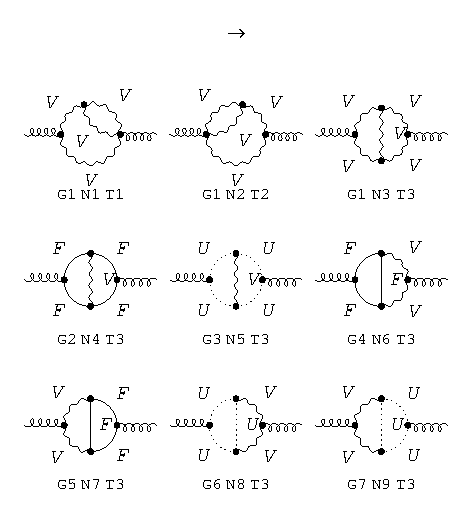
\includegraphics{qcd2loopgluon-tex_gr1}}
\scalebox{1.0}{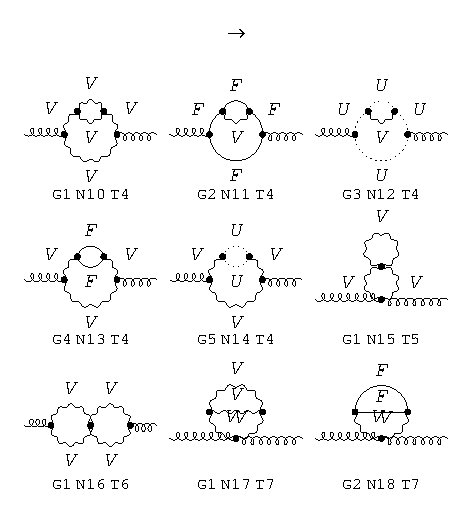
\includegraphics{qcd2loopgluon-tex_gr2}}
\scalebox{1.0}{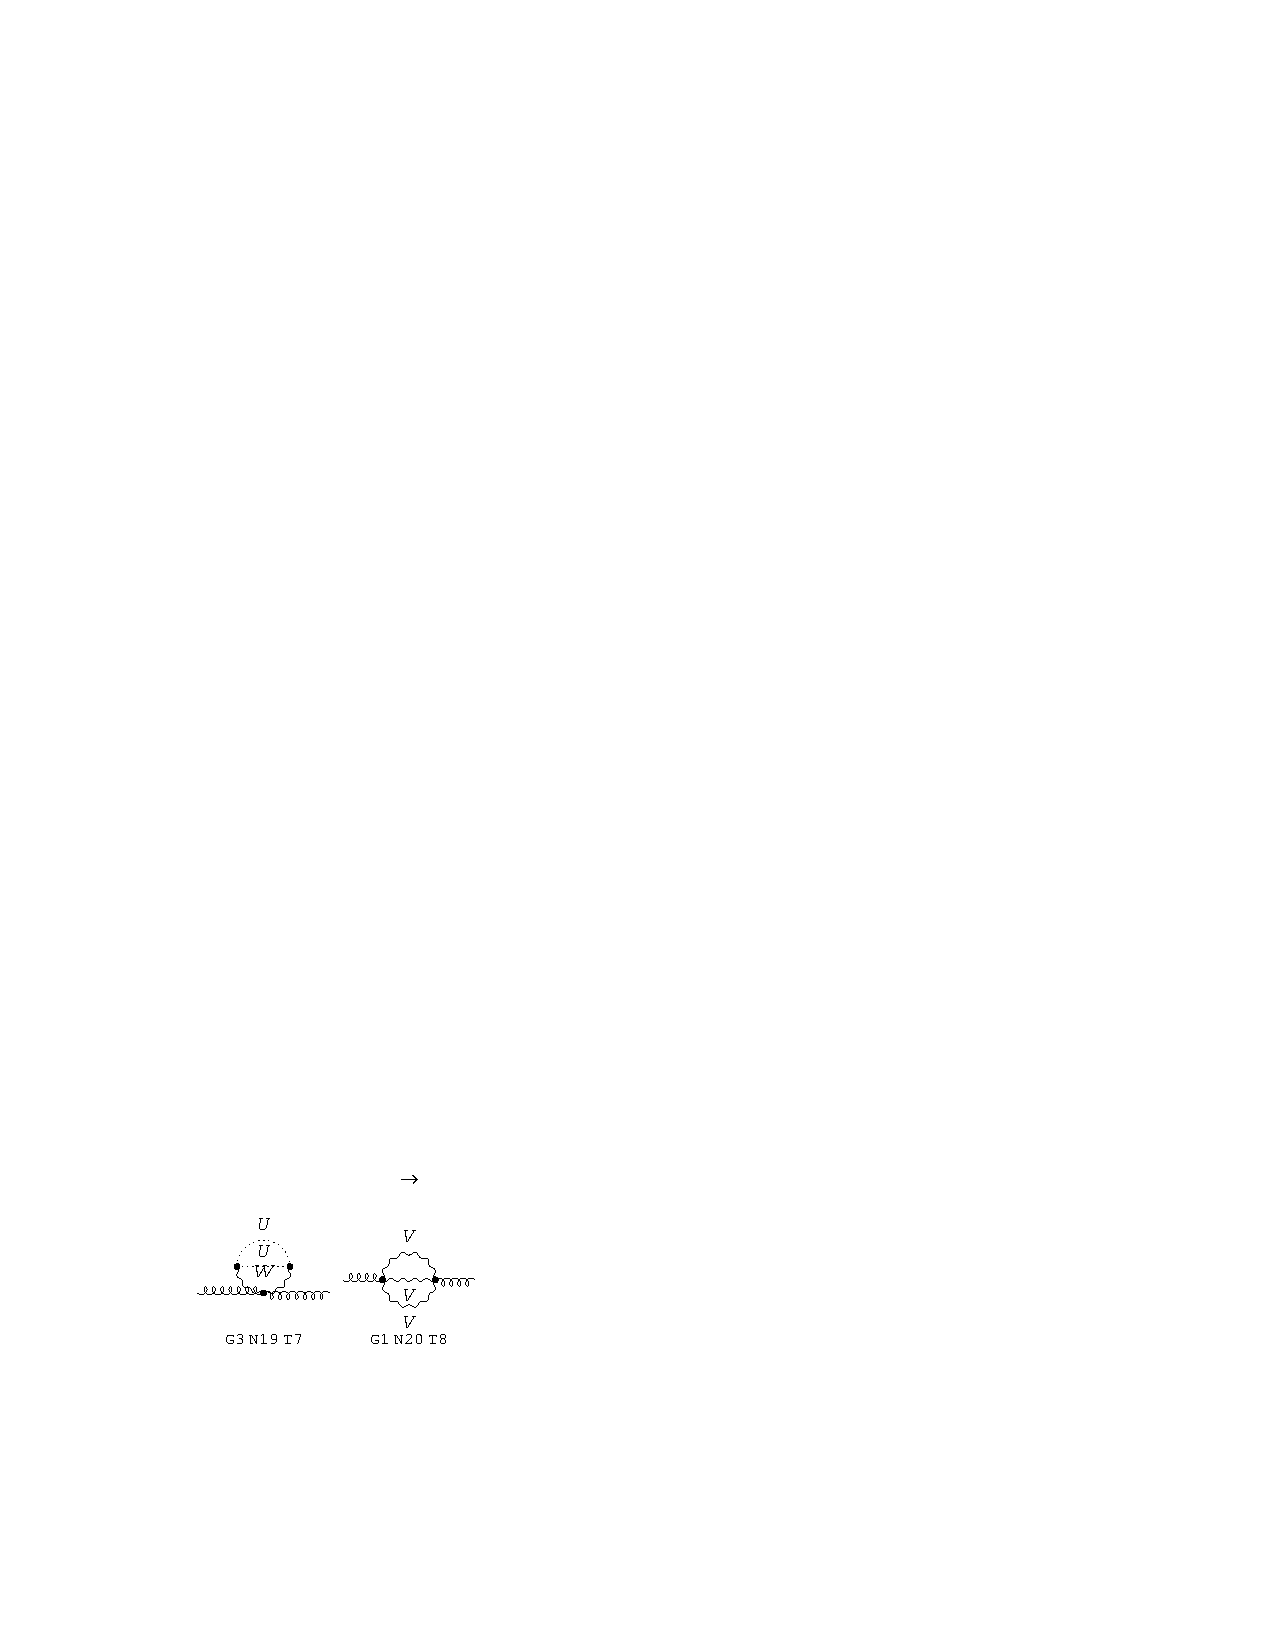
\includegraphics{qcd2loopgluon-tex_gr3}}
\caption{2-loop gluon self-energy diagrams.}
\end{center}
\end{figure}

\Subsubsection*{Calculating the bare 2-loop on-shell gluon self energy diagrams}

In the Model file incoming momenta are specified by \mb{p1}, \mb{p2}, ... and all outgoing
by \mb{k1}, \mb{k2}, .. .\\
We substitute p1 to p and k1 to -p and do some further substitutions.

\begin{CellGroup}

\dispSFinmath{
\MathBegin{MathArray}{l}
\Mvariable{amps}=\Muserfunction{CreateFeynAmp}[
       \Mvariable{inserts},\Mvariable{Truncated}\rightarrow \Mvariable{True},\Mvariable{PreFactor}\rightarrow 1]/.
      \Mvariable{k1}\rightarrow -\Mvariable{p1}/.\Mvariable{p1}\rightarrow p/.  \\
\noalign{\vspace{0.555556ex}}
\hspace{3.em} 
          \Muserfunction{FeynAmpList}[\_\_]\RuleDelayed \Mvariable{List}\multsp /.\multsp 
      \Muserfunction{FeynAmp}[\_,\_,\Mvariable{x\_}]\RuleDelayed x;\\
\MathEnd{MathArray}
}

\dispSFinmath{
\Muserfunction{amps}[[3]]
}

\dispTFoutmath{
\MathBegin{MathArray}{l}
\frac{1}{2}\multsp \Pi _{g}^{\Mvariable{li9}\Mvariable{li10}}(p-{q_1})\multsp 
   \Pi _{g}^{\Mvariable{li3}\Mvariable{li4}}({q_1})\multsp \Pi _{g}^{\Mvariable{li11}\Mvariable{li12}}(-p-{q_2})\multsp 
   \Pi _{g}^{\Mvariable{li5}\Mvariable{li6}}({q_2})\multsp \Pi _{g}^{\Mvariable{li7}\Mvariable{li8}}({q_1}+{q_2})\multsp \\
   {V^{\Mvariable{li1}\Mvariable{li4}\Mvariable{li10}}}(p,\multsp {q_1},\multsp p-{q_1})\multsp
   {V^{\Mvariable{li2}\Mvariable{li6}\Mvariable{li12}}}(p,\multsp {q_2},\multsp -p-{q_2})\multsp   \\
\noalign{\vspace{0.840278ex}}
   \hspace{1.em}
   {V^{\Mvariable{li3}\Mvariable{li5}\Mvariable{li8}}}(-{q_1},\multsp -{q_2},\multsp {q_1}+{q_2})\multsp 
   {V^{\Mvariable{li7}\Mvariable{li9}\Mvariable{li11}}}(-{q_1}-{q_2},\multsp {q_1}-p,\multsp p+{q_2})\multsp  \\
   {f_{\Mvariable{ci1}\Mvariable{ci4}\Mvariable{ci10}}}\multsp {f_{\Mvariable{ci2}\Mvariable{ci5}\Mvariable{ci11}}}\multsp 
   {f_{\Mvariable{ci4}\Mvariable{ci5}\Mvariable{ci8}}}\multsp {f_{\Mvariable{ci8}\Mvariable{ci10}\Mvariable{ci11}}}
\MathEnd{MathArray}
}

\dispSFinmath{
\Mvariable{amp31}=\Muserfunction{amps}[[3]]/.\Mvariable{q2}\rightarrow -\Mvariable{q2}
}

\dispTFoutmath{
\MathBegin{MathArray}{l}
\frac{1}{2}\multsp \Pi _{g}^{\Mvariable{li9}\Mvariable{li10}}(p-{q_1})\multsp 
   \Pi _{g}^{\Mvariable{li3}\Mvariable{li4}}({q_1})\multsp \Pi _{g}^{\Mvariable{li7}\Mvariable{li8}}({q_1}-{q_2})\multsp 
   \Pi _{g}^{\Mvariable{li5}\Mvariable{li6}}({q_2})\multsp \Pi _{g}^{\Mvariable{li11}\Mvariable{li12}}({q_2}-p)\multsp \\
   {V^{\Mvariable{li1}\Mvariable{li4}\Mvariable{li10}}}(p,\multsp {q_1},\multsp p-{q_1})\multsp 
   {V^{\Mvariable{li2}\Mvariable{li6}\Mvariable{li12}}}(p,\multsp -{q_2},\multsp {q_2}-p)\multsp   \\
\noalign{\vspace{0.840278ex}}
   \hspace{1.em} {V^{\Mvariable{li3}\Mvariable{li5}\Mvariable{li8}}}(-{q_1},\multsp {q_2},\multsp {q_1}-{q_2})\multsp 
   {V^{\Mvariable{li7}\Mvariable{li9}\Mvariable{li11}}}({q_2}-{q_1},\multsp {q_1}-p,\multsp p-{q_2})\multsp \\
   {f_{\Mvariable{ci1}\Mvariable{ci4}\Mvariable{ci10}}}\multsp {f_{\Mvariable{ci2}\Mvariable{ci5}\Mvariable{ci11}}}\multsp 
   {f_{\Mvariable{ci4}\Mvariable{ci5}\Mvariable{ci8}}}\multsp {f_{\Mvariable{ci8}\Mvariable{ci10}\Mvariable{ci11}}}\\
\MathEnd{MathArray}
}

\dispSFinmath{
\Muserfunction{amp31}//\Mfunction{InputForm}
}

\dispTFoutmath{
\MathBegin{MathArray}{l}
(\Muserfunction{GluonPropagator}[
     p\multsp -\multsp \Mvariable{q1},\multsp \{\Mvariable{li9}\},\multsp \{\Mvariable{li10}\}]*  \\
\noalign{\vspace{0.625ex}}\multsp
    \multsp \Muserfunction{GluonPropagator}[\Mvariable{q1},\multsp \{\Mvariable{li3}\},\multsp \{\Mvariable{li4}\}]*  \\
   \noalign{\vspace{0.625ex}}\multsp \multsp \Muserfunction{GluonPropagator}[
    \Mvariable{q1}\multsp -\multsp \Mvariable{q2},\multsp \{\Mvariable{li7}\},\multsp \{\Mvariable{li8}\}]*  \\
   \noalign{\vspace{0.625ex}}\multsp \multsp \Muserfunction{GluonPropagator}[
    \Mvariable{q2},\multsp \{\Mvariable{li5}\},\multsp \{\Mvariable{li6}\}]*  \\
\noalign{\vspace{0.625ex}}\multsp \multsp 
   \Muserfunction{GluonPropagator}[-p\multsp +\multsp \Mvariable{q2},\multsp \{\Mvariable{li11}\},\multsp \{\Mvariable{li12}\}]*  \\
   \noalign{\vspace{0.625ex}}\multsp \multsp \Muserfunction{GluonVertex}[
    \{p,\multsp \Mvariable{li1}\},\multsp \{\Mvariable{q1},\multsp \Mvariable{li4}\},\multsp 
     \{p\multsp -\multsp \Mvariable{q1},\multsp \Mvariable{li10}\}]*  \\
\noalign{\vspace{0.625ex}}\multsp \multsp 
   \Muserfunction{GluonVertex}[\{p,\multsp \Mvariable{li2}\},\multsp \{-\Mvariable{q2},\multsp \Mvariable{li6}\},\multsp 
     \{-p\multsp +\multsp \Mvariable{q2},\multsp \Mvariable{li12}\}]*  \\
\noalign{\vspace{0.625ex}}\multsp \multsp 
   \Muserfunction{GluonVertex}[\{-\Mvariable{q1},\multsp \Mvariable{li3}\},\multsp \{\Mvariable{q2},\multsp \Mvariable{li5}\},\multsp 
     \{\Mvariable{q1}\multsp -\multsp \Mvariable{q2},\multsp \Mvariable{li8}\}]*  \\
\noalign{\vspace{0.625ex}}\multsp \multsp 
   \Muserfunction{GluonVertex}[\{-\Mvariable{q1}\multsp +\multsp \Mvariable{q2},\multsp \Mvariable{li7}\},\multsp 
     \{-p\multsp +\multsp \Mvariable{q1},\multsp \Mvariable{li9}\},\multsp   \\
\noalign{\vspace{0.625ex}}\multsp \multsp \multsp 
     \{p\multsp -\multsp \Mvariable{q2},\multsp \Mvariable{li11}\}]*
   \Muserfunction{SUNF}[\Mvariable{ci1},\multsp \Mvariable{ci4},\multsp \Mvariable{ci10}]*  \\
\noalign{\vspace{0.625ex}}\multsp \multsp 
   \Muserfunction{SUNF}[\Mvariable{ci2},\multsp \Mvariable{ci5},\multsp \Mvariable{ci11}]*
   \Muserfunction{SUNF}[\Mvariable{ci4},\multsp \Mvariable{ci5},\multsp \Mvariable{ci8}]*  \\
\noalign{\vspace{0.625ex}}\multsp \multsp 
     \Muserfunction{SUNF}[\Mvariable{ci8},\multsp \Mvariable{ci10},\multsp \Mvariable{ci11}])/2\\
\MathEnd{MathArray}
}

\dispSFinmath{
\Mvariable{amp32}=\Muserfunction{SUNSimplify}[\Mvariable{Explicit}@\multsp \Mvariable{amp31}]
}

\dispTFoutmath{
\MathBegin{MathArray}{l}
-\big(\ImaginaryI \multsp C_{A}^{2}\multsp \\ {g^{\Mvariable{li10}\Mvariable{li9}}}\multsp 
     {g^{\Mvariable{li11}\Mvariable{li12}}}\multsp {g^{\Mvariable{li3}\Mvariable{li4}}}\multsp 
     \big(-{p^{\Mvariable{li1}}}\multsp {g^{\Mvariable{li10}\Mvariable{li4}}}+
       2\multsp q_{1}^{\Mvariable{li1}}\multsp {g^{\Mvariable{li10}\Mvariable{li4}}}+
       {g^{\Mvariable{li1}\Mvariable{li4}}}\multsp {p^{\Mvariable{li10}}}-
       {g^{\Mvariable{li1}\Mvariable{li4}}}\multsp q_{1}^{\Mvariable{li10}}-
       {g^{\Mvariable{li1}\Mvariable{li10}}}\multsp q_{1}^{\Mvariable{li4}}\big)\multsp   \\
\noalign{\vspace{0.659722ex}}
   {g^{\Mvariable{li5}\Mvariable{li6}}}\multsp 
   \big({p^{\Mvariable{li12}}}\multsp {g^{\Mvariable{li2}\Mvariable{li6}}}+
     q_{2}^{\Mvariable{li12}}\multsp {g^{\Mvariable{li2}\Mvariable{li6}}}+
     {g^{\Mvariable{li12}\Mvariable{li6}}}\multsp {p^{\Mvariable{li2}}}-
     2\multsp {g^{\Mvariable{li12}\Mvariable{li6}}}\multsp q_{2}^{\Mvariable{li2}}-
     2\multsp {g^{\Mvariable{li12}\Mvariable{li2}}}\multsp {p^{\Mvariable{li6}}}+
     {g^{\Mvariable{li12}\Mvariable{li2}}}\multsp q_{2}^{\Mvariable{li6}}\big)\multsp   \\
\noalign{\vspace{0.659722ex}}
    {g^{\Mvariable{li7}\Mvariable{li8}}}\multsp 
   \big(-q_{1}^{\Mvariable{li3}}\multsp {g^{\Mvariable{li5}\Mvariable{li8}}}+
     2\multsp q_{2}^{\Mvariable{li3}}\multsp {g^{\Mvariable{li5}\Mvariable{li8}}}+
     2\multsp {g^{\Mvariable{li3}\Mvariable{li8}}}\multsp q_{1}^{\Mvariable{li5}}-
     {g^{\Mvariable{li3}\Mvariable{li8}}}\multsp q_{2}^{\Mvariable{li5}}-
     {g^{\Mvariable{li3}\Mvariable{li5}}}\multsp q_{1}^{\Mvariable{li8}}-
     {g^{\Mvariable{li3}\Mvariable{li5}}}\multsp q_{2}^{\Mvariable{li8}}\big)\multsp   \\
\noalign{\vspace{0.659722ex}}
    \big({p^{\Mvariable{li11}}}\multsp {g^{\Mvariable{li7}\Mvariable{li9}}}-
     2\multsp q_{1}^{\Mvariable{li11}}\multsp {g^{\Mvariable{li7}\Mvariable{li9}}}+
     q_{2}^{\Mvariable{li11}}\multsp {g^{\Mvariable{li7}\Mvariable{li9}}}-
     2\multsp {g^{\Mvariable{li11}\Mvariable{li9}}}\multsp {p^{\Mvariable{li7}}}+
     {g^{\Mvariable{li11}\Mvariable{li9}}}\multsp q_{1}^{\Mvariable{li7}}+
     {g^{\Mvariable{li11}\Mvariable{li9}}}\multsp q_{2}^{\Mvariable{li7}}+\\
     {g^{\Mvariable{li11}\Mvariable{li7}}}\multsp {p^{\Mvariable{li9}}}+
     {g^{\Mvariable{li11}\Mvariable{li7}}}\multsp q_{1}^{\Mvariable{li9}}-
     2\multsp {g^{\Mvariable{li11}\Mvariable{li7}}}\multsp q_{2}^{\Mvariable{li9}}\big)\multsp
     {{\delta }_{\Mvariable{ci1}\Mvariable{ci2}}}\big)\big/\\
\noalign{\vspace{0.659722ex}}
   \hspace{4.em}
   \big(4\multsp {{(p-{q_1})}^2}\multsp q_{1}^{2}\multsp {{({q_1}-{q_2})}^2}\multsp q_{2}^{2}\multsp {{({q_2}-p)}^2}\big)\\
   \MathEnd{MathArray}
}

\dispSFinmath{
\MathBegin{MathArray}{l}
\Mvariable{Timing}[  \\
\noalign{\vspace{0.555556ex}}
\hspace{1.em} \Mvariable{amp33}=  \\
   \noalign{\vspace{0.555556ex}}
\hspace{2.em} \Muserfunction{Collect2}[\Mvariable{FeynAmpDenominatorCombine}@  \\
\noalign{\vspace{
   0.555556ex}}
\hspace{4.em} \Muserfunction{Contract3}[
         \Muserfunction{Explicit}[\Mvariable{amp32}]/.\Mvariable{li1}\rightarrow \Mvariable{li2}/.
          \Muserfunction{SUNDelta}[\_\_]\RuleDelayed 1],\Mvariable{q1},\Mvariable{q2}];]\\
\MathEnd{MathArray}
}

\dispTFoutmath{
\{0.71\multsp \Mvariable{Second},\Mvariable{Null}\}
}

\dispSFinmath{
\Mvariable{amp33}
}

\dispTFoutmath{
\MathBegin{MathArray}{l}
-\frac{\ImaginaryI \multsp C_{A}^{2}\multsp (11-5\multsp D)\multsp {{p\cdot {q_1}}^2}}
     {2\multsp q_{1}^{2}.q_{2}^{2}.{{(p-{q_1})}^2}.{{({q_2}-p)}^2}.{{({q_1}-{q_2})}^2}}-
   \frac{\ImaginaryI \multsp C_{A}^{2}\multsp (5-2\multsp D)\multsp {{{q_1}\cdot {q_2}}^2}}
    {2\multsp q_{1}^{2}.q_{2}^{2}.{{(p-{q_1})}^2}.{{({q_2}-p)}^2}.{{({q_1}-{q_2})}^2}}-  \\
\noalign{\vspace{1.47917ex}}
   \frac{3\multsp \ImaginaryI \multsp C_{A}^{2}\multsp (1-D)\multsp {p^2}\multsp p\cdot {q_1}}
    {2\multsp q_{1}^{2}.q_{2}^{2}.{{(p-{q_1})}^2}.{{({q_2}-p)}^2}.{{({q_1}-{q_2})}^2}}+
   \frac{\ImaginaryI \multsp C_{A}^{2}\multsp (34-19\multsp D)\multsp p\cdot {q_1}\multsp p\cdot {q_2}}
    {2\multsp q_{1}^{2}.q_{2}^{2}.{{(p-{q_1})}^2}.{{({q_2}-p)}^2}.{{({q_1}-{q_2})}^2}}+\\
\noalign{\vspace{1.47917ex}}
   \frac{\ImaginaryI \multsp C_{A}^{2}\multsp (7-4\multsp D)\multsp {p^2}\multsp q_{1}^{2}}
    {q_{1}^{2}.q_{2}^{2}.{{(p-{q_1})}^2}.{{({q_2}-p)}^2}.{{({q_1}-{q_2})}^2}}-
    \frac{
       \ImaginaryI \multsp C_{A}^{2}\multsp (14-11\multsp D)\multsp p\cdot {q_2}\multsp q_{1}^{2}}{2\multsp 
      q_{1}^{2}.q_{2}^{2}.{{(p-{q_1})}^2}.{{({q_2}-p)}^2}.{{({q_1}-{q_2})}^2}}-\\
\noalign{\vspace{1.47917ex}}
   \frac{5\multsp \ImaginaryI \multsp C_{A}^{2}\multsp (5-2\multsp D)\multsp {p^2}\multsp {q_1}\cdot {q_2}}
    {2\multsp q_{1}^{2}.q_{2}^{2}.{{(p-{q_1})}^2}.{{({q_2}-p)}^2}.{{({q_1}-{q_2})}^2}}+
   \frac{\ImaginaryI \multsp C_{A}^{2}\multsp (5-2\multsp D)\multsp p\cdot {q_1}\multsp {q_1}\cdot {q_2}}
    {2\multsp q_{1}^{2}.q_{2}^{2}.{{(p-{q_1})}^2}.{{({q_2}-p)}^2}.{{({q_1}-{q_2})}^2}}+  \\
\noalign{\vspace{1.47917ex}}
   \frac{\ImaginaryI \multsp C_{A}^{2}\multsp (5-2\multsp D)\multsp p\cdot {q_2}\multsp {q_1}\cdot {q_2}}
    {2\multsp q_{1}^{2}.q_{2}^{2}.{{(p-{q_1})}^2}.{{({q_2}-p)}^2}.{{({q_1}-{q_2})}^2}}-
   \frac{\ImaginaryI \multsp C_{A}^{2}\multsp (14-11\multsp D)\multsp p\cdot {q_1}\multsp q_{2}^{2}}
    {2\multsp q_{1}^{2}.q_{2}^{2}.{{(p-{q_1})}^2}.{{({q_2}-p)}^2}.{{({q_1}-{q_2})}^2}}+\\
\noalign{\vspace{1.47917ex}}
   \frac{\ImaginaryI \multsp C_{A}^{2}\multsp (14-11\multsp D)\multsp q_{1}^{2}\multsp q_{2}^{2}}
    {2\multsp q_{1}^{2}.q_{2}^{2}.{{(p-{q_1})}^2}.{{({q_2}-p)}^2}.{{({q_1}-{q_2})}^2}}\\
\MathEnd{MathArray}
}

\dispSFinmath{
\Mvariable{amp34}=\Muserfunction{ToTFi}[\Mvariable{amp33},\Mvariable{q1},\Mvariable{q2},p]//\Muserfunction{FCE}
}

\dispTFoutmath{
\MathBegin{MathArray}{l}
-\frac{5}{2}\multsp \ImaginaryI \multsp (5-2\multsp D)\multsp {p^2}\multsp 
    F_{\{1,0\}\{1,0\}\{1,0\}\{1,0\}\{1,0\}}^{(D)\multsp 00001}\multsp C_{A}^{2}-
   \frac{1}{2}\multsp \ImaginaryI \multsp (5-2\multsp D)\multsp F_{\{1,0\}\{1,0\}\{1,0\}\{1,0\}\{1,0\}}^{(D)\multsp 00002}\multsp 
    C_{A}^{2}+  \\
\noalign{\vspace{1.10417ex}}
\frac{1}{2}\multsp \ImaginaryI \multsp (5-2\multsp D)\multsp 
    F_{\{1,0\}\{1,0\}\{1,0\}\{1,0\}\{1,0\}}^{(D)\multsp 00011}\multsp C_{A}^{2}-
   \frac{3}{2}\multsp \ImaginaryI \multsp (1-D)\multsp {p^2}\multsp F_{\{1,0\}\{1,0\}\{1,0\}\{1,0\}\{1,0\}}^{(D)\multsp 00100}\multsp 
    C_{A}^{2}+\\
\noalign{\vspace{1.10417ex}}\frac{1}{2}\multsp \ImaginaryI \multsp (5-2\multsp D)\multsp F_{\{1,0\}\{1,0\}\{1,0\}\{1,0\}\{1,0\}}^{(D)\multsp 00101}
    \multsp C_{A}^{2}+
\frac{1}{2}\multsp \ImaginaryI \multsp (34-19\multsp D)\multsp 
    F_{\{1,0\}\{1,0\}\{1,0\}\{1,0\}\{1,0\}}^{(D)\multsp 00110}\multsp C_{A}^{2}-\\
\noalign{\vspace{1.10417ex}}
   \frac{1}{2}\multsp \ImaginaryI \multsp (11-5\multsp D)\multsp F_{\{1,0\}\{1,0\}\{1,0\}\{1,0\}\{1,0\}}^{(D)\multsp 00200}\multsp 
    C_{A}^{2}-
\frac{1}{2}\multsp \ImaginaryI \multsp (14-11\multsp D)\multsp F_{\{1,0\}\{1,0\}\{1,0\}\{1,0\}\{1,0\}}^{(D)\multsp 01100}
    \multsp C_{A}^{2}+  \\
\noalign{\vspace{1.10417ex}}
\ImaginaryI \multsp (7-4\multsp D)\multsp {p^2}\multsp 
    F_{\{1,0\}\{1,0\}\{1,0\}\{1,0\}\{1,0\}}^{(D)\multsp 10000}\multsp C_{A}^{2}-
   \frac{1}{2}\multsp \ImaginaryI \multsp (14-11\multsp D)\multsp F_{\{1,0\}\{1,0\}\{1,0\}\{1,0\}\{1,0\}}^{(D)\multsp 10010}\multsp 
    C_{A}^{2}+\\
\noalign{\vspace{1.10417ex}}
\frac{1}{2}\multsp \ImaginaryI \multsp (14-11\multsp D)\multsp F_{\{1,0\}\{1,0\}\{1,0\}\{1,0\}\{1,0\}}^{(D)\multsp 11000}
    \multsp C_{A}^{2}\\
\MathEnd{MathArray}
}

\dispSFinmath{
\Mvariable{amp35}=\Muserfunction{TarcerRecurse}[\Mvariable{amp34}]
}

\dispTFoutmath{
-\frac{\ImaginaryI \multsp (2\multsp {D^2}-57\multsp D+136)\multsp {p^2}\multsp {{B_{\{1,0\}\{1,0\}}^{(D)}}^2}\multsp C_{A}^{2}}
     {16\multsp (D-4)}-\frac{\ImaginaryI \multsp (2\multsp {D^3}+19\multsp {D^2}-124\multsp D+184)\multsp J_{\{1,0\}\{1,0\}\{1,0\}}^{(D)}
      \multsp C_{A}^{2}}{4\multsp {{(D-4)}^2}}
}

\end{CellGroup}

\section{Applications in Chiral Perturbation Theory}

\subsection{Introduction}

The subpackage \fphi provides utilities for computations in the Chiral Perturbation Theory (ChPT). The general idea is to allow writing up a calculation starting with a lagrangian and ending up with an amplitude, all within the framework of \fc. For this to be possible, many functions on a rather general level were implemented, as was a method of interacting seamlessly with \fa. The following sections cover the more important features of the package. A fuller description can be found in \cite{PHI}.

The motivation for writing \fphi was a lack of software for implementing an effective model like one of the various ChPT models, which have a more complicated power counting than models which simply expand Green's functions perturbatively in a coupling constant. However, the package is general enough that other models can be defined, as has been demonstrated with the simple example of QED. Given the many effective models that already exist and the many new ones that keep coming, it is the hope of the author that this software might be of use also outside the realm of ChPT.

The main features of \fphi are:
\begin{itemize}
\item A set of basic objects are provided that can be composed and manipulated to form ChPT lagrangians.
\item The most common ChPT lagrangians are included and new ones can easily be defined.
\item The lagrangians can be expanded in terms of pion (meson) fields, with SU(2) (SU(3)) flavour traces being done automatically.
\item External sources can be switched off and on.
\item \fa is used for generating Feynman diagrams and amplitudes, including counter-terms. Power counting and storing of Feynman rules is systematized.
\end{itemize}

\subsection{Chiral quantum fields and lagrangians}

\fphi comes with a number of predefined chiral models (or configurations). These define lagrangians etc. in terms of quantum fields. Which configuration and lagrangians are loaded should be defined before startup of \fc. The list of available configurations and lagrangians can be found by browsing the directory "HighEnergyPhysics/Phi/Configurations" and "HighEnergyPhysics/Phi/Lagrangians".
\beom
\dtog{
Quit[];\\\\
\$LoadPhi = True;\\
\$LoadFeynArts = True;\\
\$Configuration = "ChPTVirtualPhotons2";\\
\$Lagrangians = {"ChPTVirtualPhotons2"[2], \\
\mindent "ChPTVirtualPhotons2"[4]};\\\\
Get["HighEnergyPhysics`FeynCalc`"];\\}{}{Quit the kernel and reload \fc with the packages \fphi and \fa enabled. We may specify to load the some \fphi model and lagrangians, in this case we choose "ChPTVirtualPhotons2" and its two lagrangians.}
\domtog{}{}{The database of lagrangians has been enlarged with lagrangians specified. We may inspect one of them. In section \ref{chptLags} we shall discuss how to construct such lagrangians.}
\enom
\otabtwo{
\mbs{\$Configuration} & string variable determining which configuration is loaded at startup\cr
\mbs{\$Lagrangians} & string variable determining which lagrangians are loaded at startup\cr
}{\fphi startup settings.}
The field argument of \mb{QuantumField} can be any symbol. Notice however, that the various configurations files for \fphi each use some conventions; e.g. for a pion the symbol \mb{Particle[Pion]} is used. The Dirac bar can be applied to fermionic \mb{QuantumField}s with the function \mb{DiracBar}. Since partial derivatives and covariant derivatives may be performed on \mb{QuantumField}s as well as on polynomials of \mb{QuantumField}s, the \mb{QuantumField}s usually carry a space-time argument, e.g. $x$. \mb{QuantumField}s may be grouped in SU($N$) matrices or vectors\footnote{in the rest of this section, with  SU($N$) we shall understand  SU($N$), where $N=2 or 3$.} with the functions \mb{IsoVector}, \mb{UMatrix} and \mb{UVector} as heads\footnote{When this is done, these functions take over the space-time argument.}. These things are illustrated through the following initial simple examples.
\beom
\domtog{
\mb{CovariantFieldDerivative[QuantumField[Particle[\\
\mindent Pion]][x]\phat 2, x, LorentzIndex[$\bm{\mu}$]]//\\
CommutatorReduce}
}{
$\ComplexI \pi^2\, \left( \overrightarrow{V_\mu} \cdot
               \overrightarrow{\bm{\sigma}}\, -\,
                     \overrightarrow{A_\mu} \cdot \overrightarrow{\bm{\sigma}}
                     \right)\, -\, 
\ComplexI \left( \overrightarrow{A_\mu} \cdot \overrightarrow{\bm{\sigma}}\, +\,
                \overrightarrow{V_\mu} \cdot \overrightarrow{\bm{\sigma}}\right)
                     \pi^2 \, +\,\\
\ComplexI \gamma_\mu Q_{\rm\bf L}\, \pi^2\, -\, \ComplexI \gamma_\mu Q_{\rm\bf R}\, \pi^2\, +
2\pi\, \partial_\mu\pi$
}{Here is how to enter a covariant derivative $D_\mu(\phi_\pi(x)^2$).\\
Notice that this model defines the covariant derivative and assigns the symbol $\pi$ to the field $\phi_\pi$.}
\domtog{
\mb{CovariantFieldDerivative[IsoDot[\\
    IsoVector[QuantumField[Particle[Pion]]][x],\\
      IsoVector[UMatrix[UGenerator[]]]], x,\\
    LorentzIndex[$\bm{\mu}$]] // CommutatorReduce}
}{
$\partial_\mu\left(\overrightarrow{\pi}\right) \cdot \overrightarrow{\bm{\sigma}}\, +\\
 \ComplexI \left( \overrightarrow{\pi} \cdot
 \overrightarrow{\bm{\sigma}}\, \SixPointedStar\, \left( \overrightarrow{V_\mu} \cdot
               \overrightarrow{\bm{\sigma}} -
                     \overrightarrow{A_\mu} \cdot \overrightarrow{\bm{\sigma}}
                     \right)\right) -
\ComplexI \left( \left( \overrightarrow{V_\mu} \cdot
               \overrightarrow{\bm{\sigma}} +
                     \overrightarrow{A_\mu} \cdot \overrightarrow{\bm{\sigma}}
                     \right)\, \SixPointedStar\,  \overrightarrow{\pi} \cdot
\overrightarrow{\bm{\sigma}} \right) \, +\\
\ComplexI \left( \overrightarrow{\pi} \cdot
 \overrightarrow{\bm{\sigma}}\, \SixPointedStar\, Q_{\rm\bf L}\right)\, \gamma_\mu\, -\,
\ComplexI \left( Q_{\rm\bf R}\, \SixPointedStar\,  \overrightarrow{\pi} \cdot
 \overrightarrow{\bm{\sigma}} \right)\, \gamma_\mu$
}{
Here is a more complex example, involving also \mb{IsoVector}, \mb{UMatrix}. Notice that
\mb{IsoVector} takes over the $x$-dependence.
}
\domtog{
\mb{UVector[DiracBar[QuantumField[Particle[\\
   \mindent Nucleon]]]][x].\\
    DiracGamma[LorentzIndex[$\bm{\mu}$]].\\
    NM[UMatrix[SMM][x], \\
      \mindent FieldDerivative[Adjoint[UMatrix[SMM][x]], \\
      \mindent \mindent x, LorentzIndex[$\bm{\mu}$]]].\\
    UVector[QuantumField[Particle[Nucleon]]][x]}
}{$\vec{\overline{\rm N}}\, .\, \gamma^\mu\, .\, u\, \SixPointedStar\, \partial_\mu(u^\dagger)\, .\, \vec{{\rm N}}$}{Although the model "ChPTVirtualPhotons2" does not use nucleons, we may still use e.g. the SU($N$) construction $\overrightarrow{\bar{\psi}_{\rm N}}\, \gamma^\mu\, u \partial_\mu\, u^\dag\, \overrightarrow{\psi_{\rm N}}$, where $u$ is a $N \times N$ field matrix containing the meson fields (see e.g. \cite{Ecker:1992jh}).}
\enom
\mb{FieldDerivative} and \mb{CovariantFieldDerivative} are derivatives acting on the \mb{QuantumField}s\footnote{A different but equivalent way of calculating derivatives
is using ``\mb{$.$}'' and the operators of page \pageref{partialDs}. The ``\mb{$.$}'' operator is, however, also used for multiplying Dirac matrices, so to avoid confusion \mb{FieldDerivative} may be used.}.
The \mma \mb{Dot} is used for multiplication of Dirac matrices and the multiplication of SU($N$) matrices with SU($N$) vectors, \mb{NM} (``\mb{$\SixPointedStar$}'' in \mb{OutputForm}) is used for multiplication of SU($N$) matrices, \mb{IsoDot} (``\mb{$\cdot$}'' in \mb{OutputForm}) is used for multiplication of SU($N$) iso-vectors, \mb{UGenerator} denotes generators of SU($N$), \mb{CommutatorReduce} pulls out abelian quantities of non-abelian products. These functions are introduced more systematically in the following section.

\otabtwo{
\mbs{\mb{FieldDerivative[g[x], x, \{l1, l2, ...\}]}} & calculates
$\frac{\partial}{\partial x_{l1}}\frac{\partial}{\partial x_{l2}}\ldots$ on the
expression \mb{g[x]}\cr
\mbs{\mb{CovariantFieldField Derivative[g[x], x, \{l1, l2, ...\}]}} &
as above but with the vector and axial-vector source field  terms included. This is
defined in the chosen configuration file\cr
}{Derivatives acting on \mb{QuantumField}s.}

Many operations can be performed on expressions like the ones above. We shall see some in the ChPT examples to come. But first we turn to some of the objects that \fphi adds to the basic framework of \fc. Of the many utilities, we shall focus on SU($N$) functions and the interaction with \fa. Notice that in ChPT, a condensed notation is used and objects like \mb{MM[x]} and \mb{SMM[x]} actually contain \mb{QuantumField}s. Remember that an explanation of the various symbols can be obtained by using the \mb{?} operator.

\subsection{Chiral vectors, matrices and structure constants in SU(2) and SU(3)}

\otabtwo{
\mbs{IsoVector[{\sl v}]} & represents an SU(2) or SU(3) multiplet with number of
entries corresponding to the number of generators (3 or 8)\cr
\mbs{UVector[{\sl v}]} & represents an SU(2) or SU(3) vector with number of entries
corresponding to the dimension of the representation (2 or 3)\cr
\mbs{UMatrix[{\sl m}]} & is recognized as a square matrix of dimension 2 or 3\cr
}{SU($N$) vectors and matrices.}

\otabthree{
{\sl option name} & {\sl default value} &\cr
\hhline
\mbs{SUNN[{\sl v}]} & number of quark flavours. Either 2 or 3 & \mb{2} \cr
\mbs{UDimension[{\sl v}]} & dimension of the representation & \mb{Automatic}\cr
}{Options determining the dimension of SU($N$) vectors and matrices.}

Several way are provided to work with SU($N$) vectors and matrices. One can work directly with the vectors and matrices using the multiplications listed below.

\otabtwo{
\mbs{NM[{\sl a}, {\sl b}, \ldots]} & non-commutative multiplication for matrices and/or fields {\sl a}, {\sl b}, \ldots \cr
\mbs{IsoDot[{\sl a}, {\sl b}]} & dot product for iso-vectors {\sl a}, {\sl b}\cr
\mbs{IsoCross[{\sl a}, {\sl b}]} & anti-symmetric cross product for isospin vectors {\sl a}, {\sl b}\cr
\mbs{IsoSymmetricCross} & symmetric cross product for isospin vectors {\sl a}, {\sl b}\cr
}{Multiplication operators for SU($N$) vectors and matrices.}

Another possibility  is to write out the components explicitly, using the functions listed below.

\otabtwo{
\mbs{WriteOutUMatrices[{\sl exp}]} & write out SU($N$) vectors in {\sl exp}\cr
\mbs{WriteOutIsoVectors[{\sl exp}]} & write out SU($N$) matrices in {\sl exp}\cr
}{Writing out explicit components of SU($N$) vectors and matrices.}

A third possibility is to work with the components using symbolic indices.

\otabtwo{
\mbs{IsoIndicesSupply[{\sl exp}]} & replaces dot and cross products of SU($N$) vectors with
contracted indices\cr
\mbs{IndicesCleanup[{\sl exp}]} & renames Lorentz and SU($N$) indices in a systematic way\cr
\mbs{SUNReduce[{\sl exp}]} & does some reduction on expressions involving SU($N$) indices\cr
}{Writing out components of SU($N$) vectors and matrices using symbolic indices and cleaning up afterwards.}

\otabtwo{
\mbs{CommutatorReduce[{\sl exp}]} & does some reduction on expressions containing non-abelian  SU($N$) products in {\sl exp}\cr
}{Reducing non-abelian  SU($N$) products.}

UGenerator, SU2Delta, SU2F, ...

\subsection{Chiral lagrangians}
\label{chptLags}

\subsection{Chiral divergent one-loop generating functionals}

\subsection{Chiral power counting with \fa}

The database of amplitudes has been enlarged with all amplitudes calculated and stored using \mb{CheckF}

\subsection{Example:\; $\pi^\pm \, \rightarrow  \, \mu^\pm \, \nu_\mu \, \gamma$}


\chapter{Reference Guide}
\label{rg}


\Subsection*{Abbreviation}

\Subsubsection*{Description}

Abbreviation is a function used by OneLoop and PaVeReduce for generating smaller files when saving results to the hard disk. The
  convention is that a definition like GP \(=\) GluonPropagator should be accompanied by the definition Abbreviation[GluonPropagator]
  \(=\) HoldForm[GP].

See also: { }\${}Abbreviations, OneLoop, PaVeReduce, WriteOut, WriteOutPaVe, GluonPropagator, GluonVertex, QuarkPropagator.

\Subsubsection*{Examples}

\dispSFinmath{
\Muserfunction{GP}[p,\multsp \{\mu ,\multsp a\},\multsp \{\nu ,\multsp b\}]
}

\dispSFoutmath{
\Pi _{ab}^{\mu \nu }(p)
}

\Subsection*{Amplitude}

\Subsubsection*{Description}

Amplitude is a database of Feynman amplitudes. Amplitude["name"] returns the amplitude corresponding to the string "name". A list of all
  defined names is obtained with Amplitude[]. New amplitudes can be added to the file "Amplitude.m". It is strongly recommended to use
  names that reflect the process. The option Gauge \(\rightarrow \) 1 means `t Hooft Feynman gauge; Polarization \(\rightarrow \) 0 gives
  unpolarized OPE-type amplitudes, Polarization \(\rightarrow \) 1 the polarized ones.

\dispSFinmath{
\Mfunction{Options}[\Mvariable{Amplitude}]
}

\dispSFoutmath{
\{\Mvariable{Dimension}\rightarrow D,\Mvariable{Gauge}\rightarrow 1,\Mvariable{QuarkMass}\rightarrow 0,
    \Mvariable{Polarization}\rightarrow 1\}
}

See also:  FeynAmp.

\Subsubsection*{Examples}

\dispSFinmath{
\Muserfunction{Amplitude}[]//\Mfunction{Length}
}

\dispSFoutmath{
206
}

This is the amplitude of a gluon self-energy diagram.

\dispSFinmath{
\Muserfunction{Amplitude}["se1g1"]
}

\dispSFoutmath{
\Pi _{cd}^{\alpha \rho }(p-q)\multsp \Pi _{ef}^{\beta \sigma }(q)\multsp {V^{\nu \rho \sigma }}(-p,\multsp p-q,\multsp q)\multsp
   {V^{\mu \alpha \beta }}(p,\multsp q-p,\multsp -q)\multsp {f_{ace}}\multsp {f_{bdf}}
}

\dispSFinmath{
\Muserfunction{Explicit}[\%]
}

\dispSFoutmath{
\MathBegin{MathArray}{l}
-\frac{1}{{{(p-q)}^2}\multsp {q^2}}
    ({g^{\alpha \rho }}\multsp {g^{\beta \sigma }}\multsp
      (-{g_s}\multsp {p^{\alpha }}\multsp {g^{\beta \mu }}-{g_s}\multsp {q^{\alpha }}\multsp {g^{\beta \mu }}+
        2\multsp {g_s}\multsp {g^{\alpha \mu }}\multsp {p^{\beta }}-{g_s}\multsp {g^{\alpha \mu }}\multsp {q^{\beta }}-
        {g_s}\multsp {g^{\alpha \beta }}\multsp {p^{\mu }}+2\multsp {g_s}\multsp {g^{\alpha \beta }}\multsp {q^{\mu }})\multsp   \\
   \noalign{\vspace{1.02083ex}}
\hspace{4.em} ({g_s}\multsp {p^{\nu }}\multsp {g^{\rho \sigma }}-
      2\multsp {g_s}\multsp {q^{\nu }}\multsp {g^{\rho \sigma }}+{g_s}\multsp {g^{\nu \sigma }}\multsp {p^{\rho }}+
      {g_s}\multsp {g^{\nu \sigma }}\multsp {q^{\rho }}-2\multsp {g_s}\multsp {g^{\nu \rho }}\multsp {p^{\sigma }}+
      {g_s}\multsp {g^{\nu \rho }}\multsp {q^{\sigma }})\multsp {{\delta }_{cd}}\multsp {{\delta }_{ef}}\multsp {f_{ace}}\multsp
    {f_{bdf}})\\
\MathEnd{MathArray}
}

This is the amplitude for graph 6.2 from the paper Z.Phys C {\bfseries 70:}637-654, 1996{\bfseries .}

\dispSFinmath{
\Muserfunction{FeynAmp}[\Mvariable{q1},\Mvariable{q2},\Muserfunction{EpsEvaluate}[
     \Muserfunction{Trick}[\Muserfunction{Explicit}[\Muserfunction{Amplitude}["gg2"]]]]]
}

\dispSFoutmath{
\MathBegin{MathArray}{l}
\int {{\DifferentialD }^D}{q_1}\int {{\DifferentialD }^D}{q_2}(
   \frac{1}{q_{1}^{2}.q_{2}^{2}.q_{2}^{2}.{{({q_2}-p)}^2}.{{({q_1}-{q_2})}^2}.{{({q_1}-p)}^2}}  \\
\noalign{\vspace{1.08333ex}}
   \hspace{2.em} \big(2\multsp \ImaginaryI \multsp {{\epsilon }^{{{\lambda }_1}{{\lambda }_5}\Delta {q_2}}}\multsp
    \big(-{g_s}\multsp {p^{\nu }}\multsp {g^{{{\lambda }_7}{{\lambda }_{10}}}}+
      2\multsp {g_s}\multsp q_{1}^{\nu }\multsp {g^{{{\lambda }_7}{{\lambda }_{10}}}}+
      2\multsp {g_s}\multsp {g^{\nu {{\lambda }_{10}}}}\multsp {p^{{{\lambda }_7}}}-
      {g_s}\multsp {g^{\nu {{\lambda }_{10}}}}\multsp q_{1}^{{{\lambda }_7}}-
      {g_s}\multsp {g^{\nu {{\lambda }_7}}}\multsp {p^{{{\lambda }_{10}}}}-
      {g_s}\multsp {g^{\nu {{\lambda }_7}}}\multsp q_{1}^{{{\lambda }_{10}}}\big)\multsp   \\
\noalign{\vspace{0.697917ex}}
   \hspace{4.em} ({g_s}\multsp {p^{\mu }}\multsp {g^{{{\lambda }_1}{{\lambda }_{11}}}}-
     2\multsp {g_s}\multsp q_{2}^{\mu }\multsp {g^{{{\lambda }_1}{{\lambda }_{11}}}}-
     2\multsp {g_s}\multsp {g^{\mu {{\lambda }_{11}}}}\multsp {p^{{{\lambda }_1}}}+
     {g_s}\multsp {g^{\mu {{\lambda }_{11}}}}\multsp q_{2}^{{{\lambda }_1}}+
     {g_s}\multsp {g^{\mu {{\lambda }_1}}}\multsp {p^{{{\lambda }_{11}}}}+
     {g_s}\multsp {g^{\mu {{\lambda }_1}}}\multsp q_{2}^{{{\lambda }_{11}}})\multsp   \\
\noalign{\vspace{0.729167ex}}
   \hspace{4.em} \big(-2\multsp {g_s}\multsp q_{1}^{{{\lambda }_5}}\multsp {g^{{{\lambda }_7}{{\lambda }_{12}}}}+
     {g_s}\multsp q_{2}^{{{\lambda }_5}}\multsp {g^{{{\lambda }_7}{{\lambda }_{12}}}}+
     {g_s}\multsp {g^{{{\lambda }_5}{{\lambda }_{12}}}}\multsp q_{1}^{{{\lambda }_7}}-
     2\multsp {g_s}\multsp {g^{{{\lambda }_5}{{\lambda }_{12}}}}\multsp q_{2}^{{{\lambda }_7}}+
     {g_s}\multsp {g^{{{\lambda }_5}{{\lambda }_7}}}\multsp q_{1}^{{{\lambda }_{12}}}+
     {g_s}\multsp {g^{{{\lambda }_5}{{\lambda }_7}}}\multsp q_{2}^{{{\lambda }_{12}}}\big)\multsp   \\
\noalign{\vspace{0.729167ex}}
   \hspace{4.em} \big(-{g_s}\multsp {p^{{{\lambda }_{10}}}}\multsp {g^{{{\lambda }_{11}}{{\lambda }_{12}}}}-
    {g_s}\multsp q_{1}^{{{\lambda }_{10}}}\multsp {g^{{{\lambda }_{11}}{{\lambda }_{12}}}}+
    2\multsp {g_s}\multsp q_{2}^{{{\lambda }_{10}}}\multsp {g^{{{\lambda }_{11}}{{\lambda }_{12}}}}-
    {g_s}\multsp {g^{{{\lambda }_{10}}{{\lambda }_{12}}}}\multsp {p^{{{\lambda }_{11}}}}+
    2\multsp {g_s}\multsp {g^{{{\lambda }_{10}}{{\lambda }_{12}}}}\multsp q_{1}^{{{\lambda }_{11}}}-
    {g_s}\multsp {g^{{{\lambda }_{10}}{{\lambda }_{12}}}}\multsp q_{2}^{{{\lambda }_{11}}}+2\multsp {g_s}\multsp   \\
   \noalign{\vspace{0.729167ex}}
\hspace{7.em} {g^{{{\lambda }_{10}}{{\lambda }_{11}}}}\multsp {p^{{{\lambda }_{12}}}}-
        {g_s}\multsp {g^{{{\lambda }_{10}}{{\lambda }_{11}}}}\multsp q_{1}^{{{\lambda }_{12}}}-
        {g_s}\multsp {g^{{{\lambda }_{10}}{{\lambda }_{11}}}}\multsp q_{2}^{{{\lambda }_{12}}}\big)\multsp (1-{{(-1)}^m})\multsp
      {{(\Delta \cdot {q_2})}^{m-1}}\multsp {f_{a{c_5}{c_{11}}}}\multsp {f_{b{c_7}{c_{10}}}}\multsp {f_{{c_5}{c_7}{c_{12}}}}\multsp
      {f_{{c_{10}}{c_{11}}{c_{12}}}}\big))\\
\MathEnd{MathArray}
}

\Subsection*{Amputate}

\Subsubsection*{Description}

Amputate[exp,q1,q2,...] amputates Eps and DiracGamma. Amputate[exp,q1,q2,Pair\(\rightarrow \)\{p\}] amputates also p.q1 and p.q2;
  Pair\(\rightarrow \)All amputates all except OPEDelta.

\dispSFinmath{
\Mfunction{Options}[\Mvariable{Amputate}]
}

\dispSFoutmath{
\{\Mvariable{Dimension}\rightarrow D,\Mvariable{Pair}\rightarrow \{\},\Mvariable{Unique}\rightarrow \Mvariable{True}\}
}

See also: { }DiracGamma, DiracMatrix, DiracSimplify, DiracSlash, DiracTrick.

\Subsubsection*{Examples}

\dispSFinmath{
\Muserfunction{DiracSlash}[p].\Muserfunction{DiracSlash}[q]
}

\dispSFoutmath{
(\gamma \cdot p).(\gamma \cdot q)
}

\dispSFinmath{
\Muserfunction{Amputate}[\%,q]
}

\dispSFoutmath{
(\gamma \cdot p).{{\gamma }^{\$AL\$27(1)}}\multsp {q^{\$AL\$27(1)}}
}

\Subsection*{AnomalousDimension}

\Subsubsection*{Description}

AnomalousDimension[name] is a database of anomalous dimensions of twist 2 operators.

\dispSFinmath{
\Mfunction{Options}[\Mvariable{AnomalousDimension}]
}

\dispSFoutmath{
\{\Mvariable{Polarization}\rightarrow 1,\Mvariable{Simplify}\rightarrow \Mvariable{FullSimplify}\}
}

See also: SplittingFunction, SumS, SumT.

\Subsubsection*{Examples}

Polarized case

\dispSFinmath{
\Mfunction{SetOptions}[\multsp \Mvariable{AnomalousDimension},\Mvariable{Polarization}\rightarrow 1]
}

\dispSFoutmath{
\{\Mvariable{Polarization}\rightarrow 1,\Mvariable{Simplify}\rightarrow \Mvariable{FullSimplify}\}
}

\(\gamma _{\Mvariable{NS},\Mvariable{qq}\multsp }^{(0)\multsp }\)polarized

\dispSFinmath{
\Muserfunction{AnomalousDimension}[\Mvariable{gnsqq0}]
}

\dispSFoutmath{
{C_F}\multsp \Big(8\multsp {S_1}(m-1)+\frac{4}{m}+\frac{4}{m+1}-6\Big)
}

\(\gamma _{S,\Mvariable{qg}\multsp }^{(0)\multsp }\)polarized

\dispSFinmath{
\Muserfunction{AnomalousDimension}[\Mvariable{gsqg0}]
}

\dispSFoutmath{
\Big(\frac{8}{m}-\frac{16}{m+1}\Big)\multsp {T_f}
}

\(\gamma _{S,\Mvariable{gq}\multsp }^{(0)\multsp }\)polarized

\dispSFinmath{
\Muserfunction{AnomalousDimension}[\Mvariable{gsgq0}]
}

\dispSFoutmath{
{C_F}\multsp \Big(\frac{4}{m+1}-\frac{8}{m}\Big)
}

\(\gamma _{S,\Mvariable{gg}\multsp }^{(0)\multsp }\)polarized

\dispSFinmath{
\Muserfunction{AnomalousDimension}[\Mvariable{gsgg0}]
}

\dispSFoutmath{
\frac{8\multsp {T_f}}{3}+{C_A}\multsp \Big(8\multsp {S_1}(m-1)-\frac{8}{m}+\frac{16}{m+1}-\frac{22}{3}\Big)
}

\(\gamma _{\Mvariable{PS},\Mvariable{qq}\multsp }^{(0)\multsp }\)polarized

\dispSFinmath{
\Muserfunction{AnomalousDimension}[\Mvariable{gpsqq1}]
}

\dispSFoutmath{
16\multsp {C_F}\multsp \bigg(\frac{1}{m+1}+\frac{3}{{{(m+1)}^2}}+\frac{2}{{{(m+1)}^3}}-\frac{1}{m}-\frac{1}{{m^2}}+\frac{2}{{m^3}}\bigg)
   \multsp {T_f}
}

\(\gamma _{\Mvariable{NS},\Mvariable{qq}\multsp }^{(1)\multsp }\)polarized

\dispSFinmath{
\Muserfunction{AnomalousDimension}[\Mvariable{gnsqq1}]
}

\dispSFoutmath{
\MathBegin{MathArray}{l}
-\bigg(\frac{16\multsp {S_1}(m-1)}{{m^2}}+\frac{16\multsp {S_1}(m-1)}{{{(m+1)}^2}}+
     \frac{16\multsp {S_2}(m-1)}{m}+\frac{16\multsp {S_2}(m-1)}{m+1}-  \\
\noalign{\vspace{1.4375ex}}
\hspace{5.em} 24\multsp {S_2}(m-1)+
   32\multsp {S_{12}}(m-1)+32\multsp {S_{21}}(m-1)+\frac{32\multsp {{\left( \overvar{S}{\RawTilde } \right) }_2}(m-1)}{m}+
   \frac{32\multsp {{\left( \overvar{S}{\RawTilde } \right) }_2}(m-1)}{m+1}-  \\
\noalign{\vspace{1.42708ex}}
\hspace{5.em} 32\multsp
        {{\left( \overvar{S}{\RawTilde } \right) }_3}(m-1)+64\multsp {{\left( \overvar{S}{\RawTilde } \right) }_{12}}(m-1)-\frac{40}{m}+
       \frac{40}{m+1}+\frac{16}{{{(m+1)}^2}}+\frac{8}{{m^3}}+\frac{40}{{{(m+1)}^3}}+3\bigg)\multsp C_{F}^{2}-  \\
\noalign{\vspace{
   1.4375ex}}
\hspace{1.em} {N_f}\multsp \bigg(\frac{80}{9}\multsp {S_1}(m-1)-\frac{16}{3}\multsp {S_2}(m-1)-\frac{8}{9\multsp m}+
      \frac{88}{9\multsp (m+1)}-\frac{8}{3\multsp {m^2}}-\frac{8}{3\multsp {{(m+1)}^2}}-\frac{2}{3}\bigg)\multsp {C_F}-  \\
   \noalign{\vspace{1.45833ex}}
\hspace{1.em} {C_A}\multsp
   \bigg(-\frac{536}{9}\multsp {S_1}(m-1)+\frac{88}{3}\multsp {S_2}(m-1)-16\multsp {S_3}(m-1)-
     \frac{16\multsp {{\left( \overvar{S}{\RawTilde } \right) }_2}(m-1)}{m}-
     \frac{16\multsp {{\left( \overvar{S}{\RawTilde } \right) }_2}(m-1)}{m+1}+  \\
\noalign{\vspace{1.6875ex}}
\hspace{4.em} 16\multsp
      {{\left( \overvar{S}{\RawTilde } \right) }_3}(m-1)-32\multsp {{\left( \overvar{S}{\RawTilde } \right) }_{12}}(m-1)+
     \frac{212}{9\multsp m}-\frac{748}{9\multsp (m+1)}+\frac{44}{3\multsp {m^2}}-\frac{4}{3\multsp {{(m+1)}^2}}-\frac{16}{{{(m+1)}^3}}+
     \frac{17}{3}\bigg)\multsp {C_F}\\
\MathEnd{MathArray}
}

\(\gamma _{S,\Mvariable{qg}\multsp }^{(1)\multsp }\)polarized

\dispSFinmath{
\Muserfunction{AnomalousDimension}[\Mvariable{gsqg1}]
}

\dispSFoutmath{
\MathBegin{MathArray}{l}
8\multsp {C_F}\multsp {T_f}\multsp
   \bigg(\frac{2\multsp S_{1}^{2}(m-1)}{m}-\frac{4\multsp S_{1}^{2}(m-1)}{m+1}-\frac{2\multsp {S_2}(m-1)}{m}+  \\
\noalign{\vspace{
   1.33333ex}}
\hspace{4.em} \frac{4\multsp {S_2}(m-1)}{m+1}+\frac{14}{m}-\frac{19}{m+1}-\frac{1}{{m^2}}-\frac{8}{{{(m+1)}^2}}-
      \frac{2}{{m^3}}+\frac{4}{{{(m+1)}^3}}\bigg)+  \\
\noalign{\vspace{1.54167ex}}
\hspace{1.em} 16\multsp {C_A}\multsp {T_f}\multsp
   \bigg(-\frac{S_{1}^{2}(m-1)}{m}+\frac{2\multsp S_{1}^{2}(m-1)}{m+1}-\frac{2\multsp {S_1}(m-1)}{{m^2}}+
     \frac{4\multsp {S_1}(m-1)}{{{(m+1)}^2}}-\frac{{S_2}(m-1)}{m}+\frac{2\multsp {S_2}(m-1)}{m+1}-  \\
\noalign{\vspace{1.60417ex}}
   \hspace{4.em} \frac{2\multsp {{\left( \overvar{S}{\RawTilde } \right) }_2}(m-1)}{m}+
    \frac{4\multsp {{\left( \overvar{S}{\RawTilde } \right) }_2}(m-1)}{m+1}-\frac{4}{m}+\frac{3}{m+1}-\frac{3}{{m^2}}+
    \frac{8}{{{(m+1)}^2}}+\frac{2}{{m^3}}+\frac{12}{{{(m+1)}^3}}\bigg)\\
\MathEnd{MathArray}
}

\(\gamma _{S,\Mvariable{gq}\multsp }^{(1)\multsp }\)polarized

\dispSFinmath{
\Muserfunction{AnomalousDimension}[\Mvariable{gsgq1}]
}

\dispSFoutmath{
\MathBegin{MathArray}{l}
4\multsp \bigg(\frac{4\multsp S_{1}^{2}(m-1)}{m}-\frac{2\multsp S_{1}^{2}(m-1)}{m+1}-
     \frac{8\multsp {S_1}(m-1)}{m}+\frac{2\multsp {S_1}(m-1)}{m+1}+\frac{8\multsp {S_1}(m-1)}{{m^2}}-
     \frac{4\multsp {S_1}(m-1)}{{{(m+1)}^2}}+  \\
\noalign{\vspace{1.52083ex}}
\hspace{4.em} \frac{4\multsp {S_2}(m-1)}{m}-
      \frac{2\multsp {S_2}(m-1)}{m+1}+\frac{15}{m}-\frac{6}{m+1}-\frac{12}{{m^2}}+\frac{3}{{{(m+1)}^2}}+\frac{4}{{m^3}}-
      \frac{2}{{{(m+1)}^3}}\bigg)\multsp C_{F}^{2}+  \\
\noalign{\vspace{1.45833ex}}
\hspace{1.em} 32\multsp {T_f}\multsp
    \bigg(-\frac{2\multsp {S_1}(m-1)}{3\multsp m}+\frac{{S_1}(m-1)}{3\multsp (m+1)}+\frac{7}{9\multsp m}-\frac{2}{9\multsp (m+1)}-
      \frac{2}{3\multsp {m^2}}+\frac{1}{3\multsp {{(m+1)}^2}}\bigg)\multsp {C_F}+  \\
\noalign{\vspace{1.54167ex}}
\hspace{1.em} 8
   \multsp {C_A}\multsp \bigg(-\frac{2\multsp S_{1}^{2}(m-1)}{m}+\frac{S_{1}^{2}(m-1)}{m+1}+\frac{16\multsp {S_1}(m-1)}{3\multsp m}-
     \frac{5\multsp {S_1}(m-1)}{3\multsp (m+1)}+\frac{2\multsp {S_2}(m-1)}{m}-\frac{{S_2}(m-1)}{m+1}+  \\
\noalign{\vspace{
   1.60417ex}}
\hspace{4.em} \frac{4\multsp {{\left( \overvar{S}{\RawTilde } \right) }_2}(m-1)}{m}-
     \frac{2\multsp {{\left( \overvar{S}{\RawTilde } \right) }_2}(m-1)}{m+1}-\frac{56}{9\multsp m}-\frac{20}{9\multsp (m+1)}+
     \frac{28}{3\multsp {m^2}}-\frac{38}{3\multsp {{(m+1)}^2}}-\frac{4}{{m^3}}-\frac{6}{{{(m+1)}^3}}\bigg)\multsp {C_F}\\
   \MathEnd{MathArray}
}

\(\gamma _{S,\Mvariable{gg}\multsp }^{(1)\multsp }\)polarized

\dispSFinmath{
\Muserfunction{AnomalousDimension}[\Mvariable{gsgg1}]
}

\dispSFoutmath{
\MathBegin{MathArray}{l}
4\multsp \bigg(\frac{8\multsp {S_1}(m-1)}{{m^2}}-\frac{16\multsp {S_1}(m-1)}{{{(m+1)}^2}}+
     \frac{134}{9}\multsp {S_1}(m-1)+\frac{8\multsp {S_2}(m-1)}{m}-\frac{16\multsp {S_2}(m-1)}{m+1}+  \\
\noalign{\vspace{1.4375ex}}
   \hspace{4.em} 4\multsp {S_3}(m-1)-8\multsp {S_{12}}(m-1)-8\multsp {S_{21}}(m-1)+
   \frac{8\multsp {{\left( \overvar{S}{\RawTilde } \right) }_2}(m-1)}{m}-
   \frac{16\multsp {{\left( \overvar{S}{\RawTilde } \right) }_2}(m-1)}{m+1}+4\multsp {{\left( \overvar{S}{\RawTilde } \right) }_3}(m-1)-
   \\
\noalign{\vspace{1.42708ex}}
\hspace{4.em} 8\multsp {{\left( \overvar{S}{\RawTilde } \right) }_{12}}(m-1)-\frac{107}{9\multsp m}+
      \frac{241}{9\multsp (m+1)}+\frac{58}{3\multsp {m^2}}-\frac{86}{3\multsp {{(m+1)}^2}}-\frac{8}{{m^3}}-\frac{48}{{{(m+1)}^3}}-
      \frac{16}{3}\bigg)\multsp C_{A}^{2}+  \\
\noalign{\vspace{1.4375ex}}
\hspace{1.em} 32\multsp {T_f}\multsp
    \bigg(-\frac{5}{9}\multsp {S_1}(m-1)+\frac{14}{9\multsp m}-\frac{19}{9\multsp (m+1)}-\frac{1}{3\multsp {m^2}}-
      \frac{1}{3\multsp {{(m+1)}^2}}+\frac{1}{3}\bigg)\multsp {C_A}+  \\
\noalign{\vspace{1.45833ex}}
\hspace{1.em} 8\multsp {C_F}
   \multsp \bigg(-\frac{10}{m+1}+\frac{2}{{{(m+1)}^2}}+\frac{4}{{{(m+1)}^3}}+1+\frac{10}{m}-\frac{10}{{m^2}}+\frac{4}{{m^3}}\bigg)
   \multsp {T_f}\\
\MathEnd{MathArray}
}

\(\gamma _{S,\Mvariable{gg}\multsp }^{(1)\multsp }\)polarized (different representation)

\dispSFinmath{
\Muserfunction{AnomalousDimension}[\Mvariable{GSGG1}]
}

\dispSFoutmath{
\MathBegin{MathArray}{l}
4\multsp \bigg(-\frac{m\multsp (m\multsp (m\multsp (m\multsp (48\multsp m\multsp (m+3)+469)+698)+7)+258)+144}
       {9\multsp {m^3}\multsp {{(m+1)}^3}}+\frac{8\multsp S_{2}^{'}\NoBreak \big(\NoBreak \frac{m}{2}\NoBreak \big)}{m\multsp (m+1)}-  \\
   \noalign{\vspace{1.6875ex}}
\hspace{4.em} S_{3}^{'}\NoBreak \big(\NoBreak \frac{m}{2}\NoBreak \big)+
      \frac{2\multsp \big(m\multsp \big(67\multsp m\multsp {{(m+1)}^2}+144\big)+72\big)\multsp {S_1}(m)}
       {9\multsp {m^2}\multsp {{(m+1)}^2}}-4\multsp S_{2}^{'}\NoBreak \big(\NoBreak \frac{m}{2}\NoBreak \big)\multsp {S_1}(m)+
      8\multsp \overvar{S}{\RawTilde }(m)\bigg)\multsp C_{A}^{2}+  \\
\noalign{\vspace{1.45833ex}}
\hspace{1.em} 32\multsp {T_f}\multsp
    \bigg(\frac{m\multsp (m+1)\multsp (3\multsp m\multsp (m+1)+13)-3}{9\multsp {m^2}\multsp {{(m+1)}^2}}-\frac{5\multsp {S_1}(m)}{9}
     \bigg)\multsp {C_A}+\frac{8\multsp {C_F}\multsp (m\multsp (m\multsp (m\multsp (m\multsp (m\multsp (m+3)+5)+1)-8)+2)+4)\multsp {T_f}}
    {{m^3}\multsp {{(m+1)}^3}}\\
\MathEnd{MathArray}
}

Check that all odd moments give the same for the two representations of \(\gamma _{S,\Mvariable{gg}\multsp }^{(1)\multsp }.\)

\dispSFinmath{
\Mfunction{Table}[\%-\%\%/.\Mvariable{OPEm}\rightarrow \Mvariable{ij},\{\Mvariable{ij},1,17,2\}]
}

\dispSFoutmath{
\{0,0,0,0,0,0,0,0,0\}
}

\Subsection*{AntiCommutator}

\Subsubsection*{Description}

AntiCommutator[x, y] \(=\) c defines the anti-commutator of the non commuting objects x and y.

See also:  Commutator, CommutatorExplicit, DeclareNonCommutative, DotSimplify.

\Subsubsection*{Examples}

This declares {\ttfamily a} and {\ttfamily b} as noncommutative variables.

\dispSFinmath{
\Muserfunction{DeclareNonCommutative}[a,b]
}

\dispSFinmath{
\Muserfunction{AntiCommutator}[a,b]
}

\dispSFoutmath{
\{a,\> b\}
}

\dispSFinmath{
\Muserfunction{CommutatorExplicit}[\%]
}

\dispSFoutmath{
a.b+b.a
}

\dispSFinmath{
\Muserfunction{CommutatorExplicit}[\Muserfunction{AntiCommutator}[a+b,a-2b\multsp ]]
}

\dispSFoutmath{
(a-2\multsp b).(a+b)+(a+b).(a-2\multsp b)
}

\dispSFinmath{
\Muserfunction{DotSimplify}[\Muserfunction{AntiCommutator}[a+b,a-2b\multsp ]]
}

\dispSFoutmath{
2\multsp a.a-a.b-b.a-4\multsp b.b
}

\dispSFinmath{
\Muserfunction{DeclareNonCommutative}\big[c,d,\overvar{c}{\RawTilde },\overvar{d}{\RawTilde }\big]
}

Defining \{c,d\} \(=\) z results in replacements of c.d by z-d.c.

\dispSFinmath{
\Muserfunction{AntiCommutator}[c,d]\multsp =\multsp z
}

\dispSFoutmath{
z
}

\dispSFinmath{
\Muserfunction{DotSimplify}[\multsp d\multsp .\multsp c\multsp .\multsp d\multsp ]
}

\dispSFoutmath{
d\multsp z-d.d.c
}

\dispSFinmath{
\Muserfunction{AntiCommutator}\big[\overvar{d}{\RawTilde },\overvar{c}{\RawTilde }\big]\multsp =\multsp \overvar{z}{\RawTilde }
}

\dispSFoutmath{
\overvar{z}{\RawTilde }
}

\dispSFinmath{
\Muserfunction{DotSimplify}\big[\multsp \overvar{d}{\RawTilde }\multsp .\multsp \overvar{c}{\RawTilde }\multsp .\multsp
    \overvar{d}{\RawTilde }\multsp \big]
}

\dispSFoutmath{
\overvar{d}{\RawTilde }\multsp \overvar{z}{\RawTilde }-\overvar{c}{\RawTilde }.\overvar{d}{\RawTilde }.\overvar{d}{\RawTilde }
}

\dispSFinmath{
\Muserfunction{UnDeclareNonCommutative}\big[a,b,c,d,\overvar{c}{\RawTilde },\overvar{d}{\RawTilde }\big]
}

\dispSFinmath{
\Mfunction{Unset}[\Muserfunction{AntiCommutator}[c,d]]
}

\dispSFinmath{
\Mfunction{Unset}\big[\Muserfunction{AntiCommutator}\big[\overvar{d}{\RawTilde },\overvar{c}{\RawTilde }\big]\big]
}

\Subsection*{AntiQuarkField}

\Subsubsection*{Description}

AntiQuarkField is the name of a fermionic field. AntiQuarkField is just a name with no functional properties. Only typeset rules are
  attached.

See also:  QuantumField, QuarkField.

\Subsubsection*{Examples}

\dispSFinmath{
\Mvariable{AntiQuarkField}
}

\dispSFoutmath{
\overvar{\psi }{\_}
}

\Subsection*{FCAntiSymmetrize}

\Subsubsection*{Description}

FCAntiSymmetrize[expr, \{a1, a2, ...\}] antisymmetrizes expr with respect to the variables a1,a2, ...

See also: FCSymmetrize.

\Subsubsection*{Examples}

\dispSFinmath{
\Muserfunction{FCAntiSymmetrize}[f[a,b],\{a,b\}]
}

\dispSFoutmath{
\frac{1}{2}\multsp (f(a,b)-f(b,a))
}

\dispSFinmath{
\Muserfunction{FCAntiSymmetrize}[f[x,y,z],\{x,y,z\}]
}

\dispSFoutmath{
\frac{1}{6}\multsp (f(x,y,z)-f(x,z,y)-f(y,x,z)+f(y,z,x)+f(z,x,y)-f(z,y,x))
}

\Subsection*{Anti5}

\Subsubsection*{Description}

Anti5[exp] anticommutes all \({{\gamma }^5}\)in exp to the right. Anti5[exp, n] anticommutes all \({{\gamma }^{5\multsp }}\)n times to the right.
Anti5[exp, -n] anticommutes all \({{\gamma }^5}\) n times to the left.

The naive \({{\gamma }^5}\)scheme is used.

See also:  DiracOrder, DiracSimplify, DiracTrick.

\Subsubsection*{Examples}

\dispSFinmath{
\Muserfunction{DiracMatrix}[5,\mu ]\multsp
}

\dispSFoutmath{
{{\gamma }^5}{{\gamma }^{\mu }}
}

\dispSFinmath{
\Muserfunction{Anti5}[\%]
}

\dispSFoutmath{
-{{\gamma }^{\mu }}.{{\gamma }^5}
}

\dispSFinmath{
\Muserfunction{Anti5}[\%,-1]
}

\dispSFoutmath{
{{\gamma }^5}.{{\gamma }^{\mu }}
}

\dispSFinmath{
\Muserfunction{DiracMatrix}[5,\alpha ,\beta ,\gamma ,\delta ]
}

\dispSFoutmath{
{{\gamma }^5}{{\gamma }^{\alpha }}{{\gamma }^{\beta }}{{\gamma }^{\gamma }}{{\gamma }^{\delta }}
}

\dispSFinmath{
\Muserfunction{Anti5}[\%,2]
}

\dispSFoutmath{
{{\gamma }^{\alpha }}.{{\gamma }^{\beta }}.{{\gamma }^5}.{{\gamma }^{\gamma }}.{{\gamma }^{\delta }}
}

\dispSFinmath{
\Muserfunction{Anti5}[\%\%,\infty ]
}

\dispSFoutmath{
{{\gamma }^{\alpha }}.{{\gamma }^{\beta }}.{{\gamma }^{\gamma }}.{{\gamma }^{\delta }}.{{\gamma }^5}
}

\dispSFinmath{
\Muserfunction{Anti5}[\%,-\infty ]
}

\dispSFoutmath{
{{\gamma }^5}.{{\gamma }^{\alpha }}.{{\gamma }^{\beta }}.{{\gamma }^{\gamma }}.{{\gamma }^{\delta }}
}

In the naive \({{\gamma }^5}\)- scheme D-dimensional \(\gamma \)-matrices anticommute with \({{\gamma }^5}\).

\dispSFinmath{
\Muserfunction{GAD}[5,\mu ]
}

\dispSFoutmath{
{{\gamma }^5}.{{\gamma }^{\mu }}
}

\dispSFinmath{
\Muserfunction{Anti5}[\%]
}

\dispSFoutmath{
-{{\gamma }^{\mu }}.{{\gamma }^5}
}

\Subsection*{Apart2}

\Subsubsection*{Description}

Apart2[expr] partial fractions FeynAmpDenominators (and FAD's).

See also:  FAD, FeynAmpDenominator.

\Subsubsection*{Examples}

\dispSFinmath{
\Muserfunction{FAD}[\{q,m\},\{q,M\},q-p]
}

\dispSFoutmath{
\frac{1}{([ {{(q-p)}^2} ])\multsp
     ([ {q^2} - {m^2} ])\multsp
     ([ {q^2} - {M^2} ])}
}

\dispSFinmath{
\Muserfunction{Apart2}[\%]
}

\dispSFoutmath{
\frac{\frac{1}{({q^2}-{m^2}).{{(q-p)}^2}}-\frac{1}{({q^2}-{M^2}).{{(q-p)}^2}}}{{m^2}-{M^2}}
}

\dispSFinmath{
\Mfunction{StandardForm}[\Muserfunction{FCE}[\%]]
}

\dispSFoutmath{
\frac{\Muserfunction{FAD}[\{q,m\},-p+q]-\Muserfunction{FAD}[\{q,M\},-p+q]}{{m^2}-{M^2}}
}

\Subsection*{A0}

\Subsubsection*{Description}

\(\MathBegin{MathArray}{l}
\Muserfunction{A0}[{m^2}]\multsp \Mvariable{is}\Mvariable{the}\Mvariable{Passarino}-  \\
\noalign{\vspace{
   0.666667ex}}
\hspace{1.em} \Mvariable{Veltman}\Mvariable{one}-
   \Mvariable{point}\multsp \multsp \Mvariable{integral}\multsp \multsp {A_{0.}}\\
\MathEnd{MathArray}\)

\dispSFinmath{
\Mfunction{Options}[\multsp \Mvariable{A0}]
}

\dispSFoutmath{
\{\Mvariable{A0ToB0}\rightarrow \Mvariable{False}\}
}

See also:  B0, C0, D0, PaVe.

\Subsubsection*{Examples}

By default \({A_0}\) is not expressed in terms of \({B_0}\).

\dispSFinmath{
\Muserfunction{A0}\big[{m^2}\big]
}

\dispSFoutmath{
{A_0}({m^2})
}

\dispSFinmath{
\Mfunction{SetOptions}[\Mvariable{A0},\Mvariable{A0ToB0}\rightarrow \Mvariable{True}];
}

\dispSFinmath{
\Muserfunction{A0}\big[{m^2}\big]
}

\dispSFoutmath{
{B_0}(0,{m^2},{m^2})\multsp {m^2}+{m^2}
}

\dispSFinmath{
\Mfunction{SetOptions}[\Mvariable{A0},\Mvariable{A0ToB0}\rightarrow \Mvariable{False}];
}

According to the rules of dimensional regularization \({A_0}(0)\) is set to 0.

\dispSFinmath{
\Muserfunction{A0}[0]
}

\dispSFoutmath{
0
}

\dispSFinmath{
\Muserfunction{A0}[\Muserfunction{SmallVariable}[M\RawWedge 2]]
}

\dispSFoutmath{
0
}

\Subsection*{A0ToB0}

\Subsubsection*{Description}

A0ToB0 is an option for A0. If set to True, A0[\({m^2}\)] is expressed by (1 \(+\) B0[0, \({m^2}\), \({m^2}\)]) \({m^2}\).

\dispSFinmath{
\Mfunction{Options}[\multsp \Mvariable{A0}]
}

\dispSFoutmath{
\{\Mvariable{A0ToB0}\rightarrow \Mvariable{False}\}
}

See also:  A0, B0, C0, D0, PaVe.

\Subsection*{BackgroundGluonVertex}

\Subsubsection*{Description}

BackgroundGluonVertex[\{p,mu,a\}, \{q,nu,b\}, \{k,la,c\}] or BackgroundGluonVertex[ p,mu,a , q,nu,b , k,la,c ] yields the 3-gluon vertex
  in the background field gauge, where the first set of arguments corresponds to the external background field.
  BackgroundGluonVertex[\{p,mu,a\}, \{q,nu,b\}, \{k,la,c\}, \{s,si,d\}] or BackgroundGluonVertex[\{mu,a\}, \{nu,b\}, \{la,c\}, \{si,d\}] or BackgroundGluonVertex[p,mu,a
, q,nu,b , k,la,c , s,si,d] or BackgroundGluonVertex[ mu,a , nu,b , la,c , si,d ] yields the
  4-gluon vertex, with \{p,mu,a\} and \{k,la,c\} denoting the external background fields. The gauge, dimension and the name of the
  coupling constant are determined by the options Gauge, Dimension and CouplingConstant. The Feynman rules are taken from L.Abbot {\bfseries NPB
}185 (1981), 189-203; except that all momenta are incoming. Note that Abbots coupling constant convention is consistent with the default
  setting of GluonVertex.

\dispSFinmath{
\Mfunction{Options}[\Mvariable{BackgroundGluonVertex}]
}

\dispSFoutmath{
\{\Mvariable{Dimension}\rightarrow D,\Mvariable{CouplingConstant}\rightarrow {g_s},\Mvariable{Gauge}\rightarrow 1\}
}

See also:  GluonVertex.

\Subsubsection*{Examples}

\dispSFinmath{
\Muserfunction{BackgroundGluonVertex}[\{p,\mu ,a\},\{q,\nu ,b\},\{k,\lambda ,c\}]
}

\dispSFoutmath{
{g_s}\multsp \big({{(-k+p-q)}^{\lambda }}\multsp {g^{\mu \nu }}+{g^{\lambda \nu }}\multsp {{(q-k)}^{\mu }}+
     {g^{\lambda \mu }}\multsp {{(k-p+q)}^{\nu }}\big)\multsp {f_{abc}}
}

\dispSFinmath{
\Muserfunction{BackgroundGluonVertex}[\{p,\mu ,a\},\{q,\nu ,b\},\{k,\lambda ,c\},\{s,\sigma ,d\}]
}

\dispSFoutmath{
\MathBegin{MathArray}{l}
-\ImaginaryI \multsp g_{s}^{2}\multsp
   (({g^{\lambda \sigma }}\multsp {g^{\mu \nu }}-{g^{\lambda \nu }}\multsp {g^{\mu \sigma }}-{g^{\lambda \mu }}\multsp {g^{\nu \sigma }})
      \multsp {f_{ad\Mvariable{u6}}}\multsp {f_{bc\Mvariable{u6}}}+  \\
\noalign{\vspace{0.5625ex}}
\hspace{3.em} (
      {g^{\lambda \sigma }}\multsp {g^{\mu \nu }}-{g^{\lambda \nu }}\multsp {g^{\mu \sigma }})\multsp {f_{ac\Mvariable{u6}}}\multsp
     {f_{bd\Mvariable{u6}}}+({g^{\lambda \sigma }}\multsp {g^{\mu \nu }}-{g^{\lambda \nu }}\multsp {g^{\mu \sigma }}+
       {g^{\lambda \mu }}\multsp {g^{\nu \sigma }})\multsp {f_{ab\Mvariable{u6}}}\multsp {f_{cd\Mvariable{u6}}})\\
\MathEnd{MathArray}
}

\dispSFinmath{
\Muserfunction{BackgroundGluonVertex}[\{p,\mu ,a\},\{q,\nu ,b\},\{k,\lambda ,c\},\Mvariable{Gauge}\rightarrow \alpha ]
}

\dispSFoutmath{
{g_s}\multsp \bigg({{\Big(p-q-\frac{k}{\alpha }\Big)}^{\lambda }}\multsp {g^{\mu \nu }}+{g^{\lambda \nu }}\multsp {{(q-k)}^{\mu }}+
     {g^{\lambda \mu }}\multsp {{\big(k-p+\frac{q}{\alpha }\big)}^{\nu }}\bigg)\multsp {f_{abc}}
}

\dispSFinmath{
\Muserfunction{BackgroundGluonVertex}[\{p,\mu ,a\},\{q,\nu ,b\},\{k,\lambda ,c\},\{s,\sigma ,d\},\Mvariable{Gauge}\rightarrow \alpha ]
}

\dispSFoutmath{
\MathBegin{MathArray}{l}
-\ImaginaryI \multsp g_{s}^{2}\multsp
   \bigg(\bigg({g^{\lambda \sigma }}\multsp {g^{\mu \nu }}-\frac{{g^{\lambda \nu }}\multsp {g^{\mu \sigma }}}{\alpha }-
        {g^{\lambda \mu }}\multsp {g^{\nu \sigma }}\bigg)\multsp {f_{ad\Mvariable{u7}}}\multsp {f_{bc\Mvariable{u7}}}+  \\
   \noalign{\vspace{1.33333ex}}
\hspace{3.em} ({g^{\lambda \sigma }}\multsp {g^{\mu \nu }}-{g^{\lambda \nu }}\multsp {g^{\mu \sigma }})
     \multsp {f_{ac\Mvariable{u7}}}\multsp {f_{bd\Mvariable{u7}}}+
    \bigg(\frac{{g^{\lambda \sigma }}\multsp {g^{\mu \nu }}}{\alpha }-{g^{\lambda \nu }}\multsp {g^{\mu \sigma }}+
       {g^{\lambda \mu }}\multsp {g^{\nu \sigma }}\bigg)\multsp {f_{ab\Mvariable{u7}}}\multsp {f_{cd\Mvariable{u7}}}\bigg)\\
   \MathEnd{MathArray}
}

\Subsection*{Bracket}

\Subsubsection*{Description}

Bracket is an option of Convolute.

See also:  Convolute.

\Subsection*{BReduce}

\Subsubsection*{Description}

BReduce is an option for B0, B00, B1, B11 determining whether reductions to A0 and B0 will be done.

See also:  A0, B0, B00, B1, B11.

\Subsubsection*{Examples}

By default \({B_0}\) is not expressed in terms of \({A_0}\).

\dispSFinmath{
\Muserfunction{B0}[0,s,s]
}

\dispSFoutmath{
{B_0}(0,s,s)
}

\dispSFinmath{
\Muserfunction{B0}//\Mfunction{Options}
}

\dispSFoutmath{
\{\Mvariable{BReduce}\rightarrow \Mvariable{False},\Mvariable{B0Unique}\rightarrow \Mvariable{True},
    \Mvariable{B0Real}\rightarrow \Mvariable{False}\}
}

With BReduce\(\rightarrow \)True, transformation is done.

\dispSFinmath{
\Muserfunction{B0}[0,s,s,\Mvariable{BReduce}\rightarrow \Mvariable{True}]
}

\dispSFoutmath{
\frac{{A_0}(s)}{s}-1
}

\Subsection*{B0}

\Subsubsection*{Description}

B0[pp, ma\(\RawWedge\)2, mb\(\RawWedge\)2] is the Passarino-Veltman two-point integral \({B_0}\). All arguments are scalars and have dimension mass\(\RawWedge\)2.
If the option BReduce is set to True certain B0's are reduced to A0's.
  Setting the option B0Unique to True simplifies B0[a,0,a] and B0[0,0,a].

\dispSFinmath{
\Mfunction{Options}[\Mvariable{B0}]
}

\dispSFoutmath{
\{\Mvariable{BReduce}\rightarrow \Mvariable{False},\Mvariable{B0Unique}\rightarrow \Mvariable{True},
    \Mvariable{B0Real}\rightarrow \Mvariable{False}\}
}

See also:  B1, B00, B11, PaVe.

\Subsubsection*{Examples}

\dispSFinmath{
\Muserfunction{B0}\big[\Muserfunction{SP}[p,p],{m^2},{m^2}\big]
}

\dispSFoutmath{
{B_0}({p^2},{m^2},{m^2})
}

\dispSFinmath{
\Mfunction{SetOptions}[\Mvariable{B0},\Mvariable{B0Unique}\rightarrow \Mvariable{True},\Mvariable{B0Real}\rightarrow \Mvariable{True}];
}

\dispSFinmath{
\Muserfunction{B0}\big[0,0,{m^2}\big]
}

\dispSFoutmath{
{B_0}(0,{m^2},{m^2})+1
}

\dispSFinmath{
\Muserfunction{B0}\big[{m^2},0,{m^2}\big]
}

\dispSFoutmath{
{B_0}(0,{m^2},{m^2})+2
}

\dispSFinmath{
\Muserfunction{B0}[0,m\RawWedge 2,m\RawWedge 2]
}

\dispSFoutmath{
{B_0}(0,{m^2},{m^2})
}

\Subsection*{B0Real}

\Subsubsection*{Description}

B0Real is an option of B0 (default False). If set to True, B0 is assumed to be real and the relation B0[a,0,a] \(=\) 2 \(+\) B0[0,a,a] {
  }is applied.

See also: B0.

\Subsubsection*{Examples}

By default the arguments are not assumed real.

\dispSFinmath{
\Muserfunction{B0}[s,0,s]
}

\dispSFoutmath{
{B_0}(0,s,s)+2
}

\dispSFinmath{
\Muserfunction{B0}//\Mfunction{Options}
}

\dispSFoutmath{
\{\Mvariable{BReduce}\rightarrow \Mvariable{False},\Mvariable{B0Unique}\rightarrow \Mvariable{True},
    \Mvariable{B0Real}\rightarrow \Mvariable{True}\}
}

With B0Real\(\rightarrow \)True, transformation is done.

\dispSFinmath{
\Muserfunction{B0}[s,0,s,\Mvariable{B0Real}\rightarrow \Mvariable{True}]
}

\dispSFoutmath{
{B_0}(0,s,s)+2
}

\Subsection*{B0Unique}

\Subsubsection*{Description}

B0Unique is an option of B0. If set to True, B0[0,0,m2] is replaced with (B0[0,m2,m2]\(+\)1) and B0[m2,0,m2] simplifies to
  (B0[0,m2,m2]\(+\)2).

See also: B0.

\Subsubsection*{Examples}

By default transformation is done.

\dispSFinmath{
\Muserfunction{B0}[0,0,s]
}

\dispSFoutmath{
{B_0}(0,s,s)+1
}

\dispSFinmath{
\Muserfunction{B0}//\Mfunction{Options}
}

\dispSFoutmath{
\{\Mvariable{BReduce}\rightarrow \Mvariable{False},\Mvariable{B0Unique}\rightarrow \Mvariable{True},
    \Mvariable{B0Real}\rightarrow \Mvariable{True}\}
}

With B0Real\(\rightarrow \)False, nothing happens.

\dispSFinmath{
\Muserfunction{B0}[0,0,s,\Mvariable{B0Unique}\rightarrow \Mvariable{False}]
}

\dispSFoutmath{
{B_0}(0,0,s)
}

\Subsection*{B00}

\Subsubsection*{Description}

B00[pp, ma\(\RawWedge\)2,mb\(\RawWedge\)2] is the Passarino-Veltman \({B_0}\)-function, i.e., the coefficient function of the metric tensor. All
arguments are scalars and have dimension mass\(\RawWedge\)2.

\dispSFinmath{
\Mfunction{Options}[\Mvariable{B00}]
}

\dispSFoutmath{
\{\Mvariable{BReduce}\rightarrow \Mvariable{True}\}
}

See also:  B0, B1, PaVe.

\Subsubsection*{Examples}

Remember that SP[p] is a short hand input for ScalarProduct[p,p], i.e., \({p^2}\).

\dispSFinmath{
\Muserfunction{SP}[p]
}

\dispSFoutmath{
{p^2}
}

\dispSFinmath{
\Muserfunction{B00}\big[\Muserfunction{SP}[p],{m^2},{M^2}\big]
}

\dispSFoutmath{
\MathBegin{MathArray}{l}
\frac{1}{3}\multsp {B_0}({p^2},{m^2},{M^2})\multsp {m^2}+
   \frac{1}{18}\multsp (3\multsp {m^2}+3\multsp {M^2}-{p^2})+  \\
\noalign{\vspace{1.40625ex}}
\hspace{1.em} \frac{1}{6}\multsp
   \bigg({A_0}({M^2})+\bigg(\frac{({M^2}-{m^2})\multsp ({B_0}({p^2},{m^2},{M^2})-{B_0}(0,{m^2},{M^2}))}{2\multsp {p^2}}-
        \frac{1}{2}\multsp {B_0}({p^2},{m^2},{M^2})\bigg)\multsp ({m^2}-{M^2}+{p^2})\bigg)\\
\MathEnd{MathArray}
}

\dispSFinmath{
\Muserfunction{B00}\big[\Muserfunction{SP}[p],{m^2},{m^2}\big]
}

\dispSFoutmath{
\frac{1}{3}\multsp {B_0}({p^2},{m^2},{m^2})\multsp {m^2}+\frac{1}{18}\multsp (6\multsp {m^2}-{p^2})+
   \frac{1}{6}\multsp \Big({A_0}({m^2})-\frac{1}{2}\multsp {B_0}({p^2},{m^2},{m^2})\multsp {p^2}\Big)
}

\dispSFinmath{
\Muserfunction{B00}\big[\Muserfunction{SP}[p],{m^2},{M^2},\Mvariable{BReduce}\rightarrow \Mvariable{False}\big]
}

\dispSFoutmath{
{B_0}({p^2},\multsp {m^2},\multsp {M^2})
}

\dispSFinmath{
\Muserfunction{B00}\big[0,{m^2},{m^2}\big]
}

\dispSFoutmath{
\frac{1}{3}\multsp {B_0}(0,{m^2},{m^2})\multsp {m^2}+\frac{{m^2}}{3}+\frac{1}{6}\multsp {A_0}({m^2})
}

\dispSFinmath{
\Muserfunction{B00}\big[\Muserfunction{SmallVariable}\big[{M^2}\big],{m^2},{m^2}\big]
}

\dispSFoutmath{
\frac{1}{3}\multsp {B_0}({M^2},{m^2},{m^2})\multsp {m^2}+\frac{{m^2}}{3}+\frac{1}{6}\multsp {A_0}({m^2})
}

\Subsection*{B1}

\Subsubsection*{Description}

B1[pp, ma\(\RawWedge\)2, mb\(\RawWedge\)2] the Passarino-Veltman \({B_1}\)-function. All arguments are scalars and have dimension mass\(\RawWedge\)2.

\dispSFinmath{
\Mfunction{Options}[\Mvariable{B1}]
}

\dispSFoutmath{
\{\Mvariable{BReduce}\rightarrow \Mvariable{True}\}
}

See also:  B0, B00, B11, PaVe, PaVeReduce.

\Subsubsection*{Examples}

\dispSFinmath{
\Muserfunction{B1}\big[\Muserfunction{SP}[p],{m^2},{M^2}\big]
}

\dispSFoutmath{
\frac{({M^2}-{m^2})\multsp ({B_0}({p^2},{m^2},{M^2})-{B_0}(0,{m^2},{M^2}))}{2\multsp {p^2}}-\frac{1}{2}\multsp {B_0}({p^2},{m^2},{M^2})
}

\dispSFinmath{
\Muserfunction{B1}\big[\Muserfunction{SP}[p],{m^2},{M^2},\Mvariable{BReduce}\rightarrow \Mvariable{False}\big]
}

\dispSFoutmath{
{B_1}({p^2},{m^2},{M^2})
}

\dispSFinmath{
\Mfunction{SetOptions}[\Mvariable{B1},\Mvariable{BReduce}\rightarrow \Mvariable{True}];
}

\dispSFinmath{
\Muserfunction{B1}\big[\Muserfunction{SP}[p],{m^2},{m^2}\big]
}

\dispSFoutmath{
-\frac{1}{2}\multsp {B_0}({p^2},{m^2},{m^2})
}

\dispSFinmath{
\Muserfunction{B1}\big[{m^2},{m^2},0\big]
}

\dispSFoutmath{
\frac{1}{2}\multsp (-{B_0}(0,{m^2},{m^2})-2)-\frac{1}{2}
}

\dispSFinmath{
\Muserfunction{B1}\big[0,0,{m^2}\big]
}

\dispSFoutmath{
\frac{1}{2}\multsp (-{B_0}(0,{m^2},{m^2})-1)+\frac{1}{4}
}

\dispSFinmath{
\Muserfunction{B1}\big[\Mvariable{pp},\Muserfunction{SmallVariable}\big[m_{e}^{2}\big],m_{2}^{2}\big]
}

\dispSFoutmath{
\frac{({B_0}(\Mvariable{pp},m_{e}^{2},m_{2}^{2})-{B_0}(0,m_{e}^{2},m_{2}^{2}))\multsp m_{2}^{2}}{2\multsp \Mvariable{pp}}-
   \frac{1}{2}\multsp {B_0}(\Mvariable{pp},m_{e}^{2},m_{2}^{2})
}

\dispSFinmath{
\Muserfunction{B1}\big[\Muserfunction{SmallVariable}\big[m_{e}^{2}\big],\Muserfunction{SmallVariable}\big[m_{e}^{2}\big],0\big]
}

\dispSFoutmath{
\frac{1}{2}\multsp (-{B_0}(0,m_{e}^{2},m_{e}^{2})-2)-\frac{1}{2}
}

\Subsection*{B11}

\Subsubsection*{Description}

B11[pp, ma\(\RawWedge\)2, mb\(\RawWedge\)2] is the Passarino-Veltman \({B_{11}}\)-function, i.e., the coefficient function of \({p^{\mu }}\multsp
{p^{\nu }}\). All arguments are scalars and have dimension mass\({{ }^2}\).

\dispSFinmath{
\Mfunction{Options}[\Mvariable{B11}]
}

\dispSFoutmath{
\{\Mvariable{BReduce}\rightarrow \Mvariable{True}\}
}

See also:  B0, B00, B1, PaVe.

\Subsubsection*{Examples}

Remember that SP[p] is a short hand input for ScalarProduct[p,p], i.e. \({p^2}.\)

\dispSFinmath{
\Muserfunction{SP}[p]
}

\dispSFoutmath{
{p^2}
}

\dispSFinmath{
\Muserfunction{B11}\big[\Muserfunction{SP}[p],{m^2},{M^2}\big]
}

\dispSFoutmath{
\MathBegin{MathArray}{l}
\frac{1}{3\multsp {p^2}}\bigg(
    -{B_0}({p^2},{m^2},{M^2})\multsp {m^2}+{A_0}({M^2})+\frac{1}{6}\multsp (-3\multsp {m^2}-3\multsp {M^2}+{p^2})-  \\
   \noalign{\vspace{1.40625ex}}
\hspace{3.em} 2\multsp
     \bigg(\frac{({M^2}-{m^2})\multsp ({B_0}({p^2},{m^2},{M^2})-{B_0}(0,{m^2},{M^2}))}{2\multsp {p^2}}-
       \frac{1}{2}\multsp {B_0}({p^2},{m^2},{M^2})\bigg)\multsp ({m^2}-{M^2}+{p^2})\bigg)\\
\MathEnd{MathArray}
}

\dispSFinmath{
\Muserfunction{B11}\big[\Muserfunction{SP}[p],{m^2},{m^2}\big]
}

\dispSFoutmath{
\frac{{A_0}({m^2})+\frac{1}{6}\multsp ({p^2}-6\multsp {m^2})+{B_0}({p^2},{m^2},{m^2})\multsp ({p^2}-{m^2})}{3\multsp {p^2}}
}

\dispSFinmath{
\Mfunction{SetOptions}[\Mvariable{B11},\Mvariable{BReduce}\rightarrow \Mvariable{False}]
}

\dispSFoutmath{
\{\Mvariable{BReduce}\rightarrow \Mvariable{False}\}
}

\dispSFinmath{
\Muserfunction{B11}\big[\Muserfunction{SP}[p],{m^2},{M^2}\big]
}

\dispSFoutmath{
{B_{11}}({p^2},\multsp {m^2},\multsp {M^2})
}

\dispSFinmath{
\Mfunction{SetOptions}[\Mvariable{B11},\Mvariable{BReduce}\rightarrow \Mvariable{True}]
}

\dispSFoutmath{
\{\Mvariable{BReduce}\rightarrow \Mvariable{True}\}
}

\dispSFinmath{
\Muserfunction{B11}\big[0,{m^2},{m^2}\big]
}

\dispSFoutmath{
\frac{1}{3}\multsp {B_0}(0,{m^2},{m^2})
}

\dispSFinmath{
\Muserfunction{B11}\big[\Muserfunction{SmallVariable}\big[{M^2}\big],{m^2},{m^2}\big]
}

\dispSFoutmath{
\frac{1}{3}\multsp {B_0}({M^2},{m^2},{m^2})
}

\Subsection*{CA}

\Subsubsection*{Description}

CA is one of the Casimir operator eigenvalues of SU({\itshape N}) (CA \(=\) {\itshape N}).

See also:  CF, SUNSimplify.

\Subsubsection*{Examples}

\dispSFinmath{
\Mvariable{CA}
}

\dispSFoutmath{
{C_A}
}

\dispSFinmath{
\Muserfunction{SUNSimplify}[\Mvariable{CA},\Mvariable{SUNNToCACF}\rightarrow \Mvariable{False}]
}

\dispSFoutmath{
N
}

\dispSFinmath{
\Mvariable{SUNN}
}

\dispSFoutmath{
N
}

\Subsection*{Calc}

\Subsubsection*{Description}

Calc[exp] performs several basic simplifications. Calc[exp] is the same as DotSimplify[DiracSimplify[Contract[DiracSimplify[Explicit[
  SUNSimplify[Trick[exp], Explicit\(\rightarrow \)False] ]]]]].

See also:  DiracSimplify, DiracTrick, Trick.

\Subsubsection*{\(\Mvariable{Examples}\)}

This calculates \({{\gamma }^{\mu }}{{\gamma }_{\mu }}\) in 4 dimensions and \(g_{\nu }^{\nu }\) in D dimensions.

\dispSFinmath{
\Muserfunction{Calc}[\{\Muserfunction{GA}[\mu ,\mu ],\multsp \Muserfunction{MTD}[\nu ,\nu ]\}]
}

\dispSFoutmath{
\{D,D\}
}

This simplifies \({f_{\Mvariable{abc}}}\multsp {f_{\Mvariable{abe}}}.\)

\dispSFinmath{
\Muserfunction{Calc}[\Muserfunction{SUNF}[a,b,c]\multsp \Muserfunction{SUNF}[a,b,e]]
}

\dispSFoutmath{
{C_A}\multsp {{\delta }_{ce}}
}

\dispSFinmath{
\Muserfunction{FV}[p+r,\mu ]\multsp \Muserfunction{MT}[\mu ,\nu ]\multsp \Muserfunction{FV}[q-p,\nu ]
}

\dispSFoutmath{
({{q-p}^{\nu }})\multsp ({{p+r}^{\mu }})\multsp {g^{\mu \nu }}
}

\dispSFinmath{
\Muserfunction{Calc}[\%]
}

\dispSFoutmath{
-{p^2}+p\cdot q-p\cdot r+q\cdot r
}

\dispSFinmath{
\Muserfunction{GluonVertex}[p,1,q,2,-p-q,3]
}

\dispSFoutmath{
{V^{\Mvariable{li1}\Mvariable{li2}\Mvariable{li3}}}(p,\multsp q,\multsp -p-q)\multsp {f_{\Mvariable{ci1}\Mvariable{ci2}\Mvariable{ci3}}}
}

\dispSFinmath{
\Muserfunction{Calc}[\%\multsp \Muserfunction{FVD}[p,\Mvariable{li1}]\multsp \Muserfunction{FVD}[q,\Mvariable{li2}]\multsp
    \Muserfunction{FVD}[-p-q,\Mvariable{li3}]]
}

\dispSFoutmath{
0
}

\Subsection*{CalculateCounterTerm ***unfinished***}

\Subsubsection*{Description}

CalculateCounterTerm[exp, k] calculates the residue of exp.

\Subsubsection*{\(\Mvariable{Examples}\)}

\dispSFinmath{
?\Mvariable{CalculateCounterTerm}
}

\Print{\(\Mvariable{CalculateCounterTerm[exp,\multsp k]\multsp calculates\multsp the\multsp residue\multsp of\multsp exp.}\)}

\Subsection*{CancelQP}

\Subsubsection*{Description}

CancelQP is an option for OneLoop. If set to True, cancelation of all {\itshape q}.{\itshape p}'s and \({q^2}\) is performed.

\Subsubsection*{\(\Mvariable{Examples}\)}

\dispSFinmath{
t=\Muserfunction{SPD}[p+2\Mvariable{q2},p+\Mvariable{q2}]\multsp
     \Muserfunction{FAD}[\{\Mvariable{q2}-p,m\},\{\Mvariable{q2},0\},\{\Mvariable{q2},M\}]//\Muserfunction{FCI}
}

\dispSFoutmath{
\frac{(p+{q_2})\cdot (p+2\multsp {q_2})}{({{({q_2}-p)}^2}-{m^2}).q_{2}^{2}.(q_{2}^{2}-{M^2})}
}

\dispSFinmath{
\Muserfunction{OneLoop}[\Mvariable{q2},t,\Mvariable{CancelQP}\rightarrow \Mvariable{True}]
}

\dispSFoutmath{
\MathBegin{MathArray}{l}
\ImaginaryI \multsp {{\pi }^2}\multsp
   \bigg(\frac{3\multsp {B_0}({p^2},0,{m^2})\multsp {m^2}}{2\multsp {M^2}}-\frac{3\multsp {A_0}({M^2})}{2\multsp {M^2}}-  \\
   \noalign{\vspace{1.33333ex}}
\hspace{3.em} \frac{(3\multsp {m^2}-7\multsp {M^2})\multsp {B_0}({p^2},{m^2},{M^2})}{2\multsp {M^2}}-
    \frac{5\multsp {B_0}({p^2},0,{m^2})\multsp {p^2}}{2\multsp {M^2}}+
    \frac{5\multsp {B_0}({p^2},{m^2},{M^2})\multsp {p^2}}{2\multsp {M^2}}\bigg)\\
\MathEnd{MathArray}
}

\dispSFinmath{
\Muserfunction{OneLoop}[\Mvariable{q2},t,\Mvariable{CancelQP}\rightarrow \Mvariable{False}]
}

\dispSFoutmath{
\MathBegin{MathArray}{l}
\ImaginaryI \multsp {{\pi }^2}\multsp
   \bigg(-\frac{3\multsp {B_0}(0,{m^2},{m^2})\multsp {m^2}}{2\multsp {M^2}}+
     \frac{7\multsp {B_0}(0,{m^2},{M^2})\multsp {m^2}}{2\multsp {M^2}}+\frac{3\multsp {B_0}({p^2},0,{m^2})\multsp {m^2}}{2\multsp {M^2}}-
     \frac{3\multsp {m^2}}{2\multsp {M^2}}-\frac{2\multsp {A_0}({m^2})}{{M^2}}+\frac{2\multsp {A_0}({M^2})}{{M^2}}-  \\
   \noalign{\vspace{1.33333ex}}
\hspace{3.em} \frac{7}{2}\multsp {B_0}(0,{m^2},{M^2})-
    \frac{(3\multsp {m^2}-7\multsp {M^2})\multsp {B_0}({p^2},{m^2},{M^2})}{2\multsp {M^2}}-
    \frac{5\multsp {B_0}({p^2},0,{m^2})\multsp {p^2}}{2\multsp {M^2}}+
    \frac{5\multsp {B_0}({p^2},{m^2},{M^2})\multsp {p^2}}{2\multsp {M^2}}\bigg)\\
\MathEnd{MathArray}
}

\dispSFinmath{
t=\Muserfunction{SPD}[\Mvariable{q2},p]\Muserfunction{SPD}[\Mvariable{q1},p]\multsp
     \Muserfunction{FAD}[\{\Mvariable{q1},m\},\{\Mvariable{q2},m\},\Mvariable{q1}-p,\Mvariable{q2}-p,\Mvariable{q2}-\Mvariable{q1}]//
    \Muserfunction{FCI}
}

\dispSFoutmath{
\frac{p\cdot {q_1}\multsp p\cdot {q_2}}{(q_{1}^{2}-{m^2}).(q_{2}^{2}-{m^2}).{{({q_1}-p)}^2}.{{({q_2}-p)}^2}.{{({q_2}-{q_1})}^2}}
}

\dispSFinmath{
\Muserfunction{OneLoop}[\Mvariable{q2},t,\Mvariable{CancelQP}\rightarrow \Mvariable{True}]
}

\dispSFoutmath{
\MathBegin{MathArray}{l}
\ImaginaryI \multsp {{\pi }^2}\multsp
   \bigg(-\frac{{C_0}({p^2},q_{1}^{2},{p^2}-2\multsp p\cdot {q_1}+q_{1}^{2},0,{m^2},0)\multsp p\cdot {q_1}\multsp {m^2}}
       {2\multsp ({m^2}-q_{1}^{2})\multsp ({p^2}-2\multsp p\cdot {q_1}+q_{1}^{2})}+
     \frac{{B_0}(q_{1}^{2},0,{m^2})\multsp p\cdot {q_1}}{2\multsp ({m^2}-q_{1}^{2})\multsp ({p^2}-2\multsp p\cdot {q_1}+q_{1}^{2})}-  \\
   \noalign{\vspace{1.5625ex}}
\hspace{3.em} \frac{{B_0}({p^2}-2\multsp p\cdot {q_1}+q_{1}^{2},0,0)\multsp p\cdot {q_1}}
     {2\multsp ({m^2}-q_{1}^{2})\multsp ({p^2}-2\multsp p\cdot {q_1}+q_{1}^{2})}-
    \frac{{C_0}({p^2},q_{1}^{2},{p^2}-2\multsp p\cdot {q_1}+q_{1}^{2},0,{m^2},0)\multsp {p^2}\multsp p\cdot {q_1}}
     {2\multsp ({m^2}-q_{1}^{2})\multsp ({p^2}-2\multsp p\cdot {q_1}+q_{1}^{2})}\bigg)\\
\MathEnd{MathArray}
}

\dispSFinmath{
\Muserfunction{OneLoop}[\Mvariable{q2},t,\Mvariable{CancelQP}\rightarrow \Mvariable{False}]
}

\dispSFoutmath{
\MathBegin{MathArray}{l}
\ImaginaryI \multsp {{\pi }^2}\multsp
   \bigg(\frac{\Muserfunction{PaVe}(2,\{{p^2},q_{1}^{2},{p^2}-2\multsp p\cdot {q_1}+q_{1}^{2}\},\{0,{m^2},0\})\multsp {{p\cdot {q_1}}^2}}
      {({m^2}-q_{1}^{2})\multsp ({p^2}-2\multsp p\cdot {q_1}+q_{1}^{2})}-  \\
\noalign{\vspace{1.5625ex}}
\hspace{3.em} \frac{{p^2}
      \multsp \Muserfunction{PaVe}(1,\{{p^2},q_{1}^{2},{p^2}-2\multsp p\cdot {q_1}+q_{1}^{2}\},\{0,{m^2},0\})\multsp p\cdot {q_1}}{(
       {m^2}-q_{1}^{2})\multsp ({p^2}-2\multsp p\cdot {q_1}+q_{1}^{2})}-  \\
\noalign{\vspace{1.5625ex}}
\hspace{3.em} \frac{{p^2}
      \multsp \Muserfunction{PaVe}(2,\{{p^2},q_{1}^{2},{p^2}-2\multsp p\cdot {q_1}+q_{1}^{2}\},\{0,{m^2},0\})\multsp p\cdot {q_1}}{(
       {m^2}-q_{1}^{2})\multsp ({p^2}-2\multsp p\cdot {q_1}+q_{1}^{2})}-  \\
\noalign{\vspace{1.5625ex}}
\hspace{3.em} \frac{{C_0}({p^2},
        q_{1}^{2},{p^2}-2\multsp p\cdot {q_1}+q_{1}^{2},0,{m^2},0)\multsp {p^2}\multsp p\cdot {q_1}}{({m^2}-q_{1}^{2})\multsp
       ({p^2}-2\multsp p\cdot {q_1}+q_{1}^{2})}\bigg)\\
\MathEnd{MathArray}
}

\dispSFinmath{
\Mfunction{Clear}[t]
}

\Subsection*{Cases2}

\Subsubsection*{Description}

Cases2[expr, f] returns a list of all objects in expr with head f. Cases2[expr,f] is equivalent to
  Cases2[\{expr\},f[\_{}\_{}\_{}],Infinity]//Union. Cases2[expr, f, g, ...] or Cases2[expr, \{f,g, ...\}] is equivalent to
  Cases[\{expr\},f[\_{}\_{}\_{}] \(|\) g[\_{}\_{}\_{}] ...] .

\Subsubsection*{\(\Mvariable{Examples}\)}

\dispSFinmath{
\Muserfunction{Cases2}\big[f[a]+{{f[b]}^2}+f[c,d],f\big]
}

\dispSFoutmath{
\{f(a),f(b),f(c,d)\}
}

\dispSFinmath{
\Muserfunction{Cases2}[\sin [x]\multsp \sin [y-z]+g[y],\sin ,g]
}

\dispSFoutmath{
\{g(y),\sin(x),\sin(y-z)\}
}

\dispSFinmath{
\Muserfunction{Cases2}[\sin [x]\multsp \sin [y-z]+g[x]+g[a,b,c],\{\sin ,g\}]
}

\dispSFoutmath{
\{g(x),g(a,b,c),\sin(x),\sin(y-z)\}
}

\dispSFinmath{
\Muserfunction{Cases2}[\Muserfunction{DiracSlash}[p].\Muserfunction{DiracSlash}[q]+\Muserfunction{ScalarProduct}[p,p],\Mvariable{Dot}]
}

\dispSFoutmath{
\{(\gamma \cdot p).(\gamma \cdot q)\}
}

\Subsection*{CF}

\Subsubsection*{Description}

CF is one of the Casimir operator eigenvalues of SU({\itshape N}) (CF \(=\) (\({N^2}\)-1)/(2 {\itshape N})).

See also:  CA, SUNSimplify.

\Subsubsection*{Examples}

\dispSFinmath{
\Mvariable{CF}
}

\dispSFoutmath{
{C_F}
}

\dispSFinmath{
\Muserfunction{SUNSimplify}[\Mvariable{CF},\multsp \Mvariable{SUNNToCACF}\rightarrow \Mvariable{False}]
}

\dispSFoutmath{
\frac{{N^2}-1}{2\multsp N}
}

\dispSFinmath{
\%//\Mfunction{InputForm}
}

\dispSFoutmath{
(-1\multsp +\multsp \Mvariable{SUNN}\RawWedge 2)/(2*\Mvariable{SUNN})
}

\dispSFinmath{
\Mvariable{SUNN}
}

\dispSFoutmath{
N
}

\dispSFinmath{
\Muserfunction{SUNSimplify}[\Mvariable{SUNN}\RawWedge 2-1,\multsp \Mvariable{SUNNToCACF}\multsp \rightarrow \Mvariable{True}]
}

\dispSFoutmath{
2\multsp {C_A}\multsp {C_F}
}

\Subsection*{ChangeDimension}

\Subsubsection*{Description}

ChangeDimension[exp, dim] changes all LorentzIndex and Momenta in exp to dimension dim (and also Levi-Civita-tensors, Dirac slashes and
  Dirac matrices).

See also:  LorentzIndex, Momentum, DiracGamma, Eps.

\Subsubsection*{Examples}

Remember that LorentzIndex[mu, 4] is simplified to LorentzIndex[mu] and Momentum[p, 4] to Momentum[p]. Thus the fullowing objects are
  defined in four dimensions.

\dispSFinmath{
\{\Muserfunction{LorentzIndex}[\mu ],\multsp \Muserfunction{Momentum}[p]\}
}

\dispSFoutmath{
\{\mu ,p\}
}

\dispSFinmath{
\Muserfunction{ChangeDimension}[\%,\multsp D]
}

\dispSFoutmath{
\{\mu ,p\}
}

\dispSFinmath{
\%//\Mfunction{StandardForm}
}

\dispSFoutmath{
\{\Muserfunction{LorentzIndex}[\mu ,D],\Muserfunction{Momentum}[p,D]\}
}

This changes all non-4-dimensional objects to 4-dimensional ones.

\dispSFinmath{
\Muserfunction{ChangeDimension}[\%\%,\multsp 4]\multsp //\Mfunction{\multsp }\Mvariable{StandardForm}
}

\dispSFoutmath{
\{\Muserfunction{LorentzIndex}[\mu ],\Muserfunction{Momentum}[p]\}
}

Consider the following list of 4- and D-dimensional object.

\dispSFinmath{
\{\Muserfunction{GA}[\mu ,\nu ]\multsp \Muserfunction{MT}[\mu ,\nu ],\multsp
    \Muserfunction{GAD}[\mu ,\nu ]\multsp \Muserfunction{MTD}[\mu ,\nu ]\multsp f[D]\}
}

\dispSFoutmath{
\{{{\gamma }^{\mu }}.{{\gamma }^{\nu }}\multsp {g^{\mu \nu }},{{\gamma }^{\mu }}.{{\gamma }^{\nu }}\multsp f(D)\multsp {g^{\mu \nu }}\}
}

\dispSFinmath{
\Muserfunction{DiracTrick}[\Muserfunction{Contract}[\%]]
}

\dispSFoutmath{
\{4,D\multsp f(D)\}
}

\dispSFinmath{
\Muserfunction{DiracTrick}[\Muserfunction{Contract}[\Muserfunction{ChangeDimension}[\%\%,n]]]
}

\dispSFoutmath{
\{n,n\multsp f(D)\}
}

Any explicit occurence of D (like in f(D)) is not replaced by ChangeDimension.

\dispSFinmath{
\Mfunction{SetOptions}[\Mvariable{LeviCivita},\Mvariable{Dimension}\rightarrow D];
}

The option Dimension of Eps must be changed too, since with the default setting Dimension\(\rightarrow \)4 the arguments of Eps are
  automatically changed to 4 dimensions.

\dispSFinmath{
\Mfunction{SetOptions}[\Mvariable{Eps},\Mvariable{Dimension}\rightarrow D];
}

\dispSFinmath{
\Mvariable{a1}\multsp =\multsp \Muserfunction{LeviCivita}[\mu ,\nu ,\rho ,\sigma ]
}

\dispSFoutmath{
{{\epsilon }^{\mu \nu \rho \sigma }}
}

\dispSFinmath{
\Mvariable{a2}\multsp =\multsp \Muserfunction{ChangeDimension}[\Mvariable{a1},4]
}

\dispSFoutmath{
{{\epsilon }^{\mu \nu \rho \sigma }}
}

\dispSFinmath{
\Muserfunction{Factor2}\big[\Muserfunction{Contract}\big[{{\Mvariable{a1}}^2}\big]\big]
}

\dispSFoutmath{
(1-D)\multsp (2-D)\multsp (3-D)\multsp D
}

\dispSFinmath{
\Muserfunction{Contract}\big[{{\Mvariable{a2}}^2}\big]
}

\dispSFoutmath{
-24
}

\dispSFinmath{
\Mfunction{SetOptions}[\Mvariable{Eps},\Mvariable{Dimension}\rightarrow 4];
}

\dispSFinmath{
\Mfunction{Clear}[\Mvariable{a1},\Mvariable{a2}];
}

\Subsection*{ChargeConjugationMatrix}

\Subsubsection*{Description}

ChargeConjugationMatrix denotes the charge conjugation matrix {\itshape C}.

See also:  ChargeConjugationMatrixInv.

\Subsubsection*{Examples}

\dispSFinmath{
\Mvariable{ChargeConjugationMatrix}.\Muserfunction{DiracMatrix}[\mu ].\Mvariable{ChargeConjugationMatrixInv}
}

\dispSFoutmath{
C.{{\gamma }^{\mu }}.(-C)
}

\dispSFinmath{
\Muserfunction{Calc}[\%]
}

\dispSFoutmath{
-C.{{\gamma }^{\mu }}.C
}

\dispSFinmath{
\Mvariable{ChargeConjugationMatrix}.\Muserfunction{DiracGamma}[5].\Mvariable{ChargeConjugationMatrixInv}
}

\dispSFoutmath{
C.{{\gamma }^5}.(-C)
}

\dispSFinmath{
\Muserfunction{Calc}[\%]
}

\dispSFoutmath{
\gamma _{5}^{T}
}

\dispSFinmath{
\Mvariable{ChargeConjugationMatrix}\RawWedge 2
}

\dispSFoutmath{
-1
}

\Subsection*{ChargeConjugationMatrixInv}

\Subsubsection*{Description}

ChargeConjugationMatrixInv is the inverse of ChargeConjugationMatrix. It is substituted immediately by -ChargeConjugationMatrix.

See also:  ChargeConjugationMatrix.

\Subsubsection*{Examples}

\dispSFinmath{
\Mvariable{ChargeConjugationMatrix}.\Muserfunction{DiracMatrix}[\mu ].\Mvariable{ChargeConjugationMatrixInv}
}

\dispSFoutmath{
C.{{\gamma }^{\mu }}.(-C)
}

\dispSFinmath{
\Muserfunction{Calc}[\%]
}

\dispSFoutmath{
-C.{{\gamma }^{\mu }}.C
}

\dispSFinmath{
\Mvariable{ChargeConjugationMatrix}.\Muserfunction{DiracGamma}[5].\Mvariable{ChargeConjugationMatrixInv}
}

\dispSFoutmath{
C.{{\gamma }^5}.(-C)
}

\dispSFinmath{
\Muserfunction{Calc}[\%]
}

\dispSFoutmath{
\gamma _{5}^{T}
}

\dispSFinmath{
\Mvariable{ChargeConjugationMatrix}.\Mvariable{ChargeConjugationMatrixInv}
}

\dispSFoutmath{
C.(-C)
}

\dispSFinmath{
\%//\Muserfunction{Calc}
}

\dispSFoutmath{
-C.C
}

\dispSFinmath{
\Mvariable{ChargeConjugationMatrixInv}\RawWedge 2
}

\dispSFoutmath{
-1
}

\Subsection*{CheckContext}

\Subsubsection*{Description}

CheckContext[string] yields True if the packaged associated with string is already loaded, and False otherwise.

See also:  MakeContext, \${}FeynCalcStuff.

\Subsubsection*{Examples}

If a FeynCalc symbol has not been used, the corresponding subpackage has not been loaded:

\dispSFinmath{
\Muserfunction{CheckContext}["CompleteSquare"]
}

\dispSFoutmath{
\Mvariable{False}
}

Using it makes FeynCalc load the subpackage:

\dispSFinmath{
\Mvariable{CompleteSquare}
}

\dispSFoutmath{
\Mvariable{CompleteSquare}
}

\dispSFinmath{
\Muserfunction{CheckContext}["CompleteSquare"]
}

\dispSFoutmath{
\Mvariable{True}
}

\Subsection*{ChiralityProjector}

\Subsubsection*{Description}

ChiralityProjector[\(+\)1] denotes \(1/2(1+{{\gamma }^5})\). ChiralityProjector[-1] denotes \(1/2(1+{{\gamma }^5})\).

See also:  DiracGamma, DiracMatrix, FCI.

\Subsubsection*{Examples}

\dispSFinmath{
\{\Muserfunction{ChiralityProjector}[+1],\Muserfunction{ChiralityProjector}[-1]\}
}

\dispSFoutmath{
\big\{{{\gamma }^6},{{\gamma }^7}\big\}
}

\dispSFinmath{
\Muserfunction{FCI}[\%]
}

\dispSFoutmath{
\big\{{{\gamma }^6},{{\gamma }^7}\big\}
}

\dispSFinmath{
\Muserfunction{DiracSimplify}[\%,\Mvariable{DiracSubstitute67}\rightarrow \Mvariable{True}]
}

\dispSFoutmath{
\big\{\frac{{{\gamma }^5}}{2}+\frac{1}{2},\frac{1}{2}-\frac{{{\gamma }^5}}{2}\big\}
}

\Subsection*{Chisholm}

\Subsubsection*{Description}

Chisholm[x] substitutes products of three Dirac matrices or slashes by the Chisholm identity.

See also:  EpsChisholm, ChisholmSpinor.

\Subsubsection*{Examples}

\dispSFinmath{
\Muserfunction{Chisholm}[\Muserfunction{GA}[\alpha ,\beta ,\mu ,\nu ]]
}

\dispSFoutmath{
-\ImaginaryI \multsp {{\gamma }^{\$MU\$79}}.{{\gamma }^{\nu }}.{{\gamma }^5}\multsp {{\epsilon }^{\alpha \beta \mu \$MU\$79}}+
   {{\gamma }^{\mu }}.{{\gamma }^{\nu }}\multsp {g^{\alpha \beta }}-{{\gamma }^{\beta }}.{{\gamma }^{\nu }}\multsp {g^{\alpha \mu }}+
   {{\gamma }^{\alpha }}.{{\gamma }^{\nu }}\multsp {g^{\beta \mu }}
}

\dispSFinmath{
\Mvariable{t1}=\Muserfunction{DiracMatrix}[\mu ,\nu ,\rho ]
}

\dispSFoutmath{
{{\gamma }^{\mu }}{{\gamma }^{\nu }}{{\gamma }^{\rho }}
}

\dispSFinmath{
\Mvariable{t2}\multsp =\Muserfunction{Chisholm}[\Mvariable{t1}]
}

\dispSFoutmath{
\ImaginaryI \multsp {{\gamma }^{\$MU\$84}}.{{\gamma }^5}\multsp {{\epsilon }^{\mu \nu \rho \$MU\$84}}+
   {{\gamma }^{\rho }}\multsp {g^{\mu \nu }}-{{\gamma }^{\nu }}\multsp {g^{\mu \rho }}+{{\gamma }^{\mu }}\multsp {g^{\nu \rho }}
}

The \${}MU\${} variables are unique indices.

\dispSFinmath{
\Muserfunction{Calc}[\Mvariable{t1}.\Mvariable{t1}]
}

\dispSFoutmath{
-{D^3}+6\multsp {D^2}-4\multsp D
}

\dispSFinmath{
\Mvariable{t3}\multsp =\Muserfunction{Chisholm}[\Mvariable{t1}]
}

\dispSFoutmath{
\ImaginaryI \multsp {{\gamma }^{\$MU\$91}}.{{\gamma }^5}\multsp {{\epsilon }^{\mu \nu \rho \$MU\$91}}+
   {{\gamma }^{\rho }}\multsp {g^{\mu \nu }}-{{\gamma }^{\nu }}\multsp {g^{\mu \rho }}+{{\gamma }^{\mu }}\multsp {g^{\nu \rho }}
}

\dispSFinmath{
\Muserfunction{Calc}[\Mvariable{t2}.\Mvariable{t3}]
}

\dispSFoutmath{
3\multsp {D^2}-2\multsp D-24
}

\dispSFinmath{
\Mvariable{t4}=\Muserfunction{DiracSlash}[a,b,c]
}

\dispSFoutmath{
(\gamma \cdot a).(\gamma \cdot b).(\gamma \cdot c)
}

\dispSFinmath{
\Muserfunction{Chisholm}[\Mvariable{t4}]
}

\dispSFoutmath{
-\ImaginaryI \multsp {{\gamma }^{\$MU\$100}}.{{\gamma }^5}\multsp {{\epsilon }^{\$MU\$100abc}}+\gamma \cdot c\multsp a\cdot b-
   \gamma \cdot b\multsp a\cdot c+\gamma \cdot a\multsp b\cdot c
}

\dispSFinmath{
\Mvariable{a1}=\Muserfunction{GA}[\mu ,\nu ,\rho ,\sigma ,\tau ,\kappa ]
}

\dispSFoutmath{
{{\gamma }^{\mu }}.{{\gamma }^{\nu }}.{{\gamma }^{\rho }}.{{\gamma }^{\sigma }}.{{\gamma }^{\tau }}.{{\gamma }^{\kappa }}
}

\dispSFinmath{
\Mvariable{a2}\multsp =\Muserfunction{Chisholm}[\Mvariable{a1}]
}

\dispSFoutmath{
\MathBegin{MathArray}{l}
-\ImaginaryI \multsp {{\gamma }^{\tau }}.{{\gamma }^{\kappa }}.{{\gamma }^5}\multsp
    {{\epsilon }^{\mu \nu \rho \sigma }}+\ImaginaryI \multsp {{\gamma }^{\sigma }}.{{\gamma }^{\kappa }}.{{\gamma }^5}\multsp
    {{\epsilon }^{\mu \nu \rho \tau }}-\ImaginaryI \multsp {{\gamma }^{\$MU\$111}}.{{\gamma }^{\kappa }}.{{\gamma }^5}\multsp
    {{\epsilon }^{\rho \sigma \tau \$MU\$111}}\multsp {g^{\mu \nu }}+  \\
\noalign{\vspace{0.604167ex}}
\hspace{1.em} \ImaginaryI
    \multsp {{\gamma }^{\$MU\$114}}.{{\gamma }^{\kappa }}.{{\gamma }^5}\multsp {{\epsilon }^{\nu \sigma \tau \$MU\$114}}\multsp
    {g^{\mu \rho }}-\ImaginaryI \multsp {{\gamma }^{\$MU\$117}}.{{\gamma }^{\kappa }}.{{\gamma }^5}\multsp
    {{\epsilon }^{\mu \sigma \tau \$MU\$117}}\multsp {g^{\nu \rho }}+
   {{\gamma }^{\tau }}.{{\gamma }^{\kappa }}\multsp {g^{\mu \sigma }}\multsp {g^{\nu \rho }}-  \\
\noalign{\vspace{0.666667ex}}
   \hspace{1.em} {{\gamma }^{\sigma }}.{{\gamma }^{\kappa }}\multsp {g^{\mu \tau }}\multsp {g^{\nu \rho }}-
   {{\gamma }^{\tau }}.{{\gamma }^{\kappa }}\multsp {g^{\mu \rho }}\multsp {g^{\nu \sigma }}+
   {{\gamma }^{\rho }}.{{\gamma }^{\kappa }}\multsp {g^{\mu \tau }}\multsp {g^{\nu \sigma }}+
   {{\gamma }^{\sigma }}.{{\gamma }^{\kappa }}\multsp {g^{\mu \rho }}\multsp {g^{\nu \tau }}-
   {{\gamma }^{\rho }}.{{\gamma }^{\kappa }}\multsp {g^{\mu \sigma }}\multsp {g^{\nu \tau }}+  \\
\noalign{\vspace{0.666667ex}}
   \hspace{1.em} {{\gamma }^{\tau }}.{{\gamma }^{\kappa }}\multsp {g^{\mu \nu }}\multsp {g^{\rho \sigma }}-
   {{\gamma }^{\nu }}.{{\gamma }^{\kappa }}\multsp {g^{\mu \tau }}\multsp {g^{\rho \sigma }}+
   {{\gamma }^{\mu }}.{{\gamma }^{\kappa }}\multsp {g^{\nu \tau }}\multsp {g^{\rho \sigma }}-
   {{\gamma }^{\sigma }}.{{\gamma }^{\kappa }}\multsp {g^{\mu \nu }}\multsp {g^{\rho \tau }}+
   {{\gamma }^{\nu }}.{{\gamma }^{\kappa }}\multsp {g^{\mu \sigma }}\multsp {g^{\rho \tau }}-
   {{\gamma }^{\mu }}.{{\gamma }^{\kappa }}\multsp {g^{\nu \sigma }}\multsp {g^{\rho \tau }}-  \\
\noalign{\vspace{0.604167ex}}
   \hspace{1.em} \ImaginaryI \multsp {{\gamma }^{\$MU\$105}}.{{\gamma }^{\kappa }}.{{\gamma }^5}\multsp
    {{\epsilon }^{\mu \nu \rho \$MU\$105}}\multsp {g^{\sigma \tau }}+
   {{\gamma }^{\rho }}.{{\gamma }^{\kappa }}\multsp {g^{\mu \nu }}\multsp {g^{\sigma \tau }}-
   {{\gamma }^{\nu }}.{{\gamma }^{\kappa }}\multsp {g^{\mu \rho }}\multsp {g^{\sigma \tau }}+
   {{\gamma }^{\mu }}.{{\gamma }^{\kappa }}\multsp {g^{\nu \rho }}\multsp {g^{\sigma \tau }}\\
\MathEnd{MathArray}
}

\dispSFinmath{
\Mvariable{a3}\multsp =\Muserfunction{Chisholm}[\Mvariable{a1}]
}

\dispSFoutmath{
\MathBegin{MathArray}{l}
-\ImaginaryI \multsp {{\gamma }^{\tau }}.{{\gamma }^{\kappa }}.{{\gamma }^5}\multsp
    {{\epsilon }^{\mu \nu \rho \sigma }}+\ImaginaryI \multsp {{\gamma }^{\sigma }}.{{\gamma }^{\kappa }}.{{\gamma }^5}\multsp
    {{\epsilon }^{\mu \nu \rho \tau }}-\ImaginaryI \multsp {{\gamma }^{\$MU\$128}}.{{\gamma }^{\kappa }}.{{\gamma }^5}\multsp
    {{\epsilon }^{\rho \sigma \tau \$MU\$128}}\multsp {g^{\mu \nu }}+  \\
\noalign{\vspace{0.604167ex}}
\hspace{1.em} \ImaginaryI
    \multsp {{\gamma }^{\$MU\$131}}.{{\gamma }^{\kappa }}.{{\gamma }^5}\multsp {{\epsilon }^{\nu \sigma \tau \$MU\$131}}\multsp
    {g^{\mu \rho }}-\ImaginaryI \multsp {{\gamma }^{\$MU\$134}}.{{\gamma }^{\kappa }}.{{\gamma }^5}\multsp
    {{\epsilon }^{\mu \sigma \tau \$MU\$134}}\multsp {g^{\nu \rho }}+
   {{\gamma }^{\tau }}.{{\gamma }^{\kappa }}\multsp {g^{\mu \sigma }}\multsp {g^{\nu \rho }}-  \\
\noalign{\vspace{0.666667ex}}
   \hspace{1.em} {{\gamma }^{\sigma }}.{{\gamma }^{\kappa }}\multsp {g^{\mu \tau }}\multsp {g^{\nu \rho }}-
   {{\gamma }^{\tau }}.{{\gamma }^{\kappa }}\multsp {g^{\mu \rho }}\multsp {g^{\nu \sigma }}+
   {{\gamma }^{\rho }}.{{\gamma }^{\kappa }}\multsp {g^{\mu \tau }}\multsp {g^{\nu \sigma }}+
   {{\gamma }^{\sigma }}.{{\gamma }^{\kappa }}\multsp {g^{\mu \rho }}\multsp {g^{\nu \tau }}-
   {{\gamma }^{\rho }}.{{\gamma }^{\kappa }}\multsp {g^{\mu \sigma }}\multsp {g^{\nu \tau }}+  \\
\noalign{\vspace{0.666667ex}}
   \hspace{1.em} {{\gamma }^{\tau }}.{{\gamma }^{\kappa }}\multsp {g^{\mu \nu }}\multsp {g^{\rho \sigma }}-
   {{\gamma }^{\nu }}.{{\gamma }^{\kappa }}\multsp {g^{\mu \tau }}\multsp {g^{\rho \sigma }}+
   {{\gamma }^{\mu }}.{{\gamma }^{\kappa }}\multsp {g^{\nu \tau }}\multsp {g^{\rho \sigma }}-
   {{\gamma }^{\sigma }}.{{\gamma }^{\kappa }}\multsp {g^{\mu \nu }}\multsp {g^{\rho \tau }}+
   {{\gamma }^{\nu }}.{{\gamma }^{\kappa }}\multsp {g^{\mu \sigma }}\multsp {g^{\rho \tau }}-
   {{\gamma }^{\mu }}.{{\gamma }^{\kappa }}\multsp {g^{\nu \sigma }}\multsp {g^{\rho \tau }}-  \\
\noalign{\vspace{0.604167ex}}
   \hspace{1.em} \ImaginaryI \multsp {{\gamma }^{\$MU\$122}}.{{\gamma }^{\kappa }}.{{\gamma }^5}\multsp
    {{\epsilon }^{\mu \nu \rho \$MU\$122}}\multsp {g^{\sigma \tau }}+
   {{\gamma }^{\rho }}.{{\gamma }^{\kappa }}\multsp {g^{\mu \nu }}\multsp {g^{\sigma \tau }}-
   {{\gamma }^{\nu }}.{{\gamma }^{\kappa }}\multsp {g^{\mu \rho }}\multsp {g^{\sigma \tau }}+
   {{\gamma }^{\mu }}.{{\gamma }^{\kappa }}\multsp {g^{\nu \rho }}\multsp {g^{\sigma \tau }}\\
\MathEnd{MathArray}
}

Check that both a1.a1 and a2.a3 give the same.

\dispSFinmath{
\Muserfunction{Calc}[\Mvariable{a1}.\Mvariable{a1}]
}

\dispSFoutmath{
-{D^6}+30\multsp {D^5}-260\multsp {D^4}+840\multsp {D^3}-1120\multsp {D^2}+512\multsp D
}

\dispSFinmath{
\Muserfunction{Calc}[\Mvariable{a2}.\Mvariable{a3}]
}

\dispSFoutmath{
-15\multsp {D^4}+60\multsp {D^3}-214\multsp {D^2}+380\multsp D-144
}

\dispSFinmath{
\Mfunction{Clear}[\Mvariable{t1},\Mvariable{t2},\Mvariable{t3},\Mvariable{t4},\Mvariable{a1},\Mvariable{a2},\Mvariable{a3}]
}

\Subsection*{ChisholmSpinor}

\Subsubsection*{Description}

ChisholmSpinor[x] uses the Chisholm identity on a DiraGamma between spinors. As an optional second argument 1 or 2 may be given,
  indicating that ChisholmSpinor should only act on the first resp. second part of a product of spinor chains.

See also:  EpsChisholm, Chisholm.

\Subsubsection*{Examples}

\dispSFinmath{
\Muserfunction{Spinor}[\Mvariable{p1},\Mvariable{m1}].\Muserfunction{DiracGamma}[\Muserfunction{LorentzIndex}[\mu ]].
   \Muserfunction{Spinor}[\Mvariable{p2},\Mvariable{m2}]
}

\dispSFoutmath{
\varphi ({p_1},\Mvariable{m1}).{{\gamma }^{\mu }}.\varphi ({p_2},\Mvariable{m2})
}

\dispSFinmath{
\%//\Muserfunction{ChisholmSpinor}
}

\dispSFoutmath{
\MathBegin{MathArray}{l}
-\frac{\Mvariable{m1}\multsp \Mvariable{m2}\multsp
       \varphi ({p_1},\Mvariable{m1}).{{\gamma }^{\mu }}.\varphi ({p_2},\Mvariable{m2})}{{p_1}\cdot {p_2}}+
   \frac{\ImaginaryI \multsp \varphi ({p_1},\Mvariable{m1}).{{\gamma }^{\Mvariable{alpha1}}}.{{\gamma }^5}.\varphi ({p_2},\Mvariable{m2})
      \multsp {{\epsilon }^{\Mvariable{alpha1}\mu {p_1}{p_2}}}}{{p_1}\cdot {p_2}}+  \\
\noalign{\vspace{1.59375ex}}
\hspace{1.em}
     \frac{\Mvariable{m2}\multsp \varphi ({p_1},\Mvariable{m1}).\varphi ({p_2},\Mvariable{m2})\multsp p_{1}^{\mu }}{{p_1}\cdot {p_2}}+
   \frac{\Mvariable{m1}\multsp \varphi ({p_1},\Mvariable{m1}).\varphi ({p_2},\Mvariable{m2})\multsp p_{2}^{\mu }}{{p_1}\cdot {p_2}}\\
   \MathEnd{MathArray}
}

\Subsection*{ClearScalarProducts}

\Subsubsection*{Description}

ClearScalarProducts removes all user-performed specific settings for ScalarProduct's.

See also: ScalarProduct, Pair, SP, SPD.

\Subsubsection*{Examples}

\dispSFinmath{
\Muserfunction{ScalarProduct}[p,p]=m\RawWedge 2
}

\dispSFoutmath{
{m^2}
}

\dispSFinmath{
\Muserfunction{Pair}[\Muserfunction{Momentum}[p],\Muserfunction{Momentum}[p]]
}

\dispSFoutmath{
{m^2}
}

\dispSFinmath{
\Mvariable{ClearScalarProducts}
}

\dispSFinmath{
\Muserfunction{Pair}[\Muserfunction{Momentum}[p],\Muserfunction{Momentum}[p]]
}

\dispSFoutmath{
{p^2}
}

\dispSFinmath{
\Muserfunction{ScalarProduct}[p,p]
}

\dispSFoutmath{
{p^2}
}

\Subsection*{Collecting}

\Subsubsection*{Description}

Collecting is an option of ScalarProductCancel, Series2, TID and related functions. Setting it to True will trigger some kind of
  collecting of the result.

See also: { }ScalarProductCancel, Series2, TID.

\Subsection*{Collect2}

\Subsubsection*{Description}

Collect2[expr, x] collects together terms which are not free of any occurrence of x. Collect2[expr, \{x1, x2, ...\}] (or also
  Collect2[expr, x1, x2, ...]) collects together terms which are not free of any occurrence of x1, x2, .... The coefficients are put over
  a common denominator. If expr is expanded before collecting depends on the option Factoring, which may be set to Factor, Factor2, or
  any other function, which is applied to the coefficients. If expr is already expanded with respect to x (x1,x2, ...), the option
  Expanding can be set to False.

\dispSFinmath{
\Mfunction{Options}[\Mvariable{Collect2}]
}

\dispSFoutmath{
\{\Mvariable{Denominator}\rightarrow \Mvariable{False},\Mvariable{Dot}\rightarrow \Mvariable{False},
    \Mvariable{Expanding}\rightarrow \Mvariable{True},\Mvariable{Factoring}\rightarrow \Mvariable{Factor2},
    \Mvariable{IsolateNames}\rightarrow \Mvariable{False}\}
}

See also:  Isolate.

\Subsubsection*{Examples}

\dispSFinmath{
\Muserfunction{Collect2}\big[\Mvariable{t1}=a+r\multsp a+{k^2}\multsp f[a]-k\multsp f[a]+\frac{x}{2}-\frac{y}{w},a\big]
}

\dispSFoutmath{
a\multsp (r+1)+\frac{w\multsp x-2\multsp y}{2\multsp w}-(1-k)\multsp k\multsp f(a)
}

\dispSFinmath{
\Muserfunction{Collect2}[\Mvariable{t1},a,\Mvariable{Factoring}\rightarrow \Mvariable{False}]
}

\dispSFoutmath{
a\multsp (r+1)+\frac{x}{2}-\frac{y}{w}+\big({k^2}-k\big)\multsp f(a)
}

\dispSFinmath{
\Muserfunction{Collect2}[\Mvariable{t1},a,\Mvariable{Factoring}\rightarrow \Mvariable{Factor}]
}

\dispSFoutmath{
a\multsp (r+1)+\frac{w\multsp x-2\multsp y}{2\multsp w}+(k-1)\multsp k\multsp f(a)
}

\dispSFinmath{
\Muserfunction{Collect2}\big[2\multsp a\multsp (b-a)\multsp (h-1)-{b^2}\multsp (e\multsp a-c)+{b^2},\{a,b\}\big]
}

\dispSFoutmath{
2\multsp (1-h)\multsp {a^2}-{b^2}\multsp e\multsp a-2\multsp b\multsp (1-h)\multsp a+{b^2}\multsp (c+1)
}

\dispSFinmath{
\Muserfunction{Collect2}\big[\Mfunction{Expand}\big[{{(a-b-c-d)}^5}\big],a,\Mvariable{IsolateNames}\rightarrow L\big]
}

\Message{\(\MathBegin{MathArray}{l}
\Muserfunction{L1}::\Mvariable{shdw}:\multsp
   \Mvariable{Symbol}\multsp \Mvariable{L1}\multsp \Mvariable{appears}\multsp \Mvariable{in}\multsp \Mvariable{multiple}\multsp
      \Mvariable{contexts}\multsp \{\Mvariable{Global`},\Mvariable{HighEnergyPhysics`Phi`Objects`}\};\multsp   \\
\noalign{\vspace{
   0.666667ex}}
\hspace{2.em} \Mvariable{definitions}\multsp \Mvariable{in}\multsp \Mvariable{context}\multsp \Mvariable{Global`}
   \multsp \Mvariable{may}\multsp \Mvariable{shadow}\multsp \Mvariable{or}\multsp \Mvariable{be}\multsp \Mvariable{shadowed}\multsp
     \Mvariable{by}\multsp \Mvariable{other}\multsp \Mvariable{definitions}.\\
\MathEnd{MathArray}\)}

\dispSFoutmath{
{a^5}-5\multsp L(1)\multsp {a^4}+10\multsp {{L(1)}^2}\multsp {a^3}-10\multsp {{L(1)}^3}\multsp {a^2}+5\multsp {{L(1)}^4}\multsp a-
   {{L(1)}^5}
}

\dispSFinmath{
\Mfunction{ReleaseHold}[\%]
}

\dispSFoutmath{
{a^5}-5\multsp (b+c+d)\multsp {a^4}+10\multsp {{(b+c+d)}^2}\multsp {a^3}-10\multsp {{(b+c+d)}^3}\multsp {a^2}+
   5\multsp {{(b+c+d)}^4}\multsp a-{{(b+c+d)}^5}
}

\dispSFinmath{
\Mfunction{Clear}[\Mvariable{t1},L]
}

\dispSFinmath{
\Muserfunction{Collect2}\big[\Mfunction{Expand}\big[{{(a-b-c)}^3}\big],a,\Mvariable{Factoring}\rightarrow \Mvariable{fun}\big]
}

\dispSFoutmath{
\Muserfunction{fun}(1)\multsp {a^3}+\Muserfunction{fun}(-3\multsp b-3\multsp c)\multsp {a^2}+
   \Muserfunction{fun}(3\multsp {b^2}+6\multsp c\multsp b+3\multsp {c^2})\multsp a+
   \Muserfunction{fun}(-{b^3}-3\multsp c\multsp {b^2}-3\multsp {c^2}\multsp b-{c^3})
}

\dispSFinmath{
\%\multsp /.\multsp \Mvariable{fun}\rightarrow \Mvariable{FactorTerms}
}

\dispSFoutmath{
{a^3}-3\multsp (b+c)\multsp {a^2}+3\multsp ({b^2}+2\multsp c\multsp b+{c^2})\multsp a-{b^3}-{c^3}-3\multsp b\multsp {c^2}-
   3\multsp {b^2}\multsp c
}

\Subsection*{Collect3}

\Subsubsection*{Description}

Collect3[expr, \{x, y, ...\}] collects terms involving the same powers of monomials \({x^{{n_1}}}\)\({y^{{n_2}}}\) ... An option Factor \(\rightarrow
\) True/False can be { }given, which factors the coefficients. The option Head (default Plus)
  determines the applied function to the list of monomials { }mulitplied by their coefficients.

\dispSFinmath{
\Mfunction{Options}[\Mvariable{Collect3}]
}

\dispSFoutmath{
\{\Mvariable{Factor}\rightarrow \Mvariable{False},\Mvariable{Head}\rightarrow \Mvariable{Plus}\}
}

See also:  Collect2, Isolate.

\Subsubsection*{Examples}

\dispSFinmath{
\Muserfunction{Collect3}\big[2\multsp a\multsp (b-a)\multsp (h-1)-{b^2}\multsp (e\multsp a-c)+{b^2},\{a,b\}\big]
}

\dispSFoutmath{
(2-2\multsp h)\multsp {a^2}-{b^2}\multsp e\multsp a+b\multsp (2\multsp h-2)\multsp a+{b^2}\multsp (c+1)
}

\dispSFinmath{
\Muserfunction{Collect3}\big[\Mfunction{Expand}\big[{{(a-b-c-d)}^5}\big],\{a\}\big]
}

\dispSFoutmath{
\MathBegin{MathArray}{l}
{a^5}+(-5\multsp b-5\multsp c-5\multsp d)\multsp {a^4}+
   (10\multsp {b^2}+20\multsp c\multsp b+20\multsp d\multsp b+10\multsp {c^2}+10\multsp {d^2}+20\multsp c\multsp d)\multsp {a^3}+  \\
   \noalign{\vspace{0.604167ex}}
\hspace{1.em} (-10\multsp {b^3}-30\multsp c\multsp {b^2}-30\multsp d\multsp {b^2}-
      30\multsp {c^2}\multsp b-30\multsp {d^2}\multsp b-60\multsp c\multsp d\multsp b-10\multsp {c^3}-10\multsp {d^3}-
      30\multsp c\multsp {d^2}-30\multsp {c^2}\multsp d)\multsp {a^2}+  \\
\noalign{\vspace{0.604167ex}}
\hspace{1.em} (
   5\multsp {b^4}+20\multsp c\multsp {b^3}+20\multsp d\multsp {b^3}+30\multsp {c^2}\multsp {b^2}+30\multsp {d^2}\multsp {b^2}+
    60\multsp c\multsp d\multsp {b^2}+20\multsp {c^3}\multsp b+20\multsp {d^3}\multsp b+  \\
\noalign{\vspace{0.604167ex}}
   \hspace{4.em} 60\multsp c\multsp {d^2}\multsp b+60\multsp {c^2}\multsp d\multsp b+5\multsp {c^4}+5\multsp {d^4}+
      20\multsp c\multsp {d^3}+30\multsp {c^2}\multsp {d^2}+20\multsp {c^3}\multsp d)\multsp a-{b^5}-{c^5}-{d^5}-5\multsp b\multsp {c^4}-
    \\
\noalign{\vspace{0.604167ex}}
\hspace{1.em} 5\multsp b\multsp {d^4}-5\multsp c\multsp {d^4}-10\multsp {b^2}\multsp {c^3}-
   10\multsp {b^2}\multsp {d^3}-10\multsp {c^2}\multsp {d^3}-20\multsp b\multsp c\multsp {d^3}-10\multsp {b^3}\multsp {c^2}-
   10\multsp {b^3}\multsp {d^2}-10\multsp {c^3}\multsp {d^2}-  \\
\noalign{\vspace{0.604167ex}}
\hspace{1.em} 30\multsp b\multsp {c^2}
    \multsp {d^2}-30\multsp {b^2}\multsp c\multsp {d^2}-5\multsp {b^4}\multsp c-5\multsp {b^4}\multsp d-5\multsp {c^4}\multsp d-
   20\multsp b\multsp {c^3}\multsp d-30\multsp {b^2}\multsp {c^2}\multsp d-20\multsp {b^3}\multsp c\multsp d\\
\MathEnd{MathArray}
}

\Subsection*{Combinations}

\Subsubsection*{Description}

Combinations[l, n] returns a list of all possible sets containing n elements from the list l. (this function is probably in the
  combinatorics package, but we have enough in memory already).

\Subsubsection*{Examples}

\dispSFinmath{
\Muserfunction{Combinations}[\{a,b,c,d\},3]//\Mfunction{TableForm}
}

\dispSFoutmath{
\Muserfunction{Combinations}(\{a,b,c,d\},3)
}

\Subsection*{Combine}

\Subsubsection*{Description}

Combine[expr]puts terms in a sum over a common denominator,and cancels factors in the result. Combine is similar to Together, but accepts
  the option Expanding and works usually better than Together for polynomials involving rationals with sums in the denominator.

\dispSFinmath{
\Mfunction{Options}[\Mvariable{Combine}]
}

\dispSFoutmath{
\{\Mvariable{Expanding}\rightarrow \Mvariable{False}\}
}

See also:  Factor2.

\Subsubsection*{Examples}

\dispSFinmath{
\Muserfunction{Combine}\big[\frac{(a-b)\multsp (c-d)}{e}+g\big]
}

\dispSFoutmath{
\frac{(a-b)\multsp (c-d)+e\multsp g}{e}
}

Here the result from Together where the numerator is automatically expanded.

\dispSFinmath{
\Mfunction{Together}\big[\frac{(a-b)\multsp (c-d)}{e}+g\big]
}

\dispSFoutmath{
\frac{a\multsp c-b\multsp c-a\multsp d+b\multsp d+e\multsp g}{e}
}

If the option Expanding is set to True, the result of Combine is the same as Together, but uses a slightly different algorithm.

\dispSFinmath{
\Muserfunction{Combine}\big[\frac{(a-b)\multsp (c-d)}{e}+g,\Mvariable{Expanding}\rightarrow \Mvariable{True}\big]
}

\dispSFoutmath{
\frac{a\multsp c-b\multsp c-a\multsp d+b\multsp d+e\multsp g}{e}
}

\Subsection*{CombineGraphs}

\Subsubsection*{Description}

CombineGraphs is an option for OneLoopSum.

See also: { }OneLoopSum.

\Subsection*{Commutator}

\Subsubsection*{Description}

Commutator[x, y] \(=\) c defines the commutator between the non-commuting objects x and y.

See also:  AntiCommutator, CommutatorExplicit, DeclareNonCommutative, DotSimplify.

\Subsubsection*{Examples}

\dispSFinmath{
\Muserfunction{DeclareNonCommutative}[a,b,c,d]
}

\dispSFinmath{
\Muserfunction{Commutator}[a,b]
}

\dispSFoutmath{
[\NoBreak a\NoBreak ,b\NoBreak ]
}

\dispSFinmath{
\Muserfunction{CommutatorExplicit}[\%]
}

\dispSFoutmath{
a.b-b.a
}

\dispSFinmath{
\Muserfunction{DotSimplify}[\Muserfunction{Commutator}[a+b,c+d]]\multsp
}

\dispSFoutmath{
a.c+a.d+b.c+b.d-c.a-c.b-d.a-d.b
}

\dispSFinmath{
\Muserfunction{UnDeclareNonCommutative}[a,b,c,d]
}

Verify the Jacobi identity.

\dispSFinmath{
\chi =\Mvariable{Commutator};\multsp \Muserfunction{DeclareNonCommutative}[x,y,z];
}

\dispSFinmath{
\chi [x,\chi [y,z]]+\chi [y,\chi [z,x]]+\chi [z,\chi [x,y]]
}

\dispSFoutmath{
[\NoBreak x\NoBreak ,[\NoBreak y\NoBreak ,z\NoBreak ]\NoBreak ]+[\NoBreak y\NoBreak ,[\NoBreak z\NoBreak ,x\NoBreak ]\NoBreak ]+
   [\NoBreak z\NoBreak ,[\NoBreak x\NoBreak ,y\NoBreak ]\NoBreak ]
}

\dispSFinmath{
\Muserfunction{DotSimplify}[\%]
}

\dispSFoutmath{
0
}

\dispSFinmath{
\Mfunction{Clear}[\chi ]
}

\dispSFinmath{
\Muserfunction{UnDeclareNonCommutative}[x,y,z]
}

\Subsection*{CommutatorExplicit}

\Subsubsection*{Description}

CommutatorExplicit[exp] substitutes any Commutator and AntiCommutator in exp by their definitions.

See also:  Calc, DotSimplify.

\Subsubsection*{Examples}

\dispSFinmath{
\Muserfunction{DeclareNonCommutative}[a,b,c,d]
}

\dispSFinmath{
\Muserfunction{Commutator}[a,b]
}

\dispSFoutmath{
[\NoBreak a\NoBreak ,b\NoBreak ]
}

\dispSFinmath{
\Muserfunction{CommutatorExplicit}[\%]
}

\dispSFoutmath{
a.b-b.a
}

\dispSFinmath{
\Muserfunction{AntiCommutator}[a-c,b-d]
}

\dispSFoutmath{
\{a-c,\> b-d\}
}

\dispSFinmath{
\Muserfunction{CommutatorExplicit}[\%]
}

\dispSFoutmath{
(a-c).(b-d)+(b-d).(a-c)
}

\dispSFinmath{
\Muserfunction{CommutatorExplicit}[\%\%]//\Muserfunction{DotSimplify}
}

\dispSFoutmath{
a.b-a.d+b.a-b.c-c.b+c.d-d.a+d.c
}

\dispSFinmath{
\Muserfunction{UnDeclareNonCommutative}[a,b,c,d]
}

\Subsection*{CompleteSquare}

\Subsubsection*{Description}

Completes the square of a second order polynomial in the momentum x. CompleteSquare[a \({p^2}\)\(+\)b p\(+\)c, p] \(\rightarrow \) -\({b^2}\)/(4
a)\(+\)c\(+\)a (b/(2 a)\(+\)x)\(\RawWedge\)2. CompleteSquare[a \({p^2}\)\(+\)b p\(+\)c, p, q] \(\rightarrow \) \{-\({b^2}\)/(4 a)\(+\)c\(+\)a \({q^2}\),
q\(\rightarrow \)b/(2 a)\(+\)p\}.

\Subsubsection*{Examples}

\dispSFinmath{
\Mvariable{t1}=5\Muserfunction{SP}[2p+3r,p+r]//\Muserfunction{FCI}
}

\dispSFoutmath{
5\multsp (p+r)\cdot (2\multsp p+3\multsp r)
}

\dispSFinmath{
\Mvariable{t2}=\Muserfunction{CompleteSquare}[\Mvariable{t1},p]
}

\dispSFoutmath{
10\multsp \Big(p+\frac{5\multsp r}{4}\Big).\Big(p+\frac{5\multsp r}{4}\Big)-\frac{5\multsp {r^2}}{8}
}

\dispSFinmath{
\Mvariable{t1}-\Mvariable{t2}//\Muserfunction{ScalarProductExpand}//\Mfunction{Expand}
}

\dispSFoutmath{
0
}

\dispSFinmath{
\Muserfunction{CompleteSquare}[\Mvariable{t1},p,q]
}

\dispSFoutmath{
\big\{10\multsp {q^2}-\frac{5\multsp {r^2}}{8},q\rightarrow p+\frac{5\multsp r}{4}\big\}
}

\dispSFinmath{
\Mfunction{Clear}[\Mvariable{t1},\Mvariable{t2}]
}

\Subsection*{ComplexConjugate}

\Subsubsection*{Description}

ComplexConjugate[expr] complex conjugates expr. It operates on fermion lines, i.e., products of Spinor[..] .DiracMatrix[..] . Spinor[..],
  and changes all occuring LorentzIndex[mu] into LorentzIndex[ComplexIndex[mu]]. For taking the spin sum (i.e. constructing the traces)
  use FermionSpinSum. WARNING: In expr should be NO explicit I's in denominators!

See also:  ComplexIndex, FermionSpinSum, LorentzIndex.

\Subsubsection*{Examples}

\dispSFinmath{
\Muserfunction{ComplexConjugate}[\Muserfunction{MetricTensor}[\mu ,\nu ]]
}

\dispSFoutmath{
{g^{\mu \nu }}
}

\dispSFinmath{
\Mfunction{StandardForm}[\%]
}

\dispSFoutmath{
\Muserfunction{Pair}[\Muserfunction{LorentzIndex}[\mu ],\Muserfunction{LorentzIndex}[\nu ]]
}

\dispSFinmath{
\Muserfunction{GA}[\mu ,\nu ,5]
}

\dispSFoutmath{
{{\gamma }^{\mu }}.{{\gamma }^{\nu }}.{{\gamma }^5}
}

\dispSFinmath{
\Muserfunction{ComplexConjugate}[\%]
}

\dispSFoutmath{
-{{\gamma }^5}.{{\gamma }^{\nu }}.{{\gamma }^{\mu }}
}

\dispSFinmath{
\Muserfunction{SUNTrace}[\Muserfunction{SUNT}[a,b,c]]
}

\dispSFoutmath{
\Muserfunction{tr}({T_a}.{T_b}.{T_c})
}

\dispSFinmath{
\Muserfunction{ComplexConjugate}[\%]
}

\dispSFoutmath{
\Muserfunction{tr}({T_c}.{T_b}.{T_a})
}

\dispSFinmath{
\Muserfunction{ComplexConjugate}[\Muserfunction{SUNF}[a,b,c]]
}

\dispSFoutmath{
{f_{abc}}
}

\dispSFinmath{
\Mfunction{StandardForm}[\Muserfunction{FCE}[\Muserfunction{ComplexConjugate}[\Muserfunction{MetricTensor}[\mu ,\nu ]]]]
}

\dispSFoutmath{
\Muserfunction{MT}[\mu ,\nu ]
}

\dispSFinmath{
\Muserfunction{SpinorUBar}[\Mvariable{k1},m].\Muserfunction{GA}[\lambda ].\Muserfunction{SpinorU}[\Mvariable{p1},m]
}

\dispSFoutmath{
\overvar{u}{\_}(\Mvariable{k1},m).{{\gamma }^{\lambda }}.u({p_1},m)
}

\dispSFinmath{
\Muserfunction{ComplexConjugate}[\%]
}

\dispSFoutmath{
\varphi ({p_1},m).{{\gamma }^{\lambda }}.\varphi (\Mvariable{k1},m)
}

Notice that SpinorUBar and SpinorU are only input functions. Internally they are converted to Spinor objects.

\Subsection*{Contract}

\Subsubsection*{Description}

Contract[expr] contracts pairs of Lorentz indices of metric tensors, four-vectors and (depending on the optionEpsContract) of Levi-Civita
  tensors in expr. For the contraction of Dirac matrices with each other use DiracSimplify. Contract[exp1, exp2] contracts (exp1*exp2),
  where exp1 and exp2 may be larger products of sums of metric tensors and 4-vectors.

\dispSFinmath{
\Mfunction{Options}[\Mvariable{Contract}]
}

\dispSFoutmath{
\MathBegin{MathArray}{l}
\{\Mvariable{Collecting}\rightarrow \Mvariable{True},\Mvariable{Contract3}\rightarrow \Mvariable{False},
    \Mvariable{EpsContract}\rightarrow \Mvariable{True},\Mvariable{Expanding}\rightarrow \Mvariable{True},
    \Mvariable{Factoring}\rightarrow \Mvariable{False},  \\
\noalign{\vspace{0.666667ex}}
\hspace{1.em} \Mvariable{FeynCalcInternal}
     \rightarrow \Mvariable{False},\Mvariable{MomentumCombine}\rightarrow \Mvariable{False},
    \Mvariable{Rename}\rightarrow \Mvariable{False},\Mvariable{Schouten}\rightarrow 0\}\\
\MathEnd{MathArray}
}

The option setting Contract3 can be set to True resulting in a faster algorithm to contract products of tensors.

See also:  Pair, DiracSimplify, MomentumCombine.

\Subsubsection*{Examples}

\dispSFinmath{
\Muserfunction{MetricTensor}[\mu ,\nu ]\multsp \Muserfunction{FourVector}[p,\mu ]
}

\dispSFoutmath{
{p_{\mu }}\multsp {g^{\mu \nu }}
}

\dispSFinmath{
\Muserfunction{Contract}[\%]
}

\dispSFoutmath{
{p^{\nu }}
}

\dispSFinmath{
\Muserfunction{FourVector}[p,\mu ]\Muserfunction{DiracMatrix}[\mu ]
}

\dispSFoutmath{
{{\gamma }^{\mu }}\multsp {p_{\mu }}
}

\dispSFinmath{
\Muserfunction{Contract}[\%]
}

\dispSFoutmath{
\gamma \cdot p
}

\dispSFinmath{
\Muserfunction{MetricTensor}[\mu ,\mu ]
}

\dispSFoutmath{
{g^{\mu \mu }}
}

The default dimension for MetricTensor is 4.

\dispSFinmath{
\Muserfunction{Contract}[\%]
}

\dispSFoutmath{
4
}

A short way to enter D-dimensional metric tensors is given by MTD. The "." as multiplication operator is not necessary but just
  convenient for typesetting.

\dispSFinmath{
\Muserfunction{MTD}[\mu ,\nu ]\multsp .\multsp \Muserfunction{MTD}[\mu ,\nu ]
}

\dispSFoutmath{
{g^{\mu \nu }}.{g^{\mu \nu }}
}

\dispSFinmath{
\Muserfunction{Contract}[\%]
}

\dispSFoutmath{
D
}

\dispSFinmath{
\Muserfunction{MTD}[\mu ,\nu ]\multsp .\multsp \Muserfunction{MTD}[\mu ,\nu ]
}

\dispSFoutmath{
{g^{\mu \nu }}.{g^{\mu \nu }}
}

\dispSFinmath{
\Muserfunction{FourVector}[p,\mu ]\multsp \Muserfunction{FourVector}[q,\mu ]
}

\dispSFoutmath{
{p_{\mu }}\multsp {q_{\mu }}
}

\dispSFinmath{
\Muserfunction{Contract}[\%\multsp ]
}

\dispSFoutmath{
p\cdot q
}

\dispSFinmath{
\Muserfunction{FourVector}[p-q,\mu ]\multsp \Muserfunction{FourVector}[a-b,\mu ]
}

\dispSFoutmath{
{{(a-b)}_{\mu }}\multsp {{(p-q)}_{\mu }}
}

\dispSFinmath{
\Muserfunction{Contract}[\%]
}

\dispSFoutmath{
a\cdot p-a\cdot q-b\cdot p+b\cdot q
}

\dispSFinmath{
\Muserfunction{LeviCivita}[\mu ,\nu ,\alpha ,\sigma ]\multsp \Muserfunction{FourVector}[p,\sigma ]
}

\dispSFoutmath{
{{\epsilon }^{\mu \nu \alpha \sigma }}\multsp {p_{\sigma }}
}

\dispSFinmath{
\Muserfunction{Contract}[\%]
}

\dispSFoutmath{
{{\epsilon }^{\alpha \mu \nu p}}
}

\dispSFinmath{
\Muserfunction{LeviCivita}[\mu ,\nu ,\alpha ,\beta ]\multsp \Muserfunction{LeviCivita}[\mu ,\nu ,\alpha ,\sigma ]\multsp
}

\dispSFoutmath{
{{\epsilon }^{\mu \nu \alpha \beta }}\multsp {{\epsilon }^{\mu \nu \alpha \sigma }}
}

\dispSFinmath{
\Muserfunction{Contract}[\%]
}

\dispSFoutmath{
-6\multsp {g^{\beta \sigma }}
}

\dispSFinmath{
\Mfunction{SetOptions}[\Mvariable{Eps},\Mvariable{Dimension}\rightarrow D];
   \Muserfunction{LCD}[\mu ,\nu ,\alpha ,\beta ]\multsp \Muserfunction{LCD}[\mu ,\nu ,\alpha ,\sigma ]
}

\dispSFoutmath{
{{\epsilon }^{\mu \nu \alpha \beta }}\multsp {{\epsilon }^{\mu \nu \alpha \sigma }}
}

\dispSFinmath{
\Muserfunction{Contract}[\%]//\Muserfunction{Factor2}
}

\dispSFoutmath{
(1-D)\multsp (2-D)\multsp (3-D)\multsp {g^{\beta \sigma }}
}

\dispSFinmath{
\Mfunction{SetOptions}[\Mvariable{Eps},\Mvariable{Dimension}\rightarrow 4];
}

\Subsection*{Contract1}

\Subsubsection*{Description}

Contract1[exp] contracts Upper and Lower indices. Neither Upper and Upper nor Lower and Lower indices are contracted.

See also: { }LorentzIndex, Lower, Upper.

\Subsubsection*{Examples}

\dispSFinmath{
\Muserfunction{FV}[p,\Muserfunction{Lower}[\mu ]]\Muserfunction{FV}[q,\Muserfunction{Upper}[\mu ]]//\Muserfunction{FCI}//
   \Muserfunction{Contract1}
}

\dispSFoutmath{
p\cdot q
}

\dispSFinmath{
\Muserfunction{FV}[p,\Muserfunction{Upper}[\mu ]]\Muserfunction{FV}[q,\Muserfunction{Upper}[\mu ]]//\Muserfunction{FCI}//
   \Muserfunction{Contract1}
}

\dispSFoutmath{
{p^{\Muserfunction{Upper}(\mu )}}\multsp {q^{\Muserfunction{Upper}(\mu )}}
}

\dispSFinmath{
\Muserfunction{MT}[\Muserfunction{Lower}[\mu ],\Muserfunction{Upper}[\mu ]]//\Muserfunction{FCI}//\Muserfunction{Contract1}
}

\dispSFoutmath{
4
}

\dispSFinmath{
\Muserfunction{MT}[\Muserfunction{Upper}[\mu ],\Muserfunction{Upper}[\mu ]]//\Muserfunction{FCI}//\Muserfunction{Contract1}
}

\dispSFoutmath{
{g^{\Muserfunction{Upper}(\mu )\Muserfunction{Upper}(\mu )}}
}

\Subsection*{Convolute}

\Subsubsection*{Description}

Convolute[f, g, x] convolutes {\itshape f}({\itshape x}) and {\itshape g}({\itshape x}), i.e., \(\int _{0}^{1}{{dx}_1}\multsp \int _{0}^{1}{{dx}_2}\multsp
\delta (x\multsp -\multsp {x_1}\multsp {x_2})\multsp f({x_1})\multsp
      g({x_2})\multsp .\) Convolute[f, g] is equivalent to Convolute[f, g, x]. Convolute[exp, \{x1, x2\}] assumes that exp is polynomial in x1 and
x2. Convolute
  uses table-look-up and does not do any integral calculations, only linear algebra.

\dispSFinmath{
\Mfunction{Options}[\Mvariable{Convolute}]
}

\dispSFoutmath{
\{\Mvariable{Bracket}\rightarrow \{\varepsilon \},\Mvariable{FinalSubstitutions}\rightarrow
     \{\Mvariable{PlusDistribution}\rightarrow \Mvariable{Identity}\}\}
}

See also:  PlusDistribution, ConvoluteTable.

\Subsubsection*{Examples}

\dispSFinmath{
\Muserfunction{Convolute}[1,1]
}

\dispSFoutmath{
-\log(x)
}

\dispSFinmath{
\Muserfunction{Convolute}[x,x]
}

\dispSFoutmath{
-x\multsp \log(x)
}

\dispSFinmath{
\Muserfunction{Convolute}[1,x]
}

\dispSFoutmath{
1-x
}

\dispSFinmath{
\Muserfunction{Convolute}\big[1,\frac{1}{1-x}\big]
}

\dispSFoutmath{
\log(1-x)-\log(x)
}

\dispSFinmath{
\Muserfunction{Convolute}\big[1,\Muserfunction{PlusDistribution}\big[\frac{1}{1-x}\big]\big]
}

\dispSFoutmath{
\log(1-x)-\log(x)
}

\dispSFinmath{
\Muserfunction{Convolute}\big[\frac{1}{1-x},x\big]
}

\dispSFoutmath{
\log(1-x)\multsp x-\log(x)\multsp x-x+1
}

\dispSFinmath{
\Muserfunction{Convolute}\big[\frac{1}{1-x},\frac{1}{1-x}\big]
}

\dispSFoutmath{
-\zeta (2)\multsp \delta (1-x)+\frac{2\multsp \log(1-x)}{1-x}-\frac{\log(x)}{1-x}
}

\dispSFinmath{
\Muserfunction{Convolute}[1,\log [1-x]]
}

\dispSFoutmath{
-\log(1-x)\multsp \log(x)-{{\Mvariable{Li}}_2}(1-x)
}

\dispSFinmath{
\Muserfunction{Convolute}[1,x\multsp \log [1-x]]
}

\dispSFoutmath{
x+(1-x)\multsp \log(1-x)-1
}

\dispSFinmath{
\Muserfunction{Convolute}\big[\frac{1}{1-x},\log [1-x]\big]
}

\dispSFoutmath{
{{\log}^2}(1-x)-\log(x)\multsp \log(1-x)-\zeta (2)
}

\dispSFinmath{
\Muserfunction{Convolute}\big[\frac{1}{1-x},x\multsp \log [1-x]\big]
}

\dispSFoutmath{
x\multsp {{\log}^2}(1-x)+(1-x)\multsp \log(1-x)-x\multsp \log(x)\multsp \log(1-x)+x-x\multsp \zeta (2)-1
}

\dispSFinmath{
\Muserfunction{Convolute}\big[\frac{\log [1-x]}{1-x},x\big]
}

\dispSFoutmath{
\frac{1}{2}\multsp x\multsp {{\log}^2}(1-x)+(1-x)\multsp \log(1-x)-x\multsp \log(x)\multsp \log(1-x)+x\multsp \log(x)-
   x\multsp {{\Mvariable{Li}}_2}(1-x)
}

\dispSFinmath{
\Muserfunction{Convolute}[1,x\multsp \log [x]]
}

\dispSFoutmath{
-\log(x)\multsp x+x-1
}

\dispSFinmath{
\Muserfunction{Convolute}[\log [1-x],x]
}

\dispSFoutmath{
(1-x)\multsp \log(1-x)+x\multsp \log(x)
}

\dispSFinmath{
\Muserfunction{Convolute}\big[\frac{1}{1-x},\frac{\log [x]}{1-x}\big]
}

\dispSFoutmath{
\frac{\log(1-x)\multsp \log(x)}{1-x}-\frac{{{\log}^2}(x)}{2\multsp (1-x)}
}

\dispSFinmath{
\Muserfunction{Convolute}[1,\log [x]]
}

\dispSFoutmath{
-\frac{1}{2}\multsp {{\log}^2}(x)
}

\dispSFinmath{
\Muserfunction{Convolute}[x,\multsp x\multsp \log [x]]
}

\dispSFoutmath{
-\frac{1}{2}\multsp x\multsp {{\log}^2}(x)
}

\dispSFinmath{
\Muserfunction{Convolute}\big[\frac{1}{1-x},\log [x]\big]
}

\dispSFoutmath{
-\frac{1}{2}\multsp {{\log}^2}(x)+\log(1-x)\multsp \log(x)+{{\Mvariable{Li}}_2}(1-x)
}

\dispSFinmath{
\Muserfunction{Convolute}\big[1,\frac{\log [x]}{1-x}\big]
}

\dispSFoutmath{
-\frac{1}{2}\multsp {{\log}^2}(x)-{{\Mvariable{Li}}_2}(1-x)
}

\dispSFinmath{
\Muserfunction{Convolute}\big[\frac{1}{1-x},x\multsp \log [x]\big]
}

\dispSFoutmath{
-\frac{1}{2}\multsp x\multsp {{\log}^2}(x)-x\multsp \log(x)+x\multsp \log(1-x)\multsp \log(x)+x+x\multsp {{\Mvariable{Li}}_2}(1-x)-1
}

\dispSFinmath{
\Muserfunction{Convolute}\big[\frac{\log [x]}{1-x},x\big]
}

\dispSFoutmath{
-\frac{1}{2}\multsp x\multsp {{\log}^2}(x)+\log(x)-x-x\multsp {{\Mvariable{Li}}_2}(1-x)+1
}

\dispSFinmath{
\Muserfunction{Convolute}[1,x\multsp \log [x]]
}

\dispSFoutmath{
-\log(x)\multsp x+x-1
}

\dispSFinmath{
\Muserfunction{Convolute}[\log [x],x]
}

\dispSFoutmath{
-x+\log(x)+1
}

\dispSFinmath{
\Muserfunction{Convolute}\big[\frac{1}{1-x},\frac{\log [1-x]}{1-x}\big]
}

\dispSFoutmath{
\frac{3\multsp {{\log}^2}(1-x)}{2\multsp (1-x)}-\frac{\log(x)\multsp \log(1-x)}{1-x}-\frac{\zeta (2)}{1-x}+\delta (1-x)\multsp \zeta (3)
}

\Subsection*{ConvoluteTable ***unfinished***}

\Subsubsection*{Description}

ConvoluteTable[f, g, x] yields the convolution of f and g.

\dispSFinmath{
\Mfunction{Options}[\Mvariable{Convolute}]
}

\dispSFoutmath{
\{\Mvariable{Bracket}\rightarrow \{\varepsilon \},\Mvariable{FinalSubstitutions}\rightarrow
     \{\Mvariable{PlusDistribution}\rightarrow \Mvariable{Identity}\}\}
}

See also:  PlusDistribution, Convolute.

\Subsubsection*{Examples}

\dispSFinmath{
\Muserfunction{ConvoluteTable}[1,1]
}

\dispSFoutmath{
-\log(x)
}

\dispSFinmath{
\Muserfunction{ConvoluteTable}[x,x]
}

\dispSFoutmath{
-x\multsp \log(x)
}

\dispSFinmath{
\Muserfunction{ConvoluteTable}[1,x]
}

\dispSFoutmath{
1-x
}

\Subsection*{CovariantFieldDerivative}

\Subsubsection*{Description}

CovariantFieldDerivative[f[x],x,\{li1,li2,...\},opts] is a covariant derivative of f[x] with respect to space-time variables x and with
  Lorentz indices li1, li2,... CovariantFieldDerivative has only typesetting definitions by default. The user is must supply his/her own
  definition of the actual function.

See also:  CovariantD, ExpandPartialD, FieldDerivative.

\Subsubsection*{Examples}

\dispSFinmath{
\Muserfunction{CovariantFieldDerivative}[\Muserfunction{QuantumField}[A,\{\mu \}][x],x,\{\mu \}]
}

\dispSFoutmath{
\frac{1}{2}\multsp \ImaginaryI \multsp \Big(\Big(\overvar{{{{A^{}}}_{\mu }}}{\rightarrow }\cdot \overvar{\sigma }{\rightarrow }+
        \overvar{{{{V^{}}}_{\mu }}}{\rightarrow }\cdot \overvar{\sigma }{\rightarrow }\Big)\SixPointedStar {A_{\mu }}\Big)-
   \frac{1}{2}\multsp \ImaginaryI \multsp \Big({A_{\mu }}\SixPointedStar \Big(
      \overvar{{{{V^{}}}_{\mu }}}{\rightarrow }\cdot \overvar{\sigma }{\rightarrow }-
       \overvar{{{{A^{}}}_{\mu }}}{\rightarrow }\cdot \overvar{\sigma }{\rightarrow }\Big)\Big)+{{\partial }_{\mu }}A_{\mu }^{ }
}

\Subsection*{CounterT}

\Subsubsection*{Description}

CounterT is a factor used by GluonPropagator and QuarkPropagator when CounterTerms is set to All.

See also:  CounterTerm, GluonPropagator, QuarkPropagator.

\Subsubsection*{Examples}

\dispSFinmath{
\Muserfunction{GluonPropagator}[p,\mu ,a,\nu ,b,\Mvariable{Explicit}\rightarrow \Mvariable{True},
    \Mvariable{CounterTerm}\rightarrow \multsp \Mvariable{All}]
}

\dispSFoutmath{
\Mvariable{CounterT}\multsp \Bigg(\frac{\ImaginaryI \multsp {C_A}\multsp {S_n}\multsp
         \big(\frac{10\multsp {p^{\mu }}\multsp {p^{\nu }}}{3}-\frac{10}{3}\multsp {g^{\mu \nu }}\multsp {p^2}\big)\multsp
         {{\delta }_{ab}}\multsp g_{s}^{2}}{\varepsilon }+
      \frac{\ImaginaryI \multsp {S_n}\multsp {T_f}\multsp
         \big(\frac{4}{3}\multsp {g^{\mu \nu }}\multsp {p^2}-\frac{4\multsp {p^{\mu }}\multsp {p^{\nu }}}{3}\big)\multsp {{\delta }_{ab}}
         \multsp g_{s}^{2}}{\varepsilon }\Bigg)-\frac{\ImaginaryI \multsp {g^{\mu \nu }}\multsp {{\delta }_{ab}}}{{p^2}}
}

\Subsection*{CounterTerm}

\Subsubsection*{Description}

CounterTerm[name] is a database of counter terms. CounterTerm is also an option for the Feynman rule functions QuarkGluonVertex,
  GluonPropagator, QuarkPropagator.

See also:  CounterT, QuarkGluonVertex, GluonPropagator, QuarkPropagator.

\Subsubsection*{Examples}

\dispSFinmath{
\Muserfunction{CounterTerm}[\Mvariable{Zm}]
}

\dispSFoutmath{
\frac{{C_F}\multsp \bigg(\frac{4\multsp \big(\frac{11\multsp {C_A}}{2}+\frac{9\multsp {C_F}}{2}-2\multsp {N_f}\multsp {T_f}\big)}
         {{{\varepsilon }^2}}+\frac{2\multsp \Big(\frac{97\multsp {C_A}}{12}+\frac{3\multsp {C_F}}{4}-
             \frac{5\multsp {N_f}\multsp {T_f}}{3}\Big)}{\varepsilon }\bigg)\multsp g_{s}^{4}}{256\multsp {{\pi }^4}}+
   \frac{3\multsp {C_F}\multsp g_{s}^{2}}{8\multsp \varepsilon \multsp {{\pi }^2}}+1
}

\Subsection*{CouplingConstant}

\Subsubsection*{Description}

In general, CouplingConstant is an option for several Feynman rule functions and for CovariantD and FieldStrength.\\
In the convention of the subpackage PHI, CouplingConstant is also the head of coupling constants. { }CouplingConstant takes three extra
  optional arguments, with head RenormalizationState, RenormalizationScheme and ExpansionState respectively. { }E.g.
  CouplingConstant[QED[1]] is the unit charge, CouplingConstant[ChPT2[4],1] is the first of the coupling constants of the lagrangian
  ChPT2[4]. { }CouplingConstant[a\_{},b\_{},c\_{}\_{}\_{}][i\_{}] :\(=\) CouplingConstant[a,b,RenormalizationState[i],c].

See also:  CovariantD, FieldStrength.

\Subsection*{CovariantD}

\Subsubsection*{Description}

CovariantD[mu] is a generic covariant derivative with Lorentz index mu. With the option-setting Explicit \(\rightarrow \) True, an
  explicit expression for a fermionic field is returned, depending on the setting on the other options.\\
CovariantD[x, mu] is a generic covariant derivative with respect to x\(\RawWedge\)mu.\\
CovariantD[mu, a, b] is a covariant derivative for a bosonic field; acting on QuantumField[f,\{\},\{a,b\}], where f is some field name
  and a and b are two SU(N) indices. Again, with the option-setting Explicit \(\rightarrow \) True, an explicit expression is returned,
  depending on the setting on the other options.\\
CovariantD[OPEDelta, a, b] is a short form for { }CovariantD[mu,a,b]*FourVector[OPEDelta, mu]. CovariantD[\{OPEDelta, a, b\}, \{n\}]
  yields the product of n operators, where n is an integer. { }CovariantD[OPEDelta, a, b, \{m, n\}] { }gives the expanded form of
  CovariantD[OPEDelta, a, b]\(\RawWedge\)m up to order g\(\RawWedge\)n for the gluon, where n is an integer and g the coupling constant {
  }indicated by the setting of the option CouplingConstant. CovariantD[OPEDelta, \{m, n\}] gives the expanded form of {
  }CovariantD[OPEDelta]\(\RawWedge\)m up to order g\(\RawWedge\)n of the fermionic field.

\dispSFinmath{
\Mfunction{Options}[\Mvariable{CovariantD}]
}

\dispSFoutmath{
\MathBegin{MathArray}{l}
\{\Mvariable{CouplingConstant}\rightarrow {g_s},\Mvariable{DummyIndex}\rightarrow \Mvariable{Automatic},  \\
   \noalign{\vspace{0.666667ex}}
\hspace{1.em} \Mvariable{Explicit}\rightarrow \Mvariable{False},
    \Mvariable{PartialD}\rightarrow \Mvariable{RightPartialD},\Mvariable{QuantumField}\rightarrow A\}\\
\MathEnd{MathArray}
}

 Possible settings of PartialD are: LeftPartialD, LeftRigthPartialD, RightPartialD. The default setting of QuantumField is GaugeField.

See also:  LeftPartialD, LeftRightPartialD, RightPartialD.

\Subsubsection*{Examples}

\dispSFinmath{
\Muserfunction{CovariantD}[\mu ]
}

\dispSFoutmath{
{D_{\mu }}
}

\dispSFinmath{
\Muserfunction{CovariantD}[\mu ,a,b]
}

\dispSFoutmath{
D_{\mu }^{ab}
}

\dispSFinmath{
\Muserfunction{CovariantD}[\mu ,\Mvariable{Explicit}\rightarrow \Mvariable{True}]
}

\dispSFoutmath{
{{\left( \overvar{\partial }{\rightarrow } \right) }_{\mu }}-\ImaginaryI \multsp {g_s}\multsp {T_{{c_1}}}.A_{\mu }^{{c_1}}
}

The first argument of CovariantD is intepreted as type LorentzIndex, except for OPEDelta, which is type Momentum.

\dispSFinmath{
\Muserfunction{CovariantD}[\Mvariable{OPEDelta}]
}

\dispSFoutmath{
{D_{\Delta }}
}

\dispSFinmath{
\Muserfunction{CovariantD}[\Mvariable{OPEDelta},a,b]
}

\dispSFoutmath{
D_{\Delta }^{ab}
}

\dispSFinmath{
\Muserfunction{CovariantD}[\Mvariable{OPEDelta},a,b,\Mvariable{Explicit}\rightarrow \Mvariable{True}]
}

\dispSFoutmath{
{{\left( \overvar{\partial }{\rightarrow } \right) }_{\Delta }}\multsp {{\delta }_{ab}}-
   {g_s}\multsp A_{\Delta }^{{c_2}}\multsp {f_{ab{c_2}}}
}

\dispSFinmath{
\Muserfunction{CovariantD}[\Mvariable{OPEDelta},\Mvariable{Explicit}\rightarrow \Mvariable{True}]
}

\dispSFoutmath{
{{\left( \overvar{\partial }{\rightarrow } \right) }_{\Delta }}-\ImaginaryI \multsp {g_s}\multsp {T_{{c_3}}}.A_{\Delta }^{{c_3}}
}

\dispSFinmath{
\Muserfunction{CovariantD}[\Mvariable{OPEDelta},a,b,\{2\}]
}

\dispSFoutmath{
\big({{\left( \overvar{\partial }{\rightarrow } \right) }_{\Delta }}\multsp {{\delta }_{a\Mvariable{c9}}}-
     {g_s}\multsp A_{\Delta }^{\Mvariable{e1}}\multsp {f_{a\Mvariable{c9}\Mvariable{e1}}}\big).
   \big({{\left( \overvar{\partial }{\rightarrow } \right) }_{\Delta }}\multsp {{\delta }_{b\Mvariable{c9}}}-
     {g_s}\multsp A_{\Delta }^{\Mvariable{e2}}\multsp {f_{\Mvariable{c9}b\Mvariable{e2}}}\big)
}

This gives\(\multsp m\multsp \Mvariable{times}\multsp {{\left( \overvar{\partial }{\rightarrow } \right) }_{\Delta }},\multsp \)the partial derivative
\({{\left( \overvar{\partial }{\rightarrow } \right) }_{\mu \multsp }}\)contracted with \({{\Delta }^{\mu }}.\)

\dispSFinmath{
\Muserfunction{CovariantD}[\Mvariable{OPEDelta},a,b,\{\Mvariable{OPEm},0\}]
}

\dispSFoutmath{
{{({{\left( \overvar{\partial }{\rightarrow } \right) }_{\Delta }})}^m}\multsp {{\delta }_{ab}}
}

The expansion up to first order in the coupling constant \({g_s}\multsp (\Mvariable{the}\Mvariable{sum}\Mvariable{is}\Mvariable{the}\Mvariable{FeynCalc}\Mvariable{OPESum}).\)

\dispSFinmath{
\Muserfunction{CovariantD}[\Mvariable{OPEDelta},a,b,\{\Mvariable{OPEm},1\}]
}

\dispSFoutmath{
{{({{\left( \overvar{\partial }{\rightarrow } \right) }_{\Delta }})}^m}\multsp {{\delta }_{ab}}-
   {g_s}\multsp \sum _{i=0}^{m-1}{{({{\left( \overvar{\partial }{\rightarrow } \right) }_{\Delta }})}^i}.A_{\Delta }^{{c_1}}.
       {{({{\left( \overvar{\partial }{\rightarrow } \right) }_{\Delta }})}^{-i+m-1}}\multsp {f_{ab{c_1}}}
}

The expansion up to second order in the \({g_s}.\)

\dispSFinmath{
\Muserfunction{CovariantD}[\Mvariable{OPEDelta},a,b,\{\Mvariable{OPEm},2\}]
}

\dispSFoutmath{
{{\delta }_{ab}}\multsp {{({{\left( \overvar{\partial }{\rightarrow } \right) }_{\Delta }})}^m}-
   g_{s}^{2}\multsp \sum _{j=0}^{m-2}\sum _{i=0}^{j}{{({{\left( \overvar{\partial }{\rightarrow } \right) }_{\Delta }})}^i}.
        A_{\Delta }^{{c_1}}.{{({{\left( \overvar{\partial }{\rightarrow } \right) }_{\Delta }})}^{j-i}}.A_{\Delta }^{{c_2}}.
        {{({{\left( \overvar{\partial }{\rightarrow } \right) }_{\Delta }})}^{-j+m-2}}\multsp {f_{a{c_1}{e_1}}}\multsp {f_{b{c_2}{e_1}}}-
   {g_s}\multsp \sum _{i=0}^{m-1}{{({{\left( \overvar{\partial }{\rightarrow } \right) }_{\Delta }})}^i}.A_{\Delta }^{{c_1}}.
       {{({{\left( \overvar{\partial }{\rightarrow } \right) }_{\Delta }})}^{-i+m-1}}\multsp {f_{ab{c_1}}}
}

\dispSFinmath{
{{\Muserfunction{CovariantD}[\Mvariable{OPEDelta},a,b]}^{\Mvariable{OPEm}}}
}

\dispSFoutmath{
{{\big(D_{\Delta }^{ab}\big)}^m}
}

\dispSFinmath{
\Muserfunction{CovariantD}[\Mvariable{OPEDelta},\{\Mvariable{OPEm},2\}]
}

\dispSFoutmath{
{{({{\left( \overvar{\partial }{\rightarrow } \right) }_{\Delta }})}^m}-
   \ImaginaryI \multsp {g_s}\multsp \sum _{i=0}^{m-1}{T_{{c_1}}}.{{({{\left( \overvar{\partial }{\rightarrow } \right) }_{\Delta }})}^i}.
      A_{\Delta }^{{c_1}}.{{({{\left( \overvar{\partial }{\rightarrow } \right) }_{\Delta }})}^{-i+m-1}}-
   g_{s}^{2}\multsp \sum _{j=0}^{m-2}\sum _{i=0}^{j}{T_{{c_1}}}.{T_{{c_2}}}.
       {{({{\left( \overvar{\partial }{\rightarrow } \right) }_{\Delta }})}^i}.A_{\Delta }^{{c_1}}.
       {{({{\left( \overvar{\partial }{\rightarrow } \right) }_{\Delta }})}^{j-i}}.A_{\Delta }^{{c_2}}.
       {{({{\left( \overvar{\partial }{\rightarrow } \right) }_{\Delta }})}^{-j+m-2}}
}

\dispSFinmath{
\Muserfunction{CovariantD}[\Mvariable{OPEDelta},\Mvariable{Explicit}\rightarrow \Mvariable{True}]//\Mfunction{StandardForm}
}

\dispSFoutmath{
\MathBegin{MathArray}{l}
-\ImaginaryI \multsp \Mvariable{Gstrong}\multsp   \\
\noalign{\vspace{0.5ex}}
\hspace{2.em} \Muserfunction{SUNT}
      [\Muserfunction{SUNIndex}[{c_4}]].\Muserfunction{QuantumField}[
      \Mvariable{GaugeField},\Muserfunction{Momentum}[\Mvariable{OPEDelta}],\Muserfunction{SUNIndex}[{c_4}]]+  \\
   \noalign{\vspace{0.5ex}}
\hspace{1.em} \Muserfunction{RightPartialD}[\Muserfunction{Momentum}[\Mvariable{OPEDelta}]]\\
   \MathEnd{MathArray}
}

\dispSFinmath{
\Muserfunction{CovariantD}[\mu ,a,b,\Mvariable{Explicit}\rightarrow \Mvariable{True}]//\Mfunction{StandardForm}
}

\dispSFoutmath{
\MathBegin{MathArray}{l}
\Muserfunction{RightPartialD}[\Muserfunction{LorentzIndex}[\mu ]]\multsp \Muserfunction{SUNDelta}[a,b]-  \\
   \noalign{\vspace{0.5ex}}
\hspace{1.em} \Mvariable{Gstrong}\multsp
   \Muserfunction{QuantumField}[\Mvariable{GaugeField},\Muserfunction{LorentzIndex}[\mu ],\Muserfunction{SUNIndex}[{c_5}]]\multsp
   \Muserfunction{SUNF}[a,b,{c_5}]\\
\MathEnd{MathArray}
}

\Subsection*{CrossProduct}

\Subsubsection*{Description}

CrossProduct[a, b] denotes the three-dimensional cross-product of the three-vectors a and b.

See also:  DotProduct, ThreeVector.

\Subsubsection*{Examples}

\dispSFinmath{
\Muserfunction{CrossProduct}[\Muserfunction{ThreeVector}[a],
    \Muserfunction{CrossProduct}[\Muserfunction{ThreeVector}[b],\Muserfunction{ThreeVector}[c]]]
}

\dispSFoutmath{
\overvar{a}{\rightharpoonup }\cdot \overvar{c}{\rightharpoonup }\multsp \overvar{b}{\rightharpoonup }-
   \overvar{a}{\rightharpoonup }\cdot \overvar{b}{\rightharpoonup }\multsp \overvar{c}{\rightharpoonup }
}

\Subsection*{C0}

\Subsubsection*{Description}

C0[p10, p12, p20, m1\(\RawWedge\)2, m2\(\RawWedge\)2, m3\(\RawWedge\)2] is the scalar Passarino-Veltman \({C_0}\)function. The convention for the
arguments is that if the denominator of the integrand has the form ([q\(\RawWedge\)2-m1\(\RawWedge\)2]
  [(q\(+\)p1)\(\RawWedge\)2-m2\(\RawWedge\)2] [(q\(+\)p2)\(\RawWedge\)2-m3\(\RawWedge\)2]), the first three arguments of C0 are the
  scalar products p10 \(=\) p1\(\RawWedge\)2, p12 \(=\) (p1-p2).(p1-p2), p20 \(=\) p2\(\RawWedge\)2.

See also:  B0, D0, PaVe, PaVeOrder.

\Subsubsection*{Examples}

\dispSFinmath{
\Muserfunction{C0}[a,b,c,\multsp \Mvariable{m12},\Mvariable{m22},\Mvariable{m32}]
}

\dispSFoutmath{
{C_0}(a,b,c,\Mvariable{m12},\Mvariable{m22},\Mvariable{m32})
}

\dispSFinmath{
\Muserfunction{C0}[b,a,c,\Mvariable{m32},\Mvariable{m22},\Mvariable{m12}]//\Muserfunction{PaVeOrder}
}

\dispSFoutmath{
{C_0}(a,b,c,\Mvariable{m12},\Mvariable{m22},\Mvariable{m32})
}

\dispSFinmath{
\Muserfunction{PaVeOrder}[\Muserfunction{C0}[b,a,c,\Mvariable{m32},\Mvariable{m22},\Mvariable{m12}],
    \Mvariable{PaVeOrderList}\rightarrow \{c,a\}]
}

\dispSFoutmath{
{C_0}(b,c,a,\Mvariable{m22},\Mvariable{m32},\Mvariable{m12})
}

\Subsection*{DataType}

\Subsubsection*{Description}

DataType[exp, type] \(=\) True defines the object exp to have data-type type. DataType[exp1, exp2, ..., type] defines the objects exp1,
  exp2, ...to have data-type type. The default setting is DataType[\_{}\_{}, \_{}] :\(=\) False. To assign a certain data-type, do, e.g.,
  DataType[x, PositiveInteger] \(=\) True.

Currently used DataTypes: NonCommutative, PositiveInteger, NegativeInteger, PositiveNumber, FreeIndex, GrassmannParity

PHI adds the DataTypes: UMatrix, UScalar.

See also:  DeclareNonCommutative.

\Subsubsection*{Examples}

NonCommutative is just a data-type.

\dispSFinmath{
\Muserfunction{DataType}[f,g,\multsp \Mvariable{NonCommutative}]\multsp =\multsp \Mvariable{True};
}

\dispSFinmath{
t=f.g-g.(2a).f
}

\dispSFoutmath{
f.g-g.(2\multsp a).f
}

Since "f "and "g" have DataType NonCommutative the function DotSimplify extracts only "a" out of the noncommutative product.

\dispSFinmath{
\Muserfunction{DotSimplify}[t]
}

\dispSFoutmath{
f.g-2\multsp a\multsp g.f
}

\dispSFinmath{
\Muserfunction{DataType}[m,\Mvariable{odd}]=\Muserfunction{DataType}[a,\Mvariable{even}]=\Mvariable{True};
}

\dispSFinmath{
\Muserfunction{ptest1}[\Mvariable{x\_}]:=x/.{{(-1)}^{\Mvariable{n\_}}}/;\Muserfunction{DataType}[n,\Mvariable{odd}]\RuleDelayed -1;
}

\dispSFinmath{
\Muserfunction{ptest2}[\Mvariable{x\_}]:=x/.{{(-1)}^{\Mvariable{n\_}}}/;\Muserfunction{DataType}[n,\Mvariable{even}]\RuleDelayed 1;
}

\dispSFinmath{
t=(-1)\RawWedge m+(-1)\RawWedge a+(-1)\RawWedge z
}

\dispSFoutmath{
{{(-1)}^a}+{{(-1)}^m}+{{(-1)}^z}
}

\dispSFinmath{
\Muserfunction{ptest1}[t]
}

\dispSFoutmath{
-1+{{(-1)}^a}+{{(-1)}^z}
}

\dispSFinmath{
\Muserfunction{ptest2}[\%]
}

\dispSFoutmath{
{{(-1)}^z}
}

\dispSFinmath{
\Mfunction{Clear}[\Mvariable{ptest1},\Mvariable{ptest2},t,a,m];
}

\dispSFinmath{
\Muserfunction{DataType}[m,\Mvariable{ganzeZahl}]=\Mvariable{True};
}

\dispSFinmath{
f[\Mvariable{x\_}]:=x/.\{(-1)\RawWedge \Mvariable{p\_}/;\Muserfunction{DataType}[p,\Mvariable{ganzeZahl}]\RuleDelayed 1\};
}

\dispSFinmath{
\Mvariable{test}=(-1)\RawWedge m+(-1)\RawWedge n\multsp x
}

\dispSFoutmath{
{{(-1)}^n}\multsp x+{{(-1)}^m}
}

\dispSFinmath{
f[\Mvariable{test}]
}

\dispSFoutmath{
{{(-1)}^n}\multsp x+1
}

\dispSFinmath{
\Mfunction{Clear}[f,\Mvariable{test}];
}

\dispSFinmath{
\Muserfunction{DataType}[f,g,\multsp \Mvariable{NonCommutative}]\multsp =\multsp \Mvariable{False};
}

\dispSFinmath{
\Muserfunction{DataType}[m,\Mvariable{odd}]=\Muserfunction{DataType}[a,\Mvariable{even}]=\Mvariable{False};
}

Certain FeynCalc objects have DataType PositiveInteger set to True.

\dispSFinmath{
\Muserfunction{DataType}[\Mvariable{OPEm},\Mvariable{PositiveInteger}]
}

\dispSFoutmath{
\Mvariable{True}
}

PowerSimplify uses the DataType information.

\dispSFinmath{
\Muserfunction{PowerSimplify}[\multsp (-1)\RawWedge (2\Mvariable{OPEm})]
}

\dispSFoutmath{
1
}

\dispSFinmath{
\Muserfunction{PowerSimplify}[\multsp (-\multsp \Muserfunction{SO}[q])\RawWedge \Mvariable{OPEm}]
}

\dispSFoutmath{
{{(-1)}^m}\multsp {{(\Delta \cdot q)}^m}
}

\Subsection*{DB0}

\Subsubsection*{Description}

DB0[p2, m1\(\RawWedge\)2, m2\(\RawWedge\)2] is the derivative of the two-point function B0[p2, m1\(\RawWedge\)2, m2\(\RawWedge\)2] with
  respect to p2.

See also:  B0.

\Subsubsection*{Examples}

\dispSFinmath{
\Mfunction{D}\big[\Muserfunction{B0}\big[{p_2},{{{m_1}}^2},{{{m_2}}^2}\big],{p_2}\big]
}

\dispSFoutmath{
\Muserfunction{DB0}({p_2},m_{1}^{2},m_{2}^{2})
}

\Subsection*{DB1}

\Subsubsection*{Description}

DB1[p2,m1\(\RawWedge\)2,m2\(\RawWedge\)2] is the derivative of B1[p2,m1\(\RawWedge\)2,m2\(\RawWedge\)2] with respect to p2.

See also:  B1.

\Subsubsection*{Examples}

\dispSFinmath{
\Mfunction{D}\big[\Muserfunction{B1}\big[{p_2},{{{m_1}}^2},{{{m_2}}^2}\big],{p_2}\big]
}

\dispSFoutmath{
\frac{(m_{2}^{2}-m_{1}^{2})\multsp \Muserfunction{DB0}({p_2},m_{1}^{2},m_{2}^{2})}{2\multsp {p_2}}-
   \frac{1}{2}\multsp \Muserfunction{DB0}({p_2},m_{1}^{2},m_{2}^{2})-
   \frac{({B_0}({p_2},m_{1}^{2},m_{2}^{2})-{B_0}(0,m_{1}^{2},m_{2}^{2}))\multsp (m_{2}^{2}-m_{1}^{2})}{2\multsp p_{2}^{2}}
}

\Subsection*{DeclareNonCommutative}

\Subsubsection*{Description}

DeclareNonCommutative[a, b, ...] declares a,b, ... to be non-commutative, i.e., DataType[a,b, ..., NonCommutative] is set to True.

See also:  DataType, UnDeclareNonCommutative.

\Subsubsection*{Examples}

\dispSFinmath{
\Muserfunction{DeclareNonCommutative}[x]
}

As a side effect of DeclareNonCommutative x is declared to be of data type NonCommutative.

\dispSFinmath{
\Muserfunction{DataType}[x,\Mvariable{NonCommutative}]
}

\dispSFoutmath{
\Mvariable{True}
}

\dispSFinmath{
\Muserfunction{DeclareNonCommutative}[y,z]
}

\dispSFinmath{
\Muserfunction{DataType}[a,x,y,z,\Mvariable{NonCommutative}]
}

\dispSFoutmath{
\{\Mvariable{True},\Mvariable{True},\Mvariable{True},\Mvariable{True}\}
}

\dispSFinmath{
\Muserfunction{UnDeclareNonCommutative}[x,y,z]
}

\dispSFinmath{
\Muserfunction{DataType}[a,x,y,z,\Mvariable{NonCommutative}]
}

\dispSFoutmath{
\{\Mvariable{True},\Mvariable{True},\Mvariable{True},\Mvariable{True}\}
}

\Subsection*{DeltaFunction}

\Subsubsection*{Description}

 DeltaFunction[x] is the Dirac delta-function \(\delta (x)\).\\
*** After version 4 of {\itshape Mathematica}, there is a built-in function, DiracDelta, with comparable properties. ***

See also:  Convolute, DeltaFunctionPrime, Integrate2, SimplifyDeltaFunction.

\Subsubsection*{Examples}

\dispSFinmath{
\Muserfunction{DeltaFunction}[1-x]
}

\dispSFoutmath{
\delta (1-x)
}

\dispSFinmath{
\Muserfunction{Integrate2}[\Muserfunction{DeltaFunction}[1-x]\multsp f[x],\{x,0,1\}]
}

\dispSFoutmath{
f(1)
}

\dispSFinmath{
\Muserfunction{Integrate2}[\Muserfunction{DeltaFunction}[x]\multsp f[x],\{x,0,1\}]
}

\dispSFoutmath{
f(0)
}

\dispSFinmath{
\Muserfunction{Integrate2}[\Muserfunction{DeltaFunction}[1-x]\multsp f[x],\{x,0,1\}]
}

\dispSFoutmath{
f(1)
}

\dispSFinmath{
\Muserfunction{Convolute}[\Muserfunction{DeltaFunction}[1-x],x]
}

\dispSFoutmath{
x
}

\Subsection*{DeltaFunctionDoublePrime}

\Subsubsection*{Description}

 DeltaFunctionDoublePrime[1-x] is the second derivative of the Dirac delta-function \(\delta (x)\).

See also: DeltaFunctionPrime.

\Subsection*{DeltaFunctionPrime}

\Subsubsection*{Description}

 DeltaFunctionPrime[1-x] is the derivative of the Dirac delta-function \(\delta (x)\).

See also: Convolute, DeltaFunction, Integrate2, SimplifyDeltaFunction.

\Subsubsection*{Examples}

\dispSFinmath{
\Muserfunction{DeltaFunctionPrime}[1-x]
}

\dispSFoutmath{
{{\delta }^{\prime }}(1-x)
}

\dispSFinmath{
\Muserfunction{Integrate2}[\Muserfunction{DeltaFunctionPrime}[1-x]\multsp f[x],\{x,0,1\}]
}

\dispSFoutmath{
{f^{\prime }}(1)
}

\dispSFinmath{
\Muserfunction{Integrate2}\big[\Muserfunction{DeltaFunctionPrime}[1-x]\multsp {x^2},\{x,0,1\}\big]
}

\dispSFoutmath{
2
}

\Subsection*{DenominatorOrder}

\Subsubsection*{Description}

DenominatorOrder is an option for OneLoop, if set to True the PropagatorDenominator will be ordered in a standard way.

See also: OneLoop, PropagatorDenominator.

\Subsection*{Dimension}

\Subsubsection*{Description}

Dimension is an option of several functions and denotes the number of space-time dimensions. Possible settings are: 4, n, d, D, ... ,the
  variable does not matter, but it should have Head Symbol.

\dispSFinmath{
\Mfunction{Options}[\Mvariable{MetricTensor}]
}

\dispSFoutmath{
\{\Mvariable{Dimension}\rightarrow 4,\Mvariable{FeynCalcInternal}\rightarrow \Mvariable{False}\}
}

\dispSFinmath{
\Muserfunction{MetricTensor}[m,n,\Mvariable{Dimension}\rightarrow d]
    \Muserfunction{DiracMatrix}[\alpha ,\Mvariable{Dimension}\rightarrow d]//\Muserfunction{FCI}
}

\dispSFoutmath{
{{\gamma }^{\alpha }}\multsp {g^{mn}}
}

The dimension of the indices is not shown by default but can be inspected easily.

\dispSFinmath{
\Muserfunction{MetricTensor}[m,n,\Mvariable{Dimension}\rightarrow d]
    \Muserfunction{DiracMatrix}[\alpha ,\Mvariable{Dimension}\rightarrow d]//\Mfunction{StandardForm}
}

\dispSFoutmath{
\Muserfunction{DiracGamma}[\Muserfunction{LorentzIndex}[\alpha ,d],d]\multsp
   \Muserfunction{MetricTensor}[m,n,\Mvariable{Dimension}\rightarrow d]
}

Setting the global variable \${}LorentzIndices to True will display the dimension (if different from 4) as a subscript.

\dispSFinmath{
\$LorentzIndices=\Mvariable{True};
}

\dispSFinmath{
\Muserfunction{MetricTensor}[\alpha ,\beta ,\Mvariable{Dimension}\rightarrow n]
   \Muserfunction{DiracMatrix}[\alpha ,\Mvariable{Dimension}\rightarrow n]
}

\dispSFoutmath{
{{\gamma }^{{{\alpha }_n}}}\multsp \Muserfunction{MetricTensor}(\alpha ,\beta ,\Mvariable{Dimension}\rightarrow n)
}

\dispSFinmath{
\%//\Mfunction{StandardForm}
}

\dispSFoutmath{
\Muserfunction{DiracGamma}[\Muserfunction{LorentzIndex}[\alpha ,n],n]\multsp
   \Muserfunction{MetricTensor}[\alpha ,\beta ,\Mvariable{Dimension}\rightarrow n]
}

\dispSFinmath{
\$LorentzIndices=\Mvariable{False};
}

\Subsection*{DimensionalReduction}

\Subsubsection*{Description}

DimensionalReduction is an option for TID and OneLoopSimplify.

See also: TID, OneLoopSimplify.

\Subsection*{DiracBasis}

\Subsubsection*{Description}

DiracBasis[any] is a head which is wrapped around Dirac structures (and the 1) as a result of the function DiracReduce. Eventually you
  want to substitute DiracBasis by Identity (or set: DiracBasis[1] \(=\) S; DiracBasis[DiracMatrix[mu]] \(=\) P; etc.).

See also: DiracReduce.

\Subsection*{DiracCanonical}

\Subsubsection*{Description}

DiracCanonical is an option for DiracSimplify. If set to True DiracSimplify uses the function DiracOrder internally.

See also: DiracSimplify.

\Subsection*{DiracEquation}

\Subsubsection*{Description}

DiracEquation[exp] applies the Dirac equation without expanding exp. If that is needed, use DiracSimplify.

See also:  DiracSimplify.

\Subsubsection*{Examples}

\dispSFinmath{
\Muserfunction{Spinor}[\Muserfunction{Momentum}[p],m,1].\Muserfunction{DiracGamma}[\Muserfunction{Momentum}[p]]
}

\dispSFoutmath{
\varphi (p,m).(\gamma \cdot p)
}

\dispSFinmath{
\Muserfunction{DiracEquation}[\%]
}

\dispSFoutmath{
m\multsp \varphi (p,m)
}

\Subsection*{DiracGamma}

\Subsubsection*{Description}

DiracGamma[x, dim] is the head of all Dirac matrices and slashes (in the internal representation). Use DiracMatrix (or GA, GAD) and
  DiracSlash (or GS, GSD) for manual (short) input. DiracGamma[x, 4] simplifies to DiracGamma[x]. DiracGamma[5] is \({{\gamma }^5}\). DiracGamma[6]
is \((1+{{\gamma }^5})/2.\) DiracGamma[7] is \((1-{{\gamma }^5})/2.\)

See also:  DiracGammaExpand, DiracMatrix, DiracSimplify, DiracSlash, DiracTrick.

\Subsubsection*{Examples}

\dispSFinmath{
\Muserfunction{DiracGamma}[5]
}

\dispSFoutmath{
{{\gamma }^5}
}

\dispSFinmath{
\Muserfunction{DiracGamma}[\Muserfunction{LorentzIndex}[\alpha ]]
}

\dispSFoutmath{
{{\gamma }^{\alpha }}
}

A Dirac-slash, i.e., \({{\gamma }^{\mu }}{q_{\mu }}\), is displayed as \(\gamma \cdot q\).

\dispSFinmath{
\Muserfunction{DiracGamma}[\Muserfunction{Momentum}[q]]\multsp
}

\dispSFoutmath{
\gamma \cdot q
}

\dispSFinmath{
\Muserfunction{DiracGamma}[\Muserfunction{Momentum}[q]]\multsp .\multsp \Muserfunction{DiracGamma}[\Muserfunction{Momentum}[p-q]]
}

\dispSFoutmath{
(\gamma \cdot q).(\gamma \cdot (p-q))
}

\dispSFinmath{
\Muserfunction{DiracGamma}[\Muserfunction{Momentum}[q,D],D]\multsp
}

\dispSFoutmath{
\gamma \cdot q
}

\dispSFinmath{
\Mvariable{a1}=\Muserfunction{GS}[p-q].\Muserfunction{GS}[p]
}

\dispSFoutmath{
(\gamma \cdot (p-q)).(\gamma \cdot p)
}

\dispSFinmath{
\Mvariable{a2}=\Muserfunction{DiracGammaExpand}[\Mvariable{a1}]
}

\dispSFoutmath{
(\gamma \cdot p-\gamma \cdot q).(\gamma \cdot p)
}

\dispSFinmath{
\Mvariable{a3}=\Muserfunction{GAD}[\mu ].\Muserfunction{GSD}[p-q].\Muserfunction{GSD}[q].\Muserfunction{GAD}[\mu ]
}

\dispSFoutmath{
{{\gamma }^{\mu }}.(\gamma \cdot (p-q)).(\gamma \cdot q).{{\gamma }^{\mu }}
}

\dispSFinmath{
\Mvariable{a4}=\Muserfunction{DiracTrick}[\Mvariable{a3}]
}

\dispSFoutmath{
(D-4)\multsp (\gamma \cdot (p-q)).(\gamma \cdot q)+4\multsp (p-q)\cdot q
}

\dispSFinmath{
\Mvariable{a5}=\Muserfunction{DiracSimplify}[\Mvariable{a4}]
}

\dispSFoutmath{
D\multsp (\gamma \cdot p).(\gamma \cdot q)-4\multsp (\gamma \cdot p).(\gamma \cdot q)+4\multsp p\cdot q-D\multsp {q^2}
}

\dispSFinmath{
\Mfunction{Clear}[\Mvariable{a1},\Mvariable{a2},\Mvariable{a3},\Mvariable{a4},\Mvariable{a5}]
}

\Subsection*{DiracGammaCombine}

\Subsubsection*{Description}

DiracGammaCombine[exp] is (nearly) the inverse operation to DiracGammaExpand.

See also:  DiracGamma, DiracGammaExpand, DiracMatrix, DiracSimplify, DiracSlash, DiracTrick.

\Subsubsection*{Examples}

\dispSFinmath{
\Muserfunction{DiracGammaCombine}[\Muserfunction{GS}[p]\multsp +\multsp \Muserfunction{GS}[q]]
}

\dispSFoutmath{
\gamma \cdot (p+q)
}

\dispSFinmath{
\Mfunction{StandardForm}[\%]
}

\dispSFoutmath{
\Muserfunction{DiracGamma}[\Muserfunction{Momentum}[p+q]]
}

\dispSFinmath{
\Muserfunction{DiracGammaCombine}[2\multsp \Muserfunction{GS}[p]\multsp -\multsp 2\multsp \Muserfunction{GS}[q]]
}

\dispSFoutmath{
\gamma \cdot (2\multsp p-2\multsp q)
}

\dispSFinmath{
\Mfunction{StandardForm}[\%]
}

\dispSFoutmath{
\Muserfunction{DiracGamma}[\Muserfunction{Momentum}[2\multsp p-2\multsp q]]
}

\dispSFinmath{
\Muserfunction{DiracGammaExpand}[\%\%]
}

\dispSFoutmath{
2\multsp \gamma \cdot p-2\multsp \gamma \cdot q
}

\Subsection*{DiracGammaExpand}

\Subsubsection*{Description}

DiracGammaExpand[exp] expands all DiracGamma[Momentum[a\(+\)b\(+\)..]] in exp into (DiracGamma[Momentum[a]] \(+\) DiracGamma[Momentum[b]]
  \(+\) ...).

See also:  DiracGamma, DiracGammaCombine, DiracMatrix, DiracSimplify, DiracSlash, DiracTrick.

\Subsubsection*{Examples}

\dispSFinmath{
t=\Muserfunction{DiracGamma}[\Muserfunction{Momentum}[q]]\multsp .\multsp \Muserfunction{DiracGamma}[\Muserfunction{Momentum}[p-q]]
}

\dispSFoutmath{
(\gamma \cdot q).(\gamma \cdot (p-q))
}

Momentum is the head of p-q, i.e., it is treated as one four-momentum.

\dispSFinmath{
\Mfunction{StandardForm}[t]
}

\dispSFoutmath{
\Muserfunction{DiracGamma}[\Muserfunction{Momentum}[q]].\Muserfunction{DiracGamma}[\Muserfunction{Momentum}[p-q]]
}

With DiracGammaExpand the Momentum[p-q] gets expanded.

\dispSFinmath{
\Muserfunction{DiracGammaExpand}[t]
}

\dispSFoutmath{
(\gamma \cdot q).(\gamma \cdot p-\gamma \cdot q)
}

The inverse operation is DiracGammaCombine.

\dispSFinmath{
\Mfunction{StandardForm}[\Muserfunction{DiracGammaCombine}[\Muserfunction{DiracGammaExpand}[t]]]
}

\dispSFoutmath{
\Muserfunction{DiracGamma}[\Muserfunction{Momentum}[q]].\Muserfunction{DiracGamma}[\Muserfunction{Momentum}[p-q]]
}

\dispSFinmath{
\Mfunction{StandardForm}[\Muserfunction{DiracGammaExpand}[t]]
}

\dispSFoutmath{
\Muserfunction{DiracGamma}[\Muserfunction{Momentum}[q]].
   (\Muserfunction{DiracGamma}[\Muserfunction{Momentum}[p]]-\Muserfunction{DiracGamma}[\Muserfunction{Momentum}[q]])
}

In order to do non-commutative expansion use DiracSimplify.

\dispSFinmath{
\Muserfunction{DiracSimplify}[t]
}

\dispSFoutmath{
(\gamma \cdot q).(\gamma \cdot p)-{q^2}
}

\dispSFinmath{
\Mfunction{Clear}[t]
}

\Subsection*{DiracGammaT}

\Subsubsection*{Description}

DiracGammaT[x] denotes the transpose of DiracGamma[x]. Transpose[DiracGammaT[x]] gives DiracGamma[x]. Note that x must have Head
  LorentzIndex or Momentum.

See also:  DiracGamma.

\Subsubsection*{Examples}

\dispSFinmath{
\Muserfunction{DiracGammaT}[\Muserfunction{LorentzIndex}[\mu ]]
}

\dispSFoutmath{
\gamma _{\mu }^{T}
}

\dispSFinmath{
\Mfunction{Transpose}[\%]
}

\dispSFoutmath{
{{\gamma }^{\mu }}
}

\dispSFinmath{
\Muserfunction{GS}[p]//\Muserfunction{FCI}//\Mfunction{Transpose}
}

\dispSFoutmath{
{{(\gamma \cdot p)}^T}
}

\Subsection*{DiracMatrix}

\Subsubsection*{Description}

DiracMatrix[\(\mu \)] denotes a Dirac gamma matrix with Lorentz index \(\mu \). DiracMatrix[\(\mu ,\nu ,\multsp \)...] is a product of \(\gamma \)
matrices with Lorentz indices \(\mu ,\multsp \nu ,\multsp ...\) DiracMatrix[5] is \({{\gamma }^5}\). DiracMatrix[6] is \(1/2\)\(\multsp +\multsp
{{\gamma }^5}/2\). DiracMatrix[7] is\(\multsp 1/2\)\(\multsp -\multsp {{\gamma }^5}/2\).

See also:  DiracGammaExpand, DiracGamma, DiracSimplify, DiracSlash, DiracTrick, GA, GAD, GS, GSD.

\Subsubsection*{Examples}

\dispSFinmath{
\Muserfunction{DiracMatrix}[\mu ]
}

\dispSFoutmath{
{{\gamma }^{\mu }}
}

This is how to enter the non-commutative product of two \({{\gamma }^{\mu }}{{\gamma }^{\nu }}\). The {\itshape Mathematica} Dot "." is used as non-commutative
multiplication operator.

\dispSFinmath{
\Muserfunction{DiracMatrix}[\mu ].\Muserfunction{DiracMatrix}[\nu ]
}

\dispSFoutmath{
{{\gamma }^{\mu }}.{{\gamma }^{\nu }}
}

\dispSFinmath{
\Muserfunction{DiracMatrix}[\alpha ]//\Mfunction{StandardForm}
}

\dispSFoutmath{
\Muserfunction{DiracGamma}[\Muserfunction{LorentzIndex}[\alpha ]]
}

\dispSFinmath{
\Muserfunction{DiracMatrix}[\mu ]//\Muserfunction{FCE}
}

\dispSFoutmath{
{{\gamma }^{\mu }}
}

\dispSFinmath{
\%//\Mfunction{StandardForm}
}

\dispSFoutmath{
\Muserfunction{GA}[\mu ]
}

\dispSFinmath{
\Muserfunction{GAD}[\mu ]
}

\dispSFoutmath{
{{\gamma }^{\mu }}
}

\dispSFinmath{
\%//\Muserfunction{FCI}//\Mfunction{StandardForm}
}

\dispSFoutmath{
\Muserfunction{DiracGamma}[\Muserfunction{LorentzIndex}[\mu ,D],D]
}

\dispSFinmath{
\Muserfunction{GA}[\mu ,\nu ,\rho ]
}

\dispSFoutmath{
{{\gamma }^{\mu }}.{{\gamma }^{\nu }}.{{\gamma }^{\rho }}
}

\dispSFinmath{
\Muserfunction{GA}[a\multsp .\multsp b]//\Muserfunction{FCI}
}

\dispSFoutmath{
{{\gamma }^a}.{{\gamma }^b}
}

\dispSFinmath{
\%//\Mfunction{StandardForm}
}

\dispSFoutmath{
\Muserfunction{DiracGamma}[\Muserfunction{LorentzIndex}[a]].\Muserfunction{DiracGamma}[\Muserfunction{LorentzIndex}[b]]
}

\Subsection*{DiracOrder}

\Subsubsection*{Description}

DiracOrder[expr] orders the Dirac matrices in expr alphabetically. DiracOrder[expr,orderlist] orders the Dirac matrices in expr according
  to orderlist.

See also:  DiracSimplify, DiracTrick.

\Subsubsection*{Examples}

\dispSFinmath{
\Mvariable{t1}\multsp =\multsp \Muserfunction{GA}[\beta ,\alpha ]
}

\dispSFoutmath{
{{\gamma }^{\beta }}.{{\gamma }^{\alpha }}
}

\dispSFinmath{
\Muserfunction{DiracOrder}[\Mvariable{t1}]
}

\dispSFoutmath{
2\multsp {g^{\alpha \beta }}-{{\gamma }^{\alpha }}.{{\gamma }^{\beta }}
}

This is a string of Dirac matrices in D dimensions.

\dispSFinmath{
\Mvariable{t2}=\Muserfunction{GAD}[\mu ,\nu ,\mu ]
}

\dispSFoutmath{
{{\gamma }^{\mu }}.{{\gamma }^{\nu }}.{{\gamma }^{\mu }}
}

\dispSFinmath{
\Muserfunction{DiracOrder}[\Mvariable{t1}]
}

\dispSFoutmath{
2\multsp {g^{\alpha \beta }}-{{\gamma }^{\alpha }}.{{\gamma }^{\beta }}
}

\dispSFinmath{
\Mvariable{t3}=\Muserfunction{GA}[5,\mu ,\nu ]
}

\dispSFoutmath{
{{\gamma }^5}.{{\gamma }^{\mu }}.{{\gamma }^{\nu }}
}

By default \({{\gamma }^5}\multsp \)is moved to the right.

\dispSFinmath{
\Muserfunction{DiracOrder}[\Mvariable{t3}]
}

\dispSFoutmath{
{{\gamma }^{\mu }}.{{\gamma }^{\nu }}.{{\gamma }^5}
}

\dispSFinmath{
\Mvariable{t4}=\Muserfunction{GA}[6,\mu ,7]
}

\dispSFoutmath{
{{\gamma }^6}.{{\gamma }^{\mu }}.{{\gamma }^7}
}

\dispSFinmath{
\Muserfunction{DiracOrder}[\Mvariable{t4}]
}

\dispSFoutmath{
{{\gamma }^{\mu }}.{{\gamma }^7}
}

\dispSFinmath{
\Mvariable{t5}=\Muserfunction{GA}[\alpha ,\beta ,\delta ]
}

\dispSFoutmath{
{{\gamma }^{\alpha }}.{{\gamma }^{\beta }}.{{\gamma }^{\delta }}
}

This orders the \({{\gamma }^{\alpha }}{{\gamma }^{\beta }}{{\gamma }^{\delta }}\) in reverse order.

\dispSFinmath{
\Muserfunction{DiracOrder}[\Mvariable{t5},\{\delta ,\beta ,\alpha \}]
}

\dispSFoutmath{
-{{\gamma }^{\delta }}.{{\gamma }^{\beta }}.{{\gamma }^{\alpha }}+2\multsp {{\gamma }^{\delta }}\multsp {g^{\alpha \beta }}-
   2\multsp {{\gamma }^{\beta }}\multsp {g^{\alpha \delta }}+2\multsp {{\gamma }^{\alpha }}\multsp {g^{\beta \delta }}
}

\dispSFinmath{
\Muserfunction{DiracOrder}[\%]
}

\dispSFoutmath{
{{\gamma }^{\alpha }}.{{\gamma }^{\beta }}.{{\gamma }^{\delta }}
}

\dispSFinmath{
\Mfunction{Clear}[\Mvariable{t1},\Mvariable{t2},\Mvariable{t3},\Mvariable{t4},\Mvariable{t5}];
}

\Subsection*{DiracReduce}

\Subsubsection*{Description}

DiracReduce[exp] reduces all four-dimensional Dirac matrices in exp to the standard basis (S,P,V,A,T) using the Chisholm identity (see
  Chisholm). In the result the basic Dirac structures are wrapped with a head DiracBasis. I.e., S corresponds to DiracBasis[1], P :
  DiracBasis[DiracMatrix[5]], V: DiracBasis[DiracMatrix[mu]], A: DiracBasis[DiracMatrix[mu, 5]], T: DiracBasis[DiracSigma[DiracMatrix[mu,
  nu]]]. By default DiracBasis is substituted to Identity. Notice that the result of DiracReduce is given in the FeynCalcExternal-way,
  i.e.,evtl. you may have to use FeynCalcInternal on the result.

\dispSFinmath{
\Mfunction{Options}[\Mvariable{DiracReduce}]
}

\dispSFoutmath{
\{\Mvariable{Factoring}\rightarrow \Mvariable{False},\Mvariable{FinalSubstitutions}\rightarrow
     \{\Mvariable{DiracBasis}\rightarrow \Mvariable{Identity}\}\}
}

See also:  DiracSimplify.

\Subsubsection*{Examples}

\dispSFinmath{
\Mvariable{t1}\multsp =\multsp \Muserfunction{GA}[\mu ,\nu ]
}

\dispSFoutmath{
{{\gamma }^{\mu }}.{{\gamma }^{\nu }}
}

\dispSFinmath{
\Muserfunction{DiracReduce}[\Mvariable{t1}]
}

\dispSFoutmath{
{g^{\mu \nu }}-\ImaginaryI \multsp {{\sigma }^{\mu \nu }}
}

\dispSFinmath{
\Mvariable{t2}=\Muserfunction{DiracMatrix}[\mu ,\nu ,\rho ]
}

\dispSFoutmath{
{{\gamma }^{\mu }}{{\gamma }^{\nu }}{{\gamma }^{\rho }}
}

\dispSFinmath{
\Muserfunction{DiracReduce}[\Mvariable{t2}]
}

\dispSFoutmath{
\ImaginaryI \multsp {{\gamma }^{\$MU(1)}}.{{\gamma }^5}\multsp
    {{\epsilon }^{\mu \nu \rho \$MU(1)}}+{{\gamma }^{\rho }}\multsp {g^{\mu \nu }}-
   {{\gamma }^{\nu }}\multsp {g^{\mu \rho }}+{{\gamma }^{\mu }}\multsp {g^{\nu \rho }}
}

\dispSFinmath{
\Mvariable{t3}=\Muserfunction{DiracMatrix}[\mu ,\nu ,\rho ,\sigma ]
}

\dispSFoutmath{
{{\gamma }^{\mu }}{{\gamma }^{\nu }}{{\gamma }^{\rho }}{{\gamma }^{\sigma }}
}

\dispSFinmath{
\Mvariable{t4}=\Muserfunction{DiracReduce}[\Mvariable{t3}]
}

\dispSFoutmath{
\MathBegin{MathArray}{l}
-\ImaginaryI \multsp {{\gamma }^5}\multsp {{\epsilon }^{\mu \nu \rho \sigma }}-
   \ImaginaryI \multsp {{\sigma }^{\rho \sigma }}\multsp {g^{\mu \nu }}+
   \ImaginaryI \multsp {{\sigma }^{\nu \sigma }}\multsp {g^{\mu \rho }}-
   \ImaginaryI \multsp {{\sigma }^{\nu \rho }}\multsp {g^{\mu \sigma }}-  \\
\noalign{\vspace{0.666667ex}}
\hspace{1.em} \ImaginaryI
    \multsp {{\sigma }^{\mu \sigma }}\multsp {g^{\nu \rho }}+{g^{\mu \sigma }}\multsp {g^{\nu \rho }}+
   \ImaginaryI \multsp {{\sigma }^{\mu \rho }}\multsp {g^{\nu \sigma }}-{g^{\mu \rho }}\multsp {g^{\nu \sigma }}-
   \ImaginaryI \multsp {{\sigma }^{\mu \nu }}\multsp {g^{\rho \sigma }}+{g^{\mu \nu }}\multsp {g^{\rho \sigma }}\\
\MathEnd{MathArray}
}

\dispSFinmath{
\Mvariable{t5}\multsp =\Muserfunction{Calc}[\Muserfunction{DiracSimplify}[
     \Muserfunction{DiracSigmaExplicit}[\Mvariable{t4}.\Mvariable{t4}]]]
}

\dispSFoutmath{
-128
}

\dispSFinmath{
\Muserfunction{Calc}[\Mvariable{t4}.\Mvariable{t4}]
}

\dispSFoutmath{
-6\multsp {D^3}+17\multsp {D^2}-10\multsp D+24
}

\dispSFinmath{
\Mfunction{Clear}[\Mvariable{t1},\Mvariable{t2},\Mvariable{t3},\Mvariable{t4}]
}

\Subsection*{DiracSigma}

\Subsubsection*{Description}

DiracSigma[a, b] stands for i/2*(a . b - b . a) in 4 dimensions. a and b must have Head DiracGamma, DiracMatrix or DiracSlash. Only
  antisymmetry is implemented.

See also:  DiracSigmaExplicit.

\Subsubsection*{Examples}

\dispSFinmath{
\Mvariable{t1}=\Muserfunction{DiracSigma}[\Muserfunction{GA}[\alpha ],\Muserfunction{GA}[\beta ]]
}

\dispSFoutmath{
{{\sigma }^{\alpha \beta }}
}

\dispSFinmath{
\Muserfunction{DiracSigmaExplicit}[\Mvariable{t1}]
}

\dispSFoutmath{
\frac{1}{2}\multsp \ImaginaryI \multsp ({{\gamma }^{\alpha }}.{{\gamma }^{\beta }}-{{\gamma }^{\beta }}.{{\gamma }^{\alpha }})
}

\dispSFinmath{
\Mvariable{t2}=\Muserfunction{DiracSigma}[\Muserfunction{GA}[\beta ],\Muserfunction{GA}[\alpha ]]
}

\dispSFoutmath{
-{{\sigma }^{\alpha \beta }}
}

\dispSFinmath{
\Mvariable{t3}=\Muserfunction{DiracSigma}[\Muserfunction{GS}[p],\Muserfunction{GS}[q]]
}

\dispSFoutmath{
{{\sigma }^{pq}}
}

\dispSFinmath{
\Muserfunction{DiracSigmaExplicit}[\Mvariable{t3}]
}

\dispSFoutmath{
\frac{1}{2}\multsp \ImaginaryI \multsp ((\gamma \cdot p).(\gamma \cdot q)-(\gamma \cdot q).(\gamma \cdot p))
}

\dispSFinmath{
\Mfunction{Clear}[\Mvariable{t1},\Mvariable{t2},\Mvariable{t3}]
}

\Subsection*{DiracSigmaExplicit}

\Subsubsection*{Description}

DiracSigmaExplicit[exp] inserts in exp for all DiracSigma its definition. DiracSigmaExplict is also an option of DiracSimplify.

See also:  DiracSigma.

\Subsubsection*{Examples}

\dispSFinmath{
\Muserfunction{DiracSigma}[\Muserfunction{GA}[\alpha ],\Muserfunction{GA}[\beta ]]
}

\dispSFoutmath{
{{\sigma }^{\alpha \beta }}
}

\dispSFinmath{
\Muserfunction{DiracSigmaExplicit}[\%]
}

\dispSFoutmath{
\frac{1}{2}\multsp \ImaginaryI \multsp ({{\gamma }^{\alpha }}.{{\gamma }^{\beta }}-{{\gamma }^{\beta }}.{{\gamma }^{\alpha }})
}

\Subsection*{DiracSimpCombine}

\Subsubsection*{Description}

DiracSimpCombine is an option for DiracSimplify. If set to True, sums of DiracGamma's will be merged as much as possible in DiracGamma[
  .. \(+\) .. \(+\) ]'s.

See also: DiracSimplify.

\Subsection*{DiracSimplify}

\Subsubsection*{Description}

DiracSimplify[expr] simplifies products of Dirac matrices in expr and expands non-commutative products. Double Lorentz indices and four
  vectors are contracted. The Dirac equation is applied. All DiracMatrix[5], DiracMatrix[6] and DiracMatrix[7] are moved to the right.
  The order of the other Dirac matrices is not changed.

\dispSFinmath{
\Mfunction{Options}[\Mvariable{DiracSimplify}]
}

\dispSFoutmath{
\MathBegin{MathArray}{l}
\{\Mvariable{DiracCanonical}\rightarrow \Mvariable{False},
    \Mvariable{DiracSigmaExplicit}\rightarrow \Mvariable{True},\Mvariable{DiracSimpCombine}\rightarrow \Mvariable{False},
    \Mvariable{DiracSubstitute67}\rightarrow \Mvariable{False},  \\
\noalign{\vspace{0.666667ex}}
\hspace{1.em} \Mvariable{Expanding}
     \rightarrow \Mvariable{True},\Mvariable{Factoring}\rightarrow \Mvariable{False},
    \Mvariable{FeynCalcInternal}\rightarrow \Mvariable{False},\Mvariable{InsideDiracTrace}\rightarrow \Mvariable{False}\}\\
   \MathEnd{MathArray}
}

See also:  Calc, DiracGammaExpand, DiracTrick.

\Subsubsection*{Examples}

This is a string of Dirac matrices in four dimensions.

\dispSFinmath{
\Mvariable{t1}=\Muserfunction{GA}[\mu ,\nu ,\mu ]
}

\dispSFoutmath{
{{\gamma }^{\mu }}.{{\gamma }^{\nu }}.{{\gamma }^{\mu }}
}

\dispSFinmath{
\Muserfunction{DiracSimplify}[\Mvariable{t1}]
}

\dispSFoutmath{
-2\multsp {{\gamma }^{\nu }}
}

This is a string of Dirac matrices in D dimensions.

\dispSFinmath{
\Mvariable{t2}=\Muserfunction{GAD}[\mu ,\nu ,\mu ]
}

\dispSFoutmath{
{{\gamma }^{\mu }}.{{\gamma }^{\nu }}.{{\gamma }^{\mu }}
}

\dispSFinmath{
\Muserfunction{DiracSimplify}[\Mvariable{t1}]
}

\dispSFoutmath{
-2\multsp {{\gamma }^{\nu }}
}

\dispSFinmath{
\Mvariable{t3}=\Muserfunction{GA}[5,\mu ,\nu ]
}

\dispSFoutmath{
{{\gamma }^5}.{{\gamma }^{\mu }}.{{\gamma }^{\nu }}
}

By default \({{\gamma }^5}\)is moved to the right.

\dispSFinmath{
\Muserfunction{DiracSimplify}[\Mvariable{t3}]
}

\dispSFoutmath{
{{\gamma }^{\mu }}.{{\gamma }^{\nu }}.{{\gamma }^5}
}

\dispSFinmath{
\Mvariable{t4}=\Muserfunction{GA}[6,\mu ,7]
}

\dispSFoutmath{
{{\gamma }^6}.{{\gamma }^{\mu }}.{{\gamma }^7}
}

\dispSFinmath{
\Muserfunction{DiracSimplify}[\Mvariable{t4}]
}

\dispSFoutmath{
{{\gamma }^{\mu }}.{{\gamma }^7}
}

\dispSFinmath{
\Mvariable{t5}=\Muserfunction{GS}[a+b]\multsp .\multsp \Muserfunction{GS}[p].\Muserfunction{GS}[p].\Muserfunction{GS}[c+d]
}

\dispSFoutmath{
(\gamma \cdot (a+b)).(\gamma \cdot p).(\gamma \cdot p).(\gamma \cdot (c+d))
}

Contrary to DiracTrick DiracSimplify does non-commutative expansion.

\dispSFinmath{
\Muserfunction{DiracSimplify}[\Mvariable{t5}]
}

\dispSFoutmath{
(\gamma \cdot a).(\gamma \cdot c)\multsp {p^2}+(\gamma \cdot a).(\gamma \cdot d)\multsp {p^2}+
   (\gamma \cdot b).(\gamma \cdot c)\multsp {p^2}+(\gamma \cdot b).(\gamma \cdot d)\multsp {p^2}
}

\dispSFinmath{
\Muserfunction{DiracTrick}[\Mvariable{t5}]
}

\dispSFoutmath{
(\gamma \cdot (a+b)).(\gamma \cdot (c+d))\multsp {p^2}
}

\dispSFinmath{
\Mvariable{t6}\multsp =\multsp \Muserfunction{SpinorVBar}[p]\multsp .\multsp \Muserfunction{GS}[p]\multsp .\multsp
    \Muserfunction{SpinorUBar}[q]
}

\dispSFoutmath{
\overvar{v}{\_}(p).(\gamma \cdot p).\overvar{u}{\_}(q)
}

\dispSFinmath{
\Muserfunction{DiracSimplify}[\Mvariable{t6}]
}

\dispSFoutmath{
0
}

\dispSFinmath{
\Mvariable{GAD}@@\Mfunction{Join}[\{\mu \},\Mfunction{Table}[{{\nu }_i},\{i,6\}],\{\mu \}]
}

\dispSFoutmath{
{{\gamma }^{\mu }}.{{\gamma }^{{{\nu }_1}}}.{{\gamma }^{{{\nu }_2}}}.{{\gamma }^{{{\nu }_3}}}.{{\gamma }^{{{\nu }_4}}}.
   {{\gamma }^{{{\nu }_5}}}.{{\gamma }^{{{\nu }_6}}}.{{\gamma }^{\mu }}
}

\dispSFinmath{
\Muserfunction{DiracSimplify}[\%]
}

\dispSFoutmath{
\MathBegin{MathArray}{l}
D\multsp {{\gamma }^{{{\nu }_1}}}.{{\gamma }^{{{\nu }_2}}}.{{\gamma }^{{{\nu }_3}}}.{{\gamma }^{{{\nu }_4}}}.
     {{\gamma }^{{{\nu }_5}}}.{{\gamma }^{{{\nu }_6}}}-
   12\multsp {{\gamma }^{{{\nu }_1}}}.{{\gamma }^{{{\nu }_2}}}.{{\gamma }^{{{\nu }_3}}}.{{\gamma }^{{{\nu }_4}}}.{{\gamma }^{{{\nu }_5}}}
     .{{\gamma }^{{{\nu }_6}}}+4\multsp {{\gamma }^{{{\nu }_3}}}.{{\gamma }^{{{\nu }_4}}}.{{\gamma }^{{{\nu }_5}}}.
     {{\gamma }^{{{\nu }_6}}}\multsp {g^{{{\nu }_1}{{\nu }_2}}}-  \\
\noalign{\vspace{0.666667ex}}
\hspace{1.em} 4\multsp
    {{\gamma }^{{{\nu }_2}}}.{{\gamma }^{{{\nu }_4}}}.{{\gamma }^{{{\nu }_5}}}.{{\gamma }^{{{\nu }_6}}}\multsp {g^{{{\nu }_1}{{\nu }_3}}}
    +4\multsp {{\gamma }^{{{\nu }_2}}}.{{\gamma }^{{{\nu }_3}}}.{{\gamma }^{{{\nu }_5}}}.{{\gamma }^{{{\nu }_6}}}\multsp
    {g^{{{\nu }_1}{{\nu }_4}}}-4\multsp {{\gamma }^{{{\nu }_2}}}.{{\gamma }^{{{\nu }_3}}}.{{\gamma }^{{{\nu }_4}}}.
     {{\gamma }^{{{\nu }_6}}}\multsp {g^{{{\nu }_1}{{\nu }_5}}}+  \\
\noalign{\vspace{0.666667ex}}
\hspace{1.em} 4\multsp
    {{\gamma }^{{{\nu }_2}}}.{{\gamma }^{{{\nu }_3}}}.{{\gamma }^{{{\nu }_4}}}.{{\gamma }^{{{\nu }_5}}}\multsp {g^{{{\nu }_1}{{\nu }_6}}}
    +4\multsp {{\gamma }^{{{\nu }_1}}}.{{\gamma }^{{{\nu }_4}}}.{{\gamma }^{{{\nu }_5}}}.{{\gamma }^{{{\nu }_6}}}\multsp
    {g^{{{\nu }_2}{{\nu }_3}}}-4\multsp {{\gamma }^{{{\nu }_1}}}.{{\gamma }^{{{\nu }_3}}}.{{\gamma }^{{{\nu }_5}}}.
     {{\gamma }^{{{\nu }_6}}}\multsp {g^{{{\nu }_2}{{\nu }_4}}}+  \\
\noalign{\vspace{0.666667ex}}
\hspace{1.em} 4\multsp
    {{\gamma }^{{{\nu }_1}}}.{{\gamma }^{{{\nu }_3}}}.{{\gamma }^{{{\nu }_4}}}.{{\gamma }^{{{\nu }_6}}}\multsp {g^{{{\nu }_2}{{\nu }_5}}}
    -4\multsp {{\gamma }^{{{\nu }_1}}}.{{\gamma }^{{{\nu }_3}}}.{{\gamma }^{{{\nu }_4}}}.{{\gamma }^{{{\nu }_5}}}\multsp
    {g^{{{\nu }_2}{{\nu }_6}}}+4\multsp {{\gamma }^{{{\nu }_1}}}.{{\gamma }^{{{\nu }_2}}}.{{\gamma }^{{{\nu }_5}}}.
     {{\gamma }^{{{\nu }_6}}}\multsp {g^{{{\nu }_3}{{\nu }_4}}}-
   4\multsp {{\gamma }^{{{\nu }_1}}}.{{\gamma }^{{{\nu }_2}}}.{{\gamma }^{{{\nu }_4}}}.{{\gamma }^{{{\nu }_6}}}\multsp
    {g^{{{\nu }_3}{{\nu }_5}}}+  \\
\noalign{\vspace{0.666667ex}}
\hspace{1.em} 4\multsp
    {{\gamma }^{{{\nu }_1}}}.{{\gamma }^{{{\nu }_2}}}.{{\gamma }^{{{\nu }_4}}}.{{\gamma }^{{{\nu }_5}}}\multsp {g^{{{\nu }_3}{{\nu }_6}}}
    +4\multsp {{\gamma }^{{{\nu }_1}}}.{{\gamma }^{{{\nu }_2}}}.{{\gamma }^{{{\nu }_3}}}.{{\gamma }^{{{\nu }_6}}}\multsp
    {g^{{{\nu }_4}{{\nu }_5}}}-4\multsp {{\gamma }^{{{\nu }_1}}}.{{\gamma }^{{{\nu }_2}}}.{{\gamma }^{{{\nu }_3}}}.
     {{\gamma }^{{{\nu }_5}}}\multsp {g^{{{\nu }_4}{{\nu }_6}}}+
   4\multsp {{\gamma }^{{{\nu }_1}}}.{{\gamma }^{{{\nu }_2}}}.{{\gamma }^{{{\nu }_3}}}.{{\gamma }^{{{\nu }_4}}}\multsp
    {g^{{{\nu }_5}{{\nu }_6}}}\\
\MathEnd{MathArray}
}

 With the option DiracCanonical an alphabetic ordering is done.

\dispSFinmath{
\Muserfunction{DiracSimplify}[\Muserfunction{GA}[\nu ,\mu ],\Mvariable{DiracCanonical}\rightarrow \Mvariable{True}]
}

\dispSFoutmath{
2\multsp {g^{\mu \nu }}-{{\gamma }^{\mu }}.{{\gamma }^{\nu }}
}

Setting InsideDiracTrace\(\rightarrow \)True assumes that a trace is still to be taken later on.

\dispSFinmath{
\Muserfunction{DiracSimplify}[\Muserfunction{GA}[\mu ,\nu ,\rho ,\sigma ],\Mvariable{InsideDiracTrace}\rightarrow \Mvariable{True}]
}

\dispSFoutmath{
{g^{\mu \sigma }}\multsp {g^{\nu \rho }}-{g^{\mu \rho }}\multsp {g^{\nu \sigma }}+{g^{\mu \nu }}\multsp {g^{\rho \sigma }}
}

\dispSFinmath{
\Muserfunction{DiracSimplify}[\Muserfunction{GA}[\mu ,\nu ,\rho ],\Mvariable{InsideDiracTrace}\rightarrow \Mvariable{True}]
}

\dispSFoutmath{
0
}

\dispSFinmath{
\Mfunction{Clear}[\Mvariable{t1},\Mvariable{t2},\Mvariable{t3},\Mvariable{t4},\Mvariable{t5},\Mvariable{t6}]
}

\Subsection*{DiracSimplify2}

\Subsubsection*{Description}

DiracSimplify2[exp] simplifies the Dirac structure but leaves any \({{\gamma }^5}\) untouched.

See also:  DiracSimplify.

\Subsubsection*{Examples}

\dispSFinmath{
\Muserfunction{GAD}[\mu ,\nu ,\mu ,5,\alpha ,\beta ,\alpha ]
}

\dispSFoutmath{
{{\gamma }^{\mu }}.{{\gamma }^{\nu }}.{{\gamma }^{\mu }}.{{\gamma }^5}.{{\gamma }^{\alpha }}.{{\gamma }^{\beta }}.{{\gamma }^{\alpha }}
}

\dispSFinmath{
\Muserfunction{DiracSimplify2}[\%]
}

\dispSFoutmath{
{{\gamma }^{\mu }}.{{\gamma }^{\nu }}.{{\gamma }^{\mu }}.{{\gamma }^5}.{{\gamma }^{\alpha }}.{{\gamma }^{\beta }}.{{\gamma }^{\alpha }}
}

\Subsection*{DiracSlash}

\Subsubsection*{Description}

DiracSlash[p] is the contraction \({p^{\mu }}{{\gamma }_{\mu }}\multsp \)(FourVector[p, \(\mu \)] DiracMatrix[\(\mu \)]). Products of those can be
entered in the form DiracSlash[p1, p2, ...].

\dispSFinmath{
\Mfunction{Options}[\Mvariable{DiracSlash}]
}

\dispSFoutmath{
\{\Mvariable{Dimension}\rightarrow 4,\Mvariable{FeynCalcInternal}\rightarrow \Mvariable{False}\}
}

See also:  DiracGammaExpand, DiracGamma, DiracMatrix, DiracSimplify, DiracTrick, GS, GSD.

\Subsubsection*{Examples}

This is q-slash, i.e., \({{\gamma }^{\mu }}{q_{\mu }}.\)

\dispSFinmath{
\Muserfunction{DiracSlash}[q]
}

\dispSFoutmath{
\gamma \cdot q
}

\dispSFinmath{
\Muserfunction{DiracSlash}[p].\Muserfunction{DiracSlash}[q]
}

\dispSFoutmath{
(\gamma \cdot p).(\gamma \cdot q)
}

\dispSFinmath{
\Muserfunction{DiracSlash}[p,q]
}

\dispSFoutmath{
(\gamma \cdot p).(\gamma \cdot q)
}

\dispSFinmath{
\Muserfunction{GS}[p]
}

\dispSFoutmath{
\gamma \cdot p
}

\dispSFinmath{
\Muserfunction{DiracSlash}[q]//\Mfunction{StandardForm}
}

\dispSFoutmath{
\Muserfunction{DiracSlash}[q]
}

\dispSFinmath{
\Muserfunction{DiracSlash}[q,\Mvariable{Dimension}\rightarrow n]//\Mfunction{StandardForm}
}

\dispSFoutmath{
\Muserfunction{DiracSlash}[q,\Mvariable{Dimension}\rightarrow n]
}

\Subsection*{DiracSpinor}

\Subsubsection*{Description}

DiracSpinor is simply a quantity defined as noncommutative (with DeclareNonCommutative[DiracSpinor]). The convention intended is that
  DiracSpinor[p, m, ind] is a Dirac spinor for a fermion with momentum p and mass m and indices ind.

See also: Spinor.

\Subsection*{DiracSubstitute67}

\Subsubsection*{Description}

DiracSubstitute67 is an option for DiracSimplify. If set to True the chirality-projectors DiracGamma[6] and DiracGamma[7] are substituted
  by their definitions.

See also: DiracGamma, DiracSimplify.

\Subsection*{DiracTrace}

\Subsubsection*{Description}

DiracTrace[expr] is the head of Dirac traces. Whether the trace is evaluated depends on the option DiracTraceEvaluate. Direct trace
  evaluation should be performed with Tr. The argument expr may be a product of Dirac matrices or slashes separated by the Mathematica
  Dot (.).

\dispSFinmath{
\Mfunction{Options}[\Mvariable{DiracTrace}]
}

\dispSFoutmath{
\MathBegin{MathArray}{l}
\{\Mvariable{EpsContract}\rightarrow \Mvariable{False},\Mvariable{Factoring}\rightarrow \Mvariable{False},
    \Mvariable{FeynCalcExternal}\rightarrow \Mvariable{False},\Mvariable{Mandelstam}\rightarrow \{\},  \\
\noalign{\vspace{
   0.666667ex}}
\hspace{1.em} \Mvariable{PairCollect}\rightarrow \Mvariable{True},
    \Mvariable{DiracTraceEvaluate}\rightarrow \Mvariable{False},\Mvariable{Schouten}\rightarrow 0,
    \Mvariable{LeviCivitaSign}\rightarrow -1,\Mvariable{TraceOfOne}\rightarrow 4\}\\
\MathEnd{MathArray}
}

For comments regarding \({{\gamma }^5}\)schemes see the notes for Tr.

See also:  Tr.

\Subsubsection*{Examples}

\dispSFinmath{
\Muserfunction{DiracTrace}[\Muserfunction{GA}[\mu ,\nu ]]
}

\dispSFoutmath{
\Muserfunction{tr}({{\gamma }^{\mu }}.{{\gamma }^{\nu }})
}

\dispSFinmath{
\Muserfunction{DiracTrace}[\Muserfunction{GA}[\mu ,\nu ,\rho ,\sigma ]]
}

\dispSFoutmath{
\Muserfunction{tr}({{\gamma }^{\mu }}.{{\gamma }^{\nu }}.{{\gamma }^{\rho }}.{{\gamma }^{\sigma }})
}

\dispSFinmath{
\%\multsp /.\multsp \Mvariable{DiracTrace}\rightarrow \Mvariable{Tr}
}

\dispSFoutmath{
4\multsp ({g^{\mu \sigma }}\multsp {g^{\nu \rho }}-{g^{\mu \rho }}\multsp {g^{\nu \sigma }}+{g^{\mu \nu }}\multsp {g^{\rho \sigma }})
}

\dispSFinmath{
\Muserfunction{DiracTrace}[\Muserfunction{GA}[\mu ,\nu ,\rho ,\sigma ,5],\Mvariable{DiracTraceEvaluate}\rightarrow \Mvariable{True}]
}

\dispSFoutmath{
-4\multsp \ImaginaryI \multsp {{\epsilon }^{\mu \nu \rho \sigma }}
}

\dispSFinmath{
\Muserfunction{DiracTrace}[\Muserfunction{GA}[\mu ,\nu ,\rho ,\sigma ,\delta ,\tau ,5],
    \Mvariable{DiracTraceEvaluate}\rightarrow \Mvariable{True}]
}

\dispSFoutmath{
\MathBegin{MathArray}{l}
4\multsp (\ImaginaryI \multsp {{\epsilon }^{\nu \rho \sigma \tau }}\multsp {g^{\delta \mu }}-
     \ImaginaryI \multsp {{\epsilon }^{\mu \rho \sigma \tau }}\multsp {g^{\delta \nu }}+
     \ImaginaryI \multsp {{\epsilon }^{\mu \nu \sigma \tau }}\multsp {g^{\delta \rho }}-
     \ImaginaryI \multsp {{\epsilon }^{\mu \nu \rho \tau }}\multsp {g^{\delta \sigma }}-  \\
\noalign{\vspace{0.604167ex}}
   \hspace{3.em} \ImaginaryI \multsp {{\epsilon }^{\mu \nu \rho \sigma }}\multsp {g^{\delta \tau }}-
   \ImaginaryI \multsp {{\epsilon }^{\delta \rho \sigma \tau }}\multsp {g^{\mu \nu }}+
   \ImaginaryI \multsp {{\epsilon }^{\delta \nu \sigma \tau }}\multsp {g^{\mu \rho }}-
   \ImaginaryI \multsp {{\epsilon }^{\delta \nu \rho \tau }}\multsp {g^{\mu \sigma }}+
   \ImaginaryI \multsp {{\epsilon }^{\delta \nu \rho \sigma }}\multsp {g^{\mu \tau }}-  \\
\noalign{\vspace{0.604167ex}}
   \hspace{3.em} \ImaginaryI \multsp {{\epsilon }^{\delta \mu \sigma \tau }}\multsp {g^{\nu \rho }}+
    \ImaginaryI \multsp {{\epsilon }^{\delta \mu \rho \tau }}\multsp {g^{\nu \sigma }}-
    \ImaginaryI \multsp {{\epsilon }^{\delta \mu \rho \sigma }}\multsp {g^{\nu \tau }}-
    \ImaginaryI \multsp {{\epsilon }^{\delta \mu \nu \tau }}\multsp {g^{\rho \sigma }}+
    \ImaginaryI \multsp {{\epsilon }^{\delta \mu \nu \sigma }}\multsp {g^{\rho \tau }}-
    \ImaginaryI \multsp {{\epsilon }^{\delta \mu \nu \rho }}\multsp {g^{\sigma \tau }})\\
\MathEnd{MathArray}
}

\dispSFinmath{
\Muserfunction{DiracTrace}[\Muserfunction{GS}[p,q,r,s]]
}

\dispSFoutmath{
\Muserfunction{tr}((\gamma \cdot p).(\gamma \cdot q).(\gamma \cdot r).(\gamma \cdot s))
}

\dispSFinmath{
\Muserfunction{DiracTrace}[\Muserfunction{GA}[\mu ,\nu ],\Mvariable{DiracTraceEvaluate}\rightarrow \Mvariable{True},
    \Mvariable{FCE}\rightarrow \Mvariable{True}]
}

\dispSFoutmath{
4\multsp {g^{\mu \nu }}
}

\dispSFinmath{
\%//\Mfunction{StandardForm}
}

\dispSFoutmath{
4\multsp \Muserfunction{MT}[\mu ,\nu ]
}

\Subsection*{DiracTraceEvaluate}

\Subsubsection*{Description}

DiracTraceEvaluate is an option for DiracTrace and Tr. If set to False, DiracTrace remains unevaluated.

See also: DiracTrace, Tr.

\Subsection*{DiracTrick}

\Subsubsection*{Description}

DiracTrick[exp] contracts gamma matrices with each other and performs several simplifications, but no expansion, use Calc or
  DiracSimplify for non-commutative expansion.

\dispSFinmath{
\Mfunction{Options}[\Mvariable{DiracTrick}]
}

\dispSFoutmath{
\{\Mvariable{Expanding}\rightarrow \Mvariable{False}\}
}

See also:  Calc, DiracGammaExpand, DiracSimplify.

\Subsubsection*{Examples}

This is a string of Dirac matrices in four dimensions.

\dispSFinmath{
\Mvariable{t1}=\Muserfunction{GA}[\mu ,\nu ,\mu ]
}

\dispSFoutmath{
{{\gamma }^{\mu }}.{{\gamma }^{\nu }}.{{\gamma }^{\mu }}
}

\dispSFinmath{
\Muserfunction{DiracTrick}[\Mvariable{t1}]
}

\dispSFoutmath{
-2\multsp {{\gamma }^{\nu }}
}

This is a string of Dirac matrices in D dimensions.

\dispSFinmath{
\Mvariable{t2}=\Muserfunction{GAD}[\mu ,\nu ,\mu ]
}

\dispSFoutmath{
{{\gamma }^{\mu }}.{{\gamma }^{\nu }}.{{\gamma }^{\mu }}
}

\dispSFinmath{
\Muserfunction{DiracTrick}[\Mvariable{t2}]
}

\dispSFoutmath{
(2-D)\multsp {{\gamma }^{\nu }}
}

\dispSFinmath{
\Mvariable{t3}=\Muserfunction{GA}[5,\mu ,\nu ]
}

\dispSFoutmath{
{{\gamma }^5}.{{\gamma }^{\mu }}.{{\gamma }^{\nu }}
}

By default \({{\gamma }^5}\)is moved to the right.

\dispSFinmath{
\Muserfunction{DiracTrick}[\Mvariable{t3}]
}

\dispSFoutmath{
{{\gamma }^{\mu }}.{{\gamma }^{\nu }}.{{\gamma }^5}
}

\dispSFinmath{
\Mvariable{t4}=\Muserfunction{GA}[6,\mu ,7]
}

\dispSFoutmath{
{{\gamma }^6}.{{\gamma }^{\mu }}.{{\gamma }^7}
}

\dispSFinmath{
\Muserfunction{DiracTrick}[\Mvariable{t4}]
}

\dispSFoutmath{
{{\gamma }^{\mu }}.{{\gamma }^7}
}

\dispSFinmath{
\Mvariable{t5}=\Muserfunction{GS}[a+b]\multsp .\multsp \Muserfunction{GS}[p].\Muserfunction{GS}[p].\Muserfunction{GS}[c+d]
}

\dispSFoutmath{
(\gamma \cdot (a+b)).(\gamma \cdot p).(\gamma \cdot p).(\gamma \cdot (c+d))
}

\dispSFinmath{
\Muserfunction{DiracTrick}[\Mvariable{t5}]
}

\dispSFoutmath{
(\gamma \cdot (a+b)).(\gamma \cdot (c+d))\multsp {p^2}
}

\dispSFinmath{
\Muserfunction{Calc}[\Mvariable{t5}]
}

\dispSFoutmath{
(\gamma \cdot a).(\gamma \cdot c)\multsp {p^2}+(\gamma \cdot a).(\gamma \cdot d)\multsp {p^2}+
   (\gamma \cdot b).(\gamma \cdot c)\multsp {p^2}+(\gamma \cdot b).(\gamma \cdot d)\multsp {p^2}
}

\dispSFinmath{
\Mvariable{GAD}@@\Mfunction{Join}[\{\mu \},\Mfunction{Table}[{{\nu }_i},\{i,6\}],\{\mu \}]
}

\dispSFoutmath{
{{\gamma }^{\mu }}.{{\gamma }^{{{\nu }_1}}}.{{\gamma }^{{{\nu }_2}}}.{{\gamma }^{{{\nu }_3}}}.{{\gamma }^{{{\nu }_4}}}.
   {{\gamma }^{{{\nu }_5}}}.{{\gamma }^{{{\nu }_6}}}.{{\gamma }^{\mu }}
}

\dispSFinmath{
\Muserfunction{DiracTrick}[\%]
}

\dispSFoutmath{
\MathBegin{MathArray}{l}
(D-12)\multsp {{\gamma }^{{{\nu }_1}}}.{{\gamma }^{{{\nu }_2}}}.{{\gamma }^{{{\nu }_3}}}.
     {{\gamma }^{{{\nu }_4}}}.{{\gamma }^{{{\nu }_5}}}.{{\gamma }^{{{\nu }_6}}}-  \\
\noalign{\vspace{0.666667ex}}
\hspace{1.em} 4
   \multsp (-{{\gamma }^{{{\nu }_3}}}.{{\gamma }^{{{\nu }_4}}}.{{\gamma }^{{{\nu }_5}}}.{{\gamma }^{{{\nu }_6}}}\multsp
      {g^{{{\nu }_1}{{\nu }_2}}}+{{\gamma }^{{{\nu }_2}}}.{{\gamma }^{{{\nu }_4}}}.{{\gamma }^{{{\nu }_5}}}.{{\gamma }^{{{\nu }_6}}}
      \multsp {g^{{{\nu }_1}{{\nu }_3}}}-{{\gamma }^{{{\nu }_2}}}.{{\gamma }^{{{\nu }_3}}}.{{\gamma }^{{{\nu }_5}}}.
       {{\gamma }^{{{\nu }_6}}}\multsp {g^{{{\nu }_1}{{\nu }_4}}}+
     {{\gamma }^{{{\nu }_2}}}.{{\gamma }^{{{\nu }_3}}}.{{\gamma }^{{{\nu }_4}}}.{{\gamma }^{{{\nu }_6}}}\multsp
      {g^{{{\nu }_1}{{\nu }_5}}}-  \\
\noalign{\vspace{0.666667ex}}
\hspace{4.em} {{\gamma }^{{{\nu }_2}}}.{{\gamma }^{{{\nu }_3}}}.
     {{\gamma }^{{{\nu }_4}}}.{{\gamma }^{{{\nu }_5}}}\multsp {g^{{{\nu }_1}{{\nu }_6}}}-
   {{\gamma }^{{{\nu }_1}}}.{{\gamma }^{{{\nu }_4}}}.{{\gamma }^{{{\nu }_5}}}.{{\gamma }^{{{\nu }_6}}}\multsp {g^{{{\nu }_2}{{\nu }_3}}}+
   {{\gamma }^{{{\nu }_1}}}.{{\gamma }^{{{\nu }_3}}}.{{\gamma }^{{{\nu }_5}}}.{{\gamma }^{{{\nu }_6}}}\multsp {g^{{{\nu }_2}{{\nu }_4}}}-
    \\
\noalign{\vspace{0.666667ex}}
\hspace{4.em} {{\gamma }^{{{\nu }_1}}}.{{\gamma }^{{{\nu }_3}}}.{{\gamma }^{{{\nu }_4}}}.
     {{\gamma }^{{{\nu }_6}}}\multsp {g^{{{\nu }_2}{{\nu }_5}}}+
   {{\gamma }^{{{\nu }_1}}}.{{\gamma }^{{{\nu }_3}}}.{{\gamma }^{{{\nu }_4}}}.{{\gamma }^{{{\nu }_5}}}\multsp {g^{{{\nu }_2}{{\nu }_6}}}-
   {{\gamma }^{{{\nu }_1}}}.{{\gamma }^{{{\nu }_2}}}.{{\gamma }^{{{\nu }_5}}}.{{\gamma }^{{{\nu }_6}}}\multsp {g^{{{\nu }_3}{{\nu }_4}}}+
   {{\gamma }^{{{\nu }_1}}}.{{\gamma }^{{{\nu }_2}}}.{{\gamma }^{{{\nu }_4}}}.{{\gamma }^{{{\nu }_6}}}\multsp {g^{{{\nu }_3}{{\nu }_5}}}-
    \\
\noalign{\vspace{0.666667ex}}
\hspace{4.em} {{\gamma }^{{{\nu }_1}}}.{{\gamma }^{{{\nu }_2}}}.{{\gamma }^{{{\nu }_4}}}.
      {{\gamma }^{{{\nu }_5}}}\multsp {g^{{{\nu }_3}{{\nu }_6}}}-
    {{\gamma }^{{{\nu }_1}}}.{{\gamma }^{{{\nu }_2}}}.{{\gamma }^{{{\nu }_3}}}.{{\gamma }^{{{\nu }_6}}}\multsp {g^{{{\nu }_4}{{\nu }_5}}}
    +{{\gamma }^{{{\nu }_1}}}.{{\gamma }^{{{\nu }_2}}}.{{\gamma }^{{{\nu }_3}}}.{{\gamma }^{{{\nu }_5}}}\multsp
     {g^{{{\nu }_4}{{\nu }_6}}}-{{\gamma }^{{{\nu }_1}}}.{{\gamma }^{{{\nu }_2}}}.{{\gamma }^{{{\nu }_3}}}.{{\gamma }^{{{\nu }_4}}}
     \multsp {g^{{{\nu }_5}{{\nu }_6}}})\\
\MathEnd{MathArray}
}

\Subsection*{Divideout}

\Subsubsection*{Description}

Divideout is an option for OPEInt and OPEInsert. The setting is divided out at the end.

See also: OPEInt, OPEInsert.

\Subsection*{DOT}

\Subsubsection*{Description}

DOT[a, b, ...] is the FeynCalc function for non-commutative multiplication. By default it is set to the Mathematica Dot functions. By
  setting\\
DOT\(=\).\\
this can be disabled. Note that then non-commutative products should to be entered like DOT[ DiracMatrix[mu], m \(+\) DiracSlash[p],
  DiracMatrix[mu] ], etc.

See also: DotSimplify.

\Subsection*{DotExpand}

\Subsubsection*{Description}

DotExpand[expr] expands DOT products in expr.

See also: DOT, DotSimplify, DeclareNonCommutative, UnDeclareNonCommutative.

\Subsubsection*{Examples}

\dispSFinmath{
\Muserfunction{DotExpand}[\Muserfunction{DOT}[a\multsp x+b\multsp y+c\multsp z,d+e+f]]
}

\dispSFoutmath{
a\multsp d\multsp x+a\multsp e\multsp x+a\multsp f\multsp x+b\multsp d\multsp y+b\multsp e\multsp y+b\multsp f\multsp y+
   c\multsp d\multsp z+c\multsp e\multsp z+c\multsp f\multsp z
}

\dispSFinmath{
\Mvariable{DeclareNonCommutative}/@\{a,b,c,d,e,f\};
}

\dispSFinmath{
\Muserfunction{DotExpand}[\Muserfunction{DOT}[a\multsp x+b\multsp y+c\multsp z,d+e+f]]
}

\dispSFoutmath{
x\multsp a.d+x\multsp a.e+x\multsp a.f+y\multsp b.d+y\multsp b.e+y\multsp b.f+z\multsp c.d+z\multsp c.e+z\multsp c.f
}

\dispSFinmath{
\Mvariable{UnDeclareNonCommutative}/@\{a,b,c,d,e,f\};
}

\dispSFinmath{
\Muserfunction{DotExpand}[\Muserfunction{DOT}[a\multsp x+b\multsp y+c\multsp z,d+e+f]]
}

\dispSFoutmath{
a\multsp d\multsp x+a\multsp e\multsp x+a\multsp f\multsp x+b\multsp d\multsp y+b\multsp e\multsp y+b\multsp f\multsp y+
   c\multsp d\multsp z+c\multsp e\multsp z+c\multsp f\multsp z
}

\Subsection*{DotPower}

\Subsubsection*{Description}

DotPower is an option for DotSimplify. It determines whether non-commutative powers are represented by succesive multiplication or by
  Power.

See also: DotSimplify.

\Subsection*{DotProduct}

\Subsubsection*{Description}

DotProduct[x, y] denotes the three-dimensional dot-product. If x and y have Head List, DotProduct[x, a] (where a is a vector) performs
  Sum[ x[[k]] a[[k]], \{k, 0, 3\}].

See also:  CrossProduct, ThreeVector.

\Subsubsection*{Examples}

\dispSFinmath{
\Muserfunction{DotProduct}[\Muserfunction{ThreeVector}[a],3\Muserfunction{ThreeVector}[b]]
}

\dispSFoutmath{
3\multsp \overvar{a}{\rightharpoonup }\cdot \overvar{b}{\rightharpoonup }
}

\Subsection*{DotSimplifyRelations}

\Subsubsection*{Description}

DotSimplifyRelations is an option for DotSimplify. Its setting may be a list of substitution rules of the form DotSimplifyRelations
  \(\rightarrow \) \{a . b \(\rightarrow \) c, b\(\RawWedge\)2 \(\rightarrow \) 0, ...\}.

See also: DotSimplify.

\Subsection*{DotSimplify}

\Subsubsection*{Description}

DotSimplify[expr] expands and reorders noncommutative terms in expr. Simplifying relations may be specified by the option
  DotSimplifyRelations or by Commutator and AntiCommutator definitions. Whether expr is expanded noncommutatively depends on the option
  Expanding.

\dispSFinmath{
\Mfunction{Options}[\Mvariable{DotSimplify}]
}

\dispSFoutmath{
\{\Mvariable{Expanding}\rightarrow \Mvariable{True},\Mvariable{DotSimplifyRelations}\rightarrow \{\},
    \Mvariable{DotPower}\rightarrow \Mvariable{False}\}
}

See also:  AntiCommutator, Commutator, Calc.

\Subsubsection*{Examples}

\dispSFinmath{
\Mvariable{t1}=\Muserfunction{GA}[\mu ].(2\multsp \Muserfunction{GS}[p]-\Muserfunction{GS}[q]).\Muserfunction{GA}[\nu ]
}

\dispSFoutmath{
{{\gamma }^{\mu }}.(2\multsp \gamma \cdot p-\gamma \cdot q).{{\gamma }^{\nu }}
}

\dispSFinmath{
\Muserfunction{DotSimplify}[\Mvariable{t1}]
}

\dispSFoutmath{
2\multsp {{\gamma }^{\mu }}.(\gamma \cdot p).{{\gamma }^{\nu }}-{{\gamma }^{\mu }}.(\gamma \cdot q).{{\gamma }^{\nu }}
}

\dispSFinmath{
\Muserfunction{DeclareNonCommutative}[a,b,c]
}

\dispSFinmath{
\Mvariable{t2}=a.(b-z\multsp c).a
}

\dispSFoutmath{
a.(b-c\multsp z).a
}

\dispSFinmath{
\Muserfunction{DotSimplify}[\Mvariable{t2}]
}

\dispSFoutmath{
a.b.a-z\multsp a.c.a
}

\dispSFinmath{
\Muserfunction{Commutator}[a,c]=1
}

\dispSFoutmath{
1
}

\dispSFinmath{
\Muserfunction{DotSimplify}[\Mvariable{t2}]
}

\dispSFoutmath{
a.b.a-z\multsp (a+c.a.a)
}

\dispSFinmath{
\Muserfunction{Commutator}[a,c]=.
}

\dispSFinmath{
\Muserfunction{DotSimplify}[\Mvariable{t2}]
}

\dispSFoutmath{
a.b.a-z\multsp a.c.a
}

\dispSFinmath{
\Muserfunction{AntiCommutator}[b,a]=c
}

\dispSFoutmath{
c
}

\dispSFinmath{
\Muserfunction{DotSimplify}[\Mvariable{t2}]
}

\dispSFoutmath{
a.c-a.a.b-z\multsp a.c.a
}

\dispSFinmath{
\Muserfunction{AntiCommutator}[b,a]=.
}

\dispSFinmath{
\Muserfunction{DotSimplify}[\Mvariable{t2},\Mvariable{DotSimplifyRelations}\rightarrow \{a.c\rightarrow 1/z\}]
}

\dispSFoutmath{
a.b.a-a
}

\dispSFinmath{
\Muserfunction{DeclareNonCommutative}[x]
}

\dispSFinmath{
\Muserfunction{DotSimplify}[x.x.x]
}

\dispSFoutmath{
x.x.x
}

\dispSFinmath{
\Muserfunction{DotSimplify}[x.x.x,\Mvariable{DotPower}\rightarrow \Mvariable{False}]
}

\dispSFoutmath{
x.x.x
}

\dispSFinmath{
\Muserfunction{UnDeclareNonCommutative}[a,b,c,x]
}

\Subsection*{DummyIndex}

\Subsubsection*{Description}

DummyIndex is an option of CovariantD specifying an index to use as dummy summation index. If set to Automatic, unique indices are
  generated

See also: CovariantD.

\Subsection*{D0}

\Subsubsection*{Description}

D0[ p10, p12, p23, p30, p20, p13, m1\(\RawWedge\)2, m2\(\RawWedge\)2, m3\(\RawWedge\)2, m4\(\RawWedge\)2 ] is the Passarino-Veltman \({D_0}\) function.
The convention for the arguments is that if the denominator of the integrand has the form ([q\(\RawWedge\)2-m1\(\RawWedge\)2]
  [(q\(+\)p1)\(\RawWedge\)2-m2\(\RawWedge\)2] [(q\(+\)p2)\(\RawWedge\)2-m3\(\RawWedge\)2] [(q\(+\)p3)\(\RawWedge\)2-m4\(\RawWedge\)2] ),
  the first six arguments of D0 are the scalar products p10 \(=\) p1\(\RawWedge\)2, p12 \(=\) (p1-p2)\(\RawWedge\)2, p23 \(=\)
  (p2-p3)\(\RawWedge\)2, p30 \(=\) p3\(\RawWedge\)2, p20 \(=\) p2\(\RawWedge\)2, p13 \(=\) (p1-p3)\(\RawWedge\)2.

See also:  B0, C0, PaVe, PaVeOrder.

\Subsubsection*{Examples}

\dispSFinmath{
\Muserfunction{D0}[\Mvariable{p10},\Mvariable{p12},\Mvariable{p23},\Mvariable{p30},\Mvariable{p20},\Mvariable{p13},
    \Mvariable{m1}\RawWedge 2,\Mvariable{m2}\RawWedge 2,\Mvariable{m3}\RawWedge 2,\Mvariable{m4}\RawWedge 2]
}

\dispSFoutmath{
{D_0}\big({p_{10}},{p_{12}},\Mvariable{p23},\Mvariable{p30},\Mvariable{p20},\Mvariable{p13},{{\Mvariable{m1}}^2},{{\Mvariable{m2}}^2},
   {{\Mvariable{m3}}^2},{{\Mvariable{m4}}^2}\big)
}

\dispSFinmath{
\MathBegin{MathArray}{l}
\Muserfunction{PaVeOrder}[\Muserfunction{D0}[
     \Mvariable{p10},\Mvariable{p12},\Mvariable{p23},\Mvariable{p30},\Mvariable{p20},\Mvariable{p13},\Mvariable{m1}\RawWedge 2,
      \Mvariable{m2}\RawWedge 2,\Mvariable{m3}\RawWedge 2,\Mvariable{m4}\RawWedge 2],  \\
\noalign{\vspace{0.5ex}}
\hspace{1.em}
      \Mvariable{PaVeOrderList}\rightarrow \{\Mvariable{p13},\Mvariable{p20}\}]\\
\MathEnd{MathArray}
}

\dispSFoutmath{
{D_0}\big({p_{10}},\Mvariable{p30},\Mvariable{p23},{p_{12}},\Mvariable{p13},\Mvariable{p20},{{\Mvariable{m2}}^2},{{\Mvariable{m1}}^2},
   {{\Mvariable{m4}}^2},{{\Mvariable{m3}}^2}\big)
}

\dispSFinmath{
\Muserfunction{PaVeOrder}[\%]
}

\dispSFoutmath{
{D_0}\big({p_{10}},{p_{12}},\Mvariable{p23},\Mvariable{p30},\Mvariable{p20},\Mvariable{p13},{{\Mvariable{m1}}^2},{{\Mvariable{m2}}^2},
   {{\Mvariable{m3}}^2},{{\Mvariable{m4}}^2}\big)
}

\Subsection*{D0Convention}

\Subsubsection*{Description}

D0Convention is an option for Write2. If set to 1, the convention for the arguments of D0 is changed when writing a Fortran file with
  Write2: The fifth and sixth argument of D0 are interchanged and the square root is taken of the last four arguments.

See also: D0, Write2.

\Subsection*{Eps}

\Subsubsection*{Description}

Eps[a, b, c, d] is the head of the totally antisymmetric \(\multsp \epsilon \) (Levi-Civita) tensor. The a,b, ... may have head LorentzIndex, Momentum
or Integer. In case of integers the Levi-Civita tensor is
  evaluated immediately.

\dispSFinmath{
\Mfunction{Options}[\Mvariable{Eps}]
}

\dispSFoutmath{
\{\Mvariable{Dimension}\rightarrow 4\}
}

See also:  EpsEvaluate, LC, LCD, LeviCivita.

\Subsubsection*{Examples}

\dispSFinmath{
\Muserfunction{Eps}[\Muserfunction{LorentzIndex}[\mu ],\Muserfunction{LorentzIndex}[\nu ],\Muserfunction{LorentzIndex}[\rho ],
    \Muserfunction{LorentzIndex}[\sigma ]]
}

\dispSFoutmath{
{{\epsilon }^{\mu \nu \rho \sigma }}
}

\dispSFinmath{
\Muserfunction{Eps}[\Muserfunction{Momentum}[p],\Muserfunction{LorentzIndex}[\nu ],\Muserfunction{LorentzIndex}[\rho ],
    \Muserfunction{LorentzIndex}[\sigma ]]
}

\dispSFoutmath{
{{\epsilon }^{p\nu \rho \sigma }}
}

\dispSFinmath{
\Muserfunction{Eps}[b,a,c,d]//\Mfunction{StandardForm}
}

\dispSFoutmath{
-\Muserfunction{Eps}[a,b,c,d]
}

\dispSFinmath{
\Muserfunction{Eps}[0,1,2,3]
}

\dispSFoutmath{
1
}

\dispSFinmath{
\Muserfunction{Eps}[1,0,2,3]
}

\dispSFoutmath{
-1
}

\dispSFinmath{
\Mfunction{SetOptions}[\Mvariable{Eps},\Mvariable{Dimension}\rightarrow 4];
}

\dispSFinmath{
\MathBegin{MathArray}{l}
\Mvariable{a1}\multsp =  \\
\noalign{\vspace{0.5ex}}
\hspace{1.em} \Muserfunction{Eps}[
   \Muserfunction{LorentzIndex}[\mu ,D],\Muserfunction{LorentzIndex}[\nu ,D],\Muserfunction{LorentzIndex}[\rho ,D],
    \Muserfunction{LorentzIndex}[\sigma ,D]]\\
\MathEnd{MathArray}
}

\dispSFoutmath{
{{\epsilon }^{\mu \nu \rho \sigma }}
}

\dispSFinmath{
\Muserfunction{Contract}[\Mvariable{a1}\Mvariable{a1}]
}

\dispSFoutmath{
-24
}

\dispSFinmath{
\Mfunction{SetOptions}[\Mvariable{Eps},\Mvariable{Dimension}\rightarrow D];
}

\dispSFinmath{
\MathBegin{MathArray}{l}
\Mvariable{a2}\multsp =  \\
\noalign{\vspace{0.5ex}}
\hspace{1.em} \Muserfunction{Eps}[
   \Muserfunction{LorentzIndex}[\mu ,D],\Muserfunction{LorentzIndex}[\nu ,D],\Muserfunction{LorentzIndex}[\rho ,D],
    \Muserfunction{LorentzIndex}[\sigma ,D]]\\
\MathEnd{MathArray}
}

\dispSFoutmath{
{{\epsilon }^{\mu \nu \rho \sigma }}
}

\dispSFinmath{
\Muserfunction{Contract}[\Mvariable{a2}\Mvariable{a2}]//\Muserfunction{Factor2}
}

\dispSFoutmath{
(1-D)\multsp (2-D)\multsp (3-D)\multsp D
}

\dispSFinmath{
\Mvariable{g5}=-\frac{\ImaginaryI }{24}\multsp \Muserfunction{LCD}[\mu ,\nu ,\rho ,\alpha ].\Muserfunction{GAD}[\mu ,\nu ,\rho ,\alpha ]
    //\Muserfunction{FCI}
}

\dispSFoutmath{
-\frac{1}{24}\multsp \ImaginaryI \multsp {{\epsilon }^{\mu \nu \rho \alpha }}.{{\gamma }^{\mu }}.{{\gamma }^{\nu }}.{{\gamma }^{\rho }}.
    {{\gamma }^{\alpha }}
}

\dispSFinmath{
\Mvariable{g5p}=-\frac{\ImaginaryI }{24}\multsp \Muserfunction{LCD}[
       {{\mu }^{\prime }},{{\nu }^{\prime }},{{\rho }^{\prime }},{{\alpha }^{\prime }}].
      \Muserfunction{GAD}[{{\mu }^{\prime }},{{\nu }^{\prime }},{{\rho }^{\prime }},{{\alpha }^{\prime }}]//\Muserfunction{FCI}
}

\dispSFoutmath{
-\frac{1}{24}\multsp \ImaginaryI \multsp {{\epsilon }^{{{\mu }^{\prime }}{{\nu }^{\prime }}{{\rho }^{\prime }}{{\alpha }^{\prime }}}}.
    {{\gamma }^{{{\mu }^{\prime }}}}.{{\gamma }^{{{\nu }^{\prime }}}}.{{\gamma }^{{{\rho }^{\prime }}}}.
    {{\gamma }^{{{\alpha }^{\prime }}}}
}

\dispSFinmath{
\Mvariable{g52}=\Muserfunction{Factor2}[\Muserfunction{Calc}[\Mvariable{g5}.\Mvariable{g5p}]]
}

\dispSFoutmath{
-\frac{1}{24}\multsp (1-D)\multsp (2-D)\multsp (3-D)\multsp D
}

\dispSFinmath{
\Mvariable{g52}/.D\rightarrow 4
}

\dispSFoutmath{
1
}

\dispSFinmath{
\Mfunction{Clear}[\Mvariable{a1},\Mvariable{a2},\Mvariable{g5},\Mvariable{g5p},\Mvariable{g52}]
}

\Subsection*{EpsChisholm}

\Subsubsection*{Description}

EpsChisholm[expr] substitutes for a gamma matrix contracted with a Levi-Civita tensor (Eps) the Chisholm identity.

See also:  Chisholm.

\Subsubsection*{Examples}

\dispSFinmath{
\Muserfunction{Chisholm}[\Muserfunction{GA}[\mu ,\nu ,\rho ,\sigma ]]
}

\dispSFoutmath{
-\ImaginaryI \multsp {{\gamma }^{\$MU\$372}}.{{\gamma }^{\sigma }}.{{\gamma }^5}\multsp {{\epsilon }^{\mu \nu \rho \$MU\$372}}+
   {{\gamma }^{\rho }}.{{\gamma }^{\sigma }}\multsp {g^{\mu \nu }}-{{\gamma }^{\nu }}.{{\gamma }^{\sigma }}\multsp {g^{\mu \rho }}+
   {{\gamma }^{\mu }}.{{\gamma }^{\sigma }}\multsp {g^{\nu \rho }}
}

\dispSFinmath{
\Muserfunction{EpsChisholm}[\%]
}

\dispSFoutmath{
{{\gamma }^{\mu }}.{{\gamma }^{\nu }}.{{\gamma }^{\rho }}.{{\gamma }^{\sigma }}
}

\Subsection*{EpsContract}

\Subsubsection*{Description}

EpsContract is an option of Contract specifying whether Levi-Civita tensors Eps[...] will be contracted, i.e., products of two { }Eps are
  replaced via the determinant formula.

See also:  Eps, Contract.

\Subsubsection*{Examples}

\dispSFinmath{
\MathBegin{MathArray}{l}
\Mvariable{a1}\multsp =  \\
\noalign{\vspace{0.5ex}}
\hspace{1.em} \Muserfunction{Eps}[
   \Muserfunction{LorentzIndex}[\mu ,D],\Muserfunction{LorentzIndex}[\nu ,D],\Muserfunction{LorentzIndex}[\rho ,D],
    \Muserfunction{LorentzIndex}[\sigma ,D]]\\
\MathEnd{MathArray}
}

\dispSFoutmath{
{{\epsilon }^{\mu \nu \rho \sigma }}
}

\dispSFinmath{
\Muserfunction{Contract}[\Mvariable{a1}\multsp \Mvariable{a1},\Mvariable{EpsContract}\rightarrow \Mvariable{False}]
}

\dispSFoutmath{
{{({{\epsilon }^{\mu \nu \rho \sigma }})}^2}
}

\dispSFinmath{
\Muserfunction{Contract}[\Mvariable{a1}\multsp \Mvariable{a1},\Mvariable{EpsContract}\rightarrow \Mvariable{True}]
}

\dispSFoutmath{
-{D^4}+6\multsp {D^3}-11\multsp {D^2}+6\multsp D
}

\dispSFinmath{
\Mfunction{Clear}[\Mvariable{a1}]
}

\Subsection*{EpsDiscard}

\Subsubsection*{Description}

EpsDiscard is an option for FeynCalc2FORM. If set to True all Levi-Civita tensors are replaced by 0 after contraction.

See also:  FeynCalc2FORM.

\Subsection*{EpsEvaluate}

\Subsubsection*{Description}

EpsEvaluate[expr] applies total antisymmetry and linearity (w.r.t. Momentum's) to all Levi-Civita tensors (Eps') in expr.

See also:  Contract, Eps, LeviCivita, Trick.

\Subsubsection*{Examples}

\dispSFinmath{
\Muserfunction{Trick}[\Muserfunction{LeviCivita}[\mu ,\nu ,\rho ,\sigma ]\multsp \Muserfunction{FourVector}[p+q,\sigma ]]
}

\dispSFoutmath{
{{\epsilon }^{\mu \nu \rho p+q}}
}

\dispSFinmath{
\Muserfunction{EpsEvaluate}[\%]
}

\dispSFoutmath{
{{\epsilon }^{\mu \nu \rho p}}+{{\epsilon }^{\mu \nu \rho q}}
}

\dispSFinmath{
\Mfunction{StandardForm}[\%]
}

\dispSFoutmath{
\MathBegin{MathArray}{l}
\Muserfunction{Eps}[\Muserfunction{LorentzIndex}[\mu ,D],\Muserfunction{LorentzIndex}[\nu ,D],
     \Muserfunction{LorentzIndex}[\rho ,D],\Muserfunction{Momentum}[p]]+  \\
\noalign{\vspace{0.5ex}}
\hspace{1.em} \Muserfunction{Eps}[
   \Muserfunction{LorentzIndex}[\mu ,D],\Muserfunction{LorentzIndex}[\nu ,D],\Muserfunction{LorentzIndex}[\rho ,D],
    \Muserfunction{Momentum}[q]]\\
\MathEnd{MathArray}
}

\Subsection*{EpsUncontract}

\Subsubsection*{Description}

EpsUncontract does Uncontract on scalar products involving Eps.

See also:  Eps, Uncontract.

\Subsection*{Epsilon}

\Subsubsection*{Description}

Epsilon is ({\itshape n}-4), where {\itshape n} is the space-time dimension. Epsilon stands for a small positive number.

See also:  Series2.

\Subsubsection*{Examples}

\dispSFinmath{
\Mvariable{Epsilon}
}

\dispSFoutmath{
\varepsilon
}

Epsilon has no functional properties, but some upvalues are changed:

\dispSFinmath{
\MathBegin{MathArray}{l}
\{\Mfunction{Re}[\Mvariable{Epsilon}]\multsp >\multsp -4,\Mfunction{Re}[\Mvariable{Epsilon}]\multsp >\multsp -3
    ,  \\
\noalign{\vspace{0.5ex}}
\hspace{1.em} \Mfunction{Re}[\Mvariable{Epsilon}]\multsp >\multsp -2,
    \Mfunction{Re}[\Mvariable{Epsilon}]\multsp >\multsp -1,\Mfunction{Re}[\Mvariable{Epsilon}]\multsp >\multsp 0\}\\
\MathEnd{MathArray}
}

\dispSFoutmath{
\{\Mvariable{True},\Mvariable{True},\Mvariable{True},\Mvariable{True},\Mvariable{True}\}
}

\Subsection*{EpsilonOrder}

\Subsubsection*{Description}

EpsilonOrder is an option of OPEIntDelta and RHI. The setting determines the order n (\({{\Mvariable{Epsilon}}^n}\)) which should be kept.

See also:  OPEIntDelta, RHI.

\Subsection*{Expanding}

\Subsubsection*{Description}

Expanding is an option for Calc, Contract, DiracSimplify,DotSimplify, SUNSimplify, etc. As option for Contract it specifies whether
  expansion w.r.t. LorentzIndex is done BEFORE contraction. If set to False in DiracSimplify or SUNSimplify, only a limited set of
  simplifications (multiplicative linearity etc.) is performed.

See also:  Calc, Contract, DiracSimplify, DotSimplify, SUNSimplify.

\Subsection*{ExpandPartialD}

\Subsubsection*{Description}

ExpandPartialD[exp] expands all products of QuantumField's and partial differentiation operators in exp and applies the Leibniz rule.

\dispSFinmath{
\Mfunction{Options}[\Mvariable{ExpandPartialD}]
}

\dispSFoutmath{
\MathBegin{MathArray}{l}
\big\{\Mvariable{PartialDRelations}\rightarrow
    \big\{\Mvariable{a\$\_\_\_}.\partial \big/\partial {{\Mvariable{x\$\_}}^{\Mvariable{mu\$\_}}}.\Mvariable{b\$\_\_\_}\RuleDelayed
       \Mvariable{a\$}.{{\partial }_{\Mvariable{mu\$}}}(\Mfunction{Dot}[\Mvariable{b\$}]),  \\
\noalign{\vspace{0.666667ex}}
   \hspace{3.em} \Muserfunction{UMatrix}(\Mvariable{\DoubleStruckCapitalI \DoubleStruckD },\_\_\_)\SixPointedStar
     (\Mvariable{PartialD}|\Mvariable{RightPartialD}|\Mvariable{LeftPartialD})[\_\_]\RuleDelayed 0,
   \Mvariable{a\_\_\_}\SixPointedStar {D_{\Mvariable{mu\_}}}\SixPointedStar \Mvariable{b\_\_\_}\RuleDelayed   \\
\noalign{\vspace{
   0.666667ex}}
\hspace{4.em} a\SixPointedStar {{\ScriptCapitalD }_{\mu}}(b)/;
     (\Mvariable{go}=\Mvariable{False};\{b\}/.
        \_\_|\_[\_\_\_,\_\_,\_\_\_][\Mvariable{y\_}?\Mvariable{AtomQ}]\RuleDelayed (\Mvariable{go}=\Mvariable{True};z=y);\Mvariable{go}),
    \\
\noalign{\vspace{0.645833ex}}
\hspace{3.em} \Mvariable{a\_\_\_}\SixPointedStar \partial /D{{\Mvariable{x\_}}^{\Mvariable{mu\_}}}
     \SixPointedStar \Mvariable{b\_\_\_}\RuleDelayed a\SixPointedStar {{\ScriptCapitalD }_{\mu}}(b),
   \Mvariable{a\_\_\_}\SixPointedStar {{\left( \overvar{\partial }{\leftarrow } \right) }_{\Mvariable{mu\_}}}\SixPointedStar
     \Mvariable{b\_\_\_}\RuleDelayed   \\
\noalign{\vspace{0.666667ex}}
\hspace{4.em} {{\partial }_{\mu}}(a)\SixPointedStar b/;
     (\Mvariable{go}=\Mvariable{False};\{a\}/.
        \_\_|\_[\_\_\_,\_\_,\_\_\_][\Mvariable{y\_}?\Mvariable{AtomQ}]\RuleDelayed (\Mvariable{go}=\Mvariable{True};z=y);\Mvariable{go}),
    \\
\noalign{\vspace{0.666667ex}}
\hspace{3.em} \Mvariable{a\_\_\_}\SixPointedStar
      \Muserfunction{LeftPartialD}(\Mvariable{x\_},\Mvariable{mu\_})\SixPointedStar \Mvariable{b\_\_\_}\RuleDelayed
    {{\partial }_{\mu}}(a)\SixPointedStar b,\Mvariable{a\_\_\_}\SixPointedStar
      (\Mvariable{PartialD}|\Mvariable{RightPartialD})[\Mvariable{mu\_}]\SixPointedStar \Mvariable{b\_\_\_}\RuleDelayed   \\
   \noalign{\vspace{0.666667ex}}
\hspace{4.em} a\SixPointedStar {{\partial }_{\mu}}(b)/;
     (\Mvariable{go}=\Mvariable{False};\{b\}/.
        \_\_|\_[\_\_\_,\_\_,\_\_\_][\Mvariable{y\_}?\Mvariable{AtomQ}]\RuleDelayed (\Mvariable{go}=\Mvariable{True};z=y);\Mvariable{go}),
    \\
\noalign{\vspace{0.666667ex}}
\hspace{3.em} \Mvariable{a\_\_\_}\SixPointedStar
         (\Mvariable{PartialD}|\Mvariable{RightPartialD})[\Mvariable{x\_},\Mvariable{mu\_}]\SixPointedStar \Mvariable{b\_\_\_}
        \RuleDelayed a\SixPointedStar {{\partial }_{\mu}}(b)\big\}\big\}\\
\MathEnd{MathArray}
}

See also: ExplicitPartialD, LeftPartialD, LeftRightPartialD, PartialDRelations, RightPartialD.

\Subsubsection*{Examples}

\dispSFinmath{
\Muserfunction{RightPartialD}[\mu ].\Muserfunction{QuantumField}[A,\Muserfunction{LorentzIndex}[\mu ]].
   \Muserfunction{QuantumField}[A,\Muserfunction{LorentzIndex}[\nu ]]
}

\dispSFoutmath{
{{\left( \overvar{\partial }{\rightarrow } \right) }_{\mu }}.{A_{\mu }}.{A_{\nu }}
}

\dispSFinmath{
\Muserfunction{ExpandPartialD}[\%]
}

\dispSFoutmath{
{A_{\mu }}.{{\partial }_{\mu }}A_{\nu }^{ }+{{\partial }_{\mu }}A_{\mu }^{ }.{A_{\nu }}
}

\dispSFinmath{
\%//\Mfunction{StandardForm}
}

\dispSFoutmath{
\MathBegin{MathArray}{l}
\Muserfunction{QuantumField}[A,\Muserfunction{LorentzIndex}[\mu ]].  \\
\noalign{\vspace{0.5ex}}
   \hspace{2.em} \Muserfunction{QuantumField}[\Muserfunction{PartialD}[\Muserfunction{LorentzIndex}[\mu ]],A,
      \Muserfunction{LorentzIndex}[\nu ]]+  \\
\noalign{\vspace{0.5ex}}
\hspace{1.em} \Muserfunction{QuantumField}[
    \Muserfunction{PartialD}[\Muserfunction{LorentzIndex}[\mu ]],A,\Muserfunction{LorentzIndex}[\mu ]].  \\
\noalign{\vspace{0.5ex}}
   \hspace{2.em} \Muserfunction{QuantumField}[A,\Muserfunction{LorentzIndex}[\nu ]]\\
\MathEnd{MathArray}
}

\dispSFinmath{
\Muserfunction{LeftRightPartialD}[\mu ].\Muserfunction{QuantumField}[A,\Muserfunction{LorentzIndex}[\nu ]]
}

\dispSFoutmath{
{{\left( \overvar{\partial }{\leftrightarrow } \right) }_{\mu }}.{A_{\nu }}
}

\dispSFinmath{
\Muserfunction{ExpandPartialD}[\%]
}

\dispSFoutmath{
\frac{{{\partial }_{\mu }}A_{\nu }^{ }}{2}-\frac{1}{2}\multsp {{\left( \overvar{\partial }{\leftarrow } \right) }_{\mu }}.{A_{\nu }}
}

\dispSFinmath{
\MathBegin{MathArray}{l}
\Muserfunction{QuantumField}[A,\Muserfunction{LorentzIndex}[\mu ]].  \\
\noalign{\vspace{0.5ex}}
   \hspace{1.em} (\Muserfunction{LeftRightPartialD}[\Mvariable{OPEDelta}]\RawWedge 2).
   \Muserfunction{QuantumField}[A,\Muserfunction{LorentzIndex}[\rho ]]\\
\MathEnd{MathArray}
}

\dispSFoutmath{
{A_{\mu }}.\overvar{\partial }{\leftrightarrow }_{\Delta }^{2}.{A_{\rho }}
}

\dispSFinmath{
\Muserfunction{ExpandPartialD}[\%]
}

\dispSFoutmath{
\frac{1}{4}\multsp {A_{\mu }}.\big({{\partial }_{\Delta }}{{\partial }_{\Delta }}A_{\rho }^{ }\big)-
   \frac{1}{2}\multsp {{\partial }_{\Delta }}A_{\mu }^{ }.{{\partial }_{\Delta }}A_{\rho }^{ }+
   \frac{1}{4}\multsp \big({{\partial }_{\Delta }}{{\partial }_{\Delta }}A_{\mu }^{ }\big).{A_{\rho }}
}

\dispSFinmath{
8\multsp \Muserfunction{LeftRightPartialD}[\Mvariable{OPEDelta}]\RawWedge 3
}

\dispSFoutmath{
8\multsp \overvar{\partial }{\leftrightarrow }_{\Delta }^{3}
}

\dispSFinmath{
\Muserfunction{ExplicitPartialD}[\%]
}

\dispSFoutmath{
{{\big({{\left( \overvar{\partial }{\rightarrow } \right) }_{\Delta }}-{{\left( \overvar{\partial }{\leftarrow } \right) }_{\Delta }}
      \big)}^3}
}

\dispSFinmath{
\Muserfunction{ExpandPartialD}[\%]
}

\dispSFoutmath{
-{{\left( \overvar{\partial }{\leftarrow } \right) }_{\Delta }}.{{\left( \overvar{\partial }{\leftarrow } \right) }_{\Delta }}.
     {{\left( \overvar{\partial }{\leftarrow } \right) }_{\Delta }}+
   3\multsp {{\left( \overvar{\partial }{\leftarrow } \right) }_{\Delta }}.{{\left( \overvar{\partial }{\leftarrow } \right) }_{\Delta }}
     .{{\left( \overvar{\partial }{\rightarrow } \right) }_{\Delta }}-
   3\multsp {{\left( \overvar{\partial }{\leftarrow } \right) }_{\Delta }}.
     {{\left( \overvar{\partial }{\rightarrow } \right) }_{\Delta }}.{{\left( \overvar{\partial }{\rightarrow } \right) }_{\Delta }}+
   {{\left( \overvar{\partial }{\rightarrow } \right) }_{\Delta }}.{{\left( \overvar{\partial }{\rightarrow } \right) }_{\Delta }}.
    {{\left( \overvar{\partial }{\rightarrow } \right) }_{\Delta }}
}

\dispSFinmath{
\Muserfunction{LeviCivita}[\mu ,\nu ,\rho ,\tau ]\multsp \Muserfunction{RightPartialD}[\alpha ,\mu ,\beta ,\nu ]
}

\dispSFoutmath{
{{\left( \overvar{\partial }{\rightarrow } \right) }_{\alpha }}.{{\left( \overvar{\partial }{\rightarrow } \right) }_{\mu }}.
    {{\left( \overvar{\partial }{\rightarrow } \right) }_{\beta }}.{{\left( \overvar{\partial }{\rightarrow } \right) }_{\nu }}\multsp
   {{\epsilon }^{\mu \nu \rho \tau }}
}

\dispSFinmath{
\Muserfunction{ExpandPartialD}[\%]
}

\dispSFoutmath{
0
}

\Subsection*{ExpandScalarProduct, ScalarProductExpand}

\Subsubsection*{Description}

ExpandScalarProduct[expr] expands scalar products of sums of momenta in expr. ExpandScalarProduct does not use Expand on expr.\\
ScalarProductExpand\(=\)ExpandScalarProduct.

\dispSFinmath{
\Muserfunction{ExpandScalarProduct}//\Mfunction{Options}
}

\dispSFoutmath{
\{\Mvariable{FeynCalcInternal}\rightarrow \Mvariable{True}\}
}

See also:  Calc, MomentumExpand, MomentumCombine.

\Subsubsection*{Examples}

\dispSFinmath{
\multsp \Muserfunction{SP}[\Mvariable{p1}+\Mvariable{p2}+\Mvariable{p3},\Mvariable{p4}+\Mvariable{p5}+\Mvariable{p6}]
}

\dispSFoutmath{
({p_1}+{p_2}+{p_3})\cdot ({p_4}+{p_5}+{p_6})
}

\dispSFinmath{
\%//\Muserfunction{ScalarProductExpand}
}

\dispSFoutmath{
{p_1}\cdot {p_4}+{p_1}\cdot {p_5}+{p_1}\cdot {p_6}+{p_2}\cdot {p_4}+{p_2}\cdot {p_5}+{p_2}\cdot {p_6}+{p_3}\cdot {p_4}+{p_3}\cdot {p_5}+
   {p_3}\cdot {p_6}
}

\dispSFinmath{
\Muserfunction{SP}[p,p-q]
}

\dispSFoutmath{
p\cdot (p-q)
}

\dispSFinmath{
\Muserfunction{ExpandScalarProduct}[\%]
}

\dispSFoutmath{
{p^2}-p\cdot q
}

\dispSFinmath{
\Muserfunction{FV}[p-q,\mu ]
}

\dispSFoutmath{
{{p-q}^{\mu }}
}

\dispSFinmath{
\Muserfunction{ExpandScalarProduct}[\%]
}

\dispSFoutmath{
{p^{\mu }}-{q^{\mu }}
}

\dispSFinmath{
\Muserfunction{SP}[p-q,q-r]//\Muserfunction{FCI}
}

\dispSFoutmath{
(p-q)\cdot (q-r)
}

\dispSFinmath{
\%/.\Mvariable{Pair}\rightarrow \Mvariable{ExpandScalarProduct}
}

\dispSFoutmath{
p\cdot q-p\cdot r-{q^2}+q\cdot r
}

\Subsection*{Expand2}

\Subsubsection*{Description}

Expand2[exp, x] expands all sums containing x. Expand2[exp, \{x1, x2, ...\}] { }expands all sums containing x1, x2, ....

\Subsubsection*{Examples}

\dispSFinmath{
\Muserfunction{Expand2}[(\Mvariable{x1}+\Mvariable{x2}+\Mvariable{x3})(2\Mvariable{x1}+3\Mvariable{x2})+
     (\Mvariable{y1}+\Mvariable{y2}+\Mvariable{y3})(2\Mvariable{y1}+3\Mvariable{y2}),\{\Mvariable{x1},\Mvariable{x2}\}]
}

\dispSFoutmath{
2\multsp {{\Mvariable{x1}}^2}+5\multsp \Mvariable{x2}\multsp \Mvariable{x1}+2\multsp \Mvariable{x3}\multsp \Mvariable{x1}+
   3\multsp {{\Mvariable{x2}}^2}+3\multsp \Mvariable{x2}\multsp \Mvariable{x3}+
   (2\multsp \Mvariable{y1}+3\multsp \Mvariable{y2})\multsp (\Mvariable{y1}+\Mvariable{y2}+\Mvariable{y3})
}

\Subsection*{Explicit}

\Subsubsection*{Description}

Explicit is an option for FieldStrength, GluonVertex, SUNF, and Twist2GluonOperator. If set to True the full form of the operator is
  inserted. Explicit[exp] inserts explicit expressions of GluonVertex, Twist2GluonOperator, etc., in exp. SUNF's are replaced by SUNTrace objects.

See also:  GluonVertex, Twist2GluonOperator.

\dispSFinmath{
\Muserfunction{Explicit}//\Mfunction{Options}
}

\dispSFoutmath{
\{\Mvariable{CouplingConstant}\rightarrow {g_s},\Mvariable{Dimension}\rightarrow D,\Mvariable{Gauge}\rightarrow 1,
    \Omega \rightarrow \Mvariable{False}\}
}

\Subsubsection*{Examples}

\dispSFinmath{
\Muserfunction{GluonPropagator}[p,\mu ,\nu ]
}

\dispSFoutmath{
\Pi _{g}^{\mu \nu }(p)
}

\dispSFinmath{
\Muserfunction{Explicit}[\%]
}

\dispSFoutmath{
-\frac{\ImaginaryI \multsp {g^{\mu \nu }}}{{p^2}}
}

\dispSFinmath{
\Muserfunction{Explicit}[\Muserfunction{GluonPropagator}[p,\mu ,\nu ],\Mvariable{Gauge}\rightarrow \xi ]
}

\dispSFoutmath{
-\ImaginaryI \multsp \xi \multsp {p^{\mu }}\multsp {p^{\nu }}\multsp {{\bigg(\frac{1}{{p^2}}\bigg)}^2}+
   \ImaginaryI \multsp {p^{\mu }}\multsp {p^{\nu }}\multsp {{\bigg(\frac{1}{{p^2}}\bigg)}^2}-
   \frac{\ImaginaryI \multsp {g^{\mu \nu }}}{{p^2}}
}

\dispSFinmath{
\Muserfunction{GluonVertex}[p,\mu ,a,\multsp q,\nu ,b,r,\rho ,c]
}

\dispSFoutmath{
{V^{\mu \nu \rho }}(p,\multsp q,\multsp r)\multsp {f_{abc}}
}

\dispSFinmath{
\Muserfunction{Explicit}[\%]
}

\dispSFoutmath{
({g_s}\multsp {q^{\mu }}\multsp {g^{\nu \rho }}-{g_s}\multsp {r^{\mu }}\multsp {g^{\nu \rho }}-
     {g_s}\multsp {g^{\mu \rho }}\multsp {p^{\nu }}+{g_s}\multsp {g^{\mu \rho }}\multsp {r^{\nu }}+
     {g_s}\multsp {g^{\mu \nu }}\multsp {p^{\rho }}-{g_s}\multsp {g^{\mu \nu }}\multsp {q^{\rho }})\multsp {f_{abc}}
}

\dispSFinmath{
\Muserfunction{Twist2GluonOperator}[p,\mu ,a,\nu ,b]
}

\dispSFoutmath{
\frac{1}{2}\multsp ({{(-1)}^m}+1)\multsp {{\delta }_{ab}}\multsp
   \big(\Mfunction{O}_{\mu \VeryThinSpace \nu }^{\Mvariable{G2}}\Mfunction{(}p)\big)
}

\dispSFinmath{
\Muserfunction{Explicit}[\%]
}

\dispSFoutmath{
\frac{1}{2}\multsp ({g^{\mu \nu }}\multsp {{\Delta \cdot p}^2}-
     ({p^{\mu }}\multsp {{\Delta }^{\nu }}+{{\Delta }^{\mu }}\multsp {p^{\nu }})\multsp \Delta \cdot p+
     {{\Delta }^{\mu }}\multsp {{\Delta }^{\nu }}\multsp {p^2})\multsp ({{(-1)}^m}+1)\multsp {{(\Delta \cdot p)}^{m-2}}\multsp
   {{\delta }_{ab}}
}

\dispSFinmath{
\Muserfunction{FieldStrength}[\mu ,\nu ,a]
}

\dispSFoutmath{
F_{\mu \nu }^{a}
}

\dispSFinmath{
\Muserfunction{Explicit}[\%]
}

\dispSFoutmath{
{{\partial }_{\mu }}A_{\nu }^{a}-{{\partial }_{\nu }}A_{\mu }^{a}+
   {g_s}\multsp A_{\mu }^{\Mvariable{b1}}.A_{\nu }^{\Mvariable{c11}}\multsp {f_{a\Mvariable{b1}\Mvariable{c11}}}
}

\Subsection*{ExplicitLorentzIndex}

\Subsubsection*{Description}

ExplicitLorentzIndex[ind] is an explicit Lorentz index, i.e., ind is an integer.

See also: LorentzIndex, Pair.

\Subsubsection*{Examples}

\dispSFinmath{
\Muserfunction{Pair}[\Muserfunction{LorentzIndex}[1],\Muserfunction{LorentzIndex}[\mu ]]
}

\dispSFoutmath{
{g^{1\mu }}
}

\dispSFinmath{
\%//\Mfunction{StandardForm}
}

\dispSFoutmath{
\Muserfunction{Pair}[\Muserfunction{ExplicitLorentzIndex}[1],\Muserfunction{LorentzIndex}[\mu ]]
}

\Subsection*{ExplicitPartialD}

\Subsubsection*{Description}

ExplicitPartialD[exp] inserts in exp the definition for LeftRightPartialD[z] (and LeftRightPartialD2[z]).

See also: ExpandPartialD, LeftRightPartialD, LeftRightPartialD2.

\Subsubsection*{Examples}

\dispSFinmath{
\Muserfunction{ExplicitPartialD}[\multsp \Muserfunction{LeftRightPartialD}[\mu ]\multsp ]
}

\dispSFoutmath{
\frac{1}{2}\multsp \big({{\left( \overvar{\partial }{\rightarrow } \right) }_{\mu }}-
     {{\left( \overvar{\partial }{\leftarrow } \right) }_{\mu }}\big)
}

\dispSFinmath{
\Muserfunction{ExplicitPartialD}[\multsp \Muserfunction{LeftRightPartialD2}[\mu ]\multsp ]
}

\dispSFoutmath{
{{\left( \overvar{\partial }{\leftarrow } \right) }_{\mu }}+{{\left( \overvar{\partial }{\rightarrow } \right) }_{\mu }}
}

\dispSFinmath{
\Muserfunction{ExplicitPartialD}[\multsp \Muserfunction{LeftRightPartialD}[\Mvariable{OPEDelta}]\multsp ]
}

\dispSFoutmath{
\frac{1}{2}\multsp \big({{\left( \overvar{\partial }{\rightarrow } \right) }_{\Delta }}-
     {{\left( \overvar{\partial }{\leftarrow } \right) }_{\Delta }}\big)
}

\dispSFinmath{
16\multsp \Muserfunction{LeftRightPartialD}[\Mvariable{OPEDelta}]\RawWedge 4
}

\dispSFoutmath{
16\multsp \overvar{\partial }{\leftrightarrow }_{\Delta }^{4}
}

\dispSFinmath{
\Muserfunction{ExplicitPartialD}[\%]
}

\dispSFoutmath{
{{\big({{\left( \overvar{\partial }{\rightarrow } \right) }_{\Delta }}-{{\left( \overvar{\partial }{\leftarrow } \right) }_{\Delta }}
      \big)}^4}
}

\Subsection*{ExplicitSUNIndex}

\Subsubsection*{Description}

ExplicitSUNIndex[ind] is a specific SU({\itshape N}) index, i.e., ind is an integer.

See also: FCI, SUNDelta, SUNF, SUNIndex.

\Subsubsection*{Examples}

\dispSFinmath{
\Muserfunction{ExplicitSUNIndex}[1]
}

\dispSFoutmath{
1
}

\dispSFinmath{
\Muserfunction{SUNDelta}[1,a]//\Muserfunction{FCI}//\Mfunction{StandardForm}
}

\dispSFoutmath{
\Muserfunction{SUNDelta}[\Muserfunction{ExplicitSUNIndex}[1],\Muserfunction{SUNIndex}[a]]
}

\Subsection*{ExtraFactor}

\Subsubsection*{Description}

ExtraFactor is an option for FermionSpinSum. The setting ExtraFactor \(\rightarrow \) fa { }multiplies the whole amplitude with the
  factor fa before squaring.

See also: FermionSpinSum.

\Subsection*{ExtraVariables}

\Subsubsection*{Description}

ExtraVariables is an option for OneLoopSum; it may be set to a list of variables which are also bracketed out in the result, just like
  B0, C0, D0 and { }PaVe.

See also:  OneLoop, OneLoopSum.

\Subsection*{FactorFull}

\Subsubsection*{Description}

FactorFull is an option of Factor2 (default False). If set to False, products like ({\itshape a}-{\itshape b}) ({\itshape a}\(+\){\itshape b}) will
be replaced by (\({a^2}\)-\({b^2}\)).

See also:  Factor2.

\Subsection*{Factoring}

\Subsubsection*{Description}

Factoring is an option for Collect2, Contract, Tr and more functions. If set to True, the result will be factored, using Factor2. If set
  to any function f, this function will be used.

See also:  Collect2, Contract, Tr.

\Subsection*{Factorout}

\Subsubsection*{Description}

Factorout is an option for OPEInt.

See also:  OPEInt.

\Subsection*{FactorTime}

\Subsubsection*{Description}

FactorTime is an option for Factor2. It denotes the maximum time (in seconds) during which Factor2 tries to factor.

See also:  Factor2.

\Subsection*{Factor1}

\Subsubsection*{Description}

Factor1[poly] factorizes common terms { }in the summands of poly. It uses basically PolynomialGCD.

See also:  Factor2.

\Subsubsection*{Examples}

\dispSFinmath{
\Mvariable{t1}=(a-x)(b-x)
}

\dispSFoutmath{
(a-x)\multsp (b-x)
}

\dispSFinmath{
\Mvariable{t2}=\{\Muserfunction{Factor1}[\Mvariable{t1}],\multsp \Mfunction{Factor}[\Mvariable{t1}]\}
}

\dispSFoutmath{
\{(a-x)\multsp (b-x),-(a-x)\multsp (x-b)\}
}

\dispSFinmath{
\Mvariable{t3}=\Mfunction{Expand}[(a-b)(a+b)]
}

\dispSFoutmath{
{a^2}-{b^2}
}

\dispSFinmath{
\Mfunction{Factor}[\Mvariable{t3}]
}

\dispSFoutmath{
(a-b)\multsp (a+b)
}

\dispSFinmath{
\Muserfunction{Factor1}[\Mvariable{t3}]
}

\dispSFoutmath{
{a^2}-{b^2}
}

\dispSFinmath{
\Mfunction{Clear}[\Mvariable{t1},\Mvariable{t2},\Mvariable{t3}]
}

\Subsection*{Factor2}

\Subsubsection*{Description}

Factor2[poly] factors a polynomial in a standard way. Factor2 works sometimes better than Factor on polynomials involving rationals with
  sums in the denominator. Factor2 uses Factor internally and is in general slower than Factor. There are four possible settings of the
  option Method (0,1,2,3). In general Factor will work faster than Factor2.

\dispSFinmath{
\Mfunction{Options}[\Mvariable{Factor2}]
}

\dispSFoutmath{
\{\Mvariable{FactorFull}\rightarrow \Mvariable{False},\Mvariable{Method}\rightarrow 3\}
}

See also:  Collect2.

\Subsubsection*{Examples}

\dispSFinmath{
\Mvariable{t1}=(a-x)(b-x)
}

\dispSFoutmath{
(a-x)\multsp (b-x)
}

\dispSFinmath{
\Mvariable{t2}=\{\Muserfunction{Factor2}[\Mvariable{t1}],\multsp \Mfunction{Factor}[\Mvariable{t1}]\}
}

\dispSFoutmath{
\{(a-x)\multsp (b-x),-(a-x)\multsp (x-b)\}
}

\dispSFinmath{
\Mvariable{t3}=\Mfunction{Expand}[(a-b)(a+b)]
}

\dispSFoutmath{
{a^2}-{b^2}
}

\dispSFinmath{
\Mfunction{Factor}[\Mvariable{t3}]
}

\dispSFoutmath{
(a-b)\multsp (a+b)
}

\dispSFinmath{
\Muserfunction{Factor2}[\Mvariable{t3}]
}

\dispSFoutmath{
{a^2}-{b^2}
}

\dispSFinmath{
\Muserfunction{Factor2}[\Mvariable{t3},\Mvariable{FactorFull}\rightarrow \Mvariable{True}]
}

\dispSFoutmath{
(a-b)\multsp (a+b)
}

\dispSFinmath{
\Mfunction{Clear}[\Mvariable{t1},\Mvariable{t2},\Mvariable{t3}]
}

\Subsection*{FAD}

\Subsubsection*{Description}

FAD is the FeynCalc external form of FeynAmpDenominator and denotes an inverse propagator. FAD[q, q-p, ...] is 1/(q\(\RawWedge\)2
  (q-p)\(\RawWedge\)2 ...). FAD[\{q1,m\}, \{q1-p,m\}, q2, ...] is 1/( (q1\(\RawWedge\)2 - m\(\RawWedge\)2) ( (q1-p)\(\RawWedge\)2 -
  m\(\RawWedge\)2 ) q2\(\RawWedge\)2 ... ). Translation into FeynCalc internal form is performed by FeynCalcInternal.

See also:  FAD, FCE, FCI, FeynAmpDenominator, FeynAmpDenominatorSimplify, PropagatorDenominator.

\Subsubsection*{Examples}

\dispSFinmath{
\Muserfunction{FAD}[q,p-q]
}

\dispSFoutmath{
\frac{1}{([ {{(p-q)}^2} ])\multsp ([ {q^2} ])}
}

\dispSFinmath{
\Muserfunction{FAD}[p,\{p-q,m\}]
}

\dispSFoutmath{
\frac{1}{([ {p^2} ])\multsp
     ([ {{(p-q)}^2} - {m^2} ])}
}

\dispSFinmath{
\Muserfunction{FAD}[q,p-q]//\Muserfunction{FCI}//\Muserfunction{FCE}//\Mfunction{StandardForm}
}

\dispSFoutmath{
\Muserfunction{FAD}[q,p-q]
}

\dispSFinmath{
\Muserfunction{FAD}[q,p-q]//\Muserfunction{FCI}//\Mfunction{StandardForm}
}

\dispSFoutmath{
\MathBegin{MathArray}{l}
\Muserfunction{FeynAmpDenominator}[\Muserfunction{PropagatorDenominator}[\Muserfunction{Momentum}[q,D],0],  \\
   \noalign{\vspace{0.5ex}}
\hspace{1.em} \Muserfunction{PropagatorDenominator}[
     \Muserfunction{Momentum}[p,D]-\Muserfunction{Momentum}[q,D],0]]\\
\MathEnd{MathArray}
}

\dispSFinmath{
\Muserfunction{FAD}[p]\multsp \Muserfunction{FAD}[p-q]\multsp //\multsp \Mvariable{FeynAmpDenominatorCombine}//\Mfunction{StandardForm}
}

\dispSFoutmath{
\MathBegin{MathArray}{l}
\Muserfunction{FeynAmpDenominator}[\Muserfunction{PropagatorDenominator}[\Muserfunction{Momentum}[p,D],0],  \\
   \noalign{\vspace{0.5ex}}
\hspace{1.em} \Muserfunction{PropagatorDenominator}[
     \Muserfunction{Momentum}[p,D]-\Muserfunction{Momentum}[q,D],0]]\\
\MathEnd{MathArray}
}

\Subsection*{FC}

\Subsubsection*{Description}

FC changes the output format to FeynCalcForm. To change to InputForm use FI.

See also:  FeynCalcForm, FI, FeynCalcExternal, FeynCalcInternal.

\Subsubsection*{Examples}

\dispSFinmath{
\Mvariable{FI}
}

\dispSFinmath{
\{\Muserfunction{DiracGamma}[5],\Muserfunction{DiracGamma}[\Muserfunction{Momentum}[p]]\}
}

\dispSFoutmath{
\{\Muserfunction{DiracGamma}[5],\multsp \Muserfunction{DiracGamma}[\Muserfunction{Momentum}[p]]\}
}

\dispSFinmath{
\Mvariable{FC}
}

\dispSFinmath{
\{\Muserfunction{DiracGamma}[5],\Muserfunction{DiracGamma}[\Muserfunction{Momentum}[p]]\}
}

\dispSFoutmath{
\big\{{{\gamma }^5},\gamma \cdot p\big\}
}

\Subsection*{FCE}

\Subsubsection*{Description}

FCE[exp] translates exp from the internal FeynCalc representation to a short form.

FCE is equivalent to FeynCalcExternal.

See also:  FeynCalcExternal, FCI, FeynCalcInternal.

\Subsubsection*{Examples}

\dispSFinmath{
\Muserfunction{FCE}[\{\Muserfunction{DiracGamma}[5],\Muserfunction{DiracGamma}[\Muserfunction{Momentum}[p]]\}]
}

\dispSFoutmath{
\big\{{{\gamma }^5},\gamma \cdot p\big\}
}

\dispSFinmath{
\%//\Mfunction{StandardForm}
}

\dispSFoutmath{
\{\Muserfunction{GA}[5],\Muserfunction{GS}[p]\}
}

\dispSFinmath{
\{\Muserfunction{GA}[\mu ],\Muserfunction{GAD}[\rho ],\Muserfunction{GS}[p],\Muserfunction{SP}[p,q],\Muserfunction{MT}[\alpha ,\beta ],
    \Muserfunction{FV}[p,\mu ]\}
}

\dispSFoutmath{
\{{{\gamma }^{\mu }},{{\gamma }^{\rho }},\gamma \cdot p,p\cdot q,{g^{\alpha \beta }},{p^{\mu }}\}
}

\dispSFinmath{
\%//\Mfunction{StandardForm}
}

\dispSFoutmath{
\{\Muserfunction{GA}[\mu ],\Muserfunction{GAD}[\rho ],\Muserfunction{GS}[p],\Muserfunction{SP}[p,q],\Muserfunction{MT}[\alpha ,\beta ],
    \Muserfunction{FV}[p,\mu ]\}
}

\dispSFinmath{
\%//\Muserfunction{FCI}
}

\dispSFoutmath{
\{{{\gamma }^{\mu }},{{\gamma }^{\rho }},\gamma \cdot p,p\cdot q,{g^{\alpha \beta }},{p^{\mu }}\}
}

\dispSFinmath{
\%//\Mfunction{StandardForm}
}

\dispSFoutmath{
\MathBegin{MathArray}{l}
\{\Muserfunction{DiracGamma}[\Muserfunction{LorentzIndex}[\mu ]],
    \Muserfunction{DiracGamma}[\Muserfunction{LorentzIndex}[\rho ,D],D],  \\
\noalign{\vspace{0.5ex}}
\hspace{1.em} \Muserfunction{DiracG
     amma}[\Muserfunction{Momentum}[p]],\Muserfunction{Pair}[\Muserfunction{Momentum}[p],\Muserfunction{Momentum}[q]],  \\
   \noalign{\vspace{0.5ex}}
\hspace{1.em} \Muserfunction{Pair}[\Muserfunction{LorentzIndex}[\alpha ],\Muserfunction{LorentzIndex}[\beta ]
     ],\Muserfunction{Pair}[\Muserfunction{LorentzIndex}[\mu ],\Muserfunction{Momentum}[p]]\}\\
\MathEnd{MathArray}
}

\dispSFinmath{
\Muserfunction{FCE}[\%]//\Mfunction{StandardForm}
}

\dispSFoutmath{
\{\Muserfunction{GA}[\mu ],\Muserfunction{GAD}[\rho ],\Muserfunction{GS}[p],\Muserfunction{SP}[p,q],\Muserfunction{MT}[\alpha ,\beta ],
    \Muserfunction{FV}[p,\mu ]\}
}

\Subsection*{FCI}

\Subsubsection*{Description}

FCI[exp] translates exp into the internal FeynCalc (datatype-)representation.FCI is equivalent to FeynCalcInternal.

See also:  FeynCalcExternal, FeynCalcInternal, FCE.

\Subsubsection*{Examples}

\dispSFinmath{
\{\Muserfunction{GA}[\mu ],\Muserfunction{GAD}[\rho ],\Muserfunction{GS}[p],\Muserfunction{SP}[p,q],\Muserfunction{MT}[\alpha ,\beta ],
    \Muserfunction{FV}[p,\mu ]\}
}

\dispSFoutmath{
\{{{\gamma }^{\mu }},{{\gamma }^{\rho }},\gamma \cdot p,p\cdot q,{g^{\alpha \beta }},{p^{\mu }}\}
}

\dispSFinmath{
\%//\Mfunction{StandardForm}
}

\dispSFoutmath{
\{\Muserfunction{GA}[\mu ],\Muserfunction{GAD}[\rho ],\Muserfunction{GS}[p],\Muserfunction{SP}[p,q],\Muserfunction{MT}[\alpha ,\beta ],
    \Muserfunction{FV}[p,\mu ]\}
}

\dispSFinmath{
\%//\Muserfunction{FCI}
}

\dispSFoutmath{
\{{{\gamma }^{\mu }},{{\gamma }^{\rho }},\gamma \cdot p,p\cdot q,{g^{\alpha \beta }},{p^{\mu }}\}
}

\dispSFinmath{
\%//\Mfunction{StandardForm}
}

\dispSFoutmath{
\MathBegin{MathArray}{l}
\{\Muserfunction{DiracGamma}[\Muserfunction{LorentzIndex}[\mu ]],
    \Muserfunction{DiracGamma}[\Muserfunction{LorentzIndex}[\rho ,D],D],  \\
\noalign{\vspace{0.5ex}}
\hspace{1.em} \Muserfunction{DiracG
     amma}[\Muserfunction{Momentum}[p]],\Muserfunction{Pair}[\Muserfunction{Momentum}[p],\Muserfunction{Momentum}[q]],  \\
   \noalign{\vspace{0.5ex}}
\hspace{1.em} \Muserfunction{Pair}[\Muserfunction{LorentzIndex}[\alpha ],\Muserfunction{LorentzIndex}[\beta ]
     ],\Muserfunction{Pair}[\Muserfunction{LorentzIndex}[\mu ],\Muserfunction{Momentum}[p]]\}\\
\MathEnd{MathArray}
}

\dispSFinmath{
\Muserfunction{FCE}[\%]//\Mfunction{StandardForm}
}

\dispSFoutmath{
\{\Muserfunction{GA}[\mu ],\Muserfunction{GAD}[\rho ],\Muserfunction{GS}[p],\Muserfunction{SP}[p,q],\Muserfunction{MT}[\alpha ,\beta ],
    \Muserfunction{FV}[p,\mu ]\}
}

\Subsection*{FCIntegral}

\Subsubsection*{Description}

FCIntegral is the head of integrals in a setting of the option IntegralTable of FeynAmpDenominatorSimplify. Currently implemented only
  for 2-loop integrals.

See also:  IntegralTable, FeynAmpDenominatorSimplify.

\Subsection*{FCIntegrate}

\Subsubsection*{Description}

FCIntegrate is an option of certain Feynman integral related functions. It determines which integration function is used to evaluate
  analytic integrals. Possible settings include Integrate, NIntegrate, (Dot[Integratedx@@\#{}2, \#{}1] \&{}).

See also:  FCNIntegrate.

\Subsection*{FCNIntegrate}

\Subsubsection*{Description}

FCNIntegrate is an option of certain Feynman integral related functions which may return output containing both integrals that can be
  evaluated and integrals that can only be evaluated numerically. It then determines which integration function is used to evaluate
  numeric integrals. Possible settings include NIntegrate, (0*\#{}1)\&{}, (Dot[Integratedx@@\#{}2, \#{}1] \&{}).

See also:  FCIntegrate.

\Subsection*{FC2RHI }

\Subsubsection*{Description}

FC2RHI[exp, k1, k2] transforms all 2-loop OPE-integrals in FeynAmpDenominator form to the RHI-integrals. { }FC2RHI[exp] is equivalent to
  FC2RHI[exp,q1,q2]. The option IncludePair governs the inclusion { }of scalar products p.k1, p.k2 and k1.k2 (setting True).

\dispSFinmath{
\Mfunction{Options}[\Mvariable{FC2RHI}]
}

\dispSFoutmath{
\{\Mvariable{Dimension}\rightarrow D,\Mvariable{IncludePair}\rightarrow \Mvariable{True},\Mvariable{Do}\rightarrow \Mvariable{True}\}
}

\dispSFinmath{
t=\Muserfunction{FAD}[\Mvariable{q1},\Mvariable{q1}-\Mvariable{q2},\Mvariable{q2}-p]\multsp
     \Muserfunction{SP}[\Mvariable{q1},\Mvariable{OPEDelta}]\RawWedge \Mvariable{OPEm}//\Muserfunction{FCI}
}

\dispSFoutmath{
\frac{{{(\Delta \cdot {q_1})}^m}}{q_{1}^{2}.{{({q_1}-{q_2})}^2}.{{({q_2}-p)}^2}}
}

\dispSFinmath{
\Muserfunction{FC2RHI}[t,\Mvariable{q1},\Mvariable{q2}]
}

\dispSFoutmath{
T_{10011}^{m0000}
}

\dispSFinmath{
\%//\Mfunction{InputForm}
}

\dispSFoutmath{
\Muserfunction{RHI}[\{0,\multsp 0,\multsp \Mvariable{OPEm},\multsp 0,\multsp 0\},\multsp \{0,\multsp 1,\multsp 1,\multsp 0,\multsp 1\}]
}

See also:  RHI.

\Subsubsection*{Examples}

\dispSFinmath{
\{ \}
}

\Subsection*{FC2TLI }

\Subsubsection*{Description}

FC2TLI[exp, k1, k2] transforms all 2-loop OPE-integrals in FeynAmpDenominator form to the TLI-integrals. { }The option IncludePair
  governs the inclusion { }of scalar products p.k1, p.k2 and k1.k2 (setting True).


\dispSFoutmath{
\Mfunction{Options}[\Mvariable{FC2TLI}]
}

\dispSFinmath{
\{\Mvariable{Dimension}\rightarrow D,\Mvariable{IncludePair}\rightarrow \Mvariable{True},\Mvariable{Do}\rightarrow \Mvariable{True}\}
}

\Print{\(?\Mvariable{FAD}\)}

\dispSFinmath{
\MathBegin{MathArray}{l}
\Mvariable{FAD[q,\multsp q-p,\multsp ...]\multsp denotes\multsp 1/(q\RawWedge 2\multsp (q-p)\RawWedge 2\multsp
   ...).\multsp FAD[\{q1,m\},\multsp \{q1-p,m\},\multsp }  \\
\noalign{\vspace{0.5ex}}
\hspace{2.em} \Mvariable{q2,\multsp ...]\multsp
   is\multsp 1/(\multsp (q1\RawWedge 2\multsp -\multsp m\RawWedge 2)\multsp (\multsp (q1-p)\RawWedge 2\multsp -\multsp m\RawWedge
   2\multsp )\multsp q2\RawWedge 2\multsp ...\multsp ).\multsp (Translation\multsp }  \\
\noalign{\vspace{0.5ex}}
\hspace{2.em}
   \Mvariable{into\multsp FeynCalc\multsp internal\multsp form\multsp is\multsp performed\multsp by\multsp FeynCalcInternal.)}\\
   \MathEnd{MathArray}
}

\dispSFoutmath{
t=\Muserfunction{FAD}[\{\Mvariable{q1},\Mvariable{m1}\},\Mvariable{q2}-\Mvariable{q1},\Mvariable{q2}-p]\multsp
    \Muserfunction{SP}[\Mvariable{q1},\Mvariable{OPEDelta}]\RawWedge \Mvariable{OPEm}
}

\dispSFinmath{
\frac{1}{([ {{({q_2}-p)}^2} ])\multsp ([ {{({q_2}-{q_1})}^2} ])\multsp
      \big([ q_{1}^{2} - {{\Mvariable{m1}}^2} ]\big)}\multsp
   {{(\Delta \cdot {q_1})}^m}
}

\dispSFoutmath{
\Muserfunction{FC2TLI}[t,\Mvariable{q1},\Mvariable{q2}]
}

\dispSFinmath{
T_{10011}^{m0000}
}

\dispSFoutmath{
\%//\Mfunction{InputForm}
}

\dispSFinmath{
\Muserfunction{TLI}[\{\Mvariable{OPEm},\multsp 0,\multsp 0,\multsp 0,\multsp 0\},\multsp
    \{\{1,\multsp \Mvariable{m1}\},\multsp 0,\multsp 0,\multsp 1,\multsp 1\}]
}

\dispSFoutmath{
\Muserfunction{TLI2FC}[\%]
}

See also:  TLI.

\Subsubsection*{Examples}

\dispSFinmath{
\frac{{{(\Delta \cdot {q_1})}^m}}{{{({q_2}-p)}^2}.\big(q_{1}^{2}-{{\Mvariable{m1}}^2}\big).{{({q_1}-{q_2})}^2}}
}

\Subsection*{FDS}

\Subsubsection*{Description}

FDS is shorthand for FeynAmpDenominatorSimplify.

See also:  FeynAmpDenominatorSimplify.

\Subsection*{FermionSpinSum}

\Subsubsection*{Description}

FermionSpinSum[x] constructs the Traces out of squared ampliudes.

\dispSFinmath{
\{ \}
}


See also:  Spinor, ComplexConjugate, DiracTrace, Tr.

\Subsubsection*{Examples}

Spinors of fermions of mass {\itshape m} are normalized to have square 2 {\itshape m} or -2 {\itshape m}.

\dispSFinmath{
\Mfunction{Options}[\Mvariable{FermionSpinSum}]
}

\dispSFoutmath{
\{\Mvariable{SpinPolarizationSum}\rightarrow \Mvariable{Identity},\Mvariable{SpinorCollect}\rightarrow \Mvariable{False},
    \Mvariable{ExtraFactor}\rightarrow 1\}
}

\dispSFinmath{
\Muserfunction{SpinorUBar}[\Muserfunction{Momentum}[p],m].\Muserfunction{SpinorU}[\Muserfunction{Momentum}[p],m]
}

\dispSFoutmath{
\overvar{u}{\_}(p,m).u(p,m)
}

\dispSFinmath{
\%//\Muserfunction{FCI}//\Muserfunction{FermionSpinSum}
}

\dispSFoutmath{
\Muserfunction{tr}(m+\gamma \cdot p)
}

\dispSFinmath{
\%/.\Mvariable{DiracTrace}\rightarrow \Mvariable{Tr}
}

\dispSFoutmath{
4\multsp m
}

\dispSFinmath{
\Muserfunction{SpinorVBar}[\Muserfunction{Momentum}[p],m].\Muserfunction{SpinorV}[\Muserfunction{Momentum}[p],m]
}

\dispSFoutmath{
\overvar{v}{\_}(p,m).v(p,m)
}

\dispSFinmath{
\%//\Muserfunction{FCI}//\Muserfunction{FermionSpinSum}
}

\dispSFoutmath{
\Muserfunction{tr}(\gamma \cdot p-m)
}

\dispSFinmath{
\%/.\Mvariable{DiracTrace}\rightarrow \Mvariable{Tr}
}

\dispSFoutmath{
-4\multsp m
}

Notice that SpinorUBar and SpinorU are only input functions. Internally they are converted to Spinor objects.

\dispSFinmath{
t=\Muserfunction{Spinor}[\Mvariable{k1},m].\Muserfunction{DiracSlash}[p].\Muserfunction{GA}[5].\Muserfunction{Spinor}[\Mvariable{p1},m]
}

\dispSFoutmath{
\varphi (\Mvariable{k1},m).(\gamma \cdot p).{{\gamma }^5}.\varphi ({p_1},m)
}

\dispSFinmath{
\Mvariable{ct}=\Muserfunction{ComplexConjugate}[t]
}

\dispSFoutmath{
-\varphi ({p_1},m).{{\gamma }^5}.(\gamma \cdot p).\varphi (\Mvariable{k1},m)
}

\dispSFinmath{
\Muserfunction{FermionSpinSum}[t\multsp \Mvariable{ct}]
}

\dispSFoutmath{
-\Muserfunction{tr}\big((m+\gamma \cdot \Mvariable{k1}).(\gamma \cdot p).{{\gamma }^5}.(m+\gamma \cdot {p_1}).{{\gamma }^5}.
     (\gamma \cdot p)\big)
}

\dispSFinmath{
\%\multsp /.\Mvariable{DiracTrace}\rightarrow \Mvariable{Tr}
}

\Subsection*{FeynAmp}

\Subsubsection*{Description}

FeynAmp[q, amp] is the head of a Feynman amplitude. amp denotes the analytical expression for the amplitude and q is the integration
  variable. FeynAmp[q1, q2, amp] denotes a two-loop amplitude.

FeynAmp has no functional properties and serves just as a head. There are however special typesetting rules attached.

See also:  Amplitude.

\Subsubsection*{Examples}

This is a 1-loop gluon self-energy amplitude (ignoring factors of (2 \(\pi \))).

\dispSFinmath{
-4\multsp ({p^2}\multsp {m^2}+\Mvariable{k1}\cdot {p_1}\multsp {p^2}-2\multsp \Mvariable{k1}\cdot p\multsp p\cdot {p_1})
}

\dispSFoutmath{
\Mfunction{Clear}[t,\multsp \Mvariable{ct}]
}

This is a generic 2-loop amplitude.

\dispSFinmath{
\MathBegin{MathArray}{l}
\Muserfunction{FeynAmp}[q,\Muserfunction{GV}[p,\mu ,a,\multsp q-p,\alpha ,c,\multsp -q,\beta ,e]\multsp   \\
   \noalign{\vspace{0.5ex}}
\hspace{2.em} \Muserfunction{GP}[p-q,\multsp \alpha ,c,\multsp \rho ,d]
     \Muserfunction{GV}[-p,\nu ,b,\multsp p-q,\rho ,d,\multsp q,\sigma ,f]\multsp
     \Muserfunction{GP}[q,\multsp \beta ,e,\multsp \sigma ,f]]\\
\MathEnd{MathArray}
}

\dispSFoutmath{
\int {{\DifferentialD }^D}q\big(\Pi _{cd}^{\alpha \rho }(p-q)\multsp \Pi _{ef}^{\beta \sigma }(q)\multsp
    {V^{\nu \rho \sigma }}(-p,\multsp p-q,\multsp q)\multsp {V^{\mu \alpha \beta }}(p,\multsp q-p,\multsp -q)\multsp {f_{ace}}\multsp
    {f_{bdf}}\big)
}

\Subsection*{FeynAmpDenominator}

\Subsubsection*{Description}

FeynAmpDenominator[ PropagatorDenominator[ ... ], PropagatorDenominator[ ... ], ...] is the head of the denominators of the propagators,
  i.e., FeynAmpDenominator[x] is the representation of 1/x .

See also:  FAD, FeynAmpDenominatorSimplify.

\Subsubsection*{Examples}

\dispSFinmath{
\Muserfunction{FeynAmp}[{q_1},{q_2},\Mvariable{anyexpression}]
}

\dispSFoutmath{
\int {{\DifferentialD }^D}{q_1}\int {{\DifferentialD }^D}{q_2}(\Mvariable{anyexpression})
}

\dispSFinmath{
\Muserfunction{FeynAmpDenominator}[\Muserfunction{PropagatorDenominator}[p,m]]
}

\dispSFoutmath{
\frac{1}{{p^2}-{m^2}}
}

\dispSFinmath{
\Muserfunction{FeynAmpDenominator}[\Muserfunction{PropagatorDenominator}[p,m],\Muserfunction{PropagatorDenominator}[p-q,m]]
}

\dispSFinmath{
\frac{1}{({p^2}-{m^2}).({{(p-q)}^2}-{m^2})}
}

\dispSFoutmath{
t=\Muserfunction{FeynAmpDenominator}[\Muserfunction{PropagatorDenominator}[p,m]];
}

\dispSFinmath{
\Mfunction{StandardForm}[t//\Muserfunction{FCI}]
}

\dispSFoutmath{
\Muserfunction{FeynAmpDenominator}[\Muserfunction{PropagatorDenominator}[\Muserfunction{Momentum}[p,D],m]]
}

\dispSFinmath{
\Mfunction{StandardForm}[t//\Muserfunction{FCE}]
}

\Subsection*{FeynAmpDenominatorCombine}

\Subsubsection*{Description}

FeynAmpDenominatorCombine[expr] expands expr with respect to FeynAmpDenominator and combines products of FeynAmpDenominator in expr into
  one FeynAmpDenominator.

See also:  FeynAmpDenominatorSplit.

\Subsubsection*{Examples}

\dispSFinmath{
\Muserfunction{FAD}[\{p,m\}]
}

\dispSFoutmath{
\Mfunction{Clear}[t];
}

\dispSFinmath{
t\multsp =\multsp \Muserfunction{FAD}[q]\multsp \Muserfunction{FAD}[q-p]
}

\dispSFoutmath{
\frac{1}{[ {q^2} ]}\multsp \frac{1}{[ {{(q-p)}^2} ]}
}

\dispSFinmath{
\Muserfunction{FeynAmpDenominatorCombine}[\%]//\Muserfunction{FCE}//\Mfunction{StandardForm}
}

\dispSFoutmath{
\Muserfunction{FAD}[q,-p+q]
}

\Subsection*{FeynAmpDenominatorSimplify}

\Subsubsection*{Description}

FeynAmpDenominatorSimplify[exp] tries to simplify each PropagatorDenominator in a canonical way. FeynAmpDenominatorSimplify[exp, q1]
  simplifies all FeynAmpDenominator's in exp in a canonical way, including some translation of momenta. FeynAmpDenominatorSimplify[exp,
  q1, q2] additionally removes integrals with no mass scale.

FDS can be used as an alias.

\dispSFinmath{
\Muserfunction{FeynAmpDenominatorSplit}[\%]//\Muserfunction{FCE}//\Mfunction{StandardForm}
}

\dispSFoutmath{
\Muserfunction{FAD}[q]\multsp \Muserfunction{FAD}[-p+q]
}

See also:  OneLoopSimplify.

\Subsubsection*{Examples}

The cornerstone of dimensional regularization is that \(\Mvariable{FDS}\)

\dispSFinmath{
\Mvariable{FeynAmpDenominatorSimplify}
}

\dispSFoutmath{
\int {d^n}k\multsp f(k)/{k^{2m}}=\multsp 0\multsp .
}

This brings \(\Muserfunction{FeynAmpDenominatorSimplify}[f[k]\multsp \Muserfunction{FAD}[k,k],k]\) into a standard form.

\dispSFinmath{
0
}

\dispSFoutmath{
1/({{(k-{p_1})}^2}\multsp {{(k-{p_2})}^2})
}

\dispSFinmath{
\Muserfunction{FeynAmpDenominatorSimplify}[\Muserfunction{FAD}[k-{p_1},k-{p_2}],k]
}

\dispSFoutmath{
\frac{1}{{k^2}.{{(k-{p_1}+{p_2})}^2}}
}

\dispSFinmath{
t=\Muserfunction{FeynAmpDenominatorSimplify}[\Muserfunction{FAD}[k-{p_1},k-{p_2}]\multsp \Muserfunction{SPD}[k,k],k]
}

\dispSFoutmath{
\frac{{k^2}}{{k^2}.{{(k-{p_1}+{p_2})}^2}}+\frac{2\multsp k\cdot {p_2}}{{k^2}.{{(k-{p_1}+{p_2})}^2}}+
   \frac{p_{2}^{2}}{{k^2}.{{(k-{p_1}+{p_2})}^2}}
}

\dispSFinmath{
r=\Muserfunction{SPC}[t,k,\Mvariable{FDS}\rightarrow \Mvariable{True}]
}

\dispSFoutmath{
\frac{p_{2}^{2}}{{k^2}.{{(k-{p_1}+{p_2})}^2}}-\frac{2\multsp k\cdot {p_2}}{{k^2}.{{(k+{p_1}-{p_2})}^2}}
}

\dispSFinmath{
\Muserfunction{OneLoopSimplify}[r,k]
}

\dispSFoutmath{
\frac{{p_1}\cdot {p_2}}{{k^2}.{{(k-{p_1}+{p_2})}^2}}
}

\dispSFinmath{
\Muserfunction{FDS}[\Muserfunction{FAD}[k-\Mvariable{p1},k-\Mvariable{p2}]\Muserfunction{SPD}[k,\Mvariable{OPEDelta}]\RawWedge 2,k]
}

\Subsection*{FeynAmpDenominatorSplit}

\Subsubsection*{Description}

FeynAmpDenominatorSplit[expr] splits all FeynAmpDenominator[a,b, ...] in expr into FeynAmpDenominator[a]*FeynAmpDenominator[b] ... .
  FeynAmpDenominatorSplit[expr, q1] splits all FeynAmpDenominator in expr into a product of two, one containing q1 and other momenta, the
  second without q1.

See also:  FeynAmpDenominatorCombine.

\Subsubsection*{Examples}

\dispSFinmath{
\frac{{{k\cdot \Delta }^2}}{{k^2}.{{(k-{p_1}+{p_2})}^2}}+
   \frac{2\multsp k\cdot \Delta \multsp \Delta \cdot {p_2}}{{k^2}.{{(k-{p_1}+{p_2})}^2}}+
   \frac{{{\Delta \cdot {p_2}}^2}}{{k^2}.{{(k-{p_1}+{p_2})}^2}}
}

\dispSFoutmath{
\Mfunction{Clear}[t,r]
}

\dispSFinmath{
t=\Muserfunction{FAD}[\Mvariable{q1},\Mvariable{q1}-p,\Mvariable{q1}-\Mvariable{q2},\Mvariable{q2},\Mvariable{q2}-p]//\Muserfunction{FCI}
}

\dispSFoutmath{
\frac{1}{q_{1}^{2}.{{({q_1}-p)}^2}.{{({q_1}-{q_2})}^2}.q_{2}^{2}.{{({q_2}-p)}^2}}
}

\dispSFinmath{
t//\Mfunction{Head}
}

\dispSFoutmath{
\Mvariable{FeynAmpDenominator}
}

\dispSFinmath{
\Muserfunction{FeynAmpDenominatorSplit}[t]
}

\dispSFoutmath{
\frac{1}{q_{1}^{2}\multsp {{({q_1}-p)}^2}\multsp {{({q_1}-{q_2})}^2}\multsp q_{2}^{2}\multsp {{({q_2}-p)}^2}}
}

\dispSFinmath{
\%//\Muserfunction{FCE}//\Mfunction{StandardForm}
}

\dispSFoutmath{
\Muserfunction{FAD}[\Mvariable{q1}]\multsp \Muserfunction{FAD}[-p+\Mvariable{q1}]\multsp
   \Muserfunction{FAD}[\Mvariable{q1}-\Mvariable{q2}]\multsp \Muserfunction{FAD}[\Mvariable{q2}]\multsp
   \Muserfunction{FAD}[-p+\Mvariable{q2}]
}

\dispSFinmath{
\Muserfunction{FeynAmpDenominatorSplit}[t,\Mvariable{q1}]//\Muserfunction{FCE}//\Mfunction{StandardForm}
}

\dispSFoutmath{
\Muserfunction{FAD}[\Mvariable{q2},-p+\Mvariable{q2}]\multsp
   \Muserfunction{FAD}[\Mvariable{q1},-p+\Mvariable{q1},\Mvariable{q1}-\Mvariable{q2}]
}

\dispSFinmath{
\Muserfunction{FeynAmpDenominatorCombine}[\%]//\Muserfunction{FCE}//\Mfunction{StandardForm}
}

\Subsection*{FeynAmpList}

\Subsubsection*{Description}

FeynAmpList[info][FeynAmp[...], FeynAmp[...], ...] is a head of a list of Feynman amplitudes.

FeynAmpList has no functional properties and serves just as a head.

See also:  FeynAmp.

\Subsection*{FeynCalc}

\Subsubsection*{Description}

FeynCalc is simply a symbol with a usage definition.

\dispSFinmath{
\Muserfunction{FAD}[\Mvariable{q1},\Mvariable{q2},\Mvariable{q1}-\Mvariable{q2},-p+\Mvariable{q1},-p+\Mvariable{q2}]
}

\Print{\(\Mfunction{Clear}[t]\)}

\Subsection*{FeynCalcExternal}

\Subsubsection*{Description}

FeynCalcExternal[exp] translates exp from the internal FeynCalc representation to a shorthand form.

See also:  FeynCalcInternal.

\Subsubsection*{Examples}

\dispSFinmath{
?\Mvariable{FeynCalc}
}

\dispSFoutmath{
\MathBegin{MathArray}{l}
\Mvariable{For\multsp installation\multsp notes\multsp visit\multsp www.feyncalc.org}  \\
   \noalign{\vspace{0.5ex}}\multsp For\multsp a\multsp list\multsp of\multsp availabe\multsp objects\multsp type\multsp
   \$FeynCalcStuff,\multsp   \\
\noalign{\vspace{0.5ex}}
\hspace{2.em} \Mvariable{which\multsp contains\multsp a\multsp list\multsp
   of\multsp all\multsp functions\multsp and\multsp options\multsp in\multsp StringForm.\multsp }  \\
\noalign{\vspace{0.5ex}}
   \hspace{2.em} \Mvariable{You\multsp can\multsp get\multsp on-line\multsp information\multsp by\multsp ?function,\multsp e.g.,\multsp
   ?Contract.}  \\
\noalign{\vspace{0.5ex}}\multsp There\multsp are\multsp several\multsp useful\multsp functions\multsp for\multsp
   short\multsp input,\multsp type\multsp   \\
\noalign{\vspace{0.5ex}}
\hspace{2.em} \$FCS\multsp for\multsp a\multsp list\multsp
   of\multsp short\multsp commands.\multsp Then\multsp type,\multsp e.g.,\multsp ?GA.  \\
\noalign{\vspace{0.5ex}}\multsp   \\
   \noalign{\vspace{0.5ex}}\multsp To\multsp get\multsp rid\multsp of\multsp the\multsp start-up\multsp messages\multsp put\multsp
   the\multsp line\multsp   \\
\noalign{\vspace{0.5ex}}\multsp \$FeynCalcStartupMessages\multsp =\multsp False;\multsp   \\
   \noalign{\vspace{0.5ex}}\multsp \multsp into\multsp your\multsp init.m\multsp or\multsp the\multsp
   HighEnergyPhysics/FeynCalcConfig.m\multsp file.\\
\MathEnd{MathArray}
}

\dispSFinmath{
\Muserfunction{FeynCalcExternal}[\Muserfunction{DiracGamma}[5]]
}

\dispSFoutmath{
{{\gamma }^5}
}

\dispSFinmath{
\%//\Mfunction{StandardForm}
}

\dispSFoutmath{
\Muserfunction{GA}[5]
}

\dispSFinmath{
\{\Muserfunction{GA}[\mu ],\Muserfunction{GAD}[\rho ],\Muserfunction{GS}[p],\Muserfunction{SP}[p,q],\Muserfunction{MT}[\alpha ,\beta ],
    \Muserfunction{FV}[p,\mu ]\}
}

\dispSFoutmath{
\{{{\gamma }^{\mu }},{{\gamma }^{\rho }},\gamma \cdot p,p\cdot q,{g^{\alpha \beta }},{p^{\mu }}\}
}

\dispSFinmath{
\%//\Mfunction{StandardForm}
}

\dispSFoutmath{
\{\Muserfunction{GA}[\mu ],\Muserfunction{GAD}[\rho ],\Muserfunction{GS}[p],\Muserfunction{SP}[p,q],\Muserfunction{MT}[\alpha ,\beta ],
    \Muserfunction{FV}[p,\mu ]\}
}

\dispSFinmath{
\%//\Muserfunction{FeynCalcInternal}
}

\dispSFoutmath{
\{{{\gamma }^{\mu }},{{\gamma }^{\rho }},\gamma \cdot p,p\cdot q,{g^{\alpha \beta }},{p^{\mu }}\}
}

\dispSFinmath{
\%//\Mfunction{StandardForm}
}

\dispSFoutmath{
\MathBegin{MathArray}{l}
\{\Muserfunction{DiracGamma}[\Muserfunction{LorentzIndex}[\mu ]],
    \Muserfunction{DiracGamma}[\Muserfunction{LorentzIndex}[\rho ,D],D],  \\
\noalign{\vspace{0.5ex}}
\hspace{1.em} \Muserfunction{DiracG
     amma}[\Muserfunction{Momentum}[p]],\Muserfunction{Pair}[\Muserfunction{Momentum}[p],\Muserfunction{Momentum}[q]],  \\
   \noalign{\vspace{0.5ex}}
\hspace{1.em} \Muserfunction{Pair}[\Muserfunction{LorentzIndex}[\alpha ],\Muserfunction{LorentzIndex}[\beta ]
     ],\Muserfunction{Pair}[\Muserfunction{LorentzIndex}[\mu ],\Muserfunction{Momentum}[p]]\}\\
\MathEnd{MathArray}
}

\Subsection*{FeynCalcForm}

\Subsubsection*{Description}

FeynCalcForm[expr] changes the printed output to a an easy-to-read form. It allows a readable output also when running a terminal based {\itshape
Mathematica} session. Whether the result of FeynCalcForm[expr] is displayed or not, depends on the setting of \${}PrePrint. \${}PrePrint \(=\)
  FeynCalcForm forces displaying everything after applying FeynCalcForm. In order to change to the normal (internal) Mathematica
  OutputForm, do: (\${}PrePrint\(=\).).

See also:  FC, FeynCalcExternal, FeynCalcInternal.

\Subsubsection*{Examples}

This is the normal notebook display:

\dispSFinmath{
\Muserfunction{FeynCalcExternal}[\%]//\Mfunction{StandardForm}
}

\dispSFoutmath{
\{\Muserfunction{GA}[\mu ],\Muserfunction{GAD}[\rho ],\Muserfunction{GS}[p],\Muserfunction{SP}[p,q],\Muserfunction{MT}[\alpha ,\beta ],
    \Muserfunction{FV}[p,\mu ]\}
}

This is the shorthand (terminal) display (easy-to-read form):

\dispSFinmath{
\Muserfunction{SUNTrace}[\Muserfunction{SUNT}[a].\Muserfunction{SUNT}[b].\Muserfunction{SUNT}[c]]
}

\dispSFinmath{
\Muserfunction{tr}({T_a}.{T_b}.{T_c})
}

\dispSFinmath{
\$PrePrint\multsp =\multsp \Mvariable{FeynCalcForm};
}

\mathout
tr[T[a] T[b] T[c]]\endmathout
Reset to normal notebook display:

\dispSFinmath{
\MathBegin{MathArray}{l}
\Mfunction{SetOptions}[\$FrontEnd,
    \Mfunction{Evaluate}[(\Mfunction{Options}[\$FrontEnd,"CommonDefaultFormatTypes"]/.  \\
\noalign{\vspace{0.5ex}}
\hspace{5.em} (
           "Output"\rightarrow \_)\rightarrow ("Output"\rightarrow \Mvariable{OutputForm}))[[1]]]];\\
\MathEnd{MathArray}
}

\dispSFinmath{
\Muserfunction{SUNTrace}[\Muserfunction{SUNT}[a].\Muserfunction{SUNT}[b].\Muserfunction{SUNT}[c]]
}

\Subsection*{FeynCalcInternal}

\Subsubsection*{Description}

FeynCalcInternal[exp] translates exp into the internal FeynCalc (abstract data-type) representation.

See also:  FeynCalcExternal, FCI, FCE.

\Subsubsection*{Examples}

\dispSFinmath{
\$PrePrint=.;
}

\dispSFoutmath{
\MathBegin{MathArray}{l}
\Mfunction{SetOptions}[\$FrontEnd,
    \Mfunction{Evaluate}[(\Mfunction{Options}[\$FrontEnd,"CommonDefaultFormatTypes"]/.  \\
\noalign{\vspace{0.5ex}}
\hspace{5.em} (
           "Output"\rightarrow \_)\rightarrow ("Output"\rightarrow \Mvariable{TraditionalForm}))[[1]]]];\\
\MathEnd{MathArray}
}

\dispSFinmath{
\{\Muserfunction{GA}[\mu ],\Muserfunction{GAD}[\rho ],\Muserfunction{GS}[p],\Muserfunction{SP}[p,q],\Muserfunction{MT}[\alpha ,\beta ],
    \Muserfunction{FV}[p,\mu ]\}
}

\dispSFoutmath{
\{{{\gamma }^{\mu }},{{\gamma }^{\rho }},\gamma \cdot p,p\cdot q,{g^{\alpha \beta }},{p^{\mu }}\}
}

\dispSFinmath{
\%//\Mfunction{StandardForm}
}

\dispSFoutmath{
\{\Muserfunction{GA}[\mu ],\Muserfunction{GAD}[\rho ],\Muserfunction{GS}[p],\Muserfunction{SP}[p,q],\Muserfunction{MT}[\alpha ,\beta ],
    \Muserfunction{FV}[p,\mu ]\}
}

\dispSFinmath{
\%//\Muserfunction{FeynCalcInternal}
}

\dispSFoutmath{
\{{{\gamma }^{\mu }},{{\gamma }^{\rho }},\gamma \cdot p,p\cdot q,{g^{\alpha \beta }},{p^{\mu }}\}
}

\dispSFinmath{
\%//\Mfunction{StandardForm}
}

\dispSFoutmath{
\MathBegin{MathArray}{l}
\{\Muserfunction{DiracGamma}[\Muserfunction{LorentzIndex}[\mu ]],
    \Muserfunction{DiracGamma}[\Muserfunction{LorentzIndex}[\rho ,D],D],  \\
\noalign{\vspace{0.5ex}}
\hspace{1.em} \Muserfunction{DiracG
     amma}[\Muserfunction{Momentum}[p]],\Muserfunction{Pair}[\Muserfunction{Momentum}[p],\Muserfunction{Momentum}[q]],  \\
   \noalign{\vspace{0.5ex}}
\hspace{1.em} \Muserfunction{Pair}[\Muserfunction{LorentzIndex}[\alpha ],\Muserfunction{LorentzIndex}[\beta ]
     ],\Muserfunction{Pair}[\Muserfunction{LorentzIndex}[\mu ],\Muserfunction{Momentum}[p]]\}\\
\MathEnd{MathArray}
}

\dispSFinmath{
\Muserfunction{FeynCalcExternal}[\%]//\Mfunction{StandardForm}
}

\dispSFoutmath{
\{\Muserfunction{GA}[\mu ],\Muserfunction{GAD}[\rho ],\Muserfunction{GS}[p],\Muserfunction{SP}[p,q],\Muserfunction{MT}[\alpha ,\beta ],
    \Muserfunction{FV}[p,\mu ]\}
}

\dispSFinmath{
\Muserfunction{FCI}[\{\Muserfunction{SD}[a,b],\Muserfunction{SUND}[a,b,c],\Muserfunction{SUNF}[a,b,c],\Muserfunction{FAD}[q],
     \Muserfunction{LC}[\mu ,\nu ,\rho ,\sigma ]\}]
}

\dispSFoutmath{
\big\{{{\delta }_{ab}},{d_{abc}},{f_{abc}},\frac{1}{{q^2}},{{\epsilon }^{\mu \nu \rho \sigma }}\big\}
}

\Subsection*{FeynCalc2FORM}

\Subsubsection*{Description}

FeynCalc2FORM[expr] displays expr in FORM syntax. FeynCalc2FORM[file, x] writes x in FORM syntax to a file. FeynCalc2FORM[file,
  x\(=\)\(=\)y] writes x\(=\)y to a file in FORM syntax.

See also:  FORM2FeynCalc.

\dispSFinmath{
\%//\Mfunction{StandardForm}
}

\dispSFoutmath{
\MathBegin{MathArray}{l}
\{\Muserfunction{SUNDelta}[\Muserfunction{SUNIndex}[a],\Muserfunction{SUNIndex}[b]],
    \Muserfunction{SUND}[\Muserfunction{SUNIndex}[a],\Muserfunction{SUNIndex}[b],\Muserfunction{SUNIndex}[c]],  \\
   \noalign{\vspace{0.5ex}}
\hspace{1.em} \Muserfunction{SUNF}[
    \Muserfunction{SUNIndex}[a],\Muserfunction{SUNIndex}[b],\Muserfunction{SUNIndex}[c]],  \\
\noalign{\vspace{0.5ex}}
   \hspace{1.em} \Muserfunction{FeynAmpDenominator}[\Muserfunction{PropagatorDenominator}[\Muserfunction{Momentum}[q,D],0]],  \\
   \noalign{\vspace{0.5ex}}
\hspace{1.em} \Muserfunction{Eps}[
     \Muserfunction{LorentzIndex}[\mu ],\Muserfunction{LorentzIndex}[\nu ],\Muserfunction{LorentzIndex}[\rho ],
      \Muserfunction{LorentzIndex}[\sigma ]]\}\\
\MathEnd{MathArray}
}

\Subsubsection*{Examples}

\dispSFinmath{
\Mfunction{Options}[\Mvariable{FeynCalc2FORM}]
}

\dispSFoutmath{
\MathBegin{MathArray}{l}
\{\Mvariable{EpsDiscard}\rightarrow \Mvariable{False},\Mvariable{FORMEpilog}\rightarrow ,
    \Mvariable{FORMProlog}\rightarrow \Mvariable{write\multsp statistics;},  \\
\noalign{\vspace{0.666667ex}}
\hspace{1.em} \Mvariable{Re
    place}\rightarrow \{\backslash [Alpha]\rightarrow \Mvariable{al},\backslash [Beta]\rightarrow \Mvariable{be},
     \backslash [Gamma]\rightarrow \Mvariable{ga},\backslash [Delta]\rightarrow \Mvariable{de},  \\
\noalign{\vspace{0.666667ex}}
   \hspace{3.em} \backslash [Mu]\rightarrow \mu,\backslash [Nu]\rightarrow \nu,\backslash [Rho]\rightarrow \Mvariable{ro},
       \backslash [Sigma]\rightarrow \Mvariable{si}\},\Mvariable{TraceDimension}\rightarrow 4\}\\
\MathEnd{MathArray}
}

\dispSFinmath{
\Muserfunction{MT}[\mu ,\nu ]\Muserfunction{FV}[p,\rho ]\multsp y\RawWedge 2/d
}

\Print{\(\frac{{y^2}\multsp {p^{\rho }}\multsp {g^{\mu \nu }}}{d}\)}

\dispSFinmath{
\Muserfunction{FeynCalc2FORM}[\%];
}

\dispSFoutmath{
(y\RawWedge 2*d\_(mu,nu)*p(ro))/d
}

\dispSFinmath{
\multsp \Muserfunction{LC}[\alpha ,\beta ,\delta ,\rho ]
}

\Print{\({{\epsilon }^{\alpha \beta \delta \rho }}\)}

\dispSFinmath{
\Muserfunction{FeynCalc2FORM}[\%];
}

\dispSFoutmath{
(-i\_)*e\_(al,be,de,ro)
}

\dispSFinmath{
\Muserfunction{DiracTrace}[\Muserfunction{GA}[\mu ,\nu ,\rho ,\sigma ]]
}

\Print{\(\Muserfunction{tr}({{\gamma }^{\mu }}.{{\gamma }^{\nu }}.{{\gamma }^{\rho }}.{{\gamma }^{\sigma }})\)}

\dispSFinmath{
\Muserfunction{FeynCalc2FORM}[\%];
}

\dispSFoutmath{
\Mvariable{g\_(0,mu)*g\_(0,nu)*g\_(0,ro)*g\_(0,si)}
}

\dispSFinmath{
\Muserfunction{DiracTrace}[\Muserfunction{GA}[\mu ,\nu ]]\Muserfunction{DiracTrace}[\Muserfunction{GA}[\mu ,\rho ]]
}

\Print{\(\Muserfunction{tr}({{\gamma }^{\mu }}.{{\gamma }^{\nu }})\multsp \Muserfunction{tr}({{\gamma }^{\mu }}.{{\gamma }^{\rho }})\)}

\dispSFinmath{
\Muserfunction{FeynCalc2FORM}[\%];
}

\dispSFinmath{
\Mvariable{g\_(0,mu)*g\_(0,nu)*g\_(1,mu)*g\_(1,ro)}
}

\dispSFoutmath{
\Muserfunction{FeynCalc2FORM}["fc2ftest.f",\Muserfunction{MT}[\mu ,\nu ]\Muserfunction{FV}[p,\mu ]];
}

\dispSFinmath{
\Mfunction{ReadList}[\Mfunction{If}[\$OperatingSystem==="MacOS",":",""]<>"fc2ftest.f",\Mvariable{String}]
}

\dispSFoutmath{
\{\Mvariable{d\_(mu,nu)*p(mu)}\}
}

\dispSFinmath{
t=\Muserfunction{Tr}[\Muserfunction{GA}[\mu ,\nu ,\rho ,\sigma ].\Muserfunction{GS}[p,q]]
}

\dispSFinmath{
\MathBegin{MathArray}{l}
4\multsp ({q^{\mu }}\multsp {p^{\nu }}\multsp {g^{\rho \sigma }}-
     {p^{\mu }}\multsp {q^{\nu }}\multsp {g^{\rho \sigma }}+{g^{\mu \nu }}\multsp p\cdot q\multsp {g^{\rho \sigma }}-
     {q^{\mu }}\multsp {g^{\nu \sigma }}\multsp {p^{\rho }}+{g^{\mu \sigma }}\multsp {q^{\nu }}\multsp {p^{\rho }}+
     {p^{\mu }}\multsp {g^{\nu \sigma }}\multsp {q^{\rho }}-{g^{\mu \sigma }}\multsp {p^{\nu }}\multsp {q^{\rho }}+
     {q^{\mu }}\multsp {g^{\nu \rho }}\multsp {p^{\sigma }}-  \\
\noalign{\vspace{0.666667ex}}
\hspace{3.em} {g^{\mu \rho }}\multsp
     {q^{\nu }}\multsp {p^{\sigma }}+{g^{\mu \nu }}\multsp {q^{\rho }}\multsp {p^{\sigma }}-
    {p^{\mu }}\multsp {g^{\nu \rho }}\multsp {q^{\sigma }}+{g^{\mu \rho }}\multsp {p^{\nu }}\multsp {q^{\sigma }}-
    {g^{\mu \nu }}\multsp {p^{\rho }}\multsp {q^{\sigma }}+{g^{\mu \sigma }}\multsp {g^{\nu \rho }}\multsp p\cdot q-
    {g^{\mu \rho }}\multsp {g^{\nu \sigma }}\multsp p\cdot q)\\
\MathEnd{MathArray}
}

\dispSFoutmath{
\Muserfunction{FeynCalc2FORM}["fc2ftest.f",L\multsp ==t];
}

\dispSFinmath{
\MathBegin{MathArray}{l}
\Mvariable{TableForm}[  \\
\noalign{\vspace{0.5ex}}
\hspace{1.em} \Mfunction{ReadList}[
    \Mfunction{If}[\$OperatingSystem==="MacOS",":",""]<>"fc2ftest.f",\Mvariable{String}]]\\
\MathEnd{MathArray}
}

\dispSFinmath{
\MathBegin{MathArray}[c]{l}
  \Mvariable{Indices\multsp \backslash [Mu],\backslash [Nu],\backslash [Rho],\backslash [Sigma];} \\

    \Mvariable{Vectors\multsp p,q;} \\
   \\
  \Mvariable{write\multsp statistics;} \\
   \\
  \Mvariable{Local\multsp L\multsp =\multsp
    (\multsp } \\
  4*(d\_(mu,si)*d\_(nu,ro)*q.p-d\_(mu,ro)*d\_(nu,si)*q.p+d\_(mu,nu)*d\_(ro,si)*q.p+ \\
  \Mvariable{d\_(ro,si)*p(nu)*q(mu
    )-d\_(nu,si)*p(ro)*q(mu)+d\_(nu,ro)*p(si)*q(mu)-} \\
  \Mvariable{d\_(ro,si)*p(mu)*q(nu)+d\_(mu,si)*p(ro)*q(nu)-d\_(mu,ro)*p(si)*q(nu)
    +} \\
  \Mvariable{d\_(nu,si)*p(mu)*q(ro)-d\_(mu,si)*p(nu)*q(ro)+d\_(mu,nu)*p(si)*q(ro)-} \\
  \Mvariable{d\_(nu,ro)*p(mu)*q(si)+d\_(mu
    ,ro)*p(nu)*q(si)-d\_(mu,nu)*p(ro)*q(si))\multsp );\multsp } \\
  \multsp \multsp \multsp  \\
  \Mvariable{Print;\multsp } \\
  .end

    \MathEnd{MathArray}
}

\dispSFinmath{
\Mfunction{If}[\Mfunction{FileNames}["fc2ftest.f"]=!=\{\},\Mfunction{DeleteFile}["fc2ftest.f"]];
}

\Print{\(\Mfunction{Clear}[t];\)}

\Subsection*{FeynCalcToLaTeX}

\Subsubsection*{Description}

FeynCalcToLaTeX[expr] generates LaTeX with line-breaking { }for expr. \\
FeynCalcToLaTeX[expr, 500] generates LaTeX for expr with 500 being the Window width { }setting for the Mathematica frontend. Increasing
  its value will generate less line breaks.

\dispSFinmath{
?\Mvariable{FeynCalcToLaTeX}
}

\dispSFoutmath{
\MathBegin{MathArray}{l}
\Mvariable{FeynCalcToLaTeX[expr]\multsp generates\multsp LaTeX\multsp with\multsp line-breaking\multsp \multsp
   }  \\
\noalign{\vspace{0.5ex}}
\hspace{2.em} \Mvariable{for\multsp expr.\multsp FeynCalcToLaTeX[expr,\multsp 500]\multsp
   generates\multsp LaTeX\multsp for\multsp expr\multsp }  \\
\noalign{\vspace{0.5ex}}
\hspace{2.em} \Mvariable{with\multsp 500\multsp
   being\multsp the\multsp Window\multsp width\multsp \multsp setting\multsp for\multsp the\multsp Mathematica\multsp }  \\
   \noalign{\vspace{0.5ex}}
\hspace{2.em} \Mvariable{frontend.\multsp Increasing\multsp its\multsp value\multsp will\multsp
   generate\multsp less\multsp line\multsp breaks.}\\
\MathEnd{MathArray}
}

\dispSFinmath{
\Muserfunction{GluonPropagator}[p,1,2]//\Muserfunction{Explicit}
}

\dispSFoutmath{
-\frac{\ImaginaryI \multsp {g^{\Mvariable{li1}\Mvariable{li2}}}\multsp {{\delta }_{\Mvariable{ci1}\Mvariable{ci2}}}}{{p^2}}
}

\Subsection*{FeynmanParameterNames}

\Subsubsection*{Description}

FeynmanParameterNames is an option for FeynmanParametrize and FeynmanParametrize.

See also:  FeynmanParametrize, FeynmanParametrize.

\Subsection*{FeynmanParametrize ***unfinished***}

\Subsubsection*{Description}

FeynmanParametrize[exp,k] introduces feynman parameters for all one-loop integrals in exp (k \(=\) integration momentum).

\dispSFinmath{
\Muserfunction{FeynCalcToLaTeX}[\%]
}

\dispSFoutmath{
\MathBegin{MathArray}{l}
-\backslash frac\{\backslash ImaginaryI\multsp \backslash multsp\multsp \{g\RawWedge \{\backslash
   Mvariable\{li1\}\backslash   \\
\noalign{\vspace{0.666667ex}}
\hspace{2.em} \Mvariable{Mvariable\{li2\}\}\}\backslash multsp\multsp
   \{\{\backslash delta\multsp \}\_\{\backslash Mvariable\{ci1\}\backslash Mvariable\{ci2\}\}\}\}\{\{p\RawWedge 2\}\}}\\
   \MathEnd{MathArray}
}

\Subsubsection*{Examples}

\dispSFinmath{
\Mfunction{Options}[\Mvariable{FeynmanParametrize}]
}

\Subsection*{FeynRule}

\Subsubsection*{Description}

FeynRule[lag, \{fields\}] derives the Feynman rule corresponding to the field configuration fields of the lagrangian lag.

\dispSFinmath{
\{\Mvariable{FeynmanParameterNames}\rightarrow \{x,y,z\}\}
}

\dispSFoutmath{
\{ \}
}

FeynRule does not calculate propagator Feynman rules.

The option ZeroMomentumInsertion can be used for twist-2 and higher twist operators.

See also:  Lagrangian.

\Subsubsection*{Examples}


\dispSFoutmath{
\Mfunction{Options}[\Mvariable{FeynRule}]
}

\dispSFinmath{
\MathBegin{MathArray}{l}
\{\Mvariable{Anti5}\rightarrow -\infty ,\Mvariable{Contract}\rightarrow \Mvariable{False},
    \Mvariable{Factor1}\rightarrow \Mvariable{False},\Mvariable{FinalSubstitutions}\rightarrow \{\},
    \Mvariable{PartialD}\rightarrow \Mvariable{RightPartialD},  \\
\noalign{\vspace{0.666667ex}}
\hspace{1.em} \Mvariable{Schouten}
     \rightarrow \Mvariable{False},\Mvariable{ZeroMomentumInsertion}\rightarrow \Mvariable{True},
    \Mvariable{InitialFunction}\rightarrow \Mvariable{PhiToFC}\}\\
\MathEnd{MathArray}
}

\dispSFoutmath{
\Mvariable{gou}=\Muserfunction{Lagrangian}["ogu"]
}

\dispSFinmath{
\frac{1}{2}\multsp {{\ImaginaryI }^{m-1}}\multsp F_{\alpha \Delta }^{a}.{{\big(D_{\Delta }^{ab}\big)}^{m-2}}.F_{\alpha \Delta }^{b}
}

\dispSFoutmath{
\Mvariable{gop}=\Muserfunction{Lagrangian}["ogp"]
}

\dispSFinmath{
\frac{1}{2}\multsp {{\ImaginaryI }^m}\multsp {{\epsilon }^{\alpha \beta \gamma \Delta }}.F_{\beta \gamma }^{a}.
    {{\big(D_{\Delta }^{ab}\big)}^{m-2}}.F_{\alpha \Delta }^{b}
}

\dispSFoutmath{
\Muserfunction{Explicit}[\Mvariable{gop}]
}

2-gluon Feynman rules (unpolarized)

\dispSFinmath{
\MathBegin{MathArray}{l}
\frac{1}{2}\multsp {{\ImaginaryI }^m}\multsp
   {{\epsilon }^{\alpha \beta \gamma \Delta }}.\big({{\partial }_{\beta }}A_{\gamma }^{a}-{{\partial }_{\gamma }}A_{\beta }^{a}+
      {g_s}\multsp A_{\beta }^{\Mvariable{b2}}.A_{\gamma }^{\Mvariable{c12}}\multsp {f_{a\Mvariable{b2}\Mvariable{c12}}}\big).  \\
   \noalign{\vspace{1.03125ex}}
\hspace{2.em} {{\big(D_{\Delta }^{ab}\big)}^{m-2}}.
   \big(\Muserfunction{QuantumField}({{\partial }_{\alpha }},A,\Delta ,b)-{{\partial }_{\Delta }}A_{\alpha }^{b}+
     {g_s}\multsp A_{\alpha }^{\Mvariable{b3}}.A_{\Delta }^{\Mvariable{c13}}\multsp {f_{b\Mvariable{b3}\Mvariable{c13}}}\big)\\
   \MathEnd{MathArray}
}

\dispSFoutmath{
\Muserfunction{Cases2}[\%,\Mvariable{QuantumField}]
}

\dispSFinmath{
\big\{A_{\alpha }^{\Mvariable{b3}},A_{\beta }^{\Mvariable{b2}},A_{\gamma }^{\Mvariable{c12}},A_{\Delta }^{\Mvariable{c13}},
    \Muserfunction{QuantumField}({{\partial }_{\alpha }},A,\Delta ,b),{{\partial }_{\beta }}A_{\gamma }^{a},
    {{\partial }_{\gamma }}A_{\beta }^{a},{{\partial }_{\Delta }}A_{\alpha }^{b}\big\}
}

\dispSFoutmath{
\Mvariable{fi}=\{\Muserfunction{QuantumField}[\Mvariable{GaugeField},\{\mu \},\{a\}][p],
     \Muserfunction{QuantumField}[\Mvariable{GaugeField},\{\nu \},\{b\}][q]\}
}

2-gluon Feynman rules (polarized)

\dispSFinmath{
\big\{A_{\mu }^{a},A_{\nu }^{b}\big\}
}

\dispSFoutmath{
\Mvariable{f2u}=\Mvariable{FullSimplify}/@\Muserfunction{Factor2}[
     \Muserfunction{FeynRule}[\Mvariable{gou},\Mvariable{fi},\Mvariable{ZeroMomentumInsertion}\rightarrow \Mvariable{False}]]
}

\dispSFinmath{
\frac{({{\Delta \cdot q}^2}\multsp {{(\Delta \cdot p)}^m}+{{(\Delta \cdot q)}^m}\multsp {{\Delta \cdot p}^2})\multsp
     ({q^{\mu }}\multsp {{\Delta }^{\nu }}\multsp \Delta \cdot p-{g^{\mu \nu }}\multsp \Delta \cdot q\multsp \Delta \cdot p+
       {{\Delta }^{\mu }}\multsp ({p^{\nu }}\multsp \Delta \cdot q-{{\Delta }^{\nu }}\multsp p\cdot q))\multsp {{\delta }_{ab}}}{2
     \multsp {{\Delta \cdot p}^2}\multsp {{\Delta \cdot q}^2}}
}

\dispSFoutmath{
\Mvariable{fi}=\{\Muserfunction{QuantumField}[\Mvariable{GaugeField},\{\mu \},\{a\}][p],
     \Muserfunction{QuantumField}[\Mvariable{GaugeField},\{\nu \},\{b\}][q]\}
}

\dispSFinmath{
\big\{A_{\mu }^{a},A_{\nu }^{b}\big\}
}

\dispSFoutmath{
\Mvariable{f2p}=\Mvariable{FullSimplify}/@\Muserfunction{Factor2}[
     \Muserfunction{FeynRule}[\Mvariable{gop},\Mvariable{fi},\Mvariable{ZeroMomentumInsertion}\rightarrow \Mvariable{False}]]
}

Compare with the Feynman rule tabulated in Twist2GluonOperator.

\dispSFinmath{
-\frac{\ImaginaryI \multsp ({{(\Delta \cdot p)}^m}\multsp
         ({{\epsilon }^{\nu pq\Delta }}\multsp {{\Delta }^{\mu }}+{{\epsilon }^{\mu \nu q\Delta }}\multsp \Delta \cdot p)\multsp
         {{\Delta \cdot q}^2}-{{\Delta \cdot p}^2}\multsp {{(\Delta \cdot q)}^m}\multsp
         ({{\epsilon }^{\mu pq\Delta }}\multsp {{\Delta }^{\nu }}+{{\epsilon }^{\mu \nu p\Delta }}\multsp \Delta \cdot q))\multsp
      {{\delta }_{ab}}}{{{\Delta \cdot p}^2}\multsp {{\Delta \cdot q}^2}}
}

\dispSFoutmath{
\Muserfunction{Factor2}[\Muserfunction{Calc}[\Mvariable{f2p}/.p\rightarrow -q]]
}

quark-quark Feynman rule (unpolarized)

\dispSFinmath{
\ImaginaryI \multsp (1-{{(-1)}^m})\multsp {{\epsilon }^{\mu \nu \Delta q}}\multsp {{(\Delta \cdot q)}^{m-1}}\multsp {{\delta }_{ab}}
}

\dispSFoutmath{
\Muserfunction{Twist2GluonOperator}[q,\{\mu ,a\},\{\nu ,b\},\Mvariable{Polarization}\rightarrow 1,
    \Mvariable{Explicit}\rightarrow \Mvariable{True}]
}

quark-quark -gluon-gluon Feynman rule (unpolarized)

\dispSFinmath{
\ImaginaryI \multsp {{\epsilon }^{\mu \nu \Delta q}}\multsp (1-{{(-1)}^m})\multsp {{(\Delta \cdot q)}^{m-1}}\multsp {{\delta }_{ab}}
}

\dispSFoutmath{
\Mvariable{qo}=\Muserfunction{Lagrangian}["oqu"]
}

\dispSFinmath{
{{\ImaginaryI }^m}\multsp \overvar{\psi }{\_}.(\gamma \cdot \Delta ).{{{D_{\Delta }}}^{m-1}}.\psi
}

\dispSFoutmath{
\Mvariable{qo}=\Muserfunction{Lagrangian}["oqu"]
}

\dispSFinmath{
{{\ImaginaryI }^m}\multsp \overvar{\psi }{\_}.(\gamma \cdot \Delta ).{{{D_{\Delta }}}^{m-1}}.\psi
}

\dispSFoutmath{
\MathBegin{MathArray}{l}
\Mvariable{qggf}=\{\Muserfunction{QuantumField}[\Mvariable{QuarkField}][p],
     \Muserfunction{QuantumField}[\Mvariable{AntiQuarkField}][q],  \\
\noalign{\vspace{0.5ex}}
\hspace{2.em} \Muserfunction{QuantumField}
      [\Mvariable{GaugeField},\{\mu \},\{a\}][r],\Muserfunction{QuantumField}[\Mvariable{GaugeField},\{\nu \},\{b\}][s]\}\\
   \MathEnd{MathArray}
}

\dispSFinmath{
\big\{\psi ,\overvar{\psi }{\_},A_{\mu }^{a},A_{\nu }^{b}\big\}
}

\dispSFoutmath{
\Mvariable{n4}=\Muserfunction{FeynRule}[\Mvariable{qo},\Mvariable{qggf},\Mvariable{ZeroMomentumInsertion}\rightarrow \Mvariable{True}]
}

\dispSFinmath{
\MathBegin{MathArray}{l}
g_{s}^{2}\multsp {T_b}.{T_a}.(\gamma \cdot \Delta )\multsp
    \Bigg(\sum _{j=0}^{m-3}\multsp (j+1){{(-1)}^j}\multsp {{(\Delta \cdot p)}^{-j+m-3}}\multsp {{(\Delta \cdot q)}^i}\multsp
       {{(\Delta \cdot q+\Delta \cdot s)}^{j-i}}\Bigg)\multsp {{\Delta }^{\mu }}\multsp {{\Delta }^{\nu }}-  \\
\noalign{\vspace{
   1.67708ex}}
\hspace{1.em} {{(-1)}^m}\multsp g_{s}^{2}\multsp {T_a}.{T_b}.(\gamma \cdot \Delta )\multsp
   \Bigg(\sum _{j=0}^{m-3}\multsp (j+1){{(-1)}^j}\multsp {{(\Delta \cdot p)}^i}\multsp {{(\Delta \cdot q)}^{-j+m-3}}\multsp
      {{(\Delta \cdot p+\Delta \cdot s)}^{j-i}}\Bigg)\multsp {{\Delta }^{\mu }}\multsp {{\Delta }^{\nu }}\\
\MathEnd{MathArray}
}

\dispSFoutmath{
\Mvariable{t4}=\Muserfunction{Twist2QuarkOperator}[\{p\},\{q\},\{r,\mu ,a\},\{s,\nu ,b\},\Mvariable{Polarization}\rightarrow 0]
}

 In general equality can be shown by Timing[Factor2[ FCE[Calc[ChangeDimension[FCE[OPESumExplicit[n4-t4]],4]/.s\(\rightarrow \)-p-q-r]]]]
  but it is a little bit slow ...

\dispSFinmath{
\MathBegin{MathArray}{l}
-{{(-1)}^m}\multsp g_{s}^{2}\multsp
   (\gamma \cdot \Delta ).\bigg({T_a}.{T_b}\multsp \bigg(
        \sum _{i=0}^{m-3}\multsp (i+1){{(-(\Delta \cdot p))}^{-i+m-3}}\multsp {{(\Delta \cdot q)}^j}\multsp
          {{(\Delta \cdot q+\Delta \cdot r)}^{i-j}}\bigg)+  \\
\noalign{\vspace{1.5625ex}}
\hspace{4.em} {T_b}.{T_a}\multsp
       \bigg(\sum _{i=0}^{m-3}\multsp (i+1){{(-(\Delta \cdot p))}^{-i+m-3}}\multsp {{(\Delta \cdot q)}^j}\multsp
          {{(\Delta \cdot q+\Delta \cdot s)}^{i-j}}\bigg)\bigg)\multsp {{\Delta }^{\mu }}\multsp {{\Delta }^{\nu }}\\
\MathEnd{MathArray}
}

QCD vertices

\dispSFinmath{
\Muserfunction{Calc}[\Mvariable{n4}-\Mvariable{t4}/.\Mvariable{OPEm}\rightarrow 5/.s\rightarrow -p-q-r/.D\rightarrow 4]
}

\dispSFoutmath{
0
}

\dispSFinmath{
\Mfunction{Clear}[\Mvariable{qggf},\Mvariable{n2},\Mvariable{n4}]
}

\dispSFoutmath{
\MathBegin{MathArray}{l}
\Mvariable{fii}=\{\Muserfunction{QuantumField}[\Mvariable{GaugeField},\{\mu \},\{a\}][p],  \\
   \noalign{\vspace{0.5ex}}
\hspace{2.em} \Muserfunction{QuantumField}[\Mvariable{GaugeField},\{\nu \},\{b\}][q],
    \Muserfunction{QuantumField}[\Mvariable{GaugeField},\{\rho \},\{c\}][r]\}\\
\MathEnd{MathArray}
}

\dispSFinmath{
\big\{A_{\mu }^{a},A_{\nu }^{b},A_{\rho }^{c}\big\}
}

\dispSFoutmath{
\Mvariable{g3}=\Muserfunction{FeynRule}[\Muserfunction{Lagrangian}["QCD"],\Mvariable{fii}]
}

\dispSFinmath{
{g_s}\multsp (({q^{\mu }}-{r^{\mu }})\multsp {g^{\nu \rho }}-{g^{\mu \rho }}\multsp ({p^{\nu }}-{r^{\nu }})+
     {g^{\mu \nu }}\multsp ({p^{\rho }}-{q^{\rho }}))\multsp {f_{abc}}
}

\dispSFoutmath{
\Muserfunction{GluonVertex}[\{p,\mu ,a\},\{q,\nu ,b\},\{r,\rho ,c\},\Mvariable{Explicit}\rightarrow \Mvariable{True}]
}

\dispSFinmath{
{g_s}\multsp ({{(q-r)}^{\mu }}\multsp {g^{\nu \rho }}+{g^{\mu \rho }}\multsp {{(r-p)}^{\nu }}+{g^{\mu \nu }}\multsp {{(p-q)}^{\rho }})
   \multsp {f_{abc}}
}

\dispSFoutmath{
\Muserfunction{Calc}[\Mvariable{g3}-\Muserfunction{ChangeDimension}[\%,4]]
}

\dispSFinmath{
0
}

\dispSFoutmath{
\MathBegin{MathArray}{l}
\Mvariable{fi4}=\{\Muserfunction{QuantumField}[\Mvariable{GaugeField},\{\mu \},\{a\}][p],
     \Muserfunction{QuantumField}[\Mvariable{GaugeField},\{\nu \},\{b\}][q],  \\
\noalign{\vspace{0.5ex}}
\hspace{2.em} \Muserfunction{Qu
       antumField}[\Mvariable{GaugeField},\{\rho \},\{c\}][r],\Muserfunction{QuantumField}[\Mvariable{GaugeField},\{\sigma \},\{d\}][s]\}
   \\
\MathEnd{MathArray}
}

\dispSFinmath{
\big\{A_{\mu }^{a},A_{\nu }^{b},A_{\rho }^{c},A_{\sigma }^{d}\big\}
}

\dispSFoutmath{
\Mvariable{g4}=\Muserfunction{FeynRule}[\Muserfunction{Lagrangian}["QCD"],\Mvariable{fi4}]
}

\dispSFinmath{
\MathBegin{MathArray}{l}
\ImaginaryI \multsp ({g^{\mu \rho }}\multsp {g^{\nu \sigma }}-{g^{\mu \nu }}\multsp {g^{\rho \sigma }})\multsp
    {f_{ad\Mvariable{si1}}}\multsp {f_{bc\Mvariable{si1}}}\multsp g_{s}^{2}+  \\
\noalign{\vspace{0.604167ex}}
\hspace{1.em} \ImaginaryI
    \multsp ({g^{\mu \sigma }}\multsp {g^{\nu \rho }}-{g^{\mu \nu }}\multsp {g^{\rho \sigma }})\multsp {f_{ac\Mvariable{si1}}}\multsp
    {f_{bd\Mvariable{si1}}}\multsp g_{s}^{2}+\ImaginaryI \multsp
    ({g^{\mu \sigma }}\multsp {g^{\nu \rho }}-{g^{\mu \rho }}\multsp {g^{\nu \sigma }})\multsp {f_{ab\Mvariable{si1}}}\multsp
    {f_{cd\Mvariable{si1}}}\multsp g_{s}^{2}\\
\MathEnd{MathArray}
}

\dispSFoutmath{
\Muserfunction{GluonVertex}[\{p,\mu ,a\},\{q,\nu ,b\},\{r,\rho ,c\},\{s,\sigma ,d\},\Mvariable{Explicit}\rightarrow \Mvariable{True}]
}

\dispSFinmath{
\MathBegin{MathArray}{l}
-\ImaginaryI \multsp g_{s}^{2}\multsp   \\
\noalign{\vspace{0.666667ex}}
\hspace{1.em} (
   ({g^{\mu \nu }}\multsp {g^{\rho \sigma }}-{g^{\mu \rho }}\multsp {g^{\nu \sigma }})\multsp {f_{ad\Mvariable{u8}}}\multsp
     {f_{bc\Mvariable{u8}}}+({g^{\mu \nu }}\multsp {g^{\rho \sigma }}-{g^{\mu \sigma }}\multsp {g^{\nu \rho }})\multsp
     {f_{ac\Mvariable{u8}}}\multsp {f_{bd\Mvariable{u8}}}+
    ({g^{\mu \rho }}\multsp {g^{\nu \sigma }}-{g^{\mu \sigma }}\multsp {g^{\nu \rho }})\multsp {f_{ab\Mvariable{u8}}}\multsp
     {f_{cd\Mvariable{u8}}})\\
\MathEnd{MathArray}
}

\Subsection*{FI}

\Subsubsection*{Description}

FI changes the output format to InputForm. This is useful to see the internal representation of FeynCalc objects. To change back to
  FeynCalcForm use FC.

See also:  FeynCalcForm, FC, FeynCalcExternal, FeynCalcInternal.

\Subsection*{FieldDerivative}

\Subsubsection*{Description}

FieldDerivative[f[x],x,li1,li2,...] is the derivative of f[x] with respect to space-time variables x and with Lorentz indices li1, li2,
  ..., where li1, li2, ... have head LorentzIndex. FieldDerivative[f[x],x,li1,li2,...] can be given as
  FieldDerivative[f[x],x,\{l1,l2,...\}], where l1 is li1 without the head, ... FieldDerivative is defined only for objects with head
  QuantumField[...]. If the space-time derivative of other objects is wanted, the corresponding rule must be specified.

See also:  PartialD, ExpandPartialD.

\Subsubsection*{Examples}

\dispSFinmath{
\Muserfunction{Calc}[\Mvariable{g4}-\Muserfunction{ChangeDimension}[\%,4]]
}

\dispSFoutmath{
0
}

\dispSFinmath{
\MathBegin{MathArray}{l}
\Mfunction{Clear}[\Mvariable{f2p},\Mvariable{f2u},\Mvariable{f3},\Mvariable{f32},\Mvariable{fi},\Mvariable{fi4},
    \Mvariable{fii},\Mvariable{g3},\Mvariable{g4},\Mvariable{gop},\Mvariable{gou},  \\
\noalign{\vspace{0.5ex}}
\hspace{1.em} \Mvariable{
     n3},\Mvariable{nf3},\Mvariable{n4},\Mvariable{np2},\Mvariable{npf3},\Mvariable{p33},\Mvariable{pf3},\Mvariable{pn3},\Mvariable{pqo},
    \Mvariable{qf},\Mvariable{qp},\Mvariable{qgf},\Mvariable{qo},\Mvariable{t4}]\\
\MathEnd{MathArray}
}

\dispSFoutmath{
\MathBegin{MathArray}{l}
\Muserfunction{QuantumField}[A,\{\mu \}][x].\Muserfunction{QuantumField}[B,\{\nu \}][y].  \\
   \noalign{\vspace{0.5ex}}
\hspace{1.em} \Muserfunction{QuantumField}[C,\{\rho \}][x].
   \Muserfunction{QuantumField}[D,\{\sigma \}][y]\\
\MathEnd{MathArray}
}

\dispSFinmath{
{A_{\mu }}.{B_{\nu }}.{C_{\rho }}.{D_{\sigma }}
}

\dispSFoutmath{
\Muserfunction{FieldDerivative}[\%,x,\{\mu \}]//\Muserfunction{DotExpand}
}

\Subsection*{FieldStrength}

\Subsubsection*{Description}

FieldStrength[\(\mu \), \(\nu \), a] is the field strength tensor \({A_{\mu }}.{B_{\nu }}.{{\partial }_{\mu }}C_{\rho }^{ }.{D_{\sigma }}+
   {{\partial }_{\mu }}A_{\mu }^{ }.{B_{\nu }}.{C_{\rho }}.{D_{\sigma }}\)\(\Muserfunction{FieldDerivative}[\%,y,\{\nu \}]//\Muserfunction{DotExpand}\).
FieldStrength[\(\mu \), \(\nu \)] is the field strength tensor \({A_{\mu }}.{B_{\nu }}.{{\partial }_{\mu }}C_{\rho }^{ }.{{\partial }_{\nu }}D_{\sigma
}^{ }+
   {A_{\mu }}.{{\partial }_{\nu }}B_{\nu }^{ }.{{\partial }_{\mu }}C_{\rho }^{ }.{D_{\sigma }}+
   {{\partial }_{\mu }}A_{\mu }^{ }.{B_{\nu }}.{C_{\rho }}.{{\partial }_{\nu }}D_{\sigma }^{ }+
   {{\partial }_{\mu }}A_{\mu }^{ }.{{\partial }_{\nu }}B_{\nu }^{ }.{C_{\rho }}.{D_{\sigma }}\) The name of the field (A) and the coupling
constant (g) can be set through the options or by additional arguments. The first two indices
  are interpreted as type LorentzIndex, except OPEDelta, which is converted to Momentum[OPEDelta].

\dispSFinmath{
{{\partial }_{\mu }}A_{\nu }^{a}-{{\partial }_{\nu }}A_{\mu }^{a}+{g_s}\multsp A_{\mu }^{\Mvariable{b1}}A_{\nu }^{\Mvariable{c1}}
}

\dispSFoutmath{
\multsp {f^{a\multsp \Mvariable{b1}\multsp \Mvariable{c1}}}
}

See also:  QuantumField.

\Subsubsection*{Examples}

\dispSFinmath{
{{\partial }_{\mu }}A_{\nu }^{ }-{{\partial }_{\nu }}A_{\mu }^{ }.
}

\dispSFoutmath{
\Mfunction{Options}[\Mvariable{FieldStrength}]
}

\dispSFinmath{
\MathBegin{MathArray}{l}
\{\Mvariable{CouplingConstant}\rightarrow {g_s},\Mvariable{Explicit}\rightarrow \Mvariable{False},  \\
   \noalign{\vspace{0.666667ex}}
\hspace{1.em} \Mvariable{HighEnergyPhysics`fctools`IndexPosition`IndexPosition}\rightarrow \{0,0\},
    \Mvariable{Symbol}\rightarrow F,\Mvariable{QuantumField}\rightarrow A\}\\
\MathEnd{MathArray}
}

\dispSFoutmath{
\Muserfunction{FieldStrength}[\mu ,\nu ]
}

\dispSFinmath{
F_{\mu \nu }^{ }
}

\dispSFoutmath{
\Muserfunction{FieldStrength}[\mu ,\nu ,a]
}

\dispSFinmath{
F_{\mu \nu }^{a}
}

\dispSFoutmath{
\Muserfunction{FieldStrength}[\mu ,\nu ,\Mvariable{Explicit}\rightarrow \Mvariable{True}]
}

\dispSFinmath{
{{\partial }_{\mu }}A_{\nu }^{ }-{{\partial }_{\nu }}A_{\mu }^{ }
}

\dispSFoutmath{
\Muserfunction{FieldStrength}[\mu ,\nu ,a,\Mvariable{Explicit}\rightarrow \Mvariable{True}]
}

\dispSFinmath{
{{\partial }_{\mu }}A_{\nu }^{a}-{{\partial }_{\nu }}A_{\mu }^{a}+
   {g_s}\multsp A_{\mu }^{\Mvariable{b12}}.A_{\nu }^{\Mvariable{c50}}\multsp {f_{a\Mvariable{b12}\Mvariable{c50}}}
}

\dispSFoutmath{
\Mfunction{StandardForm}[\Muserfunction{FieldStrength}[\mu ,\nu ,\Mvariable{Explicit}\rightarrow \Mvariable{True}]]
}

\dispSFinmath{
\MathBegin{MathArray}{l}
\Muserfunction{QuantumField}[\Muserfunction{PartialD}[\Muserfunction{LorentzIndex}[\mu ]],\Mvariable{GaugeField
      },\Muserfunction{LorentzIndex}[\nu ]]-  \\
\noalign{\vspace{0.5ex}}
\hspace{1.em} \Muserfunction{QuantumField}[
   \Muserfunction{PartialD}[\Muserfunction{LorentzIndex}[\nu ]],\Mvariable{GaugeField},\Muserfunction{LorentzIndex}[\mu ]]\\
   \MathEnd{MathArray}
}

\dispSFoutmath{
\Mfunction{StandardForm}[\Muserfunction{FieldStrength}[\mu ,\Mvariable{OPEDelta},\Mvariable{Explicit}\rightarrow \Mvariable{True}]]
}

\Subsection*{FinalFunction}

\Subsubsection*{Description}

FinalFunction is an option for OneLoopSum.

See also:  OneLoopSum.

\Subsection*{FinalSubstitutions}

\Subsubsection*{Description}

FinalSubstitutions is an option for OneLoop and OneLoopSum and Write2. All substitutions indicated hereby are done at the end of the
  calculation.

See also:  OneLoop, OneLoopSum, Write2.

\Subsection*{FORM}

\Subsubsection*{Description}

FORM is an option for RHI. If set to True a FORM file is generated and run from Mathematica (provided R. Hamberg's FORM-program is
  installed correctly ... ).

See also:  RHI, FeynCalc2FORM.

\Subsection*{FORMEpilog}

\Subsubsection*{Description}

FORMEpilog is an option for FeynCalc2FORM. It may be set to a string which is put at the end of the FORM-file.

See also:  FeynCalc2FORM, FORMProlog.

\Subsection*{FORMProlog}

\Subsubsection*{Description}

FORMProlog is an option for FeynCalc2FORM. It may be set to a string which is put after the type declarations of the FORM-file.

See also:  FeynCalc2FORM, FORMEpilog.

\Subsection*{FORM2FeynCalc}

\Subsubsection*{Description}

FORM2FeynCalc[expr] translates the FORM expr into FeynCalc notation. FORM2FeynCalc[file] translates the FORM expresssions in file into
  FeynCalcnotation. FORM2FeynCalc[file, x1, x2, ...] reads in a file in FORM-format and translates the assignments for the variables a,
  b, ... into FeynCalc syntax. If the option Set is True, the variables x1, x2 are assigned to the right hand sides defined in the
  FORM-file.

See also:  FeynCalc2FORM.

\dispSFinmath{
\MathBegin{MathArray}{l}
\Muserfunction{QuantumField}[\Muserfunction{PartialD}[\Muserfunction{LorentzIndex}[\mu ]],\Mvariable{GaugeField
      },\Muserfunction{Momentum}[\Mvariable{OPEDelta}]]-  \\
\noalign{\vspace{0.5ex}}
\hspace{1.em} \Muserfunction{QuantumField}[
   \Muserfunction{PartialD}[\Muserfunction{Momentum}[\Mvariable{OPEDelta}]],\Mvariable{GaugeField},\Muserfunction{LorentzIndex}[\mu ]]\\
   \MathEnd{MathArray}
}

\dispSFoutmath{
\Muserfunction{FieldStrength}[\mu ,\nu ,a,\Mvariable{CouplingConstant}\rightarrow -\Mvariable{Gstrong},
    \Mvariable{Explicit}\rightarrow \Mvariable{True}]
}

\Subsubsection*{Examples}

\dispSFinmath{
{{\partial }_{\mu }}A_{\nu }^{a}-{{\partial }_{\nu }}A_{\mu }^{a}-
   {g_s}\multsp A_{\mu }^{\Mvariable{b13}}.A_{\nu }^{\Mvariable{c51}}\multsp {f_{a\Mvariable{b13}\Mvariable{c51}}}
}

\dispSFoutmath{
\Mfunction{Options}[\Mvariable{FORM2FeynCalc}]
}

\dispSFinmath{
\MathBegin{MathArray}{l}
\{\Mvariable{Dimension}\rightarrow 4,\Mvariable{FinalSubstitutions}\rightarrow \{\},
    \Mvariable{Dot}\rightarrow \Mvariable{Dot},\Mvariable{HoldForm}\rightarrow \Mvariable{True},  \\
\noalign{\vspace{0.666667ex}}
   \hspace{1.em} \Mvariable{LorentzIndex}\rightarrow \{\mu,\nu,\Mvariable{al},\Mvariable{be}\},
    \Mvariable{Set}\rightarrow \Mvariable{False},\Mvariable{Replace}\rightarrow \{\},\Mvariable{Vectors}\rightarrow \Mvariable{Automatic}
    \}\\
\MathEnd{MathArray}
}

\dispSFoutmath{
\Muserfunction{FORM2FeynCalc}["p.q\multsp +\multsp 2*x\multsp m\RawWedge 2"]
}

Functions are automatically converted right, but bracketed expressions need to be substituted explicitly.

\dispSFinmath{
2\multsp x.{m^2}+p\cdot q
}

\dispSFoutmath{
\%//\Mfunction{StandardForm}
}

\dispSFinmath{
2\multsp x.{m^2}+\Muserfunction{SP}[p,q]
}

\dispSFoutmath{
\MathBegin{MathArray}{l}
\Muserfunction{FORM2FeynCalc}["x\multsp +f(z)+\multsp log(x)\RawWedge 2+[li2(1-x)]",  \\
   \noalign{\vspace{0.5ex}}
\hspace{1.em} \Mvariable{Replace}\rightarrow \{"[li2(1-x)]"\rightarrow "PolyLog[2,1-x]"\}]\\
   \MathEnd{MathArray}
}

\dispSFinmath{
{{\log}^2}(x)+x+f(z)+{{\Mvariable{Li}}_2}(1-x)
}

\dispSFoutmath{
\%//\Mfunction{StandardForm}
}

\dispSFinmath{
x+f[z]+{{\log [x]}^2}+\Mfunction{PolyLog}[2,1-x]
}

\dispSFoutmath{
\Muserfunction{FORM2FeynCalc}["x\multsp +\multsp [(1)]*y\multsp -[(-1)\RawWedge m]"]
}

\dispSFinmath{
x+\Mfunction{Hold}[1].y-\Mfunction{Hold}[{{(-1)}^m}]
}

\dispSFoutmath{
\Mfunction{ReleaseHold}[\%]
}

\dispSFinmath{
x-{{(-1)}^m}+1.y
}

\dispSFoutmath{
\Muserfunction{FORM2FeynCalc}["p(mu)*q(nu)+d\_(mu,nu)"]
}

\dispSFinmath{
{p^{\mu}}.{q^{\nu}}+{g^{\mu\nu}}
}

\dispSFoutmath{
\%//\Mfunction{StandardForm}
}

\dispSFinmath{
\Muserfunction{FV}[p,\mu].\Muserfunction{FV}[q,\nu]+\Muserfunction{MT}[\mu,\nu]
}

\dispSFoutmath{
\Muserfunction{FORM2FeynCalc}["p(mu)*q(nu)+d\_(mu,nu)",\Mvariable{Replace}\rightarrow \{\mu\rightarrow \mu ,\nu\rightarrow \nu \}]
}

\Subsection*{FourDivergence}

\Subsubsection*{Description}

FourDivergence[exp, FourVector[p, mu]] calculates the partial derivative of exp w.r.t. p(mu). FourDivergence[exp, FourVector[p, mu],
  FourVector[p,nu], ...]gives the multiple derivative.

See also:  RussianTrick.

\Subsubsection*{Examples}

\dispSFinmath{
{p^{\mu }}.{q^{\nu }}+{g^{\mu \nu }}
}

\dispSFoutmath{
\Muserfunction{FORM2FeynCalc}["i\_*az*bz*aM\RawWedge 2*D1*[(1)]*b\_G1\multsp *\multsp (\multsp 4*eperp(mu,nu)*avec.bvec*blam\multsp )"]
}

\dispSFinmath{
(4\multsp \ImaginaryI ).\Mvariable{az}.\Mvariable{bz}.{{\Mvariable{aM}}^2}.\Mvariable{D1}.\Mfunction{Hold}[1].\Mvariable{b\$G1}.
   \Muserfunction{eperp}(\mu,\nu).(\Mvariable{avec}\cdot \Mvariable{bvec}).\Mvariable{blam}
}

\dispSFoutmath{
t=\Muserfunction{ScalarProduct}[p,q]
}

\dispSFinmath{
p\cdot q
}

\dispSFoutmath{
\Muserfunction{FourDivergence}[t,\Muserfunction{FourVector}[q,\mu ]]
}

\dispSFinmath{
{p^{\mu }}
}

\dispSFoutmath{
t=\Muserfunction{ScalarProduct}[p-k,q]
}

\dispSFinmath{
(p-k)\cdot q
}

\Subsection*{FourLaplacian}

\Subsubsection*{Description}

FourLaplacian[exp, p, q] is \(\Muserfunction{FourDivergence}[t,\Muserfunction{FourVector}[k-p,\mu ]]\)\(0\)exp.

\dispSFinmath{
\Mfunction{Clear}[t]
}

\dispSFoutmath{
\partial /\partial {p_{\mu }}\multsp
}

See also:  FourDivergence, RussianTrick.

\Subsubsection*{Examples}

\dispSFinmath{
\partial /\partial {q_{\mu }}\multsp
}

\dispSFoutmath{
\Mfunction{Options}[\Mvariable{FourLaplacian}]
}

\dispSFinmath{
\{\Mvariable{Dimension}\rightarrow D\}
}

\dispSFoutmath{
\Muserfunction{SP}[q,q]
}

\dispSFinmath{
{q^2}
}

\dispSFoutmath{
\Muserfunction{FourLaplacian}[\%,q,q]
}

\dispSFinmath{
2\multsp D
}

\dispSFoutmath{
\Muserfunction{SOD}[q]\RawWedge \Mvariable{OPEm}\Muserfunction{FAD}[q,q-p]//\Muserfunction{FCI}
}

\Subsection*{FourVector}

\Subsubsection*{Description}

FourVector[p, \(\frac{{{(\Delta \cdot q)}^m}}{{q^2}.{{(q-p)}^2}}\)] is the four-dimensional vector p with Lorentz index \(\Muserfunction{FourLaplacian}[\%,q,\multsp
q]\). A vector with space-time Dimension D is obtained by supplying the option Dimension \(\rightarrow \) D.

See also:  FV, FVD, Pair.

\Subsubsection*{Examples}

\dispSFinmath{
\MathBegin{MathArray}{l}
\frac{4\multsp m\multsp \Delta \cdot p\multsp {{(\Delta \cdot q)}^{m-1}}}{{q^2}.{{(q-p)}^2}.{{(q-p)}^2}}-
   \frac{2\multsp D\multsp {{(\Delta \cdot q)}^m}}{{q^2}.{q^2}.{{(q-p)}^2}}-
   \frac{4\multsp m\multsp {{(\Delta \cdot q)}^m}}{{q^2}.{q^2}.{{(q-p)}^2}}+
   \frac{12\multsp {{(\Delta \cdot q)}^m}}{{q^2}.{q^2}.{{(q-p)}^2}}-  \\
\noalign{\vspace{1.52083ex}}
\hspace{1.em} \frac{2\multsp D
      \multsp {{(\Delta \cdot q)}^m}}{{q^2}.{{(q-p)}^2}.{{(q-p)}^2}}-
   \frac{4\multsp m\multsp {{(\Delta \cdot q)}^m}}{{q^2}.{{(q-p)}^2}.{{(q-p)}^2}}+
   \frac{12\multsp {{(\Delta \cdot q)}^m}}{{q^2}.{{(q-p)}^2}.{{(q-p)}^2}}-
   \frac{4\multsp {{(\Delta \cdot q)}^m}\multsp {p^2}}{{q^2}.{q^2}.{{(q-p)}^2}.{{(q-p)}^2}}\\
\MathEnd{MathArray}
}

\dispSFoutmath{
\mu
}

\dispSFinmath{
\mu
}

\dispSFoutmath{
\Muserfunction{FourVector}[p,\mu ]
}

\dispSFinmath{
{p_{\mu }}
}

\dispSFoutmath{
\Muserfunction{FourVector}[p-q,\mu ]
}

\dispSFinmath{
{{(p-q)}_{\mu }}
}

\dispSFoutmath{
\Mfunction{StandardForm}[\Muserfunction{FourVector}[p,\mu ]]
}

\dispSFinmath{
\Muserfunction{FourVector}[p,\mu ]
}

\dispSFoutmath{
\Mfunction{StandardForm}[\Muserfunction{FourVector}[p,\mu ,\Mvariable{Dimension}\rightarrow D]]
}

There is no special function to expand momenta in FourVector. Since FourVector is turned into Pair internally ExpandScalarProduct may be
  used.

\dispSFinmath{
\Muserfunction{FourVector}[p,\mu ,\Mvariable{Dimension}\rightarrow D]
}

\dispSFoutmath{
\Mfunction{StandardForm}[\Muserfunction{FCE}[\Muserfunction{FourVector}[p,\mu ]]]
}

\Subsection*{FreeIndex}

\Subsubsection*{Description}

FreeIndex is a datatype which is recognized by Contract. Possible use: DataType[mu, FreeIndex] \(=\) True.

See also:  Contract, DataType.

\Subsection*{FreeQ2}

\Subsubsection*{Description}

FreeQ2[expr, \{form1, form2, ...\}] yields True if expr does not contain any occurence of form1, form2, ... and False otherwise.
  FreeQ2[expr, form] is the same as FreeQ[expr, form].

See also:  SelectFree, SelectNotFree.

\Subsubsection*{Examples}

\dispSFinmath{
\Muserfunction{FourVector}[p,\mu ]
}

\dispSFoutmath{
\Muserfunction{ExpandScalarProduct}[\Muserfunction{FourVector}[p-q,\mu ]]
}

\dispSFinmath{
{p^{\mu }}-{q^{\mu }}
}

\dispSFoutmath{
\Muserfunction{FreeQ2}[x+f[x]+y,\multsp \{a,x\}]
}

\dispSFinmath{
\Mvariable{False}
}

\dispSFoutmath{
\Muserfunction{FreeQ2}[x+f[x]+y,\{a,b\}]
}

\dispSFinmath{
\Mvariable{True}
}

\dispSFoutmath{
\Muserfunction{FreeQ2}[x,\multsp y]
}

\Subsection*{FRH}

\Subsubsection*{Description}

FRH[exp\_{}] :\(=\) FixedPoint[ReleaseHold, exp], i.e., FRH removes all HoldForm and Hold in exp.

See also:  Isolate.

\Subsubsection*{Examples}

\dispSFinmath{
\Mvariable{True}
}

\dispSFoutmath{
\Muserfunction{FreeQ2}[f[x],\multsp f]
}

\dispSFinmath{
\Mvariable{False}
}

\dispSFoutmath{
\Mfunction{Hold}[1-1\multsp -\multsp \Mfunction{Hold}[2-2]]
}

\dispSFinmath{
\Mfunction{Hold}[-\Mfunction{Hold}[2-2]+1-1]
}

\dispSFoutmath{
\Muserfunction{FRH}[\%]
}

\dispSFinmath{
0
}

\dispSFoutmath{
\Muserfunction{Isolate}[\Mfunction{Solve}[x\RawWedge 3-x-1==0],x,\Mvariable{IsolateNames}\rightarrow \Mvariable{HH}]
}

\Subsection*{FromTFi}

\Subsubsection*{Description}

FromTFi[expr, q1, q2, p] translates the TFi notatation from the TARCER package to the usual FeynCalc notation. See TFi for details on the
  conventions.

See also: TFi, ToTFi.

\Subsubsection*{Examples}

\dispSFinmath{
\{\{x\rightarrow \Muserfunction{HH}(3)\},\{x\rightarrow \Muserfunction{HH}(6)\},\{x\rightarrow \Muserfunction{HH}(7)\}\}
}

\dispSFoutmath{
\Muserfunction{FRH}[\Muserfunction{HH}[3]]
}

\dispSFinmath{
\frac{1}{3}\multsp {\root{3}\of{\frac{27}{2}-\frac{3\multsp {\sqrt{69}}}{2}}}+
   \frac{{\root{3}\of{\frac{1}{2}\multsp \big(9+{\sqrt{69}}\big)}}}{{3^{2/3}}}
}

\dispSFoutmath{
\Muserfunction{FAD}[\Mvariable{q1},\Mvariable{q1}-p,\{\Mvariable{q2},M\},\{\Mvariable{q2}-p,m\},\Mvariable{q1}-\Mvariable{q2}]//
   \Muserfunction{ToTFi}
}

\dispSFinmath{
F_{\{1,0\}\{1,M\}\{1,0\}\{1,m\}\{1,0\}}^{(D)}
}

\dispSFoutmath{
\Muserfunction{FromTFi}[\Muserfunction{TFi}[D,\Muserfunction{SPD}[p,p],\Muserfunction{SOD}[p],\{\{1,0\},\{1,M\},\{1,0\},\{1,m\},\{1,0\}\}
     ],\Mvariable{q1},\Mvariable{q2},p]
}

\Subsection*{FUNCTION}

\Subsubsection*{Description}

FUNCTION[exp, string] is a head of an expression to be declared a function (of type string), if used in Write2.

See also:  Write2.

\Subsection*{FunctionalD}

\Subsubsection*{Description}

FunctionalD[expr, \{QuantumField[name, \{mu\}, \{a\}][p], ...\}] calculates the functional derivative of expr with respect to the field
  list (with incoming momenta p, etc.) and does the fourier transform. FunctionalD[expr, \{QuantumField[name, \{mu\},\{a\}], ...\}]
  calculates the functional derivative and does partial integration but omits the x-space delta functions.

FunctionalD is a low level function used in FeynRule.

See also:  FeynRule, QuantumField.

\Subsubsection*{Examples}

Instead of the usual \(\frac{1}{q_{2}^{2}.({{({q_1}-p)}^2}-{M^2}).{{({q_2}-p)}^2}.{{({q_1}-{q_2})}^2}.(q_{1}^{2}-{m^2})}\) the arguments and the
\(\delta \) function are omitted, i.e., for the program for simplicity: \(\MathBegin{MathArray}{l}
\Mvariable{FromTFi}[  \\
\noalign{\vspace{0.5ex}}
\hspace{1.em} \Muserfunction{TFi}[
     D,\Muserfunction{SPD}[p,p],\Muserfunction{SOD}[p],\{0,1\},\{\{1,m\},\{1,M\},\{1,0\},\{1,m\},\{1,0\}\}],\Mvariable{q1},\Mvariable{q2
     },p]\\
\MathEnd{MathArray}\)

\dispSFinmath{
\frac{\Delta \cdot {q_2}}{{{({q_1}-{q_2})}^2}.(q_{2}^{2}-{M^2}).({{({q_2}-p)}^2}-{m^2}).(q_{1}^{2}-{m^2}).{{({q_1}-p)}^2}}
}

\dispSFoutmath{
\delta \phi (x)/\delta \phi (y)={{\delta }^{(D)}}(x-y)
}

\dispSFinmath{
\Mvariable{\delta \phi }/\Mvariable{\delta \phi }=1
}

\dispSFoutmath{
\Muserfunction{FunctionalD}[\Muserfunction{QuantumField}[\phi ],\Muserfunction{QuantumField}[\phi ]]
}

Instead of the usual \(1\) the arguments are omitted, and the \(\Muserfunction{FunctionalD}[\Muserfunction{QuantumField}[\phi ]\RawWedge 2,\Muserfunction{QuantumField}[\phi
]]\)operator is specified by default to be an integration by parts operator, i.e., the right hand side will be just \(2\multsp \phi \) or, more precisely
(by default) \((\delta \multsp {{\partial }_{\mu }}\phi (x))/\delta \phi (y)={{\partial }_{\mu }}{{\delta }^{(D)}}(x-y)\).

\dispSFinmath{
{{\partial }_{\mu }}
}

\dispSFoutmath{
-{{\partial }_{\mu }},
}

\(-{{\left( \overvar{\partial }{\rightarrow } \right) }_{\mu }}\)

\dispSFinmath{
\Muserfunction{FunctionalD}[\Muserfunction{QuantumField}[\Muserfunction{PartialD}[\mu ],\phi ],\Muserfunction{QuantumField}[\phi ]]
}

\dispSFoutmath{
-{{\left( \overvar{\partial }{\rightarrow } \right) }_{\mu }}
}

\dispSFinmath{
S[\phi ]\multsp =1/2\int \multsp {d^D}x\multsp [\multsp
       {{\partial }_{\mu }}\phi (x)\multsp {{\partial }^{\mu }}\phi (x)-{m^2}\phi (x)\multsp \phi (y)]
}

\dispSFoutmath{
\MathBegin{MathArray}{l}
s[\phi ]=(\Muserfunction{QuantumField}[\Muserfunction{PartialD}[\mu ],\phi ].
      \Muserfunction{QuantumField}[\Muserfunction{PartialD}[\mu ],\phi ]-  \\
\noalign{\vspace{0.5ex}}
\hspace{4.em} m\RawWedge 2\multsp
      \Muserfunction{QuantumField}[\phi ].\Muserfunction{QuantumField}[\phi ])/2\\
\MathEnd{MathArray}
}

\(\frac{1}{2}\multsp ({{\partial }_{\mu }}\phi _{ }^{ }.{{\partial }_{\mu }}\phi _{ }^{ }-{m^2}\multsp \phi .\phi )\)

{\bfseries First approach}

\dispSFinmath{
\Muserfunction{FunctionalD}[s[\phi ],\Muserfunction{QuantumField}[\phi ]]
}

\dispSFoutmath{
-\phi \multsp {m^2}-{{\partial }_{\mu }}{{\partial }_{\mu }}\phi _{ }^{ }
}

\dispSFinmath{
S[A]\multsp =\multsp -\int \multsp {d^D}x\multsp \frac{1}{4}\multsp F_{a}^{\Mvariable{\mu \nu }}(x)\multsp {F_{\Mvariable{\mu \nu a}}}(x)
}

\dispSFoutmath{
\Mvariable{F1}=\Muserfunction{FieldStrength}[\mu ,\nu ,a,\{A,b,c\},1,\Mvariable{Explicit}\rightarrow \Mvariable{True}]
}

\dispSFinmath{
{{\partial }_{\mu }}A_{\nu }^{a}-{{\partial }_{\nu }}A_{\mu }^{a}+A_{\mu }^{b}.A_{\nu }^{c}\multsp {f_{abc}}
}

\dispSFoutmath{
\Mvariable{F2}=\Muserfunction{FieldStrength}[\mu ,\nu ,a,\{A,d,e\},1,\Mvariable{Explicit}\rightarrow \Mvariable{True}]
}

In order to derive the equation of motion the functional derivative of \({{\partial }_{\mu }}A_{\nu }^{a}-{{\partial }_{\nu }}A_{\mu }^{a}+A_{\mu
}^{d}.A_{\nu }^{e}\multsp {f_{ade}}\) with respect to \(S[A]=-1/4\Mvariable{F1}.\Mvariable{F2}\)has to be set to zero. Bearing in mind that for FeynCalc
we have to be precise as to where which operators (coming from the substitution
  of the derivative of the \(\delta \) function) act:, act with the functional derivative operator on the first field strength:

\(-\frac{1}{4}\multsp \big({{\partial }_{\mu }}A_{\nu }^{a}-{{\partial }_{\nu }}A_{\mu }^{a}+A_{\mu }^{b}.A_{\nu }^{c}\multsp {f_{abc}}
     \big).\big({{\partial }_{\mu }}A_{\nu }^{a}-{{\partial }_{\nu }}A_{\mu }^{a}+A_{\mu }^{d}.A_{\nu }^{e}\multsp {f_{ade}}\big)\)\(S\)

\(A_{\sigma }^{g}\)

\dispSFinmath{
\MathBegin{MathArray}{l}
0\multsp =\multsp (\delta S)/(\delta A_{\sigma }^{g}(y))=-2/4\int {d^D}x\multsp
    (\delta /(\delta A_{\sigma }^{g}(y))\multsp   \\
\noalign{\vspace{1.ex}}
\hspace{2.em} {F_{\Mvariable{\mu \nu a}}}(x)\big)\\
   \MathEnd{MathArray}
}

\dispSFoutmath{
\multsp F_{a}^{,\Mvariable{\mu \nu }}(x)
}

\dispSFinmath{
\Mvariable{See}\multsp \Mvariable{what}\multsp \Mvariable{happens}\multsp \Mvariable{with}\multsp \Mvariable{just}
   (\delta S[A])/(\delta A_{\sigma }^{g}).
}

\dispSFoutmath{
\Mvariable{Ag}=\Muserfunction{QuantumField}[A,\{\sigma \},\{g\}]
}

In order to minimize the number of dummy indices, replace b \(\rightarrow \) c.

\dispSFinmath{
A_{\sigma }^{g}
}

\dispSFoutmath{
\Mvariable{t1}=\Muserfunction{FunctionalD}[\Mvariable{F1},\Mvariable{Ag}]
}

Instead of inserting the definition for the second \(-{g^{\nu \sigma }}\multsp {{\left( \overvar{\partial }{\rightarrow } \right) }_{\mu }}\multsp
{{\delta }_{ag}}+
   {g^{\mu \sigma }}\multsp {{\left( \overvar{\partial }{\rightarrow } \right) }_{\nu }}\multsp {{\delta }_{ag}}+
   {g^{\nu \sigma }}\multsp A_{\mu }^{b}\multsp {f_{abg}}-{g^{\mu \sigma }}\multsp A_{\nu }^{c}\multsp {f_{acg}}\), introduce a QuantumField object
with antisymmetry built into the Lorentz indices:

\dispSFinmath{
\Mvariable{t1}\multsp =\multsp \Mvariable{t1}\multsp /.\multsp b\rightarrow c
}

\dispSFinmath{
-{g^{\nu \sigma }}\multsp {{\left( \overvar{\partial }{\rightarrow } \right) }_{\mu }}\multsp {{\delta }_{ag}}+
   {g^{\mu \sigma }}\multsp {{\left( \overvar{\partial }{\rightarrow } \right) }_{\nu }}\multsp {{\delta }_{ag}}+
   {g^{\nu \sigma }}\multsp A_{\mu }^{c}\multsp {f_{acg}}-{g^{\mu \sigma }}\multsp A_{\nu }^{c}\multsp {f_{acg}}
}

\dispSFoutmath{
F_{a}^{\Mvariable{\mu \nu }}
}

\dispSFinmath{
\MathBegin{MathArray}{l}
F/:\multsp \Muserfunction{QuantumField}[
    \Mvariable{pard\_\_\_},F,\Mvariable{\beta \_},\Mvariable{\alpha \_},\Mvariable{s\_}]:=  \\
\noalign{\vspace{0.5ex}}
   \hspace{1.em} -\Muserfunction{QuantumField}[\Mvariable{pard},F,\alpha ,\beta ,s]/;!\Mfunction{OrderedQ}[\{\beta ,\alpha \}]\\
   \MathEnd{MathArray}
}

\dispSFoutmath{
\Muserfunction{QuantumField}[F,\{\mu ,\nu \},\{a\}]
}

\dispSFinmath{
F_{\mu \nu }^{a}
}

\dispSFoutmath{
\%/.\{\mu \RuleDelayed \nu ,\nu \RuleDelayed \mu \}
}

\dispSFinmath{
-F_{\mu \nu }^{a}
}

\dispSFoutmath{
\MathBegin{MathArray}{l}
\Mvariable{t2}=\Muserfunction{Contract}[\Muserfunction{ExpandPartialD}[-1/2\multsp \Mvariable{t1}.  \\
   \noalign{\vspace{0.5ex}}
\hspace{6.em} \Muserfunction{QuantumField}[
        F,\Muserfunction{LorentzIndex}[\mu ],\Muserfunction{LorentzIndex}[\nu ],\Muserfunction{SUNIndex}[a]]]]/.
   \Mvariable{Dot}\rightarrow \Mvariable{Times}\\
\MathEnd{MathArray}
}

\dispSFinmath{
\frac{1}{2}\multsp {{\partial }_{\mu }}F_{\mu \sigma }^{g}+\frac{1}{2}\multsp {{\partial }_{\nu }}F_{\nu \sigma }^{g}-
   \frac{1}{2}\multsp A_{\mu }^{c}\multsp F_{\mu \sigma }^{a}\multsp {f_{acg}}-
   \frac{1}{2}\multsp A_{\nu }^{c}\multsp F_{\nu \sigma }^{a}\multsp {f_{acg}}
}

\dispSFoutmath{
\Mvariable{t3}\multsp =\multsp \Mvariable{t2}\multsp /.\multsp \nu \rightarrow \mu
}

Since the variational derivative vanishes t4 implies that 0 \(=\) \({{\partial }_{\mu }}F_{\mu \sigma }^{g}-A_{\mu }^{c}\multsp F_{\mu \sigma }^{a}\multsp
{f_{acg}}\) .

{\bfseries Second approach}

It is of course also possible to do the functional deriviate on the S[A] with both field strength tensors inserted.

\dispSFinmath{
\Mvariable{t4}=\Muserfunction{FCE}[\Mvariable{t3}]/.\multsp \Muserfunction{SUNF}[a,c,g]\rightarrow -\Muserfunction{SUNF}[g,c,a]
}

\dispSFoutmath{
{{\partial }_{\mu }}F_{\mu \sigma }^{g}+A_{\mu }^{c}\multsp F_{\mu \sigma }^{a}\multsp {f_{gca}}
}

\dispSFinmath{
{D_{\mu }}F_{g}^{\Mvariable{\mu \sigma }}
}

\dispSFoutmath{
S[A]
}

This is just funcional derivatves and partial integration and simple contraction of indices. No attempt is made to rename dummy indices
  (since this is difficult in general ...).

With a general replacement rule only valid for commuting fields the color indices can be canonicalized a bit more. The idea is to use the
  commutative properties of the vector fields, and canonicalize the color indices by a trick. This function will work on any commuting
  product of fields.

\dispSFinmath{
-\frac{1}{4}\multsp \big({{\partial }_{\mu }}A_{\nu }^{a}-{{\partial }_{\nu }}A_{\mu }^{a}+A_{\mu }^{b}.A_{\nu }^{c}\multsp {f_{abc}}
     \big).\big({{\partial }_{\mu }}A_{\nu }^{a}-{{\partial }_{\nu }}A_{\mu }^{a}+A_{\mu }^{d}.A_{\nu }^{e}\multsp {f_{ade}}\big)
}

\dispSFinmath{
\Mvariable{r1}=\Muserfunction{FunctionalD}[S[A],\Mvariable{Ag}]
}

\dispSFinmath{
\MathBegin{MathArray}{l}
\frac{1}{2}\multsp ({{\partial }_{\mu }}{{\partial }_{\mu }}A_{\sigma }^{g})-
   \frac{1}{2}\multsp ({{\partial }_{\mu }}{{\partial }_{\sigma }}A_{\mu }^{g})+
   \frac{1}{2}\multsp ({{\partial }_{\nu }}{{\partial }_{\nu }}A_{\sigma }^{g})-
   \frac{1}{2}\multsp ({{\partial }_{\nu }}{{\partial }_{\sigma }}A_{\nu }^{g})-
   \frac{1}{4}\multsp A_{\mu }^{b}.{{\partial }_{\mu }}A_{\sigma }^{a}\multsp {f_{abg}}+
   \frac{1}{4}\multsp A_{\mu }^{b}.{{\partial }_{\sigma }}A_{\mu }^{a}\multsp {f_{abg}}-  \\
\noalign{\vspace{1.19792ex}}
   \hspace{1.em} \frac{1}{4}\multsp A_{\nu }^{c}.{{\partial }_{\nu }}A_{\sigma }^{a}\multsp {f_{acg}}+
   \frac{1}{4}\multsp A_{\nu }^{c}.{{\partial }_{\sigma }}A_{\nu }^{a}\multsp {f_{acg}}-
   \frac{1}{4}\multsp A_{\mu }^{b}.A_{\mu }^{d}.A_{\sigma }^{e}\multsp {f_{abg}}\multsp {f_{ade}}+
   \frac{1}{4}\multsp A_{\nu }^{c}.A_{\sigma }^{d}.A_{\nu }^{e}\multsp {f_{acg}}\multsp {f_{ade}}-  \\
\noalign{\vspace{1.19792ex}}
   \hspace{1.em} \frac{1}{4}\multsp {{\partial }_{\mu }}A_{\sigma }^{a}.A_{\mu }^{d}\multsp {f_{adg}}+
   \frac{1}{4}\multsp {{\partial }_{\sigma }}A_{\mu }^{a}.A_{\mu }^{d}\multsp {f_{adg}}-
   \frac{1}{4}\multsp A_{\mu }^{b}.A_{\sigma }^{c}.A_{\mu }^{d}\multsp {f_{abc}}\multsp {f_{adg}}-
   \frac{1}{4}\multsp {{\partial }_{\nu }}A_{\sigma }^{a}.A_{\nu }^{e}\multsp {f_{aeg}}+
   \frac{1}{4}\multsp {{\partial }_{\sigma }}A_{\nu }^{a}.A_{\nu }^{e}\multsp {f_{aeg}}+  \\
\noalign{\vspace{1.19792ex}}
   \hspace{1.em} \frac{1}{4}\multsp A_{\sigma }^{b}.A_{\nu }^{c}.A_{\nu }^{e}\multsp {f_{abc}}\multsp {f_{aeg}}+
   \frac{1}{4}\multsp A_{\mu }^{b}.{{\partial }_{\mu }}A_{\sigma }^{c}\multsp {f_{bcg}}-
   \frac{1}{4}\multsp A_{\sigma }^{b}.{{\partial }_{\nu }}A_{\nu }^{c}\multsp {f_{bcg}}+
   \frac{1}{4}\multsp {{\partial }_{\mu }}A_{\mu }^{b}.A_{\sigma }^{c}\multsp {f_{bcg}}-  \\
\noalign{\vspace{1.19792ex}}
   \hspace{1.em} \frac{1}{4}\multsp {{\partial }_{\nu }}A_{\sigma }^{b}.A_{\nu }^{c}\multsp {f_{bcg}}+
   \frac{1}{4}\multsp A_{\mu }^{d}.{{\partial }_{\mu }}A_{\sigma }^{e}\multsp {f_{deg}}-
   \frac{1}{4}\multsp A_{\sigma }^{d}.{{\partial }_{\nu }}A_{\nu }^{e}\multsp {f_{deg}}+
   \frac{1}{4}\multsp {{\partial }_{\mu }}A_{\mu }^{d}.A_{\sigma }^{e}\multsp {f_{deg}}-
   \frac{1}{4}\multsp {{\partial }_{\nu }}A_{\sigma }^{d}.A_{\nu }^{e}\multsp {f_{deg}}\\
\MathEnd{MathArray}
}

\dispSFoutmath{
\Mfunction{Clear}[\Mvariable{symfun}];
}

\dispSFinmath{
\MathBegin{MathArray}{l}
\Muserfunction{symfun}[\Mvariable{z\_},\Mvariable{fieldname\_Symbol}]:=  \\
\noalign{\vspace{0.5ex}}
   \hspace{1.em} \Mfunction{Expand}[\Muserfunction{SUNSimplify}[
    \Mfunction{FixedPoint}[\Muserfunction{Collect2}[\Muserfunction{DotSimplify}[\#1/.\Mvariable{Times}\rightarrow \Mvariable{Dot}]/.  \\
   \noalign{\vspace{0.5ex}}
\hspace{8.em} (((\Mvariable{qi\_\_\_}).
     \Muserfunction{QuantumField}[\Mvariable{par1\_\_\_},\Mvariable{fieldname},\Mvariable{li1\_},\Mvariable{sui1\_}].  \\
   \noalign{\vspace{0.5ex}}
\hspace{13.em} \Muserfunction{QuantumField}[
        \Mvariable{par2\_\_\_},\Mvariable{fieldname},\Mvariable{li2\_},\Mvariable{sui2\_}].\Mvariable{qf\_\_\_}\multsp )\Mvariable{any\_}
     )\RuleDelayed   \\
\noalign{\vspace{0.5ex}}
\hspace{9.em} (
   (\Mvariable{qi}.\Muserfunction{QuantumField}[\Mvariable{par1},A,\Mvariable{li1},\Mvariable{sui2}].
     \Muserfunction{QuantumField}[\Mvariable{par2},\Mvariable{fieldname},  \\
\noalign{\vspace{0.5ex}}
\hspace{15.em} \Mvariable{li2},
         \Mvariable{sui1}].\Mvariable{qf}\multsp )(\Mvariable{any}/.
       \{\Mvariable{sui1}\RuleDelayed \Mvariable{sui2},\Mvariable{sui2}\RuleDelayed \Mvariable{sui1}\}))/;  \\
   \noalign{\vspace{0.5ex}}
\hspace{10.em} (!(\Muserfunction{FreeQ2}[\Mvariable{any},\{\Mvariable{sui1},\Mvariable{su2}\}]))\&\&
       !(\Mfunction{OrderedQ}[\{\Mvariable{sui1},\Mvariable{sui2}\}])/.  \\
\noalign{\vspace{0.5ex}}
\hspace{7.em} \Mvariable{Dot}
           \rightarrow \Mvariable{Times},\Mvariable{QuantumField}]\&,z,42]]]\\
\MathEnd{MathArray}
}

\dispSFoutmath{
\Mvariable{r2}\multsp =\multsp \Muserfunction{symfun}[\Mvariable{r1},A]
}

Inspection reveals that still terms are the same. Gather the terms with two \(\MathBegin{MathArray}{l}
\frac{1}{2}\multsp ({{\partial }_{\mu }}{{\partial }_{\mu }}A_{\sigma }^{g})-
   \frac{1}{2}\multsp ({{\partial }_{\mu }}{{\partial }_{\sigma }}A_{\mu }^{g})+
   \frac{1}{2}\multsp ({{\partial }_{\nu }}{{\partial }_{\nu }}A_{\sigma }^{g})-
   \frac{1}{2}\multsp ({{\partial }_{\nu }}{{\partial }_{\sigma }}A_{\nu }^{g})-
   \frac{1}{2}\multsp A_{\sigma }^{a}\multsp {{\partial }_{\mu }}A_{\mu }^{b}\multsp {f_{abg}}+  \\
\noalign{\vspace{1.19792ex}}
   \hspace{1.em} A_{\mu }^{a}\multsp {{\partial }_{\mu }}A_{\sigma }^{b}\multsp {f_{abg}}-
   \frac{1}{2}\multsp A_{\sigma }^{a}\multsp {{\partial }_{\nu }}A_{\nu }^{b}\multsp {f_{abg}}+
   A_{\nu }^{a}\multsp {{\partial }_{\nu }}A_{\sigma }^{b}\multsp {f_{abg}}-
   \frac{1}{2}\multsp A_{\mu }^{a}\multsp {{\partial }_{\sigma }}A_{\mu }^{b}\multsp {f_{abg}}-
   \frac{1}{2}\multsp A_{\nu }^{a}\multsp {{\partial }_{\sigma }}A_{\nu }^{b}\multsp {f_{abg}}-  \\
\noalign{\vspace{1.19792ex}}
   \hspace{1.em} \frac{1}{4}\multsp A_{\mu }^{b}\multsp A_{\mu }^{c}\multsp A_{\sigma }^{e}\multsp {f_{abg}}\multsp {f_{ace}}-
   \frac{1}{2}\multsp A_{\nu }^{b}\multsp A_{\nu }^{c}\multsp A_{\sigma }^{e}\multsp {f_{abg}}\multsp {f_{ace}}-
   \frac{1}{4}\multsp A_{\mu }^{b}\multsp A_{\mu }^{c}\multsp A_{\sigma }^{e}\multsp {f_{abe}}\multsp {f_{acg}}\\
\MathEnd{MathArray}\)'s:

\dispSFinmath{
\Mvariable{r3}=\Mvariable{r2}/.\nu \rightarrow \mu
}

\dispSFoutmath{
\MathBegin{MathArray}{l}
{{\partial }_{\mu }}{{\partial }_{\mu }}A_{\sigma }^{g}-{{\partial }_{\mu }}{{\partial }_{\sigma }}A_{\mu }^{g}-
   A_{\sigma }^{a}\multsp {{\partial }_{\mu }}A_{\mu }^{b}\multsp {f_{abg}}+
   2\multsp A_{\mu }^{a}\multsp {{\partial }_{\mu }}A_{\sigma }^{b}\multsp {f_{abg}}-  \\
\noalign{\vspace{0.958333ex}}
   \hspace{1.em} A_{\mu }^{a}\multsp {{\partial }_{\sigma }}A_{\mu }^{b}\multsp {f_{abg}}-
   \frac{3}{4}\multsp A_{\mu }^{b}\multsp A_{\mu }^{c}\multsp A_{\sigma }^{e}\multsp {f_{abg}}\multsp {f_{ace}}-
   \frac{1}{4}\multsp A_{\mu }^{b}\multsp A_{\mu }^{c}\multsp A_{\sigma }^{e}\multsp {f_{abe}}\multsp {f_{acg}}\\
\MathEnd{MathArray}
}

\dispSFinmath{
f\multsp
}

\dispSFoutmath{
\Mvariable{twof}=\Mfunction{Select}[\Mvariable{r3},\Mfunction{Count}[\#,\Muserfunction{SUNF}[\_\_]]===2\&]
}

\dispSFinmath{
-\frac{3}{4}\multsp A_{\mu }^{b}\multsp A_{\mu }^{c}\multsp A_{\sigma }^{e}\multsp {f_{abg}}\multsp {f_{ace}}-
   \frac{1}{4}\multsp A_{\mu }^{b}\multsp A_{\mu }^{c}\multsp A_{\sigma }^{e}\multsp {f_{abe}}\multsp {f_{acg}}
}

\dispSFoutmath{
\Mvariable{twofnew}=(\Mvariable{twof}\LeftDoubleBracket 1\RightDoubleBracket +
      (\Muserfunction{twof}[[2]]/.\{b\RuleDelayed c,c\RuleDelayed b\}))/.\{a\RuleDelayed c,c\RuleDelayed a\}
}

Check that this is now indeed the same as the t4 result from the first attempt.

\dispSFinmath{
-A_{\mu }^{a}\multsp A_{\mu }^{b}\multsp A_{\sigma }^{e}\multsp {f_{ace}}\multsp {f_{bcg}}
}

\dispSFoutmath{
\Mvariable{r4}\multsp =\multsp \Mvariable{r3}-\Mvariable{twof}+\Mvariable{twofnew}
}

\dispSFinmath{
{{\partial }_{\mu }}{{\partial }_{\mu }}A_{\sigma }^{g}-{{\partial }_{\mu }}{{\partial }_{\sigma }}A_{\mu }^{g}-
   A_{\sigma }^{a}\multsp {{\partial }_{\mu }}A_{\mu }^{b}\multsp {f_{abg}}+
   2\multsp A_{\mu }^{a}\multsp {{\partial }_{\mu }}A_{\sigma }^{b}\multsp {f_{abg}}-
   A_{\mu }^{a}\multsp {{\partial }_{\sigma }}A_{\mu }^{b}\multsp {f_{abg}}-
   A_{\mu }^{a}\multsp A_{\mu }^{b}\multsp A_{\sigma }^{e}\multsp {f_{ace}}\multsp {f_{bcg}}
}

\dispSFoutmath{
\Mvariable{t4}
}

\dispSFinmath{
{{\partial }_{\mu }}F_{\mu \sigma }^{g}+A_{\mu }^{c}\multsp F_{\mu \sigma }^{a}\multsp {f_{gca}}
}

\dispSFoutmath{
\MathBegin{MathArray}{l}
\Mvariable{w0}=\Muserfunction{RightPartialD}[\mu ].\Muserfunction{FieldStrength}[\mu ,\sigma ,g,\{A,a,b\},1]
    +  \\
\noalign{\vspace{0.5ex}}
\hspace{2.em} \Muserfunction{QuantumField}[
    A,\Muserfunction{LorentzIndex}[\mu ],\Muserfunction{SUNIndex}[c]]  \\
\noalign{\vspace{0.5ex}}
\hspace{3.em} \Muserfunction{FieldStre
     ngth}[\mu ,\sigma ,a,\{A,b,d\},1]\Muserfunction{SUNF}[g,c,a]\\
\MathEnd{MathArray}
}

\dispSFinmath{
{{\left( \overvar{\partial }{\rightarrow } \right) }_{\mu }}.F_{\mu \sigma }^{g\{A,a,b\}1}+
   F_{\mu \sigma }^{a\{A,b,d\}1}\multsp A_{\mu }^{c}\multsp {f_{gca}}
}

\dispSFoutmath{
\Mvariable{w1}=\Muserfunction{Explicit}[\Mvariable{w0}]
}

\dispSFinmath{
{{\left( \overvar{\partial }{\rightarrow } \right) }_{\mu }}.
    \big({{\partial }_{\mu }}A_{\sigma }^{g}-{{\partial }_{\sigma }}A_{\mu }^{g}+A_{\mu }^{a}.A_{\sigma }^{b}\multsp {f_{abg}}\big)-
   A_{\mu }^{c}\multsp \big({{\partial }_{\mu }}A_{\sigma }^{a}-{{\partial }_{\sigma }}A_{\mu }^{a}+
      A_{\mu }^{b}.A_{\sigma }^{d}\multsp {f_{abd}}\big)\multsp {f_{acg}}
}

\dispSFoutmath{
\Mvariable{w2}=\Muserfunction{ExpandPartialD}[\Mvariable{w1}]/.\Mvariable{Dot}\rightarrow \Mvariable{Times}
}

\dispSFinmath{
\MathBegin{MathArray}{l}
{{\partial }_{\mu }}{{\partial }_{\mu }}A_{\sigma }^{g}-{{\partial }_{\mu }}{{\partial }_{\sigma }}A_{\mu }^{g}+
   {{A_{\sigma }^{b}}^{\GothicC }}\multsp {{{{\partial }_{\mu }}A_{\mu }^{a}}^{\GothicC }}\multsp {f_{abg}}+
   {{A_{\mu }^{a}}^{\GothicC }}\multsp {{{{\partial }_{\mu }}A_{\sigma }^{b}}^{\GothicC }}\multsp {f_{abg}}+  \\
\noalign{\vspace{
   0.770833ex}}
\hspace{1.em} {{A_{\mu }^{c}}^{\GothicC }}\multsp {{{{\partial }_{\sigma }}A_{\mu }^{a}}^{\GothicC }}\multsp {f_{acg}}-
   A_{\mu }^{c}\multsp {{\partial }_{\mu }}A_{\sigma }^{a}\multsp {f_{acg}}-
   A_{\mu }^{b}\multsp A_{\mu }^{c}\multsp A_{\sigma }^{d}\multsp {f_{abd}}\multsp {f_{acg}}\\
\MathEnd{MathArray}
}

\dispSFoutmath{
\Mvariable{dif1}\multsp =\multsp \Mvariable{w2}-\Mvariable{r4}
}

quod erat demonstrandum.

\dispSFinmath{
\MathBegin{MathArray}{l}
-({{\partial }_{\mu }}{{\partial }_{\mu }}A_{\sigma }^{g})+
   {{\partial }_{\mu }}{{\partial }_{\sigma }}A_{\mu }^{g}+{{\partial }_{\mu }}{{\partial }_{\mu }}A_{\sigma }^{g}-
   {{\partial }_{\mu }}{{\partial }_{\sigma }}A_{\mu }^{g}+
   {{A_{\sigma }^{b}}^{\GothicC }}\multsp {{{{\partial }_{\mu }}A_{\mu }^{a}}^{\GothicC }}\multsp {f_{abg}}+  \\
\noalign{\vspace{
   0.791667ex}}
\hspace{1.em} {{A_{\mu }^{a}}^{\GothicC }}\multsp {{{{\partial }_{\mu }}A_{\sigma }^{b}}^{\GothicC }}\multsp {f_{abg}}+
   A_{\sigma }^{a}\multsp {{\partial }_{\mu }}A_{\mu }^{b}\multsp {f_{abg}}-
   2\multsp A_{\mu }^{a}\multsp {{\partial }_{\mu }}A_{\sigma }^{b}\multsp {f_{abg}}+
   A_{\mu }^{a}\multsp {{\partial }_{\sigma }}A_{\mu }^{b}\multsp {f_{abg}}+  \\
\noalign{\vspace{0.770833ex}}
\hspace{1.em} {{A_{\mu }
        ^{c}}^{\GothicC }}\multsp {{{{\partial }_{\sigma }}A_{\mu }^{a}}^{\GothicC }}\multsp {f_{acg}}-
   A_{\mu }^{c}\multsp {{\partial }_{\mu }}A_{\sigma }^{a}\multsp {f_{acg}}-
   A_{\mu }^{b}\multsp A_{\mu }^{c}\multsp A_{\sigma }^{d}\multsp {f_{abd}}\multsp {f_{acg}}+
   A_{\mu }^{a}\multsp A_{\mu }^{b}\multsp A_{\sigma }^{e}\multsp {f_{ace}}\multsp {f_{bcg}}\\
\MathEnd{MathArray}
}

\Subsubsection*{Examples of funcional differentiation as used in FeynRule}

This is a part of the QCD Lagrangian.

\dispSFinmath{
\Mvariable{dif2}=\Muserfunction{symfun}[\Mvariable{dif1},A]
}

\dispSFoutmath{
\MathBegin{MathArray}{l}
-({{\partial }_{\mu }}{{\partial }_{\mu }}A_{\sigma }^{g})+
   {{\partial }_{\mu }}{{\partial }_{\sigma }}A_{\mu }^{g}+{{\partial }_{\mu }}{{\partial }_{\mu }}A_{\sigma }^{g}-
   {{\partial }_{\mu }}{{\partial }_{\sigma }}A_{\mu }^{g}+
   {{A_{\sigma }^{b}}^{\GothicC }}\multsp {{{{\partial }_{\mu }}A_{\mu }^{a}}^{\GothicC }}\multsp {f_{abg}}+  \\
\noalign{\vspace{
   0.791667ex}}
\hspace{1.em} {{A_{\mu }^{a}}^{\GothicC }}\multsp {{{{\partial }_{\mu }}A_{\sigma }^{b}}^{\GothicC }}\multsp {f_{abg}}+
   {{A_{\mu }^{b}}^{\GothicC }}\multsp {{{{\partial }_{\sigma }}A_{\mu }^{a}}^{\GothicC }}\multsp {f_{abg}}+
   A_{\sigma }^{a}\multsp {{\partial }_{\mu }}A_{\mu }^{b}\multsp {f_{abg}}-
   2\multsp A_{\mu }^{a}\multsp {{\partial }_{\mu }}A_{\sigma }^{b}\multsp {f_{abg}}+  \\
\noalign{\vspace{0.770833ex}}
   \hspace{1.em} A_{\mu }^{a}\multsp {{\partial }_{\sigma }}A_{\mu }^{b}\multsp {f_{abg}}+
   A_{\mu }^{a}\multsp {{\partial }_{\mu }}A_{\sigma }^{b}\multsp {f_{abg}}+
   A_{\mu }^{b}\multsp A_{\mu }^{c}\multsp A_{\sigma }^{d}\multsp {f_{abd}}\multsp {f_{acg}}-
   A_{\mu }^{b}\multsp A_{\mu }^{c}\multsp A_{\sigma }^{d}\multsp {f_{abd}}\multsp {f_{acg}}\\
\MathEnd{MathArray}
}

\dispSFinmath{
\MathBegin{MathArray}{l}
\Mfunction{Unset}[s[\phi ]];\Mfunction{Unset}[S[A]];
   \Mfunction{Clear}[\Mvariable{Ag},\Mvariable{F1},\Mvariable{F2},\Mvariable{t1},\Mvariable{t2},\Mvariable{t3},\Mvariable{t4},F,  \\
   \noalign{\vspace{0.5ex}}
\hspace{1.em} \Mvariable{r1},\Mvariable{r2},\Mvariable{r3},\Mvariable{r4},\Mvariable{symfun},\Mvariable{twof
     },\Mvariable{twofnew},\Mvariable{w0},\Mvariable{w1},\Mvariable{w2},\Mvariable{dif1},\Mvariable{dif2},\Mvariable{dif3}]\\
   \MathEnd{MathArray}
}

\dispSFoutmath{
\MathBegin{MathArray}{l}
(\Mvariable{Gstrong}*\Muserfunction{QuantumField}[
      \Mvariable{GaugeField},\multsp \Muserfunction{LorentzIndex}[\Mvariable{li1}],\multsp \multsp
       \Muserfunction{SUNIndex}[\Mvariable{si2}]].\multsp \multsp   \\
\noalign{\vspace{0.5ex}}
\hspace{4.em} \Muserfunction{QuantumField
     }[\Mvariable{GaugeField},\multsp \Muserfunction{LorentzIndex}[\Mvariable{li2}],\multsp \multsp \multsp
     \Muserfunction{SUNIndex}[\Mvariable{si4}]]\multsp .\multsp \multsp \Mvariable{QuantumField}[  \\
\noalign{\vspace{0.5ex}}
   \hspace{5.em} \Muserfunction{PartialD}[\Muserfunction{LorentzIndex}[\Mvariable{li1}]],\multsp \Mvariable{GaugeField},\multsp \multsp
      \multsp \Muserfunction{LorentzIndex}[\Mvariable{li2}],\multsp \Muserfunction{SUNIndex}[\Mvariable{si1}]]*\multsp \multsp   \\
   \noalign{\vspace{0.5ex}}
\hspace{3.em} \Muserfunction{SUNF}[
      \Muserfunction{SUNIndex}[\Mvariable{si1}],\multsp \Muserfunction{SUNIndex}[\Mvariable{si2}],\multsp
       \Muserfunction{SUNIndex}[\Mvariable{si4}]])/4\\
\MathEnd{MathArray}
}

\dispSFinmath{
\frac{1}{4}\multsp {g_s}\multsp A_{\Mvariable{li1}}^{\Mvariable{si2}}.A_{\Mvariable{li2}}^{\Mvariable{si4}}.
    {{\partial }_{\Mvariable{li1}}}A_{\Mvariable{li2}}^{\Mvariable{si1}}\multsp {f_{\Mvariable{si1}\Mvariable{si2}\Mvariable{si4}}}
}

\dispSFoutmath{
\MathBegin{MathArray}{l}
\Muserfunction{FunctionalD}[\%,\multsp
    \{\Muserfunction{QuantumField}[\Mvariable{GaugeField},\{\mu \},\{a\}][p],\multsp   \\
\noalign{\vspace{0.5ex}}
\hspace{2.em}
         \Muserfunction{QuantumField}[\Mvariable{GaugeField},\{\nu \},\{b\}][q],\multsp
      \Muserfunction{QuantumField}[\Mvariable{GaugeField},\{\rho \},\{c\}][r]\}]\\
\MathEnd{MathArray}
}

\Subsection*{FV}

\Subsubsection*{Description}

FV[{\itshape p}, \(\MathBegin{MathArray}{l}
\frac{1}{4}\multsp {g_s}\multsp
   \big(\big({g^{\Mvariable{li1}\mu }}\multsp {{\delta }_{a\Mvariable{si2}}}\big).
      \big({g^{\Mvariable{li2}\nu }}\multsp {{\delta }_{b\Mvariable{si4}}}\big).
      \big(-\ImaginaryI \multsp {r^{\Mvariable{li1}}}\multsp {g^{\Mvariable{li2}\rho }}\multsp {{\delta }_{c\Mvariable{si1}}}\big)+
     \big({g^{\Mvariable{li1}\mu }}\multsp {{\delta }_{a\Mvariable{si2}}}\big).
      \big({g^{\Mvariable{li2}\rho }}\multsp {{\delta }_{c\Mvariable{si4}}}\big).
      \big(-\ImaginaryI \multsp {q^{\Mvariable{li1}}}\multsp {g^{\Mvariable{li2}\nu }}\multsp {{\delta }_{b\Mvariable{si1}}}\big)+  \\
   \noalign{\vspace{1.01042ex}}
\hspace{3.em} \big({g^{\Mvariable{li1}\nu }}\multsp {{\delta }_{b\Mvariable{si2}}}\big).
    \big({g^{\Mvariable{li2}\mu }}\multsp {{\delta }_{a\Mvariable{si4}}}\big).
    \big(-\ImaginaryI \multsp {r^{\Mvariable{li1}}}\multsp {g^{\Mvariable{li2}\rho }}\multsp {{\delta }_{c\Mvariable{si1}}}\big)+
   \big({g^{\Mvariable{li1}\nu }}\multsp {{\delta }_{b\Mvariable{si2}}}\big).
    \big({g^{\Mvariable{li2}\rho }}\multsp {{\delta }_{c\Mvariable{si4}}}\big).
    \big(-\ImaginaryI \multsp {p^{\Mvariable{li1}}}\multsp {g^{\Mvariable{li2}\mu }}\multsp {{\delta }_{a\Mvariable{si1}}}\big)+  \\
   \noalign{\vspace{0.770833ex}}
\hspace{3.em} \big({g^{\Mvariable{li1}\rho }}\multsp {{\delta }_{c\Mvariable{si2}}}\big).
      \big({g^{\Mvariable{li2}\mu }}\multsp {{\delta }_{a\Mvariable{si4}}}\big).
      \big(-\ImaginaryI \multsp {q^{\Mvariable{li1}}}\multsp {g^{\Mvariable{li2}\nu }}\multsp {{\delta }_{b\Mvariable{si1}}}\big)+
     \big({g^{\Mvariable{li1}\rho }}\multsp {{\delta }_{c\Mvariable{si2}}}\big).
      \big({g^{\Mvariable{li2}\nu }}\multsp {{\delta }_{b\Mvariable{si4}}}\big).
      \big(-\ImaginaryI \multsp {p^{\Mvariable{li1}}}\multsp {g^{\Mvariable{li2}\mu }}\multsp {{\delta }_{a\Mvariable{si1}}}\big)\big)
    \multsp {f_{\Mvariable{si1}\Mvariable{si2}\Mvariable{si4}}}\\
\MathEnd{MathArray}\)] is the four-dimensional vector \(\Muserfunction{Calc}[\%//\Muserfunction{Calc}]//\Mfunction{Factor}\).

See also:  FCE, FCI, FVD, FourVector, Pair.

\Subsubsection*{Examples}

\dispSFinmath{
\frac{1}{4}\multsp \ImaginaryI \multsp {g_s}\multsp ({q^{\mu }}\multsp {g^{\nu \rho }}-{r^{\mu }}\multsp {g^{\nu \rho }}-
     {g^{\mu \rho }}\multsp {p^{\nu }}+{g^{\mu \rho }}\multsp {r^{\nu }}+{g^{\mu \nu }}\multsp {p^{\rho }}-
     {g^{\mu \nu }}\multsp {q^{\rho }})\multsp {f_{abc}}
}

\dispSFoutmath{
\mu
}

\dispSFinmath{
{p^{\mu }}
}

\dispSFoutmath{
\Muserfunction{FV}[p,\mu ]
}

\dispSFinmath{
{p^{\mu }}
}

\dispSFoutmath{
\Muserfunction{FV}[p-q,\mu ]
}

\dispSFinmath{
{{p-q}^{\mu }}
}

\dispSFoutmath{
\Muserfunction{FV}[p,\mu ]//\Mfunction{StandardForm}
}

There is no special function to expand momenta in FV; ExpandScalarProduct does the job.

\dispSFinmath{
\Muserfunction{FV}[p,\mu ]
}

\dispSFoutmath{
\Muserfunction{FCI}[\Muserfunction{FV}[p,\mu ]]//\Mfunction{StandardForm}
}

\dispSFinmath{
\Muserfunction{Pair}[\Muserfunction{LorentzIndex}[\mu ],\Muserfunction{Momentum}[p]]
}

\dispSFoutmath{
\Muserfunction{ExpandScalarProduct}[\Muserfunction{FV}[p-q,\mu ]]
}

\Subsection*{FVD}

\Subsubsection*{Description}

FVD[{\itshape p}, \({p^{\mu }}-{q^{\mu }}\)] is the D-dimensional vector {\itshape p} with Lorentz index \(\Mfunction{StandardForm}[\%]\).

See also:  FCE, FCI, FV, FourVector, Pair.

\Subsubsection*{Examples}

\dispSFinmath{
\Muserfunction{Pair}[\Muserfunction{LorentzIndex}[\mu ],\Muserfunction{Momentum}[p]]-
   \Muserfunction{Pair}[\Muserfunction{LorentzIndex}[\mu ],\Muserfunction{Momentum}[q]]
}

\dispSFoutmath{
\mu
}

\dispSFinmath{
\mu
}

\dispSFoutmath{
\Muserfunction{FVD}[p,\mu ]
}

\dispSFinmath{
{p^{\mu }}
}

\dispSFoutmath{
\Muserfunction{FVD}[p-q,\mu ]
}

\dispSFinmath{
{{p-q}^{\mu }}
}

\dispSFoutmath{
\Muserfunction{FVD}[p,\mu ]//\Mfunction{StandardForm}
}

There is no special function to expand momenta in FVD.

\dispSFinmath{
\Muserfunction{FVD}[p,\mu ]
}

\dispSFoutmath{
\Muserfunction{FCI}[\Muserfunction{FVD}[p,\mu ]]//\Mfunction{StandardForm}
}

\dispSFinmath{
\Muserfunction{Pair}[\Muserfunction{LorentzIndex}[\mu ,D],\Muserfunction{Momentum}[p,D]]
}

\dispSFoutmath{
\Muserfunction{ExpandScalarProduct}[\Muserfunction{FVD}[p-q,\mu ]]
}

\Subsection*{GA}

\Subsubsection*{Description}

GA[\({p^{\mu }}-{q^{\mu }}\)] can be used as input for a 4-dimensional \(\Mfunction{StandardForm}[\%]\)and is transformed into DiracGamma[LorentzIndex[\(\Muserfunction{Pair}[\Muserfunction{LorentzIndex}[\mu
,D],\Muserfunction{Momentum}[p,D]]-
   \Muserfunction{Pair}[\Muserfunction{LorentzIndex}[\mu ,D],\Muserfunction{Momentum}[q,D]]\)]] by FeynCalcInternal (\(=\)FCI).GA[\(\mu \) ...] is
a short form for GA[\({{\gamma }_{\mu }}\multsp \)].GA[\(\mu \)]. ... .

See also:  DiracMatrix, GAD, GS.

\Subsubsection*{Examples}

\dispSFinmath{
\mu ,\nu ,
}

\dispSFoutmath{
\mu
}

\dispSFinmath{
\nu
}

\dispSFoutmath{
\Muserfunction{GA}[\mu ]
}

\dispSFinmath{
{{\gamma }^{\mu }}
}

\dispSFoutmath{
\Muserfunction{GA}[\mu ,\nu ]-\Muserfunction{GA}[\nu ,\mu ]
}

\dispSFinmath{
{{\gamma }^{\mu }}.{{\gamma }^{\nu }}-{{\gamma }^{\nu }}.{{\gamma }^{\mu }}
}

\dispSFoutmath{
\Mfunction{StandardForm}[\Muserfunction{FCI}[\Muserfunction{GA}[\mu ]]]
}

\dispSFinmath{
\Muserfunction{DiracGamma}[\Muserfunction{LorentzIndex}[\mu ]]
}

\dispSFoutmath{
\Muserfunction{GA}[\mu ,\nu ,\rho ,\sigma ]
}

\dispSFinmath{
{{\gamma }^{\mu }}.{{\gamma }^{\nu }}.{{\gamma }^{\rho }}.{{\gamma }^{\sigma }}
}

\dispSFoutmath{
\Mfunction{StandardForm}[\Muserfunction{GA}[\mu ,\nu ,\rho ,\sigma ]]
}

\Subsection*{GAD}

\Subsubsection*{Description}

GAD[\(\Muserfunction{GA}[\mu ].\Muserfunction{GA}[\nu ].\Muserfunction{GA}[\rho ].\Muserfunction{GA}[\sigma ]\)] can be used as input for a D-dimensional
\(\Muserfunction{GA}[\alpha ].(\Muserfunction{GS}[p]+m).\Muserfunction{GA}[\beta ]\)and is transformed into DiracGamma[LorentzIndex[\({{\gamma }^{\alpha
}}.(m+\gamma \cdot p).{{\gamma }^{\beta }}\),D],D] by FeynCalcInternal (\(=\)FCI).GAD[\(\mu \)] is a short form for GAD[\({{\gamma }_{\mu }}\multsp
\)].GAD[\(\mu \)]. ... .

See also:  DiracMatrix, GA, GS.

\Subsubsection*{Examples}

\dispSFinmath{
\mu ,\nu ,\multsp ...
}

\dispSFoutmath{
\mu
}

\dispSFinmath{
\nu
}

\dispSFoutmath{
\Muserfunction{GAD}[\mu ]
}

\dispSFinmath{
{{\gamma }^{\mu }}
}

\dispSFoutmath{
\Muserfunction{GAD}[\mu ,\nu ]-\Muserfunction{GAD}[\nu ,\mu ]
}

\dispSFinmath{
{{\gamma }^{\mu }}.{{\gamma }^{\nu }}-{{\gamma }^{\nu }}.{{\gamma }^{\mu }}
}

\dispSFoutmath{
\Mfunction{StandardForm}[\Muserfunction{FCI}[\Muserfunction{GAD}[\mu ]]]
}

\dispSFinmath{
\Muserfunction{DiracGamma}[\Muserfunction{LorentzIndex}[\mu ,D],D]
}

\dispSFoutmath{
\Muserfunction{GAD}[\mu ,\nu ,\rho ,\sigma ]
}

\dispSFinmath{
{{\gamma }^{\mu }}.{{\gamma }^{\nu }}.{{\gamma }^{\rho }}.{{\gamma }^{\sigma }}
}

\dispSFoutmath{
\Mfunction{StandardForm}[\Muserfunction{GAD}[\mu ,\nu ,\rho ,\sigma ]]
}

\Subsection*{GammaEpsilon}

\Subsubsection*{Description}

GammaEpsilon[exp] gives a series expansion of Gamma[exp] in Epsilon up to order 6 (where EulerGamma is neglected).

See also:  GammaExpand, Series2.

\Subsubsection*{Examples}

If the argument is of the form (1\(+\)a Epsilon) the result is not calculated but tabulated.

\dispSFinmath{
\Muserfunction{GAD}[\mu ].\Muserfunction{GAD}[\nu ].\Muserfunction{GAD}[\rho ].\Muserfunction{GAD}[\sigma ]
}

\dispSFoutmath{
\Muserfunction{GAD}[\alpha ].(\Muserfunction{GSD}[p]+m).\Muserfunction{GAD}[\beta ]
}

\dispSFinmath{
{{\gamma }^{\alpha }}.(m+\gamma \cdot p).{{\gamma }^{\beta }}
}

\dispSFoutmath{
\Muserfunction{GammaEpsilon}[1+a\multsp \Mvariable{Epsilon}]
}

For other arguments the expansion is calculated.

\dispSFinmath{
\Mvariable{C\$1075}\multsp {{\varepsilon }^6}+\Big(-\frac{1}{5}\multsp \zeta (5)\multsp {a^5}-
      \frac{1}{36}\multsp {{\pi }^2}\multsp \zeta (3)\multsp {a^5}\Big)\multsp {{\varepsilon }^5}+
   \frac{1}{160}\multsp {a^4}\multsp {{\pi }^4}\multsp {{\varepsilon }^4}-
   \frac{1}{3}\multsp {a^3}\multsp \zeta (3)\multsp {{\varepsilon }^3}+
   \frac{1}{12}\multsp {a^2}\multsp {{\pi }^2}\multsp {{\varepsilon }^2}+1
}

\dispSFoutmath{
\Muserfunction{GammaEpsilon}[1-\Mvariable{Epsilon}/2]
}

\dispSFinmath{
\Mvariable{C\$1076}\multsp {{\varepsilon }^6}+\bigg(\frac{{{\pi }^2}\multsp \zeta (3)}{1152}+\frac{\zeta (5)}{160}\bigg)\multsp
    {{\varepsilon }^5}+\frac{{{\pi }^4}\multsp {{\varepsilon }^4}}{2560}+\frac{1}{24}\multsp \zeta (3)\multsp {{\varepsilon }^3}+
   \frac{{{\pi }^2}\multsp {{\varepsilon }^2}}{48}+1
}

\dispSFoutmath{
\Muserfunction{GammaEpsilon}[\Mvariable{Epsilon}]
}

\Subsection*{GammaExpand}

\Subsubsection*{Description}

GammaExpand[exp] rewrites Gamma[n \(+\) m] in exp (where n has Head Integer).

See also:  GammaEpsilon.

\Subsubsection*{Examples}

\dispSFinmath{
\MathBegin{MathArray}{l}
\Mvariable{C\$1080}\multsp {{\varepsilon }^6}+
   \frac{\big(\frac{21}{4}\multsp {{\pi }^4}\multsp {{\psi }^{(2)}}(1)+{{\psi }^{(6)}}(1)-84\multsp {{\pi }^2}\multsp \zeta (5)\big)
      \multsp {{\varepsilon }^6}}{5040}+\frac{1}{720}\multsp
    \bigg(\frac{61\multsp {{\pi }^6}}{168}+10\multsp {{{{\psi }^{(2)}}(1)}^2}\bigg)\multsp {{\varepsilon }^5}+  \\
   \noalign{\vspace{1.5ex}}
\hspace{1.em} \frac{1}{120}\multsp
    \Big(\frac{5}{3}\multsp {{\pi }^2}\multsp {{\psi }^{(2)}}(1)-24\multsp \zeta (5)\Big)\multsp {{\varepsilon }^4}+
   \frac{{{\pi }^4}\multsp {{\varepsilon }^3}}{160}+\frac{1}{6}\multsp {{\psi }^{(2)}}(1)\multsp {{\varepsilon }^2}+
   \frac{{{\pi }^2}\multsp \varepsilon }{12}+\frac{1}{\varepsilon }\\
\MathEnd{MathArray}
}

\dispSFoutmath{
\Muserfunction{GammaEpsilon}[x]
}

\dispSFinmath{
\Gamma (x)
}

\dispSFoutmath{
\Muserfunction{GammaExpand}[\Mfunction{Gamma}[2\multsp +\multsp \Mvariable{Epsilon}]]
}

\dispSFinmath{
(\varepsilon +1)\multsp \Gamma (\varepsilon +1)
}

\dispSFoutmath{
\Muserfunction{GammaExpand}[\Mfunction{Gamma}[-3+\Mvariable{Epsilon}]]
}

\Subsection*{Gamma1}

\Subsubsection*{Description}

Gamma1[al,ga, be,de] is a special product of Gamma functions expanded up to order Epsilon\(\RawWedge\)2.

See also:  Gamma2, Gamma3.

\Subsection*{Gamma2}

\Subsubsection*{Description}

Gamma2[x,y] is a special product of Gamma functions expanded up to order Epsilon\(\RawWedge\)3 when positive integer arguments are given.

See also:  Gamma1, Gamma3.

\Subsection*{Gamma3}

\Subsubsection*{Description}

Gamma3[al,be,ga,ep] is a special product of Gamma functions expanded up to order Epsilon\(\RawWedge\)n when positive integer arguments
  are given (the order n is determined by the option EpsilonOrder).

See also:  Gamma1, Gamma2.

\Subsection*{Gauge}

\Subsubsection*{Description}

Gauge is an option for GluonProgagator. If set to 1 the 't Hooft Feynman gauge is used.

See also:  \${}Gauge, GluonProgagator.

\Subsection*{GaugeField}

\Subsubsection*{Description}

GaugeField is just a name. No functional properties are associated with it. GaugeField is used as default setting for the option
  QuantumField of FieldStrength.

See also:  FieldStrength, QuantumField.

\Subsubsection*{Examples}

\dispSFinmath{
\frac{\Gamma (\varepsilon +1)}{(\varepsilon -3)\multsp (\varepsilon -2)\multsp (\varepsilon -1)\multsp \varepsilon }
}

\dispSFoutmath{
\Muserfunction{GammaExpand}[\Mfunction{Gamma}[1\multsp +\multsp \Mvariable{Epsilon}]]
}

\dispSFinmath{
\Gamma (\varepsilon +1)
}

\dispSFoutmath{
\Mvariable{GaugeField}
}

\Subsection*{GaugeXi}

\Subsubsection*{Description}

GaugeXi is a head for gauge parameters.

See also:  Gauge, GaugeField.

\Subsection*{GA5}

\Subsubsection*{Description}

GA5 is equivalent to DiracGamma[5] and denotes gamma5.

See also:  DiracGamma, GA, GS.

\Subsubsection*{Examples}

\dispSFinmath{
A
}

\dispSFoutmath{
\Muserfunction{QuantumField}[\Mvariable{GaugeField},\Muserfunction{LorentzIndex}[\mu ],\Muserfunction{SUNIndex}[a]]
}

\dispSFinmath{
A_{\mu }^{a}
}

\dispSFoutmath{
\Mvariable{GA5}
}

\Subsection*{GGV}

\Subsubsection*{Description}

GGV is equivalent to GluonGhostVertex.

See also:  GluonGhostVertex.

\Subsection*{GhostPropagator}

\Subsubsection*{Description}

GhostPropagator[p, a, b] gives the ghost propagator where "a" and "b" are the color indices. GhostPropagator[p] omits the \({{\gamma }^5}\)

See also:  GHP, GluonPropagator, GluonGhostVertex.

\dispSFinmath{
\%//\Muserfunction{Tr}
}

\dispSFoutmath{
0
}

\Subsubsection*{Examples}

\dispSFinmath{
{{\delta }_{a\NoBreak b}}.
}

\dispSFoutmath{
\Mfunction{Options}[\Mvariable{GhostPropagator}]
}

\dispSFinmath{
\{\Mvariable{Explicit}\rightarrow \Mvariable{False}\}
}

\dispSFoutmath{
\Muserfunction{GhostPropagator}[p,a,b]
}

\dispSFinmath{
{{\Pi }_{ab}}(p)
}

\dispSFoutmath{
\Muserfunction{GhostPropagator}[p,a,b,\Mvariable{Explicit}\rightarrow \Mvariable{True}]
}

\dispSFinmath{
\frac{\ImaginaryI \multsp {{\delta }_{ab}}}{{p^2}}
}

\dispSFoutmath{
\Muserfunction{GhostPropagator}[p]
}

\dispSFinmath{
{{\Pi }_u}(p)
}

\dispSFoutmath{
\Muserfunction{GhostPropagator}[p,1,2]//\Muserfunction{Explicit}
}

\Subsection*{GHP}

\Subsubsection*{Description}

GHP[p, a, b] gives the ghost propagator where "a" and "b" are the color indices. GHP[p] omits the \(\frac{\ImaginaryI \multsp {{\delta }_{\Mvariable{ci1}\Mvariable{ci2}}}}{{p^2}}\)

See also:  GhostPropagator, GluonPropagator, GluonGhostVertex.

\Subsubsection*{Examples}

\dispSFinmath{
\Muserfunction{GhostPropagator}[-k,3,4]//\Muserfunction{Explicit}//\multsp \Mvariable{FCE}//\Mfunction{StandardForm}
}

\dispSFoutmath{
\ImaginaryI \multsp \Muserfunction{FAD}[-k]\multsp \Muserfunction{SD}[\Mvariable{ci3},\Mvariable{ci4}]
}

\dispSFinmath{
{{\delta }_{a\NoBreak b}}.
}

\dispSFoutmath{
\Muserfunction{GHP}[p,a,b]
}

\dispSFinmath{
{{\Pi }_{ab}}(p)
}

\dispSFoutmath{
\Muserfunction{GHP}[p]//\Muserfunction{Explicit}
}

\dispSFinmath{
\frac{\ImaginaryI }{{p^2}}
}

\dispSFoutmath{
\Muserfunction{GHP}[p,1,2]
}

\Subsection*{GluonField}

\Subsubsection*{Description}

GluonField is a name of a gauge field.

See also:  GaugeField.

\Subsubsection*{Examples}

\dispSFinmath{
{{\Pi }_{\Mvariable{ci1}\Mvariable{ci2}}}(p)
}

\dispSFoutmath{
\Mfunction{StandardForm}[\Muserfunction{FCE}[\Muserfunction{GHP}[-k,3,4]//\Muserfunction{Explicit}]]
}

\dispSFinmath{
\ImaginaryI \multsp \Muserfunction{FAD}[-k]\multsp \Muserfunction{SD}[\Mvariable{ci3},\Mvariable{ci4}]
}

\dispSFoutmath{
\Mvariable{GluonField}
}

\Subsection*{GluonGhostVertex}

\Subsubsection*{Description}

GluonGhostVertex[\{p,mu,a\}, \{q,nu,b\}, \{k,rho,c\}] or GluonGhostVertex[ p,mu,a , q,nu,b , k,rho,c ] yields the Gluon-Ghost vertex. The
  first argument represents the gluon and the third argument the outgoing ghost field (but incoming four-momentum). The dimension and the
  name of the coupling constant are determined by the options Dimension and CouplingConstant.

See also: GluonPropagator, GluonSelfEnergy, GhostPropagator, GluonVertex.

\dispSFinmath{
A
}

\dispSFoutmath{
\Muserfunction{QuantumField}[\Mvariable{GluonField},\Muserfunction{LorentzIndex}[\mu ],\Muserfunction{SUNIndex}[a]]
}

\Subsubsection*{Examples}

\dispSFinmath{
A_{\mu }^{a}
}

\dispSFoutmath{
\Mfunction{Options}[\Mvariable{GluonGhostVertex}]
}

\dispSFinmath{
\{\Mvariable{CouplingConstant}\rightarrow {g_s},\Mvariable{Dimension}\rightarrow D,\Mvariable{Explicit}\rightarrow \Mvariable{False}\}
}

\dispSFoutmath{
\Muserfunction{GluonGhostVertex}[\{p,\mu ,a\},\{q,\nu ,b\},\{k,\rho ,c\}]
}

\dispSFinmath{
{{\left( \overvar{\Lambda }{\RawTilde } \right) }^{\mu }}(k)\multsp {f_{abc}}
}

\dispSFoutmath{
\Muserfunction{Explicit}[\%]
}

\dispSFinmath{
-{g_s}\multsp {k^{\mu }}\multsp {f_{abc}}
}

\dispSFoutmath{
\Muserfunction{GluonGhostVertex}[k,\mu ]
}

\dispSFinmath{
{{\left( \overvar{\Lambda }{\RawTilde } \right) }^{\mu }}(k)
}

\dispSFoutmath{
\Muserfunction{Explicit}[\%]
}

\dispSFinmath{
-{g_s}\multsp {k^{\mu }}
}

\dispSFoutmath{
\%//\Muserfunction{Explicit}//\Mfunction{StandardForm}
}

\Subsection*{GluonPropagator}

\Subsubsection*{Description}

GluonPropagator[p, \{mu, a\}, \{nu, b\}] or GluonPropagator[p, mu, a , nu, b ] yields the gluon propagator. GluonPropagator[p, \{mu\},
  \{nu\}] or GluonPropagator[p, mu, nu] omits the SUNDelta. The gauge and the dimension is determined by the option Gauge and Dimension.
  The following settings of Gauge are possible: 1 for the Feynman gauge; \(-\Mvariable{Gstrong}\multsp \Muserfunction{Pair}[\Muserfunction{LorentzIndex}[\mu
,D],\Muserfunction{Momentum}[k,D]]\) for the general covariant gauge; \{Momentum[n] ,1\} for the axial gauge.

GP can be used as an abbreviation of GluonPropagator.

\dispSFinmath{
\Muserfunction{GluonGhostVertex}[p,1,q,2,k,3]
}

\dispSFoutmath{
\Muserfunction{GluonGhostVertex}(p,\Mvariable{li1},\Mvariable{ci1},q,\Mvariable{li2},\Mvariable{ci2},k,\Mvariable{li3},\Mvariable{ci3})
}

\dispSFinmath{
\alpha
}

\dispSFoutmath{
\Mvariable{GP}
}

See also:  GluonSelfEnergy, GluonVertex, GhostPropagator, GluonGhostVertex.

\Subsubsection*{\(\Mvariable{GluonPropagator}\)}

\dispSFinmath{
\Mfunction{Options}[\Mvariable{GluonPropagator}]
}

\dispSFoutmath{
\{\Mvariable{CounterTerm}\rightarrow \Mvariable{False},\Mvariable{CouplingConstant}\rightarrow {g_s},\Mvariable{Dimension}\rightarrow D,
    \Mvariable{Explicit}\rightarrow \Mvariable{False},\Mvariable{Gauge}\rightarrow 1,\Omega \rightarrow \Mvariable{False}\}
}

\dispSFinmath{
\Mvariable{Examples}
}

\dispSFoutmath{
\Muserfunction{GluonPropagator}[p,\mu ,a,\nu ,b]
}

\dispSFinmath{
\Pi _{ab}^{\mu \nu }(p)
}

\dispSFoutmath{
\Muserfunction{GluonPropagator}[p,\mu ,a,\nu ,b]//\Muserfunction{Explicit}
}

\dispSFinmath{
-\frac{\ImaginaryI \multsp {g^{\mu \nu }}\multsp {{\delta }_{ab}}}{{p^2}}
}

\dispSFoutmath{
\Muserfunction{GluonPropagator}[p,\mu ,a,\nu ,b,\Mvariable{Gauge}\rightarrow \alpha ]//\Muserfunction{Explicit}
}

\dispSFinmath{
-\ImaginaryI \multsp \alpha \multsp {p^{\mu }}\multsp {p^{\nu }}\multsp {{\delta }_{ab}}\multsp {{\bigg(\frac{1}{{p^2}}\bigg)}^2}+
   \ImaginaryI \multsp {p^{\mu }}\multsp {p^{\nu }}\multsp {{\delta }_{ab}}\multsp {{\bigg(\frac{1}{{p^2}}\bigg)}^2}-
   \frac{\ImaginaryI \multsp {g^{\mu \nu }}\multsp {{\delta }_{ab}}}{{p^2}}
}

\dispSFoutmath{
\Muserfunction{GluonPropagator}[p,\mu ,a,\nu ,b,\Mvariable{Gauge}\rightarrow \{\Muserfunction{Momentum}[n],1\}]//\Muserfunction{Explicit}
}

This is a convenient way to enter amplitudes by hand (GP is an abbreviation GluonPropagator).

\dispSFinmath{
-\frac{\ImaginaryI \multsp {g^{\mu \nu }}\multsp {{\delta }_{ab}}}{{p^2}}+
   \frac{\ImaginaryI \multsp {n^{\mu }}\multsp {n^{\nu }}\multsp {p^2}\multsp {{\delta }_{ab}}}{{p^2}\multsp {{n\cdot p}^2}}+
   \frac{\ImaginaryI \multsp {p^{\mu }}\multsp {n^{\nu }}\multsp {{\delta }_{ab}}}{{p^2}\multsp n\cdot p}+
   \frac{\ImaginaryI \multsp {n^{\mu }}\multsp {p^{\nu }}\multsp {{\delta }_{ab}}}{{p^2}\multsp n\cdot p}-
   \frac{\ImaginaryI \multsp {p^{\mu }}\multsp {p^{\nu }}\multsp {n^2}\multsp {{\delta }_{ab}}}{{p^2}\multsp {{n\cdot p}^2}}
}

\dispSFoutmath{
\Muserfunction{GluonPropagator}[p,\mu ,\nu ]//\Muserfunction{Explicit}
}

\dispSFinmath{
-\frac{\ImaginaryI \multsp {g^{\mu \nu }}}{{p^2}}
}

\dispSFoutmath{
\Muserfunction{Explicit}[\Muserfunction{GP}[p,1,2],\Mvariable{Gauge}\rightarrow \xi ]
}

\dispSFinmath{
-\ImaginaryI \multsp \xi \multsp {p^{\Mvariable{li1}}}\multsp {p^{\Mvariable{li2}}}\multsp {{\delta }_{\Mvariable{ci1}\Mvariable{ci2}}}
    \multsp {{\bigg(\frac{1}{{p^2}}\bigg)}^2}+\ImaginaryI \multsp {p^{\Mvariable{li1}}}\multsp {p^{\Mvariable{li2}}}\multsp
    {{\delta }_{\Mvariable{ci1}\Mvariable{ci2}}}\multsp {{\bigg(\frac{1}{{p^2}}\bigg)}^2}-
   \frac{\ImaginaryI \multsp {g^{\Mvariable{li1}\Mvariable{li2}}}\multsp {{\delta }_{\Mvariable{ci1}\Mvariable{ci2}}}}{{p^2}}
}

\dispSFoutmath{
\Muserfunction{GP}[-k,3,4]//\Muserfunction{Explicit}//\Muserfunction{FCE}//\Mfunction{StandardForm}
}

\dispSFinmath{
-\ImaginaryI \multsp \Muserfunction{FAD}[-k]\multsp \Muserfunction{MTD}[\Mvariable{li3},\Mvariable{li4}]\multsp
   \Muserfunction{SD}[\Mvariable{ci3},\Mvariable{ci4}]
}

\dispSFoutmath{
\Muserfunction{GluonPropagator}[p,\mu ,a,\nu ,b,\Mvariable{CounterTerm}\rightarrow \multsp 1]//\Muserfunction{Explicit}
}

\dispSFinmath{
\frac{19\multsp \ImaginaryI \multsp {C_A}\multsp g_{s}^{2}\multsp {S_n}\multsp {g^{\mu \nu }}\multsp {p^2}\multsp {{\delta }_{ab}}}
    {6\multsp \varepsilon }-\frac{11\multsp \ImaginaryI \multsp {C_A}\multsp g_{s}^{2}\multsp {S_n}\multsp {p^{\mu }}\multsp {p^{\nu }}
      \multsp {{\delta }_{ab}}}{3\multsp \varepsilon }
}

\dispSFoutmath{
\Muserfunction{GluonPropagator}[p,\mu ,a,\nu ,b,\Mvariable{CounterTerm}\rightarrow \multsp 2]//\Muserfunction{Explicit}
}

\dispSFinmath{
\frac{\ImaginaryI \multsp {C_A}\multsp {S_n}\multsp {p^{\mu }}\multsp {p^{\nu }}\multsp {{\delta }_{ab}}\multsp g_{s}^{2}}
    {3\multsp \varepsilon }+\frac{\ImaginaryI \multsp {C_A}\multsp {S_n}\multsp {g^{\mu \nu }}\multsp {p^2}\multsp {{\delta }_{ab}}
      \multsp g_{s}^{2}}{6\multsp \varepsilon }
}

\dispSFoutmath{
\Muserfunction{GluonPropagator}[p,\mu ,a,\nu ,b,\Mvariable{CounterTerm}\rightarrow \multsp 3]//\Muserfunction{Explicit}
}

\dispSFinmath{
\frac{8\multsp \ImaginaryI \multsp g_{s}^{2}\multsp {S_n}\multsp {T_f}\multsp {p^{\mu }}\multsp {p^{\nu }}\multsp {{\delta }_{ab}}}
    {3\multsp \varepsilon }-\frac{8\multsp \ImaginaryI \multsp g_{s}^{2}\multsp {S_n}\multsp {T_f}\multsp {g^{\mu \nu }}\multsp {p^2}
      \multsp {{\delta }_{ab}}}{3\multsp \varepsilon }
}

\dispSFoutmath{
\Muserfunction{GluonPropagator}[p,\mu ,a,\nu ,b,\Mvariable{CounterTerm}\rightarrow \multsp 4]//\Muserfunction{Explicit}
}

\Subsection*{GluonSelfEnergy}

\Subsubsection*{Description}

GluonSelfEnergy[\{mu, a\}, \{nu,b\}] yields the 1-loop Gluon selfenergy.

\dispSFinmath{
\frac{10\multsp \ImaginaryI \multsp {C_A}\multsp g_{s}^{2}\multsp {S_n}\multsp {g^{\mu \nu }}\multsp {p^2}\multsp {{\delta }_{ab}}}
    {3\multsp \varepsilon }-\frac{10\multsp \ImaginaryI \multsp {C_A}\multsp g_{s}^{2}\multsp {S_n}\multsp {p^{\mu }}\multsp {p^{\nu }}
      \multsp {{\delta }_{ab}}}{3\multsp \varepsilon }
}

\dispSFoutmath{
\Muserfunction{GluonPropagator}[p,\mu ,a,\nu ,b,\Mvariable{CounterTerm}\rightarrow \multsp 5]//\Muserfunction{Explicit}
}

See also:  GluonPropagator, GluonVertex, GhostPropagator, GluonGhostVertex.

\Subsubsection*{\(\frac{10\multsp \ImaginaryI \multsp {C_A}\multsp {S_n}\multsp {p^{\mu }}\multsp {p^{\nu }}\multsp {{\delta }_{ab}}\multsp g_{s}^{2}}
    {3\multsp \varepsilon }-\frac{4\multsp \ImaginaryI \multsp {S_n}\multsp {T_f}\multsp {p^{\mu }}\multsp {p^{\nu }}\multsp
      {{\delta }_{ab}}\multsp g_{s}^{2}}{3\multsp \varepsilon }-
   \frac{10\multsp \ImaginaryI \multsp {C_A}\multsp {S_n}\multsp {g^{\mu \nu }}\multsp {p^2}\multsp {{\delta }_{ab}}\multsp g_{s}^{2}}
    {3\multsp \varepsilon }+\frac{4\multsp \ImaginaryI \multsp {S_n}\multsp {T_f}\multsp {g^{\mu \nu }}\multsp {p^2}\multsp
      {{\delta }_{ab}}\multsp g_{s}^{2}}{3\multsp \varepsilon }\)}

\dispSFinmath{
\Mfunction{Options}[\Mvariable{GluonSelfEnergy}]
}

\dispSFoutmath{
\MathBegin{MathArray}{l}
\{\Mvariable{Dimension}\rightarrow D,\Mvariable{CouplingConstant}\rightarrow {g_s},  \\
\noalign{\vspace{
   0.604167ex}}
\hspace{1.em} \Mvariable{FinalSubstitutions}\rightarrow
     \{\log({{\mu }^2}\multsp \_)\RuleDelayed 0,\Gamma_E \RuleDelayed \log(4\multsp \pi )\},\Mvariable{Gauge}\rightarrow 1,
    \Mvariable{Momentum}\rightarrow p\}\\
\MathEnd{MathArray}
}

\Subsection*{GluonVertex}

\Subsubsection*{Description}

Note: All momenta are flowing into the vertex.

GluonVertex[\{p,mu,a\}, \{q,nu,b\}, \{k,la,c\}] or GluonVertex[p,mu,a , q,nu,b , k,la,c ] yields the 3-gluon vertex.
  GluonVertex[\{p,mu\}, \{q,nu\}, \{k,la\}] yields the 3-gluon vertex without color structure and the coupling constant.
  GluonVertex[\{p,mu,a\}, \{q,nu,b\}, \{k,la,c\}, \{s,si,d\}] or GluonVertex[\{mu,a\}, \{nu,b\}, \{la,c\}, \{si,d\}] or
  GluonVertex[p,mu,a , q,nu,b , k,la,c , s,si,d] or GluonVertex[ mu,a , nu,b , la,c , si,d ] yields the 4-gluon vertex. The dimension and
  the name of the coupling constant are determined by the options Dimension and CouplingConstant.

GV can be used as an abbreviation of GluonVertex.

\dispSFinmath{
\Mvariable{Examples}
}

\dispSFoutmath{
\Muserfunction{GluonSelfEnergy}[\{\mu ,a\},\{\nu ,b\}]
}

\dispSFinmath{
\frac{1}{2}\multsp \ImaginaryI \multsp {C_A}\multsp \Big(\frac{20}{3\multsp \varepsilon }-\frac{62}{9}\Big)\multsp
    ({p^{\mu }}\multsp {p^{\nu }}-{g^{\mu \nu }}\multsp {p^2})\multsp {{\delta }_{ab}}\multsp g_{s}^{2}+
   \ImaginaryI \multsp \Big(\frac{20}{9}-\frac{8}{3\multsp \varepsilon }\Big)\multsp {T_f}\multsp
    ({p^{\mu }}\multsp {p^{\nu }}-{g^{\mu \nu }}\multsp {p^2})\multsp {{\delta }_{ab}}\multsp g_{s}^{2}
}

\dispSFoutmath{
\Mvariable{GV}
}

See also:  GluonGhostVertex, GluonPropagator.

\Subsubsection*{Examples}

\dispSFinmath{
\Mvariable{GluonVertex}
}

\dispSFoutmath{
\Mfunction{Options}[\Mvariable{GluonVertex}]
}

\dispSFinmath{
\{\Mvariable{CouplingConstant}\rightarrow {g_s},\Mvariable{Dimension}\rightarrow D,\Mvariable{Explicit}\rightarrow \Mvariable{False},
    \Omega \rightarrow \Mvariable{False}\}
}

\dispSFoutmath{
\Muserfunction{GluonVertex}[\{p,\mu ,a\},\{q,\nu ,b\},\{r,\rho ,c\}]
}

\dispSFinmath{
{V^{\mu \nu \rho }}(p,\multsp q,\multsp r)\multsp {f_{abc}}
}

\dispSFoutmath{
\Muserfunction{GluonVertex}[\{p,\mu ,a\},\{q,\nu ,b\},\{r,\rho ,c\}]//\Muserfunction{Explicit}
}

\dispSFinmath{
({g_s}\multsp {q^{\mu }}\multsp {g^{\nu \rho }}-{g_s}\multsp {r^{\mu }}\multsp {g^{\nu \rho }}-
     {g_s}\multsp {g^{\mu \rho }}\multsp {p^{\nu }}+{g_s}\multsp {g^{\mu \rho }}\multsp {r^{\nu }}+
     {g_s}\multsp {g^{\mu \nu }}\multsp {p^{\rho }}-{g_s}\multsp {g^{\mu \nu }}\multsp {q^{\rho }})\multsp {f_{abc}}
}

\dispSFoutmath{
\Muserfunction{GluonVertex}[\{p,\mu \},\{q,\nu \},\{r,\rho \}]
}

\dispSFinmath{
{V^{\mu \nu \rho }}(p,\multsp q,\multsp r)
}

\dispSFoutmath{
\Muserfunction{GluonVertex}[\{p,\mu \},\{q,\nu \},\{r,\rho \}]//\Muserfunction{Explicit}
}

\dispSFinmath{
{g_s}\multsp {q^{\mu }}\multsp {g^{\nu \rho }}-{g_s}\multsp {r^{\mu }}\multsp {g^{\nu \rho }}-
   {g_s}\multsp {g^{\mu \rho }}\multsp {p^{\nu }}+{g_s}\multsp {g^{\mu \rho }}\multsp {r^{\nu }}+
   {g_s}\multsp {g^{\mu \nu }}\multsp {p^{\rho }}-{g_s}\multsp {g^{\mu \nu }}\multsp {q^{\rho }}
}

\dispSFoutmath{
\Muserfunction{GluonVertex}[\{p,\mu ,a\},\{q,\nu ,b\},\{r,\rho ,c\},\{s,\sigma ,d\}]
}

\dispSFinmath{
V_{abcd}^{\mu \nu \rho \sigma }(p,\multsp q,\multsp r,\multsp s)
}

\dispSFoutmath{
\Muserfunction{GluonVertex}[\{p,\mu ,a\},\{q,\nu ,b\},\{r,\rho ,c\},\{s,\sigma ,d\}]//\Muserfunction{Explicit}
}

\dispSFinmath{
\MathBegin{MathArray}{l}
\ImaginaryI \multsp {g^{\mu \rho }}\multsp {g^{\nu \sigma }}\multsp {f_{ad\Mvariable{u9}}}\multsp
    {f_{bc\Mvariable{u9}}}\multsp g_{s}^{2}-\ImaginaryI \multsp {g^{\mu \nu }}\multsp {g^{\rho \sigma }}\multsp {f_{ad\Mvariable{u9}}}
    \multsp {f_{bc\Mvariable{u9}}}\multsp g_{s}^{2}+\ImaginaryI \multsp {g^{\mu \sigma }}\multsp {g^{\nu \rho }}\multsp
    {f_{ac\Mvariable{u9}}}\multsp {f_{bd\Mvariable{u9}}}\multsp g_{s}^{2}-  \\
\noalign{\vspace{0.5625ex}}
\hspace{1.em} \ImaginaryI
    \multsp {g^{\mu \nu }}\multsp {g^{\rho \sigma }}\multsp {f_{ac\Mvariable{u9}}}\multsp {f_{bd\Mvariable{u9}}}\multsp g_{s}^{2}+
   \ImaginaryI \multsp {g^{\mu \sigma }}\multsp {g^{\nu \rho }}\multsp {f_{ab\Mvariable{u9}}}\multsp {f_{cd\Mvariable{u9}}}\multsp
    g_{s}^{2}-\ImaginaryI \multsp {g^{\mu \rho }}\multsp {g^{\nu \sigma }}\multsp {f_{ab\Mvariable{u9}}}\multsp {f_{cd\Mvariable{u9}}}
    \multsp g_{s}^{2}\\
\MathEnd{MathArray}
}

\dispSFoutmath{
\Muserfunction{GluonVertex}[\{\mu ,a\},\{\nu ,b\},\{\rho ,c\},\{\sigma ,d\}]
}

A very convenient way to enter diagrams by hand is to label each line hitting a vertex by a number and put this number after the
  inflowing momentum.

\dispSFinmath{
{W^{abcd}}
}

\dispSFoutmath{
\Muserfunction{GluonVertex}[\mu ,a,\nu ,b,\rho ,c,\sigma ,d]//\Muserfunction{Explicit}
}

\dispSFinmath{
\MathBegin{MathArray}{l}
\ImaginaryI \multsp {g^{\mu \rho }}\multsp {g^{\nu \sigma }}\multsp {f_{ad\Mvariable{u10}}}\multsp
    {f_{bc\Mvariable{u10}}}\multsp g_{s}^{2}-\ImaginaryI \multsp {g^{\mu \nu }}\multsp {g^{\rho \sigma }}\multsp {f_{ad\Mvariable{u10}}}
    \multsp {f_{bc\Mvariable{u10}}}\multsp g_{s}^{2}+\ImaginaryI \multsp {g^{\mu \sigma }}\multsp {g^{\nu \rho }}\multsp
    {f_{ac\Mvariable{u10}}}\multsp {f_{bd\Mvariable{u10}}}\multsp g_{s}^{2}-  \\
\noalign{\vspace{0.5625ex}}
\hspace{1.em} \ImaginaryI
    \multsp {g^{\mu \nu }}\multsp {g^{\rho \sigma }}\multsp {f_{ac\Mvariable{u10}}}\multsp {f_{bd\Mvariable{u10}}}\multsp g_{s}^{2}+
   \ImaginaryI \multsp {g^{\mu \sigma }}\multsp {g^{\nu \rho }}\multsp {f_{ab\Mvariable{u10}}}\multsp {f_{cd\Mvariable{u10}}}\multsp
    g_{s}^{2}-\ImaginaryI \multsp {g^{\mu \rho }}\multsp {g^{\nu \sigma }}\multsp {f_{ab\Mvariable{u10}}}\multsp {f_{cd\Mvariable{u10}}}
    \multsp g_{s}^{2}\\
\MathEnd{MathArray}
}

\dispSFoutmath{
\Muserfunction{GV}[p,1,q,2,r,3]
}

\Subsection*{GO}

\Subsubsection*{Description}

GO is equivalent to Twist2GluonOperator.

See also:  Twist2GluonOperator.

\Subsection*{GP}

\Subsubsection*{Description}

GP is equivalent to GluonPropagator.

See also:  GluonPropagator.

\Subsection*{GrassmannParity}

\Subsubsection*{Description}

GrassmannParity is a data type. E.g. DataType[F, GrassmannParity] \(=\) 1 declares F to be of bosonic type and DataType[F,
  GrassmannParity] \(=\) -1 of fermionic one.

See also:  DataType.

\Subsection*{GS}

\Subsubsection*{Description}

GS[p] can be used as input for a 4-dimensional \({V^{\Mvariable{li1}\Mvariable{li2}\Mvariable{li3}}}(p,\multsp q,\multsp r)\multsp {f_{\Mvariable{ci1}\Mvariable{ci2}\Mvariable{ci3}}}\)
and is transformed into DiracGamma[Momentum[p]] by FeynCalcInternal (\(=\)FCI). GS[p,q, ...] is a short form for GS[p].GS[q]. ... .

See also:  DiracGamma, DiracSlash, GA, GAD.

\Subsubsection*{Examples}

\dispSFinmath{
\Muserfunction{GV}[p,1,q,2,r,3,s,4]//\Muserfunction{Explicit}
}

\dispSFoutmath{
\MathBegin{MathArray}{l}
\ImaginaryI \multsp {g^{\Mvariable{li1}\Mvariable{li3}}}\multsp {g^{\Mvariable{li2}\Mvariable{li4}}}\multsp
    {f_{\Mvariable{ci1}\Mvariable{ci4}\Mvariable{u11}}}\multsp {f_{\Mvariable{ci2}\Mvariable{ci3}\Mvariable{u11}}}\multsp g_{s}^{2}-
   \ImaginaryI \multsp {g^{\Mvariable{li1}\Mvariable{li2}}}\multsp {g^{\Mvariable{li3}\Mvariable{li4}}}\multsp
    {f_{\Mvariable{ci1}\Mvariable{ci4}\Mvariable{u11}}}\multsp {f_{\Mvariable{ci2}\Mvariable{ci3}\Mvariable{u11}}}\multsp g_{s}^{2}+  \\
   \noalign{\vspace{0.729167ex}}
\hspace{1.em} \ImaginaryI \multsp {g^{\Mvariable{li1}\Mvariable{li4}}}\multsp
    {g^{\Mvariable{li2}\Mvariable{li3}}}\multsp {f_{\Mvariable{ci1}\Mvariable{ci3}\Mvariable{u11}}}\multsp
    {f_{\Mvariable{ci2}\Mvariable{ci4}\Mvariable{u11}}}\multsp g_{s}^{2}-
   \ImaginaryI \multsp {g^{\Mvariable{li1}\Mvariable{li2}}}\multsp {g^{\Mvariable{li3}\Mvariable{li4}}}\multsp
    {f_{\Mvariable{ci1}\Mvariable{ci3}\Mvariable{u11}}}\multsp {f_{\Mvariable{ci2}\Mvariable{ci4}\Mvariable{u11}}}\multsp g_{s}^{2}+  \\
   \noalign{\vspace{0.729167ex}}
\hspace{1.em} \ImaginaryI \multsp {g^{\Mvariable{li1}\Mvariable{li4}}}\multsp
    {g^{\Mvariable{li2}\Mvariable{li3}}}\multsp {f_{\Mvariable{ci1}\Mvariable{ci2}\Mvariable{u11}}}\multsp
    {f_{\Mvariable{ci3}\Mvariable{ci4}\Mvariable{u11}}}\multsp g_{s}^{2}-
   \ImaginaryI \multsp {g^{\Mvariable{li1}\Mvariable{li3}}}\multsp {g^{\Mvariable{li2}\Mvariable{li4}}}\multsp
    {f_{\Mvariable{ci1}\Mvariable{ci2}\Mvariable{u11}}}\multsp {f_{\Mvariable{ci3}\Mvariable{ci4}\Mvariable{u11}}}\multsp g_{s}^{2}\\
   \MathEnd{MathArray}
}

\dispSFinmath{
p\multsp     /\multsp (=\gamma .p\multsp =\multsp {{\gamma }_{\mu }}{p^{\mu }})
}

\dispSFoutmath{
\Muserfunction{GS}[p]
}

\dispSFinmath{
\gamma \cdot p
}

\dispSFoutmath{
\Muserfunction{GS}[p]//\Muserfunction{FCI}//\Mfunction{StandardForm}
}

\dispSFinmath{
\Muserfunction{DiracGamma}[\Muserfunction{Momentum}[p]]
}

\dispSFoutmath{
\Muserfunction{GS}[p,q,r,s]
}

\dispSFinmath{
(\gamma \cdot p).(\gamma \cdot q).(\gamma \cdot r).(\gamma \cdot s)
}

\dispSFoutmath{
\Muserfunction{GS}[p,q,r,s]//\Mfunction{StandardForm}
}

\Subsection*{GSD}

\Subsubsection*{Description}

GSD[p] can be used as input for a D-dimensional \(\Muserfunction{GS}[p].\Muserfunction{GS}[q].\Muserfunction{GS}[r].\Muserfunction{GS}[s]\) and is
transformed into DiracGamma[Momentum[p,D],D] by FeynCalcInternal (\(=\)FCI). GSD[p,q, ...] is a short form for GSD[p].GSD[q]. ...
  .

See also:  DiracGamma, DiracSlash, GA, GAD.

\Subsubsection*{Examples}

\dispSFinmath{
\Muserfunction{GS}[q].(\Muserfunction{GS}[p]+m).\Muserfunction{GS}[q]
}

\dispSFoutmath{
(\gamma \cdot q).(m+\gamma \cdot p).(\gamma \cdot q)
}

\dispSFinmath{
p\multsp     /\multsp (=\gamma .p\multsp =\multsp {{\gamma }_{\mu }}{p^{\mu }})
}

\dispSFoutmath{
\Muserfunction{GSD}[p]
}

\dispSFinmath{
\gamma \cdot p
}

\dispSFoutmath{
\Muserfunction{GSD}[p]//\Muserfunction{FCI}//\Mfunction{StandardForm}
}

\dispSFinmath{
\Muserfunction{DiracGamma}[\Muserfunction{Momentum}[p,D],D]
}

\dispSFoutmath{
\Muserfunction{GSD}[p,q,r,s]
}

\dispSFinmath{
(\gamma \cdot p).(\gamma \cdot q).(\gamma \cdot r).(\gamma \cdot s)
}

\dispSFoutmath{
\Muserfunction{GSD}[p,q,r,s]//\Mfunction{StandardForm}
}

\Subsection*{Gstrong}

\Subsubsection*{Description}

Gstrong denotes the strong coupling constant.

See also: CovariantD, FieldStrength, GluonVertex.

\Subsubsection*{Examples}

Gstrong has no functional properties. Only a typesetting rule is defined.

\dispSFinmath{
\Muserfunction{GSD}[p].\Muserfunction{GSD}[q].\Muserfunction{GSD}[r].\Muserfunction{GSD}[s]
}

\dispSFoutmath{
\Muserfunction{GSD}[q].(\Muserfunction{GSD}[p]+m).\Muserfunction{GSD}[q]
}

\Subsection*{GTI}

\Subsubsection*{Description}

GTI is like RHI, but with no functional properties.

See also:  RHI.

\Subsection*{GV}

\Subsubsection*{Description}

GV is equivalent to GluonVertex.

See also:  GluonVertex.

\Subsection*{Hill}

\Subsubsection*{Description}

Hill[x, y] gives the Hill identity with arguments x and y. The returned object is 0.

See also:  SimplifyPolyLog.

\Subsubsection*{Examples}

\dispSFinmath{
(\gamma \cdot q).(m+\gamma \cdot p).(\gamma \cdot q)
}

\dispSFoutmath{
\Mvariable{Gstrong}
}

\dispSFinmath{
{g_s}
}

\dispSFoutmath{
\Muserfunction{Hill}[a,b]
}

\dispSFinmath{
\MathBegin{MathArray}{l}
\log(a)\multsp (\log(1-a)-\log(1-b))+
   \log\Big(\frac{1-a}{1-b}\Big)\multsp \Big(-\log(a)+\log(1-b)-\log\Big(\frac{a-b}{a}\Big)+\log\Big(\frac{a-b}{1-b}\Big)\Big)-  \\
   \noalign{\vspace{1.33333ex}}
\hspace{1.em} \Big(\log(1-b)-\log\Big(\frac{a-b}{a}\Big)+\log\Big(\frac{a-b}{a\multsp (1-b)}\Big)\Big)
    \multsp \log\Big(\frac{(1-a)\multsp b}{a\multsp (1-b)}\Big)+  \\
\noalign{\vspace{1.40625ex}}
\hspace{1.em} {{\Mvariable{Li}}_2}(a)+
   {{\Mvariable{Li}}_2}\Big(\frac{1-a}{1-b}\Big)-{{\Mvariable{Li}}_2}(b)+{{\Mvariable{Li}}_2}\Big(\frac{b}{a}\Big)-
   {{\Mvariable{Li}}_2}\Big(\frac{(1-a)\multsp b}{a\multsp (1-b)}\Big)-\frac{{{\pi }^2}}{6}\\
\MathEnd{MathArray}
}

\dispSFoutmath{
\%\multsp /.\multsp a\RuleDelayed \multsp 0.123\multsp /.\multsp b\RuleDelayed \multsp 0.656\multsp //\Mfunction{\multsp }
   \Mvariable{Chop}
}

\dispSFinmath{
0
}

\dispSFoutmath{
\Muserfunction{Hill}[x,x\multsp y]//\Mfunction{PowerExpand}//\Muserfunction{SimplifyPolyLog}//\Mfunction{Expand}
}

\Subsection*{HypergeometricAC}

\Subsubsection*{Description}

HypergeometricAC[n][exp] analytically continues Hypergeometric2F1 functions in exp. The second argument n refers to the equation number
  (n) in chapter 2.10 of "Higher Transcendental Functions" by Ergelyi, Magnus, Oberhettinger, Tricomi. In case of eq. (6) (p.109) the
  last line is returned for HypergeometricAC[6][exp], while the first equality is given by HypergeometricAC[61][exp]. ((2.10.1) is
  identical to eq. (9.5.7) of "Special Functions \&{} their Applications" by N.N.Lebedev).

\dispSFinmath{
\zeta (2)-\log(1-y)\multsp \log(y)-\log(x)\multsp \log(1-x\multsp y)-{{\Mvariable{Li}}_2}(1-x)-{{\Mvariable{Li}}_2}(1-y)-
   {{\Mvariable{Li}}_2}(x\multsp y)+{{\Mvariable{Li}}_2}\bigg(\frac{1-x}{1-x\multsp y}\bigg)-
   {{\Mvariable{Li}}_2}\bigg(\frac{(1-x)\multsp y}{1-x\multsp y}\bigg)
}

\dispSFoutmath{
\%\multsp /.\multsp x\RuleDelayed \multsp 0.34/.\multsp y\rightarrow \multsp 0.6//\Mfunction{N}//\Mfunction{Chop}
}

See also:  HypExplicit, HypergeometricIR, HypergeometricSE, ToHypergeometric.

\Subsubsection*{Examples}

These are all transformation rules currently built in.

\dispSFinmath{
0
}

\dispSFoutmath{
\Mfunction{Options}[\Mvariable{HypergeometricAC}]
}

\dispSFinmath{
\{\Mvariable{Collect2}\rightarrow \Mvariable{True}\}
}

\dispSFoutmath{
\Muserfunction{HypergeometricAC}[1][\Mfunction{Hypergeometric2F1}[\alpha ,\beta ,\gamma ,z]]
}

\dispSFinmath{
\MathBegin{MathArray}{l}
\frac{\Gamma (\alpha +\beta -\gamma )\multsp \Gamma (\gamma )\multsp
      {{\InvisiblePrefixScriptBase }_2}{F_1}(\gamma -\alpha ,\gamma -\beta ;-\alpha -\beta +\gamma +1;1-z)\multsp
      {{(1-z)}^{-\alpha -\beta +\gamma }}}{\Gamma (\alpha )\multsp \Gamma (\beta )}+  \\
\noalign{\vspace{1.36458ex}}
\hspace{1.em}
    \frac{\Gamma (\gamma )\multsp \Gamma (-\alpha -\beta +\gamma )\multsp
     {{\InvisiblePrefixScriptBase }_2}{F_1}(\alpha ,\beta ;\alpha +\beta -\gamma +1;1-z)}{\Gamma (\gamma -\alpha )
     \multsp \Gamma (\gamma -\beta )}\\
\MathEnd{MathArray}
}

\dispSFoutmath{
\Muserfunction{HypergeometricAC}[2][\Mfunction{Hypergeometric2F1}[\alpha ,\beta ,\gamma ,z]]
}

\dispSFinmath{
\frac{\Gamma (\beta -\alpha )\multsp \Gamma (\gamma )\multsp
      {{\InvisiblePrefixScriptBase }_2}{F_1}\big(\alpha ,\alpha -\gamma +1;\alpha -\beta +1;\frac{1}{z}\big)\multsp
      {{(-z)}^{-\alpha }}}{\Gamma (\beta )\multsp \Gamma (\gamma -\alpha )}+
   \frac{\Gamma (\alpha -\beta )\multsp \Gamma (\gamma )\multsp
      {{\InvisiblePrefixScriptBase }_2}{F_1}\big(\beta ,\beta -\gamma +1;-\alpha +\beta +1;\frac{1}{z}\big)\multsp
      {{(-z)}^{-\beta }}}{\Gamma (\alpha )\multsp \Gamma (\gamma -\beta )}
}

\dispSFoutmath{
\Muserfunction{HypergeometricAC}[3][\Mfunction{Hypergeometric2F1}[\alpha ,\beta ,\gamma ,z]]
}

\dispSFinmath{
\frac{\Gamma (\beta -\alpha )\multsp \Gamma (\gamma )\multsp
      {{\InvisiblePrefixScriptBase }_2}{F_1}\big(\alpha ,\gamma -\beta ;\alpha -\beta +1;\frac{1}{1-z}\big)\multsp
      {{(1-z)}^{-\alpha }}}{\Gamma (\beta )\multsp \Gamma (\gamma -\alpha )}+
   \frac{\Gamma (\alpha -\beta )\multsp \Gamma (\gamma )\multsp
      {{\InvisiblePrefixScriptBase }_2}{F_1}\big(\beta ,\gamma -\alpha ;-\alpha +\beta +1;\frac{1}{1-z}\big)\multsp
      {{(1-z)}^{-\beta }}}{\Gamma (\alpha )\multsp \Gamma (\gamma -\beta )}
}

\dispSFoutmath{
\Muserfunction{HypergeometricAC}[4][\Mfunction{Hypergeometric2F1}[\alpha ,\beta ,\gamma ,z]]
}

\dispSFinmath{
\MathBegin{MathArray}{l}
\frac{\Gamma (\gamma )\multsp \Gamma (-\alpha -\beta +\gamma )\multsp
      {{\InvisiblePrefixScriptBase }_2}{F_1}
       \big(\alpha ,\alpha -\gamma +1;\alpha +\beta -\gamma +1;-\frac{1-z}{z}\big)\multsp {z^{-\alpha }}}{\Gamma (\gamma -\alpha )
      \multsp \Gamma (\gamma -\beta )}+  \\
\noalign{\vspace{1.65625ex}}
\hspace{1.em} \frac{{{(1-z)}^{-\alpha -\beta +\gamma }}\multsp
     \Gamma (\alpha +\beta -\gamma )\multsp \Gamma (\gamma )\multsp
     {{\InvisiblePrefixScriptBase }_2}{F_1}
      \big(\gamma -\alpha ,1-\alpha ;-\alpha -\beta +\gamma +1;-\frac{1-z}{z}\big)\multsp {z^{\alpha -\gamma }}}{\Gamma (\alpha )\multsp
     \Gamma (\beta )}\\
\MathEnd{MathArray}
}

\dispSFoutmath{
\Muserfunction{HypergeometricAC}[6][\Mfunction{Hypergeometric2F1}[\alpha ,\beta ,\gamma ,z]]
}

\Subsection*{HypergeometricIR}

\Subsubsection*{Description}

HypergeometricIR[exp, t] substitutes for all Hypergeometric2F1[a,b,c,z] in exp by its Euler integral reprentation. The factor
  Integratedx[t, 0, 1] can be omitted by setting the option Integratedx \(\rightarrow \) False.

See also:  HypergeometricAC, HypergeometricSE, ToHypergeometric.

\dispSFinmath{
{{(1-z)}^{-\beta }}\multsp {{\InvisiblePrefixScriptBase }_2}{F_1}
    \big(\beta ,\gamma -\alpha ;\gamma ;-\frac{z}{1-z}\big)
}

\dispSFoutmath{
\Muserfunction{HypergeometricAC}[61][\Mfunction{Hypergeometric2F1}[\alpha ,\beta ,\gamma ,z]]
}

\Subsubsection*{Examples}

\dispSFinmath{
{{(1-z)}^{-\alpha }}\multsp {{\InvisiblePrefixScriptBase }_2}{F_1}
    \big(\alpha ,\gamma -\beta ;\gamma ;-\frac{z}{1-z}\big)
}

\dispSFoutmath{
\Mfunction{Options}[\Mvariable{HypergeometricIR}]
}

\dispSFinmath{
\{\Mvariable{Integratedx}\rightarrow \Mvariable{False}\}
}

\dispSFoutmath{
\Muserfunction{HypergeometricIR}[\Mfunction{Hypergeometric2F1}[a,b,c,z],t]
}

\dispSFinmath{
\frac{{{(1-t)}^{-b+c-1}}\multsp {t^{b-1}}\multsp {{(1-t\multsp z)}^{-a}}\multsp \Gamma (c)}{\Gamma (b)\multsp \Gamma (c-b)}
}

\dispSFoutmath{
\Muserfunction{ToHypergeometric}[t\RawWedge b\multsp (1-t)\RawWedge c\multsp (1+t\multsp z)\RawWedge a,t]
}

\Subsection*{HypergeometricSE}

\Subsubsection*{Description}

HypergeometricSE[exp, \(\frac{\Gamma (b+1)\multsp \Gamma (c+1)\multsp {{\InvisiblePrefixScriptBase }_2}{F_1}(-a,b+1;b+c+2;-z)}
   {\Gamma (b+c+2)}\)] expresses Hypergeometric functions by their series expansion in terms of a sum (the Sum is omitted and \(\Muserfunction{HypergeometricIR}[\%,t]\),
running from 0 to \({{(1-t)}^c}\multsp {t^b}\multsp {{(t\multsp z+1)}^a}\), is the summation index).

\dispSFinmath{
\nu
}

\dispSFoutmath{
\nu
}

See also:  HypergeometricIR.

\Subsubsection*{Examples}

\dispSFinmath{
\infty
}

\dispSFoutmath{
\Mfunction{Options}[\Mvariable{HypergeometricSE}]
}

\dispSFinmath{
\{\Mvariable{Simplify}\rightarrow \Mvariable{FullSimplify}\}
}

\dispSFoutmath{
\Muserfunction{HypergeometricSE}[\Mfunction{Hypergeometric2F1}[a,b,c,z],\nu ]
}

\Subsection*{HypExplicit}

\Subsubsection*{Description}

HypExplicit[exp, \(\frac{{z^{\nu }}\multsp \Gamma (c)\multsp \Gamma (a+\nu )\multsp \Gamma (b+\nu )}
   {\Gamma (a)\multsp \Gamma (b)\multsp \Gamma (\nu +1)\multsp \Gamma (c+\nu )}\)] expresses Hypergeometric functions in exp by their definition
in terms of a sum (the Sum is omitted and \(\Muserfunction{HypergeometricSE}[\Mfunction{HypergeometricPFQ}[\{a,b,c\},\{d,e\},z],\nu ]\) is the summation
index).

See also:  HypergeometricIR.

\Subsubsection*{Examples}

\dispSFinmath{
\frac{{z^{\nu }}\multsp \Gamma (d)\multsp \Gamma (e)\multsp \Gamma (a+\nu )\multsp \Gamma (b+\nu )\multsp \Gamma (c+\nu )}
   {\Gamma (a)\multsp \Gamma (b)\multsp \Gamma (c)\multsp \Gamma (\nu +1)\multsp \Gamma (d+\nu )\multsp \Gamma (e+\nu )}
}

\dispSFoutmath{
\nu
}

\dispSFinmath{
\nu
}

\dispSFoutmath{
\Mfunction{Hypergeometric2F1}[a,b,c,z]
}

\dispSFinmath{
{{\InvisiblePrefixScriptBase }_2}{F_1}(a,b;c;z)
}

\dispSFoutmath{
\Muserfunction{HypExplicit}[\%,\nu ]
}

\dispSFinmath{
\frac{{z^{\nu }}\multsp \Gamma (c)\multsp \Gamma (a+\nu )\multsp \Gamma (b+\nu )}
   {\Gamma (a)\multsp \Gamma (b)\multsp \Gamma (\nu +1)\multsp \Gamma (c+\nu )}
}

\dispSFoutmath{
\Mfunction{HypergeometricPFQ}[\{a,b,c\},\{d,e\},z]
}

\Subsection*{HypInt}

\Subsubsection*{Description}

HypInt[exp, t] { }substitutes for all { }Hypergeometric2F1[a,b,c,z] in exp Gamma[c]/(Gamma[b] Gamma[c-b]) Integratedx[t,0,1] {
  }t\(\RawWedge\)(b-1) (1-t)\(\RawWedge\)(c-b-1) (1-t z)\(\RawWedge\)(-a).

\Subsubsection*{Examples}

\dispSFinmath{
{{\InvisiblePrefixScriptBase }_3}{F_2}(a,b,c;d,e;z)
}

\dispSFoutmath{
\Muserfunction{HypExplicit}[\%,\nu ]
}

\dispSFinmath{
\frac{{z^{\nu }}\multsp \Gamma (d)\multsp \Gamma (e)\multsp \Gamma (a+\nu )\multsp \Gamma (b+\nu )\multsp \Gamma (c+\nu )}
   {\Gamma (a)\multsp \Gamma (b)\multsp \Gamma (c)\multsp \Gamma (\nu +1)\multsp \Gamma (d+\nu )\multsp \Gamma (e+\nu )}
}

\dispSFoutmath{
\Mfunction{Hypergeometric2F1}[a,b,c,z]
}

\Subsection*{IFPD}

\Subsubsection*{Description}

IFPD[p, m] denotes (p\(\RawWedge\)2 - m\(\RawWedge\)2).

See also:  PropagatorDenominator.

\Subsection*{IFPDOff}

\Subsubsection*{Description}

IFPDOff[exp\_{},q1\_{}, q2\_{}, ...] changes from IFPD representation to FeynAmpDenominator[ ...]. The q1, q2, ... are the integration
  momenta.

See also:  IFPD, IFPDOn.

\Subsubsection*{Examples}

\dispSFinmath{
{{\InvisiblePrefixScriptBase }_2}{F_1}(a,b;c;z)
}

\dispSFoutmath{
\Muserfunction{HypInt}[\%,t]
}

\dispSFinmath{
\frac{{{(1-t)}^{-b+c-1}}\multsp {t^{b-1}}\multsp {{(1-t\multsp z)}^{-a}}\multsp \Gamma (c)\multsp
     \int _{0}^{1}\DifferentialD t\VeryThinSpace }{\Gamma (b)\multsp \Gamma (c-b)}
}

\dispSFoutmath{
\Muserfunction{IFPD}[\Muserfunction{Momentum}[p],m]
}

\dispSFinmath{
({p^2}\multsp -\multsp {m^2})
}

\dispSFoutmath{
\%//\Mfunction{StandardForm}
}

\dispSFinmath{
\Muserfunction{IFPD}[\Muserfunction{Momentum}[p],m]
}

\dispSFoutmath{
\Muserfunction{IFPDOff}[\%,p]
}

\Subsection*{IFPDOn}

\Subsubsection*{Description}

IFPDOn[exp\_{},q1\_{}, q2\_{}, ...] changes from FeynAmpDenominator[ ...] representation to the IFPD one (Inverse Feynman Propagator
  Denominator). I.e., FeynAmpDenominator[PropagatorDenominator[a,b]] is replaced by 1/IFPD[a,b] and The q1, q2, ... are the integration
  momenta.

See also:  IFPD, IFPDOff.

\Subsection*{IncludePair}

\Subsubsection*{Description}

IncludePair is an option for FC2RHI. Possible settings are True and False.

See also:  FC2RHI.

\Subsection*{IndexPosition}

\Subsubsection*{Description}

IndexPosition is an option for FieldStrength.

See also:  FieldStrength.

\Subsection*{Indices}

\Subsubsection*{Description}

Indices is an option for FORM2FeynCalc. Its default setting is Automatic. It may be set to a list, if the FORM-file does not contain a
  I(ndices) statement.

See also:  FORM2FeynCalc.

\Subsection*{InitialFunction}

\Subsubsection*{Description}

InitialFunction is an option of FeynRule the setting of which is applied to the first argument of FeynRule before anything else

See also:  FeynRule.

\Subsection*{InitialSubstitutions}

\Subsubsection*{Description}

InitialSubstitutions is an option for OneLoop and OneLoopSum and Write2. All substitutions indicated hereby are done at the end of the
  calculation.

See also:  OneLoop, OneLoopSum, Write2.

\Subsection*{InsideDiracTrace}

\Subsubsection*{Description}

InsideDiracTrace is and option of DiracSimplify. If set to True, DiracSimplify assumes to operate inside a DiracTrace, i.e., products of
  an odd number of Dirac matrices are discarded. Furthermore simple traces are calculated (but divided by a factor 4, i.e. : {
  }DiracSimplify[DiracMatrix[a,b], InsideDiracTrace\(\rightarrow \)True] { }yields ScalarProduct[a,b]) Traces involving more than four
  DiracGamma's and DiracGamma[5] are not performed.

See also:  DiracSimplify, DiracTrace.

\Subsection*{IntegralTable}

\Subsubsection*{Description}

IntegralTable is an option of OneLoopSimplify, TwoLoopSimplify and FeynAmpDenominatorSimplify. It may be set to a list of the form :
  \{FCIntegral[ ... ] \(\RuleDelayed \) bla, ...\}.

See also:  OneLoopSimplify, TwoLoopSimplify, FeynAmpDenominatorSimplify.

\Subsection*{IntegrateByParts}

\Subsubsection*{Description}

IntegrateByParts[(1-t)\(\RawWedge\)(a Epsilon -1) g[t], deriv, t] does an integration by parts of the definite integral over t from 0 to
  1.

\dispSFinmath{
{p^2}-{m^2}
}

\dispSFoutmath{
\%//\Mfunction{StandardForm}
}

\Subsubsection*{Examples}

\dispSFinmath{
-{m^2}+\Muserfunction{Pair}[\Muserfunction{Momentum}[p],\Muserfunction{Momentum}[p]]
}

\dispSFoutmath{
\Mfunction{Options}[\Mvariable{IntegrateByParts}]
}

\Subsection*{Integratedx}

\Subsubsection*{Description}

Integratedx[x, low, up] is a variable representing the integration operator Integrate[\#{}, \{x,low,up\}]\&{}.

See also:  FeynmanParametrize, CalculateCounterTerm, TimedIntegrate, HypergeometricIR, HypInt, TimedIntegrate.

\Subsection*{Integrate2}

\Subsubsection*{Description}

Integrate2 is like Integrate, but : Integrate2[a\_{}Plus, b\_{}\_{}] :\(=\) Map[Integrate2[\#{}, b]\&{}, a] ( more linear algebra and
  partial fraction decomposition is done) Integrate2[f[x] DeltaFunction[x], x] \(\rightarrow \) f[0] Integrate2[f[x] DeltaFunction[x0-x],
  x] \(\rightarrow \) f[x0]. Integrate2[f[x] DeltaFunction[a \(+\) b x], x] \(\rightarrow \) Integrate[f[x] (1/Abs[b]) DeltaFunction[a/b
  \(+\) x], x], where abs[b] \(\rightarrow \) b, if b is a Symbol, and if b \(=\) -c, then abs[-c] \(\rightarrow \) c, i.e., the variable
  contained in b is supposed to be positive. \(\{\Mvariable{Hold}\rightarrow \Mvariable{False}\}\) is replaced by 6 Zeta2. Integrate2[1/(1-y),\{y,x,1\}]
is intepreted as distribution, i.e. as Integrate2[-1/(1-y)],\{y, 0, x\}]
  \(\rightarrow \) Log[1-y]. Integrate2[1/(1-x),\{x,0,1\}] \(\rightarrow \) 0.

See also:  DeltaFunction, Integrate3, SumS, SumT.

NOTE: Since Integrate2 does do a reordering and partial fraction decomposition before calling the integral table of Integrate3 it will in
  general be slower compared to Integrate3 for sums of integrals. I.e., if the integrand has already an expanded form and if partial
  fraction decomposition is not necessary it is more effective to use Integrate3.

\Subsubsection*{Examples}

\dispSFinmath{
\Muserfunction{IntegrateByParts}[(1-t)\RawWedge (a\multsp \Mvariable{Epsilon}-1)\multsp g[t],
    (1-t)\RawWedge (a\multsp \Mvariable{Epsilon}-1),t]
}

\dispSFoutmath{
\frac{{g^{\prime }}(t)\multsp {{(1-t)}^{a\multsp \varepsilon }}}{a\multsp \varepsilon }+\frac{g(0)}{a\multsp \varepsilon }
}

Since Integrate2 uses table-look-up methods it is much faster than {\itshape Mathematica}'s Integrate.

\dispSFinmath{
\multsp {{\pi }^2}
}

\dispSFoutmath{
\Muserfunction{Integrate2}[\log [1+x]\log [x]/(1-x),\{x,0,1\}]//\Mfunction{Timing}
}

\dispSFinmath{
\big\{0.05\multsp \Mvariable{Second},\zeta (3)-\frac{3}{2}\multsp \zeta (2)\multsp \log(2)\big\}
}

\dispSFoutmath{
\Muserfunction{Integrate2}[\Mfunction{PolyLog}[2,x\RawWedge 2],\{x,0,1\}]
}

\dispSFinmath{
\zeta (2)+4\multsp \log(2)-4
}

\dispSFoutmath{
\Muserfunction{Integrate2}[\Mfunction{PolyLog}[3,-x],\{x,0,1\}]
}

\dispSFinmath{
\frac{\zeta (2)}{2}-\frac{3\multsp \zeta (3)}{4}-2\multsp \log(2)+1
}

\dispSFoutmath{
\Muserfunction{Integrate2}[\Mfunction{PolyLog}[3,1/(1+x)],\{x,0,1\}]
}

Integrate2 does integration in a Hadamard sense, i.e., \(-\log(2)\multsp \zeta (2)+\frac{3\multsp \zeta (3)}{4}+\frac{{{\log}^3}(2)}{3}-{{\log}^2}(2)+2\multsp
\log(2)\) means acutally expanding the result of \(\Muserfunction{Integrate2}[\Muserfunction{DeltaFunction}[1-x]\multsp f[x],\{x,0,1\}]\)up do \(f(1)\)
and neglecting all \(\int _{0}^{1}f(x)\DifferentialD x\multsp \)-dependent terms. E.g. \(\int _{\delta }^{1-\delta }f(x)\DifferentialD x\multsp \)

\dispSFinmath{
\Mfunction{O}(\delta )
}

\dispSFoutmath{
\delta
}

In the physics literature sometimes the "\(+\)" notation is used. In FeynCalc the \(\MathBegin{MathArray}{l}
\int _{\delta }^{1-\delta }1/(1-x)\DifferentialD x\multsp =\multsp   \\
\noalign{\vspace{0.927083ex}}
   \hspace{1.em} -\Mvariable{log}(1-x)\VerticalSeparator _{\delta }^{1-\delta }=-\log(\delta )+\log(1)\Rightarrow 0.\multsp \\
   \MathEnd{MathArray}\) is represented by \(\Muserfunction{Integrate2}[1/(1-x),\{x,0,1\}]\) or just \(0\)

\dispSFinmath{
{{\Big(\frac{1}{1-x}\Big)}_+}
}

\dispSFoutmath{
\Muserfunction{PlusDistribution}[1/(1-x)]
}

\dispSFinmath{
1/(1-x)\multsp .
}

\dispSFoutmath{
\Muserfunction{Integrate2}[\Muserfunction{PlusDistribution}[1/(1-x)],\{x,0,1\}]
}

\dispSFinmath{
0
}

\dispSFoutmath{
\Muserfunction{Integrate2}[\Mfunction{PolyLog}[2,1-x]/(1-x)\RawWedge 2,\{x,0,1\}]
}

\dispSFinmath{
2-\zeta (2)
}

\dispSFoutmath{
\Muserfunction{Integrate2}[(\log [x]\multsp \log [1+x])/(1+x),\{x,0,1\}]
}

\dispSFinmath{
-\frac{\zeta (3)}{8}
}

\dispSFoutmath{
\Muserfunction{Integrate2}[\log [x]\RawWedge 2/(1-x),\{x,0,1\}]
}

\dispSFinmath{
2\multsp \zeta (3)
}

\dispSFoutmath{
\Muserfunction{Integrate2}[\Mfunction{PolyLog}[2,-x]/(1+x),\{x,0,1\}]
}

\dispSFinmath{
\frac{\zeta (3)}{4}-\frac{1}{2}\multsp \zeta (2)\multsp \log(2)
}

\dispSFoutmath{
\Muserfunction{Integrate2}[\log [x]\multsp \Mfunction{PolyLog}[2,x],\{x,0,1\}]
}

\dispSFinmath{
3-2\multsp \zeta (2)
}

\dispSFoutmath{
\Muserfunction{Integrate2}[x\multsp \Mfunction{PolyLog}[3,x],\{x,0,1\}]
}

\dispSFinmath{
-\frac{\zeta (2)}{4}+\frac{\zeta (3)}{2}+\frac{3}{16}
}

\dispSFoutmath{
\Muserfunction{Integrate2}[(\log [x]\RawWedge 2\multsp \log [1-x])/(1+x),\{x,0,1\}]
}

\dispSFinmath{
{{\log}^2}(2)\multsp \zeta (2)-4\multsp {{\Mvariable{Li}}_4}\Big(\frac{1}{2}\Big)-\frac{{{\log}^4}(2)}{6}+\frac{{{\pi }^4}}{90}
}

\dispSFoutmath{
\Muserfunction{Integrate2}[\Mfunction{PolyLog}[2,((x\multsp (1-z)+z)\multsp (1-x+x\multsp z))/z]/(1-x+x\multsp z),\{x,0,1\}]
}

\dispSFinmath{
\MathBegin{MathArray}{l}
\frac{{{\log}^3}(z)}{6\multsp (1-z)}-\frac{\log(1-z)\multsp {{\log}^2}(z)}{1-z}-
   \frac{\log(z+1)\multsp {{\log}^2}(z)}{1-z}-\frac{\ImaginaryI \multsp \pi \multsp {{\log}^2}(z)}{2\multsp (1-z)}-
   \frac{\zeta (2)\multsp \log(z)}{1-z}+  \\
\noalign{\vspace{1.36458ex}}
\hspace{1.em} \frac{4\multsp \log(1-z)\multsp \log(z+1)\multsp
      \log(z)}{1-z}+\frac{2\multsp \ImaginaryI \multsp \pi \multsp \log(z+1)\multsp \log(z)}{1-z}-
   \frac{2\multsp {{\Mvariable{Li}}_2}(1-z)\multsp \log(z)}{1-z}-\frac{2\multsp {{\Mvariable{Li}}_2}(-z)\multsp \log(z)}{1-z}-  \\
   \noalign{\vspace{1.38542ex}}
\hspace{1.em} \frac{2\multsp {{\log}^3}(z+1)}{3\multsp (1-z)}+
   \frac{\ImaginaryI \multsp \pi \multsp \zeta (2)}{1-z}+\frac{2\multsp \zeta (2)\multsp \log(1-z)}{1-z}+
   \frac{2\multsp \zeta (2)\multsp \log(z+1)}{1-z}-\frac{2\multsp {S_{12}}(1-z)}{1-z}+
   \frac{4\multsp \log(1-z)\multsp {{\Mvariable{Li}}_2}(-z)}{1-z}+  \\
\noalign{\vspace{1.48958ex}}
\hspace{1.em} \frac{2\multsp
      \ImaginaryI \multsp \pi \multsp {{\Mvariable{Li}}_2}(-z)}{1-z}+\frac{4\multsp {{\Mvariable{Li}}_3}(1-z)}{1-z}+
   \frac{2\multsp {{\Mvariable{Li}}_3}(-z)}{1-z}+\frac{4\multsp {{\Mvariable{Li}}_3}\big(\frac{1}{z+1}\big)}{1-z}+
   \frac{4\multsp {{\Mvariable{Li}}_3}\big(-\frac{1-z}{z+1}\big)}{1-z}-\frac{4\multsp {{\Mvariable{Li}}_3}\big(\frac{1-z}{z+1}\big)}{1-z}
   -\frac{2\multsp \zeta (3)}{1-z}\\
\MathEnd{MathArray}
}

\dispSFoutmath{
\Mfunction{Apart}[\Muserfunction{Integrate2}[x\RawWedge (\Mvariable{OPEm}-1)\multsp \Mfunction{PolyLog}[3,1-x],\{x,0,1\}],
    \Mvariable{OPEm}]
}

\dispSFinmath{
-\frac{\zeta (2)}{m-1}-\frac{\zeta (2)}{{m^2}}+\frac{-{S_1}(m-2)\multsp \zeta (2)+\zeta (2)+{S_{12}}(m)+\zeta (3)}{m}
}

\dispSFoutmath{
\Muserfunction{Integrate2}\big[x\RawWedge (\Mvariable{OPEm}-1)\multsp \log [1-x]\multsp \log [x]\multsp \frac{\log [1+x]}{1+x},\{x,0,1\}
   \big]
}

\dispSFinmath{
\MathBegin{MathArray}{l}
\frac{1}{4}\multsp {{(-1)}^m}\multsp \zeta (2)\multsp S_{-1}^{2}(m-1)+
   {{(-1)}^m}\multsp \log(2)\multsp {S_{-2}}(m-1)\multsp {S_{-1}}(m-1)-{{(-1)}^m}\multsp \zeta (3)\multsp {S_{-1}}(m-1)+  \\
   \noalign{\vspace{1.19792ex}}
\hspace{1.em} \frac{3}{2}\multsp {{(-1)}^m}\multsp \zeta (2)\multsp \log(2)\multsp {S_{-1}}(m-1)-
   \frac{1}{2}\multsp {{(-1)}^m}\multsp \zeta (2)\multsp {S_{-2}}(m-1)+
   \frac{1}{2}\multsp {{(-1)}^m}\multsp {{\log}^2}(2)\multsp {S_{-2}}(m-1)-  \\
\noalign{\vspace{1.19792ex}}
\hspace{1.em} \frac{3}{2}
    \multsp {{(-1)}^m}\multsp \zeta (2)\multsp \log(2)\multsp {S_1}(m-1)+\frac{3}{4}\multsp {{(-1)}^m}\multsp \zeta (2)\multsp {S_2}(m-1)
   -\frac{1}{2}\multsp {{(-1)}^m}\multsp {{\log}^2}(2)\multsp {S_2}(m-1)+  \\
\noalign{\vspace{0.90625ex}}
\hspace{1.em} {{(-1)}^m}
    \multsp \log(2)\multsp {S_3}(m-1)-{{(-1)}^m}\multsp \log(2)\multsp {S_{-21}}(m-1)-{{(-1)}^m}\multsp \log(2)\multsp {S_{-12}}(m-1)-
   \\
\noalign{\vspace{0.666667ex}}
\hspace{1.em} {{(-1)}^m}\multsp \zeta (2)\multsp {S_{1-1}}(m-1)+{{(-1)}^m}\multsp {S_{-2-1-1}}(m-1)+
   {{(-1)}^m}\multsp {S_{-1-2-1}}(m-1)+{{(-1)}^m}\multsp {S_{-1-1-2}}(m-1)+  \\
\noalign{\vspace{0.958333ex}}
\hspace{1.em} {{(-1)}^m}
    \multsp {S_{1-21}}(m-1)+{{(-1)}^m}\multsp {S_{1-12}}(m-1)+{{(-1)}^m}\multsp {S_{2-11}}(m-1)+
   \frac{13}{8}\multsp {{(-1)}^m}\multsp {S_1}(m-1)\multsp \zeta (3)-  \\
\noalign{\vspace{1.19792ex}}
\hspace{1.em} \frac{21}{8}\multsp
    {{(-1)}^m}\multsp \log(2)\multsp \zeta (3)-2\multsp {{(-1)}^m}\multsp {{\Mvariable{Li}}_4}\Big(\frac{1}{2}\Big)-
   \frac{1}{12}\multsp {{(-1)}^m}\multsp {{\log}^4}(2)+\frac{5}{4}\multsp {{(-1)}^m}\multsp \zeta (2)\multsp {{\log}^2}(2)+
   \frac{1}{45}\multsp {{(-1)}^m}\multsp {{\pi }^4}\\
\MathEnd{MathArray}
}

\dispSFoutmath{
\%\multsp /.\multsp \Mvariable{OPEm}\rightarrow 2
}

\dispSFinmath{
\MathBegin{MathArray}{l}
\frac{5}{4}\multsp {{\log}^2}(2)\multsp \zeta (2)-3\multsp \log(2)\multsp \zeta (2)+\frac{5\multsp \zeta (2)}{2}
   -\frac{21}{8}\multsp \log(2)\multsp \zeta (3)+  \\
\noalign{\vspace{1.38542ex}}
\hspace{1.em} \frac{21\multsp \zeta (3)}{8}-
   2\multsp {{\Mvariable{Li}}_4}\Big(\frac{1}{2}\Big)-\frac{{{\log}^4}(2)}{12}-{{\log}^2}(2)+4\multsp \log(2)+\frac{{{\pi }^4}}{45}-6\\
   \MathEnd{MathArray}
}

\dispSFoutmath{
\Mfunction{N}[\%]
}

\dispSFinmath{
0.0505138
}

\dispSFoutmath{
\Mfunction{NIntegrate}\big[x\multsp \log [1-x]\multsp \log [x]\multsp \frac{\log [1+x]}{1+x},\{x,0,1\}\big]
}

\dispSFinmath{
0.0505138
}

\dispSFoutmath{
\Muserfunction{Integrate2}\big[x\RawWedge (\Mvariable{OPEm}-1)\multsp
     \Big(\Mfunction{PolyLog}\big[3,\frac{1-x}{1+x}\big]-\Mfunction{PolyLog}\big[3,-\frac{1-x}{1+x}\big]\Big),\{x,0,1\}\big]
}

\dispSFinmath{
\MathBegin{MathArray}{l}
\frac{{{(-1)}^m}\multsp {S_{-1}}(m)\multsp \zeta (2)}{m}-\frac{{S_{-1}}(m)\multsp \zeta (2)}{2\multsp m}+
   \frac{{{(-1)}^m}\multsp {S_1}(m)\multsp \zeta (2)}{2\multsp m}-\frac{{S_1}(m)\multsp \zeta (2)}{m}+
   \frac{3\multsp {{(-1)}^m}\multsp \log(2)\multsp \zeta (2)}{2\multsp m}-  \\
\noalign{\vspace{1.17708ex}}
\hspace{1.em} \frac{3\multsp
      \log(2)\multsp \zeta (2)}{2\multsp m}+\frac{{{(-1)}^m}\multsp {S_{-3}}(m)}{m}+
   \frac{{{(-1)}^m}\multsp {S_{-2}}(m)\multsp {S_1}(m)}{m}+\frac{{S_1}(m)\multsp {S_2}(m)}{m}+\frac{{S_3}(m)}{m}-  \\
   \noalign{\vspace{1.17708ex}}
\hspace{1.em} \frac{{{(-1)}^m}\multsp {S_{-21}}(m)}{m}-\frac{{S_{-1-2}}(m)}{m}-
   \frac{{{(-1)}^m}\multsp {S_{-12}}(m)}{m}-\frac{{S_{21}}(m)}{m}-\frac{7\multsp {{(-1)}^m}\multsp \zeta (3)}{8\multsp m}+
   \frac{21\multsp \zeta (3)}{8\multsp m}\\
\MathEnd{MathArray}
}

\dispSFoutmath{
\Muserfunction{DataType}[\Mvariable{OPEm},\Mvariable{PositiveInteger}]
}

This is the polarized non-singlet spin splitting function whose first moment vanishes.

\dispSFinmath{
\Mvariable{True}
}

\dispSFoutmath{
\Muserfunction{Integrate2}[x\RawWedge (\Mvariable{OPEm}-1)\multsp \Muserfunction{DeltaFunction}[1-x],\{x,0,1\}]
}

\dispSFinmath{
1
}

\dispSFoutmath{
t=\Muserfunction{SplittingFunction}[\Mvariable{PQQNS}]
}

Expanding t with respect to x yields a form already suitable for Integrate3 and therefore the following is faster:

\dispSFinmath{
\MathBegin{MathArray}{l}
\bigg(-4\multsp (x+1)\multsp {{\log}^2}(x)-8\multsp \Big(2\multsp x+\frac{3}{1-x}\Big)\multsp \log(x)-  \\
   \noalign{\vspace{1.33333ex}}
\hspace{4.em} \frac{16\multsp ({x^2}+1)\multsp \log(1-x)\multsp \log(x)}{1-x}-40\multsp (1-x)+
      \delta (1-x)\multsp (-24\multsp \zeta (2)+48\multsp \zeta (3)+3)\bigg)\multsp C_{F}^{2}+  \\
\noalign{\vspace{1.33333ex}}
   \hspace{1.em} {N_f}\multsp \bigg(\frac{88\multsp x}{9}+\Big(-\frac{16\multsp \zeta (2)}{3}-\frac{2}{3}\Big)\multsp \delta (1-x)-
      \frac{8\multsp ({x^2}+1)\multsp \log(x)}{3\multsp (1-x)}-\frac{80}{9}\multsp {{\Big(\frac{1}{1-x}\Big)}_+}-\frac{8}{9}\bigg)\multsp
     {C_F}-  \\
\noalign{\vspace{1.42708ex}}
\hspace{1.em} 8\multsp \Big({C_F}-\frac{{C_A}}{2}\Big)\multsp
    \bigg(4\multsp (1-x)+2\multsp (x+1)\multsp \log(x)+
      \frac{({x^2}+1)\multsp \big({{\log}^2}(x)-4\multsp \log(x+1)\multsp \log(x)-2\multsp \zeta (2)-4\multsp {{\Mvariable{Li}}_2}(-x)
          \big)}{x+1}\bigg)\multsp {C_F}+  \\
\noalign{\vspace{1.64583ex}}
\hspace{1.em} {C_A}\multsp
   \bigg(\frac{4\multsp ({x^2}+1)\multsp {{\log}^2}(x)}{1-x}-\frac{4}{3}\multsp \Big(5\multsp x-\frac{22}{1-x}+5\Big)\multsp \log(x)+
     \frac{4}{9}\multsp (53-187\multsp x)+  \\
\noalign{\vspace{1.5625ex}}
\hspace{4.em} 8\multsp (x+1)\multsp \zeta (2)+
     \Big(\frac{536}{9}-16\multsp \zeta (2)\Big)\multsp {{\Big(\frac{1}{1-x}\Big)}_+}+
     \delta (1-x)\multsp \Big(\frac{88\multsp \zeta (2)}{3}-24\multsp \zeta (3)+\frac{17}{3}\Big)\bigg)\multsp {C_F}\\
   \MathEnd{MathArray}
}

\dispSFoutmath{
\Muserfunction{Integrate2}[t,\{x,0,1\}]//\Mfunction{Timing}
}

\dispSFinmath{
\{0.52\multsp \Mvariable{Second},0\}
}

\dispSFinmath{
\Muserfunction{Integrate3}[\Mfunction{Expand}[t,x],\{x,0,1\}]//\Mfunction{Expand}//\Mfunction{Timing}
}

\dispSFoutmath{
\{0.11\multsp \Mvariable{Second},0\}
}

\dispSFinmath{
\Mfunction{Clear}[t];
}

\dispSFoutmath{
\Muserfunction{Integrate2}[\Muserfunction{DeltaFunction}[1-x]\multsp f[x],\{x,0,1\}]
}

\dispSFinmath{
f(1)
}

\dispSFoutmath{
\Muserfunction{Integrate2}\big[{x^5}\log [1+x]\RawWedge 2,\{x,0,1\}\big]
}

\dispSFinmath{
-\frac{6959}{10800}+\frac{46\multsp \log(2)}{45}
}

\dispSFoutmath{
N@\%
}

\dispSFinmath{
0.0641986
}

\dispSFoutmath{
\Mfunction{NIntegrate}\big[{x^5}\log [1+x]\RawWedge 2,\{x,0,1\}\big]
}

\Subsection*{Integrate3}

\Subsubsection*{Description}

Integrate3 contains the integral table used by Integrate2. Integration is performed in a distributional sense. Integrate3 works more
  effectively on a sum of expressions if they are expanded or collected with respect to the integration variable. See the examples in
  Integrate2.

See also:  Integrate2.

\Subsubsection*{Examples}

\dispSFinmath{
0.0641986
}

\dispSFoutmath{
\Muserfunction{Integrate2}\big[x\RawWedge (\Mvariable{OPEm}-1){{\log [1+x]}^2},\{x,0,1\}\big]
}

\dispSFinmath{
\MathBegin{MathArray}{l}
-\frac{2\multsp {{(-1)}^m}\multsp S_{1}^{2}(m)}{m}+
   \frac{{{(-1)}^m}\multsp {S_1}\big(\frac{m-1}{2}\big)\multsp {S_1}(m)}{m}-\frac{{S_1}\big(\frac{m-1}{2}\big)\multsp {S_1}(m)}{m}+  \\
   \noalign{\vspace{1.48958ex}}
\hspace{1.em} \frac{{{(-1)}^m}\multsp {S_1}\big(\frac{m}{2}\big)\multsp {S_1}(m)}{m}+
   \frac{{S_1}\big(\frac{m}{2}\big)\multsp {S_1}(m)}{m}+\frac{4\multsp {{(-1)}^m}\multsp \log(2)\multsp {S_1}(m)}{m}-
   \frac{{{(-1)}^m}\multsp \log(2)\multsp {S_1}\big(\frac{m-1}{2}\big)}{m}+  \\
\noalign{\vspace{1.48958ex}}
\hspace{1.em} \frac{\log(2)
      \multsp {S_1}\big(\frac{m-1}{2}\big)}{m}-\frac{{{(-1)}^m}\multsp \log(2)\multsp {S_1}\big(\frac{m}{2}\big)}{m}-
   \frac{\log(2)\multsp {S_1}\big(\frac{m}{2}\big)}{m}+\frac{{{(-1)}^m}\multsp {S_2}\big(\frac{m-1}{2}\big)}{2\multsp m}-
   \frac{{S_2}\big(\frac{m-1}{2}\big)}{2\multsp m}+  \\
\noalign{\vspace{1.51042ex}}
\hspace{1.em} \frac{{{(-1)}^m}\multsp
      {S_2}\big(\frac{m}{2}\big)}{2\multsp m}+\frac{{S_2}\big(\frac{m}{2}\big)}{2\multsp m}-\frac{2\multsp {{(-1)}^m}\multsp {S_2}(m)}{m}
   -\frac{2\multsp {{(-1)}^m}\multsp {S_{-11}}(m)}{m}-\frac{{{(-1)}^m}\multsp {{\log}^2}(2)}{m}+\frac{{{\log}^2}(2)}{m}\\
   \MathEnd{MathArray}
}

\dispSFoutmath{
\Muserfunction{Integrate3}[{x^{\Mvariable{OPEm}}}\multsp \log [x],\{x,0,1\}]
}

\dispSFinmath{
-\frac{1}{{{(m+1)}^2}}
}

\dispSFoutmath{
\Muserfunction{Integrate3}\big[\frac{{x^{\Mvariable{OPEm}}}\multsp \log [x]\multsp \log [1-x]}{1-x},\{x,0,1\}\big]
}

\dispSFinmath{
\zeta (2)\multsp {S_1}(m)-{S_{12}}(m)-{S_{21}}(m)+\zeta (3)
}

\dispSFoutmath{
\Muserfunction{Integrate3}\big[a\frac{{x^{\Mvariable{OPEm}}}\multsp \log [x]\multsp \log [1-x]}{1-x}+
     b\frac{{x^{\Mvariable{OPEm}}}\Mfunction{PolyLog}[3,-x]}{1+x},\{x,0,1\}\big]
}

\dispSFinmath{
\MathBegin{MathArray}{l}
a\multsp (\zeta (2)\multsp {S_1}(m)-{S_{12}}(m)-{S_{21}}(m)+\zeta (3))+  \\
\noalign{\vspace{1.14583ex}}
   \hspace{1.em} {{(-1)}^m}\multsp b\multsp \bigg(\frac{{{\zeta (2)}^2}}{8}+\frac{1}{2}\multsp {S_{-2}}(m)\multsp \zeta (2)+
     \log(2)\multsp ({S_3}(m)-{S_{-3}}(m))+{S_{3-1}}(m)-\frac{3}{4}\multsp {S_{-1}}(m)\multsp \zeta (3)-
     \frac{3}{4}\multsp \log(2)\multsp \zeta (3)\bigg)\\
\MathEnd{MathArray}
}

\dispSFoutmath{
\Muserfunction{Integrate3}[\Muserfunction{DeltaFunctionPrime}[1-x],\{x,0,1\}]
}

\dispSFinmath{
0
}

\dispSFoutmath{
\Muserfunction{Integrate3}[f[x]\multsp \Muserfunction{DeltaFunctionPrime}[1-x],\{x,0,1\}]
}

\Subsection*{IntermediateSubstitutions}

\Subsubsection*{Description}

IntermediateSubstitutions is an option for OneLoop. All substitutions indicated hereby are done at an intermediate stage of the
  calculation.

See also:  OneLoop.

\Subsection*{InverseMellin}

\Subsubsection*{Description}

InverseMellin[exp, y] performs the inverse Mellin transform of polynomials in OPEm. The inverse transforms are not calculated but a
  table-lookup is done. WARNING: do not "trust" the results for the inverse Mellin transform involving SumT's; there is an unresolved
  inconsistency here (related to \({f^{\prime }}(1)\)

See also:  DeltaFunction, Integrate2, OPEm, SumS, SumT.

\Subsubsection*{Examples}

\dispSFinmath{
\Muserfunction{Integrate3}[1/(1-x),\{x,0,1\}]
}

\dispSFoutmath{
0
}

\dispSFinmath{
(-1)\RawWedge m).
}

\dispSFoutmath{
\Muserfunction{InverseMellin}[1/\Mvariable{OPEm},y]
}

\dispSFinmath{
{y^{m-1}}
}

\dispSFoutmath{
\Muserfunction{InverseMellin}[1/(\Mvariable{OPEm}+3),y]
}

\dispSFinmath{
{y^{m+2}}
}

\dispSFoutmath{
\Muserfunction{InverseMellin}[1,y]
}

\dispSFinmath{
{y^{m-1}}\multsp \delta (1-y)
}

\dispSFoutmath{
\Muserfunction{InverseMellin}[1/\Mvariable{OPEm}\RawWedge 4,y]
}

\dispSFinmath{
-\frac{1}{6}\multsp {y^{m-1}}\multsp {{\log}^3}(y)
}

\dispSFoutmath{
\Muserfunction{InverseMellin}[1/\Mvariable{OPEm}+1,y]
}

The inverse operation to InverseMellin is done by Integrate2.

\dispSFinmath{
\delta (1-y)\multsp {y^{m-1}}+{y^{m-1}}
}

\dispSFoutmath{
\Muserfunction{InverseMellin}[1/i+1,y,i]
}

Below is a list of all built-in basic inverse Mellin transforms .

\dispSFinmath{
\delta (1-y)\multsp {y^{i-1}}+{y^{i-1}}
}

\dispSFinmath{
\Muserfunction{Integrate2}[\Muserfunction{InverseMellin}[1/\Mvariable{OPEm},y],\{y,0,1\}]
}

\dispSFinmath{
\frac{1}{m}
}

\dispSFoutmath{
\MathBegin{MathArray}{l}
\Mvariable{list}=\big\{1,\frac{1}{\Mvariable{OPEm}+n},\frac{1}{-\Mvariable{OPEm}+n},
     \Mfunction{PolyGamma}[0,\Mvariable{OPEm}],\Muserfunction{SumS}[1,-1+\Mvariable{OPEm}],  \\
\noalign{\vspace{1.19792ex}}
   \hspace{2.em} \frac{\Muserfunction{SumS}[1,-1+\Mvariable{OPEm}]}{\Mvariable{OPEm}-1},
   \frac{\Muserfunction{SumS}[1,-1+\Mvariable{OPEm}]}{1-\Mvariable{OPEm}},
   \frac{\Muserfunction{SumS}[1,-1+\Mvariable{OPEm}]}{\Mvariable{OPEm}+1},  \\
\noalign{\vspace{1.21875ex}}
\hspace{2.em} \frac{
       \Muserfunction{SumS}[1,-1+\Mvariable{OPEm}]}{{{\Mvariable{OPEm}}^2}},
   \frac{\Muserfunction{SumS}[1,-1+\Mvariable{OPEm}]}{\Mvariable{OPEm}},
   \frac{{{\Muserfunction{SumS}[1,-1+\Mvariable{OPEm}]}^2}}{\Mvariable{OPEm}},\Muserfunction{SumS}[2,-1+\Mvariable{OPEm}],  \\
   \noalign{\vspace{1.3125ex}}
\hspace{2.em} \frac{\Muserfunction{SumS}[2,-1+\Mvariable{OPEm}]}{\Mvariable{OPEm}},
   \Muserfunction{SumS}[3,-1+\Mvariable{OPEm}],\Muserfunction{SumS}[1,1,-1+\Mvariable{OPEm}],
   {{\Muserfunction{SumS}[1,\Mvariable{OPEm}-1]}^2},  \\
\noalign{\vspace{0.927083ex}}
\hspace{2.em} \Muserfunction{SumS}[
    1,2,-1+\Mvariable{OPEm}],\Muserfunction{SumS}[2,1,-1+\Mvariable{OPEm}],{{\Muserfunction{SumS}[1,-1+\Mvariable{OPEm}]}^3},  \\
   \noalign{\vspace{0.666667ex}}
\hspace{2.em} \Muserfunction{SumS}[1,-1+\Mvariable{OPEm}]\multsp
       \Muserfunction{SumS}[2,-1+\Mvariable{OPEm}],\Muserfunction{SumS}[1,1,1,-1+\Mvariable{OPEm}]\big\};\\
\MathEnd{MathArray}
}

\dispSFinmath{
\Muserfunction{im}[\Mvariable{z\_}]:=z\multsp \longrightarrow \Muserfunction{InverseMellin}[z,y]
}

\dispSFoutmath{
\Muserfunction{im}[\Mvariable{OPEm}\RawWedge (-3)]
}

\dispSFinmath{
\frac{1}{{m^3}}\longrightarrow \Big(\frac{1}{2}\multsp {y^{m-1}}\multsp {{\log}^2}(y)\Big)
}

\dispSFoutmath{
\Muserfunction{im}[\Mvariable{OPEm}\RawWedge (-2)]
}

\dispSFinmath{
\frac{1}{{m^2}}\longrightarrow \big(-{y^{m-1}}\multsp \log(y)\big)
}

\dispSFinmath{
\Muserfunction{im}[\Mfunction{PolyGamma}[0,\Mvariable{OPEm}]]
}

\dispSFoutmath{
{{\psi }^{(0)}}(m)\longrightarrow \bigg(-\Gamma_E \multsp \delta (1-y)\multsp {y^{m-1}}-
     {{\bigg(\frac{1}{1-y}\bigg)}_+}\multsp {y^{m-1}}\bigg)
}

\dispSFinmath{
\multsp
}

\dispSFoutmath{
\Muserfunction{im}[\Muserfunction{SumS}[1,\Mvariable{OPEm}-1]]
}

\dispSFinmath{
{S_1}(m-1)\longrightarrow \bigg(-{y^{m-1}}\multsp {{\bigg(\frac{1}{1-y}\bigg)}_+}\bigg)
}

\dispSFoutmath{
\Muserfunction{im}[\Muserfunction{SumS}[1,\Mvariable{OPEm}-1]/(\Mvariable{OPEm}-1)]
}

\dispSFinmath{
\frac{{S_1}(m-1)}{m-1}\longrightarrow (-{y^{m-2}}\multsp \log(1-y))
}

\dispSFoutmath{
\Muserfunction{im}[\Muserfunction{SumS}[1,\Mvariable{OPEm}-1]/(\Mvariable{OPEm}+1)]
}

\dispSFinmath{
\frac{{S_1}(m-1)}{m+1}\longrightarrow \big(-{y^{m-1}}-\log(1-y)\multsp {y^m}+\log(y)\multsp {y^m}+{y^m}\big)
}

\dispSFoutmath{
\Muserfunction{im}[\Muserfunction{SumS}[1,-1+\Mvariable{OPEm}]/\Mvariable{OPEm}\RawWedge 2]
}

\dispSFinmath{
\frac{{S_1}(m-1)}{{m^2}}\longrightarrow \Big({y^{m-1}}\multsp
     \Big(-\frac{1}{2}\multsp {{\log}^2}(y)+\zeta (2)-{{\Mvariable{Li}}_2}(y)\Big)\Big)
}

\dispSFoutmath{
\Muserfunction{im}[\Muserfunction{SumS}[1,-1+\Mvariable{OPEm}]/\Mvariable{OPEm}]
}

\dispSFinmath{
\frac{{S_1}(m-1)}{m}\longrightarrow \big({y^{m-1}}\multsp (\log(y)-\log(1-y))\big)
}

\dispSFoutmath{
\Muserfunction{im}[\Muserfunction{SumS}[1,-1+\Mvariable{OPEm}]\RawWedge 2/\Mvariable{OPEm}]
}

\dispSFinmath{
\frac{S_{1}^{2}(m-1)}{m}\longrightarrow \bigg({y^{m-1}}\multsp
     \bigg({{\log}^2}(1-y)+\frac{{{\log}^2}(y)}{2}-3\multsp \zeta (2)+{{\Mvariable{Li}}_2}(1-y)+2\multsp {{\Mvariable{Li}}_2}(y)\bigg)
      \bigg)
}

\dispSFoutmath{
\Muserfunction{im}[\Muserfunction{SumS}[2,\Mvariable{OPEm}-1]]
}

\dispSFinmath{
{S_2}(m-1)\longrightarrow \bigg({y^{m-1}}\multsp \bigg(\zeta (2)\multsp \delta (1-y)+\frac{\log(y)}{1-y}\bigg)\bigg)
}

\dispSFoutmath{
\Muserfunction{im}[\Muserfunction{SumS}[2,\Mvariable{OPEm}-1]/\Mvariable{OPEm}]
}

\dispSFinmath{
\frac{{S_2}(m-1)}{m}\longrightarrow \Big({y^{m-1}}\multsp \Big(-\frac{1}{2}\multsp {{\log}^2}(y)+\zeta (2)-{{\Mvariable{Li}}_2}(1-y)\Big)
    \Big)
}

\dispSFoutmath{
\Muserfunction{im}[\Muserfunction{SumS}[3,\Mvariable{OPEm}-1]]
}

\dispSFinmath{
{S_3}(m-1)\longrightarrow \bigg({y^{m-1}}\multsp \bigg(\delta (1-y)\multsp \zeta (3)-\frac{{{\log}^2}(y)}{2\multsp (1-y)}\bigg)\bigg)
}

\dispSFoutmath{
\Muserfunction{im}[\Muserfunction{SumS}[1,1,\Mvariable{OPEm}-1]]
}

\dispSFinmath{
{S_{11}}(m-1)\longrightarrow \bigg({y^{m-1}}\multsp {{\bigg(\frac{\log(1-y)}{1-y}\bigg)}_+}\bigg)
}

\dispSFoutmath{
\multsp \Muserfunction{im}[\Muserfunction{SumS}[1,2,\Mvariable{OPEm}-1]]
}

\dispSFinmath{
{S_{12}}(m-1)\longrightarrow \bigg({y^{m-1}}\multsp \bigg(
      -\zeta (3)\multsp \delta (1-y)-\zeta (2)\multsp {{\bigg(\frac{1}{1-y}\bigg)}_+}+\frac{{{\Mvariable{Li}}_2}(1-y)}{1-y}\bigg)\bigg)
}

\dispSFoutmath{
\multsp \Muserfunction{im}[\Muserfunction{SumS}[2,1,\Mvariable{OPEm}-1]]
}

\dispSFinmath{
{S_{21}}(m-1)\longrightarrow \bigg({y^{m-1}}\multsp \bigg(
      2\multsp \zeta (3)\multsp \delta (1-y)-\zeta (2)\multsp {{\bigg(\frac{1}{1-y}\bigg)}_+}+\frac{{{\Mvariable{Li}}_2}(y)}{1-y}\bigg)
      \bigg)
}

\Subsection*{Isolate}

\Subsubsection*{Description}

Isolate[expr] substitutes abbreviations KK[i] for all Plus[...] (sub-sums) in expr. The inserted KK[i] have head HoldForm. Isolate[expr,
  varlist] substitutes KK[i] for all subsums in expr which are free of any occurence of a member of the list varlist. Instead of KK any
  other head or a list of names of the abbreviations may be specified with the option IsolateNames.

\dispSFinmath{
\Muserfunction{im}[\Muserfunction{SumS}[1,1,1,\Mvariable{OPEm}-1]]
}

\dispSFoutmath{
{S_{111}}(m-1)\longrightarrow \Bigg(-\frac{1}{2}\multsp {y^{m-1}}\multsp {{\bigg(\frac{{{\log}^2}(1-y)}{1-y}\bigg)}_+}\Bigg)
}

\Subsubsection*{Examples}

\dispSFinmath{
\Mfunction{Clear}[\Mvariable{im},\Mvariable{list}];
}

\dispSFoutmath{
\Mfunction{Options}[\Mvariable{Isolate}]
}

\dispSFinmath{
\MathBegin{MathArray}{l}
\{\Mvariable{IsolateNames}\rightarrow \Mvariable{KK},
    \Mvariable{HighEnergyPhysics`FeynCalc`IsolatePrint`IsolatePrint}\rightarrow \Mvariable{False},  \\
\noalign{\vspace{0.666667ex}}
   \hspace{1.em} \Mvariable{HighEnergyPhysics`FeynCalc`IsolateSplit`IsolateSplit}\rightarrow \infty \}\\
\MathEnd{MathArray}
}

\dispSFoutmath{
\Mvariable{t0}=\Muserfunction{Isolate}[a+b]
}

\dispSFinmath{
\Muserfunction{KK}(1)
}

\dispSFoutmath{
\Mvariable{t1}=\Muserfunction{Isolate}[(a+b)\multsp f\multsp +\multsp (c+d)\multsp f\multsp +\multsp e,f]
}

\dispSFinmath{
e+f\multsp \Muserfunction{KK}(1)+f\multsp \Muserfunction{KK}(2)
}

\dispSFoutmath{
\Mfunction{StandardForm}[\Mvariable{t1}]
}

\dispSFinmath{
e+f\multsp \Muserfunction{KK}[1]+f\multsp \Muserfunction{KK}[2]
}

\dispSFoutmath{
\{\Mvariable{t0},\multsp \Mvariable{t1},\multsp \Mfunction{ReleaseHold}[\Mvariable{t1}]\}
}

\dispSFinmath{
\{\Muserfunction{KK}(1),e+f\multsp \Muserfunction{KK}(1)+f\multsp \Muserfunction{KK}(2),e+(a+b)\multsp f+(c+d)\multsp f\}
}

\Print{\(\Muserfunction{Isolate}[a[z]\multsp (b+c\multsp (y+z))+d[z]\multsp (y+z),\{a,d\},\Mvariable{IsolateNames}\rightarrow F]\)}

\Print{\(d(z)\multsp F(3)+a(z)\multsp F(4)\)}

\dispSFinmath{
??F
}

\Message{\(\Mvariable{F\multsp is\multsp a\multsp fermion\multsp field.}\)}

\Message{\(\MathBegin{MathArray}[c]{l}
  \MathBegin{MathArray}[c]{l}
  F[3]=y+z \\
  \multsp  \\
  F[4]=b+c\multsp \Mfunction{HoldForm}[F[3]]

     \MathEnd{MathArray}
  \MathEnd{MathArray}\)}

\dispSFoutmath{
\Muserfunction{Isolate}[a-b-c-d-e,\Mvariable{IsolateNames}\rightarrow L,\Mvariable{IsolateSplit}\rightarrow 15]
}

\dispSFinmath{
\MathBegin{MathArray}{l}
\Muserfunction{L2}::\Mvariable{shdw}:\multsp
   \Mvariable{Symbol}\multsp \Mvariable{L2}\multsp \Mvariable{appears}\multsp \Mvariable{in}\multsp \Mvariable{multiple}\multsp
      \Mvariable{contexts}\multsp \{\Mvariable{Global`},\Mvariable{HighEnergyPhysics`Phi`Objects`}\};\multsp   \\
\noalign{\vspace{
   0.666667ex}}
\hspace{2.em} \Mvariable{definitions}\multsp \Mvariable{in}\multsp \Mvariable{context}\multsp \Mvariable{Global`}
   \multsp \Mvariable{may}\multsp \Mvariable{shadow}\multsp \Mvariable{or}\multsp \Mvariable{be}\multsp \Mvariable{shadowed}\multsp
     \Mvariable{by}\multsp \Mvariable{other}\multsp \Mvariable{definitions}.\\
\MathEnd{MathArray}
}

\dispSFoutmath{
\MathBegin{MathArray}{l}
\Muserfunction{L3}::\Mvariable{shdw}:\multsp
   \Mvariable{Symbol}\multsp \Mvariable{L3}\multsp \Mvariable{appears}\multsp \Mvariable{in}\multsp \Mvariable{multiple}\multsp
      \Mvariable{contexts}\multsp \{\Mvariable{Global`},\Mvariable{HighEnergyPhysics`Phi`Objects`}\};\multsp   \\
\noalign{\vspace{
   0.666667ex}}
\hspace{2.em} \Mvariable{definitions}\multsp \Mvariable{in}\multsp \Mvariable{context}\multsp \Mvariable{Global`}
   \multsp \Mvariable{may}\multsp \Mvariable{shadow}\multsp \Mvariable{or}\multsp \Mvariable{be}\multsp \Mvariable{shadowed}\multsp
     \Mvariable{by}\multsp \Mvariable{other}\multsp \Mvariable{definitions}.\\
\MathEnd{MathArray}
}

\dispSFinmath{
L(3)
}

\Subsection*{IsolateHead}

\Subsubsection*{Description}

IsolateHead is equivalent to IsolateNames.

See also:  IsolateNames.

\Subsection*{IsolateNames}

\Subsubsection*{Description}

IsolateNames is an option for Isolate and Collect2. Its default setting is KK. Instead of a symbol the setting may also be a list with
  the names of the abbrevations.

See also:  Isolate, Collect2.

\Subsection*{IsolatePrint}

\Subsubsection*{Description}

IsolatePrint is an option of Isolate. If it is set to OutputForm (or any other *Form) the definitions of the abbreviations are printed
  during the operation of Isolate. The setting IsolatePrint \(\rightarrow \) False suppresses printing.

See also:  Isolate.

\Subsection*{IsolateSplit}

\Subsubsection*{Description}

IsolateSplit is an option for Isolate. Its setting determines the maximum number of characters of FortranForm[expr] which are abbreviated
  by Isolate. If the expression is larger than the indicated number, it is split into smaller pieces and onto each subsum Isolate is
  applied. With the default setting IsolateSplit \(\rightarrow \) Infinity no splitting is done.

See also:  Isolate.

\Subsection*{KeepOnly}

\Subsubsection*{Description}

KeepOnly is an option of OneLoop. It may be set to B0, C0, D0 keeping only the corresponding coefficients. The default setting is False.
  If KeepOnly is set to \{\} then the part of the amplitude which is not coefficient of B0, C0, D0 is kept.

See also:  OneLoop, B0, C0, D0.

\Subsection*{KK}

\Subsubsection*{Description}

KK[i] is the default setting of IsolateNames, which is the head of abbreviations used by Isolate. A KK[i] returned by Isolate is given in
  HoldForm and can be recovered by ReleaseHold[KK[i]].

See also:  Isolate, IsolateNames.

\Subsection*{Kummer}

\Subsubsection*{Description}

Kummer[i][exp] applies Kummer relation number i (i \(=\)1, ... 24, 94,95,96) to all Hypergeometric2F1 in exp. i \(=\) 94 corresponds to
  eq. 9.131.2, i \(=\) 95 to eq. 9.132.1 and i \(=\) 96 to eq. 9.132.2 in Gradsteyn \&{} Ryzhik.

See also:  HypergeometricAC.

\Subsubsection*{Examples}

\dispSFinmath{
\{L[2],L[1]\}
}

\dispSFoutmath{
\{a-b,L(1)\}
}

\dispSFinmath{
\Mfunction{Clear}[\Mvariable{t0},\Mvariable{t1},L]
}

\dispSFoutmath{
\Mfunction{Hypergeometric2F1}[a,b,c,z]==\Muserfunction{Kummer}[2][\Mfunction{Hypergeometric2F1}[a,b,c,z]]
}

\dispSFinmath{
{{\InvisiblePrefixScriptBase }_2}{F_1}(a,b;c;z)==
   {{(1-z)}^{-a-b+c}}\multsp {{\InvisiblePrefixScriptBase }_2}{F_1}(c-a,c-b;c;z)
}

\dispSFoutmath{
\Mfunction{Hypergeometric2F1}[a,b,c,z]==\Muserfunction{Kummer}[3][\Mfunction{Hypergeometric2F1}[a,b,c,z]]
}

\dispSFinmath{
{{\InvisiblePrefixScriptBase }_2}{F_1}(a,b;c;z)==
   {{(1-z)}^{-a}}\multsp {{\InvisiblePrefixScriptBase }_2}{F_1}\big(a,c-b;c;-\frac{z}{1-z}\big)
}

\dispSFoutmath{
\Mfunction{Hypergeometric2F1}[a,b,c,z]==\Muserfunction{Kummer}[4][\Mfunction{Hypergeometric2F1}[a,b,c,z]]
}

\dispSFinmath{
{{\InvisiblePrefixScriptBase }_2}{F_1}(a,b;c;z)==
   {{(1-z)}^{-b}}\multsp {{\InvisiblePrefixScriptBase }_2}{F_1}\big(c-a,b;c;-\frac{z}{1-z}\big)
}

\dispSFoutmath{
\Mfunction{Hypergeometric2F1}[a,b,c,1-z]==\Muserfunction{Kummer}[6][\Mfunction{Hypergeometric2F1}[a,b,c,1-z]]
}

\dispSFinmath{
{{\InvisiblePrefixScriptBase }_2}{F_1}(a,b;c;1-z)==
   {z^{-a-b+c}}\multsp {{\InvisiblePrefixScriptBase }_2}{F_1}(c-b,c-a;c;1-z)
}

\dispSFoutmath{
\MathBegin{MathArray}{l}
\Mfunction{Hypergeometric2F1}[a,b,a+b+1-c,1-z]==  \\
\noalign{\vspace{0.5ex}}
\hspace{1.em} \Muserfunction{Kumme
     r}[6][\Mfunction{Hypergeometric2F1}[a,b,a+b+1-c,1-z]]\\
\MathEnd{MathArray}
}

\dispSFinmath{
{{\InvisiblePrefixScriptBase }_2}{F_1}(a,b;a+b-c+1;1-z)==
   {z^{1-c}}\multsp {{\InvisiblePrefixScriptBase }_2}{F_1}(a-c+1,b-c+1;a+b-c+1;1-z)
}

\dispSFoutmath{
\Mfunction{Hypergeometric2F1}[a,b,c,1-z]==\Muserfunction{Kummer}[7][\Mfunction{Hypergeometric2F1}[a,b,c,1-z]]
}

\dispSFinmath{
{{\InvisiblePrefixScriptBase }_2}{F_1}(a,b;c;1-z)==
   {z^{-a}}\multsp {{\InvisiblePrefixScriptBase }_2}{F_1}\Big(a,c-b;c;-\frac{1-z}{z}\Big)
}

\dispSFoutmath{
\MathBegin{MathArray}{l}
\Mfunction{Hypergeometric2F1}[a,b,a+b+1-c,1-z]==  \\
\noalign{\vspace{0.5ex}}
\hspace{1.em} \Muserfunction{Kumme
     r}[7][\Mfunction{Hypergeometric2F1}[a,b,a+b+1-c,1-z]]\\
\MathEnd{MathArray}
}

\dispSFinmath{
{{\InvisiblePrefixScriptBase }_2}{F_1}(a,b;a+b-c+1;1-z)==
   {z^{-a}}\multsp {{\InvisiblePrefixScriptBase }_2}{F_1}\Big(a,a-c+1;a+b-c+1;-\frac{1-z}{z}\Big)
}

\dispSFoutmath{
\Mfunction{Hypergeometric2F1}[a,b,c,1-z]==\Muserfunction{Kummer}[8][\Mfunction{Hypergeometric2F1}[a,b,c,1-z]]
}

\dispSFinmath{
{{\InvisiblePrefixScriptBase }_2}{F_1}(a,b;c;1-z)==
   {z^{-b}}\multsp {{\InvisiblePrefixScriptBase }_2}{F_1}\Big(c-a,b;c;-\frac{1-z}{z}\Big)
}

\dispSFoutmath{
\MathBegin{MathArray}{l}
\Mfunction{Hypergeometric2F1}[a,b,a+b+1-c,1-z]==  \\
\noalign{\vspace{0.5ex}}
\hspace{1.em} \Muserfunction{Kumme
     r}[8][\Mfunction{Hypergeometric2F1}[a,b,a+b+1-c,1-z]]\\
\MathEnd{MathArray}
}

\dispSFinmath{
{{\InvisiblePrefixScriptBase }_2}{F_1}(a,b;a+b-c+1;1-z)==
   {z^{-b}}\multsp {{\InvisiblePrefixScriptBase }_2}{F_1}\Big(b-c+1,b;a+b-c+1;-\frac{1-z}{z}\Big)
}

\dispSFoutmath{
\Mfunction{Hypergeometric2F1}[a,b,c,z\RawWedge (-1)]==\Muserfunction{Kummer}[10][\Mfunction{Hypergeometric2F1}[a,b,c,z\RawWedge (-1)]]
}

\dispSFinmath{
{{\InvisiblePrefixScriptBase }_2}{F_1}\Big(a,b;c;\frac{1}{z}\Big)==
   {{(1-z)}^{-a-b+c}}\multsp {{(-z)}^{a+b-c}}\multsp {{\InvisiblePrefixScriptBase }_2}{F_1}
     \Big(c-a,c-b;c;\frac{1}{z}\Big)
}

\dispSFoutmath{
\MathBegin{MathArray}{l}
\Mfunction{Hypergeometric2F1}[a,a+1-c,a+1-b,z\RawWedge (-1)]==  \\
\noalign{\vspace{0.5ex}}
\hspace{1.em}
     \Muserfunction{Kummer}[10][\Mfunction{Hypergeometric2F1}[a,a+1-c,a+1-b,z\RawWedge (-1)]]\\
\MathEnd{MathArray}
}

\dispSFinmath{
{{\InvisiblePrefixScriptBase }_2}{F_1}\Big(a,a-c+1;a-b+1;\frac{1}{z}\Big)==
   {{(1-z)}^{-a-b+c}}\multsp {{(-z)}^{a+b-c}}\multsp {{\InvisiblePrefixScriptBase }_2}{F_1}
     \Big(1-b,c-b;a-b+1;\frac{1}{z}\Big)
}

\dispSFoutmath{
\Mfunction{Hypergeometric2F1}[a,b,c,z\RawWedge (-1)]==\Muserfunction{Kummer}[11][\Mfunction{Hypergeometric2F1}[a,b,c,z\RawWedge (-1)]]
}

\dispSFinmath{
{{\InvisiblePrefixScriptBase }_2}{F_1}\Big(a,b;c;\frac{1}{z}\Big)==
   {{\Big(-\frac{1-z}{z}\Big)}^{-a}}\multsp {{(-z)}^a}\multsp
    {{\InvisiblePrefixScriptBase }_2}{F_1}\Big(a,c-b;c;\frac{1}{1-z}\Big)
}

\dispSFoutmath{
\MathBegin{MathArray}{l}
\Mfunction{Hypergeometric2F1}[a,a+1-c,a+1-b,z\RawWedge (-1)]==  \\
\noalign{\vspace{0.5ex}}
\hspace{1.em}
     \Muserfunction{Kummer}[11][\Mfunction{Hypergeometric2F1}[a,a+1-c,a+1-b,z\RawWedge (-1)]]\\
\MathEnd{MathArray}
}

\dispSFinmath{
{{\InvisiblePrefixScriptBase }_2}{F_1}\Big(a,a-c+1;a-b+1;\frac{1}{z}\Big)==
   {{\Big(-\frac{1-z}{z}\Big)}^{-a}}\multsp {{(-z)}^a}\multsp
    {{\InvisiblePrefixScriptBase }_2}{F_1}\Big(a,c-b;a-b+1;\frac{1}{1-z}\Big)
}

\dispSFoutmath{
\Mfunction{Hypergeometric2F1}[a,b,c,z\RawWedge (-1)]==\Muserfunction{Kummer}[12][\Mfunction{Hypergeometric2F1}[a,b,c,z\RawWedge (-1)]]
}

\dispSFinmath{
{{\InvisiblePrefixScriptBase }_2}{F_1}\Big(a,b;c;\frac{1}{z}\Big)==
   {{(1-z)}^{-b}}\multsp {{(-z)}^{b-a}}\multsp {{\InvisiblePrefixScriptBase }_2}{F_1}\Big(b,c-a;c;\frac{1}{1-z}\Big)
}

\dispSFoutmath{
\MathBegin{MathArray}{l}
\Mfunction{Hypergeometric2F1}[a,a+1-c,a+1-b,z\RawWedge (-1)]==  \\
\noalign{\vspace{0.5ex}}
\hspace{1.em}
     \Muserfunction{Kummer}[12][\Mfunction{Hypergeometric2F1}[a,a+1-c,a+1-b,z\RawWedge (-1)]]\\
\MathEnd{MathArray}
}

\dispSFinmath{
{{\InvisiblePrefixScriptBase }_2}{F_1}\Big(a,a-c+1;a-b+1;\frac{1}{z}\Big)==
   {{(1-z)}^{-a+c-1}}\multsp {{(-z)}^{1-c}}\multsp {{\InvisiblePrefixScriptBase }_2}{F_1}
     \Big(a-c+1,1-b;a-b+1;\frac{1}{1-z}\Big)
}

\dispSFoutmath{
\Mfunction{Hypergeometric2F1}[a,b,c,z\RawWedge (-1)]==\Muserfunction{Kummer}[14][\Mfunction{Hypergeometric2F1}[a,b,c,z\RawWedge (-1)]]
}

\dispSFinmath{
{{\InvisiblePrefixScriptBase }_2}{F_1}\Big(a,b;c;\frac{1}{z}\Big)==
   {{(1-z)}^{-a-b+c}}\multsp {{(-z)}^{a+b-c}}\multsp {{\InvisiblePrefixScriptBase }_2}{F_1}
     \Big(c-b,c-a;c;\frac{1}{z}\Big)
}

\dispSFoutmath{
\MathBegin{MathArray}{l}
\Mfunction{Hypergeometric2F1}[b+1-c,b,b+1-a,z\RawWedge (-1)]==  \\
\noalign{\vspace{0.5ex}}
\hspace{1.em}
     \Muserfunction{Kummer}[14][\Mfunction{Hypergeometric2F1}[b+1-c,b,b+1-a,z\RawWedge (-1)]]\\
\MathEnd{MathArray}
}

\dispSFinmath{
{{\InvisiblePrefixScriptBase }_2}{F_1}\Big(b-c+1,b;-a+b+1;\frac{1}{z}\Big)==
   {{(1-z)}^{-a-b+c}}\multsp {{(-z)}^{a+b-c}}\multsp {{\InvisiblePrefixScriptBase }_2}{F_1}
     \Big(1-a,c-a;-a+b+1;\frac{1}{z}\Big)
}

\dispSFoutmath{
\Mfunction{Hypergeometric2F1}[a,b,c,z\RawWedge (-1)]==\Muserfunction{Kummer}[15][\Mfunction{Hypergeometric2F1}[a,b,c,z\RawWedge (-1)]]
}

\dispSFinmath{
{{\InvisiblePrefixScriptBase }_2}{F_1}\Big(a,b;c;\frac{1}{z}\Big)==
   {{(1-z)}^{-b}}\multsp {{(-z)}^b}\multsp {{\InvisiblePrefixScriptBase }_2}{F_1}\Big(b,c-a;c;\frac{1}{1-z}\Big)
}

\dispSFoutmath{
\MathBegin{MathArray}{l}
\Mfunction{Hypergeometric2F1}[b+1-c,b,b+1-a,z\RawWedge (-1)]==  \\
\noalign{\vspace{0.5ex}}
\hspace{1.em}
     \Muserfunction{Kummer}[15][\Mfunction{Hypergeometric2F1}[b+1-c,b,b+1-a,z\RawWedge (-1)]]\\
\MathEnd{MathArray}
}

\dispSFinmath{
{{\InvisiblePrefixScriptBase }_2}{F_1}\Big(b-c+1,b;-a+b+1;\frac{1}{z}\Big)==
   {{(1-z)}^{-b}}\multsp {{(-z)}^b}\multsp {{\InvisiblePrefixScriptBase }_2}{F_1}
     \Big(b,c-a;-a+b+1;\frac{1}{1-z}\Big)
}

\dispSFoutmath{
\Mfunction{Hypergeometric2F1}[a,b,c,z\RawWedge (-1)]==\Muserfunction{Kummer}[16][\Mfunction{Hypergeometric2F1}[a,b,c,z\RawWedge (-1)]]
}

\dispSFinmath{
{{\InvisiblePrefixScriptBase }_2}{F_1}\Big(a,b;c;\frac{1}{z}\Big)==
   {{(1-z)}^{-a}}\multsp {{(-z)}^a}\multsp {{\InvisiblePrefixScriptBase }_2}{F_1}\Big(a,c-b;c;\frac{1}{1-z}\Big)
}

\dispSFoutmath{
\MathBegin{MathArray}{l}
\Mfunction{Hypergeometric2F1}[b+1-c,b,b+1-a,z\RawWedge (-1)]==  \\
\noalign{\vspace{0.5ex}}
\hspace{1.em}
     \Muserfunction{Kummer}[16][\Mfunction{Hypergeometric2F1}[b+1-c,b,b+1-a,z\RawWedge (-1)]]\\
\MathEnd{MathArray}
}

\dispSFinmath{
{{\InvisiblePrefixScriptBase }_2}{F_1}\Big(b-c+1,b;-a+b+1;\frac{1}{z}\Big)==
   {{(1-z)}^{-b+c-1}}\multsp {{(-z)}^{b-c+1}}\multsp {{\InvisiblePrefixScriptBase }_2}{F_1}
     \Big(b-c+1,1-a;-a+b+1;\frac{1}{1-z}\Big)
}

\dispSFoutmath{
\MathBegin{MathArray}{l}
\Mfunction{Hypergeometric2F1}[a+1-c,b+1-c,2-c,z]==  \\
\noalign{\vspace{0.5ex}}
\hspace{1.em} \Muserfunction{Kum
     mer}[18][\Mfunction{Hypergeometric2F1}[a+1-c,b+1-c,2-c,z]]\\
\MathEnd{MathArray}
}

\dispSFinmath{
{{\InvisiblePrefixScriptBase }_2}{F_1}(a-c+1,b-c+1;2-c;z)==
   {{(1-z)}^{-a-b+c}}\multsp {{\InvisiblePrefixScriptBase }_2}{F_1}(1-a,1-b;2-c;z)
}

\dispSFoutmath{
\Mfunction{Hypergeometric2F1}[a,b,c,z]==\Muserfunction{Kummer}[18][\Mfunction{Hypergeometric2F1}[a,b,c,z]]
}

\dispSFinmath{
{{\InvisiblePrefixScriptBase }_2}{F_1}(a,b;c;z)==
   {{(1-z)}^{-a-b+c}}\multsp {{\InvisiblePrefixScriptBase }_2}{F_1}(c-a,c-b;c;z)
}

\dispSFoutmath{
\MathBegin{MathArray}{l}
\Mfunction{Hypergeometric2F1}[a+1-c,b+1-c,2-c,z]==  \\
\noalign{\vspace{0.5ex}}
\hspace{1.em} \Muserfunction{Kum
     mer}[19][\Mfunction{Hypergeometric2F1}[a+1-c,b+1-c,2-c,z]]\\
\MathEnd{MathArray}
}

\dispSFinmath{
{{\InvisiblePrefixScriptBase }_2}{F_1}(a-c+1,b-c+1;2-c;z)==
   {{(1-z)}^{-a+c-1}}\multsp {{\InvisiblePrefixScriptBase }_2}{F_1}\big(a-c+1,1-b;2-c;\frac{z}{z-1}\big)
}

\dispSFoutmath{
\Mfunction{Hypergeometric2F1}[a,b,c,z]==\Muserfunction{Kummer}[19][\Mfunction{Hypergeometric2F1}[a,b,c,z]]
}

\dispSFinmath{
{{\InvisiblePrefixScriptBase }_2}{F_1}(a,b;c;z)==
   {{(1-z)}^{-a}}\multsp {{\InvisiblePrefixScriptBase }_2}{F_1}\big(a,c-b;c;\frac{z}{z-1}\big)
}

\dispSFoutmath{
\MathBegin{MathArray}{l}
\Mfunction{Hypergeometric2F1}[a+1-c,b+1-c,2-c,z]==  \\
\noalign{\vspace{0.5ex}}
\hspace{1.em} \Muserfunction{Kum
     mer}[20][\Mfunction{Hypergeometric2F1}[a+1-c,b+1-c,2-c,z]]\\
\MathEnd{MathArray}
}

\dispSFinmath{
{{\InvisiblePrefixScriptBase }_2}{F_1}(a-c+1,b-c+1;2-c;z)==
   {{(1-z)}^{-b+c-1}}\multsp {{\InvisiblePrefixScriptBase }_2}{F_1}\big(b-c+1,1-a;2-c;\frac{z}{z-1}\big)
}

\dispSFoutmath{
\Mfunction{Hypergeometric2F1}[a,b,c,z]==\Muserfunction{Kummer}[20][\Mfunction{Hypergeometric2F1}[a,b,c,z]]
}

\dispSFinmath{
{{\InvisiblePrefixScriptBase }_2}{F_1}(a,b;c;z)==
   {{(1-z)}^{-b}}\multsp {{\InvisiblePrefixScriptBase }_2}{F_1}\big(b,c-a;c;\frac{z}{z-1}\big)
}

\dispSFoutmath{
\MathBegin{MathArray}{l}
\Mfunction{Hypergeometric2F1}[c-a,c-b,c+1-a-b,1-z]==  \\
\noalign{\vspace{0.5ex}}
\hspace{1.em} \Muserfunction{K
     ummer}[22][\Mfunction{Hypergeometric2F1}[c-a,c-b,c+1-a-b,1-z]]\\
\MathEnd{MathArray}
}

\dispSFinmath{
{{\InvisiblePrefixScriptBase }_2}{F_1}(c-a,c-b;-a-b+c+1;1-z)==
   {z^{1-c}}\multsp {{\InvisiblePrefixScriptBase }_2}{F_1}(1-a,1-b;-a-b+c+1;1-z)
}

\dispSFoutmath{
\Mfunction{Hypergeometric2F1}[a,b,c,1-z]==\Muserfunction{Kummer}[22][\Mfunction{Hypergeometric2F1}[a,b,c,1-z]]
}

\dispSFinmath{
{{\InvisiblePrefixScriptBase }_2}{F_1}(a,b;c;1-z)==
   {z^{-a-b+c}}\multsp {{\InvisiblePrefixScriptBase }_2}{F_1}(c-b,c-a;c;1-z)
}

\dispSFoutmath{
\MathBegin{MathArray}{l}
\Mfunction{Hypergeometric2F1}[c-a,c-b,c+1-a-b,1-z]==  \\
\noalign{\vspace{0.5ex}}
\hspace{1.em} \Muserfunction{K
     ummer}[23][\Mfunction{Hypergeometric2F1}[c-a,c-b,c+1-a-b,1-z]]\\
\MathEnd{MathArray}
}

\dispSFinmath{
{{\InvisiblePrefixScriptBase }_2}{F_1}(c-a,c-b;-a-b+c+1;1-z)==
   {{(1-z)}^{a-c}}\multsp {{\InvisiblePrefixScriptBase }_2}{F_1}\Big(c-a,1-a;-a-b+c+1;1-\frac{1}{1-z}\Big)
}

\dispSFoutmath{
\Mfunction{Hypergeometric2F1}[a,b,c,1-z]==\Muserfunction{Kummer}[23][\Mfunction{Hypergeometric2F1}[a,b,c,1-z]]
}

\dispSFinmath{
{{\InvisiblePrefixScriptBase }_2}{F_1}(a,b;c;1-z)==
   {{(1-z)}^{-a}}\multsp {{\InvisiblePrefixScriptBase }_2}{F_1}\Big(a,c-b;c;1-\frac{1}{1-z}\Big)
}

\dispSFoutmath{
\MathBegin{MathArray}{l}
\Mfunction{Hypergeometric2F1}[c-a,c-b,c+1-a-b,1-z]==  \\
\noalign{\vspace{0.5ex}}
\hspace{1.em} \Muserfunction{K
     ummer}[24][\Mfunction{Hypergeometric2F1}[c-a,c-b,c+1-a-b,1-z]]\\
\MathEnd{MathArray}
}

\dispSFinmath{
{{\InvisiblePrefixScriptBase }_2}{F_1}(c-a,c-b;-a-b+c+1;1-z)==
   {z^{b-c}}\multsp {{\InvisiblePrefixScriptBase }_2}{F_1}\Big(c-b,1-b;-a-b+c+1;-\frac{1-z}{z}\Big)
}

\dispSFoutmath{
\Mfunction{Hypergeometric2F1}[a,b,c,1-z]==\Muserfunction{Kummer}[24][\Mfunction{Hypergeometric2F1}[a,b,c,1-z]]
}

\dispSFinmath{
{{\InvisiblePrefixScriptBase }_2}{F_1}(a,b;c;1-z)==
   {z^{-b}}\multsp {{\InvisiblePrefixScriptBase }_2}{F_1}\Big(b,c-a;c;-\frac{1-z}{z}\Big)
}

\dispSFoutmath{
\Mfunction{Hypergeometric2F1}[a,b,c,z]==\Muserfunction{Kummer}[94][\Mfunction{Hypergeometric2F1}[a,b,c,z]]
}

\dispSFinmath{
\MathBegin{MathArray}{l}
{{\InvisiblePrefixScriptBase }_2}{F_1}(a,b;c;z)==
   \frac{\Gamma (a+b-c)\multsp \Gamma (c)\multsp {{\InvisiblePrefixScriptBase }_2}{F_1}(c-a,c-b;-a-b+c+1;1-z)
       \multsp {{(1-z)}^{-a-b+c}}}{\Gamma (a)\multsp \Gamma (b)}+  \\
\noalign{\vspace{1.36458ex}}
\hspace{2.em} \frac{\Gamma (c)\multsp
     \Gamma (-a-b+c)\multsp {{\InvisiblePrefixScriptBase }_2}{F_1}(a,b;a+b-c+1;1-z)}{\Gamma (c-a)\multsp
     \Gamma (c-b)}\\
\MathEnd{MathArray}
}

\dispSFoutmath{
\Mfunction{Hypergeometric2F1}[a,b,c,z]==\Muserfunction{Kummer}[95][\Mfunction{Hypergeometric2F1}[a,b,c,z]]
}

\Subsection*{Lagrangian}

\Subsubsection*{Description}

Lagrangian["oqu"] gives the unpolarized OPE quark operator. Lagrangian["oqp"] gives the polarized quark OPE operator. Lagrangian["ogu"]
  gives the unpolarized gluon OPE operator. Lagrangian["ogp"] gives the polarized gluon OPE operator. Lagrangian["ogd"] gives the
  sigma-term part of the QCD lagrangian. Lagrangian["QCD"] gives the gluon self interaction part of the QCD lagrangian.

See also:  FeynRule.

\Subsubsection*{Examples}

\dispSFinmath{
\MathBegin{MathArray}{l}
{{\InvisiblePrefixScriptBase }_2}{F_1}(a,b;c;z)==  \\
\noalign{\vspace{1.08333ex}}
   \hspace{1.em} \frac{\Gamma (b-a)\multsp \Gamma (c)\multsp
      {{\InvisiblePrefixScriptBase }_2}{F_1}\big(a,c-b;a-b+1;\frac{1}{1-z}\big)\multsp {{(1-z)}^{-a}}}{\Gamma (b)
      \multsp \Gamma (c-a)}+\frac{\Gamma (a-b)\multsp \Gamma (c)\multsp
      {{\InvisiblePrefixScriptBase }_2}{F_1}\big(b,c-a;-a+b+1;\frac{1}{1-z}\big)\multsp {{(1-z)}^{-b}}}{\Gamma (a)
      \multsp \Gamma (c-b)}\\
\MathEnd{MathArray}
}

\dispSFoutmath{
\Mfunction{Hypergeometric2F1}[a,b,c,z]==\Muserfunction{Kummer}[96][\Mfunction{Hypergeometric2F1}[a,b,c,z]]
}

Twist-2 operator product expansion operators

\dispSFinmath{
\MathBegin{MathArray}{l}
{{\InvisiblePrefixScriptBase }_2}{F_1}(a,b;c;z)==  \\
\noalign{\vspace{1.08333ex}}
   \hspace{1.em} \frac{{{(-1)}^a}\multsp \Gamma (b-a)\multsp \Gamma (c)\multsp
      {{\InvisiblePrefixScriptBase }_2}{F_1}\big(a,a-c+1;a-b+1;\frac{1}{z}\big)\multsp {z^{-a}}}{\Gamma (b)\multsp
      \Gamma (c-a)}+\frac{{{(-1)}^b}\multsp \Gamma (a-b)\multsp \Gamma (c)\multsp
      {{\InvisiblePrefixScriptBase }_2}{F_1}\big(b,b-c+1;-a+b+1;\frac{1}{z}\big)\multsp {z^{-b}}}{\Gamma (a)\multsp
      \Gamma (c-b)}\\
\MathEnd{MathArray}
}

\dispSFoutmath{
\Muserfunction{Lagrangian}["QCD"]
}

\dispSFinmath{
-\frac{1}{4}\multsp F_{\alpha \beta }^{a}.F_{\alpha \beta }^{a}
}

\dispSFoutmath{
\Muserfunction{Lagrangian}["ogu"]
}

\dispSFinmath{
\frac{1}{2}\multsp {{\ImaginaryI }^{m-1}}\multsp F_{\alpha \Delta }^{a}.{{\big(D_{\Delta }^{ab}\big)}^{m-2}}.F_{\alpha \Delta }^{b}
}

\dispSFoutmath{
\Muserfunction{Lagrangian}["ogp"]
}

\dispSFinmath{
\frac{1}{2}\multsp {{\ImaginaryI }^m}\multsp {{\epsilon }^{\alpha \beta \gamma \Delta }}.F_{\beta \gamma }^{a}.
    {{\big(D_{\Delta }^{ab}\big)}^{m-2}}.F_{\alpha \Delta }^{b}
}

\dispSFoutmath{
\Muserfunction{Lagrangian}["oqu"]
}

\Subsection*{LC}

\Subsubsection*{Description}

LC[m,n,r,s] evaluates to 4-dimensional LeviCivita[m,n,r,s] by virtue of applying FeynCalcInternal. LC[m,...][p, ...] evaluates to
  4-dimensional LeviCivita[m,...][p,...] applying FeynCalcInternal.

See also:  LeviCivita, LCD.

\Subsubsection*{Examples}

\dispSFinmath{
{{\ImaginaryI }^m}\multsp \overvar{\psi }{\_}.(\gamma \cdot \Delta ).{{{D_{\Delta }}}^{m-1}}.\psi
}

\dispSFoutmath{
\Muserfunction{Lagrangian}["oqp"]
}

\dispSFinmath{
{{\ImaginaryI }^m}\multsp \overvar{\psi }{\_}.{{\gamma }^5}.(\gamma \cdot \Delta ).{{{D_{\Delta }}}^{m-1}}.\psi
}

\dispSFoutmath{
\Muserfunction{LC}[\mu ,\nu ,\rho ,\sigma ]
}

\dispSFinmath{
{{\epsilon }^{\mu \nu \rho \sigma }}
}

\dispSFoutmath{
\%//\Muserfunction{FCI}
}

\dispSFinmath{
{{\epsilon }^{\mu \nu \rho \sigma }}
}

\dispSFoutmath{
\%//\Mfunction{StandardForm}
}

\dispSFinmath{
\Muserfunction{Eps}[\Muserfunction{LorentzIndex}[\mu ],\Muserfunction{LorentzIndex}[\nu ],\Muserfunction{LorentzIndex}[\rho ],
    \Muserfunction{LorentzIndex}[\sigma ]]
}

\dispSFoutmath{
\Muserfunction{LC}[\mu ,\nu ][p,q]
}

\dispSFinmath{
{{\epsilon }^{\mu \nu pq}}
}

\dispSFoutmath{
\%//\Muserfunction{FCI}//\Mfunction{StandardForm}
}

\Subsection*{LCD}

\Subsubsection*{Description}

LCD[m,n,r,s] evaluates to D-dimensional LeviCivita[m,n,r,s] by virtue of FeynCalcInternal. LCD[m,...][p, ...] evaluates to D-dimensional
  LeviCivita[m,...][p,...] applying FeynCalcInternal.

You need to do SetOptions[Eps, Dimension\(\rightarrow \)D] before LCD can be used as D-dimensional Levi-Civita input function.

See also:  LeviCivita, LC.

\Subsubsection*{Examples}

\dispSFinmath{
\Muserfunction{Eps}[\Muserfunction{LorentzIndex}[\mu ],\Muserfunction{LorentzIndex}[\nu ],\Muserfunction{Momentum}[p,D],
    \Muserfunction{Momentum}[q,D]]
}

\dispSFinmath{
\Muserfunction{Contract}[\Muserfunction{LC}[\mu ,\nu ,\rho ][p]\multsp \Muserfunction{LC}[\mu ,\nu ,\rho ][q]]\multsp
}

\dispSFoutmath{
18\multsp p\cdot q-24\multsp p\cdot q
}

\dispSFinmath{
\Mfunction{SetOptions}[\Mvariable{Eps},\Mvariable{Dimension}\rightarrow D];
}

\dispSFoutmath{
\Muserfunction{LCD}[\mu ,\nu ,\rho ,\sigma ]
}

\dispSFinmath{
{{\epsilon }^{\mu \nu \rho \sigma }}
}

\dispSFoutmath{
\%//\Muserfunction{FCI}
}

\dispSFinmath{
{{\epsilon }^{\mu \nu \rho \sigma }}
}

\dispSFoutmath{
\%//\Mfunction{StandardForm}
}

\dispSFinmath{
\Muserfunction{Eps}[\Muserfunction{LorentzIndex}[\mu ,D],\Muserfunction{LorentzIndex}[\nu ,D],\Muserfunction{LorentzIndex}[\rho ,D],
    \Muserfunction{LorentzIndex}[\sigma ,D]]
}

\dispSFoutmath{
\Muserfunction{LCD}[\mu ,\nu ][p,q]
}

\dispSFinmath{
{{\epsilon }^{\mu \nu pq}}
}

\dispSFoutmath{
\%//\Muserfunction{FCI}//\Mfunction{StandardForm}
}

\dispSFinmath{
\Muserfunction{Eps}[\Muserfunction{LorentzIndex}[\mu ,D],\Muserfunction{LorentzIndex}[\nu ,D],\Muserfunction{Momentum}[p,D],
    \Muserfunction{Momentum}[q,D]]
}

\dispSFoutmath{
\Muserfunction{Factor2}[\Muserfunction{Contract}[\Muserfunction{LCD}[\mu ,\nu ,\rho ][p]\multsp \Muserfunction{LCD}[\mu ,\nu ,\rho ][q]]]
}

\Subsection*{LeftPartialD}

\Subsubsection*{Description}

LeftPartialD[\(\mu \)] denotes \((1-D)\multsp (2-D)\multsp (3-D)\multsp p\cdot q\)acting to the left.

See also:  ExpandPartialD, PartialD, LeftRightPartialD, RightPartialD.

\Subsubsection*{\(\Mfunction{SetOptions}[\Mvariable{Eps},\Mvariable{Dimension}\rightarrow 4]\)}

\dispSFinmath{
\{\Mvariable{Dimension}\rightarrow 4\}
}

\dispSFoutmath{
{{\left( \overvar{\partial }{\leftarrow } \right) }_{\mu }}
}

\dispSFinmath{
\Mvariable{Examples}
}

\dispSFoutmath{
\Muserfunction{QuantumField}[A,\Muserfunction{LorentzIndex}[\mu ]].\Muserfunction{LeftPartialD}[\nu ]
}

\dispSFinmath{
{A_{\mu }}.{{\left( \overvar{\partial }{\leftarrow } \right) }_{\nu }}
}

\dispSFoutmath{
\Muserfunction{ExpandPartialD}[\%]
}

\dispSFinmath{
{{\partial }_{\nu }}A_{\mu }^{ }
}

\dispSFoutmath{
\Mfunction{StandardForm}[\%]
}

\dispSFinmath{
\Muserfunction{QuantumField}[\Muserfunction{PartialD}[\Muserfunction{LorentzIndex}[\nu ]],A,\Muserfunction{LorentzIndex}[\mu ]]
}

\dispSFoutmath{
\Mfunction{StandardForm}[\Muserfunction{LeftPartialD}[\mu ]]
}

\dispSFinmath{
\Muserfunction{LeftPartialD}[\Muserfunction{LorentzIndex}[\mu ]]
}

\dispSFoutmath{
\Muserfunction{QuantumField}[A,\Muserfunction{LorentzIndex}[\mu ]].\Muserfunction{QuantumField}[A,\Muserfunction{LorentzIndex}[\nu ]].
   \Muserfunction{LeftPartialD}[\rho ]
}

\dispSFinmath{
{A_{\mu }}.{A_{\nu }}.{{\left( \overvar{\partial }{\leftarrow } \right) }_{\rho }}
}

\dispSFoutmath{
\Muserfunction{ExpandPartialD}[\%]
}

\Subsection*{LeftRightPartialD}

\Subsubsection*{Description}

LeftRightPartialD[mu] denotes \({A_{\mu }}.{{\partial }_{\rho }}A_{\nu }^{ }+{{\partial }_{\rho }}A_{\mu }^{ }.{A_{\nu }}\), acting to
the left and right. ExplicitPartialD[LeftRightPartialD[\(\Mfunction{StandardForm}[\%]\)]] gives 1/2 (RightPartialD[\(\MathBegin{MathArray}{l}
\Muserfunction{QuantumField}[A,\Muserfunction{LorentzIndex}[\mu ]].  \\
\noalign{\vspace{0.5ex}}
   \hspace{2.em} \Muserfunction{QuantumField}[\Muserfunction{PartialD}[\Muserfunction{LorentzIndex}[\rho ]],A,
      \Muserfunction{LorentzIndex}[\nu ]]+  \\
\noalign{\vspace{0.5ex}}
\hspace{1.em} \Muserfunction{QuantumField}[
    \Muserfunction{PartialD}[\Muserfunction{LorentzIndex}[\rho ]],A,\Muserfunction{LorentzIndex}[\mu ]].  \\
   \noalign{\vspace{0.5ex}}
\hspace{2.em} \Muserfunction{QuantumField}[A,\Muserfunction{LorentzIndex}[\nu ]]\\
\MathEnd{MathArray}\)] - LeftPartialD[\({{\left( \overvar{\partial }{\leftrightarrow } \right) }_{\mu }}\)]).

See also: ExplicitPartialD, ExpandPartialD, PartialD, LeftPartialD, LeftRightPartialD2, RightPartialD.

\Subsubsection*{Examples}

\dispSFinmath{
\mu
}

\dispSFoutmath{
\mu
}

\dispSFinmath{
\mu
}

\dispSFoutmath{
\Muserfunction{LeftRightPartialD}[\mu ]
}

\dispSFinmath{
{{\left( \overvar{\partial }{\leftrightarrow } \right) }_{\mu }}
}

\dispSFoutmath{
\Muserfunction{ExplicitPartialD}[\%]
}

\dispSFinmath{
\frac{1}{2}\multsp \big({{\left( \overvar{\partial }{\rightarrow } \right) }_{\mu }}-
     {{\left( \overvar{\partial }{\leftarrow } \right) }_{\mu }}\big)
}

\dispSFoutmath{
\Muserfunction{LeftRightPartialD}[\mu ].\Muserfunction{QuantumField}[A,\Muserfunction{LorentzIndex}[\nu ]]
}

\dispSFinmath{
{{\left( \overvar{\partial }{\leftrightarrow } \right) }_{\mu }}.{A_{\nu }}
}

\dispSFoutmath{
\Muserfunction{ExpandPartialD}[\%]
}

\dispSFinmath{
\frac{{{\partial }_{\mu }}A_{\nu }^{ }}{2}-\frac{1}{2}\multsp {{\left( \overvar{\partial }{\leftarrow } \right) }_{\mu }}.{A_{\nu }}
}

\dispSFoutmath{
\MathBegin{MathArray}{l}
\Muserfunction{QuantumField}[A,\Muserfunction{LorentzIndex}[\mu ]].  \\
\noalign{\vspace{0.5ex}}
   \hspace{1.em} \Muserfunction{LeftRightPartialD}[\nu ].\Muserfunction{QuantumField}[A,\Muserfunction{LorentzIndex}[\rho ]]\\
   \MathEnd{MathArray}
}

\Subsection*{LeftRightPartialD2}

\Subsubsection*{Description}

LeftRightPartialD2[mu] denotes \({A_{\mu }}.{{\left( \overvar{\partial }{\leftrightarrow } \right) }_{\nu }}.{A_{\rho }}\), acting to the left and
right. ExplicitPartialD[LeftRightPartialD2[\(\Muserfunction{ExpandPartialD}[\%]\)]] gives (RightPartialD[\(\frac{1}{2}\multsp {A_{\mu }}.{{\partial
}_{\nu }}A_{\rho }^{ }-\frac{1}{2}\multsp {{\partial }_{\nu }}A_{\mu }^{ }.{A_{\rho }}\)] \(+\) LeftPartialD[\({{\left( \overvar{\partial
}{\leftrightarrow } \right) }_{\mu }}\)]).

See also:  ExplicitPartialD, ExpandPartialD, PartialD, LeftPartialD, RightPartialD.

\Subsubsection*{Examples}

\dispSFinmath{
\mu
}

\dispSFoutmath{
\mu
}

\dispSFinmath{
\mu
}

\dispSFoutmath{
\Muserfunction{LeftRightPartialD2}[\mu ]
}

\dispSFinmath{
{{\left( \overvar{\partial }{\leftrightarrow } \right) }_{\mu }}
}

\dispSFoutmath{
\Muserfunction{ExplicitPartialD}[\%]
}

\dispSFinmath{
{{\left( \overvar{\partial }{\leftarrow } \right) }_{\mu }}+{{\left( \overvar{\partial }{\rightarrow } \right) }_{\mu }}
}

\dispSFoutmath{
\Muserfunction{LeftRightPartialD2}[\mu ].\Muserfunction{QuantumField}[A,\Muserfunction{LorentzIndex}[\nu ]]
}

\dispSFinmath{
{{\left( \overvar{\partial }{\leftrightarrow } \right) }_{\mu }}.{A_{\nu }}
}

\dispSFoutmath{
\Muserfunction{ExpandPartialD}[\%]
}

\dispSFinmath{
{{\left( \overvar{\partial }{\leftarrow } \right) }_{\mu }}.{A_{\nu }}+{{\partial }_{\mu }}A_{\nu }^{ }
}

\dispSFoutmath{
\MathBegin{MathArray}{l}
\Muserfunction{QuantumField}[A,\Muserfunction{LorentzIndex}[\mu ]].  \\
\noalign{\vspace{0.5ex}}
   \hspace{1.em} \Muserfunction{LeftRightPartialD2}[\nu ].\Muserfunction{QuantumField}[A,\Muserfunction{LorentzIndex}[\rho ]]\\
   \MathEnd{MathArray}
}

\Subsection*{LeviCivita }

\Subsubsection*{Description}

LeviCivita[\({A_{\mu }}.{{\left( \overvar{\partial }{\leftrightarrow } \right) }_{\nu }}.{A_{\rho }}\)] is an input function for the totally antisymmetric
Levi-Civita tensor. It evaluates automatically to the internal representation
  Eps[LorentzIndex[\(\Muserfunction{ExpandPartialD}[\%]\)], LorentzIndex[\({A_{\mu }}.{{\partial }_{\nu }}A_{\rho }^{ }+{{\partial }_{\nu }}A_{\mu
}^{ }.{A_{\rho }}\)], LorentzIndex[\(\mu ,\multsp \nu ,\multsp \rho ,\multsp \sigma \)], LorentzIndex[\(\sigma \)]] (or with a second argument
in LorentzIndex for the Dimension, if the option Dimension of LeviCivita is
  changed). LeviCivita[\(\mu \)][ \(\nu \).] evaluates to Eps[LorentzIndex[\(\rho \)], LorentzIndex[\(\mu ,\multsp \nu \multsp ...\)], ..., Momentum[\(p,\multsp
..\)], ...].

\dispSFinmath{
\mu
}

\dispSFoutmath{
\nu
}

See also:  Eps, Contract, LC, LCD.

\Subsubsection*{Examples}

\dispSFinmath{
p
}

\dispSFoutmath{
\Mfunction{Options}[\Mvariable{LeviCivita}]
}

\dispSFinmath{
\{\Mvariable{Dimension}\rightarrow D\}
}

\dispSFoutmath{
\Muserfunction{LeviCivita}[\alpha ,\beta ,\gamma ,\delta ]
}

\dispSFinmath{
{{\epsilon }^{\alpha \beta \gamma \delta }}
}

\dispSFoutmath{
\Muserfunction{LeviCivita}[\mu ,\nu ][\Mvariable{OPEDelta},p]
}

\dispSFinmath{
{{\epsilon }^{\mu \nu \Delta p}}
}

\dispSFoutmath{
\Muserfunction{LeviCivita}[][p,q,r,s]
}

\dispSFinmath{
{{\epsilon }^{pqrs}}
}

\dispSFoutmath{
\Muserfunction{LeviCivita}[\alpha ,\beta ,\beta ,\delta ]
}

\dispSFinmath{
0
}

\dispSFoutmath{
\Muserfunction{LeviCivita}[\mu ,\nu ][\Mvariable{OPEDelta},p]//\Mfunction{StandardForm}
}

\dispSFinmath{
\Muserfunction{Eps}[\Muserfunction{LorentzIndex}[\mu ],\Muserfunction{LorentzIndex}[\nu ],\Muserfunction{Momentum}[\Mvariable{OPEDelta}],
    \Muserfunction{Momentum}[p]]
}

\dispSFoutmath{
\Mvariable{t1}\multsp =\multsp \Muserfunction{LeviCivita}[\alpha ,\beta ,\gamma ,\rho ].
     \Muserfunction{LeviCivita}[\alpha ,\beta ,\gamma ,\rho ]\multsp
}

\dispSFinmath{
{{\epsilon }^{\alpha \beta \gamma \rho }}.{{\epsilon }^{\alpha \beta \gamma \rho }}
}

\dispSFinmath{
\Muserfunction{Contract}[\Mvariable{t1}]
}

\dispSFoutmath{
-24
}

\dispSFinmath{
\Mfunction{SetOptions}[\Mvariable{LeviCivita},\Mvariable{Dimension}\rightarrow D];
   \Mfunction{SetOptions}[\Mvariable{Eps},\Mvariable{Dimension}\rightarrow D];
}

\dispSFinmath{
\Muserfunction{Contract}[\multsp \Muserfunction{LeviCivita}[\alpha ,\beta ,\gamma ,\rho ].
     \Muserfunction{LeviCivita}[\alpha ,\beta ,\gamma ,\rho ]]//\Muserfunction{Factor2}
}

\dispSFoutmath{
(1-D)\multsp (2-D)\multsp (3-D)\multsp D
}

\dispSFinmath{
\Mfunction{SetOptions}[\Mvariable{LeviCivita},\Mvariable{Dimension}\rightarrow 4];
   \Mfunction{SetOptions}[\Mvariable{Eps},\Mvariable{Dimension}\rightarrow 4];
}

\Subsection*{LeviCivitaSign}

\Subsubsection*{Description}

LeviCivitaSign is an option for DiracTrace and EpsChisholm. It determines the sign in the result of a Dirac trace of four gamma matrices
  and gamma5.

See also:  DiracTrace, EpsChisholm.

\Subsection*{ListIntegrals { }***unfinished***}

\Subsubsection*{Description}

ListIntegrals[exp, \{q1, q2\}] gives a list of basic integrals { }(FeynAmpDenominator's multiplied by scalar products involving q1, q2).
  { }Any non-integer exponent (e.g. the (OPEm-1) in { }ScalarProduct[OPEDelta,q1]\(\RawWedge\)(OPEm-1)) is replaced by OPEm. { }If the
  options Pair is set to True only integrals involving { } scalar products (not counting those with OPEDelta) are given; with Pair
  \(\rightarrow \) False those are excluded.

\Subsubsection*{Examples}

\dispSFinmath{
\Muserfunction{LC}[\alpha ,\beta ,\gamma ,\delta ]
}

\Subsection*{Li2 }

\Subsubsection*{Description}

 Li2 is an abbreviation for the dilog function, i.e., Li2 \(=\) PolyLog[2, \#{}]\&{}.

See also: Li3.

\Subsubsection*{Examples}

\dispSFinmath{
{{\epsilon }^{\alpha \beta \gamma \delta }}
}

\dispSFoutmath{
\Mfunction{Clear}[\Mvariable{t1}]
}

\dispSFinmath{
\{ \}
}


\dispSFinmath{
\Muserfunction{Li2}[x]
}

\dispSFoutmath{
{{\Mvariable{Li}}_2}(x)
}

\Subsection*{Li3 }

\Subsubsection*{Description}

 Li3 is an abbreviation for the trilog function, i.e., Li3 \(=\) PolyLog[3, \#{}]\&{}.

See also: Li2.

\Subsubsection*{Examples}

\dispSFinmath{
\Muserfunction{Li2}//\Mfunction{StandardForm}
}

\dispSFoutmath{
\Mfunction{PolyLog}[2,\#1]\&
}

\dispSFinmath{
-\int \frac{\log [1-x]}{x}\DifferentialD x
}

\dispSFoutmath{
{{\Mvariable{Li}}_2}(x)
}

\dispSFinmath{
\Muserfunction{Li3}[x]
}

\dispSFoutmath{
{{\Mvariable{Li}}_3}(x)
}

\dispSFinmath{
\Muserfunction{Li3}//\Mfunction{StandardForm}
}

\dispSFoutmath{
\Mfunction{PolyLog}[3,\#1]\&
}

\Subsection*{Loop}

\Subsubsection*{Description}

Loop is an option indicating the number of (virtual) loops.

\Subsection*{LorentzIndex}

\Subsubsection*{Description}

LorentzIndex[mu] denotes a four dimensional Lorentz index. For other than four dimensions: LorentzIndex[mu, D] or LorentzIndex[mu], etc.
  LorentzIndex[mu, 4] simplifies to LorentzIndex[mu].

See also:  ChangeDimension, Momentum.

\Subsubsection*{Examples}

This denotes a four-dimensional Lorentz index.

\dispSFinmath{
\Mfunction{D}[\Muserfunction{Li3}[x],x]
}

\dispSFoutmath{
\frac{{{\Mvariable{Li}}_2}(x)}{x}
}

An optional second argument can be given for a dimension different from 4.

\dispSFinmath{
\int \frac{\Muserfunction{Li2}[x]}{x}\DifferentialD x
}

\dispSFoutmath{
{{\Mvariable{Li}}_3}(x)
}

\dispSFinmath{
\Muserfunction{LorentzIndex}[\alpha ]
}

\dispSFoutmath{
\alpha
}

\dispSFinmath{
\Muserfunction{LorentzIndex}[\alpha ,n]
}

\dispSFoutmath{
\alpha
}

\dispSFinmath{
\Muserfunction{LorentzIndex}[\Muserfunction{ComplexIndex}[\alpha ]]
}

\dispSFoutmath{
{{\alpha }^*}
}

Setting \${}LorentzIndices\(=\)True displays the dimension (if different from 4) as a subindex.

\dispSFinmath{
\Muserfunction{ComplexConjugate}[\Muserfunction{LorentzIndex}[\mu ]]
}

\dispSFinmath{
\mu
}

\dispSFoutmath{
\Muserfunction{ComplexConjugate}[\Muserfunction{LorentzIndex}[\Muserfunction{ComplexIndex}[\beta ]]]
}

\dispSFinmath{
{{\beta }^*}
}

\Subsection*{Lower}

\Subsubsection*{Description}

Lower may be used inside LorentzIndex to indicate an covariant LorentzIndex.

See also:  LorentzIndex, Upper, Contract1.

\Subsection*{MakeContext}

\Subsubsection*{Description}

MakeContext[string] constructs the context path of string. MakeContext is invoked at startup of FeynCalc. MakeContext[a, b] construct the
  context path of b defined in the context of a.

See also:  FeynCalc, CheckContext, \${}FeynCalcStuff, Load.

\Subsection*{Mandelstam}

\Subsubsection*{Description}

Mandelstam is an option for DiracTrace, OneLoop, OneLoopSum, Tr and TrickMandelstam. { }A typical setting is Mandelstam \(\rightarrow \)
  \{s, t, u, \(\$LorentzIndices=\Mvariable{True};\) \(+\) \(\{\Muserfunction{LorentzIndex}[\alpha ,D],\Muserfunction{LorentzIndex}[\nu ,n],\Muserfunction{LorentzIndex}[\beta
,4]\}\) \(+\) \(\{{{\alpha }_D},{{\nu }_n},\beta \}\) \(+\) \(\$LorentzIndices\multsp =\multsp \Mvariable{False};\)\}, which stands for { }s \(+\)
t \(+\) u \(=\) \({{{m_1}}^2}\) \(+\) \({{{m_2}}^2}\) \(+\) \({{{m_3}}^2}\) \(+\) \({{{m_4}}^2}\). If other than four-particle processes are calculated
the setting should be: Mandelstam \(\rightarrow \) \{\}.

See also:  DiracTrace, OneLoop, OneLoopSum, Tr, TrickMandelstam, SetMandelstam.

\Subsection*{Map2}

\Subsubsection*{Description}

Map2[f, exp] is equivalent to Map if Nterms[exp] \(>\) 0, otherwise Map2[f, exp] gives f[exp].

See also:  NTerms.

\Subsubsection*{Examples}

\dispSFinmath{
{{{m_1}}^2}
}

\dispSFoutmath{
{{{m_2}}^2}
}

\dispSFinmath{
{{{m_3}}^2}
}

\dispSFoutmath{
{{{m_4}}^2}
}

\dispSFinmath{
\Muserfunction{Map2}[f,a-b]
}

\dispSFoutmath{
f(a)+f(-b)
}

\dispSFinmath{
\Muserfunction{Map2}[f,x]
}

\dispSFoutmath{
f(x)
}

\Subsection*{MemoryAvailable}

\Subsubsection*{Description}

MemoryAvailable is an option of MemSet. It can be set to an integer n, where n is the available amount of main memory in Mega Byte. The
  default setting is \${}MemoryAvailable.

See also:  MemSet, \${}MemoryAvailable.

\Subsection*{MemSet}

\Subsubsection*{Description}

MemSet[f[x\_{}], body] is like f[x\_{}] :\(=\) f[x] \(=\) body, but dependend on the value of the setting of MemoryAvailable
  \(\rightarrow \) memorycut (memorycut - MemoryInUse[]/\(\Muserfunction{Map2}[f,\{a,b,c\}]\)) MemSet[f[x\_{}], body] may evaluate as f[x\_{}] :\(=\)
body.

See also:  MemoryAvailable.

\Subsection*{MetricTensor}

\Subsubsection*{Description}

MetricTensor[\(f(\{a,b,c\})\)] is the metric tensor. The default dimension is 4.

See also:  FeynCalcExternal, FCE, FCI, MT, MTD.

\Subsubsection*{Examples}

\dispSFinmath{
\Muserfunction{Map2}[f,1]
}

\dispSFoutmath{
f(1)
}

\dispSFinmath{
{{10}^6}
}

\dispSFoutmath{
\mu ,\multsp \nu
}

\dispSFinmath{
\Muserfunction{MetricTensor}[\alpha ,\beta ]
}

\dispSFoutmath{
{g^{\alpha \beta }}
}

\dispSFinmath{
\Muserfunction{Contract}[\%\multsp \%]
}

\dispSFoutmath{
4
}

\dispSFinmath{
\Muserfunction{MetricTensor}[\alpha ,\beta ,\Mvariable{Dimension}\rightarrow n]
}

\dispSFoutmath{
\Muserfunction{MetricTensor}(\alpha ,\beta ,\Mvariable{Dimension}\rightarrow n)
}

\dispSFinmath{
\Muserfunction{Contract}[\%\multsp \%]
}

\dispSFoutmath{
n
}

\dispSFinmath{
\Mfunction{StandardForm}[\Muserfunction{MetricTensor}[a,b]]
}

\dispSFoutmath{
\Muserfunction{MetricTensor}[a,b]
}

\dispSFinmath{
\Mfunction{StandardForm}[\Muserfunction{MetricTensor}[a,b,\Mvariable{Dimension}\rightarrow D]]
}

\dispSFoutmath{
\Muserfunction{MetricTensor}[a,b,\Mvariable{Dimension}\rightarrow D]
}

\Subsection*{MLimit}

\Subsubsection*{Description}

MLimit[expr, lims] takes multiple limits of expr using the limits lims.

\Subsubsection*{Examples}

\dispSFinmath{
\Mfunction{StandardForm}[\Muserfunction{FCE}[\Muserfunction{MetricTensor}[a,b]]]
}

\dispSFoutmath{
\Muserfunction{MT}[a,b]
}

\Subsection*{Momentum}

\Subsubsection*{Description}

Momentum[p] is the head of a four momentum (p). The internal representation of a four-dimensional p is Momentum[p]. For other than four
  dimensions: Momentum[p, dim]. Momentum[p, 4] simplifies to Momentum[p].

See also:  DiracGamma, Eps, LorentzIndex, MomentumExpand.

\Subsubsection*{Examples}

This is a four dimensional momentum.

\dispSFinmath{
\Mfunction{StandardForm}[\Muserfunction{FCE}[\Muserfunction{MetricTensor}[a,b,\Mvariable{Dimension}\rightarrow D]]]
}

\dispSFoutmath{
\Muserfunction{MTD}[a,b]
}

As an optional second argument the dimension must be specified if it is different from 4.

\dispSFinmath{
\Muserfunction{MLimit}[y\multsp \log [y]+\sin [x-1]/(x-1),x\rightarrow 1,y\rightarrow 0]
}

\dispSFoutmath{
1
}

The dimension index is supressed in the output.

\dispSFinmath{
\Muserfunction{Momentum}[p]
}

\dispSFoutmath{
p
}

\dispSFinmath{
\Muserfunction{Momentum}[p,D]
}

\dispSFoutmath{
p
}

\dispSFinmath{
\Muserfunction{Momentum}[p,d]//\Mfunction{StandardForm}
}

\dispSFoutmath{
\Muserfunction{Momentum}[p,d]
}

\dispSFinmath{
\Mvariable{a1}=\Muserfunction{Momentum}[-q]
}

\dispSFoutmath{
-q
}

\dispSFinmath{
\Muserfunction{a1}//\Mfunction{StandardForm}
}

\dispSFoutmath{
-\Muserfunction{Momentum}[q]
}

\dispSFinmath{
\Mvariable{a2}\multsp =\multsp \Muserfunction{Momentum}[p-q]\multsp +\multsp \Muserfunction{Momentum}[2q]
}

\dispSFoutmath{
(p-q)+2\multsp q
}

\dispSFinmath{
\Muserfunction{a2}//\Mfunction{StandardForm}
}

\dispSFoutmath{
\Muserfunction{Momentum}[p-q]+2\multsp \Muserfunction{Momentum}[q]
}

\dispSFinmath{
\Muserfunction{a2}//\Muserfunction{MomentumExpand}//\Mfunction{StandardForm}
}

\dispSFoutmath{
\Muserfunction{Momentum}[p]+\Muserfunction{Momentum}[q]
}

\dispSFinmath{
\Muserfunction{a2}//\Muserfunction{MomentumCombine}//\Mfunction{StandardForm}
}

\Subsection*{MomentumCombine}

\Subsubsection*{Description}

MomentumCombine[expr] is the inverse operation to MomentumExpand and ExpandScalarProduct. MomentumCombine combines also Pair`s.

See also: ExpandScalarProduct, Momentum, MomentumExpand, MomentumCombine2.

\Subsubsection*{Examples}

\dispSFinmath{
\Muserfunction{Momentum}[p+q]
}

\dispSFoutmath{
\Muserfunction{ChangeDimension}[\Muserfunction{Momentum}[p],d]//\Mfunction{StandardForm}
}

\dispSFinmath{
\Muserfunction{Momentum}[p,d]
}

\dispSFoutmath{
\Mfunction{Clear}[\Mvariable{a1},\Mvariable{a2}]
}

\dispSFinmath{
\Muserfunction{Momentum}[p]-2\multsp \Muserfunction{Momentum}[q]\multsp //\multsp \Mvariable{MomentumCombine}\multsp //
   \Mfunction{\multsp }\Mvariable{StandardForm}
}

\dispSFoutmath{
\Muserfunction{Momentum}[p-2\multsp q]
}

\dispSFinmath{
\Mvariable{t1}=\Muserfunction{FV}[p,\mu ]\multsp +\multsp 2\multsp \Muserfunction{FV}[q,\mu ]\multsp
}

\dispSFoutmath{
{p^{\mu }}+2\multsp {q^{\mu }}
}

\dispSFinmath{
\Muserfunction{MomentumCombine}[\Mvariable{t1}]
}

\dispSFoutmath{
{{(p+2\multsp q)}^{\mu }}
}

\dispSFinmath{
\Muserfunction{MomentumCombine}[\Mvariable{t1}]//\Mfunction{StandardForm}
}

\dispSFoutmath{
\Muserfunction{Pair}[\Muserfunction{LorentzIndex}[\mu ],\Muserfunction{Momentum}[p+2\multsp q]]
}

\dispSFinmath{
\Muserfunction{MomentumCombine}[\Mvariable{t1}]//\Muserfunction{ExpandScalarProduct}
}

\Subsection*{MomentumCombine2}

\Subsubsection*{Description}

MomentumCombine2[expr] { }is the inverse operation to MomentumExpand and ExpandScalarProduct. MomentumCombine2 combines also FourVectors.

See also: MomentumCombine, MomentumExpand, ExpandScalarProduct, FourVector.

\Subsubsection*{Examples}

\dispSFinmath{
{p^{\mu }}+2\multsp {q^{\mu }}
}

\dispSFoutmath{
\Mfunction{StandardForm}[\%]
}

\dispSFinmath{
\Muserfunction{Pair}[\Muserfunction{LorentzIndex}[\mu ],\Muserfunction{Momentum}[p]]+
   2\multsp \Muserfunction{Pair}[\Muserfunction{LorentzIndex}[\mu ],\Muserfunction{Momentum}[q]]
}

\dispSFoutmath{
\Mfunction{Clear}[\Mvariable{t1}]
}

\Subsection*{MomentumExpand}

\Subsubsection*{Description}

MomentumExpand[expr] expands Momentum[a\(+\)b\(+\) ...] in expr into Momentum[a] \(+\) Momentum[b] \(+\) ... .

See also:  ExpandScalarProduct, MomentumCombine.

\Subsubsection*{Examples}

\dispSFinmath{
3\multsp \Muserfunction{Pair}[\Muserfunction{LorentzIndex}[\mu ],\Muserfunction{Momentum}[p]]+
   2\multsp \Muserfunction{Pair}[\Muserfunction{LorentzIndex}[\mu ],\Muserfunction{Momentum}[q]]
}

\dispSFoutmath{
3\multsp {p^{\mu }}+2\multsp {q^{\mu }}
}

\dispSFinmath{
\Muserfunction{MomentumCombine2}[\%]//\Mfunction{StandardForm}
}

\dispSFoutmath{
\Muserfunction{Pair}[\Muserfunction{LorentzIndex}[\mu ],\Muserfunction{Momentum}[3\multsp p+2\multsp q]]
}

\dispSFinmath{
\Muserfunction{MomentumExpand}[\Muserfunction{Momentum}[p+q]]//\Mfunction{StandardForm}
}

\dispSFoutmath{
\Muserfunction{Momentum}[p]+\Muserfunction{Momentum}[q]
}

\dispSFinmath{
\Muserfunction{ScalarProduct}[p+q,r]
}

\dispSFoutmath{
(p+q)\cdot r
}

\dispSFinmath{
\%//\Mfunction{StandardForm}
}

\dispSFoutmath{
\Muserfunction{Pair}[\Muserfunction{Momentum}[p+q],\Muserfunction{Momentum}[r]]
}

\dispSFinmath{
\Muserfunction{MomentumExpand}[\Muserfunction{ScalarProduct}[p+q,r]]
}

\dispSFoutmath{
(p+q).(r)
}

\dispSFinmath{
\%//\Mfunction{StandardForm}
}

\dispSFoutmath{
\Muserfunction{Pair}[\Muserfunction{Momentum}[p]+\Muserfunction{Momentum}[q],\Muserfunction{Momentum}[r]]
}

\dispSFinmath{
\Muserfunction{MomentumExpand}[\Muserfunction{ScalarProduct}[p+q,r-p]]
}

\dispSFoutmath{
(p+q).(r-p)
}

\Subsection*{MT}

\Subsubsection*{Description}

MT[\(\%//\Mfunction{StandardForm}\)] is the metric tensor in 4 dimensions.

See also:  FeynCalcExternal, FCE, FCI, MetricTensor, MTD.

\Subsubsection*{Examples}

\dispSFinmath{
\Muserfunction{Pair}[\Muserfunction{Momentum}[p]+\Muserfunction{Momentum}[q],-\Muserfunction{Momentum}[p]+\Muserfunction{Momentum}[r]]
}

\dispSFoutmath{
\Muserfunction{Calc}[\%]
}

\dispSFinmath{
-{p^2}-p\cdot q+p\cdot r+q\cdot r
}

\dispSFoutmath{
\mu ,\multsp \nu
}

\dispSFinmath{
\Muserfunction{MT}[\alpha ,\beta ]
}

\dispSFoutmath{
{g^{\alpha \beta }}
}

\dispSFinmath{
\Muserfunction{Contract}[\Muserfunction{MT}[\alpha ,\beta ]\multsp \Muserfunction{MT}[\alpha ,\beta ]]
}

\dispSFoutmath{
4
}

\dispSFinmath{
\Muserfunction{MT}[a,b]//\Mfunction{StandardForm}
}

\dispSFoutmath{
\Muserfunction{MT}[a,b]
}

\Subsection*{MTD}

\Subsubsection*{Description}

MTD[\(\Muserfunction{FCI}[\Muserfunction{MT}[a,b]]//\Mfunction{StandardForm}\)] is the metric tensor in D dimensions.

See also:  FeynCalcExternal, FCE, FCI, MetricTensor, MT.

\Subsubsection*{Examples}

\dispSFinmath{
\Muserfunction{Pair}[\Muserfunction{LorentzIndex}[a],\Muserfunction{LorentzIndex}[b]]
}

\dispSFoutmath{
\Muserfunction{FCE}[\Muserfunction{FCI}[\Muserfunction{MT}[a,b]]]//\Mfunction{StandardForm}
}

\dispSFinmath{
\Muserfunction{MT}[a,b]
}

\dispSFoutmath{
\mu ,\multsp \nu
}

\dispSFinmath{
\Muserfunction{MTD}[\alpha ,\beta ]
}

\dispSFoutmath{
{g^{\alpha \beta }}
}

\dispSFinmath{
\Muserfunction{Contract}[\Muserfunction{MTD}[\alpha ,\beta ]\multsp \Muserfunction{MTD}[\alpha ,\beta ]]
}

\dispSFoutmath{
D
}

\dispSFinmath{
\Muserfunction{MTD}[\alpha ,\beta ]//\Mfunction{StandardForm}
}

\dispSFoutmath{
\Muserfunction{MTD}[\alpha ,\beta ]
}

\Subsection*{NegativeInteger}

\Subsubsection*{Description}

NegativeInteger is a data type. E.g. DataType[n, NegativeInteger] can be set to True.

See also:  DataType.

\Subsection*{Nf}

\Subsubsection*{Description}

Nf denotes the number of flavors.

See also:  Amplitude, CounterTerm, Convolute, AnomalousDimension, SplittingFunction.

\Subsection*{Nielsen}

\Subsubsection*{Description}

Nielsen[i,j, x] denotes Nielsen's polylogarithm.

\dispSFinmath{
\Muserfunction{FCI}[\Muserfunction{MTD}[\alpha ,\beta ]]//\Mfunction{StandardForm}
}

\dispSFoutmath{
\Muserfunction{Pair}[\Muserfunction{LorentzIndex}[\alpha ,D],\Muserfunction{LorentzIndex}[\beta ,D]]
}

See also:  SimplifyPolyLog.

\Subsubsection*{Examples}

\dispSFinmath{
\Muserfunction{FCE}[\Muserfunction{FCI}[\Muserfunction{MTD}[\mu ,\nu ]]]//\Mfunction{StandardForm}
}

\dispSFoutmath{
\Muserfunction{MTD}[\mu ,\nu ]
}

Numerical evaluation is done via N[Nielsen[n\_{},p\_{},x\_{}]] :\(=\) (-1)\(\RawWedge\)(n\(+\)p-1)/(n-1)!/p! NIntegrate[Log[1-x
  t]\(\RawWedge\)p Log[t]\(\RawWedge\)(n-1)/t,\{t,0,1\}];

\dispSFinmath{
\Mfunction{Options}[\Mvariable{Nielsen}]
}

\dispSFoutmath{
\{\Mvariable{PolyLog}\rightarrow \Mvariable{False}\}
}

Some special values are built in.

\dispSFinmath{
\Muserfunction{Nielsen}[1,2,x]
}

\dispSFoutmath{
{S_{12}}(x)
}

\dispSFinmath{
\Mfunction{N}[\Muserfunction{Nielsen}[1,2,0.45]]
}

\dispSFoutmath{
0.0728716
}

\dispSFinmath{
\{\Muserfunction{Nielsen}[1,2,0],\Muserfunction{Nielsen}[1,2,-1],\Muserfunction{Nielsen}[1,2,1/2],\Muserfunction{Nielsen}[1,2,1]\}
}

\dispSFoutmath{
\big\{0,\frac{\zeta (3)}{8},\frac{\zeta (3)}{8},\zeta (3)\big\}
}

\dispSFinmath{
\Muserfunction{Nielsen}[1,2,x,\Mvariable{PolyLog}\rightarrow \Mvariable{True}]
}

\dispSFoutmath{
\frac{1}{2}\multsp \log(x)\multsp {{\log}^2}(1-x)+{{\Mvariable{Li}}_2}(1-x)\multsp \log(1-x)-{{\Mvariable{Li}}_3}(1-x)+\zeta (3)
}

\Subsection*{NonCommFreeQ}

\Subsubsection*{Description}

NonCommFreeQ[exp] yields True if exp contains no non-commutative objects (i.e. those objects which are listed in \${}NonComm) or only
  non-commutative objects inside DiracTrace's or SUNTrace's.

See also:  \${}NonComm, NonCommQ, DiracTrace, SUNTrace.

\Subsection*{NonCommQ}

\Subsubsection*{Description}

NonCommQ[exp] yields True if exp contains non-commutative objects (i.e. those objects which are listed in \${}NonComm) not inside
  DiracTrace's or SUNTrace's.

See also:  \${}NonComm, NonCommFreeQ, DiracTrace, SUNTrace.

\Subsection*{NonCommutative}

\Subsubsection*{Description}

NonCommutative is a data type which may be used, e.g., { }as: DataType[x, NonCommutative] \(=\) True.

See also: DataType, DeclareNonCommutative.

\Subsection*{NTerms}

\Subsubsection*{Description}

NTerms[x] is equivalent to Length if x is a sum; otherwise NTerms[x] returns 1, except NTerms[0] \(\rightarrow \) 0.

\Subsubsection*{Examples}

\dispSFinmath{
\Muserfunction{Nielsen}[1,3,x,\Mvariable{PolyLog}\rightarrow \Mvariable{True}]
}

\dispSFoutmath{
-\frac{1}{6}\multsp \log(x)\multsp {{\log}^3}(1-x)-\frac{1}{2}\multsp {{\Mvariable{Li}}_2}(1-x)\multsp {{\log}^2}(1-x)+
   {{\Mvariable{Li}}_3}(1-x)\multsp \log(1-x)-{{\Mvariable{Li}}_4}(1-x)+\frac{{{\pi }^4}}{90}
}

\dispSFinmath{
\Muserfunction{Nielsen}[3,1,x,\Mvariable{PolyLog}\rightarrow \Mvariable{True}]
}

\dispSFoutmath{
{{\Mvariable{Li}}_4}(x)
}

\dispSFinmath{
\Muserfunction{NTerms}[a-b]
}

\dispSFoutmath{
2
}

\dispSFinmath{
\Muserfunction{NTerms}[a\multsp b\multsp c]
}

\dispSFoutmath{
1
}

\Subsection*{NumberOfMetricTensors}

\Subsubsection*{Description}

NumberOfMetricTensors is an option of Tdec.

See also:  Tdec.

\Subsection*{NumericalFactor}

\Subsubsection*{Description}

NumericalFactor[expr] gives the overall numerical factor of expr.

\Subsection*{NumericQ1}

\Subsubsection*{Description}

NumericQ1[x,\{a,b,..\}] is like NumericQ, but assumes that \{a,b,..\} are numeric quantities.

\Subsubsection*{Examples}

\dispSFinmath{
\Muserfunction{NTerms}[9]
}

\dispSFoutmath{
1
}

\dispSFinmath{
\Muserfunction{NTerms}[0]
}

\dispSFoutmath{
0
}

\dispSFinmath{
\Mfunction{NumericQ}\big[3\multsp a+\log [b]+{c^2}\big]
}

\dispSFoutmath{
\Mvariable{False}
}

\Subsection*{OneLoop { }***unfinished***}

See also the old FeynCalc documentation at http://www.mertig.com/oldfc/. NOTICE: While OneLoop is restricted to 't Hooft Feynman gauge the function
OneLoopSimplify does not have this restriction (but is usually slower). OneLoop handles selfenergies, vertex and box-graphs (those only up to 3rd
rank
  tensor in the integration variable).

WARNING: If you encounter anomalies: \(\Muserfunction{NumericQ1}\big[3\multsp a+\log [b]+{c^2},\{\}\big]\) is calculated in D dimensions has changed
compared to the old FeynCalc version. Please keep in mind that the issue of \(\Mvariable{False}\)schemes is inherintly tricky.

\Subsubsection*{Description}

OneLoop[q, amplitude] calculates the one-loop Feynman diagram amplitude ({\itshape n}-point, where {\itshape n}\(\leq \)4 and the highest tensor
rank of the integration momenta (after cancellation of scalar products) may be 3; unless
  OneLoopSimplify is used).

The argument q denotes the integration variable, i.e., the loop momentum. OneLoop[name, q, amplitude] has as first argument a name of the
  amplitude. If the second argument has head FeynAmp then OneLoop[q, FeynAmp[name, k, expr]] and OneLoop[FeynAmp[name, k, expr]] tranform
  to OneLoop[name, k, expr].

\dispSFinmath{
\Muserfunction{NumericQ1}\big[3\multsp a+\log [b]+{c^2},\{a,b,c\}\big]
}

\dispSFoutmath{
\Mvariable{True}
}

See also:  B0, C0, D0, OneLoopSimplify, TID, TIDL, \${}LimitTo4.

\Subsubsection*{Examples}

\dispSFinmath{
\MathBegin{MathArray}{l}
\Mvariable{The}\multsp \Mvariable{default}\multsp \Mvariable{setting}\multsp \Mvariable{of}\multsp \$West
    \multsp \Mvariable{is}\multsp \Mvariable{True},\multsp   \\
\noalign{\vspace{0.604167ex}}i.e.,\multsp
   \Mvariable{the}\multsp \Mvariable{way}\multsp \Muserfunction{tr}(
     {{\gamma }^{\mu }}{{\gamma }^{\nu }}{{\gamma }^{\rho }}{{\gamma }^{\sigma }}{{\gamma }^{\tau }}{{\gamma }^{\lambda }}{{\gamma }^5})\
   \
\MathEnd{MathArray}
}

\dispSFoutmath{
{{\gamma }^5}
}

\dispSFinmath{
\Mfunction{Options}[\Mvariable{OneLoop}]
}

\dispSFoutmath{
\MathBegin{MathArray}{l}
\{\Mvariable{Apart2}\rightarrow \Mvariable{True},\Mvariable{CancelQP}\rightarrow \Mvariable{True},
    \Mvariable{DenominatorOrder}\rightarrow \Mvariable{False},\Mvariable{Dimension}\rightarrow D,  \\
\noalign{\vspace{0.666667ex}}
   \hspace{1.em} \Mvariable{FinalSubstitutions}\rightarrow \{\},\Mvariable{Factoring}\rightarrow \Mvariable{False},
   \Mvariable{FormatType}\rightarrow \Mvariable{InputForm},\Mvariable{InitialSubstitutions}\rightarrow \{\},  \\
\noalign{\vspace{
   0.666667ex}}
\hspace{1.em} \Mvariable{IntermediateSubstitutions}\rightarrow \{\},\Mvariable{IsolateNames}\rightarrow \Mvariable{False}
   ,\Mvariable{Mandelstam}\rightarrow \{\},\Mvariable{OneLoopSimplify}\rightarrow \Mvariable{False},  \\
\noalign{\vspace{
   0.666667ex}}
\hspace{1.em} \Mvariable{Prefactor}\rightarrow 1,\Mvariable{ReduceGamma}\rightarrow \Mvariable{False},
   \Mvariable{ReduceToScalars}\rightarrow \Mvariable{False},\Mvariable{SmallVariables}\rightarrow \{\},  \\
\noalign{\vspace{
   0.666667ex}}
\hspace{1.em} \Mvariable{WriteOut}\rightarrow \Mvariable{False},
    \Mvariable{WriteOutPaVe}\rightarrow /opt/cvs/HighEnergyPhysics/Phi/Storage/,\Mvariable{Sum}\rightarrow \Mvariable{True}\}\\
   \MathEnd{MathArray}
}

\dispSFinmath{
-\imag /\pi \RawWedge 2\multsp \Muserfunction{FAD}[\{q,m\}]//\Muserfunction{FCI}
}

Remember that FAD[\{q,mf\},\{q-k,mf\}] is a fast possibility to enter \(-\frac{\ImaginaryI }{{{\pi }^2}\multsp ({q^2}-{m^2})}\)

\dispSFinmath{
\Muserfunction{OneLoop}[q,\%]
}

\dispSFoutmath{
{A_0}({m^2})
}

The input to OneLoop may be in 4 dimensions, since the function changes the dimension of the objects automatically to the setting of the
  Dimension option (D by default).

\dispSFinmath{
\Mvariable{mf}/:\Mfunction{MakeBoxes}[\Mvariable{mf},\Mvariable{TraditionalForm}]=
    \Mfunction{InterpretationBox}[\Mfunction{SubscriptBox}["m","f"],\Mvariable{mf}];
}

\dispSFoutmath{
1/(\multsp ({q^2}-{{\Mvariable{mf}}^2})\multsp (\multsp {{(q-k)}^2}-{{\Mvariable{mf}}^2})\multsp ).
}

\dispSFinmath{
\MathBegin{MathArray}{l}
t=\imag \multsp \frac{{{\Mvariable{el}}^2}}{16\multsp {{\pi }^4}(1-D)}
    \Muserfunction{FAD}[\{q,\Mvariable{mf}\},\{q-k,\Mvariable{mf}\}]  \\
\noalign{\vspace{1.02083ex}}
\hspace{3.em} \Muserfunction{DiracT
      race}[(\Mvariable{mf}+\Muserfunction{GS}[q-k]).\Muserfunction{GA}[\mu ].(\Mvariable{mf}+\Muserfunction{GS}[q]).
      \Muserfunction{GA}[\mu ]]\multsp //\multsp \Mvariable{FCI}\\
\MathEnd{MathArray}
}

\dispSFoutmath{
\frac{\ImaginaryI \multsp {{\Mvariable{el}}^2}\multsp \Muserfunction{tr}(
      ({m_f}+\gamma \cdot (q-k)).{{\gamma }^{\mu }}.({m_f}+\gamma \cdot q).{{\gamma }^{\mu }})}{16\multsp (1-D)\multsp {{\pi }^4}\multsp
     ({q^2}-{{{m_f}}^2}).\big({{(q-k)}^2}-{{{m_f}}^2}\big)}
}

\dispSFinmath{
\Muserfunction{OneLoop}[q,t]
}

\dispSFoutmath{
-\frac{{{\Mvariable{el}}^2}\multsp \big(-\frac{8}{3}\multsp {B_0}\big({k^2},{{{m_f}}^2},{{{m_f}}^2}\big)\multsp {{{m_f}}^2}-
        \frac{8\multsp {{{m_f}}^2}}{3}+\frac{8}{3}\multsp {A_0}({{{m_f}}^2})-
        \frac{4}{3}\multsp {B_0}\big({k^2},{{{m_f}}^2},{{{m_f}}^2}\big)\multsp {k^2}+\frac{4\multsp {k^2}}{9}\big)}{16\multsp {{\pi }^2}}
}

\dispSFinmath{
\Mfunction{FullSimplify}[\%]
}

\dispSFoutmath{
\frac{{{\Mvariable{el}}^2}\multsp \big(6\multsp {{{m_f}}^2}-6\multsp {A_0}({{{m_f}}^2})-{k^2}+
       3\multsp {B_0}\big({k^2},{{{m_f}}^2},{{{m_f}}^2}\big)\multsp \big(2\multsp {{{m_f}}^2}+{k^2}\big)\big)}{36\multsp {{\pi }^2}}
}

\dispSFinmath{
\Muserfunction{SP}[k,r]\multsp \Muserfunction{FAD}[\{k,m\}\multsp ,\multsp k\multsp -\multsp p]//\Muserfunction{FCI}
}

\Subsection*{OneLoopSimplify}

\Subsubsection*{Description}

OneLoopSimplify[amp, q] simplifies the one-loop amplitude amp. The second argument denotes the integration momentum.

\dispSFinmath{
\frac{k\cdot r}{\big({k^2}-{m^2}\big).{{(k-p)}^2}}
}

\dispSFoutmath{
\Muserfunction{OneLoop}[k,\%]
}

See also:  OneLoop, TID, TIDL.

\Subsubsection*{Examples}

\dispSFinmath{
\ImaginaryI \multsp {{\pi }^2}\multsp \bigg(-\frac{{B_0}(0,{m^2},{m^2})\multsp p\cdot r\multsp {m^2}}{2\multsp {p^2}}+
     \frac{{B_0}({p^2},0,{m^2})\multsp p\cdot r\multsp {m^2}}{2\multsp {p^2}}-\frac{p\cdot r\multsp {m^2}}{2\multsp {p^2}}+
     \frac{1}{2}\multsp {B_0}({p^2},0,{m^2})\multsp p\cdot r\bigg)
}

\dispSFoutmath{
\Mfunction{Clear}[t]
}

\dispSFinmath{
\Mfunction{Options}[\Mvariable{OneLoopSimplify}]
}

\dispSFoutmath{
\MathBegin{MathArray}{l}
\{\Mvariable{Collecting}\rightarrow \Mvariable{False},\Mvariable{Dimension}\rightarrow D,
    \Mvariable{DimensionalReduction}\rightarrow \Mvariable{False},  \\
\noalign{\vspace{0.666667ex}}
\hspace{1.em} \Mvariable{DiracSimpli
     fy}\rightarrow \Mvariable{True},\Mvariable{FinalSubstitutions}\rightarrow \{\},\Mvariable{IntegralTable}\rightarrow \{\},
   \Mvariable{OPE1Loop}\rightarrow \Mvariable{False},  \\
\noalign{\vspace{0.666667ex}}
\hspace{1.em} \Mvariable{ScalarProductCancel}
     \rightarrow \Mvariable{True},\Mvariable{SUNNToCACF}\rightarrow \Mvariable{True},\Mvariable{SUNTrace}\rightarrow \Mvariable{False}\}\
   \
\MathEnd{MathArray}
}

\dispSFinmath{
\Muserfunction{SP}[k,r]\multsp \Muserfunction{FAD}[\{k,m\}\multsp ,\multsp k\multsp -\multsp p]//\Muserfunction{FCI}
}

\dispSFoutmath{
\frac{k\cdot r}{\big({k^2}-{m^2}\big).{{(k-p)}^2}}
}

\dispSFinmath{
\Muserfunction{OneLoopSimplify}[\%,k]
}

\dispSFoutmath{
\frac{({m^2}+{p^2})\multsp p\cdot r}{2\multsp \big({k^2}-{m^2}\big).{{(k-p)}^2}\multsp {p^2}}-
   \frac{p\cdot r}{2\multsp \big({k^2}-{m^2}\big)\multsp {p^2}}
}

\dispSFinmath{
\Muserfunction{OneLoopSimplify}[\%/.m\rightarrow 0,k]
}

\dispSFoutmath{
\frac{p\cdot r}{2\multsp {k^2}.{{(k-p)}^2}}
}

\dispSFinmath{
\Muserfunction{FAD}[k,k,\multsp k\multsp -\multsp {p_1},\multsp k\multsp -\multsp {p_2}]\multsp \Muserfunction{FVD}[k,\mu ]//
   \Muserfunction{FCI}
}

\dispSFoutmath{
\frac{{k^{\mu }}}{{k^2}.{k^2}.{{(k-{p_1})}^2}.{{(k-{p_2})}^2}}
}

\dispSFinmath{
\Muserfunction{OneLoopSimplify}[\multsp \%,k]
}

\dispSFoutmath{
\MathBegin{MathArray}{l}
\frac{p_{2}^{\mu }\multsp p_{1}^{2}-p_{1}^{\mu }\multsp {p_1}\cdot {p_2}}
    {2\multsp {k^2}.{k^2}.{{(k-{p_1})}^2}\multsp ({{{p_1}\cdot {p_2}}^2}-p_{1}^{2}\multsp p_{2}^{2})}+
   \frac{p_{2}^{\mu }\multsp p_{1}^{2}\multsp {p_1}\cdot {p_2}+p_{1}^{\mu }\multsp p_{2}^{2}\multsp {p_1}\cdot {p_2}-
      p_{1}^{\mu }\multsp p_{1}^{2}\multsp p_{2}^{2}-p_{2}^{\mu }\multsp p_{1}^{2}\multsp p_{2}^{2}}{2\multsp
      {k^2}.{k^2}.{{(k-{p_1})}^2}.{{(k-{p_2})}^2}\multsp ({{{p_1}\cdot {p_2}}^2}-p_{1}^{2}\multsp p_{2}^{2})}-  \\
\noalign{\vspace{
   1.64583ex}}
\hspace{1.em} \frac{p_{2}^{\mu }\multsp {p_1}\cdot {p_2}-p_{1}^{\mu }\multsp p_{2}^{2}}
    {2\multsp {k^2}.{k^2}.{{(k-{p_2})}^2}\multsp ({{{p_1}\cdot {p_2}}^2}-p_{1}^{2}\multsp p_{2}^{2})}-
   \frac{p_{2}^{\mu }\multsp p_{1}^{2}-p_{1}^{\mu }\multsp {p_1}\cdot {p_2}-p_{2}^{\mu }\multsp {p_1}\cdot {p_2}+
      p_{1}^{\mu }\multsp p_{2}^{2}}{2\multsp {k^2}.{{(k-{p_1})}^2}.{{(k-{p_2})}^2}\multsp
      ({{{p_1}\cdot {p_2}}^2}-p_{1}^{2}\multsp p_{2}^{2})}\\
\MathEnd{MathArray}
}

\Subsection*{OneLoopSum}

\Subsubsection*{Description}

OneLoopSum[ FeynAmp[ ... ], FeynAmp[ ... ] , ...] will calculate a list of Feynman amplitudes by replacing FeynAmp step by step by
  OneLoop.

See also:  OneLoop.

\Subsection*{OPE}

\Subsubsection*{Description}

OPE is a convenience variable to separate OPE insertions.\\
OPE is also an option of several input functions like GluonPropagator.

The OPE variable has the property to vanish for higher powers:

\dispSFinmath{
\Muserfunction{FCE}[\%]/.\Muserfunction{SPD}[{p_1}]\rightarrow 0//\Muserfunction{FCI}
}

\dispSFoutmath{
\MathBegin{MathArray}{l}
\frac{p_{1}^{\mu }\multsp p_{2}^{2}}
    {2\multsp {k^2}.{k^2}.{{(k-{p_1})}^2}.{{(k-{p_2})}^2}\multsp {p_1}\cdot {p_2}}-
   \frac{p_{1}^{\mu }}{2\multsp {k^2}.{k^2}.{{(k-{p_1})}^2}\multsp {p_1}\cdot {p_2}}-  \\
\noalign{\vspace{1.60417ex}}
   \hspace{1.em} \frac{p_{2}^{\mu }\multsp {p_1}\cdot {p_2}-p_{1}^{\mu }\multsp p_{2}^{2}}
    {2\multsp {k^2}.{k^2}.{{(k-{p_2})}^2}\multsp {{{p_1}\cdot {p_2}}^2}}-
   \frac{-p_{1}^{\mu }\multsp {p_1}\cdot {p_2}-p_{2}^{\mu }\multsp {p_1}\cdot {p_2}+p_{1}^{\mu }\multsp p_{2}^{2}}
    {2\multsp {k^2}.{{(k-{p_1})}^2}.{{(k-{p_2})}^2}\multsp {{{p_1}\cdot {p_2}}^2}}\\
\MathEnd{MathArray}
}

See also:  OPE1Loop.

\Subsection*{OPEDelta}

\Subsubsection*{Description}

OPEDelta is a lightlike axial vector as used e.g. in the operator product expansion in QCD.

See also:  Twist2QuarkOperator.

\Subsubsection*{Examples}

\dispSFinmath{
\Muserfunction{OneLoopSimplify}[\Muserfunction{FAD}[k-{p_1},k-{p_2}]\multsp \Muserfunction{SP}[k,l]\RawWedge 2,k]
}

\dispSFoutmath{
-\frac{D\multsp {{l\cdot {p_1}}^2}+2\multsp D\multsp l\cdot {p_2}\multsp l\cdot {p_1}-4\multsp l\cdot {p_2}\multsp l\cdot {p_1}+
      D\multsp {{l\cdot {p_2}}^2}-{l^2}\multsp p_{1}^{2}+2\multsp {l^2}\multsp {p_1}\cdot {p_2}-{l^2}\multsp p_{2}^{2}}{4\multsp (1-D)
      \multsp {k^2}.{{(k-{p_1}+{p_2})}^2}}
}

\dispSFinmath{
\{\Mvariable{OPE},\Mvariable{OPE}\RawWedge 2,\Mvariable{OPE}\RawWedge 3\}
}

\dispSFoutmath{
\{\Omega ,0,0\}
}

\dispSFinmath{
\Muserfunction{FourVector}[\Mvariable{OPEDelta},\mu ]
}

\dispSFoutmath{
{{\Delta }_{\mu }}
}

\Subsection*{OPEi, OPEj, OPEk, OPEl, OPEm, OPEn, OPEo}

\Subsubsection*{Description}

OPEi, etc. are variables with DataType PositiveInteger which are used in functions relating to the operator product expansion.

\Subsubsection*{Examples}

\dispSFinmath{
\Muserfunction{Contract}[\%\multsp \%]
}

\dispSFoutmath{
0
}

\dispSFinmath{
\Muserfunction{SP}[\Mvariable{OPEDelta},\Mvariable{OPEDelta}]
}

\dispSFoutmath{
0
}

\dispSFinmath{
\Mvariable{OPEi}
}

\dispSFoutmath{
i
}

Re has been changed:

\dispSFinmath{
\Muserfunction{DataType}[\Mvariable{OPEi},\multsp \Mvariable{OPEj},\Mvariable{OPEk},\Mvariable{OPEl},\multsp \Mvariable{OPEm},\multsp
    \Mvariable{OPEn},\multsp \Mvariable{OPEo},\multsp \Mvariable{PositiveInteger}]
}

\dispSFoutmath{
\{\Mvariable{True},\Mvariable{True},\Mvariable{True},\Mvariable{True},\Mvariable{True},\Mvariable{True},\Mvariable{True}\}
}

\dispSFinmath{
\MathBegin{MathArray}{l}
\Muserfunction{PowerSimplify}[
   \{(-1)\RawWedge (2\Mvariable{OPEi}),(-1)\RawWedge (2\Mvariable{OPEj}),(-1)\RawWedge (2\Mvariable{OPEk}),  \\
   \noalign{\vspace{0.5ex}}
\hspace{2.em} (-1)\RawWedge (2\Mvariable{OPEl}),(-1)\RawWedge (2\Mvariable{OPEm}),
     (-1)\RawWedge (2\Mvariable{OPEn}),(-1)\RawWedge (2\Mvariable{OPEo})\}]\\
\MathEnd{MathArray}
}

\dispSFoutmath{
\{1,1,1,1,1,1,1\}
}

\dispSFinmath{
\{\Mfunction{Re}[\Mvariable{OPEi}]>-3,\multsp \Mfunction{Re}[\Mvariable{OPEi}]>-2,\multsp \Mfunction{Re}[\Mvariable{OPEi}]>-1,\multsp
    \multsp \multsp \Mfunction{Re}[\Mvariable{OPEi}]>0,\multsp \Mfunction{Re}[\Mvariable{OPEi}]>1\}
}

\dispSFoutmath{
\{\Mfunction{Re}(i)>-3,\Mfunction{Re}(i)>-2,\Mfunction{Re}(i)>-1,\Mfunction{Re}(i)>0,\Mfunction{Re}(i)>1\}
}

\Subsection*{OPEInsert { }***unfinished***}

\Subsubsection*{Description}

OPEInsert[diagram\_{}String, name\_{}, rhifile\_{}String] or OPEInsert[diagram\_{}String, name\_{}]. The setting of the option
  EpsContract (4 or D) determines whether the Levi-Civita tensors are contracted in 4 or D dimensions.

See also:  RHI.

\Subsubsection*{Examples}

\dispSFinmath{
\{\Mfunction{Re}[-\Mvariable{OPEi}\multsp +\multsp \Mvariable{OPEm}]\multsp >\multsp 0,\multsp
    \Mfunction{Re}[-\Mvariable{OPEi}\multsp +\multsp \Mvariable{OPEm}]\multsp >\multsp 1,
    \Mfunction{Re}[-\Mvariable{OPEi}\multsp +\multsp \Mvariable{OPEm}]\multsp >\multsp 2\}
}

\Subsection*{OPEInt { }***unfinished***}

\Subsubsection*{Description}

OPEInt[expr, q, p, x]. { }The dimension is changed to the one indicated by the option { }Dimension. The setting of the option EpsContract
  determines { }the dimension in which the Levi-Civita tensors are contracted.

See also:  RHI.

\Subsubsection*{Examples}

\dispSFinmath{
\{\Mfunction{Re}(m)-\Mfunction{Re}(i)>0,\Mfunction{Re}(m)-\Mfunction{Re}(i)>1,\Mfunction{Re}(m)-\Mfunction{Re}(i)>2\}
}

\Subsection*{OPEIntDelta { }***unfinished***}

\Subsubsection*{Description}

OPEIntDelta[expr, x, m] introduces the delta(1-x) (DeltaFunction[1-x]). The {\itshape Mathematica} Integrate function is called and each integration
{ }(from 0 to 1) is recorded for reference (and bug-checking) in the global list
  \${}MIntegrate. \\
Notice that the dimension specified by the option should also be the dimension used in expr. It is replaced in OPEIntDelta by
  (4\(+\)Epsilon).

See also:  RHI.

\Subsubsection*{Examples}

\dispSFinmath{
\{\Mfunction{Re}[\Mvariable{OPEm}]>-3,\multsp \Mfunction{Re}[\Mvariable{OPEm}]>-2,\multsp \Mfunction{Re}[\Mvariable{OPEm}]>-1,\multsp
    \multsp \multsp \Mfunction{Re}[\Mvariable{OPEm}]>0,\multsp \Mfunction{Re}[\Mvariable{OPEm}]>1\}
}

\Subsection*{OPEIntegrate { }***unfinished***}

\Subsubsection*{Description}

OPEIntegrate[expr, q, x]. { }The dimension is changed to the one indicated by the option { }Dimension. The setting of the option
  EpsContract determines { }the dimension in which the Levi-Civita tensors are contracted.

See also:  RHI.

\Subsubsection*{Examples}

\dispSFinmath{
\{\Mfunction{Re}(m)>-3,\Mfunction{Re}(m)>-2,\Mfunction{Re}(m)>-1,\Mfunction{Re}(m)>0,\Mfunction{Re}(m)>1\}
}

\Subsection*{OPEIntegrateDelta { }***unfinished***}

\Subsubsection*{Description}

OPEIntegrateDelta[expr, x, m] introduces the \(\delta \)(1-x) (DeltaFunction[1-x]). The {\itshape Mathematica} Integrate function is called and each
integration { }(from 0 to 1) is recorded for reference (and bug-checking) in the global list
  \${}MIntegrate. \\
Notice that the dimension specified by the option should also be the dimension used in expr. It is replaced in OPEIntegrateDelta by
  (4\(+\)Epsilon).

See also:  RHI.

\Subsubsection*{Examples}

\dispSFinmath{
\{ \}
}

\Subsection*{OPEIntegrate2 { }***unfinished***}

\Subsubsection*{Description}

OPEIntegrate2[exp, k] does special loop (tensorial) integrations. { }Only the residue is calculated.

See also:  OPEIntegrate.

\Subsubsection*{Examples}


\Subsection*{OPESumExplicit}

\Subsubsection*{Description}

OPESumExplicit[exp] calculates OPESum's.

See also:  OPESum, OPESumSimplify.

\Subsubsection*{Examples}

\dispSFinmath{
\{ \}
}


\dispSFinmath{
\{ \}
}


\dispSFinmath{
\{ \}
}


\dispSFinmath{
\{ \}
}


\dispSFinmath{
\{ \}
}

\Subsection*{OPESum}

\Subsubsection*{Description}

OPESum[exp, \{i, 0, m\}] denotes a symbolic sum.The syntax is the same as for Sum.

See also:  OPESumExplicit, OPESumSimplify.

\Subsubsection*{Examples}


\dispSFoutmath{
\Mvariable{t1}=\Muserfunction{OPESum}[A\RawWedge iB\RawWedge (m-i-3),\{i,0,m-3\}]
}

\dispSFinmath{
\sum _{i=0}^{m-3}{A^i}\multsp {B^{-i+m-3}}
}

\dispSFoutmath{
\Muserfunction{OPESumExplicit}[\Mvariable{t1}]
}

\dispSFinmath{
\frac{{A^{m-2}}}{A-B}-\frac{{B^{m-2}}}{A-B}
}

\dispSFoutmath{
\Mvariable{t2}\multsp =\multsp \Muserfunction{OPESum}[a\RawWedge ib\RawWedge (j-i)c\RawWedge (m-j-4),\{i,0,j\},\{j,0,m-4\}]
}

\dispSFinmath{
\sum _{j=0}^{m-4}\multsp (j+1){a^i}\multsp {b^{j-i}}\multsp {c^{-j+m-4}}
}

\dispSFoutmath{
\Muserfunction{OPESumExplicit}[\Mvariable{t2}]
}

\dispSFinmath{
\MathBegin{MathArray}{l}
-\frac{c\multsp {a^{m-2}}}{(a-b)\multsp (a-c)\multsp (b-c)}+
   \frac{b\multsp {a^{m-2}}}{(a-b)\multsp (a-c)\multsp (b-c)}+\frac{c\multsp {b^{m-2}}}{(a-b)\multsp (a-c)\multsp (b-c)}-  \\
   \noalign{\vspace{1.40625ex}}
\hspace{1.em} \frac{a\multsp {b^{m-2}}}{(a-b)\multsp (a-c)\multsp (b-c)}-
   \frac{b\multsp {c^{m-2}}}{(a-b)\multsp (a-c)\multsp (b-c)}+\frac{a\multsp {c^{m-2}}}{(a-b)\multsp (a-c)\multsp (b-c)}\\
   \MathEnd{MathArray}
}

\Subsection*{OPESumSimplify}

\Subsubsection*{Description}

OPESumSimplify[exp] simplifies OPESum's in exp.

See also:  OPESum, OPESumExplicit.

\Subsubsection*{Examples}

\dispSFinmath{
\Mfunction{Clear}[\Mvariable{t1},\Mvariable{t2}];
}

\dispSFoutmath{
\Mvariable{t1}=\Muserfunction{OPESum}[\Muserfunction{SO}[p]\RawWedge \Mvariable{OPEi}
      \Muserfunction{SO}[k]\RawWedge (\Mvariable{OPEm}-\Mvariable{OPEi}-3),\{\Mvariable{OPEi},0,\Mvariable{OPEm}-3\}]
}

\dispSFinmath{
\sum _{i=0}^{m-3}{{(\Delta \cdot k)}^{-i+m-3}}\multsp {{(\Delta \cdot p)}^i}
}

\dispSFoutmath{
\Muserfunction{OPESumExplicit}[\Mvariable{t1}]
}

\dispSFinmath{
\frac{{{(\Delta \cdot k)}^{m-2}}}{\Delta \cdot k-\Delta \cdot p}-\frac{{{(\Delta \cdot p)}^{m-2}}}{\Delta \cdot k-\Delta \cdot p}
}

\dispSFoutmath{
\Mvariable{t2}\multsp =\multsp \Muserfunction{OPESum}[a\RawWedge ib\RawWedge (j-i)c\RawWedge (m-j-4),\{i,0,j\},\{j,0,m-4\}]
}

\dispSFinmath{
\sum _{j=0}^{m-4}\multsp (j+1){a^i}\multsp {b^{j-i}}\multsp {c^{-j+m-4}}
}

\dispSFoutmath{
\Muserfunction{OPESumExplicit}[\Mvariable{t2}]
}

\dispSFinmath{
\MathBegin{MathArray}{l}
-\frac{c\multsp {a^{m-2}}}{(a-b)\multsp (a-c)\multsp (b-c)}+
   \frac{b\multsp {a^{m-2}}}{(a-b)\multsp (a-c)\multsp (b-c)}+\frac{c\multsp {b^{m-2}}}{(a-b)\multsp (a-c)\multsp (b-c)}-  \\
   \noalign{\vspace{1.40625ex}}
\hspace{1.em} \frac{a\multsp {b^{m-2}}}{(a-b)\multsp (a-c)\multsp (b-c)}-
   \frac{b\multsp {c^{m-2}}}{(a-b)\multsp (a-c)\multsp (b-c)}+\frac{a\multsp {c^{m-2}}}{(a-b)\multsp (a-c)\multsp (b-c)}\\
   \MathEnd{MathArray}
}

\dispSFoutmath{
\multsp \Mfunction{Clear}[\Mvariable{t1},\Mvariable{t2}]
}

\Subsection*{OPE1Loop { }***unfinished***}

\Subsubsection*{Description}

OPE1Loop[q1, amp]. { }OPE1Loop[\{q1,q2\}, amp] does sub-loop { }decomposition.

See also:  OPESum.

\Subsubsection*{Examples}

\dispSFinmath{
\Muserfunction{OPESum}[(-\Muserfunction{SOD}[p])\RawWedge (\Mvariable{OPEi}+1)\multsp
     \Muserfunction{SOD}[p-q]\RawWedge (\Mvariable{OPEm}-\Mvariable{OPEi}-2),\{\Mvariable{OPEi},0,\Mvariable{OPEm}\}]
}

\Subsection*{OPE2AI { }***unfinished***}

\Subsubsection*{Description}

OPE2AI[tabname, listtodo, q1,q2,p] is ....

\dispSFinmath{
\sum _{i=0}^{m}{{(-(\Delta \cdot p))}^{i+1}}\multsp {{(\Delta \cdot (p-q))}^{-i+m-2}}
}

\dispSFoutmath{
\Muserfunction{OPESumSimplify}[\%]
}

See also:  OPESum.

\Subsubsection*{Examples}

\dispSFinmath{
-\sum _{i=0}^{m}{{(-1)}^i}\multsp {{(\Delta \cdot p)}^i}\multsp {{(\Delta \cdot (p-q))}^{-i+m-2}}\multsp \Delta \cdot p
}

\Subsection*{OPE2TID { }***unfinished***}

\Subsubsection*{Description}

OPE2TID[exp, k1, k2, p]. The setting of the option EpsContract determines the dimension in which the Levi-Civita tensors are contracted.

\dispSFinmath{
\Muserfunction{OPESumSimplify}[\Muserfunction{OPESum}[\{\Mvariable{OPEi},0,\Mvariable{OPEm}\}]\multsp a\RawWedge \Mvariable{OPEi}]
}

\dispSFoutmath{
\sum _{i=0}^{m}{a^i}
}

See also:  OPESum.

\Subsubsection*{Examples}

\dispSFinmath{
\Muserfunction{OPESumSimplify}[\Muserfunction{OPESum}[\{j,0,i\},\{i,0,m\}]\multsp a\RawWedge (j-i)\multsp b\RawWedge i]
}

\Subsection*{OptionsSelect}

\Subsubsection*{Description}

OptionsSelect[function,opts] returns the option settings of opts accepted by function. { }When an option occurs several times in opts,
  the first setting is selected.

\Subsection*{Pair}

\Subsubsection*{Description}

Pair[x, y] is the head of a special pairing used in the internal representation: x and y may have heads LorentzIndex or Momentum. If both
  x and y have head LorentzIndex, the metric tensor is understood. If x and y have head Momentum, a scalar product is meant. If one of x
  and y has head LorentzIndex and the other Momentum, a Lorentz vector \(\sum _{i=0}^{m}\multsp (i+1){a^{j-i}}\multsp {b^i}\) is understood.

See also:  FourVector, FV, FVD, MetricTensor, MT, MTD, ScalarProduct, SP, SPD.

\Subsubsection*{Examples}

This represents a four-dimensional metric tensor.

\dispSFinmath{
\%//\Mfunction{StandardForm}
}

\dispSFoutmath{
\Muserfunction{OPESum}[{a^{-i+j}}\multsp {b^i},\{i,0,m\},\{j,0,i\}]
}

This is a D-dimensional metric tensor.

\dispSFinmath{
\{ \}
}


\dispSFinmath{
\Mfunction{Options}[\Mvariable{OPE2AI}]
}

\dispSFoutmath{
\{\Mvariable{Directory}\rightarrow /home/rolfm\}
}

\dispSFinmath{
\{ \}
}


\dispSFinmath{
\Mfunction{Options}[\Mvariable{OPE2TID}]
}

\dispSFoutmath{
\{\Mvariable{Uncontract}\rightarrow \Mvariable{False},\Mvariable{Contract}\rightarrow \Mvariable{True},\Mvariable{Dimension}\rightarrow D
    ,\Mvariable{EpsContract}\rightarrow \Mvariable{False}\}
}

\dispSFinmath{
\{ \}
}


\dispSFinmath{
{p^{\mu }}
}

\dispSFoutmath{
\Muserfunction{Pair}[\Muserfunction{LorentzIndex}[\alpha ],\Muserfunction{LorentzIndex}[\beta ]]
}

\dispSFinmath{
{g^{\alpha \beta }}
}

\dispSFoutmath{
\Muserfunction{Pair}[\Muserfunction{LorentzIndex}[\alpha ,D],\Muserfunction{LorentzIndex}[\beta ,D]]
}

\dispSFinmath{
{g^{\alpha \beta }}
}

\dispSFoutmath{
\Muserfunction{Pair}[\Muserfunction{LorentzIndex}[\alpha ],\Muserfunction{Momentum}[p]]
}

\dispSFinmath{
{p^{\alpha }}
}

\dispSFoutmath{
\Muserfunction{Pair}[\Muserfunction{Momentum}[q],\Muserfunction{Momentum}[p]]
}

\dispSFinmath{
p\cdot q
}

\dispSFoutmath{
\Muserfunction{Pair}[\Muserfunction{Momentum}[p],\Muserfunction{Momentum}[p]]
}

\Subsection*{PairCollect}

\Subsubsection*{Description}

PairCollect is an option for DiracTrace specifying if the result is collected with respect to Pair's.

See also:  DiracTrace, Pair.

\Subsection*{PairContract}

\Subsubsection*{Description}

PairContract is like Pair, but with (local) contraction properties.

See also: Pair, Contract.

\Subsection*{PairContract2}

\Subsubsection*{Description}

PairContract2 is like Pair, but with local contraction properties among PairContract2's.

See also: Pair, Contract, PairContract.

\Subsection*{PairContract3}

\Subsubsection*{Description}

PairContract3 is like Pair, but with local contraction properties among PairContract3's.

See also: Pair, Contract, PairContract.

\Subsection*{PartialD}

\Subsubsection*{Description}

PartialD[\({p^2}\)] denotes the four-dimensional \(\Muserfunction{Pair}[\Muserfunction{Momentum}[p-q],\Muserfunction{Momentum}[p]]\) PartialD is
used to denote derivative fields. PartialD[LorentzIndex[\(p\cdot (p-q)\)]] denotes the \(\Muserfunction{Pair}[\Muserfunction{Momentum}[p],\Muserfunction{Momentum}[p]]\RawWedge
2\)-dimensional \({p^4}\)

See also:  ExpandPartialD, LeftPartialD, LeftRightPartialD, RightPartialD.

\Subsubsection*{\(\Muserfunction{Pair}[\Muserfunction{Momentum}[p],\Muserfunction{Momentum}[p]]\RawWedge 3\)}

\dispSFinmath{
{p^6}
}

\dispSFoutmath{
\Muserfunction{Pair}[\Muserfunction{LorentzIndex}[\alpha ,n-4],\Muserfunction{LorentzIndex}[\beta ]]//\Muserfunction{Contract}
}

\dispSFinmath{
0
}

\dispSFoutmath{
\Muserfunction{ExpandScalarProduct}[\Muserfunction{Pair}[\Muserfunction{Momentum}[p-q],\Muserfunction{Momentum}[p]]]
}

\dispSFinmath{
{p^2}-p\cdot q
}

\dispSFoutmath{
\Muserfunction{Pair}[\Muserfunction{Momentum}[-q],\Muserfunction{Momentum}[p]]\multsp +\multsp
   \Muserfunction{Pair}[\Muserfunction{Momentum}[q],\Muserfunction{Momentum}[p]]
}

\Subsection*{PartialDRelations}

\Subsubsection*{Description}

PartialDRelations is an option for ExpandPartialD. It is a list of rules applied by ExpandPartialD at the end.

See also:  PartialD, ExpandPartialD, LeftPartialD, LeftRightPartialD, RightPartialD.

\Subsubsection*{\(0\)}

\dispSFinmath{
\mu
}

\dispSFoutmath{
{{\partial }_{\mu }}.
}

\dispSFinmath{
\mu ,D
}

\dispSFoutmath{
D
}

\Subsection*{PartialFourVector}

\Subsubsection*{Description}

PartialFourVector[exp, FourVector[p, mu]] { }calculates the partial derivative of exp w.r.t. p(mu). PartialFourVector[exp, FourVector[p,
  mu], FourVector[p,nu], ...] { }gives the multiple derivative.

See also:  FourVector, Pair, Contract.

\Subsubsection*{\({{\partial }_{\mu }}.\)}

\dispSFinmath{
\Mvariable{Examples}
}

\dispSFoutmath{
\Muserfunction{QuantumField}[A,\{\mu \}].\Muserfunction{LeftPartialD}[\nu ]
}

\Subsection*{PartialIntegrate}

\Subsubsection*{Description}

 PartialIntegrate[exp, ap, t] does a partial integration of the definite integral Integrate[exp,\{t,0,1\}], with ap the factor that is to
  be integrated and exp/ap the factor that is to be differentiated.

\dispSFinmath{
{A_{\mu }}.{{\left( \overvar{\partial }{\leftarrow } \right) }_{\nu }}
}

\dispSFoutmath{
\Muserfunction{ExpandPartialD}[\%]
}

\Subsubsection*{\({{\partial }_{\nu }}A_{\mu }^{ }\)}

\dispSFinmath{
\Mfunction{StandardForm}[\%]
}

\Message{\(\Muserfunction{QuantumField}[\Muserfunction{PartialD}[\Muserfunction{LorentzIndex}[\nu ]],A,\Muserfunction{LorentzIndex}[\mu ]]\)}

\Message{\(\Mvariable{Examples}\)}

\dispSFoutmath{
\Muserfunction{QuantumField}[A,\{\mu \}].\Muserfunction{QuantumField}[B,\{\mu \}].\Muserfunction{LeftPartialD}[\nu ]
}

\dispSFinmath{
{A_{\mu }}.{B_{\mu }}.{{\left( \overvar{\partial }{\leftarrow } \right) }_{\nu }}
}

\dispSFoutmath{
\Muserfunction{ExpandPartialD}[\%,\multsp \Mvariable{PartialDRelations}\rightarrow \{A\rightarrow C\}]
}

\dispSFinmath{
{C_{\mu }}.{{\partial }_{\nu }}B_{\mu }^{ }+{{\partial }_{\nu }}C_{\mu }^{ }.{B_{\mu }}
}

\dispSFoutmath{
\Mvariable{Examples}
}

\dispSFinmath{
\Muserfunction{PartialFourVector}\big[a\multsp {{\ExponentialE }^{{{\Muserfunction{FourVector}[p,\nu ]}^2}}},
    \Muserfunction{FourVector}[p,\mu ]\big]
}

\dispSFoutmath{
2\multsp a\multsp {{\ExponentialE }^{{p^2}}}\multsp {p^{\mu }}
}

\dispSFinmath{
\Mfunction{Options}[\Mvariable{PartialIntegrate}]
}

\dispSFoutmath{
\{\Mvariable{Integrate}\rightarrow \Mvariable{Integrate}\}
}

\dispSFinmath{
\Mvariable{Examples}
}

\Subsection*{PartitHead}

\Subsubsection*{Description}

PartitHead[expr, h] returns a list \{ex1, h[ex2]\} with ex1 free of expressions with head h, and h[ex2] having head h.

\Subsection*{PauliSigma}

\Subsubsection*{Description}

PauliSigma denotes the vector of the 3 Pauli matrices. PauliSigma[1], PauliSigma[2], PauliSigma[3] give the explicit Pauli matrices.
  PauliSigma[] yields \{PauliSigma[1], PauliSigma[2], PauliSigma[3]\}.

\dispSFinmath{
\Muserfunction{PartialIntegrate}[f[x]g[x],g[x],x]
}

\dispSFoutmath{
\Mfunction{Integrate}::\Mvariable{ilim}:\multsp \Mvariable{Invalid}\multsp \Mvariable{integration}\multsp \Mvariable{variable}\multsp
     \Mvariable{or}\multsp \Mvariable{limit}(s)\multsp \Mvariable{in}\multsp 1.
}

\Subsection*{PaVe}

\Subsubsection*{Description}

 PaVe[ i,j,... \{p10,p12,...\},\{m1\(\RawWedge\)2, mw\(\RawWedge\)2, ...\} ] denotes the invariant (and scalar) Passarino-Veltman
  integrals, i.e. the coefficient functions of the tensor integral decomposition. Joining plist and mlist gives the same conventions as
  for A0, B0, C0, D0. Automatic simlifications are performed for the coefficient functions of two-point integrals and for the scalar
  integrals.

For a more detailed description see the manual (no changes from there basically): http://www.mertig.com/oldfc

See also:  PaVeReduce.

\Subsubsection*{Examples}

Some of the PaVe's reduce to special cases.

\dispSFinmath{
\Mfunction{Integrate}::\Mvariable{ilim}:\multsp \Mvariable{Invalid}\multsp \Mvariable{integration}\multsp \Mvariable{variable}\multsp
     \Mvariable{or}\multsp \Mvariable{limit}(s)\multsp \Mvariable{in}\multsp 0.
}

\dispSFoutmath{
-f(0)\multsp \int g(0)\DifferentialD 0+f(1)\multsp \int g(1)\DifferentialD 1-\big(\int g(x)\DifferentialD x\big)\multsp {f^{\prime }}(x)
}

\dispSFinmath{
f[\Mvariable{x\_}]=\Mfunction{Integrate}[\log [3x+2],x]
}

\dispSFoutmath{
\frac{1}{3}\multsp (-3\multsp x-2)+\frac{1}{3}\multsp (3\multsp x+2)\multsp \log(3\multsp x+2)
}

\Subsection*{PaVeOrderList}

\Subsubsection*{Description}

PaVeOrderList is an option for PaVeOrder and PaVeReduce, specifying in which order the arguments of D0 are to be permuted.

See also: PaVeOrder, PaVeReduce, PaVe, D0.

\Subsection*{PaVeOrder}

\Subsubsection*{Description}

PaVeOrder[expr] orders the arguments of all D0 in expr in a standard way. PaVeOrder[expr, PaVeOrderList \(\rightarrow \) \{ \{..., s, u,
  ...\}, \{... \(g[\Mvariable{x\_}]=\Mfunction{D}\big[\frac{1}{\log [3x+2]},x\big]\), \(-\frac{3}{(3\multsp x+2)\multsp {{\log}^2}(3\multsp x+2)}\)
...\}, ...\}] orders the arguments of all D0 in expr according to the specified ordering lists. The lists may contain only a subsequence
  of the D0-variables.

See also:  PaVeReduce.

\Subsubsection*{Examples}

\dispSFinmath{
\Mfunction{Integrate}[\Muserfunction{PartialIntegrate}[f[x]g[x],f[x],x],\{x,0,1\}]//\Mfunction{FullSimplify}
}

\dispSFoutmath{
-\frac{\log\big(\frac{32}{25}\big)}{\log(5)\multsp \log(8)}
}

\dispSFinmath{
\Mfunction{Integrate}[f[x]g[x],\{x,0,1\}]//\Mfunction{Simplify}
}

\dispSFoutmath{
-\frac{\log\big(\frac{32}{25}\big)}{\log(5)\multsp \log(8)}
}

\dispSFinmath{
\Mfunction{Clear}[f,g]
}

\dispSFoutmath{
\Muserfunction{PauliSigma}[]//\Mfunction{TableForm}
}

\Subsection*{PaVeReduce}

\Subsubsection*{Description}

PaVeReduce[expr] reduces all Passarino-Veltman integrals (i.e. all PaVe's) in expr down to scalar A0, B0, C0 and D0.

\dispSFinmath{
\MathBegin{MathArray}[c]{ll}
  \MathBegin{MathArray}[c]{l}
  0 \\
  1
  \MathEnd{MathArray}&\MathBegin{MathArray}[c]{l}
  1 \\
  0

     \MathEnd{MathArray} \\
  \MathBegin{MathArray}[c]{l}
  0 \\
  -\ImaginaryI
  \MathEnd{MathArray}&\MathBegin{MathArray}[c]{l}

     \ImaginaryI  \\
  0
  \MathEnd{MathArray} \\
  \MathBegin{MathArray}[c]{l}
  1 \\
  0
  \MathEnd{MathArray}&\MathBegin{MathArray}
     [c]{l}
  0 \\
  -1
  \MathEnd{MathArray}
  \MathEnd{MathArray}
}

\dispSFoutmath{
\Muserfunction{PaVe}[0,\{a,b,c,d,e,f\},\{\Mvariable{m1},\Mvariable{m2},\Mvariable{m3},\Mvariable{m4}\}]
}

\dispSFinmath{
{D_0}(a,b,c,d,e,f,\Mvariable{m1},\Mvariable{m2},\Mvariable{m3},\Mvariable{m4})
}

\Print{\(\Muserfunction{PaVe}[0,0,\{\Mvariable{pp}\},\{m\RawWedge 2,M\RawWedge 2\}]\)}

See also:  FRH, PaVeOrder.

\Subsubsection*{Examples}

\dispSFinmath{
\MathBegin{MathArray}{l}
\frac{1}{3}\multsp {B_0}(\Mvariable{pp},{m^2},{M^2})\multsp {m^2}+
   \frac{1}{18}\multsp (3\multsp {m^2}+3\multsp {M^2}-\Mvariable{pp})+  \\
\noalign{\vspace{1.40625ex}}
\hspace{1.em} \frac{1}{6}\multsp
   \bigg({A_0}({M^2})+({m^2}-{M^2}+\Mvariable{pp})\multsp
      \bigg(\frac{({M^2}-{m^2})\multsp ({B_0}(\Mvariable{pp},{m^2},{M^2})-{B_0}(0,{m^2},{M^2}))}{2\multsp \Mvariable{pp}}-
        \frac{1}{2}\multsp {B_0}(\Mvariable{pp},{m^2},{M^2})\bigg)\bigg)\\
\MathEnd{MathArray}
}

\dispSFoutmath{
{{{m_1}}^2}
}

\dispSFinmath{
{{{m_2}}^2}
}

\dispSFoutmath{
\MathBegin{MathArray}{l}
\Muserfunction{PaVeOrder}[\Muserfunction{D0}[
     \Mvariable{me2},\Mvariable{me2},\Mvariable{mw2},\Mvariable{mw2},t,s,\Mvariable{me2},0,\Mvariable{me2},0],  \\
   \noalign{\vspace{0.5ex}}
\hspace{1.em} \Mvariable{PaVeOrderList}\rightarrow \{\Mvariable{me2},\Mvariable{me2},0,0\}]\\
   \MathEnd{MathArray}
}

\dispSFinmath{
{D_0}(\Mvariable{me2},s,\Mvariable{mw2},t,\Mvariable{mw2},\Mvariable{me2},\Mvariable{me2},0,0,\Mvariable{me2})
}

\dispSFoutmath{
\MathBegin{MathArray}{l}
\Muserfunction{PaVeOrder}[\Muserfunction{D0}[
     \Mvariable{me2},\Mvariable{me2},\Mvariable{mw2},\Mvariable{mw2},t,s,\Mvariable{me2},0,\Mvariable{me2},0],  \\
   \noalign{\vspace{0.5ex}}
\hspace{1.em} \Mvariable{PaVeOrderList}\rightarrow \{\Mvariable{me2},\Mvariable{me2},0,0\}]\\
   \MathEnd{MathArray}
}

\dispSFinmath{
{D_0}(\Mvariable{me2},s,\Mvariable{mw2},t,\Mvariable{mw2},\Mvariable{me2},\Mvariable{me2},0,0,\Mvariable{me2})
}

\dispSFoutmath{
\MathBegin{MathArray}{l}
\Mvariable{PaVeOrder}[  \\
\noalign{\vspace{0.5ex}}
\hspace{1.em} \Muserfunction{D0}[
     a,b,c,d,e,f,\Mvariable{m12},\Mvariable{m22},\Mvariable{m32},\Mvariable{m42}]+
    \Muserfunction{D0}[\Mvariable{me2},\Mvariable{me2},\Mvariable{mw2},\Mvariable{mw2},t,s,\Mvariable{me2},0,\Mvariable{me2},0],  \\
   \noalign{\vspace{0.5ex}}
\hspace{1.em} \Mvariable{PaVeOrderList}\rightarrow \{\{\Mvariable{me2},\Mvariable{me2},0,0\},\{f,e\}\}]\\
   \MathEnd{MathArray}
}

\dispSFinmath{
{D_0}(a,d,c,b,f,e,\Mvariable{m22},\Mvariable{m12},\Mvariable{m42},\Mvariable{m32})+
   {D_0}(\Mvariable{me2},s,\Mvariable{mw2},t,\Mvariable{mw2},\Mvariable{me2},\Mvariable{me2},0,0,\Mvariable{me2})
}

\dispSFoutmath{
\Mfunction{Options}[\Mvariable{PaVeReduce}]
}

\dispSFinmath{
\MathBegin{MathArray}{l}
\{\Mvariable{Dimension}\rightarrow \Mvariable{True},\Mvariable{IsolateNames}\rightarrow \Mvariable{False},
    \Mvariable{Mandelstam}\rightarrow \{\},  \\
\noalign{\vspace{0.666667ex}}
\hspace{1.em} \Mvariable{PaVeOrderList}\rightarrow \{\},
    \Mvariable{WriteOutPaVe}\rightarrow /opt/cvs/HighEnergyPhysics/Phi/Storage/\}\\
\MathEnd{MathArray}
}

\dispSFinmath{
?\Mvariable{WriteOutPaVe}
}

\dispSFinmath{
\MathBegin{MathArray}{l}
\Mvariable{WriteOutPaVe\multsp is\multsp an\multsp option\multsp for\multsp PaVeReduce\multsp and\multsp
   OneLoopSum.\multsp If\multsp set\multsp to\multsp }  \\
\noalign{\vspace{0.5ex}}
\hspace{2.em} \Mvariable{a\multsp string,\multsp
   the\multsp results\multsp of\multsp all\multsp Passarino-Veltman\multsp PaVe's\multsp are\multsp stored\multsp in\multsp }  \\
   \noalign{\vspace{0.5ex}}
\hspace{2.em} \Mvariable{files\multsp with\multsp names\multsp generated\multsp from\multsp this\multsp
   string\multsp and\multsp the\multsp arguments\multsp of\multsp PaVe.}\\
\MathEnd{MathArray}
}

\dispSFoutmath{
\Muserfunction{PaVeReduce}[\Muserfunction{PaVe}[1,2,\{s,m\RawWedge 2,m\RawWedge 2\},\{m\RawWedge 2,m\RawWedge 2,M\RawWedge 2\}],
    \Mvariable{IsolateHead}\rightarrow L]
}

\dispSFinmath{
\MathBegin{MathArray}{l}
\frac{(8\multsp {m^2}-3\multsp {M^2}-2\multsp s)\multsp {C_0}({m^2},{m^2},s,{m^2},{M^2},{m^2})\multsp {M^2}}
    {{{(4\multsp {m^2}-s)}^2}}+\frac{({m^2}-{M^2})\multsp {B_0}(0,{m^2},{M^2})}{2\multsp {m^2}\multsp (4\multsp {m^2}-s)}-  \\
   \noalign{\vspace{1.42708ex}}
\hspace{1.em} \frac{(8\multsp {m^4}-10\multsp {M^2}\multsp {m^2}-2\multsp s\multsp {m^2}+{M^2}\multsp s)
      \multsp {B_0}({m^2},{m^2},{M^2})}{2\multsp {m^2}\multsp {{(4\multsp {m^2}-s)}^2}}+
   \frac{(4\multsp {m^2}-6\multsp {M^2}-s)\multsp {B_0}(s,{m^2},{m^2})}{2\multsp {{(4\multsp {m^2}-s)}^2}}+
   \frac{1}{2\multsp (4\multsp {m^2}-s)}\\
\MathEnd{MathArray}
}

\dispSFinmath{
L[10]
}

\dispSFoutmath{
L(10)
}

\dispSFinmath{
\Muserfunction{FRH}[\%]
}

\Subsection*{PD}

\Subsubsection*{Description}

PD is an abbreviation for PropagatorDenominator.

See also:  PropagatorDenominator, IFPD.

\Subsection*{PlusDistribution}

\Subsubsection*{Description}

PlusDistribution[1/(1-x)] denotes a distribution (in the sense of the "\(+\)" prescription).

See also:  Integrate2.

\Subsubsection*{Examples}

\dispSFinmath{
L(10)
}

\dispSFoutmath{
\MathBegin{MathArray}{l}
\Muserfunction{PaVeReduce}[\Muserfunction{PaVe}[
     2,\{\Muserfunction{SmallVariable}[\Mvariable{me2}],\Mvariable{mw2},t\},
      \{\Muserfunction{SmallVariable}[\Mvariable{me2}],0,\Mvariable{mw2}\}],  \\
\noalign{\vspace{0.5ex}}
\hspace{1.em} \Mvariable{WriteO
      utPaVe}\rightarrow "p"]\\
\MathEnd{MathArray}
}

\dispSFinmath{
\frac{{B_0}(0,\Mvariable{mw2},\Mvariable{mw2})}{\Mvariable{mw2}-t}-\frac{{B_0}(t,\Mvariable{mw2},\Mvariable{me2})}{\Mvariable{mw2}-t}+
   \frac{2}{\Mvariable{mw2}-t}
}

\dispSFoutmath{
\MathBegin{MathArray}{l}
\Mfunction{TableForm}[\Mfunction{ReadList}[\Mfunction{If}[\$OperatingSystem==="MacOS",":",""]<>  \\
   \noalign{\vspace{0.5ex}}
\hspace{3.em} "pPaVe2Csmame2mw2tCsmame20mw2.s",\Mvariable{String}]]\\
\MathEnd{MathArray}
}

\dispSFinmath{
\MathBegin{MathArray}[c]{l}
  (\multsp 2/(mw2\multsp -\multsp t)\multsp +\multsp B0[0,\multsp mw2,\multsp mw2]/(mw2\multsp -\multsp
    t)\multsp -\multsp B0[t,\multsp mw2,\multsp SmallVariable[me2]]/ \\
  \multsp \multsp (mw2\multsp -\multsp t) \\
  \multsp \multsp
    )\multsp
  \MathEnd{MathArray}
}

\dispSFoutmath{
\Mvariable{DeleteFile}/@\Mfunction{FileNames}["pPaVe2Csmame2mw2tCsmame20mw2.s"];
}

\dispSFinmath{
\Mvariable{se}=\Muserfunction{SmallVariable}[\Mvariable{ME2}];
}

\dispSFoutmath{
\MathBegin{MathArray}{l}
\Mvariable{d122}=\Muserfunction{PaVeReduce}[
    \Muserfunction{PaVe}[1,2,2,\{\Mvariable{se},\Mvariable{MW2},\Mvariable{MW2},\Mvariable{se},S,T\},
       \{0,\Mvariable{se},0,\Mvariable{se}\}],  \\
\noalign{\vspace{0.5ex}}
\hspace{2.em} \Mvariable{Mandelstam}\rightarrow
     \{S,T,U,2\multsp \Mvariable{MW2}\},\Mvariable{IsolateHead}\rightarrow F]\\
\MathEnd{MathArray}
}

\dispSFinmath{
\MathBegin{MathArray}{l}
\frac{(\Mvariable{MW2}-S)\multsp {T^2}\multsp
      {D_0}(\Mvariable{MW2},\Mvariable{MW2},\Mvariable{ME2},\Mvariable{ME2},T,S,\Mvariable{ME2},0,\Mvariable{ME2},0)\multsp {S^3}}{2
      \multsp {{\big({{\Mvariable{MW2}}^2}-S\multsp U\big)}^3}}+  \\
\noalign{\vspace{1.6875ex}}
\hspace{1.em} \frac{{{(\Mvariable{MW2}-S
          )}^2}\multsp T\multsp {C_0}(\Mvariable{MW2},S,\Mvariable{ME2},\Mvariable{ME2},0,0)\multsp {S^2}}{{{\big(
         {{\Mvariable{MW2}}^2}-S\multsp U\big)}^3}}-  \\
\noalign{\vspace{1.72917ex}}
\hspace{1.em} \frac{(\Mvariable{MW2}-S)\multsp
      {T^2}\multsp {C_0}(T,\Mvariable{ME2},\Mvariable{ME2},\Mvariable{ME2},\Mvariable{ME2},0)\multsp {S^2}}{2\multsp
      {{\big({{\Mvariable{MW2}}^2}-S\multsp U\big)}^3}}+
   \frac{\big({{\Mvariable{MW2}}^2}-4\multsp S\multsp \Mvariable{MW2}+2\multsp {S^2}+S\multsp U\big)\multsp {B_0}(S,0,0)\multsp S}
    {2\multsp (\Mvariable{MW2}-S)\multsp {{\big({{\Mvariable{MW2}}^2}-S\multsp U\big)}^2}}-  \\
\noalign{\vspace{1.22917ex}}
   \hspace{1.em} \big(\big(4\multsp {{\Mvariable{MW2}}^5}-5\multsp S\multsp {{\Mvariable{MW2}}^4}-U\multsp {{\Mvariable{MW2}}^4}-
     16\multsp {S^2}\multsp {{\Mvariable{MW2}}^3}+4\multsp {S^3}\multsp {{\Mvariable{MW2}}^2}+  \\
\noalign{\vspace{0.6875ex}}
   \hspace{6.em} 4\multsp S\multsp {U^2}\multsp {{\Mvariable{MW2}}^2}-4\multsp {S^2}\multsp U\multsp {{\Mvariable{MW2}}^2}+
     4\multsp {S^4}\multsp \Mvariable{MW2}+8\multsp {S^3}\multsp U\multsp \Mvariable{MW2}+{S^2}\multsp {U^3}+{S^3}\multsp {U^2}\big)
    \multsp   \\
\noalign{\vspace{0.708333ex}}
\hspace{4.em} {B_0}(\Mvariable{MW2},0,\Mvariable{ME2})\big)\big/
    \big(2\multsp (\Mvariable{MW2}-S)\multsp {{(4\multsp \Mvariable{MW2}-T)}^2}\multsp {{\big({{\Mvariable{MW2}}^2}-S\multsp U\big)}^2}
     \big)+  \\
\noalign{\vspace{0.833333ex}}
\hspace{1.em} \big(
    (\Mvariable{MW2}+S)\multsp \big(4\multsp {{\Mvariable{MW2}}^3}-9\multsp S\multsp {{\Mvariable{MW2}}^2}-U\multsp {{\Mvariable{MW2}}^2}
       -4\multsp S\multsp U\multsp \Mvariable{MW2}+2\multsp {S^3}+3\multsp S\multsp {U^2}+5\multsp {S^2}\multsp U\big)\multsp
     {B_0}(T,\Mvariable{ME2},\Mvariable{ME2})\big)\big/  \\
\noalign{\vspace{0.875ex}}
\hspace{2.em} \big(
     2\multsp {{(4\multsp \Mvariable{MW2}-T)}^2}\multsp {{\big({{\Mvariable{MW2}}^2}-S\multsp U\big)}^2}\big)-  \\
\noalign{\vspace{
   1.29167ex}}
\hspace{1.em} \frac{1}
    {2\multsp {{(4\multsp \Mvariable{MW2}-T)}^2}\multsp {{\big({{\Mvariable{MW2}}^2}-S\multsp U\big)}^3}}\big(
    (\Mvariable{MW2}+S)\multsp \big(2\multsp {{\Mvariable{MW2}}^6}-8\multsp S\multsp {{\Mvariable{MW2}}^5}-
       2\multsp T\multsp {{\Mvariable{MW2}}^5}+12\multsp {S^2}\multsp {{\Mvariable{MW2}}^4}+  \\
\noalign{\vspace{1.0625ex}}
   \hspace{6.em} 20\multsp S\multsp T\multsp {{\Mvariable{MW2}}^4}-8\multsp {S^3}\multsp {{\Mvariable{MW2}}^3}-
   6\multsp S\multsp {T^2}\multsp {{\Mvariable{MW2}}^3}-36\multsp {S^2}\multsp T\multsp {{\Mvariable{MW2}}^3}+
   2\multsp {S^4}\multsp {{\Mvariable{MW2}}^2}+  \\
\noalign{\vspace{0.6875ex}}
\hspace{6.em} 6\multsp {S^2}\multsp {T^2}\multsp
      {{\Mvariable{MW2}}^2}+20\multsp {S^3}\multsp T\multsp {{\Mvariable{MW2}}^2}+4\multsp {S^2}\multsp {T^3}\multsp \Mvariable{MW2}-
     6\multsp {S^3}\multsp {T^2}\multsp \Mvariable{MW2}-2\multsp {S^4}\multsp T\multsp \Mvariable{MW2}-{S^2}\multsp {T^4}\big)\multsp
   \\
\noalign{\vspace{1.125ex}}
\hspace{4.em} {C_0}(\Mvariable{MW2},\Mvariable{MW2},T,\Mvariable{ME2},0,\Mvariable{ME2})\big)-
   \frac{\Mvariable{MW2}+S}{2\multsp (4\multsp \Mvariable{MW2}-T)\multsp \big({{\Mvariable{MW2}}^2}-S\multsp U\big)}\\
   \MathEnd{MathArray}
}

\dispSFoutmath{
\Muserfunction{Write2}["fctd122.for",\Mvariable{d122res}==\Mvariable{d122},\Mvariable{FormatType}\rightarrow \Mvariable{FortranForm}];
}

\dispSFinmath{
\MathBegin{MathArray}{l}
\Mvariable{TableForm}[  \\
\noalign{\vspace{0.5ex}}
\hspace{1.em} \Mfunction{ReadList}[
    \Mfunction{If}[\$OperatingSystem==="MacOS",":",""]<>"fctd122.for",\Mvariable{String}]]\\
\MathEnd{MathArray}
}

\dispSFoutmath{
\MathBegin{MathArray}[c]{l}
  \multsp \multsp \multsp \multsp \multsp \multsp \multsp \multsp d122res\multsp =\multsp (-5.D-1*(MW2\multsp
    +\multsp S))/ \\
  \multsp \multsp \multsp \multsp \multsp \&\multsp \multsp \multsp ((4D0*MW2\multsp -\multsp 1D0*T)*(MW2**2\multsp
    -\multsp 1D0*S*U))\multsp -\multsp  \\
  \multsp \multsp \multsp \multsp \multsp \&\multsp \multsp (5.D-1*(4D0*MW2**5\multsp -\multsp
    5D0*MW2**4*S\multsp -\multsp  \\
  \multsp \multsp \multsp \multsp \multsp \&\multsp \multsp \multsp \multsp \multsp \multsp \multsp
    16D1*MW2**3*S**2\multsp +\multsp 4D0*MW2**2*S**3\multsp +\multsp  \\
  \multsp \multsp \multsp \multsp \multsp \&\multsp \multsp
    \multsp \multsp \multsp \multsp \multsp 4D0*MW2*S**4\multsp -\multsp 1D0*MW2**4*U\multsp -\multsp  \\
  \multsp \multsp \multsp
    \multsp \multsp \&\multsp \multsp \multsp \multsp \multsp \multsp \multsp 4D0*MW2**2*S**2*U\multsp +\multsp 8D0*MW2*S**3*U\multsp
    +\multsp  \\
  \multsp \multsp \multsp \multsp \multsp \&\multsp \multsp \multsp \multsp \multsp \multsp \multsp
    4D0*MW2**2*S*U**2\multsp +\multsp S**3*U**2\multsp +\multsp S**2*U**3)* \\
  \multsp \multsp \multsp \multsp \multsp \&\multsp \multsp
    \multsp \multsp \multsp B0(MW2,0D0,ME2))/ \\
  \multsp \multsp \multsp \multsp \multsp \&\multsp \multsp \multsp ((MW2\multsp -\multsp
    1D0*S)*(4D0*MW2\multsp -\multsp 1D0*T)**2* \\
  \multsp \multsp \multsp \multsp \multsp \&\multsp \multsp \multsp \multsp \multsp
    (MW2**2\multsp -\multsp 1D0*S*U)**2)\multsp +\multsp  \\
  \multsp \multsp \multsp \multsp \multsp \&\multsp \multsp
    (5.D-1*S*(MW2**2\multsp -\multsp 4D0*MW2*S\multsp +\multsp 2D0*S**2\multsp +\multsp S*U)* \\
  \multsp \multsp \multsp \multsp \multsp
    \&\multsp \multsp \multsp \multsp \multsp B0(S,0D0,0D0))/ \\
  \multsp \multsp \multsp \multsp \multsp \&\multsp \multsp \multsp
    ((MW2\multsp -\multsp 1D0*S)*(MW2**2\multsp -\multsp 1D0*S*U)**2)\multsp +\multsp  \\
  \multsp \multsp \multsp \multsp \multsp
    \&\multsp \multsp (5.D-1*(MW2\multsp +\multsp S)* \\
  \multsp \multsp \multsp \multsp \multsp \&\multsp \multsp \multsp \multsp
    \multsp (4D0*MW2**3\multsp -\multsp 9D0*MW2**2*S\multsp +\multsp 2D0*S**3\multsp -\multsp  \\
  \multsp \multsp \multsp \multsp
    \multsp \&\multsp \multsp \multsp \multsp \multsp \multsp \multsp 1D0*MW2**2*U\multsp -\multsp 4D0*MW2*S*U\multsp +\multsp
    5D0*S**2*U\multsp +\multsp  \\
  \multsp \multsp \multsp \multsp \multsp \&\multsp \multsp \multsp \multsp \multsp \multsp \multsp
    3D0*S*U**2)*B0(T,ME2,ME2))/ \\
  \multsp \multsp \multsp \multsp \multsp \&\multsp \multsp \multsp ((4D0*MW2\multsp -\multsp
    1D0*T)**2*(MW2**2\multsp -\multsp 1D0*S*U)**2)\multsp -\multsp  \\
  \multsp \multsp \multsp \multsp \multsp \&\multsp \multsp
    (5.D-1*(MW2\multsp +\multsp S)* \\
  \multsp \multsp \multsp \multsp \multsp \&\multsp \multsp \multsp \multsp \multsp
    (2D0*MW2**6\multsp -\multsp 8D0*MW2**5*S\multsp +\multsp 12D1*MW2**4*S**2\multsp -\multsp  \\
  \multsp \multsp \multsp \multsp
    \multsp \&\multsp \multsp \multsp \multsp \multsp \multsp \multsp 8D0*MW2**3*S**3\multsp +\multsp 2D0*MW2**2*S**4\multsp -\multsp  \\
      \multsp \multsp \multsp \multsp \multsp \&\multsp \multsp \multsp \multsp \multsp \multsp \multsp 2D0*MW2**5*T\multsp +\multsp
    20D1*MW2**4*S*T\multsp -\multsp  \\
  \multsp \multsp \multsp \multsp \multsp \&\multsp \multsp \multsp \multsp \multsp \multsp
    \multsp 36D1*MW2**3*S**2*T\multsp +\multsp 20D1*MW2**2*S**3*T\multsp -\multsp  \\
  \multsp \multsp \multsp \multsp \multsp \&\multsp
    \multsp \multsp \multsp \multsp \multsp \multsp 2D0*MW2*S**4*T\multsp -\multsp 6D0*MW2**3*S*T**2\multsp +\multsp  \\
  \multsp \multsp
    \multsp \multsp \multsp \&\multsp \multsp \multsp \multsp \multsp \multsp \multsp 6D0*MW2**2*S**2*T**2\multsp -\multsp
    6D0*MW2*S**3*T**2\multsp +\multsp  \\
  \multsp \multsp \multsp \multsp \multsp \&\multsp \multsp \multsp \multsp \multsp \multsp
    \multsp 4D0*MW2*S**2*T**3\multsp -\multsp 1D0*S**2*T**4)* \\
  \multsp \multsp \multsp \multsp \multsp \&\multsp \multsp \multsp
    \multsp \multsp C0(MW2,MW2,T,ME2,0D0,ME2))/ \\
  \multsp \multsp \multsp \multsp \multsp \&\multsp \multsp \multsp ((4D0*MW2\multsp
    -\multsp 1D0*T)**2*(MW2**2\multsp -\multsp 1D0*S*U)**3)\multsp +\multsp  \\
  \multsp \multsp \multsp \multsp \multsp \&\multsp
    \multsp ((MW2\multsp -\multsp 1D0*S)**2*S**2*T*C0(MW2,S,ME2,ME2,0D0,0D0))/ \\
  \multsp \multsp \multsp \multsp \multsp \&\multsp
    \multsp \multsp (MW2**2\multsp -\multsp 1D0*S*U)**3\multsp -\multsp  \\
  \multsp \multsp \multsp \multsp \multsp \&\multsp \multsp
    (5.D-1*(MW2\multsp -\multsp 1D0*S)*S**2*T**2* \\
  \multsp \multsp \multsp \multsp \multsp \&\multsp \multsp \multsp \multsp \multsp
    C0(T,ME2,ME2,ME2,ME2,0D0))/(MW2**2\multsp -\multsp 1D0*S*U)**3\multsp +\multsp  \\
  \multsp \multsp \multsp \multsp \multsp \&\multsp
    \multsp (5.D-1*(MW2\multsp -\multsp 1D0*S)*S**3*T**2* \\
  \multsp \multsp \multsp \multsp \multsp \&\multsp \multsp \multsp \multsp
    \multsp D0(MW2,MW2,ME2,ME2,T,S,ME2,0D0,ME2,0D0))/ \\
  \multsp \multsp \multsp \multsp \multsp \&\multsp \multsp \multsp
    (MW2**2\multsp -\multsp 1D0*S*U)**3 \\
  \multsp \multsp \multsp \multsp \multsp \multsp \multsp \multsp \multsp \multsp \multsp
    \multsp \multsp \multsp \multsp \multsp \multsp \multsp
  \MathEnd{MathArray}
}

\Subsection*{Polarization}

\Subsubsection*{Description}

Polarization[k] \(=\) Polarization[k, I] is the head of a polarization momentum with (incoming) momentum k. A slashed polarization vector
  (e1(k) slash) has to be entered as DiracSlash[Polarization[k]]. The internal representation for a polarization vector e1 corresponding
  to a boson with four momentum k is: Momentum[ Polarization[ k, I ] ]. With this notation transversality of polarization vectors is
  provided, i.e. , Pair[ Momentum[k], Momentum[ Polarization[k, I] ] ] yields 0. Polarization[k,-I] denotes the complex conjugate
  polarization. Polarization is also an option of various functions related to the operator product expansion. The setting 0 denotes the
  unpolarized and 1 the polarized case.

See also:  PolarizationVector, PolarizationSum, DoPolarizationSums.

\Subsubsection*{Examples}

\dispSFinmath{
\Mvariable{DeleteFile}/@\Mfunction{FileNames}["fctd122.for"];\Mfunction{Clear}[\Mvariable{d122},\Mvariable{se}];
}

\dispSFoutmath{
\Muserfunction{PlusDistribution}[1/(1-x)]
}

\dispSFinmath{
{{\Big(\frac{1}{1-x}\Big)}_+}
}

\dispSFoutmath{
\Muserfunction{PlusDistribution}[\log [1-x]/(1-x)]
}

\dispSFinmath{
{{\Big(\frac{\log(1-x)}{1-x}\Big)}_+}
}

\dispSFoutmath{
\Muserfunction{Integrate2}[\Muserfunction{PlusDistribution}[1/(1-x)],\multsp \{x,0,1\}]
}

\dispSFinmath{
0
}

\dispSFoutmath{
\Muserfunction{Integrate2}[\Muserfunction{PlusDistribution}[\log [1-x]/(1-x)],\multsp \{x,0,1\}]
}

\dispSFinmath{
0
}

\dispSFoutmath{
\Muserfunction{Integrate2}[\Muserfunction{PlusDistribution}[\log [1-x]\RawWedge 2/(1-x)],\multsp \{x,0,1\}]
}

\dispSFinmath{
0
}

\dispSFoutmath{
\Muserfunction{PlusDistribution}[\log [x\multsp (1-x)]/(1-x)]
}

\dispSFinmath{
\frac{\log(x)}{1-x}+{{\Big(\frac{\log(1-x)}{1-x}\Big)}_+}
}

\dispSFoutmath{
\Muserfunction{Polarization}[k]
}

\Subsection*{PolarizationSum}

\Subsubsection*{Description}

PolarizationSum[ mu,nu, ... ] defines (as abbreviations) several polarization sums. The first two arguments are the interpreted as
  Lorentz indices, all further ones are momenta. PolarizationSum performs no calculations.

\dispSFinmath{
\varepsilon (k)
}

\dispSFoutmath{
\Muserfunction{Polarization}[k]//\Mfunction{StandardForm}
}

See also:  Polarization.

\Subsubsection*{Examples}

\dispSFinmath{
\Muserfunction{Polarization}[k,\ImaginaryI ]
}

\dispSFoutmath{
\Muserfunction{Polarization}[k]//\Muserfunction{ComplexConjugate}
}

\dispSFinmath{
{{\varepsilon }^*}(k)
}

\dispSFoutmath{
\Muserfunction{Polarization}[k]//\Muserfunction{ComplexConjugate}//\Mfunction{StandardForm}
}

\dispSFinmath{
\Muserfunction{Polarization}[k,-\ImaginaryI ]
}

\dispSFoutmath{
\Muserfunction{DiracSlash}[\Muserfunction{Polarization}[k]]
}

\dispSFinmath{
\gamma \cdot \varepsilon (k)
}

\dispSFoutmath{
\Muserfunction{DiracSlash}[\Muserfunction{Polarization}[k]]//\Mfunction{StandardForm}
}

\Subsection*{PolarizationUncontract}

\Subsubsection*{Description}

PolarizationUncontract does Uncontract on scalar products involving polarization vectors.

See also:  Polarization, Uncontract.

\Subsection*{PolarizationVector}

\Subsubsection*{Description}

PolarizationVector[p, mu] gives a polarization vector.

See also: FourVector, Pair, Polarization.

\Subsubsection*{Examples}

\dispSFinmath{
\Muserfunction{DiracSlash}[\Muserfunction{Polarization}[k,\ImaginaryI ]]
}

\dispSFoutmath{
\Muserfunction{Pair}[\multsp \Muserfunction{Momentum}[k],\multsp
    \Muserfunction{Momentum}[\multsp \Muserfunction{Polarization}[k,\multsp \imag ]\multsp ]\multsp ]
}

\dispSFinmath{
0
}

\dispSFoutmath{
\Mfunction{Options}[\Mvariable{PolarizationSum}]
}

A polarization vector \(\{\Mvariable{Dimension}\rightarrow 4\}\)is a special four-vector.

\dispSFinmath{
\Muserfunction{PolarizationSum}[\mu ,\nu ]
}

\dispSFoutmath{
-{g^{\mu \nu }}
}

The transverality property \(\Muserfunction{PolarizationSum}[\mu ,\nu ,k]\) is built in.

\dispSFinmath{
\frac{{k^{\mu }}\multsp {k^{\nu }}}{{k^2}}-{g^{\mu \nu }}
}

\dispSFoutmath{
\Muserfunction{PolarizationSum}[\mu ,\nu ,k,n]
}

\dispSFinmath{
-{g^{\mu \nu }}-\frac{{k^{\mu }}\multsp {k^{\nu }}\multsp {n^2}}{{{k\cdot n}^2}}+
   \frac{{n^{\mu }}\multsp {k^{\nu }}+{k^{\mu }}\multsp {n^{\nu }}}{k\cdot n}
}

\dispSFoutmath{
\Muserfunction{PolarizationSum}[\mu ,\nu ,k,{p_1}-{p_2}]
}

\dispSFinmath{
-{g^{\mu \nu }}-\frac{{k^{\mu }}\multsp {k^{\nu }}\multsp p_{1}^{2}}{{{(k\cdot {p_1}-k\cdot {p_2})}^2}}+
   \frac{2\multsp {k^{\mu }}\multsp {k^{\nu }}\multsp {p_1}\cdot {p_2}}{{{(k\cdot {p_1}-k\cdot {p_2})}^2}}-
   \frac{{k^{\mu }}\multsp {k^{\nu }}\multsp p_{2}^{2}}{{{(k\cdot {p_1}-k\cdot {p_2})}^2}}+
   \frac{{{({p_1}-{p_2})}^{\mu }}\multsp {k^{\nu }}+{k^{\mu }}\multsp {{({p_1}-{p_2})}^{\nu }}}{k\cdot {p_1}-k\cdot {p_2}}
}

\dispSFoutmath{
\Muserfunction{PolarizationVector}[k,\mu ]
}

\dispSFinmath{
{{\varepsilon }_{\mu }}(k)
}

\dispSFoutmath{
\Mfunction{Conjugate}[\Muserfunction{PolarizationVector}[k,\mu ]]
}

Depending on the alphabetical ordering of the momenta simplifcations are done, e.g., \(\varepsilon _{\mu }^{*}(k)\)

\dispSFinmath{
{{\varepsilon }_{\mu }}(k)
}

\dispSFoutmath{
\Muserfunction{PolarizationVector}[k,\mu]//\Mfunction{StandardForm}
}

\dispSFinmath{
\Muserfunction{Pair}[\Muserfunction{LorentzIndex}[\mu],\Muserfunction{Momentum}[\Muserfunction{Polarization}[k,\ImaginaryI ]]]
}

\dispSFoutmath{
{k^{\mu }}\multsp {{\varepsilon }_{\mu }}(k)=0
}

\dispSFinmath{
\Mvariable{a1}\multsp =\multsp \Muserfunction{PolarizationVector}[k,\mu ]\multsp \Muserfunction{FourVector}[k,\mu ]
}

\Subsection*{PositiveInteger}

\Subsubsection*{Description}

PositiveInteger is a data type. E.g. DataType[OPEm, PositiveInteger] gives True.

See also:  DataType.

\Subsection*{PositiveNumber}

\Subsubsection*{Description}

PositiveNumber is a data type. E.g. DataType[Epsilon, PositiveNumber] \(=\) True (by default).

See also:  DataType.

\Subsection*{PowerFactor}

\Subsubsection*{Description}

PowerFactor[exp] replaces \({k_{\mu }}\multsp {{\varepsilon }_{\mu }}(k)\)\(\Muserfunction{Contract}[\Mvariable{a1}]\)with \(0\).

See also:  PowerSimplify.

\Subsubsection*{Examples}

\dispSFinmath{
\Mvariable{a2}\multsp =\multsp \Muserfunction{PolarizationVector}[k-p,\mu ]\multsp \Muserfunction{FourVector}[k,\mu ]
}

\dispSFoutmath{
{k_{\mu }}\multsp {{\varepsilon }_{\mu }}(k-p)
}

\dispSFinmath{
\Muserfunction{Contract}[\Mvariable{a2}]
}

\dispSFoutmath{
k\cdot (\varepsilon (k-p))
}

\Subsection*{PowerSimplify}

\Subsubsection*{Description}

PowerSimplify[exp] simplifies\(\MathBegin{MathArray}{l}
{p^{\mu }}\multsp {{\varepsilon }_{\mu }}(k-p)=-{{(k-p-k)}^{\mu }}{{\varepsilon }_{\mu }}(k-p)=  \\
   \noalign{\vspace{0.666667ex}}
\hspace{2.em} {k^{\mu }}{{\varepsilon }_{\mu }}(k-p)=
   k\NoBreak \cdot \NoBreak (\NoBreak \varepsilon \NoBreak (\NoBreak k-p\NoBreak )\NoBreak ).\\
\MathEnd{MathArray}\) to \(\Mvariable{a3}\multsp =\multsp \Muserfunction{PolarizationVector}[k-p,\mu ]\multsp \Muserfunction{FourVector}[p,\mu ]\)
\({p_{\mu }}\multsp {{\varepsilon }_{\mu }}(k-p)\) and \(\Muserfunction{Contract}[\Mvariable{a3}]\) to \(k\cdot (\varepsilon (k-p))\) \(\Mfunction{Clear}[\Mvariable{a1},\Mvariable{a2},\Mvariable{a3}]\);
thus assuming that the exponent is an integer (even if it is symbolic). Furthermore \({x^a}\) and \({y^a}\) are expanded and \({{(x\multsp y)}^a}\)
\(\rightarrow \) \({x^a}{y^a}\) and (-1)\(\RawWedge\)({\itshape n} {\itshape m}) \(\rightarrow \) 1 and (-1)\(\RawWedge\)({\itshape n} {\itshape
m}) \(\rightarrow \) \({x^a}\multsp {y^a}\) for {\itshape n} even and odd respectively and \(\Muserfunction{PowerFactor}[\%]\) \(\rightarrow \) \({{(x\multsp
y)}^a}\) and \(\multsp {{(-x)}^a}\) \(\rightarrow \) \({{(-1)}^a}\).

See also:  DataType, OPEm.

\Subsubsection*{Examples}

\dispSFinmath{
{x^a}
}

\dispSFoutmath{
{{(y-x)}^n}
}

\dispSFinmath{
{{(-1)}^n}
}

\dispSFoutmath{
{{(x-y)}^n}
}

\dispSFinmath{
{{(-1)}^{a+n}}
}

\dispSFoutmath{
{{\ImaginaryI }^{a+n}}
}

\dispSFinmath{
{{\ImaginaryI }^{2\multsp m}}
}

\dispSFoutmath{
{{(-1)}^m}
}

\Subsection*{Power2}

\Subsubsection*{Description}

Power2[x, y] represents x\(\RawWedge\)y. { }Sometimes Power2 is more useful than the Mathematica Power. Power2[-a,b] simplifies to
  (-1)\(\RawWedge\)b Power2[a,b] (if no Epsilon is in b ...).

See also:  PowerFactor.

\Subsubsection*{Examples}

\dispSFinmath{
{{(-1)}^m}
}

\dispSFoutmath{
{{(-1)}^{-n}}
}

\dispSFinmath{
{{(-1)}^n}
}

\dispSFoutmath{
{{\ExponentialE }^{\ImaginaryI m\pi }}
}

\Subsection*{PostFortranFile}

\Subsubsection*{Description}

PostFortranFile is an option for Write2 which may be set to a file name (or a list of file names) or a string, { }which will be put at
  the end of the generated Fortran file.

See also:  Write2, PreFortranFile.

\Subsection*{Prefactor}

\Subsubsection*{Description}

Prefactor is an option for OneLoop and OneLoopSum. If set as option of OneLoop, the amplitude is multiplied by Prefactor before
  calculation; if specified as option of OneLoopSum, after calculation in the final result as a global factor.

See also:  OneLoop, OneLoopSum.

\Subsection*{PreFortranFile}

\Subsubsection*{Description}

PreFortranFile is an option for Write2 which may be set to a file name (or a list of file names) or a string, which will be put at the
  beginning of the generated Fortran file.

See also:  Write2, PostFortranFile.

\Subsection*{PropagatorDenominator}

\Subsubsection*{Description}

PropagatorDenominator[q, m] is a factor of the denominator of a propagator. If p is supposed to be D-dimensional enter:
  PropagatorDenominator[Momentum[q, D], m]. What is meant is \({{(-1)}^m}\) - \(\Muserfunction{PowerSimplify}[(-1)\RawWedge (2\Mvariable{OPEm})]\)).
PropagatorDenominator[p] evaluates to PropagatorDenominator[p, 0].

See also:  FeynAmpDenominator, PropagatorDenominatorExplicit, IFPD.

\Subsubsection*{Examples}

\dispSFinmath{
1
}

\dispSFoutmath{
\Muserfunction{PowerSimplify}[(-1)\RawWedge (\Mvariable{OPEm}+2)]
}

\dispSFinmath{
{{(-1)}^m}
}

\dispSFoutmath{
\Muserfunction{PowerSimplify}[(-1)\RawWedge (\Mvariable{OPEm}-2)]
}

\dispSFinmath{
{{(-1)}^m}
}

\dispSFoutmath{
\Muserfunction{PowerSimplify}[\imag \RawWedge (2\Mvariable{OPEm})]
}

\dispSFinmath{
{{(-1)}^m}
}

\dispSFoutmath{
\Mfunction{Power}[-a,b]
}

\dispSFinmath{
{{(-a)}^b}
}

\dispSFoutmath{
\Muserfunction{Power2}[-a,b]
}

\dispSFinmath{
{{(-1)}^b}\multsp {a^b}
}

\dispSFoutmath{
\multsp 1/(q\RawWedge 2
}

\dispSFinmath{
m\RawWedge 2
}

\dispSFoutmath{
\multsp \Muserfunction{PropagatorDenominator}[p,m]
}

\dispSFinmath{
\frac{1}{{p^2}-{m^2}}
}

\Subsection*{PropagatorDenominatorExplicit}

\Subsubsection*{Description}

PropagatorDenominatorExplicit[exp] changes each occurence of PropagatorDenominator[a,b] in exp into
  1/(ScalarProduct[a,a]-b\(\RawWedge\)2) and replaces FeynAmpDenominator by Identity.

See also:  FeynAmpDenominator, PropagatorDenominator.

\Subsubsection*{Examples}

\dispSFinmath{
\Muserfunction{PropagatorDenominator}[p]
}

\dispSFoutmath{
\frac{1}{{p^2}}
}

\dispSFinmath{
\Mvariable{t1}=\Muserfunction{PropagatorDenominator}[q,m]\multsp
}

\dispSFoutmath{
\frac{1}{{q^2}-{m^2}}
}

\dispSFinmath{
\Mfunction{StandardForm}[\Muserfunction{FCI}[\Mvariable{t1}]]
}

\dispSFoutmath{
\Muserfunction{PropagatorDenominator}[\Muserfunction{Momentum}[q,D],m]
}

\Subsection*{QGV}

\Subsubsection*{Description}

QGV is equivalent to QuarkGluonVertex.

See also:  QuarkGluonVertex.

\Subsection*{QO}

\Subsubsection*{Description}

QO is equivalent to Twist2QuarkOperator.

See also:  Twist2QuarkOperator.

\Subsection*{QP}

\Subsubsection*{Description}

QP is an alias for QuarkPropagator. QP[p] is the massless quark propagator. QP[\{p,m\}] gives the { }quark propagator with mass m.

See also:  QuarkPropagator.

\Subsection*{QuantumField}

\Subsubsection*{Description}

QuantumField is the head of quantized fields and their derivatives. QuantumField[par, ftype, \{lorind\}, \{sunind\}] denotes a quantum
  field of type ftype with (possible) Lorentz-indices lorind and SU({\itshape N}) indices sunind. The optional first argument par denotes a partial
derivative acting on the field.

See also:  FeynRule, PartialD, ExpandPartialD.

\Subsubsection*{Examples}

This denotes a scalar field.

\dispSFinmath{
\Mfunction{StandardForm}[\Muserfunction{ChangeDimension}[\Mvariable{t1},D]]
}

\dispSFoutmath{
\Muserfunction{PropagatorDenominator}[\Muserfunction{Momentum}[q,D],m]
}

\dispSFinmath{
\Muserfunction{PropagatorDenominatorExplicit}[\Mvariable{t1}]
}

\dispSFoutmath{
\frac{1}{{q^2}-{m^2}}
}

\dispSFinmath{
\Mfunction{StandardForm}[\%]
}

\dispSFoutmath{
\frac{1}{-{m^2}+\Muserfunction{Pair}[\Muserfunction{Momentum}[q],\Muserfunction{Momentum}[q]]}
}

This is a field with a Lorentz index.

\dispSFinmath{
\Mfunction{Clear}[\Mvariable{t1}]
}

\dispSFoutmath{
\Muserfunction{FAD}[\{q,m\},\{q-p,0\}]//\Muserfunction{FCI}
}

Color indices should be put after the Lorentz ones.

\dispSFinmath{
\frac{1}{({q^2}-{m^2}).{{(q-p)}^2}}
}

\dispSFoutmath{
\Muserfunction{PropagatorDenominatorExplicit}[\%]//\Muserfunction{FCE}
}

\dispSFinmath{
\frac{1}{({q^2}-{m^2})\multsp ({m^2}-2\multsp p\cdot q+{q^2})}
}

\dispSFoutmath{
\%//\Mfunction{StandardForm}
}

\(\frac{1}{(-{m^2}+\Muserfunction{SPD}[q,q])\multsp ({m^2}-2\multsp \Muserfunction{SPD}[p,q]+\Muserfunction{SPD}[q,q])}\) is a short form for \(\Muserfunction{QuantumField}[S]\)


\dispSFinmath{
S
}

\dispSFoutmath{
\Muserfunction{QuantumField}[\Mvariable{AntiQuarkField}]
}

 The first list of indices is usually interpreted as type LorentzIndex, except for OPEDelta, which gets converted to type Momentum.

\dispSFinmath{
\overvar{\psi }{\_}
}

\dispSFoutmath{
\Muserfunction{QuantumField}[\Mvariable{QuarkField}]
}

Derivatives of fields are denoted as follows.

\dispSFinmath{
\psi
}

\dispSFoutmath{
\Muserfunction{QuantumField}[B,\{\mu \}]
}

\dispSFinmath{
{B_{\mu }}
}

\dispSFoutmath{
\Muserfunction{QuantumField}[\Mvariable{GaugeField},\{\mu \},\{a\}]
}

\dispSFinmath{
A_{\mu }^{a}
}

\dispSFoutmath{
\%//\Mfunction{StandardForm}
}

\dispSFinmath{
\Muserfunction{QuantumField}[\Mvariable{GaugeField},\Muserfunction{LorentzIndex}[\mu ],\Muserfunction{SUNIndex}[a]]
}

\dispSFoutmath{
A_{\Delta }^{a}
}

\dispSFinmath{
\Delta \RawWedge \mu \multsp A_{\mu }^{a}.
}

\dispSFoutmath{
\Muserfunction{QuantumField}[A,\{\Mvariable{OPEDelta}\},\{a\}]
}

\Subsection*{QuarkField}

\Subsubsection*{Description}

QuarkField is the name of a fermionic field. QuarkField is just a name with no functional properties. Only typesetting rules are
  attached.

See also:  AntiQuarkField, QuantumField.

\Subsubsection*{Examples}

\dispSFinmath{
A_{\Delta }^{a}
}

\dispSFoutmath{
\Muserfunction{QuantumField}[A,\{\Mvariable{OPEDelta}\},\{a\}]//\Mfunction{StandardForm}
}

\Subsection*{QuarkGluonVertex}

\Subsubsection*{Description}

QuarkGluonVertex[\(\Muserfunction{QuantumField}[A,\Muserfunction{LorentzIndex}[\Mvariable{OPEDelta}],\Muserfunction{SUNIndex}[a]]\)] gives the Feynman
rule for the quark-gluon vertex.

\dispSFinmath{
\Muserfunction{QuantumField}[\Muserfunction{PartialD}[\mu ],A,\{\mu \}]
}

\dispSFoutmath{
{{\partial }_{\mu }}A_{\mu }^{ }
}

See also:  GluonVertex.

\Subsubsection*{Examples}

\dispSFinmath{
\Muserfunction{QuantumField}[\Muserfunction{PartialD}[\Mvariable{OPEDelta}],S]
}

\dispSFoutmath{
{{\partial }_{\Delta }}S_{ }^{ }
}

\dispSFinmath{
\Muserfunction{QuantumField}[\Muserfunction{PartialD}[\Mvariable{OPEDelta}],A,\{\Mvariable{OPEDelta}\},\{a\}]
}

\dispSFoutmath{
{{\partial }_{\Delta }}A_{\Delta }^{a}
}

\dispSFinmath{
\Muserfunction{QuantumField}[\Muserfunction{PartialD}[\Mvariable{OPEDelta}]\RawWedge \Mvariable{OPEm},A,\{\Mvariable{OPEDelta}\},\{a\}]
}

\dispSFoutmath{
\partial _{\Delta }^{m}A_{\Delta }^{a}
}

\dispSFinmath{
\Muserfunction{QuantumField}[\Muserfunction{QuantumField}[A]]\multsp ===\multsp \Muserfunction{QuantumField}[A]
}

\dispSFoutmath{
\Mvariable{True}
}

\dispSFinmath{
\Mvariable{QuarkField}
}

\dispSFoutmath{
\psi
}

\dispSFinmath{
\mu ,\multsp a
}

\dispSFoutmath{
\Mfunction{Options}[\Mvariable{QuarkGluonVertex}]
}

\Subsection*{QuarkMass}

\Subsubsection*{Description}

QuarkMass is an option of Amplitude.

See also:  Amplitude.

\Subsection*{QuarkPropagator}

\Subsubsection*{Description}

QuarkPropagator[p] is the massless quark propagator. QuarkPropagator[\{p,m\}] or gives the quark propagator with mass m.

\dispSFinmath{
\{\Mvariable{CounterTerm}\rightarrow \Mvariable{False},\Mvariable{CouplingConstant}\rightarrow {g_s},\Mvariable{Dimension}\rightarrow D,
    \Mvariable{Explicit}\rightarrow \Mvariable{False},\Omega \rightarrow \Mvariable{False},\Mvariable{Polarization}\rightarrow 0\}
}

\dispSFoutmath{
\Muserfunction{QuarkGluonVertex}[\mu ,a]
}

See also:  GluonPropagator, QuarkGluonVertex.

\Subsubsection*{Examples}

\dispSFinmath{
Q_{a}^{\mu }
}

\dispSFoutmath{
\Muserfunction{QuarkGluonVertex}[\mu ,a,\Mvariable{CounterTerm}\multsp \rightarrow 1]
}

\dispSFinmath{
Q_{a}^{\mu }
}

\dispSFoutmath{
\Muserfunction{QuarkGluonVertex}[\mu ,a,\Mvariable{CounterTerm}\multsp \rightarrow 2]
}

\dispSFinmath{
Q_{a}^{\mu }
}

\dispSFoutmath{
\Muserfunction{QuarkGluonVertex}[\mu ,a,\Mvariable{CounterTerm}\multsp \rightarrow 3]
}

\Subsection*{ReduceGamma}

\Subsubsection*{Description}

ReduceGamma is an option of OneLoop. If set to True all DiracMatrix[6] and DiracMatrix[7] (i.e. all ChiralityProjector) are reduced to
  Gamma5.

See also:  OneLoop.

\Subsection*{ReduceToScalars}

\Subsubsection*{Description}

ReduceToScalars is an option for OneLoop { }and OneLoopSum that specifies whether the result will be reduced to scalar A0, B0, C0 and D0
  scalar integrals.

See also:  OneLoop, OneLoopSum.

\Subsection*{Rename}

\Subsubsection*{Description}

Rename is an option for Contract. If set to True, dummy indices in Eps are renamed, using \${}MU[i].

See also:  Contract.

\Subsection*{RHI { }***unfinished***}

\Subsubsection*{Description}

RHI[\{v,w,x,y,z\},\{a,b,c,d,e,f,g\}, \{al,be,ga,de,ep\}]. (sn \(\rightarrow \) 1, mark1 \(\rightarrow \) 1, mark2 \(\rightarrow \) 1,
  mark3 \(\rightarrow \) 1, eph \(\rightarrow \) Epsilon/2 ). The exponents of the numerator scalar product are (dl \(=\) OPEDelta): \\
v: k1.k1, w: k2.k2, { }x: p.k1, y: p.k2, z: k1.k2. \\
a: dl.k1, b: dl.k2, { }c: dl.(p-k1), d: dl.(p-k2), e: dl.(k1-k2), f: dl.(p\(+\)k1-k2), g: dl.(p-k1-k2) \\
RHI[any\_{}\_{}\_{},\{a,b,c,d,e,0,0\}, \{al,be,ga,de,ep\}] simplifies to { }RHI[any, \{a,b,c,d,e\}, \{al,be,ga,de,ep\}]; \\
RHI[\{0,0,0,0,0\},\{a,b,c,d,e\}, \{al,be,ga,de,ep\}] simplifies to { }RHI[\{a,b,c,d,e\}, \{al,be,ga,de,ep\}].

See also:  RHI2FC.

\Subsubsection*{Examples}

\dispSFinmath{
Q_{a}^{\mu }
}

\Subsection*{RHI2FC { }***unfinished***}

\Subsubsection*{Description}

RHI[\{v,w,x,y,z\},\{a,b,c,d,e,f,g\}, \{al,be,ga,de,ep\}]. (sn \(\rightarrow \) 1, mark1 \(\rightarrow \) 1, mark2 \(\rightarrow \) 1,
  mark3 \(\rightarrow \) 1, eph \(\rightarrow \) Epsilon/2 ). The exponents of the numerator scalar product are (dl \(=\) OPEDelta): \\
v: k1.k1, w: k2.k2, { }x: p.k1, y: p.k2, z: k1.k2. \\
a: dl.k1, b: dl.k2, { }c: dl.(p-k1), d: dl.(p-k2), e: dl.(k1-k2), f: dl.(p\(+\)k1-k2), g: dl.(p-k1-k2) \\
RHI[any\_{}\_{}\_{},\{a,b,c,d,e,0,0\}, \{al,be,ga,de,ep\}] simplifies to { }RHI[any, \{a,b,c,d,e\}, \{al,be,ga,de,ep\}]; \\
RHI[\{0,0,0,0,0\},\{a,b,c,d,e\}, \{al,be,ga,de,ep\}] simplifies to { }RHI[\{a,b,c,d,e\}, \{al,be,ga,de,ep\}].

See also:  RHI2FC.

\Subsubsection*{Examples}

\dispSFinmath{
\Muserfunction{QuarkGluonVertex}[\{p,\mu ,a\},\{q\},\{k\},\Mvariable{OPE}\rightarrow \Mvariable{True}]
}

\Subsection*{RHM { }***unfinished***}

\Subsubsection*{Description}

RHM[] is like RHI[], gives Gamma functions.

See also:  RHI.

\Subsubsection*{Examples}

\dispSFinmath{
\Muserfunction{QuarkGluonVertex}(\{p,\mu ,a\},\{q\},\{k\},\Omega \rightarrow \Mvariable{True})
}

\Subsection*{RHO { }***unfinished***}

\Subsubsection*{Description}

RHO[i] with i from 1 to 4 is an abbreviation for the 4 operators (eq. (3.2.17) -- (3.2.20)) defined in R.Hambergs thesis. The Lorentz
  indices are suppressed. The explicit expressions may be recovered by RHO[i, mu, nu, p].

See also:  RHI.

\Subsubsection*{Examples}

\dispSFinmath{
\Muserfunction{QuarkGluonVertex}[\{p,\mu ,a\},\{q\},\{k\},\Mvariable{OPE}\rightarrow \Mvariable{False}]
}

\Subsection*{RHP { }***unfinished***}

\Subsubsection*{Description}

RHP[i, mu, nu, p] with i from 1 to 4 gives the projectors for RHO[i]. RHP[mu, nu, p] gives Sum[RHP[i,mu, nu, p] RHO[i], \{i, 4\}]
  collected with respect to mu and nu.

See also:  RHO.

\Subsubsection*{Examples}

\dispSFinmath{
\Muserfunction{QuarkGluonVertex}(\{p,\mu ,a\},\{q\},\{k\},\Omega \rightarrow \Mvariable{False})
}

\Subsection*{RTL { }***unfinished***}

\Subsubsection*{Description}

RTL[exp] inserts the list of known TLI integrals into exp, substitutes D\(\rightarrow \)4\(+\)Epsilon and expands around Epsilon up to
  the finite part.

See also:  TLI, Epsilon.

\Subsubsection*{Examples}

\dispSFinmath{
\Mfunction{Options}[\Mvariable{QuarkPropagator}]
}

\Subsection*{RightPartialD}

\Subsubsection*{Description}

RightPartialD[\(\MathBegin{MathArray}{l}
\{\Mvariable{CounterTerm}\rightarrow \Mvariable{False},\Mvariable{CouplingConstant}\rightarrow {g_s},  \\
   \noalign{\vspace{0.666667ex}}
\hspace{1.em} \Mvariable{Dimension}\rightarrow D,\Mvariable{Explicit}\rightarrow \Mvariable{True},
    \Mvariable{Loop}\rightarrow 0,\Omega \rightarrow \Mvariable{False},\Mvariable{Polarization}\rightarrow 0\}\\
\MathEnd{MathArray}\)] denotes \(\Muserfunction{QuarkPropagator}[p]\), acting to the right.

See also:  ExpandPartialD, PartialD, LeftPartialD.

\Subsubsection*{Examples}

\dispSFinmath{
\frac{\ImaginaryI \multsp \gamma \cdot p}{{p^2}}
}

\dispSFoutmath{
\Muserfunction{QuarkPropagator}[\{p,m\}]
}

\dispSFinmath{
\frac{\ImaginaryI \multsp (m+\gamma \cdot p)}{{p^2}-{m^2}}
}

\dispSFoutmath{
\Muserfunction{QuarkPropagator}[p,1,2]
}

\dispSFinmath{
\frac{\ImaginaryI \multsp \gamma \cdot p}{{p^2}}
}

\dispSFoutmath{
\{ \}
}


\dispSFoutmath{
\{ \}
}


\dispSFoutmath{
\{ \}
}

\Subsection*{RussianTrick}

\Subsubsection*{Description}

RussianTrick[exp, k, \{q1,q2,p\}] (\(=\)RussianTrick[exp,p,p,\{q1,q2,p\}]) does the integration by parts where p is the external
  momentum. RussianTrick[exp, k,l, \{q1,q2,p\}] (\(=\)RussianTrick[exp,k,l]) does integration by parts where l is the momentum to be
  differentiated.

The result is an expression which is vanishing.

See also:  FourDivergence, FourLaplacian.

\Subsubsection*{Examples}


\dispSFoutmath{
\{ \}
}


\dispSFoutmath{
\{ \}
}


\dispSFoutmath{
\{ \}
}


\dispSFoutmath{
\mu
}

\dispSFinmath{
{{\partial }_{\mu }}
}

\dispSFoutmath{
\Muserfunction{RightPartialD}[\mu ]
}

\dispSFinmath{
{{\left( \overvar{\partial }{\rightarrow } \right) }_{\mu }}
}

\Subsection*{ScalarGluonVertex}

\Subsubsection*{Description}

ScalarGluonVertex[\{p\}, \{q\}, \{mu,a\}] or ScalarGluonVertex[ p, { }q, { }mu, a ] yields the scalar-scalar-gluon vertex (p and q are
  incoming momenta).\\
ScalarGluonVertex[\{mu,a\}, \{nu,b\}] yields the scalar-scalar-gluon-gluon vertex (p and q are incoming momenta).\\
The dimension { }and the name of the coupling constant are determined by the options Dimension and CouplingConstant.

\dispSFinmath{
\Muserfunction{RightPartialD}[\mu ].\Muserfunction{QuantumField}[A,\Muserfunction{LorentzIndex}[\mu ]]
}

\dispSFoutmath{
{{\left( \overvar{\partial }{\rightarrow } \right) }_{\mu }}.{A_{\mu }}
}

\Subsubsection*{Examples}

\dispSFinmath{
\Muserfunction{ExpandPartialD}[\%]
}

\dispSFoutmath{
{{\partial }_{\mu }}A_{\mu }^{ }
}

\Subsection*{ScalarProduct}

\Subsubsection*{Description}

ScalarProduct[p, q] is the input for scalar product. ScalarProduct[p] is equivalent to ScalarProduct[p, p]. Expansion of sums of momenta
  in ScalarProduct is done with ExpandScalarProduct. Scalar product may be set, e.g., ScalarProduct[a, b] \(=\) \(\%//\Mfunction{StandardForm}\);
but a and b must not contain sums. Note that ScalarProduct[a, b] \(=\) \(\Muserfunction{QuantumField}[\Muserfunction{PartialD}[\Muserfunction{LorentzIndex}[\mu
]],A,\Muserfunction{LorentzIndex}[\mu ]]\) actually sets also: Pair[Momentum[a, \_{}\_{}\_{}], Momentum[b, \_{}\_{}\_{}]] \(=\) \(\Muserfunction{RightPartialD}[\mu
]//\Mfunction{StandardForm}\). It is encouraged to always set ScalarProduct's {\bfseries before} any calculation. This improves the performance of
FeynCalc .

See also: Calc, ClearScalarProducts, ExpandScalarProduct, ScalarProductCancel, Pair, SP, SPD.

\Subsubsection*{Examples}

\dispSFinmath{
\Muserfunction{RightPartialD}[\Muserfunction{LorentzIndex}[\mu ]]
}

\dispSFoutmath{
t=\Muserfunction{RHI}[\{\Mvariable{OPEm},0,\multsp 0,0,\multsp 0\},\multsp \{1,\multsp 1,\multsp 1,\multsp 1,\multsp 1\}]
}

\dispSFinmath{
T_{11111}^{m0000}
}

\dispSFoutmath{
t//\Muserfunction{RHI2FC}
}

\dispSFinmath{
\frac{{{(\Delta \cdot {q_1})}^m}}{q_{1}^{2}.q_{2}^{2}.{{({q_1}-p)}^2}.{{({q_2}-p)}^2}.{{({q_1}-{q_2})}^2}}
}

\dispSFoutmath{
\Muserfunction{RussianTrick}[\%//\Muserfunction{RHI2FC},\Mvariable{q2}]
}

\dispSFinmath{
\MathBegin{MathArray}{l}
-\frac{{{(\Delta \cdot {q_1})}^m}}
     {q_{1}^{2}.{{({q_1}-p)}^2}.{{({q_2}-p)}^2}.{{({q_2}-{q_1})}^2}.{{({q_2}-{q_1})}^2}}-  \\
\noalign{\vspace{1.5ex}}
   \hspace{1.em} \frac{{{(\Delta \cdot {q_1})}^m}}{q_{1}^{2}.{{({q_1}-p)}^2}.{{({q_2}-{q_1})}^2}.{{({q_2}-p)}^2}.{{({q_2}-p)}^2}}-
   \frac{(4-D)\multsp {{(\Delta \cdot {q_1})}^m}}{q_{1}^{2}.q_{2}^{2}.{{({q_1}-p)}^2}.{{({q_2}-{q_1})}^2}.{{({q_2}-p)}^2}}+  \\
   \noalign{\vspace{1.54167ex}}
\hspace{1.em} \frac{{{(\Delta \cdot {q_1})}^m}}
    {q_{2}^{2}.{{({q_1}-p)}^2}.{{({q_2}-p)}^2}.{{({q_2}-{q_1})}^2}.{{({q_2}-{q_1})}^2}}+
   \frac{{{(\Delta \cdot {q_1})}^m}\multsp {p^2}}
    {q_{2}^{2}.q_{1}^{2}.{{({q_2}-{q_1})}^2}.{{({q_1}-p)}^2}.{{({q_2}-p)}^2}.{{({q_2}-p)}^2}}\\
\MathEnd{MathArray}
}

\dispSFoutmath{
\Muserfunction{FC2RHI}[\%]
}

\dispSFinmath{
T_{01112}^{m0000}-T_{10112}^{m0000}-T_{10121}^{m0000}+(D-4)\multsp T_{11111}^{m0000}+{p^2}\multsp T_{11121}^{m0000}
}

\dispSFoutmath{
\Muserfunction{Solve2}[\%,t]
}

\dispSFinmath{
\big\{T_{11111}^{m0000}\rightarrow \frac{T_{01112}^{m0000}-T_{10112}^{m0000}-T_{10121}^{m0000}+{p^2}\multsp T_{11121}^{m0000}}{4-D}\big\}
}

\dispSFoutmath{
\Mfunction{Clear}[t]
}

\dispSFinmath{
\Mfunction{Options}[\Mvariable{ScalarGluonVertex}]
}

\dispSFoutmath{
\{\Mvariable{Dimension}\rightarrow D,\Mvariable{CouplingConstant}\rightarrow {g_s}\}
}

\dispSFinmath{
\Muserfunction{ScalarGluonVertex}[\{p\},\multsp \{q\},\multsp \{\mu,\multsp a\}]
}

\dispSFoutmath{
\ImaginaryI \multsp {g_s}\multsp {{(p-q)}^{\mu}}\multsp {T_a}
}

\dispSFinmath{
m\RawWedge 2
}

\dispSFoutmath{
m\RawWedge 2
}

\dispSFinmath{
m\RawWedge 2
}

\Subsection*{ScalarProductCancel}

\Subsubsection*{Description}

ScalarProductCancel[exp, q1, q2, ...] cancels scalar products with propagators. ScalarProductCancel[exp] cancels simple cases.

\dispSFinmath{
\Muserfunction{ScalarProduct}[p,q]
}

\dispSFoutmath{
p\cdot q
}

\dispSFinmath{
\Muserfunction{ScalarProduct}[p+q,-q]
}

\dispSFoutmath{
-(q\cdot (p+q))
}

\dispSFinmath{
\Muserfunction{ScalarProduct}[p,p]
}

\Print{\({p^2}\)}

See also: Calc, ClearScalarProducts, ExpandScalarProduct, Pair, SP, SPD.

\Subsubsection*{Examples}

See also:  FeynAmpDenominatorSimplify.

\dispSFinmath{
\Muserfunction{ScalarProduct}[q]
}

\dispSFoutmath{
{q^2}
}

\dispSFinmath{
\Muserfunction{ScalarProduct}[p,q]//\Mfunction{StandardForm}
}

\dispSFoutmath{
\Muserfunction{Pair}[\Muserfunction{Momentum}[p],\Muserfunction{Momentum}[q]]
}

\dispSFinmath{
\Muserfunction{ScalarProduct}[p,q,\Mvariable{Dimension}\rightarrow D]//\Mfunction{StandardForm}
}

\dispSFoutmath{
\Muserfunction{Pair}[\Muserfunction{Momentum}[p,D],\Muserfunction{Momentum}[q,D]]
}

\dispSFinmath{
\Muserfunction{ScalarProduct}[{p_1},{p_2}]\multsp =\multsp s/2
}

\dispSFoutmath{
\frac{s}{2}
}

\dispSFinmath{
\Muserfunction{ExpandScalarProduct}[\multsp \Muserfunction{ScalarProduct}[{p_1}-q,{p_2}-k]]
}

\dispSFoutmath{
\frac{s}{2}+k\cdot q-k\cdot {p_1}-q\cdot {p_2}
}

\dispSFinmath{
\Muserfunction{Calc}[\multsp \Muserfunction{ScalarProduct}[{p_1}-q,{p_2}-k]]
}

\dispSFoutmath{
\frac{s}{2}+k\cdot q-k\cdot {p_1}-q\cdot {p_2}
}

\dispSFinmath{
\Mvariable{ClearScalarProducts}
}

\Subsection*{ScaleMu}

\Subsubsection*{Description}

ScaleMu is the mass scale used for dimensional regularization of loop integrals.

\dispSFinmath{
\Mvariable{SPC}
}

\dispSFoutmath{
\Mvariable{ScalarProductCancel}
}

\Subsection*{Schouten}

\Subsubsection*{Description}

Schouten[expr] applies the Schouten identity on at most 42 terms in a sum. If Schouten should operate on larger expression you can give a
  second argument, e.g.: Schouten[expr, 4711] which will work on sums with less than 4711 terms.\\
Schouten is also an option of Contract and DiracTrace. It may be set to an integer indicating the maximum number of terms onto which the
  function Schouten will be applied .

See also: Contract, DiracTrace.

\Subsubsection*{Examples}

\dispSFinmath{
\Muserfunction{ScalarProductCancel}//\Mfunction{Options}
}

\dispSFoutmath{
\MathBegin{MathArray}{l}
\{\Mvariable{ChangeDimension}\rightarrow D,\Mvariable{Collecting}\rightarrow \Mvariable{True},  \\
   \noalign{\vspace{0.666667ex}}
\hspace{1.em} \Mvariable{FeynAmpDenominatorSimplify}\rightarrow \Mvariable{False},
    \Mvariable{FeynAmpDenominatorCombine}\rightarrow \Mvariable{True}\}\\
\MathEnd{MathArray}
}

\dispSFinmath{
?\Mvariable{SPC}
}

\dispSFoutmath{
\Mvariable{SPC\multsp is\multsp an\multsp abbreviation\multsp for\multsp ScalarProductCancel.}
}

\dispSFinmath{
\Mvariable{t1}\multsp =\multsp \Muserfunction{SPD}[q,p]\multsp \Muserfunction{FAD}[\{q,m\},\{q-p,0\}]//\Muserfunction{FCI}
}

\Subsection*{SD}

\Subsubsection*{Description}

SD[i, j] is the (FeynCalc-external) Kronecker-delta for SU({\itshape N}) with color indices i and j. SD[i,j] is transformed into SUNDelta[SUNIndex[i],SUNIndex[j]]
by FeynCalcInternal.

See also:  SUNDelta.

\Subsubsection*{Examples}

\dispSFinmath{
\frac{p\cdot q}{({q^2}-{m^2}).{{(q-p)}^2}}
}

\dispSFoutmath{
\Muserfunction{ScalarProductCancel}[\Mvariable{t1},q]
}

\dispSFinmath{
-\frac{1}{2\multsp ({q^2}-{m^2})}+\frac{1}{2\multsp {{(q-p)}^2}}+\frac{\frac{{m^2}}{2}+\frac{{p^2}}{2}}{({q^2}-{m^2}).{{(q-p)}^2}}
}

\dispSFoutmath{
\Muserfunction{FeynAmpDenominatorSimplify}[\%,q]
}

\dispSFinmath{
\frac{\frac{{m^2}}{2}+\frac{{p^2}}{2}}{({q^2}-{m^2}).{{(q-p)}^2}}-\frac{1}{2\multsp ({q^2}-{m^2})}
}

\dispSFoutmath{
\Muserfunction{SPC}[\Mvariable{t1},q,\Mvariable{FDS}\rightarrow \Mvariable{True}]
}

\Subsection*{SelectFree}

\Subsubsection*{Description}

SelectFree[expr, a, b, ...] is equivalent to Select[expr, FreeQ2[\#{}, \{a,b, ...\}]\&{}], except the special cases: SelectFree[a, b]
  returns a and SelectFree[a,a] returns 1 (where a is not a product or a sum).

SelectFree is equivalent to Select1.

See also:  FreeQ2, SelectNotFree.

\Subsubsection*{Examples}

\dispSFinmath{
\frac{\frac{{m^2}}{2}+\frac{{p^2}}{2}}{({q^2}-{m^2}).{{(q-p)}^2}}-\frac{1}{2\multsp ({q^2}-{m^2})}
}

\dispSFoutmath{
\Mvariable{t2}\multsp =\multsp \Muserfunction{SPD}[\Mvariable{q2},p]\Muserfunction{SPD}[\Mvariable{q1},p]\multsp
     \Muserfunction{FAD}[\{\Mvariable{q1},m\},\{\Mvariable{q2},m\},\Mvariable{q1}-p,\Mvariable{q2}-p,\Mvariable{q2}-\Mvariable{q1}]//
    \Muserfunction{FCI}
}

\dispSFinmath{
\frac{p\cdot {q_1}\multsp p\cdot {q_2}}{(q_{1}^{2}-{m^2}).(q_{2}^{2}-{m^2}).{{({q_1}-p)}^2}.{{({q_2}-p)}^2}.{{({q_2}-{q_1})}^2}}
}

\dispSFoutmath{
\Muserfunction{SPC}[\Mvariable{t2},\Mvariable{q1},\Mvariable{q2},\Mvariable{FDS}\rightarrow \Mvariable{True}]
}

\dispSFinmath{
\MathBegin{MathArray}{l}
\frac{1}{4\multsp (q_{1}^{2}-{m^2}).(q_{2}^{2}-{m^2}).{{({q_2}-{q_1})}^2}}-
   \frac{1}{2\multsp (q_{1}^{2}-{m^2}).{{({q_2}-p)}^2}.{{({q_2}-{q_1})}^2}}+  \\
\noalign{\vspace{1.58333ex}}
\hspace{1.em} \frac{-
       \frac{{m^2}}{2}-\frac{{p^2}}{2}}{(q_{1}^{2}-{m^2}).(q_{2}^{2}-{m^2}).{{({q_1}-p)}^2}.{{({q_2}-{q_1})}^2}}+
   \frac{\frac{{m^2}}{2}+\frac{{p^2}}{2}}{q_{1}^{2}.q_{2}^{2}.({{({q_1}-p)}^2}-{m^2}).{{({q_2}-{q_1})}^2}}+  \\
   \noalign{\vspace{1.75ex}}
\hspace{1.em} \frac{\frac{{m^4}}{4}+\frac{{p^2}\multsp {m^2}}{2}+\frac{{p^4}}{4}}
   {(q_{1}^{2}-{m^2}).(q_{2}^{2}-{m^2}).{{({q_1}-p)}^2}.{{({q_2}-p)}^2}.{{({q_2}-{q_1})}^2}}\\
\MathEnd{MathArray}
}

\dispSFoutmath{
\Mfunction{Clear}[\Mvariable{t1},\Mvariable{t2}];
}

\dispSFinmath{
\Mvariable{ScaleMu}
}

\dispSFoutmath{
\mu
}

\dispSFinmath{
\MathBegin{MathArray}{l}
t=\Mfunction{Sum}\big[\sum _{a=1}^{4}\Big(\Muserfunction{SP}[k,q[a]]  \\
\noalign{\vspace{1.63542ex}}
   \hspace{6.em} \Big(\frac{1}{6}\Muserfunction{Eps}[\Muserfunction{LorentzIndex}[a],\Muserfunction{LorentzIndex}[b],
      \Muserfunction{LorentzIndex}[c],\Muserfunction{LorentzIndex}[d]]  \\
\noalign{\vspace{1.20833ex}}
\hspace{8.em} \Muserfunction{Eps}
         [\Muserfunction{LorentzIndex}[\mu ],\Muserfunction{Momentum}[q[b]],\Muserfunction{Momentum}[q[c]],\Muserfunction{Momentum}[q[d]]
         ]\Big)\Big),  \\
\noalign{\vspace{0.833333ex}}
\hspace{3.em} \{b,1,4\},\{c,1,4\},\{d,1,4\}\big]-
   \Muserfunction{Eps}[\Muserfunction{Momentum}[q[1]],\Muserfunction{Momentum}[q[2]],  \\
\noalign{\vspace{0.666667ex}}
   \hspace{4.em} \Muserfunction{Momentum}[q[3]],\Muserfunction{Momentum}[q[4]]]*
   \Muserfunction{Pair}[\Muserfunction{LorentzIndex}[\mu ],\Muserfunction{Momentum}[k]]\\
\MathEnd{MathArray}
}

\dispSFoutmath{
\MathBegin{MathArray}{l}
-{{\epsilon }^{q(1)q(2)q(3)q(4)}}\multsp {k^{\mu }}+
   \frac{1}{6}\multsp {{\epsilon }^{\mu q(2)q(3)q(4)}}\multsp k\cdot q(1)-
   \frac{1}{6}\multsp {{\epsilon }^{\mu q(2)q(4)q(3)}}\multsp k\cdot q(1)-  \\
\noalign{\vspace{1.19792ex}}
\hspace{1.em} \frac{1}{6}
    \multsp {{\epsilon }^{\mu q(3)q(2)q(4)}}\multsp k\cdot q(1)+\frac{1}{6}\multsp {{\epsilon }^{\mu q(3)q(4)q(2)}}\multsp k\cdot q(1)+
   \frac{1}{6}\multsp {{\epsilon }^{\mu q(4)q(2)q(3)}}\multsp k\cdot q(1)-  \\
\noalign{\vspace{1.19792ex}}
\hspace{1.em} \frac{1}{6}
    \multsp {{\epsilon }^{\mu q(4)q(3)q(2)}}\multsp k\cdot q(1)-\frac{1}{6}\multsp {{\epsilon }^{\mu q(1)q(3)q(4)}}\multsp k\cdot q(2)+
   \frac{1}{6}\multsp {{\epsilon }^{\mu q(1)q(4)q(3)}}\multsp k\cdot q(2)+  \\
\noalign{\vspace{1.19792ex}}
\hspace{1.em} \frac{1}{6}
    \multsp {{\epsilon }^{\mu q(3)q(1)q(4)}}\multsp k\cdot q(2)-\frac{1}{6}\multsp {{\epsilon }^{\mu q(3)q(4)q(1)}}\multsp k\cdot q(2)-
   \frac{1}{6}\multsp {{\epsilon }^{\mu q(4)q(1)q(3)}}\multsp k\cdot q(2)+
   \frac{1}{6}\multsp {{\epsilon }^{\mu q(4)q(3)q(1)}}\multsp k\cdot q(2)+  \\
\noalign{\vspace{1.19792ex}}
\hspace{1.em} \frac{1}{6}
    \multsp {{\epsilon }^{\mu q(1)q(2)q(4)}}\multsp k\cdot q(3)-\frac{1}{6}\multsp {{\epsilon }^{\mu q(1)q(4)q(2)}}\multsp k\cdot q(3)-
   \frac{1}{6}\multsp {{\epsilon }^{\mu q(2)q(1)q(4)}}\multsp k\cdot q(3)+
   \frac{1}{6}\multsp {{\epsilon }^{\mu q(2)q(4)q(1)}}\multsp k\cdot q(3)+  \\
\noalign{\vspace{1.19792ex}}
\hspace{1.em} \frac{1}{6}
    \multsp {{\epsilon }^{\mu q(4)q(1)q(2)}}\multsp k\cdot q(3)-\frac{1}{6}\multsp {{\epsilon }^{\mu q(4)q(2)q(1)}}\multsp k\cdot q(3)-
   \frac{1}{6}\multsp {{\epsilon }^{\mu q(1)q(2)q(3)}}\multsp k\cdot q(4)+
   \frac{1}{6}\multsp {{\epsilon }^{\mu q(1)q(3)q(2)}}\multsp k\cdot q(4)+  \\
\noalign{\vspace{1.19792ex}}
\hspace{1.em} \frac{1}{6}
    \multsp {{\epsilon }^{\mu q(2)q(1)q(3)}}\multsp k\cdot q(4)-\frac{1}{6}\multsp {{\epsilon }^{\mu q(2)q(3)q(1)}}\multsp k\cdot q(4)-
   \frac{1}{6}\multsp {{\epsilon }^{\mu q(3)q(1)q(2)}}\multsp k\cdot q(4)+
   \frac{1}{6}\multsp {{\epsilon }^{\mu q(3)q(2)q(1)}}\multsp k\cdot q(4)\\
\MathEnd{MathArray}
}

\dispSFinmath{
t//\Muserfunction{Schouten}
}

\dispSFoutmath{
0
}

\dispSFinmath{
\Mfunction{Clear}[t]
}

\dispSFoutmath{
\Muserfunction{SD}[a,b]
}

\Subsection*{SelectGraphs}

\Subsubsection*{Description}

SelectGraphs is an option for OneLoopSum indicating that only a slected set of graphs of the list provided to OneLoopSum is to be
  calculated. Possible settings are: SelectGraphs\(\rightarrow \)\{ i, j, { }... \} or SelectGraphs\(\rightarrow \)\{ a, \{b, c\}, ... \}
  which indicates the graphs to be taken from the list provided to OneLoopSum. In the second setting the list \{b, c\} indicates that all
  amplitudes from b to c should be taken.

See also:  OneLoopSum.

\Subsection*{SelectNotFree}

\Subsubsection*{Description}

SelectNotFree[expr, x] returns that part of expr which is not free of any occurance of x.

SelectNotFree[expr, a, b, ...] is equivalent to Select[expr, !FreeQ2[\#{}, \{a, b, ...\}]\&{}], except the special cases:
  SelectNotFree[a, b] returns 1 and SelectNotFree[a, a] returns a (where a is not a product or a sum).

SelectNotFree is equivalent to Select2.

See also:  FreeQ2, SelectFree.

\Subsubsection*{Examples}

\dispSFinmath{
{{\delta }_{ab}}
}

\dispSFoutmath{
\%//\Muserfunction{FCI}//\Mfunction{StandardForm}
}

\dispSFinmath{
\Muserfunction{SUNDelta}[\Muserfunction{SUNIndex}[a],\Muserfunction{SUNIndex}[b]]
}

\dispSFoutmath{
\%//\Muserfunction{FCE}//\Mfunction{StandardForm}
}

\dispSFinmath{
\Muserfunction{SD}[a,b]
}

\dispSFoutmath{
\Muserfunction{SelectFree}[a+b+f[a]+d,a]
}

\dispSFinmath{
b+d
}

\dispSFoutmath{
\Muserfunction{SelectFree}[x\multsp y,\multsp x]
}

\dispSFinmath{
y
}

\dispSFoutmath{
\Muserfunction{SelectFree}[2\multsp x\multsp y\multsp z\multsp f[x],\multsp \{x,y\}]
}

\dispSFinmath{
2\multsp z
}

\dispSFoutmath{
\Muserfunction{SelectFree}[a,b]
}

\dispSFinmath{
a
}

\dispSFoutmath{
\Muserfunction{SelectFree}[a,a]
}

\Subsection*{SelectSplit}

\Subsubsection*{Description}

SelectSplit[l, p] Construct list of mutually exclusive subsets from l in which every element li satisfies a criterium pj[li] with pj from
  p and appends the subset of remaining unmatched elements.

\Subsubsection*{Examples}

\dispSFinmath{
1
}

\dispSFoutmath{
\Muserfunction{SelectFree}[1,c]
}

\dispSFinmath{
1
}

\dispSFoutmath{
\Muserfunction{SelectFree}[f[x],x]
}

\Subsection*{Select1}

\Subsubsection*{Description}

Select1[expr, a, b, ...] is equivalent to Select[expr, FreeQ2[\#{}, \{a,b, ...\}]\&{}], except the special cases: Select1[a, b] returns a
  and Select1[a,a] returns 1 (where a is not a product or a sum).

See also:  Select2.

\Subsection*{Select2}

\Subsubsection*{Description}

Select2[expr, a, b, ...] is equivalent to Select[expr, !FreeQ2[\#{}, \{a,b, ...\}]\&{}], except the special cases: Select2[a, b] returns
  1 and { }Select2[a,a] returns a (where a is not a product or a sum).

See also:  Select1.

\Subsection*{Series2}

\Subsubsection*{Description}

 Series2 performs a series expansion around 0. Series2 is (up to the Gamma-bug) equivalent to Series, except that it applies Normal on
  the result and has an option FinalSubstitutions. Series2[f, e, n] is equivalent to Series2[f, \{e, 0, n\}].

\dispSFinmath{
1
}

\dispSFoutmath{
\Muserfunction{SelectNotFree}[a+b+f[a],a]
}

\Subsubsection*{Examples}

\dispSFinmath{
a+f(a)
}

\dispSFoutmath{
\Muserfunction{SelectNotFree}[2\multsp x\multsp y\multsp f[x]\multsp z,\{x,y\}]
}

\dispSFinmath{
x\multsp y\multsp f(x)
}

\dispSFoutmath{
\Muserfunction{SelectNotFree}[a,b]
}

\dispSFinmath{
1
}

\dispSFoutmath{
\Muserfunction{SelectNotFree}[a+x,b]
}

\dispSFinmath{
0
}

\dispSFoutmath{
\Muserfunction{SelectNotFree}[a,a]
}

\dispSFinmath{
a
}

\dispSFoutmath{
\Muserfunction{SelectNotFree}[1,c]
}

In earlier {\itshape Mathematica} versions the Gamma functions was not expanded far enough, in 5.0 this got finally fixed:

\dispSFinmath{
1
}

\dispSFoutmath{
\Muserfunction{SelectNotFree}[f[x],x]
}

There is a table of expansions of special hypergeometric functions.

\dispSFinmath{
f(x)
}

\dispSFoutmath{
\MathBegin{MathArray}{l}
\Muserfunction{SelectSplit}\big[\big\{{a^2},{b^3},{c^4},{d^5},{e^6},f+g,{h^4}\big\},  \\
\noalign{\vspace{
   0.666667ex}}
\hspace{1.em} \{\Mfunction{MatchQ}[\#,\_\RawWedge 2]\&,\Mfunction{MatchQ}[\#,\_\RawWedge 4]\&,
      \Mfunction{FreeQ}[\#,\Mvariable{Power}]\&\}\big]\\
\MathEnd{MathArray}
}

\dispSFinmath{
\big\{\{{a^2}\},\{{c^4},{h^4}\},\{f+g\},\big\{{b^3},{d^5},{e^6}\big\}\big\}
}

\dispSFoutmath{
\Muserfunction{SelectSplit}\big[\big\{{a^2},{b^3},{c^4},{d^5},{e^6},f+g,{h^4}\big\},
    \{\Mfunction{FreeQ}[\#,\Mvariable{Plus}]\&,\Mfunction{FreeQ}[\#,\Mvariable{Power}]\&\}\big]
}

\dispSFinmath{
\big\{\big\{{a^2},{b^3},{c^4},{d^5},{e^6},{h^4}\big\},\{f+g\},\{\}\big\}
}

\dispSFoutmath{
\Mfunction{Options}[\Mvariable{Series2}]
}

\dispSFinmath{
\{\Mvariable{Collecting}\rightarrow \Mvariable{False},\Mvariable{Factoring}\rightarrow \Mvariable{True},
    \Mvariable{FinalSubstitutions}\rightarrow \{\Gamma_E \rightarrow 0\},\Mvariable{Print}\rightarrow \Mvariable{False}\}
}

\dispSFoutmath{
\Muserfunction{Series2}[(x\multsp (1-x))\RawWedge (\delta /2),\delta ,1]
}

There are over 100 more special expansions of \(\frac{1}{2}\multsp \delta \multsp \log((1-x)\multsp x)+1\) tabulated in Series2.m. The interested
user can consult the source code (search for HYPERLIST).

\Subsection*{Series3}

\Subsubsection*{Description}

Series3 performs a series expansion around 0. Series3 is equivalent to Series, except that it applies Normal on the result and that some
  Series bugs are fixed. Series3[f, e, n] is equivalent to { }Series3[f, \{e, 0, n\}].

\dispSFinmath{
\Muserfunction{Series2}[\Mfunction{Gamma}[x],x,1]
}

\dispSFoutmath{
\frac{{{\pi }^2}\multsp x}{12}+\frac{1}{x}
}

See also:  Series2.

\Subsubsection*{Examples}

\dispSFinmath{
\Mfunction{Series}[\Mfunction{Gamma}[x],\{x,0,1\}]
}

\dispSFoutmath{
\frac{1}{x}-\Gamma_E +\frac{1}{2}\multsp \bigg({{\Gamma_E }^2}+\frac{{{\pi }^2}}{6}\bigg)\multsp x+\Mfunction{O}({x^2})
}

\dispSFinmath{
\Muserfunction{Series2}[\Mfunction{Gamma}[x],x,2]
}

\dispSFoutmath{
-\frac{1}{3}\multsp \zeta (3)\multsp {x^2}+\frac{{{\pi }^2}\multsp x}{12}+\frac{1}{x}
}

\Subsection*{SetMandelstam}

\Subsubsection*{Description}

SetMandelstam[s, t, u, p1, p2, p3, p4, m1, m2, m3, m4] defines the Mandelstam variables { }s\(=\)(p1\(+\)p2)\(\RawWedge\)2,
  t\(=\)(p1\(+\)p3)\(\RawWedge\)2, u\(=\)(p1\(+\)p4)\(\RawWedge\)2 and sets the pi on-shell: p1\(\RawWedge\)2\(=\)m1\(\RawWedge\)2,
  p2\(\RawWedge\)2\(=\)m2\(\RawWedge\)2, p3\(\RawWedge\)2\(=\)m3\(\RawWedge\)2, p4\(\RawWedge\)2\(=\)m4\(\RawWedge\)2. Note that p1 \(+\)
  { }p2 \(+\) p3 \(+\) p4 \(=\) 0 is assumed.\\
SetMandelstam[x, \{p1, p2, p3, p4, p5\}, \{m1, m2, m3, m4, m5\}] defines x[i, j] \(=\) (pi\(+\)pj)\(\RawWedge\)2 and sets the pi
  on-shell. The pi satisfy: p1 \(+\) p2 \(+\) p3 \(+\) p4 \(+\) p5 \(=\) 0.

\dispSFinmath{
\Muserfunction{Series2}[\Mfunction{Gamma}[x],x,2,\Mvariable{FinalSubstitutions}\rightarrow \{\}]//\Mfunction{FullSimplify}
}

\dispSFoutmath{
\frac{1}{12}\multsp \Big(-2\multsp {{\Gamma_E }^3}\multsp {x^2}+({{\pi }^2}-4\multsp x\multsp \zeta (3))\multsp x+
     6\multsp {{\Gamma_E }^2}\multsp x-\Gamma_E \multsp ({{\pi }^2}\multsp {x^2}+12)+\frac{12}{x}\Big)
}

See also:  Mandelstam.

\Subsection*{SimplifyDeltaFunction}

\Subsubsection*{Description}

SimplifyDeltaFunction[exp, x] simplifies f[x]*DeltaFunction[1-x] toLimit[f[x],x\(\rightarrow \)1] DeltaFunction[1-x] and applies a list
  of transformation rules for DeltaFunctionPrime[1-x]*x\(\RawWedge\)(OPEm-1)*f[x] where x\(\RawWedge\)(OPEm-1) is suppressed in exp.

See also:  DeltaFunction, DeltaFunctionPrime.

\Subsubsection*{Examples}

\dispSFinmath{
\MathBegin{MathArray}{l}
\Mfunction{Series}[\Mfunction{Gamma}[x],\{x,0,\Mfunction{If}[\$VersionNumber<5,4,2]\}]//\Mfunction{Normal}//
    \Mfunction{Expand}//  \\
\noalign{\vspace{0.5ex}}
\hspace{1.em} \Mvariable{FullSimplify}\\
\MathEnd{MathArray}
}

\dispSFoutmath{
\frac{1}{12}\multsp \Big(-2\multsp {{\Gamma_E }^3}\multsp {x^2}+({{\pi }^2}-4\multsp x\multsp \zeta (3))\multsp x+
     6\multsp {{\Gamma_E }^2}\multsp x-\Gamma_E \multsp ({{\pi }^2}\multsp {x^2}+12)+\frac{12}{x}\Big)
}

\dispSFinmath{
\MathBegin{MathArray}{l}
\Muserfunction{Series2}[\Mfunction{HypergeometricPFQ}[
     \{1,\Mvariable{OPEm}-1,\Mvariable{Epsilon}/2+\Mvariable{OPEm}\},\{\Mvariable{OPEm},\Mvariable{OPEm}+\Mvariable{Epsilon}\},1],  \\
   \noalign{\vspace{0.5ex}}
\hspace{1.em} \{\Mvariable{Epsilon},0,1\}]\\
\MathEnd{MathArray}
}

\dispSFoutmath{
\frac{2\multsp m-2}{\varepsilon }+\frac{1}{2}\multsp \varepsilon \multsp (m-1)\multsp {{\psi }^{(1)}}(m)+1
}

\dispSFinmath{
\MathBegin{MathArray}{l}
\multsp \Muserfunction{Series2}[
    \Mfunction{HypergeometricPFQ}[\{1,\multsp \Mvariable{OPEm},\multsp \Mvariable{Epsilon}/2\multsp +\multsp \Mvariable{OPEm}\},\multsp
   \\
\noalign{\vspace{0.5ex}}
\hspace{2.em} \{1\multsp +\multsp \Mvariable{OPEm},\multsp
        \Mvariable{Epsilon}\multsp +\multsp \Mvariable{OPEm}\},\multsp \multsp 1],\{\Mvariable{Epsilon},0,1\}]\\
\MathEnd{MathArray}
}

\dispSFoutmath{
\frac{1}{4}\multsp \varepsilon \multsp m\multsp {{{{\psi }^{(0)}}(m)}^2}+\frac{2\multsp m}{\varepsilon }+
   \frac{3}{4}\multsp \varepsilon \multsp m\multsp {{\psi }^{(1)}}(m)-\frac{1}{2}\multsp \varepsilon \multsp m\multsp {S_{11}}(m-1)+
   \frac{1}{24}\multsp \varepsilon \multsp m\multsp {{\pi }^2}
}

\dispSFinmath{
\Mfunction{Hypergeometric2F1}[1,\multsp \Mvariable{Epsilon},\multsp 1\multsp +\multsp 2\multsp \Mvariable{Epsilon},x]
}

\dispSFoutmath{
{{\InvisiblePrefixScriptBase }_2}{F_1}(1,\varepsilon ;2\multsp \varepsilon +1;x)
}

\dispSFinmath{
\Muserfunction{Series2}[\%,\{\Mvariable{Epsilon},0,3\}]
}

\dispSFoutmath{
\MathBegin{MathArray}{l}
\Big(-\frac{1}{6}\multsp {{\log}^3}(1-x)+\log(x)\multsp {{\log}^2}(1-x)-\zeta (2)\multsp \log(1-x)-
      \frac{1}{6}\multsp {{\pi }^2}\multsp \log(1-x)+2\multsp {{\Mvariable{Li}}_3}(1-x)+4\multsp {{\Mvariable{Li}}_3}(x)-
      2\multsp \zeta (3)\Big)\multsp {{\varepsilon }^3}+  \\
\noalign{\vspace{1.375ex}}
\hspace{1.em} \bigg(
     -\frac{1}{2}\multsp {{\log}^2}(1-x)+2\multsp \log(x)\multsp \log(1-x)-3\multsp \zeta (2)+2\multsp {{\Mvariable{Li}}_2}(1-x)+
      \frac{{{\pi }^2}}{6}\bigg)\multsp {{\varepsilon }^2}-\log(1-x)\multsp \varepsilon +1\\
\MathEnd{MathArray}
}

\dispSFinmath{
{{\, }_2}{F_1}
}

\dispSFoutmath{
\Mfunction{Options}[\Mvariable{Series3}]
}

\dispSFinmath{
\{\Mvariable{Factoring}\rightarrow \Mvariable{True},\Mvariable{FinalSubstitutions}\rightarrow \{\}\}
}

\dispSFoutmath{
\Muserfunction{Series3}[(x\multsp (1-x))\RawWedge (\delta /2),\delta ,1]
}

\dispSFinmath{
\frac{1}{2}\multsp \delta \multsp \log((1-x)\multsp x)+1
}

\dispSFoutmath{
\Muserfunction{Series3}[\Mfunction{Gamma}[x],x,1]//\Mfunction{FullSimplify}
}

\dispSFinmath{
-\Gamma_E +1+\frac{1}{x}
}

\dispSFoutmath{
\Mfunction{Options}[\Mvariable{SetMandelstam}]
}

\dispSFinmath{
\{\Mvariable{Dimension}\rightarrow \{4,D,\GothicCapitalD \}\}
}

\dispSFoutmath{
g[x]\multsp \Muserfunction{DeltaFunction}[1-x]
}

\dispSFinmath{
\delta (1-x)\multsp g(x)
}

\dispSFoutmath{
\Muserfunction{SimplifyDeltaFunction}[\multsp \%,x]
}

\dispSFinmath{
\delta (1-x)\multsp \big(\underline{\Mvariable{lim}}\, g(x)\big)
}

\dispSFoutmath{
g[x]\Muserfunction{DeltaFunctionPrime}[1-x]
}

\Subsection*{SimplifyGTI { }***unfinished***}

\Subsubsection*{Description}

SimplifyGTI simplifies GTI's.

See also:  GTI.

\Subsubsection*{Examples}

\dispSFinmath{
{{\delta }^{\prime }}(1-x)\multsp g(x)
}

\Subsection*{SimplifyPolyLog}

\Subsubsection*{Description}

SimplifyPolyLog[y] performs several simplifications assuming that the variables occuring in the Log and PolyLog functions are between 0
  and 1.

See also:  Nielsen.

\Subsubsection*{Examples}

\dispSFinmath{
\Muserfunction{SimplifyDeltaFunction}[\multsp \%,x]
}

\dispSFinmath{
{{\delta }^{\prime }}(1-x)\multsp \big(\underline{\Mvariable{lim}}\, g(x)\big)+
   \delta (1-x)\multsp \big(\underline{\Mvariable{lim}}\, {g^{\prime }}(x)\big)
}

\dispSFoutmath{
x\multsp \log [x]\multsp \Muserfunction{DeltaFunctionPrime}[1-x]
}

\dispSFinmath{
x\multsp {{\delta }^{\prime }}(1-x)\multsp \log(x)
}

\dispSFoutmath{
\Muserfunction{SimplifyDeltaFunction}[\multsp \%,x]
}

\dispSFinmath{
\delta (1-x)
}

\dispSFoutmath{
\Mfunction{PolyLog}[2,1-x]\multsp \Muserfunction{DeltaFunctionPrime}[1-x]
}

\dispSFinmath{
{{\delta }^{\prime }}(1-x)\multsp {{\Mvariable{Li}}_2}(1-x)
}

\dispSFoutmath{
\Muserfunction{SimplifyDeltaFunction}[\multsp \%,x]
}

\dispSFinmath{
-\delta (1-x)
}

\dispSFoutmath{
\log [x]\Mfunction{PolyLog}[2,1-x]\multsp \Muserfunction{DeltaFunctionPrime}[1-x]
}

\dispSFinmath{
{{\delta }^{\prime }}(1-x)\multsp \log(x)\multsp {{\Mvariable{Li}}_2}(1-x)
}

\dispSFoutmath{
\Muserfunction{SimplifyDeltaFunction}[\multsp \%,x]
}

\dispSFinmath{
0
}

\dispSFoutmath{
\Mfunction{PolyLog}[3,1-x]\multsp \Muserfunction{DeltaFunctionPrime}[1-x]
}

\dispSFinmath{
{{\delta }^{\prime }}(1-x)\multsp {{\Mvariable{Li}}_3}(1-x)
}

\dispSFoutmath{
\Muserfunction{SimplifyDeltaFunction}[\multsp \%,x]
}

\dispSFinmath{
-\delta (1-x)
}

\dispSFoutmath{
\{ \}
}


\dispSFoutmath{
\Muserfunction{sip}[\Mvariable{y\_}]\multsp :=\multsp y\multsp ==\multsp \Muserfunction{SimplifyPolyLog}[y]
}

\dispSFinmath{
\Muserfunction{sip}[\Mfunction{PolyLog}[2,1/x]]
}

\dispSFoutmath{
{{\Mvariable{Li}}_2}\Big(\frac{1}{x}\Big)==-\frac{1}{2}\multsp {{\log}^2}(x)+\log(1-x)\multsp \log(x)+
    \ImaginaryI \multsp \pi \multsp \log(x)+\zeta (2)+{{\Mvariable{Li}}_2}(1-x)
}

\dispSFinmath{
\Muserfunction{sip}[\Mfunction{PolyLog}[2,x]]
}

\dispSFoutmath{
{{\Mvariable{Li}}_2}(x)==\zeta (2)-\log(1-x)\multsp \log(x)-{{\Mvariable{Li}}_2}(1-x)
}

\dispSFinmath{
\Muserfunction{sip}[\Mfunction{PolyLog}[2,1-x\RawWedge 2]]
}

\dispSFoutmath{
{{\Mvariable{Li}}_2}(1-{x^2})==-\zeta (2)-2\multsp \log(x)\multsp \log(x+1)+2\multsp {{\Mvariable{Li}}_2}(1-x)-
    2\multsp {{\Mvariable{Li}}_2}(-x)
}

\dispSFinmath{
\Muserfunction{sip}[\Mfunction{PolyLog}[2,x\RawWedge 2]]
}

\dispSFoutmath{
{{\Mvariable{Li}}_2}({x^2})==2\multsp \zeta (2)-2\multsp \log(1-x)\multsp \log(x)-2\multsp {{\Mvariable{Li}}_2}(1-x)+
    2\multsp {{\Mvariable{Li}}_2}(-x)
}

\dispSFinmath{
\Muserfunction{sip}[\Mfunction{PolyLog}[2,-x/(1-x)]]
}

\dispSFoutmath{
{{\Mvariable{Li}}_2}\big(-\frac{x}{1-x}\big)==-\frac{1}{2}\multsp {{\log}^2}(1-x)+\log(x)\multsp \log(1-x)-\zeta (2)+
    {{\Mvariable{Li}}_2}(1-x)
}

\dispSFinmath{
\Muserfunction{sip}[\Mfunction{PolyLog}[2,x/(x-1)]]
}

\dispSFoutmath{
{{\Mvariable{Li}}_2}\big(\frac{x}{x-1}\big)==-\frac{1}{2}\multsp {{\log}^2}(1-x)+\log(x)\multsp \log(1-x)-\zeta (2)+
    {{\Mvariable{Li}}_2}(1-x)
}

\dispSFinmath{
\Muserfunction{sip}[\Muserfunction{Nielsen}[1,2,-x/(1-x)]]
}

\dispSFoutmath{
{S_{12}}\big(-\frac{x}{1-x}\big)=={S_{12}}(x)-\frac{1}{6}\multsp {{\log}^3}(1-x)
}

\dispSFinmath{
\Muserfunction{sip}[\Mfunction{PolyLog}[3,-1/x]]
}

\dispSFoutmath{
{{\Mvariable{Li}}_3}\Big(-\frac{1}{x}\Big)==\frac{{{\log}^3}(x)}{6}+\zeta (2)\multsp \log(x)+{{\Mvariable{Li}}_3}(-x)
}

\dispSFinmath{
\Muserfunction{sip}[\Mfunction{PolyLog}[3,1-x]]
}

\Subsection*{Simplify2 { }***unfinished***}

\Subsubsection*{Description}

Simplify2 is a special ordering function.

\Subsubsection*{Examples}

\dispSFinmath{
\Mvariable{True}
}

\Subsection*{SmallDelta}

\Subsubsection*{Description}

SmallDelta denotes some small positive number.

\Subsection*{SmallEpsilon}

\Subsubsection*{Description}

SmallEpsilon denotes some small positive number.

\Subsection*{SmallVariable}

\Subsubsection*{Description}

SmallVariable[me] is the head of small (negligible) variables. This means any mass with this head can be neglected if it appears in a
  sum, but not as an argument of Passarino-Veltman (PaVe) functions or PropagatorDenominator.

See also:  PaVe, PaVeReduce, PropagatorDenominator.

\Subsection*{SmallVariables}

\Subsubsection*{Description}

SmallVariables is an option for OneLoop. "SmallVariables\(\rightarrow \)\{Melectron\}" i.e. will substitute "SmallVariable[Melectron]" {
  }for all Melectron's in the calculation.

See also:  OneLoop.

\Subsection*{SMP}

\Subsubsection*{Description}

SMP[par] substitutes a symbol for the { }Standard Model parameter par. { }SMP[] gives the list of substitutions. par should be a string;
  e.g., SMP["SW"] gives { }sw (in the Global` context).

\dispSFinmath{
\Muserfunction{sip}[\Mfunction{PolyLog}[3,x\RawWedge 2]]
}

\dispSFoutmath{
{{\Mvariable{Li}}_3}({x^2})==-2\multsp \log(1-x)\multsp {{\log}^2}(x)+4\multsp \zeta (2)\multsp \log(x)-
    4\multsp {{\Mvariable{Li}}_2}(1-x)\multsp \log(x)-4\multsp {S_{12}}(1-x)+4\multsp {{\Mvariable{Li}}_3}(-x)+4\multsp \zeta (3)
}

See also: SMVertex.

\Subsubsection*{Examples}

\dispSFinmath{
\Muserfunction{sip}[\Mfunction{PolyLog}[3,-x/(1-x)]]
}

\dispSFoutmath{
\MathBegin{MathArray}{l}
{{\Mvariable{Li}}_3}\big(-\frac{x}{1-x}\big)==
   \frac{1}{6}\multsp {{\log}^3}(1-x)-\frac{1}{2}\multsp \log(x)\multsp {{\log}^2}(1-x)+\frac{1}{2}\multsp {{\log}^2}(x)\multsp \log(1-x)
    +  \\
\noalign{\vspace{0.90625ex}}
\hspace{2.em} \zeta (2)\multsp \log(1-x)-\zeta (2)\multsp \log(x)+{S_{12}}(1-x)+
   \log(x)\multsp {{\Mvariable{Li}}_2}(1-x)-{{\Mvariable{Li}}_3}(1-x)\\
\MathEnd{MathArray}
}

\Subsection*{SMVertex}

\Subsubsection*{Description}

SMVertex["AWW", p,mu, q,nu, k,rho] gives the photon-W-W vertex (p,mu correspond to the photon, q,nu to the (incoming) W\(+\) and k,rho to
  the (incoming) W-. All momenta are flowing into the vertex. { }SMVertex["HHH", \_{}\_{}\_{}] give the three-higgs coupling.

\dispSFinmath{
\Muserfunction{sip}[\Mfunction{PolyLog}[3,1-1/x]]
}

\dispSFoutmath{
\MathBegin{MathArray}{l}
{{\Mvariable{Li}}_3}\Big(1-\frac{1}{x}\Big)==  \\
\noalign{\vspace{1.35417ex}}
\hspace{1.em} \frac{{{\log}^3}(x
      )}{6}-\frac{1}{2}\multsp {{\log}^2}(1-x)\multsp \log(x)+{{\Mvariable{Li}}_2}(1-x)\multsp \log(x)+{S_{12}}(1-x)+{S_{12}}(x)-
   \log(1-x)\multsp {{\Mvariable{Li}}_2}(1-x)-\zeta (3)\\
\MathEnd{MathArray}
}

\Subsubsection*{Examples}

\dispSFinmath{
\Muserfunction{sip}[\Mfunction{PolyLog}[4,-x/(1-x)]]
}

\dispSFoutmath{
\MathBegin{MathArray}{l}
{{\Mvariable{Li}}_4}\big(-\frac{x}{1-x}\big)==
   -\frac{1}{24}\multsp {{\log}^4}(1-x)+\frac{1}{2}\multsp \log(x)\multsp {{\log}^3}(1-x)-
    \frac{1}{2}\multsp {{\log}^2}(x)\multsp {{\log}^2}(1-x)-  \\
\noalign{\vspace{1.19792ex}}
\hspace{2.em} \frac{1}{2}\multsp \zeta (2)
    \multsp {{\log}^2}(1-x)+\frac{1}{2}\multsp {{\Mvariable{Li}}_2}(1-x)\multsp {{\log}^2}(1-x)+\zeta (2)\multsp \log(x)\multsp \log(1-x)
   -{S_{12}}(1-x)\multsp \log(1-x)-  \\
\noalign{\vspace{0.90625ex}}
\hspace{2.em} {S_{12}}(x)\multsp \log(1-x)-
   \log(x)\multsp {{\Mvariable{Li}}_2}(1-x)\multsp \log(1-x)+\zeta (3)\multsp \log(1-x)-{S_{13}}(x)+{S_{22}}(x)-{{\Mvariable{Li}}_4}(x)\\
   \MathEnd{MathArray}
}

\Subsection*{Smu { }***unfinished***}

\Subsubsection*{Description}

Smu { }is ...

\Subsection*{Sn}

\Subsubsection*{Description}

Sn is \(\Muserfunction{sip}[\log [a+b/c]]\)/\(\log\Big(a+\frac{b}{c}\Big)==\log\Big(\frac{b+a\multsp c}{c}\Big)\).

\Subsection*{SO}

\Subsubsection*{Description}

SO[q] is a four-dimensional scalar product of OPEDelta with q. It is transformed into Pair[Momentum[q], Momentum[OPEDelta] by FCI.

See also: FCI, OPEDelta, Pair, ScalarProduct, SOD.

\Subsubsection*{Examples}

\dispSFinmath{
\Muserfunction{sip}[\log [1/x]]
}

\dispSFoutmath{
\log\Big(\frac{1}{x}\Big)==-\log(x)
}

\dispSFinmath{
\Muserfunction{sip}[\Mfunction{ArcTanh}[x]]
}

\dispSFoutmath{
{{\tanh}^{-1}}(x)==\frac{1}{2}\multsp \log\Big(-\frac{x+1}{1-x}\Big)
}

\dispSFinmath{
\Muserfunction{sip}[\Mfunction{ArcSinh}[x]]
}

\dispSFoutmath{
{{\sinh}^{-1}}(x)==\log\big(x+{\sqrt{{x^2}+1}}\big)
}

\Subsection*{SOD}

\Subsubsection*{Description}

SOD[q] is a D-dimensional scalar product of OPEDelta with q. It is transformed into Pair[Momentum[q,D], Momentum[OPEDelta,D] by
  FeynCalcInternal.

See also:  OPEDelta, Pair, ScalarProduct, SOD.

\Subsubsection*{Examples}

\dispSFinmath{
\Muserfunction{sip}[\Mfunction{ArcCosh}[x]]
}

\dispSFoutmath{
{{\cosh}^{-1}}(x)==\log\big(x+{\sqrt{{x^2}-1}}\big)
}

\dispSFinmath{
\Mfunction{Clear}[\Mvariable{sip}]
}

\dispSFoutmath{
\{ \}
}


\dispSFoutmath{
\Muserfunction{SMP}[]//\Mfunction{InputForm}
}

\Subsection*{Solve2}

\Subsubsection*{Description}

Solve2 is equivalent to Solve, except that it works only for linear equations (and returns just a list) and accepts the options Factoring
  and FinalSubstitutions. Solve2 uses the "high school algorithm" and factors intermediate results. Therefore it can be drastically more
  useful than Solve.

\dispSFinmath{
\{\Mvariable{EL}\multsp :>\multsp e,\multsp \Mvariable{CW}\multsp :>\multsp \Mvariable{cw},\multsp
    \Mvariable{ME}\multsp :>\multsp \Mvariable{me},\multsp \Mvariable{MH}\multsp :>\multsp \Mvariable{mh},\multsp
    \Mvariable{MW}\multsp :>\multsp \Mvariable{mw},\multsp \Mvariable{SW}\multsp :>\multsp \Mvariable{sw}\}
}

\dispSFoutmath{
\Muserfunction{SMP}["ME"]
}

\Subsubsection*{Examples}

\dispSFinmath{
\Mvariable{me}
}

\dispSFoutmath{
\Muserfunction{SMVertex}//\Mfunction{Options}
}

If no equation sign is given the polynomials are supposed to be 0.

\dispSFinmath{
\{\Mvariable{Dimension}\rightarrow 4,\Mvariable{Explicit}\rightarrow \Mvariable{True}\}
}

\dispSFoutmath{
\Muserfunction{SMVertex}["AWW",p,\mu ,\multsp q,\nu ,\multsp k,\rho ]
}

\dispSFinmath{
-\ImaginaryI \multsp e\multsp ({{(k-q)}^{\mu }}\multsp {g^{\nu \rho }}-{g^{\mu \rho }}\multsp {{(k-p)}^{\nu }}-
     {g^{\mu \nu }}\multsp {{(p-q)}^{\rho }})
}

\dispSFoutmath{
{{\pi }^{n/2}}
}

\dispSFinmath{
{{(2\multsp \pi )}^n}
}

\dispSFoutmath{
\Muserfunction{SO}[p]
}

\dispSFinmath{
\Delta \cdot p
}

\dispSFoutmath{
\Muserfunction{SO}[p-q]
}

\Subsection*{Solve3}

\Subsubsection*{Description}

Solve3 is equivalent to Solve, except that it works only for linear equations (and returns just a list) and uses the "high school
  algorithm" and is sometimes better than Solve for systems involving rational polyonials.

\dispSFinmath{
\Delta \cdot (p-q)
}

\dispSFoutmath{
\Muserfunction{SO}[p]//\Muserfunction{FCI}//\Mfunction{StandardForm}
}

See also: Solve2.

\Subsubsection*{Examples}

\dispSFinmath{
\Muserfunction{Pair}[\Muserfunction{Momentum}[\Mvariable{OPEDelta}],\Muserfunction{Momentum}[p]]
}

\dispSFoutmath{
\Muserfunction{SOD}[p]
}

\Subsection*{SP}

\Subsubsection*{Description}

SP[a, b] denotes a four-dimensional scalar product. SP[a, b] is transformed into ScalarProduct[a, b] by FeynCalcInternal. SP[p] is the
  same as SP[p, p] \(\Delta \cdot p\)).

See also:  Calc, ExpandScalarProduct, ScalarProduct.

\Subsubsection*{Examples}

\dispSFinmath{
\Muserfunction{SOD}[p-q]
}

\dispSFoutmath{
\Delta \cdot (p-q)
}

\dispSFinmath{
\Muserfunction{SOD}[p]//\Muserfunction{FCI}//\Mfunction{StandardForm}
}

\dispSFoutmath{
\Muserfunction{Pair}[\Muserfunction{Momentum}[\Mvariable{OPEDelta},D],\Muserfunction{Momentum}[p,D]]
}

\dispSFinmath{
\Mfunction{Options}[\Mvariable{Solve2}]
}

\dispSFoutmath{
\{\Mvariable{Factoring}\rightarrow \Mvariable{Factor2},\Mvariable{FinalSubstitutions}\rightarrow \{\}\}
}

\dispSFinmath{
\Muserfunction{Solve2}[\{2\multsp x==b-w/2,y-d==p\},\{x,y\}]
}

\dispSFoutmath{
\big\{x\rightarrow \frac{1}{4}\multsp (2\multsp b-w),y\rightarrow d+p\big\}
}

\dispSFinmath{
\Muserfunction{Solve2}[x+y,x]
}

\dispSFoutmath{
\{x\rightarrow -y\}
}

\dispSFinmath{
\Muserfunction{Solve2}[x+y,x,\Mvariable{FinalSubstitutions}\rightarrow \{y\rightarrow h\}]
}

\dispSFoutmath{
\{x\rightarrow -h\}
}

\dispSFinmath{
\Muserfunction{Solve2}[\{2\multsp x==b-w/2,y-d==p\},\{x,y\},\Mvariable{Factoring}\rightarrow \Mvariable{Expand}]
}

\dispSFoutmath{
\big\{x\rightarrow \frac{b}{2}-\frac{w}{4},y\rightarrow d+p\big\}
}

\Subsection*{SPC}

\Subsubsection*{Description}

SPC is an abbreviation for ScalarProductCancel.

See also:  ScalarProductCancel.

\Subsection*{SPD}

\Subsubsection*{Description}

SPD[a, b] denotes a D-dimensional scalar product. SPD[a, b] is transformed into ScalarProduct[a, b,Dimension\(\rightarrow \)D] by
  FeynCalcInternal. SPD[p] is the same as SPD[p,p] \(\Mfunction{Solve}[\{2\multsp x==b-w/2,y-d==p\},\{x,y\}]\)).

See also:  PD, Calc, ExpandScalarProduct, ScalarProduct.

\Subsubsection*{Examples}

\dispSFinmath{
\big\{\big\{x\rightarrow \frac{1}{4}\multsp (2\multsp b-w),y\rightarrow d+p\big\}\big\}
}

\dispSFoutmath{
\Mfunction{Options}[\Mvariable{Solve3}]
}

\dispSFinmath{
\{\Mvariable{Factoring}\rightarrow \Mvariable{False},\Mvariable{FinalSubstitutions}\rightarrow \{\}\}
}

\dispSFoutmath{
\Muserfunction{Solve3}[\{2\multsp x==b-w/2,y-d==p\},\{x,y\}]
}

\dispSFinmath{
\big\{x\rightarrow \frac{1}{4}\multsp (2\multsp b-w),y\rightarrow d+p\big\}
}

\dispSFoutmath{
(={p^2}
}

\dispSFinmath{
\Muserfunction{SP}[p,q]\multsp +\multsp \Muserfunction{SP}[q]
}

\dispSFoutmath{
p\cdot q+{q^2}
}

\dispSFinmath{
\Muserfunction{SP}[p-q,q+2p]
}

\dispSFoutmath{
(p-q)\cdot (2\multsp p+q)
}

\dispSFinmath{
\Muserfunction{Calc}[\multsp \Muserfunction{SP}[p-q,q+2p]\multsp ]
}

\dispSFoutmath{
2\multsp {p^2}-p\cdot q-{q^2}
}

\dispSFinmath{
\Muserfunction{ExpandScalarProduct}[\Muserfunction{SP}[p-q]]
}

\dispSFoutmath{
{p^2}-2\multsp p\cdot q+{q^2}
}

\dispSFinmath{
\Muserfunction{SP}[a,b]//\Mfunction{StandardForm}
}

\dispSFoutmath{
\Muserfunction{SP}[a,b]
}

\Subsection*{Spinor}

\Subsubsection*{Description}

Spinor[p, m, o] is the head of Dirac spinors. Which of the spinors {\itshape u}, {\itshape v}, \(\Muserfunction{SP}[a,b]//\Muserfunction{FCI}//\Mfunction{StandardForm}\)
\(\Muserfunction{Pair}[\Muserfunction{Momentum}[a],\Muserfunction{Momentum}[b]]\)or \(\Muserfunction{SP}[a,b]//\Muserfunction{FCI}//\Muserfunction{FCE}//\Mfunction{StandardForm}\)is
understood, depends on the sign of the momentum (p) argument and the relative position of DiracSlash[p]: Spinor[sign p, mass] is that
  spinor which yields: sign*mass*Spinor[p, mass] if the Dirac equation is applied (by DiracEquation or DiracSimplify).\\
The optional argument o can be used for additional degrees of freedom. If no optional argument o is supplied, a 1 is subsituted in.\\
Spinors of fermions of mass {\itshape m} are normalized to have square \(\Muserfunction{SP}[a,b]\){\itshape u}\(=\)2 {\itshape m} and { }\((={p^2}\){\itshape
v\(=\)}-2 {\itshape m}.

See also:  FermionSpinSum, DiracSimplify, SpinorU, SpinorV, SpinorUBar, SpinorVBar.

\Subsubsection*{Examples}

\dispSFinmath{
\Muserfunction{SPD}[p,q]\multsp +\multsp \Muserfunction{SPD}[q]
}

\dispSFoutmath{
p\cdot q+{q^2}
}

\dispSFinmath{
\Muserfunction{SPD}[p-q,q+2p]
}

\dispSFoutmath{
(p-q)\cdot (2\multsp p+q)
}

FeynCalc uses covariant normalization (as opposed to e.g. the normalization used in Bjorken\&{}Drell).

\dispSFinmath{
\Muserfunction{Calc}[\multsp \Muserfunction{SPD}[p-q,q+2p]\multsp ]
}

\dispSFoutmath{
2\multsp {p^2}-p\cdot q-{q^2}
}

\dispSFinmath{
\Muserfunction{ExpandScalarProduct}[\Muserfunction{SPD}[p-q]]
}

\dispSFoutmath{
{p^2}-2\multsp p\cdot q+{q^2}
}

\dispSFinmath{
\Muserfunction{SPD}[a,b]//\Mfunction{StandardForm}
}

\dispSFoutmath{
\Muserfunction{SPD}[a,b]
}

By convention, ChangeDimension does not operate on momenta in Spinor's (but on e.g. { }DiracSlash[Momentum[p]]).

\dispSFinmath{
\Muserfunction{SPD}[a,b]//\Muserfunction{FCI}//\Mfunction{StandardForm}
}

\dispSFoutmath{
\Muserfunction{Pair}[\Muserfunction{Momentum}[a,D],\Muserfunction{Momentum}[b,D]]
}

\dispSFinmath{
\Muserfunction{SPD}[a,b]//\Muserfunction{FCI}//\Muserfunction{FCE}//\Mfunction{StandardForm}
}

\dispSFoutmath{
\Muserfunction{SPD}[a,b]
}

SmallVariable's are discarded by Spinor.

\dispSFinmath{
\Muserfunction{FCE}[\Muserfunction{ChangeDimension}[\Muserfunction{SP}[p,q],\multsp D]]//\Mfunction{StandardForm}
}

\dispSFoutmath{
\Muserfunction{SPD}[p,q]
}

\Subsection*{SpinorCollect}

\Subsubsection*{Description}

SpinorCollect is an option for FermionSpinSum. If set to False the { }argument of FermionSpinSum has to be already collected w.r.t.
  Spinor.

See also: { }FermionSpinSum, Spinor.

\Subsection*{SpinorUBar}

\Subsubsection*{Description}

SpinorUBar[p, m] denotes a \(\overvar{u}{\_}\)-spinor.

See also:  Spinor, SpinorU, SpinorV, SpinorVBar.

\Subsubsection*{Examples}

One argument only assumes a massless spinor.

\dispSFinmath{
,\multsp
}

\dispSFoutmath{
\overvar{v}{\_}\multsp
}

\dispSFinmath{
\overvar{u}{\_}
}

\dispSFoutmath{
\overvar{v}{\_}\multsp
}

\dispSFinmath{
\Muserfunction{Spinor}[p]
}

\dispSFoutmath{
\varphi (p)
}

\dispSFinmath{
\Muserfunction{Spinor}[p,m]
}

\dispSFoutmath{
\varphi (p,m)
}

\dispSFinmath{
\Muserfunction{Spinor}[p,m].\Muserfunction{Spinor}[p,m]//\Muserfunction{DiracSimplify}
}

\dispSFoutmath{
2\multsp m
}

\Subsection*{SpinorU}

\Subsubsection*{Description}

SpinorU[p, m, optarg] denotes a u-spinor.

See also:  Spinor, SpinorUBar, SpinorV, SpinorVBar.

\Subsubsection*{Examples}

\dispSFinmath{
\Muserfunction{DiracSimplify}[\Muserfunction{Spinor}[-p,m].\Muserfunction{DiracSlash}[p]]
}

\dispSFoutmath{
-m\multsp \varphi (-p,m)
}

\dispSFinmath{
\Muserfunction{Spinor}[p]//\Mfunction{StandardForm}
}

\dispSFoutmath{
\Muserfunction{Spinor}[\Muserfunction{Momentum}[p],0,1]
}

\dispSFinmath{
\Muserfunction{ChangeDimension}[\Muserfunction{Spinor}[p],D]//\Mfunction{StandardForm}
}

\dispSFoutmath{
\Muserfunction{Spinor}[\Muserfunction{Momentum}[p],0,1]
}

\dispSFinmath{
\Muserfunction{Spinor}[p,m]//\Mfunction{StandardForm}
}

\dispSFoutmath{
\Muserfunction{Spinor}[\Muserfunction{Momentum}[p],m,1]
}

\dispSFinmath{
\Muserfunction{Spinor}[p,\Muserfunction{SmallVariable}[m]]//\Mfunction{StandardForm}
}

\dispSFoutmath{
\Muserfunction{Spinor}[\Muserfunction{Momentum}[p],0,1]
}

\Subsection*{SpinorVBar}

\Subsubsection*{Description}

SpinorVBar[p, m] denotes a \(\overvar{u}{\_}\)(p,m)-spinor.

See also:  Spinor, SpinorU, SpinorV, SpinorUBar.

\Subsubsection*{Examples}

\dispSFinmath{
\Muserfunction{SpinorUBar}[p]
}

\dispSFoutmath{
\overvar{u}{\_}(p)
}

\dispSFinmath{
\Muserfunction{SpinorUBar}[p,m]
}

\dispSFoutmath{
\overvar{u}{\_}(p,m)
}

\dispSFinmath{
\Muserfunction{SpinorUBar}[p,m]//\Mfunction{StandardForm}
}

\dispSFoutmath{
\Muserfunction{SpinorUBar}[p,m]
}

\dispSFinmath{
\Muserfunction{SpinorUBar}[p,m]//\Muserfunction{FCI}//\Mfunction{StandardForm}
}

\dispSFoutmath{
\Muserfunction{Spinor}[\Muserfunction{Momentum}[p],m,1]
}

\dispSFinmath{
\Muserfunction{SpinorUBar}[p,m]//\Muserfunction{FCI}//\Muserfunction{FCE}//\Mfunction{StandardForm}
}

\dispSFoutmath{
\Muserfunction{Spinor}[\Muserfunction{Momentum}[p],m,1]
}

\Subsection*{SpinorV}

\Subsubsection*{Description}

SpinorV[p, m, optarg] denotes a v-spinor.

See also:  Spinor, SpinorUBar, SpinorU, SpinorVBar.

\Subsubsection*{Examples}

\dispSFinmath{
\Muserfunction{SpinorU}[p]
}

\dispSFoutmath{
u(p)
}

\dispSFinmath{
\Muserfunction{SpinorU}[p,m]
}

\dispSFoutmath{
u(p,m)
}

\dispSFinmath{
\Muserfunction{SpinorU}[p,m]//\Mfunction{StandardForm}
}

\dispSFoutmath{
\Muserfunction{SpinorU}[p,m]
}

\dispSFinmath{
\Muserfunction{SpinorU}[p,m]//\Muserfunction{FCI}//\Mfunction{StandardForm}
}

\dispSFoutmath{
\Muserfunction{Spinor}[\Muserfunction{Momentum}[p],m,1]
}

\dispSFinmath{
\Muserfunction{SpinorU}[p,m]//\Muserfunction{FCI}//\Muserfunction{FCE}//\Mfunction{StandardForm}
}

\dispSFoutmath{
\Muserfunction{Spinor}[\Muserfunction{Momentum}[p],m,1]
}

\Subsection*{SpinPolarizationSum}

\Subsubsection*{Description}

SpinPolarizationSum is an option for FermionSpinSum. The set (pure) function acts on the usual spin sum.

See also: { }FermionSpinSum.

\Subsection*{SPL}

\Subsubsection*{Description}

SPL is an abbreviation for SimplifyPolyLog.

See also:  SimplifyPolyLog.

\Subsection*{SplittingFunction}

\Subsubsection*{Description}

SplittingFunction[pxy] is a database of splitting functions in the \(\overvar{v}{\_}\) scheme.

\dispSFinmath{
\Muserfunction{SpinorVBar}[p]
}

\dispSFoutmath{
\overvar{v}{\_}(p)
}

See also:  AnomalousDimension.

\Subsubsection*{Examples}

Unpolarized case:

\dispSFinmath{
\Muserfunction{SpinorVBar}[p,m]
}

In general the argument should be a string, but if the variables Pqq, etc. have no value, you can omit the "".

\dispSFinmath{
\overvar{v}{\_}(p,m)
}

\dispSFoutmath{
\Muserfunction{SpinorVBar}[p,m]//\Mfunction{StandardForm}
}

\dispSFinmath{
\Muserfunction{SpinorVBar}[p,m]
}

\dispSFoutmath{
\Muserfunction{SpinorVBar}[p,m]//\Muserfunction{FCI}//\Mfunction{StandardForm}
}

\dispSFinmath{
\Muserfunction{Spinor}[-\Muserfunction{Momentum}[p],m,1]
}

\dispSFoutmath{
\Muserfunction{SpinorVBar}[p,m]//\Muserfunction{FCI}//\Muserfunction{FCE}//\Mfunction{StandardForm}
}

\dispSFinmath{
\Muserfunction{Spinor}[-\Muserfunction{Momentum}[p],m,1]
}

\dispSFoutmath{
\Muserfunction{SpinorV}[p]
}

\dispSFinmath{
v(p)
}

\dispSFoutmath{
\Muserfunction{SpinorV}[p,m]
}

\dispSFinmath{
v(p,m)
}

\dispSFoutmath{
\Muserfunction{SpinorV}[p,m]//\Mfunction{StandardForm}
}

\dispSFinmath{
\Muserfunction{SpinorV}[p,m]
}

\dispSFoutmath{
\Muserfunction{SpinorV}[p,m]//\Muserfunction{FCI}//\Mfunction{StandardForm}
}

\dispSFinmath{
\Muserfunction{Spinor}[-\Muserfunction{Momentum}[p],m,1]
}

Polarized case:

\dispSFinmath{
\Muserfunction{SpinorV}[p,m]//\Muserfunction{FCI}//\Muserfunction{FCE}//\Mfunction{StandardForm}
}

\dispSFinmath{
\Muserfunction{Spinor}[-\Muserfunction{Momentum}[p],m,1]
}

\dispSFoutmath{
\overvar{\Mvariable{MS}}{\_}
}

\dispSFinmath{
\Mfunction{Options}[\Mvariable{SplittingFunction}]
}

\dispSFoutmath{
\{\Mvariable{Polarization}\rightarrow 1\}
}

\dispSFinmath{
\Mfunction{SetOptions}[\Mvariable{SplittingFunction},\Mvariable{Polarization}\rightarrow 0];
}

\dispSFoutmath{
\Muserfunction{SplittingFunction}[\Mvariable{Pqq}]
}

\dispSFinmath{
{C_F}\multsp \Big(-4\multsp x+6\multsp \delta (1-x)+8\multsp {{\Big(\frac{1}{1-x}\Big)}_+}-4\Big)
}

\dispSFoutmath{
\Muserfunction{SplittingFunction}[\Mvariable{Pqg}]
}

\dispSFinmath{
{T_f}\multsp (16\multsp {x^2}-16\multsp x+8)
}

\dispSFoutmath{
\Muserfunction{SplittingFunction}[\Mvariable{Pgq}]
}

\dispSFinmath{
{C_F}\multsp \Big(4\multsp x-8+\frac{8}{x}\Big)
}

\dispSFoutmath{
\Muserfunction{SplittingFunction}[\Mvariable{Pgg}]
}

\dispSFinmath{
8\multsp {C_A}\multsp \Big(-{x^2}+x+\frac{11}{12}\multsp \delta (1-x)+{{\Big(\frac{1}{1-x}\Big)}_+}-2+\frac{1}{x}\Big)-
   \frac{8}{3}\multsp {N_f}\multsp {T_f}\multsp \delta (1-x)
}

\dispSFoutmath{
\Muserfunction{SplittingFunction}[\Mvariable{aqq}]
}

\dispSFinmath{
{C_F}\multsp \Big(2\multsp x+(7-4\multsp \zeta (2))\multsp \delta (1-x)+(2\multsp x+2)\multsp \log((1-x)\multsp x)-
     4\multsp \Big(\frac{\log(x)}{1-x}+{{\Big(\frac{\log(1-x)}{1-x}\Big)}_+}\Big)-4\Big)
}

\dispSFoutmath{
\Muserfunction{SplittingFunction}[\Mvariable{agq}]
}

\dispSFinmath{
{C_F}\multsp \Big(-2\multsp x+\Big(-2\multsp x+4-\frac{4}{x}\Big)\multsp \log((1-x)\multsp x)+2-\frac{4}{x}\Big)
}

\dispSFoutmath{
\Muserfunction{SplittingFunction}[\Mvariable{aqg}]
}

\dispSFinmath{
{T_f}\multsp ((-8\multsp {x^2}+8\multsp x-4)\multsp \log((1-x)\multsp x)-4)
}

\dispSFoutmath{
\Muserfunction{SplittingFunction}[\Mvariable{agg}]
}

\dispSFinmath{
\Mfunction{SetOptions}[\Mvariable{SplittingFunction},\Mvariable{Polarization}\rightarrow 1];
}

\dispSFoutmath{
\Muserfunction{SplittingFunction}[\Mvariable{Pqq}]
}

\dispSFinmath{
{C_F}\multsp \Big(-4\multsp x+6\multsp \delta (1-x)+8\multsp {{\Big(\frac{1}{1-x}\Big)}_+}-4\Big)
}

\dispSFoutmath{
\Muserfunction{SplittingFunction}[\Mvariable{Pqg}]
}

\dispSFinmath{
{T_f}\multsp (16\multsp x-8)
}

\dispSFoutmath{
\Muserfunction{SplittingFunction}[\Mvariable{Pgq}]
}

\dispSFinmath{
{C_F}\multsp (8-4\multsp x)
}

\dispSFoutmath{
\Muserfunction{SplittingFunction}[\Mvariable{Pgg}]
}

\dispSFinmath{
{C_A}\multsp \Big(-16\multsp x+\frac{22}{3}\multsp \delta (1-x)+8\multsp {{\Big(\frac{1}{1-x}\Big)}_+}+8\Big)-
   \frac{8}{3}\multsp {N_f}\multsp {T_f}\multsp \delta (1-x)
}

\dispSFoutmath{
\Muserfunction{SplittingFunction}[\Mvariable{aqq}]
}

\dispSFinmath{
{C_F}\multsp \Big(8\multsp (1-x)+2\multsp x+(7-4\multsp \zeta (2))\multsp \delta (1-x)+(2\multsp x+2)\multsp \log((1-x)\multsp x)-
     4\multsp \log(x)\multsp {{\Big(\frac{1}{1-x}\Big)}_+}-4\multsp {{\Big(\frac{\log(1-x)}{1-x}\Big)}_+}-4\Big)
}

\dispSFoutmath{
\Muserfunction{SplittingFunction}[\Mvariable{agq}]
}

\Subsection*{StandardMatrixElement}

\Subsubsection*{Description}

StandardMatrixElement[ ... ] is the head for matrix element abbreviations.

See also:  OneLoop.

\Subsection*{SubContext}

\Subsubsection*{Description}

SubContext[fun] gives the sub-directory (context) in HighEnergyPhysics.

See also:  FeynCalc, Load.

\Subsection*{SubLoop}

\Subsubsection*{Description}

SubLoop is an option for OPE1Loop. If set to True, sub 1-loop tensorintegral decomposition is performed.

See also:  OPE1Loop.

\Subsection*{SumP}

\Subsubsection*{Description}

SumP[k, m] is \({C_F}\multsp (-4\multsp x+(2\multsp x-4)\multsp \log((1-x)\multsp x)+2)\)

See also:  SumS, SumT.

\Subsubsection*{Examples}

\dispSFinmath{
\Muserfunction{SplittingFunction}[\Mvariable{agqd}]
}

\dispSFoutmath{
{C_F}\multsp ((2\multsp x-4)\multsp \log((1-x)\multsp x)-2)
}

\dispSFinmath{
\Muserfunction{SplittingFunction}[\Mvariable{aqg}]
}

\dispSFoutmath{
{T_f}\multsp ((4-8\multsp x)\multsp \log((1-x)\multsp x)-4)
}

\dispSFinmath{
\Muserfunction{SplittingFunction}[\Mvariable{aqgd}]
}

\dispSFoutmath{
{T_f}\multsp ((4-8\multsp x)\multsp \log((1-x)\multsp x)-4)
}

\dispSFinmath{
\Muserfunction{SplittingFunction}[\Mvariable{agg}]
}

\dispSFoutmath{
{C_A}\multsp \Big(\Big(\frac{67}{9}-4\multsp \zeta (2)\Big)\multsp \delta (1-x)+(8\multsp x-4)\multsp \log((1-x)\multsp x)-
      4\multsp \Big(\frac{\log(x)}{1-x}+{{\Big(\frac{\log(1-x)}{1-x}\Big)}_+}\Big)+2\Big)-\frac{20}{9}\multsp {T_f}\multsp \delta (1-x)
}

\dispSFinmath{
\Muserfunction{SplittingFunction}[\Mvariable{aggd}]
}

\dispSFoutmath{
{C_A}\multsp \Big(\Big(\frac{67}{9}-4\multsp \zeta (2)\Big)\multsp \delta (1-x)+(8\multsp x-4)\multsp \log((1-x)\multsp x)-
      4\multsp \Big(\frac{\log(x)}{1-x}+{{\Big(\frac{\log(1-x)}{1-x}\Big)}_+}\Big)+2\Big)-\frac{20}{9}\multsp {T_f}\multsp \delta (1-x)
}

\dispSFinmath{
\Muserfunction{SplittingFunction}[\Mvariable{PQQS}]
}

\dispSFoutmath{
{C_F}\multsp {T_f}\multsp \big(-16\multsp (x+1)\multsp {{\log}^2}(x)+(48\multsp x-16)\multsp \log(x)+16\multsp (1-x)\big)
}

\dispSFinmath{
\Muserfunction{SplittingFunction}[\Mvariable{PQQNS}]
}

\dispSFoutmath{
\MathBegin{MathArray}{l}
\bigg(-4\multsp (x+1)\multsp {{\log}^2}(x)-8\multsp \Big(2\multsp x+\frac{3}{1-x}\Big)\multsp \log(x)-  \\
   \noalign{\vspace{1.33333ex}}
\hspace{4.em} \frac{16\multsp ({x^2}+1)\multsp \log(1-x)\multsp \log(x)}{1-x}-40\multsp (1-x)+
      \delta (1-x)\multsp (-24\multsp \zeta (2)+48\multsp \zeta (3)+3)\bigg)\multsp C_{F}^{2}+  \\
\noalign{\vspace{1.33333ex}}
   \hspace{1.em} {N_f}\multsp \bigg(\frac{88\multsp x}{9}+\Big(-\frac{16\multsp \zeta (2)}{3}-\frac{2}{3}\Big)\multsp \delta (1-x)-
      \frac{8\multsp ({x^2}+1)\multsp \log(x)}{3\multsp (1-x)}-\frac{80}{9}\multsp {{\Big(\frac{1}{1-x}\Big)}_+}-\frac{8}{9}\bigg)\multsp
     {C_F}-  \\
\noalign{\vspace{1.42708ex}}
\hspace{1.em} 8\multsp \Big({C_F}-\frac{{C_A}}{2}\Big)\multsp
    \bigg(4\multsp (1-x)+2\multsp (x+1)\multsp \log(x)+
      \frac{({x^2}+1)\multsp \big({{\log}^2}(x)-4\multsp \log(x+1)\multsp \log(x)-2\multsp \zeta (2)-4\multsp {{\Mvariable{Li}}_2}(-x)
          \big)}{x+1}\bigg)\multsp {C_F}+  \\
\noalign{\vspace{1.64583ex}}
\hspace{1.em} {C_A}\multsp
   \bigg(\frac{4\multsp ({x^2}+1)\multsp {{\log}^2}(x)}{1-x}-\frac{4}{3}\multsp \Big(5\multsp x-\frac{22}{1-x}+5\Big)\multsp \log(x)+
     \frac{4}{9}\multsp (53-187\multsp x)+  \\
\noalign{\vspace{1.5625ex}}
\hspace{4.em} 8\multsp (x+1)\multsp \zeta (2)+
     \Big(\frac{536}{9}-16\multsp \zeta (2)\Big)\multsp {{\Big(\frac{1}{1-x}\Big)}_+}+
     \delta (1-x)\multsp \Big(\frac{88\multsp \zeta (2)}{3}-24\multsp \zeta (3)+\frac{17}{3}\Big)\bigg)\multsp {C_F}\\
   \MathEnd{MathArray}
}

\Subsection*{SumS}

\Subsubsection*{Description}

SumS[1, m] is the harmonic number \(\Muserfunction{SplittingFunction}[\Mvariable{PQG}]\) \(\MathBegin{MathArray}{l}
4\multsp {C_F}\multsp {T_f}\multsp
   \big((8\multsp x-4)\multsp {{\log}^2}(1-x)+(16-16\multsp x)\multsp \log(1-x)+  \\
\noalign{\vspace{0.645833ex}}
\hspace{4.em} (
        8-16\multsp x)\multsp \log(x)\multsp \log(1-x)+(4\multsp x-2)\multsp {{\log}^2}(x)+54\multsp x-16\multsp x\multsp \zeta (2)+
      8\multsp \zeta (2)-18\multsp \log(x)-44\big)+  \\
\noalign{\vspace{0.6875ex}}
\hspace{1.em} 4\multsp {C_A}\multsp {T_f}\multsp
   \big((4-8\multsp x)\multsp {{\log}^2}(1-x)+(16\multsp x-16)\multsp \log(1-x)+(-8\multsp x-4)\multsp {{\log}^2}(x)-44\multsp x-
     8\multsp \zeta (2)+  \\
\noalign{\vspace{0.625ex}}
\hspace{4.em} (32\multsp x+4)\multsp \log(x)+
    (-16\multsp x-8)\multsp \log(x)\multsp \log(x+1)+(-16\multsp x-8)\multsp {{\Mvariable{Li}}_2}(-x)+48\big)\\
\MathEnd{MathArray}\) SumS[1,1,m] is \(\Muserfunction{SplittingFunction}[\Mvariable{PGQ}]\)({\itshape i})/{\itshape i}. SumS[k,l,m] is \(\MathBegin{MathArray}{l}
({C_A}\multsp {C_F}).\Big((16-8\multsp x)\multsp {{\log}^2}(1-x)+
     \Big(\frac{8\multsp x}{3}+\frac{80}{3}\Big)\multsp \log(1-x)+(16\multsp x-32)\multsp \log(x)\multsp \log(1-x)+
     (8\multsp x+16)\multsp {{\log}^2}(x)+  \\
\noalign{\vspace{1.33333ex}}
\hspace{4.em} \frac{280\multsp x}{9}+
      16\multsp x\multsp \zeta (2)+(32-104\multsp x)\multsp \log(x)+(16\multsp x+32)\multsp \log(x)\multsp \log(x+1)+
      (16\multsp x+32)\multsp {{\Mvariable{Li}}_2}(-x)+\frac{328}{9}\Big)+  \\
\noalign{\vspace{0.895833ex}}
\hspace{1.em} C_{F}^{2}.
   \big((8\multsp x-16)\multsp {{\log}^2}(1-x)+(-8\multsp x-16)\multsp \log(1-x)+(8-4\multsp x)\multsp {{\log}^2}(x)+32\multsp x-
     (32\multsp x+64)\multsp \log(x)+  \\
\noalign{\vspace{0.958333ex}}
\hspace{4.em} (36\multsp x+48)\multsp \log(x)-68\big)+
   ({C_F}\multsp {T_f}).\Big(-\frac{32\multsp x}{9}+\Big(\frac{32\multsp x}{3}-\frac{64}{3}\Big)\multsp \log(1-x)-\frac{128}{9}\Big)\\
   \MathEnd{MathArray}\). SumS[r, n] represents Sum[Sign[r]\(\RawWedge\)i/i\(\RawWedge\)Abs[r], \{i, 1, n\}]. SumS[r,s, n] is
  Sum[Sign[r]\(\RawWedge\)k/k\(\RawWedge\)Abs[r] Sign[s]\(\RawWedge\)j/j\(\RawWedge\)Abs[s], \{k, 1, n\}, \{j, 1, k\}], etc.

\dispSFinmath{
\Muserfunction{SplittingFunction}[\Mvariable{PGG}]
}

\dispSFoutmath{
\MathBegin{MathArray}{l}
\Big(\Big(-\frac{8}{x+1}+32+\frac{8}{1-x}\Big)\multsp {{\log}^2}(x)+
    \Big(\frac{232}{3}-\frac{536\multsp x}{3}\Big)\multsp \log(x)+\Big(64\multsp x-\frac{32}{1-x}-32\Big)\multsp \log(1-x)\multsp \log(x)
    +  \\
\noalign{\vspace{1.33333ex}}
\hspace{4.em} \Big(64\multsp x+\frac{32}{x+1}+32\Big)\multsp \log(x+1)\multsp \log(x)-
   \frac{388\multsp x}{9}+\frac{64}{3}\multsp \delta (1-x)+
   \zeta (2)\multsp \Big(64\multsp x-16\multsp {{\Big(\frac{1}{1-x}\Big)}_+}+\frac{16}{x+1}\Big)+  \\
\noalign{\vspace{1.32292ex}}
   \hspace{4.em} \frac{536}{9}\multsp {{\Big(\frac{1}{1-x}\Big)}_+}+
      \Big(64\multsp x+\frac{32}{x+1}+32\Big)\multsp {{\Mvariable{Li}}_2}(-x)+24\multsp \delta (1-x)\multsp \zeta (3)-\frac{148}{9}\Big)
     \multsp C_{A}^{2}+  \\
\noalign{\vspace{1.32292ex}}
\hspace{1.em} {T_f}\multsp
    \Big(\frac{608\multsp x}{9}-\frac{32}{3}\multsp \delta (1-x)+\Big(-\frac{32\multsp x}{3}-\frac{32}{3}\Big)\multsp \log(x)-
      \frac{160}{9}\multsp {{\Big(\frac{1}{1-x}\Big)}_+}-\frac{448}{9}\Big)\multsp {C_A}+  \\
\noalign{\vspace{1.05208ex}}
   \hspace{1.em} {C_F}\multsp {T_f}\multsp \big((-16\multsp x-16)\multsp {{\log}^2}(x)+(16\multsp x-80)\multsp \log(x)+80\multsp x-
     8\multsp \delta (1-x)-80\big)\\
\MathEnd{MathArray}
}

See also:  SumP, SumT.

\Subsubsection*{Examples}

\dispSFinmath{
{2^{k-1}}\sum _{i=1}^{2m}(1+{{(-1)}^i})/{i^k}
}

\dispSFoutmath{
\Muserfunction{SumP}[1,m-1]
}

\dispSFinmath{
S_{1}^{'}\NoBreak (\NoBreak m-1\NoBreak )
}

\dispSFoutmath{
\Muserfunction{SumP}[2,m-1]
}

\dispSFinmath{
S_{2}^{'}\NoBreak (\NoBreak m-1\NoBreak )
}

\dispSFoutmath{
\Muserfunction{SumP}[1,m]
}

\dispSFinmath{
S_{1}^{'}\NoBreak (\NoBreak m\NoBreak )
}

\dispSFoutmath{
\Muserfunction{SumP}[1,4]
}

\dispSFinmath{
\frac{25}{12}
}

\dispSFoutmath{
\sum _{i=1}^{8}(1+(-1)\RawWedge i)/i
}

\dispSFinmath{
\frac{25}{12}
}

\dispSFinmath{
\Muserfunction{Explicit}[\Muserfunction{SumP}[1,n/2]]
}

\dispSFoutmath{
\frac{1}{2}\multsp (1-{{(-1)}^n})\multsp {S_1}\Big(\frac{n-1}{2}\Big)+\frac{1}{2}\multsp (1+{{(-1)}^n})\multsp {S_1}\big(\frac{n}{2}\big)
}

\dispSFinmath{
\%/.n\rightarrow 8
}

\dispSFinmath{
\frac{25}{12}
}

\dispSFoutmath{
\sum _{i=1}^{m}\multsp i\RawWedge (-1)
}

\dispSFinmath{
(={S_1}(m)\multsp ).
}

\dispSFoutmath{
\sum _{i=1}^{m}{S_1}
}

\dispSFinmath{
\sum _{i=1}^{m}\multsp {S_l}(i)\big/{i^k}
}

\dispSFoutmath{
\Mfunction{Options}[\Mvariable{SumS}]
}

\dispSFinmath{
\{\Mvariable{Reduce}\rightarrow \Mvariable{False}\}
}

\dispSFoutmath{
\Muserfunction{SumS}[1,m-1]
}

\dispSFinmath{
{S_1}(m-1)
}

\dispSFoutmath{
\Muserfunction{SumS}[2,m-1]
}

\dispSFinmath{
{S_2}(m-1)
}

\dispSFoutmath{
\Muserfunction{SumS}[-1,m]
}

\Subsection*{SumT}

\Subsubsection*{Description}

SumT[1, m] is the alternative harmonic number \({S_{-1}}(m)\) SumT[r, n] represents Sum[(-1)\(\RawWedge\)i/i\(\RawWedge\)r, \{i,1,n\}], SumT[r,s,
n] is Sum[1/k\(\RawWedge\)r
  (-1)\(\RawWedge\)j/j\(\RawWedge\)s, \{k, 1, n\}, \{j, 1, k\}].

See also:  SumP, SumS.

\Subsubsection*{Examples}

\dispSFinmath{
\Muserfunction{SumS}[1,m,\Mvariable{Reduce}\rightarrow \Mvariable{True}]
}

\dispSFoutmath{
{S_1}(m-1)+\frac{1}{m}
}

\dispSFinmath{
\Muserfunction{SumS}[3,m+2,\Mvariable{Reduce}\rightarrow \Mvariable{True}]
}

\dispSFoutmath{
{S_3}(m+1)+\frac{1}{{{(m+2)}^3}}
}

\dispSFinmath{
\Mfunction{SetOptions}[\Mvariable{SumS},\Mvariable{Reduce}\rightarrow \Mvariable{True}];
}

\dispSFoutmath{
\Muserfunction{SumS}[3,m+2]
}

\dispSFinmath{
{S_3}(m-1)+\frac{1}{{m^3}}+\frac{1}{{{(m+1)}^3}}+\frac{1}{{{(m+2)}^3}}
}

\dispSFoutmath{
\Mfunction{SetOptions}[\Mvariable{SumS},\Mvariable{Reduce}\rightarrow \Mvariable{False}];
}

\dispSFinmath{
\Muserfunction{SumS}[1,4]
}

\dispSFoutmath{
\frac{25}{12}
}

\dispSFinmath{
\sum _{i=1}^{4}1/i
}

\dispSFoutmath{
\frac{25}{12}
}

\dispSFinmath{
\Muserfunction{SumS}[1,2,m-1]
}

\dispSFoutmath{
{S_{12}}(m-1)
}

\dispSFinmath{
\Muserfunction{SumS}[1,1,1,11]
}

\dispSFoutmath{
\frac{31276937512951}{4260000729600}
}

\dispSFinmath{
\Muserfunction{SumS}[-1,4]
}

\dispSFoutmath{
-\frac{7}{12}
}

\dispSFinmath{
\Muserfunction{SumT}[1,4]
}

\dispSFoutmath{
-\frac{7}{12}
}

\dispSFinmath{
\sum _{i=1}^{m}\multsp (-1)\RawWedge i/i\multsp
}

\dispSFoutmath{
\Muserfunction{SumT}[1,m-1]
}

\dispSFinmath{
{{\left( \overvar{S}{\RawTilde } \right) }_1}(m-1)
}

\dispSFoutmath{
\Muserfunction{SumT}[2,m-1]
}

\dispSFinmath{
{{\left( \overvar{S}{\RawTilde } \right) }_2}(m-1)
}

\dispSFoutmath{
\Muserfunction{SumT}[1,m]
}

\dispSFinmath{
{{\left( \overvar{S}{\RawTilde } \right) }_1}(m)
}

\dispSFoutmath{
\Muserfunction{SumT}[1,m,\Mvariable{Reduce}\rightarrow \Mvariable{True}]
}

\dispSFinmath{
{{\left( \overvar{S}{\RawTilde } \right) }_1}(m-1)+\frac{{{(-1)}^m}}{m}
}

\dispSFoutmath{
\Muserfunction{SumT}[1,4]
}

\Subsection*{SUND}

\Subsubsection*{Description}

SUND[a,b,c] are the symmetric SU({\itshape N}) \(-\frac{7}{12}\)

See also:  SUNDelta, SUNF, SUNSimplify.

\Subsubsection*{Examples}

\dispSFinmath{
\sum _{i=1}^{4}(-1)\RawWedge i/i
}

\dispSFoutmath{
-\frac{7}{12}
}

\dispSFinmath{
\Muserfunction{SumT}[1,2,m-1]
}

\dispSFoutmath{
{{\left( \overvar{S}{\RawTilde } \right) }_{12}}(m-1)
}

\dispSFinmath{
\Muserfunction{SumT}[1,2,42]
}

\dispSFoutmath{
-\frac{38987958697055013360489864298703621429610152138683927}{10512121660702378405316004964483761080879190528000000}
}

\dispSFinmath{
\Muserfunction{SumT}[1,4]
}

\dispSFoutmath{
-\frac{7}{12}
}

\dispSFinmath{
\Muserfunction{SumS}[-1,4]
}

\dispSFoutmath{
-\frac{7}{12}
}

\dispSFinmath{
\sum _{i=1}^{m-1}(-1)\RawWedge i/i
}

\dispSFoutmath{
\frac{1}{2}\multsp {{(-1)}^m}\multsp \Big({{\psi }^{(0)}}\big(\frac{m}{2}\big)-{{\psi }^{(0)}}\Big(\frac{m+1}{2}\Big)\Big)-
   \frac{\log(4)}{2}
}

\dispSFinmath{
\Muserfunction{SumT}[1,2,12]
}

\dispSFoutmath{
-\frac{57561743656913}{21300003648000}
}

\dispSFinmath{
\Muserfunction{SumS}[1,-2,42]
}

\dispSFoutmath{
-\frac{38987958697055013360489864298703621429610152138683927}{10512121660702378405316004964483761080879190528000000}
}

\dispSFinmath{
\Mfunction{Array}[\Mvariable{SumT},6]
}

\dispSFoutmath{
\big\{-1,-\frac{5}{8},-\frac{179}{216},-\frac{1207}{1728},-\frac{170603}{216000},-\frac{155903}{216000}\big\}
}

\dispSFinmath{
\Mfunction{Array}[\Muserfunction{SumS}[-2,1,\#1]\&,6]
}

\dispSFoutmath{
\big\{-1,-\frac{5}{8},-\frac{179}{216},-\frac{1207}{1728},-\frac{170603}{216000},-\frac{155903}{216000}\big\}
}

\dispSFinmath{
{d_{\Mvariable{abc}}}.
}

\Subsection*{SUNDelta}

\Subsubsection*{Description}

SUNDelta[a, b] is the Kronecker-delta for SU({\itshape N}) with color indices a and b.

See also: ExplicitSUNIndex, SD, SUNF, SUNIndex, SUNSimplify, Trick.

\Subsubsection*{Examples}

\dispSFinmath{
\Muserfunction{SUND}[a,b,c]
}

\dispSFoutmath{
{d_{abc}}
}

\dispSFinmath{
\Mvariable{tt}=\Muserfunction{SUND}[a,b,c,\Mvariable{Explicit}\rightarrow \Mvariable{True}]
}

\dispSFoutmath{
2\multsp \Muserfunction{tr}({T_a}.{T_b}.{T_c})+2\multsp \Muserfunction{tr}({T_b}.{T_a}.{T_c})
}

\dispSFinmath{
\Muserfunction{SUND}[c,a,b]
}

\dispSFoutmath{
{d_{abc}}
}

\dispSFinmath{
\Muserfunction{SUND}[a,b,b]
}

\dispSFoutmath{
{d_{abb}}
}

\dispSFinmath{
\Muserfunction{SUNSimplify}[\Muserfunction{SUND}[a,b,c]\multsp \Muserfunction{SUND}[a,b,c]]
}

\dispSFoutmath{
-2\multsp (4-C_{A}^{2})\multsp {C_F}
}

\dispSFinmath{
\Muserfunction{SUNSimplify}[\Muserfunction{SUND}[a,b,c]\multsp \Muserfunction{SUND}[a,b,c],
     \Mvariable{SUNNToCACF}\rightarrow \Mvariable{False}]//\Muserfunction{Factor2}
}

\dispSFoutmath{
\frac{(1-{N^2})\multsp (4-{N^2})}{N}
}

\dispSFinmath{
\Muserfunction{SUNSimplify}[\Muserfunction{SUND}[a,b,c]\multsp \Muserfunction{SUND}[e,b,c],
     \Mvariable{SUNNToCACF}\rightarrow \Mvariable{False}]//\Muserfunction{Factor2}
}

\dispSFoutmath{
-\frac{(4-{N^2})\multsp {{\delta }_{ae}}}{N}
}

Symbolic arguments to SUNDelta are transformed into the data type SUNIndex and integer arguments are transformed to ExplicitSUNIndex. The
  difference is that SUNSimplify will only sum over symbolic indices.

\dispSFinmath{
\Muserfunction{SUND}[a,b,c]//\Mfunction{StandardForm}
}

\dispSFoutmath{
\Muserfunction{SUND}[a,b,c]
}

\dispSFinmath{
\Muserfunction{SUND}[a,b,c]//\Muserfunction{FCI}//\Mfunction{StandardForm}
}

\dispSFoutmath{
\Muserfunction{SUND}[\Muserfunction{SUNIndex}[a],\Muserfunction{SUNIndex}[b],\Muserfunction{SUNIndex}[c]]
}

\dispSFinmath{
\Muserfunction{SUND}[a,b,c]//\Muserfunction{FCI}//\Muserfunction{FCE}//\Mfunction{StandardForm}
}

\dispSFoutmath{
\Muserfunction{SUND}[a,b,c]
}

\Subsection*{SUNDeltaContract}

\Subsubsection*{Description}

SUNDeltaContract[expr] substitues for all SUNDelta in expr SUNDeltaContract, contracts the SUN(N) indices and resubstitutes SUNDelta.
  SUNDeltaContract[i, j] is the Kronecker-delta for SU({\itshape N}) with contraction properties. SUNDeltaContract wraps also the head SUNIndex around
its arguments.

See also:  SUNDelta, SUNIndex.

\Subsection*{SUNF}

\Subsubsection*{Description}

SUNF[a,b,c] are the structure constants of SU({\itshape N}). The arguments a,b,c should be of symbolic type.

\dispSFinmath{
\Mfunction{Clear}[\Mvariable{tt}]
}

\dispSFoutmath{
\Muserfunction{SUNDelta}[a,b]
}

See also:  SUND, SUNDelta, SUNIndex, SUNSimplify, SUNT, Trick.

\Subsubsection*{Examples}

\dispSFinmath{
{{\delta }_{ab}}
}

\dispSFoutmath{
\Muserfunction{Trick}[\multsp \Muserfunction{SUNDelta}[a,b]\multsp \Muserfunction{SUNDelta}[b,c]\multsp ]
}

\dispSFinmath{
{{\delta }_{ac}}
}

\dispSFoutmath{
\Muserfunction{SUNDelta}[\Muserfunction{SUNIndex}[a],\Muserfunction{SUNIndex}[b]]
}

\dispSFinmath{
{{\delta }_{ab}}
}

\dispSFoutmath{
\Muserfunction{SUNDelta}[a,b]//\Mfunction{StandardForm}
}

\dispSFinmath{
\Muserfunction{SUNDelta}[a,b]
}

\dispSFoutmath{
\Muserfunction{SUNDelta}[a,b]//\Muserfunction{FCI}//\Mfunction{StandardForm}
}

\dispSFinmath{
\Muserfunction{SUNDelta}[\Muserfunction{SUNIndex}[a],\Muserfunction{SUNIndex}[b]]
}

\dispSFoutmath{
\Muserfunction{SUNDelta}[a,b]//\Muserfunction{FCI}//\Muserfunction{FCE}//\Mfunction{StandardForm}
}

This is a consequence of the usual choice for the normalization of the \(\Muserfunction{SD}[a,b]\)

\dispSFinmath{
\Muserfunction{SD}[a,b]//\Muserfunction{FCI}//\Mfunction{StandardForm}
}

\dispSFoutmath{
\Muserfunction{SUNDelta}[\Muserfunction{SUNIndex}[a],\Muserfunction{SUNIndex}[b]]
}

\dispSFinmath{
\Muserfunction{SUNDelta}[a,2]\Muserfunction{SUNDelta}[a,b]\Muserfunction{SUNDelta}[c,2]//\Muserfunction{SUNSimplify}
}

\dispSFoutmath{
{{\delta }_{2b}}\multsp {{\delta }_{2c}}
}

\dispSFinmath{
\%//\Mfunction{StandardForm}
}

\dispSFoutmath{
\MathBegin{MathArray}{l}
\Muserfunction{SUNDelta}[\Muserfunction{ExplicitSUNIndex}[2],\Muserfunction{SUNIndex}[b]]\multsp   \\
   \noalign{\vspace{0.5ex}}
\hspace{1.em} \Muserfunction{SUNDelta}[\Muserfunction{ExplicitSUNIndex}[2],\Muserfunction{SUNIndex}[c]]\\
   \MathEnd{MathArray}
}

\dispSFinmath{
\Muserfunction{SUNDelta}[1,2]//\Muserfunction{FCI}//\Mfunction{StandardForm}
}

\dispSFoutmath{
\Muserfunction{SUNDelta}[\Muserfunction{ExplicitSUNIndex}[1],\Muserfunction{ExplicitSUNIndex}[2]]
}

\dispSFinmath{
\Mfunction{Options}[\Mvariable{SUNF}]
}

\dispSFoutmath{
\{\Mvariable{Explicit}\rightarrow \Mvariable{False}\}
}

\dispSFinmath{
\Mvariable{t1}=\Muserfunction{SUNF}[a,b,c]x+\Muserfunction{SUNF}[b,a,c]y
}

\dispSFoutmath{
x\multsp {f_{abc}}+y\multsp {f_{bac}}
}

\dispSFinmath{
\Muserfunction{Calc}[\Mvariable{t1}]
}

\dispSFoutmath{
x\multsp {f_{abc}}-y\multsp {f_{abc}}
}

\dispSFinmath{
\Muserfunction{SUNSimplify}[\Mvariable{t1}]
}

\dispSFoutmath{
(x-y)\multsp {f_{abc}}
}

\Subsection*{SUNFJacobi}

\Subsubsection*{Description}

SUNFJacobi is an option for SUNSimplify, indicating whether the Jacobi identity should be used.

See also: { }SUNF, SUNSimplify.

\Subsubsection*{Examples}

\dispSFinmath{
\Muserfunction{SUNF}[a,a,b]
}

\dispSFoutmath{
{f_{aab}}
}

\dispSFinmath{
\Muserfunction{SUNF}[a,a,b]//\Muserfunction{Calc}
}

\dispSFoutmath{
0
}

\Subsection*{SUNIndex}

\Subsubsection*{Description}

SUNIndex is the head of SU({\itshape N}) indices.

See also: ExplicitSUNIndex, SUNDelta, SUNF.

\Subsubsection*{Examples}

\dispSFinmath{
{T_a}\multsp \Mvariable{generators}\Mvariable{in}\multsp (\Mvariable{see}\multsp \multsp \Mvariable{SUNT}).
}

\dispSFoutmath{
\Muserfunction{SUNF}[a,b,c,\Mvariable{Explicit}\rightarrow \Mvariable{True}]
}

\dispSFinmath{
2\multsp \ImaginaryI \multsp (\Muserfunction{tr}({T_a}.{T_c}.{T_b})-\Muserfunction{tr}({T_a}.{T_b}.{T_c}))
}

\dispSFoutmath{
\Muserfunction{SUNSimplify}[\Muserfunction{SUNF}[a,b,c]\multsp \Muserfunction{SUNF}[a,b,d]]
}

\dispSFinmath{
{C_A}\multsp {{\delta }_{cd}}
}

\dispSFoutmath{
\Muserfunction{SUNSimplify}[\Muserfunction{SUNF}[a,b,c],\Mvariable{Explicit}\rightarrow \Mvariable{True}]
}

\Subsection*{SUNIndexRename}

\Subsubsection*{Description}

SUNIndexRename is an option of SUNSimplify. If set to False, no automatic renaming of dummy indices is done.

See also:  SUNSimplify, SUNIndex.

\Subsection*{SUNN}

\Subsubsection*{Description}

SUNN denotes the number of colors. Trick[SUNDelta[a, a]] yields (\(-2\multsp \ImaginaryI \multsp (\Muserfunction{tr}({T_a}.{T_b}.{T_c})-\Muserfunction{tr}({T_b}.{T_a}.{T_c}))\)
-1).

See also:  SUNSimplify, Trick, SUNIndex, CA, CF.

\Subsubsection*{Examples}

\dispSFinmath{
\Muserfunction{SUNF}[a,b,c]//\Mfunction{StandardForm}
}

\dispSFoutmath{
\Muserfunction{SUNF}[a,b,c]
}

\Subsection*{SUNNToCACF}

\Subsubsection*{Description}

SUNNToCACF is an option of SUNSimplify. If set to True, the Casimir operator eigenvalues CA (\(=\)N) and CF (\(=\)(N\(\RawWedge\)2-1)/(2
  N)) are introduced.

See also:  SUNSimplify, Trick, SUNN, CA, CF.

\Subsubsection*{Examples}

\dispSFinmath{
\Muserfunction{SUNF}[a,b,c]//\Muserfunction{FCI}//\Mfunction{StandardForm}
}

\dispSFoutmath{
\Muserfunction{SUNF}[\Muserfunction{SUNIndex}[a],\Muserfunction{SUNIndex}[b],\Muserfunction{SUNIndex}[c]]
}

\Subsection*{SUNSimplify}

\Subsubsection*{Description}

SUNSimplify simplifies products of SUNT (and complex conjugated) matrices. Basic renaming of dummy indices is done. If the option
  SUNTrace is set to False, then any SUNT-matrices are taken out of DiracTrace[...]; otherwise a color-trace is taken (by SUNTrace)
  before taking the SUN-objects in front of DiracTrace[...].

\dispSFinmath{
\Muserfunction{SUNF}[a,b,c]//\Muserfunction{FCI}//\Muserfunction{FCE}//\Mfunction{StandardForm}
}

\dispSFoutmath{
\Muserfunction{SUNF}[a,b,c]
}

See also:  Trick.

\Subsubsection*{Examples}

\dispSFinmath{
\Muserfunction{SUNF}[b,a,c]
}

\dispSFoutmath{
{f_{bac}}
}

\dispSFinmath{
\Muserfunction{SUNF}[b,a,c]//\Muserfunction{FCI}
}

\dispSFoutmath{
-{f_{abc}}
}

\dispSFinmath{
\Muserfunction{SUNF}[a,b,c]\Muserfunction{SUNF}[e,f,c]//
   \Muserfunction{SUNSimplify}[\#,\Mvariable{SUNFJacobi}\rightarrow \Mvariable{False}]\&
}

\dispSFoutmath{
{f_{abc}}\multsp {f_{cef}}
}

\dispSFinmath{
\Muserfunction{SUNF}[a,b,c]\Muserfunction{SUNF}[e,f,c]//
   \Muserfunction{SUNSimplify}[\#,\Mvariable{SUNFJacobi}\rightarrow \Mvariable{True}]\&
}

\dispSFoutmath{
{f_{ace}}\multsp {f_{bcf}}-{f_{acf}}\multsp {f_{bce}}
}

\dispSFinmath{
\Muserfunction{SUNIndex}[i]
}

\dispSFoutmath{
i
}

\dispSFinmath{
\%//\Mfunction{StandardForm}
}

\dispSFoutmath{
\Muserfunction{SUNIndex}[i]
}

\dispSFinmath{
\Muserfunction{SUNDelta}[i,j]//\Muserfunction{FCI}//\Mfunction{StandardForm}
}

\dispSFoutmath{
\Muserfunction{SUNDelta}[\Muserfunction{SUNIndex}[i],\Muserfunction{SUNIndex}[j]]
}

\dispSFinmath{
{{\Mvariable{SUNN}}^2}
}

\dispSFoutmath{
\Muserfunction{SUNSimplify}[\Muserfunction{SUNDelta}[\Muserfunction{SUNIndex}[a],\multsp \Muserfunction{SUNIndex}[a]],
    \Mvariable{SUNNToCACF}\rightarrow \Mvariable{False}]
}

\dispSFinmath{
{N^2}-1
}

\dispSFoutmath{
\Muserfunction{SUNSimplify}[\Muserfunction{SUNDelta}[\Muserfunction{SUNIndex}[a],\multsp \Muserfunction{SUNIndex}[a]],
    \Mvariable{SUNNToCACF}\rightarrow \Mvariable{True}]
}

\dispSFinmath{
2\multsp {C_A}\multsp {C_F}
}

\dispSFoutmath{
\Mfunction{Options}[\Mvariable{SUNSimplify}]
}

\dispSFinmath{
\MathBegin{MathArray}{l}
\{\Mvariable{Expanding}\rightarrow \Mvariable{False},\Mvariable{Explicit}\rightarrow \Mvariable{False},
    \Mvariable{Factoring}\rightarrow \Mvariable{False},  \\
\noalign{\vspace{0.666667ex}}
\hspace{1.em} \Mvariable{SUNIndexRename}
     \rightarrow \Mvariable{True},\Mvariable{SUNFJacobi}\rightarrow \Mvariable{False},\Mvariable{SUNNToCACF}\rightarrow \Mvariable{True},
    \Mvariable{SUNTrace}\rightarrow \Mvariable{False}\}\\
\MathEnd{MathArray}
}

\dispSFoutmath{
\Mvariable{t1}=\Muserfunction{SUNDelta}[a,b]\multsp \Muserfunction{SUNDelta}[b,c]
}

\dispSFinmath{
{{\delta }_{ab}}\multsp {{\delta }_{bc}}
}

\dispSFoutmath{
\Muserfunction{SUNSimplify}[\Mvariable{t1}]
}

\dispSFinmath{
{{\delta }_{ac}}
}

\dispSFoutmath{
\Mvariable{t2}=\Muserfunction{SUNT}[a].\Muserfunction{SUNT}[a]
}

\dispSFinmath{
{T_a}.{T_a}
}

\dispSFoutmath{
\Muserfunction{SUNSimplify}[\Mvariable{t2}]
}

\dispSFinmath{
{C_F}
}

\dispSFoutmath{
\Muserfunction{SUNSimplify}[\Mvariable{t2},\Mvariable{SUNNToCACF}\rightarrow \Mvariable{False}]
}

\dispSFinmath{
\frac{{N^2}-1}{2\multsp N}
}

\dispSFoutmath{
\Mvariable{t3}=\Muserfunction{SUNF}[a,r,s]\Muserfunction{SUNF}[b,r,s]
}

\dispSFinmath{
{f_{ars}}\multsp {f_{brs}}
}

\dispSFoutmath{
\Muserfunction{SUNSimplify}[\Mvariable{t3}]
}

\dispSFinmath{
{C_A}\multsp {{\delta }_{ab}}
}

\dispSFoutmath{
\Mvariable{t4}=\Muserfunction{SUNF}[a,b,c]\multsp .\multsp \Muserfunction{SUNF}[a,b,c]
}

\dispSFinmath{
{f_{abc}}.{f_{abc}}
}

\dispSFoutmath{
\Muserfunction{SUNSimplify}[\Mvariable{t4}]
}

\dispSFinmath{
2\multsp C_{A}^{2}\multsp {C_F}
}

\dispSFoutmath{
\Mvariable{t5}=\Muserfunction{SUNF}[a,b,c]\multsp \Muserfunction{SUNF}[d,b,c]
}

\dispSFinmath{
{f_{abc}}\multsp {f_{dbc}}
}

\dispSFoutmath{
\Muserfunction{SUNSimplify}[\Mvariable{t5}]
}

\dispSFinmath{
{C_A}\multsp {{\delta }_{ad}}
}

\dispSFoutmath{
\Mvariable{t6}=\Muserfunction{SUNF}[a,b,c]\multsp \Muserfunction{SUND}[d,b,c]
}

\dispSFinmath{
{d_{bcd}}\multsp {f_{abc}}
}

\dispSFoutmath{
\Muserfunction{SUNSimplify}[\Mvariable{t6},\Mvariable{Explicit}\rightarrow \Mvariable{True}]
}

\dispSFinmath{
0
}

\dispSFoutmath{
\Muserfunction{SUNSimplify}[\Muserfunction{SUND}[a,b,c]\multsp \Muserfunction{SUND}[a,b,c],
     \Mvariable{SUNNToCACF}\rightarrow \Mvariable{False}]//\Muserfunction{Factor2}
}

\dispSFinmath{
\frac{(1-{N^2})\multsp (4-{N^2})}{N}
}

\dispSFoutmath{
\Muserfunction{SUNSimplify}[\Muserfunction{SUND}[a,b,c]\multsp \Muserfunction{SUND}[e,b,c],
     \Mvariable{SUNNToCACF}\rightarrow \Mvariable{False}]//\Mfunction{FullSimplify}
}

\dispSFinmath{
\frac{({N^2}-4)\multsp {{\delta }_{ae}}}{N}
}

\Subsection*{SUNT}

\Subsubsection*{Description}

SUNT[a] is the SU({\itshape N}) \(\Muserfunction{SUNSimplify}[\Muserfunction{SUNF}[a,b,c],\Mvariable{Explicit}\rightarrow \Mvariable{True}]\) generator
in the fundamental representation.

See also:  CA, CF, SUND, SUNDelta, SUNF, SUNSimplify.

\Subsubsection*{Examples}

\dispSFinmath{
-2\multsp \ImaginaryI \multsp (\Muserfunction{tr}({T_a}.{T_b}.{T_c})-\Muserfunction{tr}({T_b}.{T_a}.{T_c}))
}

\dispSFoutmath{
\Muserfunction{SUNSimplify}[\Muserfunction{SUND}[a,b,c],\Mvariable{Explicit}\rightarrow \Mvariable{True}]
}

Since \(2\multsp (\Muserfunction{tr}({T_a}.{T_b}.{T_c})+\Muserfunction{tr}({T_b}.{T_a}.{T_c}))\) is a noncommutative object, products have to separated
by a dot (.).

\dispSFinmath{
\Muserfunction{SUNSimplify}[\Muserfunction{SUNF}[a,b,c]\multsp \Muserfunction{SUNT}[c,b,a]]
}

\dispSFoutmath{
-\frac{1}{2}\multsp \ImaginaryI \multsp {C_A}\multsp {C_F}
}

\dispSFinmath{
\Mvariable{t7}=\Muserfunction{SUNF}[a,b,e]\Muserfunction{SUNF}[c,d,e]+\Muserfunction{SUNF}[a,b,z]\Muserfunction{SUNF}[c,d,z]
}

\dispSFoutmath{
{f_{abe}}\multsp {f_{cde}}+{f_{abz}}\multsp {f_{cdz}}
}

\dispSFinmath{
\Muserfunction{SUNSimplify}[\Mvariable{t7},\Mvariable{Explicit}\rightarrow \Mvariable{False}]
}

\dispSFoutmath{
2\multsp {f_{abe}}\multsp {f_{cde}}
}

\dispSFinmath{
\Muserfunction{SUNSimplify}[\Mvariable{t7},\Mvariable{Explicit}\rightarrow \Mvariable{False},
    \Mvariable{SUNIndexRename}\rightarrow \Mvariable{False}]
}

\dispSFoutmath{
{f_{abe}}\multsp {f_{cde}}+{f_{abz}}\multsp {f_{cdz}}
}

\dispSFinmath{
\Muserfunction{SUNSimplify}[1-\Muserfunction{SUNDelta}[i,i]]
}

\dispSFoutmath{
2-C_{A}^{2}
}

\dispSFinmath{
\Mvariable{t8}=\Muserfunction{DiracTrace}[f[\Muserfunction{SUNIndex}[a]]
     \Muserfunction{DiracMatrix}[\mu ].\Muserfunction{DiracMatrix}[\nu ]]
}

\dispSFoutmath{
\Muserfunction{tr}({{\gamma }^{\mu }}.{{\gamma }^{\nu }}\multsp f(a))
}

The normalizaton of the generators is chosen in the standard way, therefore \(\Muserfunction{SUNSimplify}[\Mvariable{t8},\Mvariable{SUNTrace}\rightarrow
\Mvariable{False}]\)

\dispSFinmath{
\Muserfunction{tr}({{\gamma }^{\mu }}.{{\gamma }^{\nu }}\multsp f(a))
}

\dispSFoutmath{
\Muserfunction{SUNSimplify}[\Mvariable{t8},\Mvariable{SUNTrace}\rightarrow \Mvariable{True}]
}

In case you want \({C_A}\multsp \Muserfunction{tr}({{\gamma }^{\mu }}.{{\gamma }^{\nu }})\multsp f(a)\), you need to include a factor 2Tf inside
the trace.

\dispSFinmath{
\Mfunction{Clear}[\Mvariable{t1},\Mvariable{t2},\Mvariable{t3},\Mvariable{t4},\Mvariable{t5},\Mvariable{t6},\Mvariable{t7},\Mvariable{t8}
   ]
}

\dispSFoutmath{
{T_a}
}

\dispSFinmath{
\Muserfunction{SUNT}[a]
}

\dispSFoutmath{
{T_a}
}

\dispSFinmath{
{T_a}
}

\dispSFoutmath{
\Muserfunction{SUNT}[a].\multsp \Muserfunction{SUNT}[b].\multsp \Muserfunction{SUNT}[c]
}

\dispSFinmath{
{T_a}.{T_b}.{T_c}
}

\dispSFoutmath{
\Muserfunction{SUNT}[a,b,c,d]
}

\Subsection*{SUNTrace}

\Subsubsection*{Description}

SUNTrace[expr] calculates the color-trace.

\dispSFinmath{
{T_a}{T_b}{T_c}{T_d}
}

\dispSFoutmath{
\Muserfunction{SUNSimplify}[\Muserfunction{SUNT}[a,b,a],\Mvariable{SUNNToCACF}\rightarrow \Mvariable{False}]
}

See also:  SUNSimplify, Tr.

\Subsubsection*{Examples}

\dispSFinmath{
-\frac{{T_b}}{2\multsp N}
}

\dispSFoutmath{
\Muserfunction{SUNSimplify}[\Muserfunction{SUNT}[a,b,b,a]]
}

\dispSFinmath{
C_{F}^{2}
}

\dispSFoutmath{
\Muserfunction{SUNSimplify}[\Muserfunction{SUNT}[a,b,a]]
}

\dispSFinmath{
-\frac{1}{2}\multsp ({C_A}-2\multsp {C_F})\multsp {T_b}
}

\dispSFoutmath{
\Muserfunction{SUNSimplify}[\Muserfunction{SUNT}[a,b,a],\Mvariable{SUNNToCACF}\rightarrow \Mvariable{False}]
}

\dispSFinmath{
-\frac{{T_b}}{2\multsp N}
}

\dispSFoutmath{
\Muserfunction{tr}({T_a}{T_b})\multsp =\multsp 1/2\multsp {{\delta }_{\Mvariable{ab}}}.
}

\dispSFinmath{
\Muserfunction{SUNTrace}[\Muserfunction{SUNT}[a,b]]
}

\dispSFoutmath{
\frac{{{\delta }_{ab}}}{2}
}

\dispSFinmath{
{T_f}
}

\dispSFoutmath{
\Muserfunction{SUNTrace}[2\multsp \Mvariable{Tf}\multsp \Muserfunction{SUNT}[a,b]]
}

\dispSFinmath{
{T_f}\multsp {{\delta }_{ab}}
}

\dispSFoutmath{
\Muserfunction{SUNTrace}[\Muserfunction{SUNT}[a,b]]//\Mfunction{StandardForm}
}

\dispSFinmath{
\frac{1}{2}\multsp \Muserfunction{SUNDelta}[\Muserfunction{SUNIndex}[a],\Muserfunction{SUNIndex}[b]]
}

\dispSFoutmath{
\Muserfunction{SUNT}[a]//\Muserfunction{FCI}//\Mfunction{StandardForm}
}

\dispSFinmath{
\Muserfunction{SUNT}[\Muserfunction{SUNIndex}[a]]
}

\dispSFoutmath{
\Muserfunction{SUNT}[a]//\Muserfunction{FCI}//\Muserfunction{FCE}//\Mfunction{StandardForm}
}

\dispSFinmath{
\Muserfunction{SUNT}[a]
}

\dispSFoutmath{
\Mfunction{Options}[\Mvariable{SUNTrace}]
}

\dispSFinmath{
\{\Mvariable{Explicit}\rightarrow \Mvariable{False}\}
}

\dispSFoutmath{
\Muserfunction{SUNTrace}[\Muserfunction{SUNT}[a,b]]
}

\dispSFinmath{
\frac{{{\delta }_{ab}}}{2}
}

\dispSFoutmath{
\Muserfunction{SUNTrace}[\Muserfunction{SUNT}[a,b,c]]
}

\Subsection*{SymbolicSum2}

\Subsubsection*{Description}

SymbolicSum2 is similar to SymbolicSum (Algegra`SymbolicSum`SymbolicSum was a function to do symbolic summation. It was obsolete from
  version 3 - all functionality is now autoloaded by Sum), but extended to several double sums.

\Subsection*{SymbolicSum3}

\Subsubsection*{Description}

SymbolicSymbolicSum3 is similar to SymbolicSum (Algegra`SymbolicSum`SymbolicSum was a function to do symbolic summation. It was obsolete
  from version 3 - all functionality is now autoloaded by Sum), but extended to several double sums.

\Subsection*{FCSymmetrize}

\Subsubsection*{Description}

FCSymmetrize[expr, \{a1, a2, ...\}] antisymmetrizes expr with respect to the variables a1,a2, ...

See also: FCAntiSymmetrize.

\Subsubsection*{Examples}

\dispSFinmath{
\Muserfunction{tr}({T_a}.{T_b}.{T_c})
}

\dispSFoutmath{
\Muserfunction{SUNTrace}[\Muserfunction{SUNT}[a,b,c],\Mvariable{Explicit}\rightarrow \Mvariable{True}]
}

\dispSFinmath{
\frac{{d_{abc}}}{4}+\frac{1}{4}\multsp \ImaginaryI \multsp {f_{abc}}
}

\dispSFoutmath{
\Muserfunction{SUNTrace}[\Muserfunction{SUNT}[a,b,c,d]]
}

\Subsection*{TBox, Tbox}

\Subsubsection*{Description}

TBox[a, b, ...] or Tbox[a, b, ...] produces a RowBox[\{a,b, ...\}] where a, b, ... are boxed in TraditionalForm. TBox and Tbox are used
  internally by FeynCalc to produce the typeset output in TraditionalForm

\Subsection*{Tdec}

\Subsubsection*{Description}

Tdec[\{q,mu\}, \{p\}]; Tdec[\{\{qi, mu\}, \{qj, nu\}, ...\}, \{p1, p2, ...\}] or Tdec[exp, \{\{qi, mu\}, \{qj, nu\}, ...\}, \{p1, p2,
  ...\}] calculates the tensorial decomposition formulas. The more common ones are saved in TIDL.

\dispSFinmath{
\Muserfunction{tr}({T_a}.{T_b}.{T_c}.{T_d})
}

\dispSFoutmath{
\Mvariable{t1}=\Muserfunction{SUNTrace}[\Muserfunction{SUNT}[a,b,c,d],\Mvariable{Explicit}\rightarrow \Mvariable{True}]
}

See also:  TID, TIDL, OneLoopSimplify.

\Subsubsection*{Examples}

Check that \(\frac{1}{8}\multsp {d_{ead}}\multsp {d_{ebc}}-\frac{1}{8}\multsp \ImaginaryI \multsp {f_{ade}}\multsp {d_{ebc}}-
   \frac{1}{8}\multsp {d_{eac}}\multsp {d_{ebd}}+\frac{1}{8}\multsp {d_{eab}}\multsp {d_{ecd}}+
   \frac{{{\delta }_{ad}}\multsp {{\delta }_{bc}}}{4\multsp N}-\frac{{{\delta }_{ac}}\multsp {{\delta }_{bd}}}{4\multsp N}+
   \frac{{{\delta }_{ab}}\multsp {{\delta }_{cd}}}{4\multsp N}+\frac{1}{8}\multsp \ImaginaryI \multsp {d_{ead}}\multsp {f_{bce}}\)

\dispSFinmath{
\Muserfunction{SUNSimplify}[\Mvariable{t1},\Mvariable{Explicit}\rightarrow \Mvariable{True}]
}

\dispSFoutmath{
\Muserfunction{tr}({T_a}.{T_b}.{T_c}.{T_d})
}

\dispSFinmath{
\Mvariable{t2}=\Muserfunction{SUNTrace}[\Muserfunction{SUNT}[a,b,c,d,e],\Mvariable{Explicit}\rightarrow \Mvariable{True}]
}

\dispSFoutmath{
\MathBegin{MathArray}{l}
\frac{{{\delta }_{ab}}\multsp \big(\frac{{d_{cde}}}{4}+\frac{1}{4}\multsp \ImaginaryI \multsp {f_{cde}}\big)}
    {2\multsp N}+  \\
\noalign{\vspace{1.36458ex}}
\hspace{1.em} \frac{1}{2}\multsp {d_{\Mvariable{c110}ab}}\multsp
   \Big(-\frac{1}{8}\multsp {d_{\Mvariable{c111}ce}}\multsp {d_{\Mvariable{c111}\Mvariable{c110}d}}+
     \frac{1}{8}\multsp {d_{\Mvariable{c111}cd}}\multsp {d_{\Mvariable{c111}\Mvariable{c110}e}}+
     \frac{1}{8}\multsp {d_{\Mvariable{c111}c\Mvariable{c110}}}\multsp {d_{\Mvariable{c111}de}}-
     \frac{{{\delta }_{ce}}\multsp {{\delta }_{\Mvariable{c110}d}}}{4\multsp N}+  \\
\noalign{\vspace{1.33333ex}}
\hspace{4.em}
        \frac{{{\delta }_{cd}}\multsp {{\delta }_{\Mvariable{c110}e}}}{4\multsp N}+
      \frac{{{\delta }_{c\Mvariable{c110}}}\multsp {{\delta }_{de}}}{4\multsp N}+
      \frac{1}{8}\multsp \ImaginaryI \multsp {d_{\Mvariable{c111}\Mvariable{c110}e}}\multsp {f_{cd\Mvariable{c111}}}-
      \frac{1}{8}\multsp \ImaginaryI \multsp {d_{\Mvariable{c111}cd}}\multsp {f_{\Mvariable{c110}e\Mvariable{c111}}}\Big)+  \\
   \noalign{\vspace{1.33333ex}}
\hspace{1.em} \frac{1}{2}\multsp \ImaginaryI \multsp {f_{ab\Mvariable{c110}}}\multsp
   \Big(-\frac{1}{8}\multsp {d_{\Mvariable{c112}ce}}\multsp {d_{\Mvariable{c112}\Mvariable{c110}d}}+
     \frac{1}{8}\multsp {d_{\Mvariable{c112}cd}}\multsp {d_{\Mvariable{c112}\Mvariable{c110}e}}+
     \frac{1}{8}\multsp {d_{\Mvariable{c112}c\Mvariable{c110}}}\multsp {d_{\Mvariable{c112}de}}-  \\
\noalign{\vspace{1.33333ex}}
   \hspace{4.em} \frac{{{\delta }_{ce}}\multsp {{\delta }_{\Mvariable{c110}d}}}{4\multsp N}+
    \frac{{{\delta }_{cd}}\multsp {{\delta }_{\Mvariable{c110}e}}}{4\multsp N}+
    \frac{{{\delta }_{c\Mvariable{c110}}}\multsp {{\delta }_{de}}}{4\multsp N}+
    \frac{1}{8}\multsp \ImaginaryI \multsp {d_{\Mvariable{c112}\Mvariable{c110}e}}\multsp {f_{cd\Mvariable{c112}}}-
    \frac{1}{8}\multsp \ImaginaryI \multsp {d_{\Mvariable{c112}cd}}\multsp {f_{\Mvariable{c110}e\Mvariable{c112}}}\Big)\\
   \MathEnd{MathArray}
}

This calculates integral transformation for any \(\Muserfunction{SUNSimplify}[\Mvariable{t2},\Mvariable{Explicit}\rightarrow \Mvariable{True}]\)
\(\Muserfunction{tr}({T_a}.{T_b}.{T_c}.{T_d}.{T_e})\).

\dispSFinmath{
\Muserfunction{SUNSimplify}[\Muserfunction{SUNF}[a,b,c]\multsp \Muserfunction{SUND}[d,b,c]]
}

\dispSFinmath{
0
}

\dispSFoutmath{
\Muserfunction{SUNSimplify}[\Muserfunction{SUNF}[a,b,c]\multsp \Muserfunction{SUND}[a,b,d]]
}

\dispSFinmath{
0
}

\dispSFoutmath{
\Muserfunction{SUNSimplify}[\Muserfunction{SUNF}[a,b,c]\multsp \Muserfunction{SUND}[a,d,c]]
}

\dispSFinmath{
0
}

\Subsection*{TensorFunction}

\Subsubsection*{Description}

Tensorfunction[t, mu, nu, ...] transform into t[LorentzIndex[mu], LorentzIndex[nu], ...], i.e., it can be used as an unspecified
  tensoriell function t. A symmetric tensor can be obtained by Tensorfunction[\{t, "S"\}, mu, nu, ...], and an antisymmteric one by
  Tensorfunction[\{t, "A"\}, mu, nu, ...].

See also:  FCSymmetrize.

\Subsubsection*{Examples}

\dispSFinmath{
\Muserfunction{SUNSimplify}[\Muserfunction{SUND}[a,b,c]\multsp \Muserfunction{SUND}[d,b,c]]
}

\dispSFoutmath{
-(4-C_{A}^{2})\multsp ({C_A}-2\multsp {C_F})\multsp {{\delta }_{ad}}
}

\dispSFinmath{
\Muserfunction{FCSymmetrize}[f[a,b],\{a,b\}]
}

\dispSFoutmath{
\frac{1}{2}\multsp (f(a,b)+f(b,a))
}

\dispSFinmath{
\Muserfunction{FCSymmetrize}[f[x,y,z],\{x,y,z\}]
}

\dispSFoutmath{
\frac{1}{6}\multsp (f(x,y,z)+f(x,z,y)+f(y,x,z)+f(y,z,x)+f(z,x,y)+f(z,y,x))
}

\dispSFinmath{
\Mfunction{Options}[\Mvariable{Tdec}]
}

\dispSFoutmath{
\{\Mvariable{Dimension}\rightarrow D,\Mvariable{Factoring}\rightarrow \Mvariable{Factor2},
    \Mvariable{FeynCalcExternal}\rightarrow \Mvariable{True},\Mvariable{List}\rightarrow \Mvariable{True},
    \Mvariable{NumberOfMetricTensors}\rightarrow \infty \}
}

\dispSFinmath{
\int {d^D}f(p,q){q^{\mu }}=\multsp \frac{{p^{\mu }}}{{p^2}}\int {d^D}f(p,q)p\cdot q
}

\dispSFoutmath{
\Muserfunction{Tdec}[\{q,\mu \},\{p\}]
}

\dispSFinmath{
\big\{\{\Mvariable{X1}\rightarrow {m^2},\Mvariable{X2}\rightarrow p\cdot q\},\frac{\Mvariable{X2}\multsp {p^{\mu }}}{\Mvariable{X1}}
   \big\}
}

\dispSFoutmath{
\%[[2]]/.\%[[1]]
}

\dispSFinmath{
\frac{{p^{\mu }}\multsp p\cdot q}{{m^2}}
}

\dispSFoutmath{
\int {d^D}{q_1}{d^D}{q_2}{d^D}{q_3}
}

\dispSFinmath{
f(p,{q_{1,}}{q_2},{q_3})\multsp q_{1}^{\mu }q_{2}^{\nu }q_{3}^{\rho }
}

\dispSFoutmath{
t=\Muserfunction{Tdec}[\{\{{q_1},\mu \},\{{q_2},\nu \},\{{q_3},\rho \}\},\{p\}];
}

\dispSFinmath{
t[[2]]/.t[[1]]
}

\Subsection*{Tf}

\Subsubsection*{Description}

Tf is the color factor \(\MathBegin{MathArray}{l}
\frac{(1-{D^2})\multsp {p^{\rho }}\multsp {g^{\mu \nu }}\multsp p\cdot {q_3}\multsp
      (p\cdot {q_1}\multsp p\cdot {q_2}-{m^2}\multsp {q_1}\cdot {q_2})}{{{(1-D)}^2}\multsp (D+1)\multsp {m^4}}+
   \frac{(1-{D^2})\multsp {p^{\nu }}\multsp {g^{\mu \rho }}\multsp p\cdot {q_2}\multsp
      (p\cdot {q_1}\multsp p\cdot {q_3}-{m^2}\multsp {q_1}\cdot {q_3})}{{{(1-D)}^2}\multsp (D+1)\multsp {m^4}}+  \\
   \noalign{\vspace{1.52083ex}}
\hspace{1.em} \frac{(1-{D^2})\multsp {p^{\mu }}\multsp {g^{\nu \rho }}\multsp p\cdot {q_1}\multsp
      (p\cdot {q_2}\multsp p\cdot {q_3}-{m^2}\multsp {q_2}\cdot {q_3})}{{{(1-D)}^2}\multsp (D+1)\multsp {m^4}}-
   \frac{1}{{{(1-D)}^2}\multsp (D+1)\multsp {m^6}}((1-{D^2})\multsp {p^{\mu }}\multsp {p^{\nu }}\multsp {p^{\rho }}\multsp   \\
   \noalign{\vspace{0.958333ex}}
\hspace{4.em} (-(p\cdot {q_3})\multsp {q_1}\cdot {q_2}\multsp {m^2}-
      p\cdot {q_2}\multsp {q_1}\cdot {q_3}\multsp {m^2}-p\cdot {q_1}\multsp {q_2}\cdot {q_3}\multsp {m^2}+
      D\multsp p\cdot {q_1}\multsp p\cdot {q_2}\multsp p\cdot {q_3}+2\multsp p\cdot {q_1}\multsp p\cdot {q_2}\multsp p\cdot {q_3}))\\
   \MathEnd{MathArray}\). It is 1/2 for SU({\itshape N}).

See also: Tr2, GluonPropagator, GluonSelfEnergy.

\Subsection*{TFi}

\Subsubsection*{Description}

\dispSFinmath{
\Muserfunction{Contract}[\%\multsp \Muserfunction{FVD}[p,\mu ]\Muserfunction{FVD}[p,\nu ]\multsp \Muserfunction{FVD}[p,\rho ]]//
   \Mfunction{Factor}
}

\Message{\(\MathBegin{MathArray}{l}
\frac{1}{(D-1)\multsp {m^6}}  \\
\noalign{\vspace{1.01042ex}}
\hspace{1.em} (
   {p^4}\multsp (p\cdot {q_3}\multsp {q_1}\cdot {q_2}\multsp {m^4}+p\cdot {q_2}\multsp {q_1}\cdot {q_3}\multsp {m^4}+
      p\cdot {q_1}\multsp {q_2}\cdot {q_3}\multsp {m^4}-3\multsp p\cdot {q_1}\multsp p\cdot {q_2}\multsp p\cdot {q_3}\multsp {m^2}-
      {p^2}\multsp p\cdot {q_3}\multsp {q_1}\cdot {q_2}\multsp {m^2}-  \\
\noalign{\vspace{0.604167ex}}
\hspace{5.em} {p^2}\multsp
       p\cdot {q_2}\multsp {q_1}\cdot {q_3}\multsp {m^2}-{p^2}\multsp p\cdot {q_1}\multsp {q_2}\cdot {q_3}\multsp {m^2}+
      D\multsp {p^2}\multsp p\cdot {q_1}\multsp p\cdot {q_2}\multsp p\cdot {q_3}+
      2\multsp {p^2}\multsp p\cdot {q_1}\multsp p\cdot {q_2}\multsp p\cdot {q_3}))\\
\MathEnd{MathArray}\)}

TFi[d, pp, \{\{n1,m1\},\{n2,m2\},\{n3,m3\},\{n4,m4\},\{n5,m5\}\}] is the 2-loop d-dimensional integral 1/( (q1\(\RawWedge\)2 -
  m1\(\RawWedge\)2)\(\RawWedge\)n1 (q2\(\RawWedge\)2 - m2\(\RawWedge\)2)\(\RawWedge\)n2 ((q1-p)\(\RawWedge\)2 -
  m3\(\RawWedge\)2)\(\RawWedge\)n3 *((q2-p)\(\RawWedge\)2 - m4\(\RawWedge\)2)\(\RawWedge\)n4 * ((q1-q2)\(\RawWedge\)2 -
  m5\(\RawWedge\)2)\(\RawWedge\)n5 ) . TFi[d, pp, \{x,y,z,v,w\}, \{\{n1,m1\},\{n2,m2\},\{n3,m3\},\{n4,m4\},\{n5,m5\}\}] has as additional
  factors in the numerator (q1\(\RawWedge\)2)\(\RawWedge\)x*(q2\(\RawWedge\)2)\(\RawWedge\)y*(q1.p)\(\RawWedge\)z*
  (q2.p)\(\RawWedge\)v*(q1.q2)\(\RawWedge\)w. TFi[d, pp, dp, \{a,b\}, \{\{n1,m1\},\{n2,m2\},\{n3,m3\},\{n4,m4\},\{n5,m5\}\}] has as
  additional factors in the numerator (OPEDelta.q1)\(\RawWedge\)a * (OPEDelta.q2)\(\RawWedge\)b; dp is (OPEDelta.p).

TFi is similar to TFI from the TARCER package, see  hep-ph/9801383.

The function TarcerRecurse from the TARCER package recognize TFi (as well as TFI, which is defined in the HighEnergyPhysics`Tarcer`
  context).

See also: ToTFi, FromTFi.

\Subsubsection*{Examples}

\dispSFinmath{
\Mfunction{Clear}[t];
}

\dispSFoutmath{
\Muserfunction{Tensorfunction}[t,\mu ,\nu ,\tau ]
}

\dispSFinmath{
\Muserfunction{Tensorfunction}(t,\mu ,\nu ,\tau )
}

\dispSFoutmath{
\%//\Mfunction{StandardForm}
}

\Subsection*{ThreeVector}

\Subsubsection*{Description}

ThreeVector[p] is the three dimensional vector p.

See also: DotProduct, CrossProduct.

\Subsection*{TID}

\Subsubsection*{Description}

TID[amp,q] performs a tensorial decomposition.

\dispSFinmath{
\Muserfunction{Tensorfunction}[t,\mu ,\nu ,\tau ]
}

\dispSFoutmath{
\Muserfunction{Contract}[\Muserfunction{FV}[p,\mu ]\multsp \%]
}

See also:  OneLoopSimplify, TIDL.

\Subsubsection*{Examples}

\dispSFinmath{
{p^{\mu }}\multsp \Muserfunction{Tensorfunction}(t,\mu ,\nu ,\tau )
}

\dispSFoutmath{
\%//\Mfunction{StandardForm}
}

\dispSFinmath{
\Muserfunction{Pair}[\Muserfunction{LorentzIndex}[\mu ],\Muserfunction{Momentum}[p]]\multsp
   \Muserfunction{Tensorfunction}[t,\mu ,\nu ,\tau ]
}

\dispSFoutmath{
\Muserfunction{Tensorfunction}[\{f,"S"\},\alpha ,\beta ]
}

\dispSFinmath{
\Muserfunction{Tensorfunction}(\{f,S\},\alpha ,\beta )
}

\dispSFoutmath{
\Muserfunction{Tensorfunction}[\{f,"S"\},\beta ,\alpha ]
}

\dispSFinmath{
\Muserfunction{Tensorfunction}(\{f,S\},\beta ,\alpha )
}

\dispSFoutmath{
\%//\Mfunction{StandardForm}
}

\dispSFinmath{
\Muserfunction{Tensorfunction}[\{f,S\},\beta ,\alpha ]
}

\dispSFoutmath{
\Mfunction{Attributes}[f]
}

\Subsection*{TIDL}

\Subsubsection*{Description}

 TIDL is a database of tensorial reduction formalae.

See also:  TID

\Subsubsection*{Examples}

\Subsubsection*{\(\{\}\)}

In any n-dimensional integral \(\Mfunction{ClearAttributes}[f,\Mvariable{Orderless}]\)can be replaced by

\dispSFinmath{
{T_f}
}

\dispSFoutmath{
?\Mvariable{TFi}
}

\Subsubsection*{\(\Mfunction{Information}::\Mvariable{notfound}:\multsp \Mvariable{Symbol}\multsp \Mvariable{TFi}
    \multsp \Mvariable{not}\multsp \Mvariable{found}.\)}

\dispSFinmath{
\Muserfunction{TFi}[D,M\RawWedge 2,\{\{2,\Mvariable{m1}\},\{1,\Mvariable{m2}\},\{3,\Mvariable{m3}\},\{1,\Mvariable{m4}\},
      \{1,\Mvariable{m5}\}\}]
}

\dispSFoutmath{
F_{\{2,\Mvariable{m1}\}\{1,\Mvariable{m2}\}\{3,\Mvariable{m3}\}\{1,\Mvariable{m4}\}\{1,\Mvariable{m5}\}}^{(D)}
}

\Subsubsection*{\(\Muserfunction{TFi}[D,M\RawWedge 2,\{\{2,M\},1,1,1,1\}]\)}

\dispSFinmath{
F_{\{2,M\}\{1,0\}\{1,0\}\{1,0\}\{1,0\}}^{(D)}
}

\dispSFoutmath{
\Mfunction{Options}[\Mvariable{TID}]
}

\Subsubsection*{\(\MathBegin{MathArray}{l}
\{\Mvariable{Collecting}\rightarrow \Mvariable{True},\Mvariable{Contract}\rightarrow \Mvariable{False},
    \Mvariable{Dimension}\rightarrow D,\Mvariable{ChangeDimension}\rightarrow D,  \\
\noalign{\vspace{0.666667ex}}
\hspace{1.em}
     \Mvariable{DimensionalReduction}\rightarrow \Mvariable{False},\Mvariable{FeynAmpDenominatorCombine}\rightarrow \Mvariable{True},  \\
   \noalign{\vspace{0.666667ex}}
\hspace{1.em} \Mvariable{FeynAmpDenominatorSimplify}\rightarrow \Mvariable{False},
    \Mvariable{Isolate}\rightarrow \Mvariable{False},\Mvariable{ScalarProductCancel}\rightarrow \Mvariable{True}\}\\
\MathEnd{MathArray}\)}

\dispSFinmath{
\Muserfunction{FAD}[k,\multsp k\multsp -\multsp {p_1},\multsp k\multsp -\multsp {p_2}]\Muserfunction{FVD}[k,\mu ]//\Muserfunction{FCI}
}

\dispSFoutmath{
\frac{{k^{\mu }}}{{k^2}.{{(k-{p_1})}^2}.{{(k-{p_2})}^2}}
}

\Subsubsection*{\(\Mvariable{Factor}/@\Muserfunction{TID}[\%,k]//\Muserfunction{FCE}\)}

\dispSFinmath{
\MathBegin{MathArray}{l}
-\frac{\frac{1}
        {([ {k^2} ])\multsp ([ {{(k-{p_1})}^2} ])}\multsp
       \big(p_{2}^{\mu }\multsp p_{1}^{2}-\frac{s\multsp p_{1}^{\mu }}{2}\big)}{2\multsp
       \big(p_{1}^{2}\multsp p_{2}^{2}-\frac{{s^2}}{4}\big)}-
   \frac{\frac{1}{([ {k^2} ])\multsp ([ {{(k-{p_1})}^2} ])\multsp
         ([ {{(k-{p_2})}^2} ])}\multsp
      \big(\frac{1}{2}\multsp s\multsp p_{2}^{\mu }\multsp p_{1}^{2}-p_{1}^{\mu }\multsp p_{2}^{2}\multsp p_{1}^{2}-
        p_{2}^{\mu }\multsp p_{2}^{2}\multsp p_{1}^{2}+\frac{1}{2}\multsp s\multsp p_{1}^{\mu }\multsp p_{2}^{2}\big)}{2\multsp
      \big(p_{1}^{2}\multsp p_{2}^{2}-\frac{{s^2}}{4}\big)}-  \\
\noalign{\vspace{2.0625ex}}
\hspace{1.em} \frac{\frac{1}
       {([ {k^2} ])\multsp ([ {{(k-{p_2})}^2} ])}\multsp
      \big(\frac{s\multsp p_{2}^{\mu }}{2}-p_{1}^{\mu }\multsp p_{2}^{2}\big)}{2\multsp
      \big(\frac{{s^2}}{4}-p_{1}^{2}\multsp p_{2}^{2}\big)}+
   \frac{\frac{1}{([ {{(k-{p_1})}^2} ])\multsp ([ {{(k-{p_2})}^2} ])}\multsp
      \big(-\frac{1}{2}\multsp s\multsp p_{1}^{\mu }+p_{2}^{2}\multsp p_{1}^{\mu }-\frac{s\multsp p_{2}^{\mu }}{2}+
        p_{2}^{\mu }\multsp p_{1}^{2}\big)}{2\multsp \big(p_{1}^{2}\multsp p_{2}^{2}-\frac{{s^2}}{4}\big)}\\
\MathEnd{MathArray}
}

\Subsubsection*{\(\Muserfunction{FAD}[k,\multsp k\multsp -\multsp p]\Muserfunction{FVD}[k,\mu ]//\Muserfunction{FCI}\)}

\dispSFinmath{
\frac{{k^{\mu }}}{{k^2}.{{(k-p)}^2}}
}

\Subsubsection*{\(\Muserfunction{TID}[\%,k]\)}

\dispSFinmath{
\frac{{p^{\mu }}}{2\multsp {k^2}.{{(k-p)}^2}}-\frac{{p^{\mu }}}{2\multsp {k^2}\multsp {p^2}}+
   \frac{{p^{\mu }}}{2\multsp {{(k-p)}^2}\multsp {p^2}}
}

\dispSFoutmath{
\Muserfunction{TID}[\%\%,k,\Mvariable{FeynAmpDenominatorSimplify}\rightarrow \Mvariable{True}]
}

\Subsubsection*{\(\frac{{p^{\mu }}}{2\multsp {k^2}.{{(k-p)}^2}}\)}

\dispSFinmath{
{B_{\mu }}-\Mvariable{type}
}

\Subsubsection*{\(\int {d^n} \multsp {q^{\mu }}\multsp f(q,p)\multsp \Mvariable{the}\multsp {q^{\mu }}\multsp \)}

\dispSFinmath{
\Muserfunction{TIDL}[\{q,\mu \},\{p\}]
}

\Subsubsection*{\(\frac{{p^{\mu }}\multsp p\cdot q}{{p^2}}\)}

\dispSFinmath{
{B_{\Mvariable{\mu \nu }}}-\Mvariable{type}
}

\dispSFinmath{
\Muserfunction{TIDL}[\{\{q,\mu \},\{q,\nu \}\},\{p\}]
}

\dispSFoutmath{
\frac{{g^{\mu \nu }}\multsp ({{p\cdot q}^2}-{p^2}\multsp {q^2})}{(1-D)\multsp {p^2}}-
   \frac{{p^{\mu }}\multsp {p^{\nu }}\multsp (D\multsp {{p\cdot q}^2}-{p^2}\multsp {q^2})}{(1-D)\multsp {p^4}}
}

\Subsection*{TimedIntegrate}

\Subsubsection*{Description}

 TimedIntegrate[exp, vars] is like Integrate, but stops after the number of seconds specified by the option Timing. Options of Integrate
  can be given and are passed on.

\dispSFinmath{
{C_{\mu }}-\Mvariable{type}
}

\dispSFoutmath{
\Muserfunction{TIDL}[\{q,\mu \},\{{p_1},{p_2}\}]
}

\Subsubsection*{Examples}

This should reach to be done

\dispSFinmath{
\frac{p_{2}^{\mu }\multsp q\cdot {p_1}\multsp {p_1}\cdot {p_2}-p_{2}^{\mu }\multsp q\cdot {p_2}\multsp p_{1}^{2}}
    {{{{p_1}\cdot {p_2}}^2}-p_{1}^{2}\multsp p_{2}^{2}}+
   \frac{p_{1}^{\mu }\multsp q\cdot {p_2}\multsp {p_1}\cdot {p_2}-p_{1}^{\mu }\multsp q\cdot {p_1}\multsp p_{2}^{2}}
    {{{{p_1}\cdot {p_2}}^2}-p_{1}^{2}\multsp p_{2}^{2}}
}

\dispSFoutmath{
{C_{\Mvariable{\mu \nu }}}-\Mvariable{type}
}

This shouldn't

\dispSFinmath{
\Muserfunction{TIDL}[\{\{q,\mu \},\{q,\nu \}\},\{{p_1},{p_2}\}]
}

\dispSFoutmath{
\MathBegin{MathArray}{l}
\frac{{g^{\mu \nu }}\multsp (p_{2}^{2}\multsp {{q\cdot {p_1}}^2}-
        2\multsp q\cdot {p_2}\multsp {p_1}\cdot {p_2}\multsp q\cdot {p_1}+{q^2}\multsp {{{p_1}\cdot {p_2}}^2}+
        {{q\cdot {p_2}}^2}\multsp p_{1}^{2}-{q^2}\multsp p_{1}^{2}\multsp p_{2}^{2})}{(D-2)\multsp
      ({{{p_1}\cdot {p_2}}^2}-p_{1}^{2}\multsp p_{2}^{2})}+  \\
\noalign{\vspace{1.125ex}}
\hspace{1.em} (
   p_{2}^{\mu }\multsp p_{2}^{\nu }\multsp (D\multsp {{{p_1}\cdot {p_2}}^2}\multsp {{q\cdot {p_1}}^2}-
      2\multsp {{{p_1}\cdot {p_2}}^2}\multsp {{q\cdot {p_1}}^2}+p_{1}^{2}\multsp p_{2}^{2}\multsp {{q\cdot {p_1}}^2}-
      2\multsp D\multsp q\cdot {p_2}\multsp p_{1}^{2}\multsp {p_1}\cdot {p_2}\multsp q\cdot {p_1}+
      2\multsp q\cdot {p_2}\multsp p_{1}^{2}\multsp {p_1}\cdot {p_2}\multsp   \\
\noalign{\vspace{0.770833ex}}
\hspace{7.em} q\cdot {p_1}
        +D\multsp {{q\cdot {p_2}}^2}\multsp p_{1}^{4}-{{q\cdot {p_2}}^2}\multsp p_{1}^{4}+
        {q^2}\multsp p_{1}^{2}\multsp {{{p_1}\cdot {p_2}}^2}-{q^2}\multsp p_{1}^{4}\multsp p_{2}^{2}))\big/
    \big((D-2)\multsp {{({{{p_1}\cdot {p_2}}^2}-p_{1}^{2}\multsp p_{2}^{2})}^2}\big)+  \\
\noalign{\vspace{0.708333ex}}
   \hspace{1.em} (p_{2}^{\mu }\multsp p_{1}^{\nu }\multsp
    (-{q^2}\multsp {{{p_1}\cdot {p_2}}^3}+D\multsp q\cdot {p_1}\multsp q\cdot {p_2}\multsp {{{p_1}\cdot {p_2}}^2}-
      D\multsp {{q\cdot {p_2}}^2}\multsp p_{1}^{2}\multsp {p_1}\cdot {p_2}+{{q\cdot {p_2}}^2}\multsp p_{1}^{2}\multsp {p_1}\cdot {p_2}-
   \\
\noalign{\vspace{0.583333ex}}
\hspace{6.em} D\multsp {{q\cdot {p_1}}^2}\multsp p_{2}^{2}\multsp {p_1}\cdot {p_2}+
       {{q\cdot {p_1}}^2}\multsp p_{2}^{2}\multsp {p_1}\cdot {p_2}+{q^2}\multsp p_{1}^{2}\multsp p_{2}^{2}\multsp {p_1}\cdot {p_2}+
       D\multsp q\cdot {p_1}\multsp q\cdot {p_2}\multsp p_{1}^{2}\multsp p_{2}^{2}-
       2\multsp q\cdot {p_1}\multsp q\cdot {p_2}\multsp p_{1}^{2}\multsp p_{2}^{2}))\big/  \\
\noalign{\vspace{0.625ex}}
   \hspace{2.em} \big((D-2)\multsp {{({{{p_1}\cdot {p_2}}^2}-p_{1}^{2}\multsp p_{2}^{2})}^2}\big)+
   (p_{1}^{\mu }\multsp p_{2}^{\nu }\multsp (-{q^2}\multsp {{{p_1}\cdot {p_2}}^3}+
       D\multsp q\cdot {p_1}\multsp q\cdot {p_2}\multsp {{{p_1}\cdot {p_2}}^2}-
       D\multsp {{q\cdot {p_2}}^2}\multsp p_{1}^{2}\multsp {p_1}\cdot {p_2}+  \\
\noalign{\vspace{0.604167ex}}
\hspace{6.em} {{q\cdot
        {p_2}}^2}\multsp p_{1}^{2}\multsp {p_1}\cdot {p_2}-D\multsp {{q\cdot {p_1}}^2}\multsp p_{2}^{2}\multsp {p_1}\cdot {p_2}+
   {{q\cdot {p_1}}^2}\multsp p_{2}^{2}\multsp {p_1}\cdot {p_2}+{q^2}\multsp p_{1}^{2}\multsp p_{2}^{2}\multsp {p_1}\cdot {p_2}+  \\
   \noalign{\vspace{0.604167ex}}
\hspace{6.em} D\multsp q\cdot {p_1}\multsp q\cdot {p_2}\multsp p_{1}^{2}\multsp p_{2}^{2}-
        2\multsp q\cdot {p_1}\multsp q\cdot {p_2}\multsp p_{1}^{2}\multsp p_{2}^{2}))\big/
    \big((D-2)\multsp {{({{{p_1}\cdot {p_2}}^2}-p_{1}^{2}\multsp p_{2}^{2})}^2}\big)+  \\
\noalign{\vspace{0.708333ex}}
   \hspace{1.em} (p_{1}^{\mu }\multsp p_{1}^{\nu }\multsp
    (D\multsp {{{p_1}\cdot {p_2}}^2}\multsp {{q\cdot {p_2}}^2}-2\multsp {{{p_1}\cdot {p_2}}^2}\multsp {{q\cdot {p_2}}^2}+
      p_{1}^{2}\multsp p_{2}^{2}\multsp {{q\cdot {p_2}}^2}-
      2\multsp D\multsp q\cdot {p_1}\multsp {p_1}\cdot {p_2}\multsp p_{2}^{2}\multsp q\cdot {p_2}+
      2\multsp q\cdot {p_1}\multsp {p_1}\cdot {p_2}\multsp   \\
\noalign{\vspace{0.666667ex}}
\hspace{7.em} p_{2}^{2}\multsp q\cdot {p_2}
       +D\multsp {{q\cdot {p_1}}^2}\multsp p_{2}^{4}-{{q\cdot {p_1}}^2}\multsp p_{2}^{4}-{q^2}\multsp p_{1}^{2}\multsp p_{2}^{4}+
       {q^2}\multsp {{{p_1}\cdot {p_2}}^2}\multsp p_{2}^{2}))\big/
   \big((D-2)\multsp {{({{{p_1}\cdot {p_2}}^2}-p_{1}^{2}\multsp p_{2}^{2})}^2}\big)\\
\MathEnd{MathArray}
}

\Subsection*{TLI { }***unfinished***}

\Subsubsection*{Description}

TLI[\{v,w,x,y,z\},\{a,b,c,d,e\}, \{al,be,ga,de,ep\}]. { }The exponents of the numerator scalar product are (dl \(=\) OPEDelta): { }v:
  k1.k1, w: k2.k2, { }x: p.k1, y: p.k2, z: k1.k2. { }a: dl.k1, b: dl.k2, { }c: dl.(p-k1), d: dl.(p-k2), e: dl.(k1-k2).\\
TLI[\{mu1, ...\}, \{nu1, ...\}][\{v,w,x,y,z\},\{a,b,c,d,e\}, \{al,be,ga,de,ep\}] is a tensor integral, where mu1 belongs to k1 and nu1 to
  k2.\\
TLI[any\_{}\_{}\_{},\{a,b,c,d,e,0,0\}, \{al,be,ga,de,ep\}] simplifies to { }TLI[any, \{a,b,c,d,e\}, \{al,be,ga,de,ep\}].\\
TLI[\{0,0,0,0,0\},\{a,b,c,d,e\}, \{al,be,ga,de,ep\}] simplifies to { }TLI[\{a,b,c,d,e\}, \{al,be,ga,de,ep\}].

\dispSFinmath{
{C_{\Mvariable{\mu \nu \rho }}}-\Mvariable{type}
}

\dispSFoutmath{
\Muserfunction{TIDL}[\{\{q,\mu \},\{q,\nu \},\{q,\rho \}\},\{p,k\}];
}

See also:  TLI2FC.

\Subsubsection*{Examples}

\dispSFinmath{
{C_{\Mvariable{\mu \nu \rho \sigma }}}-\Mvariable{type}
}

\Subsection*{TLIFP { }***unfinished***}

\Subsubsection*{Description}

TLIFP[exp] does Feynman-Parametrizations of TLI's in exp.

\dispSFinmath{
\Muserfunction{TIDL}[\{\{q,\mu \},\{q,\nu \},\{q,\rho \},\{q,\sigma \}\},\{p,k\}];
}

\dispSFoutmath{
{D_{\mu }}-\Mvariable{type}
}

See also:  TLI.

\Subsubsection*{Examples}

\dispSFinmath{
\Muserfunction{TIDL}[\{q,\mu \},\{{p_1},{p_2},{p_3}\}]
}

\Subsection*{TLIHYP { }***unfinished***}

\Subsubsection*{Description}

TLIHYP[exp] expresses TLI's in exp. in terms of hypergeometric functions, where possible.

\dispSFinmath{
\MathBegin{MathArray}{l}
(p_{3}^{\mu }\multsp (q\cdot {p_3}\multsp {{{p_1}\cdot {p_2}}^2}-
      q\cdot {p_2}\multsp {p_1}\cdot {p_3}\multsp {p_1}\cdot {p_2}-  \\
\noalign{\vspace{0.604167ex}}
\hspace{6.em} q\cdot {p_1}\multsp
        {p_2}\cdot {p_3}\multsp {p_1}\cdot {p_2}-q\cdot {p_3}\multsp p_{1}^{2}\multsp p_{2}^{2}+
       q\cdot {p_1}\multsp {p_1}\cdot {p_3}\multsp p_{2}^{2}+q\cdot {p_2}\multsp p_{1}^{2}\multsp {p_2}\cdot {p_3}))/  \\
   \noalign{\vspace{0.583333ex}}
\hspace{2.em} (p_{3}^{2}\multsp {{{p_1}\cdot {p_2}}^2}-
      2\multsp {p_1}\cdot {p_3}\multsp {p_2}\cdot {p_3}\multsp {p_1}\cdot {p_2}+p_{1}^{2}\multsp {{{p_2}\cdot {p_3}}^2}+
      {{{p_1}\cdot {p_3}}^2}\multsp p_{2}^{2}-p_{1}^{2}\multsp p_{2}^{2}\multsp p_{3}^{2})-  \\
\noalign{\vspace{0.6875ex}}
   \hspace{1.em} (p_{2}^{\mu }\multsp (-(q\cdot {p_2})\multsp {{{p_1}\cdot {p_3}}^2}+
      q\cdot {p_3}\multsp {p_1}\cdot {p_2}\multsp {p_1}\cdot {p_3}+q\cdot {p_1}\multsp {p_2}\cdot {p_3}\multsp {p_1}\cdot {p_3}-  \\
   \noalign{\vspace{0.604167ex}}
\hspace{6.em} q\cdot {p_3}\multsp p_{1}^{2}\multsp {p_2}\cdot {p_3}+
       q\cdot {p_2}\multsp p_{1}^{2}\multsp p_{3}^{2}-q\cdot {p_1}\multsp {p_1}\cdot {p_2}\multsp p_{3}^{2}))/  \\
\noalign{\vspace{
   0.583333ex}}
\hspace{2.em} (p_{3}^{2}\multsp {{{p_1}\cdot {p_2}}^2}-
      2\multsp {p_1}\cdot {p_3}\multsp {p_2}\cdot {p_3}\multsp {p_1}\cdot {p_2}+p_{1}^{2}\multsp {{{p_2}\cdot {p_3}}^2}+
      {{{p_1}\cdot {p_3}}^2}\multsp p_{2}^{2}-p_{1}^{2}\multsp p_{2}^{2}\multsp p_{3}^{2})+  \\
\noalign{\vspace{0.6875ex}}
   \hspace{1.em} (p_{1}^{\mu }\multsp (q\cdot {p_1}\multsp {{{p_2}\cdot {p_3}}^2}-
      q\cdot {p_3}\multsp {p_1}\cdot {p_2}\multsp {p_2}\cdot {p_3}-q\cdot {p_2}\multsp {p_1}\cdot {p_3}\multsp {p_2}\cdot {p_3}+  \\
   \noalign{\vspace{0.645833ex}}
\hspace{6.em} q\cdot {p_3}\multsp {p_1}\cdot {p_3}\multsp p_{2}^{2}+
       q\cdot {p_2}\multsp {p_1}\cdot {p_2}\multsp p_{3}^{2}-q\cdot {p_1}\multsp p_{2}^{2}\multsp p_{3}^{2}))/  \\
\noalign{\vspace{
   0.604167ex}}
\hspace{2.em} (p_{3}^{2}\multsp {{{p_1}\cdot {p_2}}^2}-
    2\multsp {p_1}\cdot {p_3}\multsp {p_2}\cdot {p_3}\multsp {p_1}\cdot {p_2}+p_{1}^{2}\multsp {{{p_2}\cdot {p_3}}^2}+
    {{{p_1}\cdot {p_3}}^2}\multsp p_{2}^{2}-p_{1}^{2}\multsp p_{2}^{2}\multsp p_{3}^{2})\\
\MathEnd{MathArray}
}

\dispSFoutmath{
{D_{\Mvariable{\mu \nu }}}-\Mvariable{type}
}

See also:  TLI.

\Subsubsection*{Examples}

\dispSFinmath{
\Muserfunction{TIDL}[\{\{q,\mu \},\{q,\nu \}\},\{p,k,r\}];
}

\Subsection*{TLI2}

\Subsubsection*{Description}

like TLI, but without any functional properties.

See also:  TLI.

\Subsection*{TLI2FC { }***unfinished***}

\Subsubsection*{Description}

TLI2FC[exp] transforms all TLI-integrals in exp to the FAD form.

\dispSFinmath{
{D_{\Mvariable{\mu \nu \rho }}}-\Mvariable{type}
}

\dispSFoutmath{
\Muserfunction{TIDL}[\{\{q,\mu \},\{q,\nu \},\{q,\rho \}\},\{p,k,r\}];
}

See also: { }TLI. { }FC2TLI.

\Subsubsection*{Examples}

\dispSFinmath{
{D_{\Mvariable{\mu \nu \rho \sigma }}}-\Mvariable{type}
}

\Subsection*{ToDistribution}

\Subsubsection*{Description}

ToDistribution[exp,x] replaces (1-x)\(\RawWedge\)(a Epsilon - 1) in exp by 1/(a Epsilon) DeltaFunction[1-x] \(+\) 1/(1-x) \(+\) a Epsilon
  Log[1-x]/(1-x) \(+\) 1/2 a\(\RawWedge\)2 Epsilon\(\RawWedge\)2 Log[1-x]\(\RawWedge\)2/(1-x)] and (1-x)\(\RawWedge\)(a Epsilon - 2) in
  exp by -1/(a Epsilon) DeltaFunctionPrime[1-x] \(+\) 1/(1-x)\(\RawWedge\)2 \(+\) (a Epsilon) Log[1-x]/(1-x)\(\RawWedge\)2 \(+\)
  a\(\RawWedge\)2 Epsilon\(\RawWedge\)2/2 Log[1-x]\(\RawWedge\)2/(1-x)\(\RawWedge\)2 \(+\) a\(\RawWedge\)3 Epsilon\(\RawWedge\)3/6
  Log[1-x]\(\RawWedge\)3/(1-x)\(\RawWedge\)2.

\dispSFinmath{
\Muserfunction{TIDL}[\{\{q,\mu \},\{q,\nu \},\{q,\rho \},\{q,\sigma \}\},\{p,k,r,s\}];
}

\dispSFoutmath{
\{\Mfunction{Length}[\%],\multsp \Mfunction{LeafCount}[\%],\Mfunction{ByteCount}[\%]\}
}

See also:  PlusDistribution.

\Subsubsection*{Examples}

\dispSFinmath{
\{4,29,424\}
}

\dispSFoutmath{
\Mfunction{Options}[\Mvariable{TimedIntegrate}]
}

\dispSFinmath{
\{\Mvariable{Timing}\rightarrow 10,\Mvariable{Assumptions}\rightarrow \varepsilon >0,
    \Mvariable{Integrate}\rightarrow \Mvariable{Integrate},\Mvariable{Expand}\rightarrow \Mvariable{True}\}
}

\dispSFoutmath{
\Muserfunction{TimedIntegrate}[\log [x\RawWedge 5],\{x,0,1\},\Mvariable{Timing}\rightarrow 1]
}

\dispSFinmath{
\bigg(\int _{0}^{1}\DifferentialD x\VeryThinSpace \bigg).\log\big({x^5}\big)
}

\dispSFoutmath{
\Muserfunction{TimedIntegrate}[\log [\cos [x\RawWedge 5]],\{x,0,1\},\Mvariable{Timing}\rightarrow 10,
    \Mvariable{Integrate}\rightarrow \Mvariable{int}]
}

\dispSFinmath{
\Muserfunction{int}\big(\log\big(\cos\big({x^5}\big)\big),\{x,0,1\},\Mvariable{Assumptions}\rightarrow \varepsilon >0\big)
}

\dispSFoutmath{
\Mfunction{Options}[\Mvariable{TLI}]
}

\dispSFinmath{
\{\Mvariable{EpsilonOrder}\rightarrow 0,\Mvariable{Momentum}\rightarrow p\}
}

\dispSFoutmath{
\{ \}
}


\dispSFoutmath{
\Mfunction{Options}[\Mvariable{TLIFP}]
}

\dispSFinmath{
\{\Mvariable{FeynmanParameterNames}\rightarrow \{x,t,u,s,y\},\Mvariable{GammaExpand}\rightarrow \Mvariable{True},
    \Mvariable{Momentum}\rightarrow p,\Mvariable{Print}\rightarrow \Mvariable{True}\}
}

\dispSFoutmath{
\{ \}
}

\Subsection*{ToHypergeometric}

\Subsubsection*{Description}

ToHypergeometric[\(\), t] returns \(\Mfunction{Options}[\Mvariable{TLIHYP}]\). Remember that Re {\itshape b} \(>\)0 and Re ({\itshape c}-{\itshape
b}) \(>\) 0 should hold (need not be set in {\itshape Mathematica}).

See also:  HypergeometricAC, HypergeometricIR, HypergeometricSE.

\Subsubsection*{Examples}

\dispSFinmath{
\{\Mvariable{FeynmanParameterNames}\rightarrow x,\Mvariable{Momentum}\rightarrow p\}
}

\dispSFoutmath{
\{ \}
}


\dispSFoutmath{
\Mfunction{Options}[\Mvariable{TLI2FC}]
}

\dispSFinmath{
\{\Mvariable{Dimension}\rightarrow D,\Mvariable{FeynCalcExternal}\rightarrow \Mvariable{False},
    \Mvariable{Momentum}\rightarrow \{{q_1},{q_2},p\}\}
}

\dispSFoutmath{
\{ \}
}


\dispSFoutmath{
\Mfunction{Options}[\Mvariable{ToDistribution}]
}

\Subsection*{ToLarin}

\Subsubsection*{Description}

ToLarin[exp] translates all \(\{\Mvariable{PlusDistribution}\rightarrow \Mvariable{Identity}\}\) in exp into \(\Mfunction{SetOptions}[\Mvariable{ToDistribution},\Mvariable{PlusDistribution}\rightarrow
\Mvariable{PlusDistribution}]\)

See also:  Eps.

\Subsubsection*{Examples}

\dispSFinmath{
\{\Mvariable{PlusDistribution}\rightarrow \Mvariable{PlusDistribution}\}
}

\dispSFoutmath{
\Muserfunction{ToDistribution}[(1-x)\RawWedge (\Mvariable{Epsilon}-1),x]
}

\dispSFinmath{
\frac{1}{6}\multsp {{\bigg(\frac{{{\log}^3}(1-x)}{1-x}\bigg)}_+}\multsp {{\varepsilon }^3}+
   \frac{1}{2}\multsp {{\bigg(\frac{{{\log}^2}(1-x)}{1-x}\bigg)}_+}\multsp {{\varepsilon }^2}+
   {{\Big(\frac{\log(1-x)}{1-x}\Big)}_+}\multsp \varepsilon +{{\Big(\frac{1}{1-x}\Big)}_+}+\frac{\delta (1-x)}{\varepsilon }
}

\dispSFoutmath{
\Mfunction{SetOptions}[\Mvariable{ToDistribution},\Mvariable{PlusDistribution}\rightarrow \Mvariable{Identity}]
}

\Subsection*{ToTFi}

\Subsubsection*{Description}

ToTFi[expr, q1, q2, p] translates FeynCalc 2-loop self energy type integrals into the TFi notatation, which can be used as input for the
  function TarcerRecurse from the TARCER package. See TFi for details on the conventions.

See also: TFi, FromTFi.

\Subsubsection*{Examples}

\dispSFinmath{
\{\Mvariable{PlusDistribution}\rightarrow \Mvariable{Identity}\}
}

\dispSFoutmath{
\Muserfunction{ToDistribution}[(1-x)\RawWedge (\Mvariable{Epsilon}-2),x]
}

\dispSFinmath{
\frac{{{\varepsilon }^3}\multsp {{\log}^3}(1-x)}{6\multsp {{(1-x)}^2}}+
   \frac{{{\varepsilon }^2}\multsp {{\log}^2}(1-x)}{2\multsp {{(1-x)}^2}}+\frac{\varepsilon \multsp \log(1-x)}{{{(1-x)}^2}}-
   \frac{{{\delta }^{\prime }}(1-x)}{\varepsilon }+\frac{1}{{{(1-x)}^2}}
}

\dispSFoutmath{
\Muserfunction{Series2}\big[\Mfunction{Integrate}\big[{{(1-x)}^{\Mvariable{Epsilon}-2}},\{x,0,1\},
      \Mvariable{GenerateConditions}\rightarrow \Mvariable{False}\big],\Mvariable{Epsilon},3\big]
}

\dispSFinmath{
-{{\varepsilon }^3}-{{\varepsilon }^2}-\varepsilon -1
}

\dispSFoutmath{
\Mvariable{Options}@\Mvariable{Integrate}
}

\dispSFinmath{
\{\Mvariable{Assumptions}\RuleDelayed \$Assumptions,\Mvariable{GenerateConditions}\rightarrow \Mvariable{Automatic},
    \Mvariable{PrincipalValue}\rightarrow \Mvariable{False}\}
}

\dispSFoutmath{
\Muserfunction{Integrate2}[\Muserfunction{ToDistribution}[(1-x)\RawWedge (\Mvariable{Epsilon}-2),x],\{x,0,1\}]
}

\dispSFinmath{
-{{\varepsilon }^3}-{{\varepsilon }^2}-\varepsilon -1
}

\dispSFoutmath{
{t^b}\multsp {{(1-t)}^c}\multsp {{(1+t\multsp z)}^a}
}

\dispSFinmath{
\MathBegin{MathArray}{l}
\Gamma (b+1)\multsp \Gamma (c+1)/\Gamma (b+c+2)\multsp   \\
\noalign{\vspace{0.666667ex}}
\hspace{1.em} {{
       }_2}{F_1}(-a,b+1;b+c+2;-z)\\
\MathEnd{MathArray}
}

\dispSFoutmath{
\Muserfunction{ToHypergeometric}\big[{t^b}\multsp {{(1-t)}^c}\multsp {{(1+t\multsp z)}^a},t\big]
}

\Subsection*{Tr}

\Subsubsection*{Description}

Tr[exp] calculates the Dirac trace of exp. Depending on the setting of the option SUNTrace also a trace over SU({\itshape N}) objects is performed.

\dispSFinmath{
\frac{\Gamma (b+1)\multsp \Gamma (c+1)\multsp {{\InvisiblePrefixScriptBase }_2}{F_1}(-a,b+1;b+c+2;-z)}
   {\Gamma (b+c+2)}
}

\dispSFoutmath{
\Muserfunction{ToHypergeometric}\big[w\multsp {t^{b-1}}\multsp {{(1-t)}^{c-b-1}}\multsp {{(1-t\multsp z)}^{-a}},t\big]
}

See also: DiracSimplify, DiracTrace, FermionSpinSum, SUNTrace.

\Subsubsection*{Examples}

\dispSFinmath{
\frac{w\multsp \Gamma (b)\multsp \Gamma (c-b)\multsp {{\InvisiblePrefixScriptBase }_2}{F_1}(a,b;c;z)}{\Gamma (c)}
}

\dispSFoutmath{
\Muserfunction{ToHypergeometric}\big[{t^b}\multsp {{(1-t)}^c}\multsp {{(u+t\multsp z)}^a},t\big]
}

\dispSFinmath{
\frac{{u^a}\multsp \Gamma (b+1)\multsp \Gamma (c+1)\multsp
     {{\InvisiblePrefixScriptBase }_2}{F_1}\big(-a,b+1;b+c+2;-\frac{z}{u}\big)}{\Gamma (b+c+2)}
}

\dispSFoutmath{
\Muserfunction{ToHypergeometric}\big[w\multsp {t^{b-1}}\multsp {{(1-t)}^{c-b-1}}\multsp {{(u-t\multsp z)}^{-a}},t\big]
}

\dispSFinmath{
\frac{{u^{-a}}\multsp w\multsp \Gamma (b)\multsp \Gamma (c-b)\multsp
     {{\InvisiblePrefixScriptBase }_2}{F_1}\big(a,b;c;\frac{z}{u}\big)}{\Gamma (c)}
}

\dispSFoutmath{
{{\gamma }^{\mu }}\multsp {{\gamma }^5}
}

\dispSFinmath{
-\ImaginaryI /6\multsp {{\varepsilon }^{\Mvariable{\mu \nu \lambda \sigma }}}{{\gamma }^{\nu }}\multsp {{\gamma }^{\lambda }}\multsp
   {{\gamma }^{\sigma }}.
}

\dispSFoutmath{
\Muserfunction{DiracMatrix}[\nu ].\Muserfunction{DiracMatrix}[\mu ].\Muserfunction{DiracMatrix}[5]
}

\dispSFinmath{
{{\gamma }^{\nu }}.{{\gamma }^{\mu }}.{{\gamma }^5}
}

\dispSFoutmath{
\Muserfunction{ToLarin}[\%]
}

\dispSFinmath{
-\frac{1}{6}\multsp \ImaginaryI \multsp {{\gamma }^{\nu }}.{{\gamma }^{\Mvariable{du1}}}.{{\gamma }^{\Mvariable{du2}}}.
    {{\gamma }^{\Mvariable{du3}}}\multsp {{\epsilon }^{\mu \Mvariable{du1}\Mvariable{du2}\Mvariable{du3}}}
}

\dispSFoutmath{
\Muserfunction{FAD}[\Mvariable{q1},\Mvariable{q1}-p,\{\Mvariable{q2},M\},\{\Mvariable{q2}-p,m\},\Mvariable{q1}-\Mvariable{q2}]
}

\dispSFinmath{
\frac{1}{([ q_{1}^{2} ])\multsp ([ {{({q_1}-p)}^2} ])\multsp
     ([ {{({q_1}-{q_2})}^2} ])\multsp
     ([ q_{2}^{2} - {M^2} ])\multsp
     ([ {{({q_2}-p)}^2} - {m^2} ])}
}

\Print{\(\Muserfunction{ToTFi}[\%,\Mvariable{q1},\Mvariable{q2},p]\)}

\${}West\(=\)False should be set before any calculation is done (because intermediate results from trace calculations are cached).

\dispSFinmath{
F_{\{1,0\}\{1,M\}\{1,0\}\{1,m\}\{1,0\}}^{(D)}
}

\dispSFoutmath{
\%//\Mfunction{StandardForm}
}

\dispSFinmath{
\Muserfunction{TFi}[D,{m^2},\{\{1,0\},\{1,M\},\{1,0\},\{1,m\},\{1,0\}\}]
}

\dispSFoutmath{
\Muserfunction{SOD}[\Mvariable{q1}]\multsp \Muserfunction{SOD}[\Mvariable{q2}]
    \Muserfunction{FAD}[\Mvariable{q1},\Mvariable{q1}-p,\{\Mvariable{q2},M\},\{\Mvariable{q2}-p,m\},\Mvariable{q1}-\Mvariable{q2}]//
   \Muserfunction{FCI}
}

\dispSFinmath{
\frac{\Delta \cdot {q_1}\multsp \Delta \cdot {q_2}}
   {q_{1}^{2}.{{({q_1}-p)}^2}.(q_{2}^{2}-{M^2}).({{({q_2}-p)}^2}-{m^2}).{{({q_1}-{q_2})}^2}}
}

\dispSFoutmath{
\Muserfunction{ToTFi}[\%]
}

\dispSFinmath{
F_{\{1,0\}\{1,M\}\{1,0\}\{1,m\}\{1,0\}}^{(D)\multsp 11}
}

\dispSFoutmath{
\%//\Mfunction{StandardForm}
}

\dispSFinmath{
\Muserfunction{TFi}[D,{m^2},\Muserfunction{SOD}[p],\{1,1\},\{\{1,0\},\{1,M\},\{1,0\},\{1,m\},\{1,0\}\}]
}

\dispSFoutmath{
\Mfunction{Options}[\Mvariable{Tr}]
}

\dispSFinmath{
\MathBegin{MathArray}{l}
\{\Mvariable{DiracTraceEvaluate}\rightarrow \Mvariable{True},\Mvariable{Factoring}\rightarrow \Mvariable{False},
    \Mvariable{FeynCalcExternal}\rightarrow \Mvariable{False},  \\
\noalign{\vspace{0.666667ex}}
\hspace{1.em} \Mvariable{LeviCivitaSign}
    \rightarrow -1,\Mvariable{Mandelstam}\rightarrow \{\},\Mvariable{PairCollect}\rightarrow \Mvariable{False},
   \Mvariable{Schouten}\rightarrow 442,  \\
\noalign{\vspace{0.666667ex}}
\hspace{1.em} \Mvariable{SUNTrace}\rightarrow \Mvariable{False}
    ,\Mvariable{TraceOfOne}\rightarrow 4,\Mvariable{SUNNToCACF}\rightarrow \Mvariable{False}\}\\
\MathEnd{MathArray}
}

\dispSFoutmath{
\Muserfunction{GA}[\mu ,\nu ]
}

\dispSFinmath{
{{\gamma }^{\mu }}.{{\gamma }^{\nu }}
}

\dispSFoutmath{
\Muserfunction{Tr}[\%]
}

\dispSFinmath{
4\multsp {g^{\mu \nu }}
}

\dispSFoutmath{
\Muserfunction{Tr}[(\Muserfunction{GSD}[p]+m).\Muserfunction{GAD}[\mu ].(\Muserfunction{GSD}[q]-m).\Muserfunction{GAD}[\nu ]]
}

\dispSFinmath{
4\multsp (-{g^{\mu \nu }}\multsp {m^2}+{q^{\mu }}\multsp {p^{\nu }}+{p^{\mu }}\multsp {q^{\nu }}-{g^{\mu \nu }}\multsp p\cdot q)
}

\dispSFoutmath{
\Muserfunction{Tr}[\Muserfunction{GA}[\mu ,\nu ,\rho ,\sigma ,5]]
}

\dispSFinmath{
-4\multsp \ImaginaryI \multsp {{\epsilon }^{\mu \nu \rho \sigma }}
}

\dispSFoutmath{
\Muserfunction{Tr}[\Muserfunction{GAD}[\mu ,\nu ,\rho ,\sigma ,\tau ,\xi ,5]]
}

\dispSFinmath{
\MathBegin{MathArray}{l}
4\multsp (\ImaginaryI \multsp {{\epsilon }^{\xi \rho \sigma \tau }}\multsp {g^{\mu \nu }}-
     \ImaginaryI \multsp {{\epsilon }^{\nu \rho \sigma \tau }}\multsp {g^{\mu \xi }}+
     \ImaginaryI \multsp {{\epsilon }^{\nu \xi \sigma \tau }}\multsp {g^{\mu \rho }}-
     \ImaginaryI \multsp {{\epsilon }^{\nu \xi \rho \tau }}\multsp {g^{\mu \sigma }}+  \\
\noalign{\vspace{0.604167ex}}
   \hspace{3.em} \ImaginaryI \multsp {{\epsilon }^{\nu \xi \rho \sigma }}\multsp {g^{\mu \tau }}+
   \ImaginaryI \multsp {{\epsilon }^{\mu \rho \sigma \tau }}\multsp {g^{\nu \xi }}-
   \ImaginaryI \multsp {{\epsilon }^{\mu \xi \sigma \tau }}\multsp {g^{\nu \rho }}+
   \ImaginaryI \multsp {{\epsilon }^{\mu \xi \rho \tau }}\multsp {g^{\nu \sigma }}-
   \ImaginaryI \multsp {{\epsilon }^{\mu \xi \rho \sigma }}\multsp {g^{\nu \tau }}-  \\
\noalign{\vspace{0.604167ex}}
\hspace{3.em}
      \ImaginaryI \multsp {{\epsilon }^{\mu \nu \sigma \tau }}\multsp {g^{\xi \rho }}+
    \ImaginaryI \multsp {{\epsilon }^{\mu \nu \rho \tau }}\multsp {g^{\xi \sigma }}-
    \ImaginaryI \multsp {{\epsilon }^{\mu \nu \rho \sigma }}\multsp {g^{\xi \tau }}+
    \ImaginaryI \multsp {{\epsilon }^{\mu \nu \xi \tau }}\multsp {g^{\rho \sigma }}-
    \ImaginaryI \multsp {{\epsilon }^{\mu \nu \xi \sigma }}\multsp {g^{\rho \tau }}+
    \ImaginaryI \multsp {{\epsilon }^{\mu \nu \xi \rho }}\multsp {g^{\sigma \tau }})\\
\MathEnd{MathArray}
}

\dispSFoutmath{
\$West
}

\dispSFinmath{
\Mvariable{True}
}

\dispSFoutmath{
?\$West
}

\dispSFinmath{
\MathBegin{MathArray}{l}
\Mvariable{If\multsp \$West\multsp is\multsp set\multsp to\multsp True\multsp (which\multsp is\multsp the\multsp
   default),\multsp traces\multsp involving\multsp }  \\
\noalign{\vspace{0.5ex}}
\hspace{2.em} \Mvariable{more\multsp than\multsp
   4\multsp Dirac\multsp matrices\multsp and\multsp gamma5\multsp are\multsp calculated\multsp recursively\multsp }  \\
   \noalign{\vspace{0.5ex}}
\hspace{2.em} \Mvariable{according\multsp to\multsp formula\multsp (A.5)\multsp from\multsp Comp.\multsp
   Phys.\multsp Comm\multsp 77\multsp (1993)\multsp 286-}  \\
\noalign{\vspace{0.5ex}}
\hspace{2.em} 298,\multsp which\multsp is\multsp
   based\multsp on\multsp the\multsp Breitenlohner\multsp Maison\multsp gamma5\multsp -\multsp scheme.\\
\MathEnd{MathArray}
}

\dispSFoutmath{
\$West=\Mvariable{False}
}

\dispSFinmath{
\Mvariable{False}
}

\Subsection*{TraceDimension}

\Subsubsection*{Description}

TraceDimension is an option for FeynCalc2FORM. If set to 4: trace, if set to n: tracen.

See also:  FeynCalc2FORM.

\Subsection*{TraceOfOne}

\Subsubsection*{Description}

TraceOfOne is an option for Tr and DiracTrace. Its setting determines the value of the unit trace.

See also: Tr, DiracTrace.

\Subsubsection*{Examples}

\dispSFinmath{
\Muserfunction{Tr}[\Muserfunction{GAD}[{{\nu }_1},{{\nu }_2},{{\nu }_3},{{\nu }_4},{{\nu }_5},{{\nu }_6}].\Muserfunction{GA}[5]]
}

\dispSFoutmath{
0
}

\dispSFinmath{
\Muserfunction{Tr}[\Muserfunction{GS}[p,q,r,s]]
}

\dispSFoutmath{
4\multsp (p\cdot s\multsp q\cdot r-p\cdot r\multsp q\cdot s+p\cdot q\multsp r\cdot s)
}

\Subsection*{Trick}

\Subsubsection*{Description}

Trick[exp] performs several basic simplifications without expansion. Trick[exp] uses Contract, DotSimplify and SUNDeltaContract.

See also:  Calc, Contract, DiracTrick, DotSimplify, DiracTrick.

\Subsubsection*{\(\Muserfunction{Tr}[(\Muserfunction{GS}[p]+m).\Muserfunction{GA}[\mu ].(\Muserfunction{GS}[q]+m).\Muserfunction{GA}[\mu ],
    \Mvariable{Factoring}\rightarrow \Mvariable{True}]\)}

This calculates \(8\multsp (2\multsp {m^2}-p\cdot q)\)and \(\Muserfunction{Tr}[\Muserfunction{GA}[\alpha ,\beta ],\Mvariable{FCE}\rightarrow \Mvariable{True}]\)
in D dimensions.

\dispSFinmath{
4\multsp {g^{\alpha \beta }}
}

\dispSFoutmath{
\%//\Mfunction{StandardForm}
}

\dispSFinmath{
4\multsp \Muserfunction{MT}[\alpha ,\beta ]
}

\dispSFoutmath{
\Muserfunction{Tr}[\Muserfunction{GAD}[\mu ].\Muserfunction{GA}[\alpha ].\Muserfunction{GA}[\beta ].\Muserfunction{GAD}[\mu ],
    \Mvariable{FCE}\rightarrow \Mvariable{True}]
}

\dispSFinmath{
4\multsp D\multsp {g^{\alpha \beta }}
}

\dispSFoutmath{
\%//\Mfunction{StandardForm}
}

\dispSFinmath{
4\multsp D\multsp \Muserfunction{MT}[\alpha ,\beta ]
}

\dispSFoutmath{
t=\Muserfunction{GA}[\mu ,\nu ]\multsp \Muserfunction{SUNT}[b].\Muserfunction{SUNT}[c]\multsp \Muserfunction{SUNDelta}[c,b]
}

\dispSFinmath{
{{\gamma }^{\mu }}.{{\gamma }^{\nu }}\multsp {T_b}.{T_c}\multsp {{\delta }_{bc}}
}

\dispSFoutmath{
\Muserfunction{Tr}[t,\Mvariable{SUNTrace}\rightarrow \Mvariable{False},\Mvariable{SUNNToCACF}\rightarrow \Mvariable{True}]
}

\Subsection*{TrickIntegrate}

\Subsubsection*{Description}

 TrickIntegrate[(1-t)\(\RawWedge\)(a Epsilon -1) g[t], t] does an integration trick for the definite integral of ((1-t)\(\RawWedge\)(a
  Epsilon -1) g[t]) { }from 0 to 1. TrickIntegrate[(1-t)\(\RawWedge\)(a Epsilon -1) g[t], t] gives { }g[1]/a/Epsilon \(+\)
  Hold[Integrate][(1-t)\(\RawWedge\)(a Epsilon-1) (g[t]-g[1]),\{t,0,1\}]. TrickIntegrate[t\(\RawWedge\)(a Epsilon -1) f[t], t] gives
  f[0]/a/Epsilon \(+\) Hold[Integrate][t\(\RawWedge\)(a Epsilon-1) (f[t]-f[0]),\{t,0,1\}], provided g[1] and f[0] do exist.

\Subsubsection*{Examples}

\dispSFinmath{
4\multsp {C_F}\multsp {g^{\mu \nu }}
}

\dispSFoutmath{
\Muserfunction{Tr}[t,\Mvariable{SUNTrace}\rightarrow \Mvariable{True},\Mvariable{SUNNToCACF}\rightarrow \Mvariable{True}]
}

\Subsection*{TrickMandelstam}

\Subsubsection*{Description}

TrickMandelstam[expr, \{s, t, u, \(4\multsp {C_A}\multsp {C_F}\multsp {g^{\mu \nu }}\) \(+\) \(\Muserfunction{Tr}[1,\Mvariable{SUNTrace}\rightarrow
\Mvariable{False},\Mvariable{SUNNToCACF}\rightarrow \Mvariable{True}]\)\(+\) \(4\)\(+\) \(\Muserfunction{Tr}[1,\Mvariable{SUNTrace}\rightarrow \Mvariable{True},\Mvariable{SUNNToCACF}\rightarrow
\Mvariable{True}]\)\}] simplifies all sums in expr so that one of the Mandelstam variables s, t or u is eliminated by the relation {\itshape s} \(+\)
{\itshape t} \(+\) {\itshape u} \(=\) \(4\multsp {C_A}\) \(+\) \(\Mfunction{Clear}[t];\)\(+\) \(\Muserfunction{Tr}[1,\Mvariable{SUNTrace}\rightarrow
\Mvariable{False},\Mvariable{SUNNToCACF}\rightarrow \Mvariable{True},
    \Mvariable{TraceOfOne}\rightarrow \Mvariable{tr1}]\)\(+\) \(\Mvariable{tr1}\) . The trick is that the resulting sum has the most short number
of terms.

\Subsubsection*{Examples}

\dispSFinmath{
\Muserfunction{Tr}[1,\Mvariable{SUNTrace}\rightarrow \Mvariable{True},\Mvariable{SUNNToCACF}\rightarrow \Mvariable{True},
    \Mvariable{TraceOfOne}\rightarrow \Mvariable{tr2}]
}

\dispSFoutmath{
{C_A}\multsp \Mvariable{tr2}
}

\dispSFinmath{
\Mvariable{Examples}
}

\dispSFoutmath{
{g^{\mu \multsp \nu }}{{\gamma }_{\mu }}
}

\Subsection*{Tr2}

\Subsubsection*{Description}

If exp contains DiracTrace's, Tr2[exp] simplifies exp and does the Dirac traces unless more that 4 gamma matrices and DiracGamma[5]
  occur. Tr2[exp] also separates the color-strucure, and takes the color trace if Tf occurs in exp. If exp does not contain DiracTrace's,
  Tr2[exp] takes the Dirac trace.

\dispSFinmath{
g_{\nu }^{\nu }
}

\dispSFoutmath{
\Muserfunction{Trick}[\{\Muserfunction{GA}[\mu ]\multsp \Muserfunction{MT}[\mu ,\nu ],\multsp \Muserfunction{MTD}[\nu ,\nu ]\}]
}

See also: Tr, Tf, DiracTrace, DiracSimplify, SUNTrace.

\Subsubsection*{Examples}

\dispSFinmath{
\{{{\gamma }^{\nu }},D\}
}

\dispSFoutmath{
\Muserfunction{FV}[p+r,\mu ]\multsp \Muserfunction{MT}[\mu ,\nu ]\multsp \Muserfunction{FV}[q-p,\nu ]
}

\dispSFinmath{
({{q-p}^{\nu }})\multsp ({{p+r}^{\mu }})\multsp {g^{\mu \nu }}
}

\dispSFoutmath{
\Muserfunction{Trick}[\%]
}

\dispSFinmath{
-{p^2}+p\cdot q-p\cdot r+q\cdot r
}

\dispSFoutmath{
\Muserfunction{Trick}[c.b.a\multsp .\multsp \Muserfunction{GA}[d].\Muserfunction{GA}[e]]
}

\dispSFinmath{
a\multsp b\multsp c\multsp {{\gamma }^d}.{{\gamma }^e}
}

\dispSFoutmath{
\%//\Muserfunction{FCE}//\Mfunction{StandardForm}
}

\dispSFinmath{
a\multsp b\multsp c\multsp \Muserfunction{GA}[d].\Muserfunction{GA}[e]
}

\dispSFoutmath{
\Muserfunction{TrickIntegrate}[(1-t)\RawWedge (a\multsp \Mvariable{Epsilon}-1)\multsp g[t],t]
}

\dispSFinmath{
\frac{\underline{\Mvariable{lim}}\, g(1-t)}{a\multsp \varepsilon }+
   \Mfunction{Hold}[\Mvariable{Integrate}]\big[{t^{a\multsp \varepsilon -1}}\multsp \big(g(1-t)-\underline{\Mvariable{lim}}\, g(1-t)\big)
     ,\{t,0,1\}\big]
}

\dispSFoutmath{
m_{1}^{2}
}

\Subsection*{Twist2AlienOperator { }***unfinished*** (unclear usage def.)}

\Subsubsection*{Description}

Twist2AlienOperator[p, 0] : (7); { } Twist2AlienOperator[p1,p2,\{p3,mu,a\}, 0] (p1: incoming quark momentum, p3: incoming gluon
  (count1)).

\Subsubsection*{Examples}

\dispSFinmath{
m_{2}^{2}
}

\dispSFoutmath{
m_{3}^{2}
}

\dispSFinmath{
m_{4}^{2}
}

\dispSFoutmath{
m_{1}^{2}
}

\Subsection*{Twist2CounterOperator { }***unfinished*** (unclear usage def.)}

\Subsubsection*{Description}

Twist2CounterOperator[p,mu,nu,a,b,5]; Twist2CounterOperator[p, 7] : (7); { }Twist2CounterOperator[p1,p2,\{p3,mu,a\}, 1] (p1: incoming
  quark momentum, p3: incoming gluon (count1)).

\Subsubsection*{Examples}

\dispSFinmath{
m_{2}^{2}
}

\dispSFoutmath{
m_{3}^{2}
}

\dispSFinmath{
m_{4}^{2}
}

\dispSFoutmath{
\Muserfunction{TrickMandelstam}\big[(s+t-u)\multsp \big(2M_{W}^{2}-t-u\big),\big\{s,t,u,2M_{W}^{2}\big\}\big]//\Muserfunction{Factor2}
}

\dispSFinmath{
-2\multsp s\multsp (u-M_{W}^{2})
}

\dispSFoutmath{
\Muserfunction{TrickMandelstam}[M\RawWedge 2\multsp s\multsp -\multsp s\RawWedge 2\multsp +\multsp M\RawWedge 2\multsp t\multsp -\multsp
     st\multsp +\multsp M\RawWedge 2\multsp u\multsp -\multsp su,\multsp \{s,t,u,2M\RawWedge 2\}]
}

\Subsection*{Twist2GluonOperator}

\Subsubsection*{Description}

Twist2GluonOperator[\{p, mu, a\}, \{nu, b\}] or Twist2GluonOperator[p, \{mu, a\}, \{nu, b\}] or Twist2GluonOperator[p, mu,a, nu,b] yields
  the 2-gluon operator (p is ingoing momentum corresponding to Lorentz index mu). Twist2GluonOperator[\{p,mu,a\}, \{q,nu,b\}, \{k,la,c\}]
  or Twist2GluonOperator[ p,mu,a , q,nu,b , k,la,c ] gives the 3-gluon operator. Twist2GluonOperator[\{p,mu,a\}, \{q,nu,b\}, \{k,la,c\},
  \{s,si,d\}] or Twist2GluonOperator[p,mu,a , q,nu,b , k,la,c , s,si,d] yields the 4-Gluon operator. The dimension is determined by the
  option and Dimension. The setting of the option Polarization (unpolarized: 0; polarized: 1) determines whether the unpolarized or
  polarized feynman rule is returned. With the setting Explicit to False the color-structure and the (1\(+\)(-1)\(\RawWedge\)OPEm) (for
  polarized: (1-(-1)\(\RawWedge\)OPEm)) is extracted and the color indices are omitted in the arguments of Twist2GluonOperator.

See also:  Twist2QuarkOperator.

\Subsubsection*{Polarized case, zero-momentum insertion }

\dispSFinmath{
2\multsp {M^2}\multsp ({M^2}-s)
}

\dispSFoutmath{
\Mfunction{Options}[\Mvariable{Tr2}]
}

2-gluon legs

\dispSFinmath{
\{\Mvariable{Factoring}\rightarrow \Mvariable{False}\}
}

\dispSFoutmath{
\Muserfunction{DiracTrace}[a]//\Muserfunction{Tr2}
}

\dispSFinmath{
4\multsp a
}

\dispSFoutmath{
\Muserfunction{Tr}[a]
}

\dispSFinmath{
4\multsp a
}

\dispSFoutmath{
\Muserfunction{DiracTrace}[a[\Muserfunction{SUNIndex}[i]]\Mvariable{Tf}]//\Muserfunction{Tr2}
}

\dispSFinmath{
4\multsp {C_A}\multsp {T_f}\multsp a(i)
}

\dispSFoutmath{
\Muserfunction{DiracTrace}[a[\Muserfunction{SUNIndex}[i]]]//\Muserfunction{Tr2}
}

3-gluon legs

\dispSFinmath{
4\multsp a(i)
}

\dispSFoutmath{
\Muserfunction{DiracTrace}[a\multsp \Mvariable{Tf}]//\Muserfunction{Tr2}
}

\dispSFinmath{
4\multsp a\multsp {T_f}
}

\dispSFoutmath{
\Muserfunction{Tr}[a\multsp \Mvariable{Tf},\Mvariable{SUNTrace}\rightarrow \Mvariable{True}]
}

\dispSFinmath{
4\multsp a\multsp {C_A}\multsp {T_f}
}

\dispSFoutmath{
\Muserfunction{Twist2AlienOperator}[p,\multsp 0]
}

4-gluon legs

\dispSFinmath{
\frac{2\multsp {C_F}\multsp g_{s}^{2}\multsp \big(\frac{2}{m}-\frac{1}{m+1}-\frac{2}{m-1}\big)\multsp {S_n}\multsp \gamma \cdot \Delta
     \multsp {{(\Delta \cdot p)}^{m-1}}}{\varepsilon }
}

\dispSFoutmath{
\Muserfunction{Twist2AlienOperator}[\Mvariable{p1},\Mvariable{p2},\{\Mvariable{p3},\mu,a\},\multsp 0]
}

\dispSFinmath{
\MathBegin{MathArray}{l}
\frac{1}{\varepsilon }\bigg(\ImaginaryI \multsp (1+{{(-1)}^m})\multsp g_{s}^{3}\multsp {S_n}\multsp
     {T_a}.(\gamma \cdot \Delta )\multsp {{\Delta }^{\mu}}\multsp   \\
\noalign{\vspace{1.51042ex}}
\hspace{3.em} \bigg(
     \Big(\frac{1}{m-1}-\frac{1}{m}\Big)\multsp {{(-(\Delta \cdot {p_3}))}^{m-2}}+
      \Big(\frac{2}{m}-\frac{1}{m+1}-\frac{2}{m-1}\Big)\multsp
       \bigg(\frac{{{(\Delta \cdot {p_1})}^{m-1}}}{\Delta \cdot {p_1}+\Delta \cdot {p_3}}-
         \frac{{{(-(\Delta \cdot {p_3}))}^{m-1}}}{\Delta \cdot {p_1}+\Delta \cdot {p_3}}\bigg)\bigg)\bigg)\\
\MathEnd{MathArray}
}

\dispSFoutmath{
\Muserfunction{Twist2CounterOperator}[p,\mu,\nu,a,b,5]
}

\dispSFinmath{
\MathBegin{MathArray}{l}
-\frac{1}{2\multsp \varepsilon }\Big((1+{{(-1)}^m})\multsp {C_A}\multsp g_{s}^{2}\multsp {S_n}\multsp   \\
   \noalign{\vspace{1.33333ex}}
\hspace{4.em} \Big(\Big(\frac{8}{m}-\frac{24}{m+1}+\frac{24}{m+2}-\frac{4}{m-1}\Big)\multsp
     {{\Delta }^{\mu}}\multsp {{\Delta }^{\nu}}\multsp {p^2}\multsp {{(\Delta \cdot p)}^{m-2}}+
    \Big(-\frac{6}{m}+\frac{16}{m+1}-\frac{16}{m+2}+\frac{6}{m-1}\Big)\multsp   \\
\noalign{\vspace{1.33333ex}}
\hspace{7.em} (
        {p^{\mu}}\multsp {{\Delta }^{\nu}}+{{\Delta }^{\mu}}\multsp {p^{\nu}})\multsp {{(\Delta \cdot p)}^{m-1}}+
      \Big(\frac{8}{m}-\frac{12}{m+1}+\frac{8}{m+2}-\frac{8}{m-1}\Big)\multsp {g^{\mu\nu}}\multsp {{(\Delta \cdot p)}^m}\Big)\multsp
    {{\delta }_{ab}}\Big)\\
\MathEnd{MathArray}
}

\dispSFoutmath{
\Muserfunction{Twist2CounterOperator}[p,7]
}

\Subsubsection*{Unpolarized case, zero-momentum insertion}

\dispSFinmath{
\frac{(1+{{(-1)}^m})\multsp {C_F}\multsp g_{s}^{2}\multsp \big(\frac{2}{m}-\frac{1}{m+1}-\frac{2}{m-1}\big)\multsp {S_n}\multsp
     \gamma \cdot \Delta \multsp {{(\Delta \cdot p)}^{m-1}}}{\varepsilon }
}

\dispSFoutmath{
\Muserfunction{Twist2CounterOperator}[\Mvariable{p1},\Mvariable{p2},\{\Mvariable{p3},\mu,a\},1]
}

2-gluon legs

\dispSFinmath{
-\frac{(1+{{(-1)}^m})\multsp ({C_A}-2\multsp {C_F})\multsp g_{s}^{3}\multsp \big(\frac{2}{m}-\frac{1}{m+1}-\frac{2}{m-1}\big)\multsp
      {S_n}\multsp \gamma \cdot \Delta \multsp {{\Delta }^{\mu}}\multsp
      \big(\frac{{{(\Delta \cdot {p_1})}^{m-1}}}{\Delta \cdot {p_1}+\Delta \cdot {p_2}}-
        \frac{{{(-(\Delta \cdot {p_2}))}^{m-1}}}{\Delta \cdot {p_1}+\Delta \cdot {p_2}}\big)\multsp {T_a}}{2\multsp \varepsilon }
}

\dispSFoutmath{
\MathBegin{MathArray}{l}
\Mfunction{SetOptions}[\Mvariable{Twist2GluonOperator},\multsp
    \Mvariable{Polarization}\multsp \rightarrow \multsp 1,  \\
\noalign{\vspace{0.5ex}}
\hspace{1.em} \Mvariable{Explicit}\rightarrow
     \Mvariable{False},\multsp \Mvariable{ZeroMomentumInsertion}\multsp \rightarrow \multsp \Mvariable{True}]\\
\MathEnd{MathArray}
}

\dispSFinmath{
\{\Mvariable{CouplingConstant}\rightarrow {g_s},\Mvariable{Dimension}\rightarrow D,\Mvariable{Polarization}\rightarrow 1,
    \Mvariable{Explicit}\rightarrow \Mvariable{False},\Mvariable{ZeroMomentumInsertion}\rightarrow \Mvariable{True}\}
}

\dispSFoutmath{
\Muserfunction{Twist2GluonOperator}[p,\{\mu ,a\},\{\nu ,b\}]
}

\dispSFinmath{
\ImaginaryI \multsp (1-{{(-1)}^m})\multsp {{\delta }_{ab}}\multsp
   \big(\Mfunction{O}_{\mu \VeryThinSpace \nu }^{\Mvariable{G2}}\Mfunction{(}p)\big)
}

\dispSFoutmath{
\Muserfunction{Twist2GluonOperator}[p,\{\mu ,a\},\{\nu ,b\},\Mvariable{Explicit}\rightarrow \Mvariable{True}]
}

\dispSFinmath{
\ImaginaryI \multsp {{\epsilon }^{\mu \nu \Delta p}}\multsp (1-{{(-1)}^m})\multsp {{(\Delta \cdot p)}^{m-1}}\multsp {{\delta }_{ab}}
}

\dispSFoutmath{
\Muserfunction{Twist2GluonOperator}[p,\{\mu \},\{\nu \}]
}

3-gluon legs

\dispSFinmath{
\Mfunction{O}_{\mu \VeryThinSpace \nu }^{\Mvariable{G2}}\Mfunction{(}p)
}

\dispSFoutmath{
\Muserfunction{Twist2GluonOperator}[p,\{\mu \},\{\nu \},\Mvariable{Explicit}\rightarrow \Mvariable{True}]
}

\dispSFinmath{
{{\epsilon }^{\mu \nu \Delta p}}\multsp {{(\Delta \cdot p)}^{m-1}}
}

\dispSFoutmath{
\Muserfunction{Twist2GluonOperator}[\{p,\mu ,a\},\{q,\nu ,b\},\{r,\rho ,c\}]
}

\dispSFinmath{
{g_s}\multsp (1-{{(-1)}^m})\multsp {f_{abc}}\multsp \big(
    \Mfunction{O}_{\nu \VeryThinSpace \rho \VeryThinSpace \mu }^{\Mvariable{G3}}\Mfunction{(}q,r,p)\big)
}

\dispSFoutmath{
\Muserfunction{Twist2GluonOperator}[\{p,\mu \},\{q,\nu \},\{r,\rho \}]
}

4-gluon legs

\dispSFinmath{
\Mfunction{O}_{\nu \VeryThinSpace \rho \VeryThinSpace \mu }^{\Mvariable{G3}}\Mfunction{(}q,r,p)
}

\dispSFoutmath{
\Muserfunction{Twist2GluonOperator}[\{p,\mu \},\{q,\nu \},\{r,\rho \},\Mvariable{Explicit}\rightarrow \Mvariable{True}]
}

\dispSFinmath{
\MathBegin{MathArray}{l}
-({{\epsilon }^{\mu \rho p\Delta }}\multsp {{\Delta }^{\nu }}-
       {{\epsilon }^{\mu \nu p\Delta }}\multsp {{\Delta }^{\rho }})\multsp {{(\Delta \cdot p)}^{m-2}}-
   ({{\epsilon }^{\nu \rho \Delta q}}\multsp {{\Delta }^{\mu }}+{{\epsilon }^{\mu \nu \Delta q}}\multsp {{\Delta }^{\rho }})\multsp
    {{(\Delta \cdot q)}^{m-2}}-  \\
\noalign{\vspace{1.0625ex}}
\hspace{1.em} (
     {{\epsilon }^{\nu \rho \Delta r}}\multsp {{\Delta }^{\mu }}-{{\epsilon }^{\mu \rho \Delta r}}\multsp {{\Delta }^{\nu }})\multsp
    {{(\Delta \cdot r)}^{m-2}}+\bigg(\sum _{i=0}^{m-3}{{(-1)}^i}\multsp {{(\Delta \cdot p)}^i}\multsp {{(\Delta \cdot q)}^{-i+m-3}}\bigg)
    \multsp {{\Delta }^{\rho }}\multsp ({{\epsilon }^{\nu p\Delta q}}\multsp {{\Delta }^{\mu }}+
      {{\epsilon }^{\mu \nu \Delta q}}\multsp \Delta \cdot p)-  \\
\noalign{\vspace{1.5625ex}}
\hspace{1.em} \bigg(
     \sum _{i=0}^{m-3}{{(-1)}^i}\multsp {{(\Delta \cdot p)}^i}\multsp {{(\Delta \cdot r)}^{-i+m-3}}\bigg)\multsp {{\Delta }^{\nu }}
    \multsp ({{\epsilon }^{\rho p\Delta r}}\multsp {{\Delta }^{\mu }}+{{\epsilon }^{\mu \rho \Delta r}}\multsp \Delta \cdot p)-  \\
   \noalign{\vspace{1.5625ex}}
\hspace{1.em} \bigg(\sum _{i=0}^{m-3}
     {{(-1)}^i}\multsp {{(\Delta \cdot q)}^i}\multsp {{(\Delta \cdot r)}^{-i+m-3}}\bigg)\multsp {{\Delta }^{\mu }}\multsp
   ({{\epsilon }^{\rho \Delta qr}}\multsp {{\Delta }^{\nu }}-{{\epsilon }^{\nu \rho \Delta r}}\multsp \Delta \cdot q)\\
   \MathEnd{MathArray}
}

\dispSFoutmath{
\Muserfunction{Twist2GluonOperator}[\{p,\mu ,a\},\{q,\nu ,b\},\{r,\rho ,c\},\{s,\sigma ,d\}]
}

\dispSFinmath{
\MathBegin{MathArray}{l}
\ImaginaryI \multsp (1-{{(-1)}^m})\multsp g_{s}^{2}\multsp   \\
\noalign{\vspace{0.604167ex}}
   \hspace{1.em} \big(-{f_{ab\Mvariable{c135}}}\multsp {f_{c\Mvariable{c135}d}}\multsp
     \big(\Mfunction{O}_{\mu \VeryThinSpace \nu \VeryThinSpace \rho \VeryThinSpace \sigma }^{\Mvariable{G4}}\Mfunction{(}p,q,r,s)\big)-
    {f_{ac\Mvariable{c135}}}\multsp {f_{b\Mvariable{c135}d}}\multsp
     \big(\Mfunction{O}_{\mu \VeryThinSpace \rho \VeryThinSpace \nu \VeryThinSpace \sigma }^{\Mvariable{G4}}\Mfunction{(}p,r,q,s)\big)+
    {f_{a\Mvariable{c135}d}}\multsp {f_{bc\Mvariable{c135}}}\multsp
     \big(\Mfunction{O}_{\rho \VeryThinSpace \nu \VeryThinSpace \mu \VeryThinSpace \sigma }^{\Mvariable{G4}}\Mfunction{(}r,q,p,s)\big)
     \big)\\
\MathEnd{MathArray}
}

\dispSFoutmath{
\Muserfunction{Twist2GluonOperator}[\{p,\mu \},\{q,\nu \},\{r,\rho \},\{s,\sigma \}]
}

\Subsubsection*{Advanced Examples}

The setting All for Explicit performs the sums.

\dispSFinmath{
\Mfunction{O}_{\mu \VeryThinSpace \nu \VeryThinSpace \rho \VeryThinSpace \sigma }^{\Mvariable{G4}}\Mfunction{(}p,q,r,s)
}

\dispSFinmath{
\Muserfunction{Twist2GluonOperator}[\{p,\mu \},\{q,\nu \},\{r,\rho \},\{s,\sigma \},\Mvariable{Explicit}\rightarrow \Mvariable{True}]
}

\Subsubsection*{Polarized case, non-zero-momentum insertion}

\dispSFinmath{
\MathBegin{MathArray}{l}
({{\epsilon }^{\Delta \nu \rho \sigma }}\multsp {{\Delta }^{\mu }}-
      {{\epsilon }^{\Delta \mu \rho \sigma }}\multsp {{\Delta }^{\nu }})\multsp {{(\Delta \cdot r+\Delta \cdot s)}^{m-2}}-
   \bigg(\sum _{i=0}^{m-3}{{(-(\Delta \cdot p)-\Delta \cdot q)}^i}\multsp {{(\Delta \cdot s)}^{-i+m-3}}\bigg)\multsp
    ({{\epsilon }^{\nu \sigma \Delta s}}\multsp {{\Delta }^{\mu }}-{{\epsilon }^{\mu \sigma \Delta s}}\multsp {{\Delta }^{\nu }})\multsp
    {{\Delta }^{\rho }}+  \\
\noalign{\vspace{1.5625ex}}
\hspace{1.em} \bigg(
     \sum _{i=0}^{m-3}{{(\Delta \cdot p+\Delta \cdot q)}^{-i+m-3}}\multsp {{(-(\Delta \cdot r))}^i}\bigg)\multsp
    ({{\epsilon }^{\rho \nu r\Delta }}\multsp {{\Delta }^{\mu }}-{{\epsilon }^{\rho \mu r\Delta }}\multsp {{\Delta }^{\nu }})\multsp
    {{\Delta }^{\sigma }}-  \\
\noalign{\vspace{1.5625ex}}
\hspace{1.em} \bigg(
     \sum _{i=0}^{m-3}{{(-(\Delta \cdot p))}^i}\multsp {{(\Delta \cdot r+\Delta \cdot s)}^{-i+m-3}}\bigg)\multsp {{\Delta }^{\nu }}
    \multsp ({{\epsilon }^{\mu \sigma \Delta p}}\multsp {{\Delta }^{\rho }}-
      {{\epsilon }^{\mu \rho \Delta p}}\multsp {{\Delta }^{\sigma }})+  \\
\noalign{\vspace{1.5625ex}}
\hspace{1.em} \bigg(
     \sum _{i=0}^{m-3}{{(-(\Delta \cdot q))}^i}\multsp {{(\Delta \cdot r+\Delta \cdot s)}^{-i+m-3}}\bigg)\multsp {{\Delta }^{\mu }}
    \multsp ({{\epsilon }^{\nu \sigma \Delta q}}\multsp {{\Delta }^{\rho }}-
      {{\epsilon }^{\nu \rho \Delta q}}\multsp {{\Delta }^{\sigma }})-  \\
\noalign{\vspace{1.66667ex}}
\hspace{1.em} \Bigg(
     \sum _{j=0}^{m-4}\multsp (j+1){{(\Delta \cdot p)}^{-j+m-4}}\multsp {{(-(\Delta \cdot r)-\Delta \cdot s)}^{j-i}}\multsp
       {{(-(\Delta \cdot s))}^i}\Bigg)\multsp {{\Delta }^{\nu }}\multsp {{\Delta }^{\rho }}\multsp
    (-{{\epsilon }^{\Delta \sigma ps}}\multsp {{\Delta }^{\mu }}-{{\epsilon }^{\mu \sigma \Delta s}}\multsp \Delta \cdot p)+  \\
   \noalign{\vspace{1.67708ex}}
\hspace{1.em} \Bigg(\sum _{j=0}^{m-4}\multsp (j+1)
      {{(\Delta \cdot q)}^{-j+m-4}}\multsp {{(-(\Delta \cdot r)-\Delta \cdot s)}^{j-i}}\multsp {{(-(\Delta \cdot s))}^i}\Bigg)\multsp
    {{\Delta }^{\mu }}\multsp {{\Delta }^{\rho }}\multsp
    (-{{\epsilon }^{\Delta \sigma qs}}\multsp {{\Delta }^{\nu }}-{{\epsilon }^{\nu \sigma \Delta s}}\multsp \Delta \cdot q)+  \\
   \noalign{\vspace{1.67708ex}}
\hspace{1.em} \Bigg(\sum _{j=0}^{m-4}\multsp (j+1)
      {{(\Delta \cdot p)}^{-j+m-4}}\multsp {{(-(\Delta \cdot r))}^i}\multsp {{(-(\Delta \cdot r)-\Delta \cdot s)}^{j-i}}\Bigg)\multsp
    {{\Delta }^{\nu }}\multsp {{\Delta }^{\sigma }}\multsp
    (-{{\epsilon }^{\Delta \mu pr}}\multsp {{\Delta }^{\rho }}-{{\epsilon }^{\mu \rho \Delta p}}\multsp \Delta \cdot r)-  \\
   \noalign{\vspace{1.67708ex}}
\hspace{1.em} \Bigg(\sum _{j=0}^{m-4}\multsp (j+1)
     {{(\Delta \cdot q)}^{-j+m-4}}\multsp {{(-(\Delta \cdot r))}^i}\multsp {{(-(\Delta \cdot r)-\Delta \cdot s)}^{j-i}}\Bigg)\multsp
   {{\Delta }^{\mu }}\multsp {{\Delta }^{\sigma }}\multsp
   (-{{\epsilon }^{\Delta \nu qr}}\multsp {{\Delta }^{\rho }}-{{\epsilon }^{\nu \rho \Delta q}}\multsp \Delta \cdot r)\\
   \MathEnd{MathArray}
}

\dispSFoutmath{
\Mfunction{SetOptions}[\Mvariable{Twist2GluonOperator},\Mvariable{Polarization}\rightarrow 0,
    \Mvariable{ZeroMomentumInsertion}\rightarrow \Mvariable{True}]
}

2-gluon legs

\dispSFinmath{
\{\Mvariable{CouplingConstant}\rightarrow {g_s},\Mvariable{Dimension}\rightarrow D,\Mvariable{Polarization}\rightarrow 0,
    \Mvariable{Explicit}\rightarrow \Mvariable{False},\Mvariable{ZeroMomentumInsertion}\rightarrow \Mvariable{True}\}
}

\dispSFoutmath{
\Muserfunction{Twist2GluonOperator}[p,\{\mu ,a\},\{\nu ,b\}]
}

3-gluon legs

\dispSFinmath{
\frac{1}{2}\multsp ({{(-1)}^m}+1)\multsp {{\delta }_{ab}}\multsp
   \big(\Mfunction{O}_{\mu \VeryThinSpace \nu }^{\Mvariable{G2}}\Mfunction{(}p)\big)
}

\dispSFoutmath{
\Muserfunction{Twist2GluonOperator}[p,\{\mu ,a\},\{\nu ,b\},\Mvariable{Explicit}\rightarrow \Mvariable{True}]
}

4-gluon legs

\dispSFinmath{
\frac{1}{2}\multsp ({g^{\mu \nu }}\multsp {{\Delta \cdot p}^2}-
     ({p^{\mu }}\multsp {{\Delta }^{\nu }}+{{\Delta }^{\mu }}\multsp {p^{\nu }})\multsp \Delta \cdot p+
     {{\Delta }^{\mu }}\multsp {{\Delta }^{\nu }}\multsp {p^2})\multsp ({{(-1)}^m}+1)\multsp {{(\Delta \cdot p)}^{m-2}}\multsp
   {{\delta }_{ab}}
}

\dispSFoutmath{
\Muserfunction{Twist2GluonOperator}[p,\{\mu \},\{\nu \}]
}

\Subsubsection*{Unpolarized case, non-zero-momentum insertion}

\dispSFinmath{
\Mfunction{O}_{\mu \VeryThinSpace \nu }^{\Mvariable{G2}}\Mfunction{(}p)
}

\dispSFoutmath{
\Muserfunction{Twist2GluonOperator}[p,\{\mu \},\{\nu \},\Mvariable{Explicit}\rightarrow \Mvariable{True}]
}

2-gluon legs

\dispSFinmath{
({g^{\mu \nu }}\multsp {{\Delta \cdot p}^2}-({p^{\mu }}\multsp {{\Delta }^{\nu }}+{{\Delta }^{\mu }}\multsp {p^{\nu }})\multsp
      \Delta \cdot p+{{\Delta }^{\mu }}\multsp {{\Delta }^{\nu }}\multsp {p^2})\multsp {{(\Delta \cdot p)}^{m-2}}
}

\dispSFoutmath{
\Muserfunction{Twist2GluonOperator}[\{p,\mu ,a\},\{q,\nu ,b\},\{r,\rho ,c\}]
}

3-gluon legs

\dispSFinmath{
-\frac{1}{2}\multsp \ImaginaryI \multsp {g_s}\multsp ({{(-1)}^m}+1)\multsp {f_{abc}}\multsp
   \big(\Mfunction{O}_{\nu \VeryThinSpace \rho \VeryThinSpace \mu }^{\Mvariable{G3}}\Mfunction{(}q,r,p)\big)
}

\dispSFinmath{
\Muserfunction{Twist2GluonOperator}[\{p,\mu \},\{q,\nu \},\{r,\rho \}]
}

\dispSFoutmath{
\Mfunction{O}_{\nu \VeryThinSpace \rho \VeryThinSpace \mu }^{\Mvariable{G3}}\Mfunction{(}q,r,p)
}

\dispSFinmath{
\Muserfunction{Twist2GluonOperator}[\{p,\mu \},\{q,\nu \},\{r,\rho \},\Mvariable{Explicit}\rightarrow \Mvariable{True}]
}

\dispSFoutmath{
\MathBegin{MathArray}{l}
\bigg(\sum _{i=0}^{m-3}{{(-(\Delta \cdot p))}^i}\multsp {{(\Delta \cdot q)}^{-i+m-3}}\bigg)\multsp
    {{\Delta }^{\rho }}\multsp ({q^{\mu }}\multsp {{\Delta }^{\nu }}\multsp \Delta \cdot p-
      {g^{\mu \nu }}\multsp \Delta \cdot q\multsp \Delta \cdot p+{{\Delta }^{\mu }}\multsp {p^{\nu }}\multsp \Delta \cdot q-
      {{\Delta }^{\mu }}\multsp {{\Delta }^{\nu }}\multsp p\cdot q)+  \\
\noalign{\vspace{1.5625ex}}
\hspace{1.em} \bigg(
     \sum _{i=0}^{m-3}{{(\Delta \cdot p)}^{-i+m-3}}\multsp {{(-(\Delta \cdot r))}^i}\bigg)\multsp {{\Delta }^{\nu }}\multsp
    ({r^{\mu }}\multsp {{\Delta }^{\rho }}\multsp \Delta \cdot p-{g^{\mu \rho }}\multsp \Delta \cdot r\multsp \Delta \cdot p+
      {{\Delta }^{\mu }}\multsp {p^{\rho }}\multsp \Delta \cdot r-{{\Delta }^{\mu }}\multsp {{\Delta }^{\rho }}\multsp p\cdot r)+  \\
   \noalign{\vspace{1.5625ex}}
\hspace{1.em} \bigg(\sum _{i=0}^{m-3}{{(-(\Delta \cdot q))}^i}\multsp {{(\Delta \cdot r)}^{-i+m-3}}\bigg)
    \multsp {{\Delta }^{\mu }}\multsp ({r^{\nu }}\multsp {{\Delta }^{\rho }}\multsp \Delta \cdot q-
      {g^{\nu \rho }}\multsp \Delta \cdot r\multsp \Delta \cdot q+{{\Delta }^{\nu }}\multsp {q^{\rho }}\multsp \Delta \cdot r-
      {{\Delta }^{\nu }}\multsp {{\Delta }^{\rho }}\multsp q\cdot r)+  \\
\noalign{\vspace{1.10417ex}}
\hspace{1.em} (
     {{\Delta }^{\mu }}\multsp ({p^{\nu }}\multsp {{\Delta }^{\rho }}-{{\Delta }^{\nu }}\multsp {p^{\rho }})+
      ({g^{\mu \rho }}\multsp {{\Delta }^{\nu }}-{g^{\mu \nu }}\multsp {{\Delta }^{\rho }})\multsp \Delta \cdot p)\multsp
    {{(\Delta \cdot p)}^{m-2}}+  \\
\noalign{\vspace{0.604167ex}}
\hspace{1.em} (
     {{\Delta }^{\nu }}\multsp ({{\Delta }^{\mu }}\multsp {q^{\rho }}-{q^{\mu }}\multsp {{\Delta }^{\rho }})+
      ({g^{\mu \nu }}\multsp {{\Delta }^{\rho }}-{{\Delta }^{\mu }}\multsp {g^{\nu \rho }})\multsp \Delta \cdot q)\multsp
    {{(\Delta \cdot q)}^{m-2}}+(({r^{\mu }}\multsp {{\Delta }^{\nu }}-{{\Delta }^{\mu }}\multsp {r^{\nu }})\multsp {{\Delta }^{\rho }}+
      ({{\Delta }^{\mu }}\multsp {g^{\nu \rho }}-{g^{\mu \rho }}\multsp {{\Delta }^{\nu }})\multsp \Delta \cdot r)\multsp
    {{(\Delta \cdot r)}^{m-2}}\\
\MathEnd{MathArray}
}

4-gluon legs

\dispSFinmath{
\Muserfunction{Twist2GluonOperator}[\{p,\mu ,a\},\{q,\nu ,b\},\{r,\rho ,c\},\{s,\sigma ,d\}]
}

\dispSFoutmath{
\MathBegin{MathArray}{l}
\frac{1}{2}\multsp (1+{{(-1)}^m})\multsp g_{s}^{2}\multsp   \\
\noalign{\vspace{1.01042ex}}
\hspace{1.em} \big(
   -{f_{ab\Mvariable{c136}}}\multsp {f_{c\Mvariable{c136}d}}\multsp
     \big(\Mfunction{O}_{\mu \VeryThinSpace \nu \VeryThinSpace \rho \VeryThinSpace \sigma }^{\Mvariable{G4}}\Mfunction{(}p,q,r,s)\big)-
    {f_{ac\Mvariable{c136}}}\multsp {f_{b\Mvariable{c136}d}}\multsp
     \big(\Mfunction{O}_{\mu \VeryThinSpace \rho \VeryThinSpace \nu \VeryThinSpace \sigma }^{\Mvariable{G4}}\Mfunction{(}p,r,q,s)\big)+
    {f_{a\Mvariable{c136}d}}\multsp {f_{bc\Mvariable{c136}}}\multsp
     \big(\Mfunction{O}_{\rho \VeryThinSpace \nu \VeryThinSpace \mu \VeryThinSpace \sigma }^{\Mvariable{G4}}\Mfunction{(}r,q,p,s)\big)
     \big)\\
\MathEnd{MathArray}
}

Suppress the lengthy output.

\dispSFinmath{
\Muserfunction{Twist2GluonOperator}[\{p,\mu \},\{q,\nu \},\{r,\rho \},\{s,\sigma \}]
}

\dispSFoutmath{
\Mfunction{O}_{\mu \VeryThinSpace \nu \VeryThinSpace \rho \VeryThinSpace \sigma }^{\Mvariable{G4}}\Mfunction{(}p,q,r,s)
}

The setting Explicit \(\rightarrow \) All performs the sums.

\dispSFinmath{
\Muserfunction{Twist2GluonOperator}[\{p,\mu \},\{q,\nu \},\{r,\rho \},\{s,\sigma \},\Mvariable{Explicit}\rightarrow \Mvariable{True}]
}

\dispSFinmath{
\MathBegin{MathArray}{l}
({{\Delta }^{\mu }}\multsp {g^{\nu \sigma }}\multsp {{\Delta }^{\rho }}-
      {g^{\mu \sigma }}\multsp {{\Delta }^{\nu }}\multsp {{\Delta }^{\rho }}-
      {{\Delta }^{\mu }}\multsp {g^{\nu \rho }}\multsp {{\Delta }^{\sigma }}+
      {g^{\mu \rho }}\multsp {{\Delta }^{\nu }}\multsp {{\Delta }^{\sigma }})\multsp {{(\Delta \cdot r+\Delta \cdot s)}^{m-2}}+  \\
   \noalign{\vspace{1.0625ex}}
\hspace{1.em} \bigg(\sum _{i=0}^{m-3}
      {{(-(\Delta \cdot p))}^i}\multsp {{(\Delta \cdot r+\Delta \cdot s)}^{-i+m-3}}\bigg)\multsp {{\Delta }^{\nu }}\multsp
    ({{\Delta }^{\mu }}\multsp {p^{\rho }}\multsp {{\Delta }^{\sigma }}-
      {g^{\mu \rho }}\multsp \Delta \cdot p\multsp {{\Delta }^{\sigma }}-
      {{\Delta }^{\mu }}\multsp {{\Delta }^{\rho }}\multsp {p^{\sigma }}+
      {g^{\mu \sigma }}\multsp {{\Delta }^{\rho }}\multsp \Delta \cdot p)-  \\
\noalign{\vspace{1.5625ex}}
\hspace{1.em} \bigg(
     \sum _{i=0}^{m-3}{{(-(\Delta \cdot q))}^i}\multsp {{(\Delta \cdot r+\Delta \cdot s)}^{-i+m-3}}\bigg)\multsp {{\Delta }^{\mu }}
    \multsp ({{\Delta }^{\nu }}\multsp {q^{\rho }}\multsp {{\Delta }^{\sigma }}-
      {g^{\nu \rho }}\multsp \Delta \cdot q\multsp {{\Delta }^{\sigma }}-
      {{\Delta }^{\nu }}\multsp {{\Delta }^{\rho }}\multsp {q^{\sigma }}+
      {g^{\nu \sigma }}\multsp {{\Delta }^{\rho }}\multsp \Delta \cdot q)+  \\
\noalign{\vspace{1.5625ex}}
\hspace{1.em} \bigg(
     \sum _{i=0}^{m-3}{{(\Delta \cdot p+\Delta \cdot q)}^{-i+m-3}}\multsp {{(-(\Delta \cdot r))}^i}\bigg)\multsp {{\Delta }^{\sigma }}
    \multsp ({r^{\mu }}\multsp {{\Delta }^{\nu }}\multsp {{\Delta }^{\rho }}-
      {{\Delta }^{\mu }}\multsp {r^{\nu }}\multsp {{\Delta }^{\rho }}+{{\Delta }^{\mu }}\multsp {g^{\nu \rho }}\multsp \Delta \cdot r-
      {g^{\mu \rho }}\multsp {{\Delta }^{\nu }}\multsp \Delta \cdot r)+  \\
\noalign{\vspace{1.5625ex}}
\hspace{1.em} \bigg(
     \sum _{i=0}^{m-3}{{(-(\Delta \cdot p)-\Delta \cdot q)}^i}\multsp {{(\Delta \cdot s)}^{-i+m-3}}\bigg)\multsp {{\Delta }^{\rho }}
    \multsp ({s^{\mu }}\multsp {{\Delta }^{\nu }}\multsp {{\Delta }^{\sigma }}-
      {{\Delta }^{\mu }}\multsp {s^{\nu }}\multsp {{\Delta }^{\sigma }}+{{\Delta }^{\mu }}\multsp {g^{\nu \sigma }}\multsp \Delta \cdot s
      -{g^{\mu \sigma }}\multsp {{\Delta }^{\nu }}\multsp \Delta \cdot s)-  \\
\noalign{\vspace{1.66667ex}}
\hspace{1.em} \Bigg(
    \sum _{j=0}^{m-4}\multsp (j+1){{(\Delta \cdot p)}^{-j+m-4}}\multsp {{(-(\Delta \cdot r))}^i}\multsp
      {{(-(\Delta \cdot r)-\Delta \cdot s)}^{j-i}}\Bigg)\multsp   \\
\noalign{\vspace{1.17708ex}}
\hspace{2.em} {{\Delta }^{\nu }}
    \multsp {{\Delta }^{\sigma }}\multsp (-{r^{\mu }}\multsp {{\Delta }^{\rho }}\multsp \Delta \cdot p+
      {g^{\mu \rho }}\multsp \Delta \cdot r\multsp \Delta \cdot p-{{\Delta }^{\mu }}\multsp {p^{\rho }}\multsp \Delta \cdot r+
      {{\Delta }^{\mu }}\multsp {{\Delta }^{\rho }}\multsp p\cdot r)+  \\
\noalign{\vspace{1.16667ex}}
\hspace{1.em} \Bigg(
    \sum _{j=0}^{m-4}\multsp (j+1){{(\Delta \cdot p)}^{-j+m-4}}\multsp {{(-(\Delta \cdot r)-\Delta \cdot s)}^{j-i}}\multsp
      {{(-(\Delta \cdot s))}^i}\Bigg)\multsp {{\Delta }^{\nu }}\multsp {{\Delta }^{\rho }}\multsp   \\
\noalign{\vspace{1.17708ex}}
   \hspace{2.em} (-{s^{\mu }}\multsp {{\Delta }^{\sigma }}\multsp \Delta \cdot p+
      {g^{\mu \sigma }}\multsp \Delta \cdot s\multsp \Delta \cdot p-{{\Delta }^{\mu }}\multsp {p^{\sigma }}\multsp \Delta \cdot s+
      {{\Delta }^{\mu }}\multsp {{\Delta }^{\sigma }}\multsp p\cdot s)+  \\
\noalign{\vspace{1.16667ex}}
\hspace{1.em} \Bigg(
    \sum _{j=0}^{m-4}\multsp (j+1){{(\Delta \cdot q)}^{-j+m-4}}\multsp {{(-(\Delta \cdot r))}^i}\multsp
      {{(-(\Delta \cdot r)-\Delta \cdot s)}^{j-i}}\Bigg)\multsp {{\Delta }^{\mu }}\multsp {{\Delta }^{\sigma }}\multsp   \\
   \noalign{\vspace{1.67708ex}}
\hspace{2.em} (-{r^{\nu }}\multsp {{\Delta }^{\rho }}\multsp \Delta \cdot q+
      {g^{\nu \rho }}\multsp \Delta \cdot r\multsp \Delta \cdot q-{{\Delta }^{\nu }}\multsp {q^{\rho }}\multsp \Delta \cdot r+
      {{\Delta }^{\nu }}\multsp {{\Delta }^{\rho }}\multsp q\cdot r)-
   \Bigg(\sum _{j=0}^{m-4}\multsp (j+1){{(\Delta \cdot q)}^{-j+m-4}}\multsp {{(-(\Delta \cdot r)-\Delta \cdot s)}^{j-i}}\multsp
       {{(-(\Delta \cdot s))}^i}\Bigg)\multsp   \\
\noalign{\vspace{1.17708ex}}
\hspace{2.em} {{\Delta }^{\mu }}\multsp
   {{\Delta }^{\rho }}\multsp (-{s^{\nu }}\multsp {{\Delta }^{\sigma }}\multsp \Delta \cdot q+
     {g^{\nu \sigma }}\multsp \Delta \cdot s\multsp \Delta \cdot q-{{\Delta }^{\nu }}\multsp {q^{\sigma }}\multsp \Delta \cdot s+
     {{\Delta }^{\nu }}\multsp {{\Delta }^{\sigma }}\multsp q\cdot s)\\
\MathEnd{MathArray}
}

\dispSFoutmath{
\Mfunction{SetOptions}[\Mvariable{Twist2GluonOperator},\multsp \Mvariable{Polarization}\multsp \rightarrow \multsp 1,\multsp
     \Mvariable{Explicit}\rightarrow \Mvariable{All}];
}

\Subsection*{Twist2QuarkOperator}

\Subsubsection*{Description}

Twist2QuarkOperator[p] or Twist2QuarkOperator[p,\_{},\_{}] yields the quark-antiquark operator (p is momentum in the direction of the
  incoming quark). Twist2QuarkOperator[\{p,q\}] yields the 2-quark operator for non-zero momentum insertion (p is momentum in the
  direction of the incoming quark). Twist2QuarkOperator[\{p1,\_{}\_{}\_{}\}, \{p2,\_{}\_{}\_{}\}, \{p3, mu, a\}] or
  Twist2QuarkOperator[p1,\_{},\_{}, p2,\_{},\_{}, p3,mu,a] is the quark-antiquark-gluon operator, where p1 is the incoming quark, p2 the
  incoming antiquark and p3 denotes the incoming gluon momentum. Twist2QuarkOperator[\{p1\}, \{p2\}, \{p3, mu, a\}, \{p4, nu, b\}] or
  Twist2QuarkOperator[\{p1,\_{}\_{}\_{}\}, \{p2,\_{}\_{}\_{}\}, \{p3, mu, a\}, \{p4, nu, b\}] or Twist2QuarkOperator[p1,\_{},\_{},
  p2,\_{},\_{}, p3,mu,a, p4, nu, b] gives the Quark-Quark-Gluon-Gluon-operator. The setting of the option Polarization (unpolarized: 0;
  polarized: 1) determines whether the unpolarized or polarized operator is returned

See also:  Twist2GluonOperator.

\Subsubsection*{Examples}

\Subsubsection*{Polarized case, zero-momentum insertion}

\dispSFinmath{
\Muserfunction{Twist2GluonOperator}[\{p,\mu ,a\},\{q,\nu ,b\},\{r,\rho ,c\}];
}

\dispSFoutmath{
\Mfunction{SetOptions}[\Mvariable{Twist2GluonOperator},\multsp \Mvariable{Polarization}\multsp \rightarrow \multsp 1,
    \Mvariable{ZeroMomentumInsertion}\rightarrow \Mvariable{False}]
}

Quark-antiquark operator.

\dispSFinmath{
\{\Mvariable{CouplingConstant}\rightarrow {g_s},\Mvariable{Dimension}\rightarrow D,\Mvariable{Polarization}\rightarrow 1,
    \Mvariable{Explicit}\rightarrow \Mvariable{All},\Mvariable{ZeroMomentumInsertion}\rightarrow \Mvariable{False}\}
}

\dispSFoutmath{
\Muserfunction{Twist2GluonOperator}[\{p,q\},\{\mu ,a\},\{\nu ,b\}]
}

Quark-antiquark-gluon operator.

\dispSFinmath{
\frac{1}{2}\multsp \ImaginaryI \multsp (1-{{(-1)}^m})\multsp
   (({{\epsilon }^{\nu \Delta pq}}\multsp {{\Delta }^{\mu }}-{{\epsilon }^{\mu \nu \Delta q}}\multsp \Delta \cdot p)\multsp
      {{(\Delta \cdot p)}^{m-2}}+({{\epsilon }^{\mu \nu \Delta p}}\multsp \Delta \cdot q-
        {{\epsilon }^{\mu \Delta pq}}\multsp {{\Delta }^{\nu }})\multsp {{(\Delta \cdot q)}^{m-2}})\multsp {{\delta }_{ab}}
}

\dispSFoutmath{
\Muserfunction{Twist2GluonOperator}[\{p,\mu ,a\},\{q,\nu ,b\},\{r,\rho ,c\}]
}

Quark-antiquark-gluon-gluon operator.

\dispSFinmath{
\MathBegin{MathArray}[p]{l}
{g_s}\multsp \bigg(-{{\epsilon }^{\nu \rho \Delta p}}\multsp {{\Delta }^{\mu }}\multsp
      {{(\Delta \cdot p)}^{m-2}}+{{\epsilon }^{\mu \rho \Delta q}}\multsp {{\Delta }^{\nu }}\multsp {{(\Delta \cdot q)}^{m-2}}-
     {{\epsilon }^{\mu \nu \Delta r}}\multsp {{\Delta }^{\rho }}\multsp {{(\Delta \cdot r)}^{m-2}}-  \\
\noalign{\vspace{1.5625ex}}
   \hspace{3.em} {{\epsilon }^{\rho \Delta pr}}\multsp
    \bigg(\sum _{i=0}^{m-3}{{(\Delta \cdot p)}^{-i+m-3}}\multsp {{(\Delta \cdot p+\Delta \cdot q)}^i}\bigg)\multsp {{\Delta }^{\mu }}
    \multsp {{\Delta }^{\nu }}+{{\epsilon }^{\rho \Delta qr}}\multsp
    \bigg(\sum _{i=0}^{m-3}{{(\Delta \cdot q)}^{-i+m-3}}\multsp {{(\Delta \cdot p+\Delta \cdot q)}^i}\bigg)\multsp {{\Delta }^{\mu }}
    \multsp {{\Delta }^{\nu }}+  \\
\noalign{\vspace{1.5625ex}}
\hspace{3.em} {{\epsilon }^{\nu \Delta pq}}\multsp
    \bigg(\sum _{i=0}^{m-3}{{(\Delta \cdot p)}^{-i+m-3}}\multsp {{(\Delta \cdot p+\Delta \cdot r)}^i}\bigg)\multsp {{\Delta }^{\mu }}
    \multsp {{\Delta }^{\rho }}+{{\epsilon }^{\nu \Delta qr}}\multsp
    \bigg(\sum _{i=0}^{m-3}{{(\Delta \cdot r)}^{-i+m-3}}\multsp {{(\Delta \cdot p+\Delta \cdot r)}^i}\bigg)\multsp {{\Delta }^{\mu }}
    \multsp {{\Delta }^{\rho }}+  \\
\noalign{\vspace{1.5625ex}}
\hspace{3.em} {{\epsilon }^{\mu \Delta pq}}\multsp
    \bigg(\sum _{i=0}^{m-3}{{(\Delta \cdot q)}^{-i+m-3}}\multsp {{(\Delta \cdot q+\Delta \cdot r)}^i}\bigg)\multsp {{\Delta }^{\nu }}
    \multsp {{\Delta }^{\rho }}-{{\epsilon }^{\mu \Delta pr}}\multsp
    \bigg(\sum _{i=0}^{m-3}{{(\Delta \cdot r)}^{-i+m-3}}\multsp {{(\Delta \cdot q+\Delta \cdot r)}^i}\bigg)\multsp {{\Delta }^{\nu }}
    \multsp {{\Delta }^{\rho }}+  \\
\noalign{\vspace{1.5625ex}}
\hspace{3.em} \frac{1}{{{(\Delta \cdot p+\Delta \cdot q)}^2}}
   \bigg({{\epsilon }^{\mu \rho \Delta r}}\multsp {{\Delta }^{\nu }}\multsp
     \bigg({{(\Delta \cdot p+\Delta \cdot q)}^m}+\bigg(
         \sum _{i=0}^{m-3}{{(\Delta \cdot p)}^{-i+m-3}}\multsp {{(\Delta \cdot p+\Delta \cdot q)}^i}\bigg)\multsp {{\Delta \cdot p}^3}+
   \\
\noalign{\vspace{1.5625ex}}
\hspace{8.em} \bigg(\sum _{i=0}^{m-3}
           {{(\Delta \cdot p)}^{-i+m-3}}\multsp {{(\Delta \cdot p+\Delta \cdot q)}^i}\bigg)\multsp \Delta \cdot p\multsp
         {{\Delta \cdot q}^2}+2\multsp \bigg(\sum _{i=0}^{m-3}{{(\Delta \cdot p)}^{-i+m-3}}\multsp {{(\Delta \cdot p+\Delta \cdot q)}^i}
          \bigg)\multsp {{\Delta \cdot p}^2}\multsp \Delta \cdot q\bigg)\bigg)-  \\
\noalign{\vspace{1.5625ex}}
\hspace{3.em} \frac{1}
    {{{(\Delta \cdot p+\Delta \cdot q)}^2}}\bigg({{\epsilon }^{\nu \rho \Delta r}}\multsp {{\Delta }^{\mu }}\multsp
     \bigg({{(\Delta \cdot p+\Delta \cdot q)}^m}+\bigg(
         \sum _{i=0}^{m-3}{{(\Delta \cdot q)}^{-i+m-3}}\multsp {{(\Delta \cdot p+\Delta \cdot q)}^i}\bigg)\multsp {{\Delta \cdot q}^3}+
   \\
\noalign{\vspace{1.5625ex}}
\hspace{8.em} 2\multsp
         \bigg(\sum _{i=0}^{m-3}{{(\Delta \cdot q)}^{-i+m-3}}\multsp {{(\Delta \cdot p+\Delta \cdot q)}^i}\bigg)\multsp \Delta \cdot p
         \multsp {{\Delta \cdot q}^2}+\bigg(\sum _{i=0}^{m-3}{{(\Delta \cdot q)}^{-i+m-3}}\multsp {{(\Delta \cdot p+\Delta \cdot q)}^i}
          \bigg)\multsp {{\Delta \cdot p}^2}\multsp \Delta \cdot q\bigg)\bigg)-  \\
\noalign{\vspace{1.5625ex}}
\hspace{3.em} \frac{1}
    {{{(\Delta \cdot p+\Delta \cdot r)}^2}}\bigg({{\epsilon }^{\mu \nu \Delta q}}\multsp {{\Delta }^{\rho }}\multsp
     \bigg({{(\Delta \cdot p+\Delta \cdot r)}^m}+\bigg(
         \sum _{i=0}^{m-3}{{(\Delta \cdot p)}^{-i+m-3}}\multsp {{(\Delta \cdot p+\Delta \cdot r)}^i}\bigg)\multsp {{\Delta \cdot p}^3}+
   \\
\noalign{\vspace{1.5625ex}}
\hspace{8.em} \bigg(\sum _{i=0}^{m-3}
           {{(\Delta \cdot p)}^{-i+m-3}}\multsp {{(\Delta \cdot p+\Delta \cdot r)}^i}\bigg)\multsp \Delta \cdot p\multsp
         {{\Delta \cdot r}^2}+2\multsp \bigg(\sum _{i=0}^{m-3}{{(\Delta \cdot p)}^{-i+m-3}}\multsp {{(\Delta \cdot p+\Delta \cdot r)}^i}
          \bigg)\multsp {{\Delta \cdot p}^2}\multsp \Delta \cdot r\bigg)\bigg)-  \\
\noalign{\vspace{1.5625ex}}
\hspace{3.em} \frac{1}
    {{{(\Delta \cdot p+\Delta \cdot r)}^2}}\bigg({{\epsilon }^{\nu \rho \Delta q}}\multsp {{\Delta }^{\mu }}\multsp
     \bigg({{(\Delta \cdot p+\Delta \cdot r)}^m}+\bigg(
         \sum _{i=0}^{m-3}{{(\Delta \cdot r)}^{-i+m-3}}\multsp {{(\Delta \cdot p+\Delta \cdot r)}^i}\bigg)\multsp {{\Delta \cdot r}^3}+
   \\
\noalign{\vspace{1.5625ex}}
\hspace{8.em} 2\multsp
         \bigg(\sum _{i=0}^{m-3}{{(\Delta \cdot r)}^{-i+m-3}}\multsp {{(\Delta \cdot p+\Delta \cdot r)}^i}\bigg)\multsp \Delta \cdot p
         \multsp {{\Delta \cdot r}^2}+\bigg(\sum _{i=0}^{m-3}{{(\Delta \cdot r)}^{-i+m-3}}\multsp {{(\Delta \cdot p+\Delta \cdot r)}^i}
          \bigg)\multsp {{\Delta \cdot p}^2}\multsp \Delta \cdot r\bigg)\bigg)-  \\
\noalign{\vspace{1.5625ex}}
\hspace{3.em} \frac{1}
    {{{(\Delta \cdot q+\Delta \cdot r)}^2}}\bigg({{\epsilon }^{\mu \nu \Delta p}}\multsp {{\Delta }^{\rho }}\multsp
     \bigg({{(\Delta \cdot q+\Delta \cdot r)}^m}+\bigg(
         \sum _{i=0}^{m-3}{{(\Delta \cdot q)}^{-i+m-3}}\multsp {{(\Delta \cdot q+\Delta \cdot r)}^i}\bigg)\multsp {{\Delta \cdot q}^3}+
   \\
\noalign{\vspace{1.5625ex}}
\hspace{8.em} \bigg(\sum _{i=0}^{m-3}
           {{(\Delta \cdot q)}^{-i+m-3}}\multsp {{(\Delta \cdot q+\Delta \cdot r)}^i}\bigg)\multsp \Delta \cdot q\multsp
         {{\Delta \cdot r}^2}+2\multsp \bigg(\sum _{i=0}^{m-3}{{(\Delta \cdot q)}^{-i+m-3}}\multsp {{(\Delta \cdot q+\Delta \cdot r)}^i}
          \bigg)\multsp {{\Delta \cdot q}^2}\multsp \Delta \cdot r\bigg)\bigg)+  \\
\noalign{\vspace{1.5625ex}}
\hspace{3.em} \frac{1}
    {{{(\Delta \cdot q+\Delta \cdot r)}^2}}\bigg({{\epsilon }^{\mu \rho \Delta p}}\multsp {{\Delta }^{\nu }}\multsp
     \bigg({{(\Delta \cdot q+\Delta \cdot r)}^m}+\bigg(
         \sum _{i=0}^{m-3}{{(\Delta \cdot r)}^{-i+m-3}}\multsp {{(\Delta \cdot q+\Delta \cdot r)}^i}\bigg)\multsp {{\Delta \cdot r}^3}+
   \\
\noalign{\vspace{1.5625ex}}
\hspace{8.em} 2\multsp
         \bigg(\sum _{i=0}^{m-3}{{(\Delta \cdot r)}^{-i+m-3}}\multsp {{(\Delta \cdot q+\Delta \cdot r)}^i}\bigg)\multsp \Delta \cdot q
         \multsp {{\Delta \cdot r}^2}+\bigg(\sum _{i=0}^{m-3}{{(\Delta \cdot r)}^{-i+m-3}}\multsp {{(\Delta \cdot q+\Delta \cdot r)}^i}
          \bigg)\multsp {{\Delta \cdot q}^2}\multsp \Delta \cdot r\bigg)\bigg)-  \\
\noalign{\vspace{1.58333ex}}
\hspace{3.em} \frac
        {{{\epsilon }^{\mu \nu \rho \Delta }}\multsp (\Delta \cdot q\multsp \Delta \cdot r\multsp {{(\Delta \cdot p)}^m}+
          \Delta \cdot q\multsp {{(\Delta \cdot r)}^m}\multsp \Delta \cdot p+
          {{(\Delta \cdot q)}^m}\multsp \Delta \cdot r\multsp \Delta \cdot p)}{\Delta \cdot q\multsp \Delta \cdot r\multsp
        \Delta \cdot p}\bigg)\multsp {f_{abc}}\\
\MathEnd{MathArray}
}

\dispSFoutmath{
\Muserfunction{Twist2GluonOperator}[\{p,\mu ,a\},\{q,\nu ,b\},\{r,\rho ,c\},\{s,\sigma ,d\},
    \Mvariable{Explicit}\rightarrow \Mvariable{False}]
}

\Subsubsection*{Unpolarized case, zero-momentum insertion}

\dispSFinmath{
\MathBegin{MathArray}{l}
\ImaginaryI \multsp (1-{{(-1)}^m})\multsp g_{s}^{2}\multsp   \\
\noalign{\vspace{0.604167ex}}
   \hspace{1.em} \big(-{f_{ab\Mvariable{c137}}}\multsp {f_{c\Mvariable{c137}d}}\multsp
     \big(\Mfunction{O}_{\mu \VeryThinSpace \nu \VeryThinSpace \rho \VeryThinSpace \sigma }^{\Mvariable{G4}}\Mfunction{(}p,q,r,s)\big)-
    {f_{ac\Mvariable{c137}}}\multsp {f_{b\Mvariable{c137}d}}\multsp
     \big(\Mfunction{O}_{\mu \VeryThinSpace \rho \VeryThinSpace \nu \VeryThinSpace \sigma }^{\Mvariable{G4}}\Mfunction{(}p,r,q,s)\big)+
    {f_{a\Mvariable{c137}d}}\multsp {f_{bc\Mvariable{c137}}}\multsp
     \big(\Mfunction{O}_{\rho \VeryThinSpace \nu \VeryThinSpace \mu \VeryThinSpace \sigma }^{\Mvariable{G4}}\Mfunction{(}r,q,p,s)\big)
     \big)\\
\MathEnd{MathArray}
}

\dispSFoutmath{
\Mfunction{SetOptions}[\Mvariable{Twist2GluonOperator},\multsp \Mvariable{Polarization}\multsp \rightarrow \multsp 0,
    \Mvariable{ZeroMomentumInsertion}\rightarrow \Mvariable{False}]
}

Quark-antiquark operator.

\dispSFinmath{
\{\Mvariable{CouplingConstant}\rightarrow {g_s},\Mvariable{Dimension}\rightarrow D,\Mvariable{Polarization}\rightarrow 0,
    \Mvariable{Explicit}\rightarrow \Mvariable{All},\Mvariable{ZeroMomentumInsertion}\rightarrow \Mvariable{False}\}
}

\dispSFoutmath{
\Muserfunction{Twist2GluonOperator}[\{p,q\},\{\mu ,a\},\{\nu ,b\}]
}

Quark-antiquark-gluon operator.

\dispSFinmath{
-\frac{1}{2}\multsp (1+{{(-1)}^m})\multsp ({q^{\mu }}\multsp {{\Delta }^{\nu }}\multsp \Delta \cdot p-
     {g^{\mu \nu }}\multsp \Delta \cdot q\multsp \Delta \cdot p+
     {{\Delta }^{\mu }}\multsp ({p^{\nu }}\multsp \Delta \cdot q-{{\Delta }^{\nu }}\multsp p\cdot q))\multsp
   ({{(\Delta \cdot p)}^{m-2}}+{{(\Delta \cdot q)}^{m-2}})\multsp {{\delta }_{ab}}
}

\dispSFoutmath{
\Muserfunction{Twist2GluonOperator}[\{p,\mu ,a\},\{q,\nu ,b\},\{r,\rho ,c\}];
}

Quark-antiquark-gluon-gluon operator.

\dispSFinmath{
\Muserfunction{Twist2GluonOperator}[\{p,\mu \},\{q,\nu \},\{r,\rho \}]
}

\dispSFoutmath{
-\frac{1}{2}\multsp (1+{{(-1)}^m})\multsp ({{\mu }^q}\multsp {{\Delta }^r}\multsp \Delta \cdot p-
     {g^{qr}}\multsp \Delta \cdot \mu \multsp \Delta \cdot p+
     {{\Delta }^q}\multsp ({p^r}\multsp \Delta \cdot \mu -{{\Delta }^r}\multsp p\cdot \mu ))\multsp
   ({{(\Delta \cdot p)}^{m-2}}+{{(\Delta \cdot \mu )}^{m-2}})\multsp {{\delta }_{\nu \rho }}
}

This shows the FeynCalcExternal (FCE) form.

\dispSFinmath{
\Muserfunction{Twist2GluonOperator}[\{p,\mu \},\{q,\nu \},\{r,\rho \},\Mvariable{Explicit}\rightarrow \Mvariable{True}]
}

\dispSFoutmath{
-\frac{1}{2}\multsp (1+{{(-1)}^m})\multsp ({{\mu }^q}\multsp {{\Delta }^r}\multsp \Delta \cdot p-
     {g^{qr}}\multsp \Delta \cdot \mu \multsp \Delta \cdot p+
     {{\Delta }^q}\multsp ({p^r}\multsp \Delta \cdot \mu -{{\Delta }^r}\multsp p\cdot \mu ))\multsp
   ({{(\Delta \cdot p)}^{m-2}}+{{(\Delta \cdot \mu )}^{m-2}})\multsp {{\delta }_{\nu \rho }}
}

\dispSFinmath{
\Muserfunction{Twist2GluonOperator}[\{p,\mu ,a\},\{q,\nu ,b\},\{r,\rho ,c\},\{s,\sigma ,d\},
    \Mvariable{Explicit}\rightarrow \Mvariable{False}]
}

\dispSFoutmath{
\MathBegin{MathArray}{l}
\frac{1}{2}\multsp (1+{{(-1)}^m})\multsp g_{s}^{2}\multsp   \\
\noalign{\vspace{1.01042ex}}
\hspace{1.em} \big(
   -{f_{ab\Mvariable{c138}}}\multsp {f_{c\Mvariable{c138}d}}\multsp
     \big(\Mfunction{O}_{\mu \VeryThinSpace \nu \VeryThinSpace \rho \VeryThinSpace \sigma }^{\Mvariable{G4}}\Mfunction{(}p,q,r,s)\big)-
    {f_{ac\Mvariable{c138}}}\multsp {f_{b\Mvariable{c138}d}}\multsp
     \big(\Mfunction{O}_{\mu \VeryThinSpace \rho \VeryThinSpace \nu \VeryThinSpace \sigma }^{\Mvariable{G4}}\Mfunction{(}p,r,q,s)\big)+
    {f_{a\Mvariable{c138}d}}\multsp {f_{bc\Mvariable{c138}}}\multsp
     \big(\Mfunction{O}_{\rho \VeryThinSpace \nu \VeryThinSpace \mu \VeryThinSpace \sigma }^{\Mvariable{G4}}\Mfunction{(}r,q,p,s)\big)
     \big)\\
\MathEnd{MathArray}
}

\dispSFinmath{
\Mfunction{Short}[\Muserfunction{Twist2GluonOperator}[\{p,\mu \},\{q,\nu \},\{r,\rho \},\{s,\sigma \},
      \Mvariable{Explicit}\rightarrow \Mvariable{True}],6]
}

\dispSFoutmath{
\MathBegin{MathArray}{l}
({{\Delta }^{\mu }}\multsp {g^{\nu \sigma }}\multsp {{\Delta }^{\rho }}-
      {g^{\mu \sigma }}\multsp {{\Delta }^{\nu }}\multsp {{\Delta }^{\rho }}-
      {{\Delta }^{\mu }}\multsp {g^{\nu \rho }}\multsp {{\Delta }^{\sigma }}+
      {g^{\mu \rho }}\multsp {{\Delta }^{\nu }}\multsp {{\Delta }^{\sigma }})\multsp {{(\Delta \cdot r+\Delta \cdot s)}^{m-2}}+  \\
   \noalign{\vspace{1.0625ex}}
\hspace{1.em} \bigg(\sum _{i=0}^{m-3}
      {{(-(\Delta \cdot p))}^i}\multsp {{(\Delta \cdot r+\Delta \cdot s)}^{-i+m-3}}\bigg)\multsp {{\Delta }^{\nu }}\multsp
    ({{\Delta }^{\mu }}\multsp {p^{\rho }}\multsp {{\Delta }^{\sigma }}-
      {g^{\mu \rho }}\multsp \Delta \cdot p\multsp {{\Delta }^{\sigma }}-
      {{\Delta }^{\mu }}\multsp {{\Delta }^{\rho }}\multsp {p^{\sigma }}+
      {g^{\mu \sigma }}\multsp {{\Delta }^{\rho }}\multsp \Delta \cdot p)-  \\
\noalign{\vspace{1.5625ex}}
\hspace{1.em} \bigg(
     \sum _{i=0}^{m-3}{{(-(\Delta \cdot q))}^i}\multsp {{(\Delta \cdot r+\Delta \cdot s)}^{-i+m-3}}\bigg)\multsp {{\Delta }^{\mu }}
    \multsp ({{\Delta }^{\nu }}\multsp {q^{\rho }}\multsp {{\Delta }^{\sigma }}-
      {g^{\nu \rho }}\multsp \Delta \cdot q\multsp {{\Delta }^{\sigma }}-
      {{\Delta }^{\nu }}\multsp {{\Delta }^{\rho }}\multsp {q^{\sigma }}+
      {g^{\nu \sigma }}\multsp {{\Delta }^{\rho }}\multsp \Delta \cdot q)+  \\
\noalign{\vspace{1.5625ex}}
\hspace{1.em} \bigg(
     \sum _{i=0}^{m-3}{{(\Delta \cdot p+\Delta \cdot q)}^{-i+m-3}}\multsp {{(-(\Delta \cdot r))}^i}\bigg)\multsp {{\Delta }^{\sigma }}
    \multsp ({r^{\mu }}\multsp {{\Delta }^{\nu }}\multsp {{\Delta }^{\rho }}-
      {{\Delta }^{\mu }}\multsp {r^{\nu }}\multsp {{\Delta }^{\rho }}+{{\Delta }^{\mu }}\multsp {g^{\nu \rho }}\multsp \Delta \cdot r-
      {g^{\mu \rho }}\multsp {{\Delta }^{\nu }}\multsp \Delta \cdot r)+  \\
\noalign{\vspace{1.5625ex}}
\hspace{1.em} \bigg(
     \sum _{i=0}^{m-3}{{(\LeftSkeleton 1\RightSkeleton )}^i}\multsp {{(\Delta \cdot \LeftSkeleton 1\RightSkeleton )}^{-i+m-3}}\bigg)
     \multsp {{\LeftSkeleton 1\RightSkeleton }^{\LeftSkeleton 1\RightSkeleton }}\multsp (\LeftSkeleton 1\RightSkeleton )-
   \LeftSkeleton 1\RightSkeleton +  \\
\noalign{\vspace{1.66667ex}}
\hspace{1.em} \Bigg(
    \sum _{j=0}^{m-4}\multsp (j+1){{(\Delta \cdot p)}^{-j+m-4}}\multsp {{(-(\Delta \cdot r)-\Delta \cdot s)}^{j-i}}\multsp
      {{(-(\Delta \cdot s))}^i}\Bigg)\multsp   \\
\noalign{\vspace{1.17708ex}}
\hspace{2.em} {{\Delta }^{\nu }}\multsp
    {{\Delta }^{\rho }}\multsp (-{s^{\mu }}\multsp {{\Delta }^{\sigma }}\multsp \Delta \cdot p+
      {g^{\mu \sigma }}\multsp \Delta \cdot s\multsp \Delta \cdot p-{{\Delta }^{\mu }}\multsp {p^{\sigma }}\multsp \Delta \cdot s+
      {{\Delta }^{\mu }}\multsp {{\Delta }^{\sigma }}\multsp p\cdot s)+  \\
\noalign{\vspace{1.16667ex}}
\hspace{1.em} \Bigg(
    \sum _{j=0}^{m-4}\multsp (j+1){{(\Delta \cdot q)}^{-j+m-4}}\multsp {{(-(\Delta \cdot r))}^i}\multsp
      {{(-(\Delta \cdot r)-\Delta \cdot s)}^{j-i}}\Bigg)\multsp {{\Delta }^{\mu }}\multsp {{\Delta }^{\sigma }}\multsp   \\
   \noalign{\vspace{1.67708ex}}
\hspace{2.em} (-{r^{\nu }}\multsp {{\Delta }^{\rho }}\multsp \Delta \cdot q+
      {g^{\nu \rho }}\multsp \Delta \cdot r\multsp \Delta \cdot q-{{\Delta }^{\nu }}\multsp {q^{\rho }}\multsp \Delta \cdot r+
      {{\Delta }^{\nu }}\multsp {{\Delta }^{\rho }}\multsp q\cdot r)-
   \Bigg(\sum _{j=0}^{m-4}\multsp (j+1){{(\Delta \cdot q)}^{-j+m-4}}\multsp {{(-(\Delta \cdot r)-\Delta \cdot s)}^{j-i}}\multsp
       {{(-(\Delta \cdot s))}^i}\Bigg)\multsp   \\
\noalign{\vspace{1.17708ex}}
\hspace{2.em} {{\Delta }^{\mu }}\multsp
    {{\Delta }^{\rho }}\multsp (-{s^{\nu }}\multsp {{\Delta }^{\sigma }}\multsp \Delta \cdot q+
      {g^{\nu \sigma }}\multsp \Delta \cdot s\multsp \Delta \cdot q-{{\Delta }^{\nu }}\multsp {q^{\sigma }}\multsp \Delta \cdot s+
      {{\Delta }^{\nu }}\multsp {{\Delta }^{\sigma }}\multsp q\cdot s)\\
\MathEnd{MathArray}
}

\Subsubsection*{Polarized case, non-zero momentum insertion}

\dispSFinmath{
\Mfunction{SetOptions}[\Mvariable{Twist2GluonOperator},\multsp \Mvariable{Polarization}\multsp \rightarrow \multsp 1,\multsp
     \Mvariable{Explicit}\rightarrow \Mvariable{All}];
}

\dispSFoutmath{
\Mfunction{Short}[\Muserfunction{Twist2GluonOperator}[\{p,\mu ,a\},\{q,\nu ,b\},\{r,\rho ,c\}],5]
}

With the setting ZeroMomentumInsertion \(\rightarrow \) False a non-zero momentum is assumed to flow into the operator vertex.

This is the Feynman rule associated with the quark-antiquark operator, where p is the momentum of the incoming quark and q the momentum
  of the antiquark. The momentum flowing into the operator vertex is thus -p-q.

\dispSFinmath{
\MathBegin{MathArray}{l}
{g_s}\multsp \bigg(-{{\epsilon }^{\nu \rho \Delta p}}\multsp {{\Delta }^{\mu }}\multsp
      {{(\Delta \cdot p)}^{m-2}}+\LeftSkeleton 20\RightSkeleton +  \\
\noalign{\vspace{1.5625ex}}
\hspace{3.em} \frac{1}
    {{{(\Delta \cdot q+\Delta \cdot r)}^2}}\bigg({{\epsilon }^{\mu \rho \Delta p}}\multsp {{\Delta }^{\nu }}\multsp
     \bigg({{(\Delta \cdot q+\Delta \cdot r)}^m}+\bigg(
         \sum _{i=0}^{m-3}{{(\Delta \cdot r)}^{-i+m-3}}\multsp {{(\Delta \cdot q+\Delta \cdot r)}^i}\bigg)\multsp {{\Delta \cdot r}^3}+
   \\
\noalign{\vspace{1.5625ex}}
\hspace{8.em} 2\multsp
         \bigg(\sum _{i=0}^{m-3}{{(\Delta \cdot r)}^{-i+m-3}}\multsp {{(\Delta \cdot q+\Delta \cdot r)}^i}\bigg)\multsp \Delta \cdot q
         \multsp {{\Delta \cdot r}^2}+\bigg(\sum _{i=0}^{m-3}{{(\Delta \cdot r)}^{-i+m-3}}\multsp {{(\Delta \cdot q+\Delta \cdot r)}^i}
          \bigg)\multsp {{\Delta \cdot q}^2}\multsp \Delta \cdot r\bigg)\bigg)-  \\
\noalign{\vspace{1.58333ex}}
\hspace{3.em} \frac
        {{{\epsilon }^{\mu \nu \rho \Delta }}\multsp (\Delta \cdot q\multsp \Delta \cdot r\multsp {{(\Delta \cdot p)}^m}+
          \Delta \cdot q\multsp {{(\Delta \cdot r)}^m}\multsp \Delta \cdot p+
          {{(\Delta \cdot q)}^m}\multsp \Delta \cdot r\multsp \Delta \cdot p)}{\Delta \cdot q\multsp \Delta \cdot r\multsp
        \Delta \cdot p}\bigg)\multsp {f_{abc}}\\
\MathEnd{MathArray}
}

\dispSFoutmath{
\Mfunction{SetOptions}[\Mvariable{Twist2QuarkOperator},\Mvariable{Polarization}\rightarrow 1,
    \Mvariable{ZeroMomentumInsertion}\rightarrow \Mvariable{True}]
}

This is the quark-antiquark-gluon operator vertex.

\dispSFinmath{
\{\Mvariable{CouplingConstant}\rightarrow {g_s},\Mvariable{Dimension}\rightarrow D,\Mvariable{Explicit}\rightarrow \Mvariable{True},
    \Mvariable{Polarization}\rightarrow 1,\Mvariable{ZeroMomentumInsertion}\rightarrow \Mvariable{True}\}
}

\dispSFoutmath{
\Mvariable{t1}=\Muserfunction{Twist2QuarkOperator}[p]
}

This shows the FeynCalcExternal form.

\dispSFinmath{
-(\gamma \cdot \Delta ).{{\gamma }^5}\multsp {{(\Delta \cdot p)}^{m-1}}
}

\dispSFoutmath{
\Mvariable{t2}=\Muserfunction{Twist2QuarkOperator}[\{p\},\{q\},\{k,\mu ,a\}]
}

\Subsubsection*{Unpolarized case, non-zero momentum insertion}

\dispSFinmath{
-{g_s}\multsp (\gamma \cdot \Delta ).{{\gamma }^5}.{T_a}\multsp
   \bigg(\sum _{i=0}^{m-2}{{(-1)}^i}\multsp {{(\Delta \cdot p)}^{-i+m-2}}\multsp {{(\Delta \cdot q)}^i}\bigg)\multsp {{\Delta }^{\mu }}
}

\dispSFoutmath{
\Mvariable{t3}=\Muserfunction{Twist2QuarkOperator}[\{p\},\{q\},\{k,\mu ,a\},\{r,\nu ,b\}]
}

Quark-antiquark operator.

\dispSFinmath{
\MathBegin{MathArray}{l}
-g_{s}^{2}\multsp (\gamma \cdot \Delta ).{{\gamma }^5}.
    \Bigg({T_b}.{T_a}\multsp \Bigg(\sum _{j=0}^{m-3}\multsp (j+1)
         {{(-1)}^j}\multsp {{(\Delta \cdot p)}^i}\multsp {{(\Delta \cdot q)}^{-j+m-3}}\multsp {{(\Delta \cdot p+\Delta \cdot r)}^{j-i}}
          \Bigg)-  \\
\noalign{\vspace{1.67708ex}}
\hspace{4.em} {{(-1)}^m}\multsp {T_a}.{T_b}\multsp
       \Bigg(\sum _{j=0}^{m-3}\multsp (j+1){{(-1)}^j}\multsp {{(\Delta \cdot p)}^{-j+m-3}}\multsp {{(\Delta \cdot q)}^i}\multsp
          {{(\Delta \cdot q+\Delta \cdot r)}^{j-i}}\Bigg)\Bigg)\multsp {{\Delta }^{\mu }}\multsp {{\Delta }^{\nu }}\\
\MathEnd{MathArray}
}

\dispSFoutmath{
\Mfunction{SetOptions}[\Mvariable{Twist2QuarkOperator},\multsp \Mvariable{Polarization}\rightarrow 0,
    \Mvariable{ZeroMomentumInsertion}\rightarrow \Mvariable{True}]
}

Quark-antiquark-gluon operator.

\dispSFinmath{
\{\Mvariable{CouplingConstant}\rightarrow {g_s},\Mvariable{Dimension}\rightarrow D,\Mvariable{Explicit}\rightarrow \Mvariable{True},
    \Mvariable{Polarization}\rightarrow 0,\Mvariable{ZeroMomentumInsertion}\rightarrow \Mvariable{True}\}
}

\dispSFoutmath{
\Mvariable{t4}=\Muserfunction{Twist2QuarkOperator}[p]
}

\dispSFinmath{
\gamma \cdot \Delta \multsp {{(\Delta \cdot p)}^{m-1}}
}

\Subsection*{Twist3QuarkOperator}

\Subsubsection*{Description}

Twist3QuarkOperator[p] or { }Twist3QuarkOperator[p,\_{},\_{}] { }yields the { }2-quark operator (p is momentum in the direction of the
  fermion number flow). Twist3QuarkOperator[\{p1,\_{}\_{}\_{}\}, \{p2,\_{}\_{}\_{}\}, \{p3, mu, a\}] or Twist3QuarkOperator[p1,\_{},\_{},
  { }p2,\_{},\_{}, { }p3,mu,a] Quark-Quark-Gluon-operator, where p1 is the incoming quark, p2 the incoming antiquark and p3 denotes the
  (incoming) gluon momentum. { }Twist3QuarkOperator[\{p1,\_{}\_{}\_{}\}, \{p2,\_{}\_{}\_{}\}, \{p3, mu, a\}, \{p4, nu, b\}] or
  Twist3QuarkOperator[p1,\_{},\_{}, { }p2,\_{},\_{}, { }p3,mu,a, p4, nu, b] { }gives the Quark-Quark-Gluon-Gluon-operator. The setting of
  the option Polarization (unpolarized: 0; polarized: 1) determines whether the uppolarized or polarized operator is returned.

\dispSFinmath{
\Mvariable{t5}=\Muserfunction{Twist2QuarkOperator}[\{p\},\{q\},\{k,\mu ,a\}]
}

\dispSFoutmath{
{g_s}\multsp (\gamma \cdot \Delta ).{T_a}\multsp \bigg(
    \sum _{i=0}^{m-2}{{(-1)}^i}\multsp {{(\Delta \cdot p)}^{-i+m-2}}\multsp {{(\Delta \cdot q)}^i}\bigg)\multsp {{\Delta }^{\mu }}
}

See also:  Twist2QuarkOperator, Twist2GluonOperator.

\Subsubsection*{Examples}

\dispSFinmath{
\Mvariable{t6}=\Muserfunction{Twist2QuarkOperator}[\{p\},\{q\},\{k,\mu ,a\},\{r,\nu ,b\}]
}

\dispSFoutmath{
\MathBegin{MathArray}{l}
-{{(-1)}^m}\multsp g_{s}^{2}\multsp
   (\gamma \cdot \Delta ).\bigg({T_a}.{T_b}\multsp \bigg(
        \sum _{i=0}^{m-3}\multsp (i+1){{(-(\Delta \cdot p))}^{-i+m-3}}\multsp {{(\Delta \cdot q)}^j}\multsp
          {{(k\cdot \Delta +\Delta \cdot q)}^{i-j}}\bigg)+  \\
\noalign{\vspace{1.5625ex}}
\hspace{4.em} {T_b}.{T_a}\multsp
       \bigg(\sum _{i=0}^{m-3}\multsp (i+1){{(-(\Delta \cdot p))}^{-i+m-3}}\multsp {{(\Delta \cdot q)}^j}\multsp
          {{(\Delta \cdot q+\Delta \cdot r)}^{i-j}}\bigg)\bigg)\multsp {{\Delta }^{\mu }}\multsp {{\Delta }^{\nu }}\\
\MathEnd{MathArray}
}

\Subsection*{Twist4GluonOperator}

\Subsubsection*{Description}

Twist4GluonOperator[\{oa, ob, oc, od\}, \{p1,la1,a1\}, \{p2,la2,a2\}, \{p3,la3,a3\}, \{p4,la4,a4\}].

See also:  Twist2QuarkOperator, Twist3QuarkOperator, Twist2GluonOperator.

\Subsubsection*{Examples}

\dispSFinmath{
\Muserfunction{Twist2QuarkOperator}[p]//\Muserfunction{FCE}//\Mfunction{StandardForm}
}

\dispSFoutmath{
\Muserfunction{GSD}[\Mvariable{OPEDelta}]\multsp {{\Muserfunction{SOD}[p]}^{-1+\Mvariable{OPEm}}}
}

\Subsection*{TwoLoopSimplify { }***unfinished*** (examples missing)}

\Subsubsection*{Description}

TwoLoopSimplify[amplitude,\{qu1,qu2\}] simplifies the 2-loop amplitude (qu1 and qu2 denote the integration momenta).
  TwoLoopSimplify[amplitude] transforms to TwoLoopSimplify[amplitude, \{Global`q1, Global`q2\}], i.e., the integration momenta in
  amplitude must be named q1 and q2.

See also:  OneLoopSimplify.

\Subsubsection*{Examples}

\dispSFinmath{
\Muserfunction{Twist2QuarkOperator}[\{p\},\{q\},\{k,\mu ,a\},\Mvariable{Explicit}\rightarrow \Mvariable{All},
    \Mvariable{Polarization}\rightarrow 0]
}

\Subsection*{Uncontract}

\Subsubsection*{Description}

Uncontract[exp, q1, q2, ...] uncontracts Eps and DiracGamma. Uncontract[exp, q1, q2, Pair \(\rightarrow \) \{p\}] uncontracts also p.q1
  and p.q2; the option Pair \(\rightarrow \) All uncontracts all momenta except OPEDelta.

\dispSFinmath{
-{g_s}\multsp (\gamma \cdot \Delta ).{T_a}\multsp {{\Delta }^{\mu }}\multsp
   \bigg(\frac{{{(\Delta \cdot p)}^{m-1}}}{\Delta \cdot p+\Delta \cdot q}+
     \frac{{{(-1)}^m}\multsp {{(\Delta \cdot q)}^{m-1}}}{\Delta \cdot p+\Delta \cdot q}\bigg)
}

\dispSFoutmath{
\Muserfunction{Twist2QuarkOperator}[\{p\},\{q\},\{k,\mu ,a\},\{r,\nu ,b\},\Mvariable{Explicit}\rightarrow \Mvariable{All},
    \Mvariable{Polarization}\rightarrow 0]
}

See also:  Contract.

\Subsubsection*{Examples}

\dispSFinmath{
\MathBegin{MathArray}{l}
-g_{s}^{2}\multsp (\gamma \cdot \Delta ).
    \bigg({T_a}.{T_b}\multsp \bigg(\frac{{{(-1)}^{m-1}}\multsp {{(\Delta \cdot p)}^{m-1}}}
          {(\Delta \cdot p+\Delta \cdot q)\multsp (k\cdot \Delta +\Delta \cdot p+\Delta \cdot q)}-
         \frac{{{(\Delta \cdot q)}^{m-1}}}{k\cdot \Delta \multsp (\Delta \cdot p+\Delta \cdot q)}+
         \frac{{{(k\cdot \Delta +\Delta \cdot q)}^{m-1}}}{k\cdot \Delta \multsp (k\cdot \Delta +\Delta \cdot p+\Delta \cdot q)}\bigg)+
   \\
\noalign{\vspace{1.64583ex}}
\hspace{4.em} {T_b}.{T_a}\multsp
       \bigg(\frac{{{(-1)}^{m-1}}\multsp {{(\Delta \cdot p)}^{m-1}}}
          {(\Delta \cdot p+\Delta \cdot q)\multsp (\Delta \cdot p+\Delta \cdot q+\Delta \cdot r)}-
         \frac{{{(\Delta \cdot q)}^{m-1}}}{(\Delta \cdot p+\Delta \cdot q)\multsp \Delta \cdot r}+
         \frac{{{(\Delta \cdot q+\Delta \cdot r)}^{m-1}}}{\Delta \cdot r\multsp (\Delta \cdot p+\Delta \cdot q+\Delta \cdot r)}\bigg)
       \bigg)\multsp {{\Delta }^{\mu }}\multsp {{\Delta }^{\nu }}\multsp {{(-1)}^m}\\
\MathEnd{MathArray}
}

\dispSFoutmath{
\Mfunction{SetOptions}[\Mvariable{Twist2QuarkOperator},\Mvariable{Polarization}\rightarrow 1,
    \Mvariable{ZeroMomentumInsertion}\rightarrow \Mvariable{False}]
}

\dispSFinmath{
\{\Mvariable{CouplingConstant}\rightarrow {g_s},\Mvariable{Dimension}\rightarrow D,\Mvariable{Explicit}\rightarrow \Mvariable{True},
    \Mvariable{Polarization}\rightarrow 1,\Mvariable{ZeroMomentumInsertion}\rightarrow \Mvariable{False}\}
}

\dispSFoutmath{
\Mvariable{t1}=\Muserfunction{Twist2QuarkOperator}[\{p,q\}]
}

\dispSFinmath{
{2^{1-m}}\multsp {{\gamma }^5}.(\gamma \cdot \Delta )\multsp {{(\Delta \cdot p-\Delta \cdot q)}^{m-1}}
}

\dispSFoutmath{
\Mvariable{t2}=\Muserfunction{Twist2QuarkOperator}[\{p\},\{q\},\{k,\mu ,a\}]
}

\dispSFinmath{
{2^{2-m}}\multsp {g_s}\multsp {T_a}.{{\gamma }^5}.(\gamma \cdot \Delta )\multsp
   \bigg(\sum _{i=0}^{m-2}{{(-(k\cdot \Delta )+\Delta \cdot p-\Delta \cdot q)}^{-i+m-2}}\multsp
      {{(k\cdot \Delta +\Delta \cdot p-\Delta \cdot q)}^i}\bigg)\multsp {{\Delta }^{\mu }}
}

\dispSFoutmath{
\Mfunction{StandardForm}[\Muserfunction{FCE}[\Mvariable{t2}]]
}

\dispSFinmath{
\MathBegin{MathArray}{l}
{2^{2-\Mvariable{OPEm}}}\multsp \Mvariable{Gstrong}\multsp
   \Muserfunction{SUNT}[a].\Muserfunction{GA}[5].\Muserfunction{GSD}[\Mvariable{OPEDelta}]\multsp
   \Muserfunction{FVD}[\Mvariable{OPEDelta},\mu ]\multsp   \\
\noalign{\vspace{0.572917ex}}
\hspace{1.em} \Muserfunction{OPESum}\big[
   {{(-\Muserfunction{SOD}[k]+\Muserfunction{SOD}[p]-\Muserfunction{SOD}[q])}^{-2-\Mvariable{OPEi}+\Mvariable{OPEm}}}\multsp
     {{(\Muserfunction{SOD}[k]+\Muserfunction{SOD}[p]-\Muserfunction{SOD}[q])}^{\Mvariable{OPEi}}},  \\
\noalign{\vspace{
   0.666667ex}}
\hspace{2.em} \{\Mvariable{OPEi},0,-2+\Mvariable{OPEm}\}\big]\\
\MathEnd{MathArray}
}

\dispSFoutmath{
\Mfunction{SetOptions}[\Mvariable{Twist2QuarkOperator},\Mvariable{Polarization}\rightarrow 1,
    \Mvariable{ZeroMomentumInsertion}\rightarrow \Mvariable{False}]
}

By default scalar products are not uncontracted.

\dispSFinmath{
\{\Mvariable{CouplingConstant}\rightarrow {g_s},\Mvariable{Dimension}\rightarrow D,\Mvariable{Explicit}\rightarrow \Mvariable{True},
    \Mvariable{Polarization}\rightarrow 1,\Mvariable{ZeroMomentumInsertion}\rightarrow \Mvariable{False}\}
}

\dispSFoutmath{
\Mvariable{t4}=\Muserfunction{Twist2QuarkOperator}[\{p,q\}]
}

With the option Pair\(\rightarrow \)All they are ``uncontracted ''.

\dispSFinmath{
{2^{1-m}}\multsp {{\gamma }^5}.(\gamma \cdot \Delta )\multsp {{(\Delta \cdot p-\Delta \cdot q)}^{m-1}}
}

\dispSFoutmath{
\Mvariable{t5}=\Muserfunction{Twist2QuarkOperator}[\{p\},\{q\},\{k,\mu ,a\}]
}

\dispSFinmath{
{2^{2-m}}\multsp {g_s}\multsp {T_a}.{{\gamma }^5}.(\gamma \cdot \Delta )\multsp
   \bigg(\sum _{i=0}^{m-2}{{(-(k\cdot \Delta )+\Delta \cdot p-\Delta \cdot q)}^{-i+m-2}}\multsp
      {{(k\cdot \Delta +\Delta \cdot p-\Delta \cdot q)}^i}\bigg)\multsp {{\Delta }^{\mu }}
}

\dispSFoutmath{
\Mfunction{Clear}[\Mvariable{t1},\Mvariable{t2},\Mvariable{t3},\Mvariable{t4},\Mvariable{t5},\Mvariable{t6}];
}

\dispSFinmath{
\Muserfunction{Twist3QuarkOperator}//\Mfunction{Options}
}

\Subsection*{UnDeclareNonCommutative}

\Subsubsection*{Description}

UnDeclareNonCommutative[a, b, ...] undeclares a,b, ... to be noncommutative, i.e., DataType[a,b, ..., NonCommutative] is set to False.

See also:  DataType, DeclareNonCommutative.

\Subsubsection*{Examples}

\dispSFinmath{
\{\Mvariable{CouplingConstant}\rightarrow {g_s},\Mvariable{Dimension}\rightarrow D,\Mvariable{Polarization}\rightarrow 1\}
}

As a side-effect of DeclareNonCommutative x is declared to be of DataType NonCommutative.

\dispSFinmath{
\Muserfunction{Twist3QuarkOperator}[p]
}

\dispSFoutmath{
{{(-1)}^m}\multsp (\gamma \cdot \Delta ).{{\gamma }^5}\multsp {{(\Delta \cdot p)}^{m-1}}
}

The inverse operation is UnDeclareNonCommutative.

\dispSFinmath{
\MathBegin{MathArray}{l}
\Muserfunction{Twist4GluonOperator}[
   \{\Mvariable{oa},\multsp \Mvariable{ob},\multsp \Mvariable{oc},\multsp \Mvariable{od}\},  \\
\noalign{\vspace{0.5ex}}
   \hspace{1.em} \{\Mvariable{p1},\Mvariable{la1},\Mvariable{a1}\},\{\Mvariable{p2},\Mvariable{la2},\Mvariable{a2}\},
    \{\Mvariable{p3},\Mvariable{la3},\Mvariable{a3}\},\{\Mvariable{p4},\Mvariable{la4},\Mvariable{a4}\}]\\
\MathEnd{MathArray}
}

\dispSFinmath{
\MathBegin{MathArray}[p]{l}
\big(p_{2}^{\Mvariable{la1}}\multsp {{\Delta }^{\Mvariable{la2}}}\multsp \Delta \cdot {p_1}-
     {g^{\Mvariable{la1}\Mvariable{la2}}}\multsp \Delta \cdot {p_2}\multsp \Delta \cdot {p_1}+
     {{\Delta }^{\Mvariable{la1}}}\multsp p_{1}^{\Mvariable{la2}}\multsp \Delta \cdot {p_2}-
     {{\Delta }^{\Mvariable{la1}}}\multsp {{\Delta }^{\Mvariable{la2}}}\multsp {p_1}\cdot {p_2}\big)\multsp   \\
\noalign{\vspace{
   0.760417ex}}
\hspace{2.em} \big(p_{4}^{\Mvariable{la3}}\multsp {{\Delta }^{\Mvariable{la4}}}\multsp \Delta \cdot {p_3}-
      {g^{\Mvariable{la3}\Mvariable{la4}}}\multsp \Delta \cdot {p_4}\multsp \Delta \cdot {p_3}+
      {{\Delta }^{\Mvariable{la3}}}\multsp p_{3}^{\Mvariable{la4}}\multsp \Delta \cdot {p_4}-
      {{\Delta }^{\Mvariable{la3}}}\multsp {{\Delta }^{\Mvariable{la4}}}\multsp {p_3}\cdot {p_4}\big)\multsp
    {{\delta }_{\Mvariable{a1}\Mvariable{od}}}\multsp {{\delta }_{\Mvariable{a2}\Mvariable{oc}}}\multsp
    {{\delta }_{\Mvariable{a3}\Mvariable{ob}}}\multsp {{\delta }_{\Mvariable{a4}\Mvariable{oa}}}+  \\
\noalign{\vspace{0.760417ex}}
   \hspace{1.em} \big(p_{2}^{\Mvariable{la1}}\multsp {{\Delta }^{\Mvariable{la2}}}\multsp \Delta \cdot {p_1}-
     {g^{\Mvariable{la1}\Mvariable{la2}}}\multsp \Delta \cdot {p_2}\multsp \Delta \cdot {p_1}+
     {{\Delta }^{\Mvariable{la1}}}\multsp p_{1}^{\Mvariable{la2}}\multsp \Delta \cdot {p_2}-
     {{\Delta }^{\Mvariable{la1}}}\multsp {{\Delta }^{\Mvariable{la2}}}\multsp {p_1}\cdot {p_2}\big)\multsp   \\
\noalign{\vspace{
   0.760417ex}}
\hspace{2.em} \big(p_{4}^{\Mvariable{la3}}\multsp {{\Delta }^{\Mvariable{la4}}}\multsp \Delta \cdot {p_3}-
      {g^{\Mvariable{la3}\Mvariable{la4}}}\multsp \Delta \cdot {p_4}\multsp \Delta \cdot {p_3}+
      {{\Delta }^{\Mvariable{la3}}}\multsp p_{3}^{\Mvariable{la4}}\multsp \Delta \cdot {p_4}-
      {{\Delta }^{\Mvariable{la3}}}\multsp {{\Delta }^{\Mvariable{la4}}}\multsp {p_3}\cdot {p_4}\big)\multsp
    {{\delta }_{\Mvariable{a1}\Mvariable{oc}}}\multsp {{\delta }_{\Mvariable{a2}\Mvariable{od}}}\multsp
    {{\delta }_{\Mvariable{a3}\Mvariable{ob}}}\multsp {{\delta }_{\Mvariable{a4}\Mvariable{oa}}}+  \\
\noalign{\vspace{0.760417ex}}
   \hspace{1.em} \big(p_{3}^{\Mvariable{la1}}\multsp {{\Delta }^{\Mvariable{la3}}}\multsp \Delta \cdot {p_1}-
     {g^{\Mvariable{la1}\Mvariable{la3}}}\multsp \Delta \cdot {p_3}\multsp \Delta \cdot {p_1}+
     {{\Delta }^{\Mvariable{la1}}}\multsp p_{1}^{\Mvariable{la3}}\multsp \Delta \cdot {p_3}-
     {{\Delta }^{\Mvariable{la1}}}\multsp {{\Delta }^{\Mvariable{la3}}}\multsp {p_1}\cdot {p_3}\big)\multsp   \\
\noalign{\vspace{
   0.760417ex}}
\hspace{2.em} \big(p_{4}^{\Mvariable{la2}}\multsp {{\Delta }^{\Mvariable{la4}}}\multsp \Delta \cdot {p_2}-
      {g^{\Mvariable{la2}\Mvariable{la4}}}\multsp \Delta \cdot {p_4}\multsp \Delta \cdot {p_2}+
      {{\Delta }^{\Mvariable{la2}}}\multsp p_{2}^{\Mvariable{la4}}\multsp \Delta \cdot {p_4}-
      {{\Delta }^{\Mvariable{la2}}}\multsp {{\Delta }^{\Mvariable{la4}}}\multsp {p_2}\cdot {p_4}\big)\multsp
    {{\delta }_{\Mvariable{a1}\Mvariable{od}}}\multsp {{\delta }_{\Mvariable{a2}\Mvariable{ob}}}\multsp
    {{\delta }_{\Mvariable{a3}\Mvariable{oc}}}\multsp {{\delta }_{\Mvariable{a4}\Mvariable{oa}}}+  \\
\noalign{\vspace{0.760417ex}}
   \hspace{1.em} \big(p_{3}^{\Mvariable{la1}}\multsp {{\Delta }^{\Mvariable{la3}}}\multsp \Delta \cdot {p_1}-
     {g^{\Mvariable{la1}\Mvariable{la3}}}\multsp \Delta \cdot {p_3}\multsp \Delta \cdot {p_1}+
     {{\Delta }^{\Mvariable{la1}}}\multsp p_{1}^{\Mvariable{la3}}\multsp \Delta \cdot {p_3}-
     {{\Delta }^{\Mvariable{la1}}}\multsp {{\Delta }^{\Mvariable{la3}}}\multsp {p_1}\cdot {p_3}\big)\multsp   \\
\noalign{\vspace{
   0.760417ex}}
\hspace{2.em} \big(p_{4}^{\Mvariable{la2}}\multsp {{\Delta }^{\Mvariable{la4}}}\multsp \Delta \cdot {p_2}-
      {g^{\Mvariable{la2}\Mvariable{la4}}}\multsp \Delta \cdot {p_4}\multsp \Delta \cdot {p_2}+
      {{\Delta }^{\Mvariable{la2}}}\multsp p_{2}^{\Mvariable{la4}}\multsp \Delta \cdot {p_4}-
      {{\Delta }^{\Mvariable{la2}}}\multsp {{\Delta }^{\Mvariable{la4}}}\multsp {p_2}\cdot {p_4}\big)\multsp
    {{\delta }_{\Mvariable{a1}\Mvariable{ob}}}\multsp {{\delta }_{\Mvariable{a2}\Mvariable{od}}}\multsp
    {{\delta }_{\Mvariable{a3}\Mvariable{oc}}}\multsp {{\delta }_{\Mvariable{a4}\Mvariable{oa}}}+  \\
\noalign{\vspace{0.760417ex}}
   \hspace{1.em} \big(p_{4}^{\Mvariable{la1}}\multsp {{\Delta }^{\Mvariable{la4}}}\multsp \Delta \cdot {p_1}-
     {g^{\Mvariable{la1}\Mvariable{la4}}}\multsp \Delta \cdot {p_4}\multsp \Delta \cdot {p_1}+
     {{\Delta }^{\Mvariable{la1}}}\multsp p_{1}^{\Mvariable{la4}}\multsp \Delta \cdot {p_4}-
     {{\Delta }^{\Mvariable{la1}}}\multsp {{\Delta }^{\Mvariable{la4}}}\multsp {p_1}\cdot {p_4}\big)\multsp   \\
\noalign{\vspace{
   0.760417ex}}
\hspace{2.em} \big(p_{3}^{\Mvariable{la2}}\multsp {{\Delta }^{\Mvariable{la3}}}\multsp \Delta \cdot {p_2}-
      {g^{\Mvariable{la2}\Mvariable{la3}}}\multsp \Delta \cdot {p_3}\multsp \Delta \cdot {p_2}+
      {{\Delta }^{\Mvariable{la2}}}\multsp p_{2}^{\Mvariable{la3}}\multsp \Delta \cdot {p_3}-
      {{\Delta }^{\Mvariable{la2}}}\multsp {{\Delta }^{\Mvariable{la3}}}\multsp {p_2}\cdot {p_3}\big)\multsp
    {{\delta }_{\Mvariable{a1}\Mvariable{oc}}}\multsp {{\delta }_{\Mvariable{a2}\Mvariable{ob}}}\multsp
    {{\delta }_{\Mvariable{a3}\Mvariable{od}}}\multsp {{\delta }_{\Mvariable{a4}\Mvariable{oa}}}+  \\
\noalign{\vspace{0.760417ex}}
   \hspace{1.em} \big(p_{4}^{\Mvariable{la1}}\multsp {{\Delta }^{\Mvariable{la4}}}\multsp \Delta \cdot {p_1}-
     {g^{\Mvariable{la1}\Mvariable{la4}}}\multsp \Delta \cdot {p_4}\multsp \Delta \cdot {p_1}+
     {{\Delta }^{\Mvariable{la1}}}\multsp p_{1}^{\Mvariable{la4}}\multsp \Delta \cdot {p_4}-
     {{\Delta }^{\Mvariable{la1}}}\multsp {{\Delta }^{\Mvariable{la4}}}\multsp {p_1}\cdot {p_4}\big)\multsp   \\
\noalign{\vspace{
   0.760417ex}}
\hspace{2.em} \big(p_{3}^{\Mvariable{la2}}\multsp {{\Delta }^{\Mvariable{la3}}}\multsp \Delta \cdot {p_2}-
      {g^{\Mvariable{la2}\Mvariable{la3}}}\multsp \Delta \cdot {p_3}\multsp \Delta \cdot {p_2}+
      {{\Delta }^{\Mvariable{la2}}}\multsp p_{2}^{\Mvariable{la3}}\multsp \Delta \cdot {p_3}-
      {{\Delta }^{\Mvariable{la2}}}\multsp {{\Delta }^{\Mvariable{la3}}}\multsp {p_2}\cdot {p_3}\big)\multsp
    {{\delta }_{\Mvariable{a1}\Mvariable{ob}}}\multsp {{\delta }_{\Mvariable{a2}\Mvariable{oc}}}\multsp
    {{\delta }_{\Mvariable{a3}\Mvariable{od}}}\multsp {{\delta }_{\Mvariable{a4}\Mvariable{oa}}}+  \\
\noalign{\vspace{0.760417ex}}
   \hspace{1.em} \big(p_{2}^{\Mvariable{la1}}\multsp {{\Delta }^{\Mvariable{la2}}}\multsp \Delta \cdot {p_1}-
     {g^{\Mvariable{la1}\Mvariable{la2}}}\multsp \Delta \cdot {p_2}\multsp \Delta \cdot {p_1}+
     {{\Delta }^{\Mvariable{la1}}}\multsp p_{1}^{\Mvariable{la2}}\multsp \Delta \cdot {p_2}-
     {{\Delta }^{\Mvariable{la1}}}\multsp {{\Delta }^{\Mvariable{la2}}}\multsp {p_1}\cdot {p_2}\big)\multsp   \\
\noalign{\vspace{
   0.760417ex}}
\hspace{2.em} \big(p_{4}^{\Mvariable{la3}}\multsp {{\Delta }^{\Mvariable{la4}}}\multsp \Delta \cdot {p_3}-
      {g^{\Mvariable{la3}\Mvariable{la4}}}\multsp \Delta \cdot {p_4}\multsp \Delta \cdot {p_3}+
      {{\Delta }^{\Mvariable{la3}}}\multsp p_{3}^{\Mvariable{la4}}\multsp \Delta \cdot {p_4}-
      {{\Delta }^{\Mvariable{la3}}}\multsp {{\Delta }^{\Mvariable{la4}}}\multsp {p_3}\cdot {p_4}\big)\multsp
    {{\delta }_{\Mvariable{a1}\Mvariable{od}}}\multsp {{\delta }_{\Mvariable{a2}\Mvariable{oc}}}\multsp
    {{\delta }_{\Mvariable{a3}\Mvariable{oa}}}\multsp {{\delta }_{\Mvariable{a4}\Mvariable{ob}}}+  \\
\noalign{\vspace{0.760417ex}}
   \hspace{1.em} \big(p_{2}^{\Mvariable{la1}}\multsp {{\Delta }^{\Mvariable{la2}}}\multsp \Delta \cdot {p_1}-
     {g^{\Mvariable{la1}\Mvariable{la2}}}\multsp \Delta \cdot {p_2}\multsp \Delta \cdot {p_1}+
     {{\Delta }^{\Mvariable{la1}}}\multsp p_{1}^{\Mvariable{la2}}\multsp \Delta \cdot {p_2}-
     {{\Delta }^{\Mvariable{la1}}}\multsp {{\Delta }^{\Mvariable{la2}}}\multsp {p_1}\cdot {p_2}\big)\multsp   \\
\noalign{\vspace{
   0.760417ex}}
\hspace{2.em} \big(p_{4}^{\Mvariable{la3}}\multsp {{\Delta }^{\Mvariable{la4}}}\multsp \Delta \cdot {p_3}-
      {g^{\Mvariable{la3}\Mvariable{la4}}}\multsp \Delta \cdot {p_4}\multsp \Delta \cdot {p_3}+
      {{\Delta }^{\Mvariable{la3}}}\multsp p_{3}^{\Mvariable{la4}}\multsp \Delta \cdot {p_4}-
      {{\Delta }^{\Mvariable{la3}}}\multsp {{\Delta }^{\Mvariable{la4}}}\multsp {p_3}\cdot {p_4}\big)\multsp
    {{\delta }_{\Mvariable{a1}\Mvariable{oc}}}\multsp {{\delta }_{\Mvariable{a2}\Mvariable{od}}}\multsp
    {{\delta }_{\Mvariable{a3}\Mvariable{oa}}}\multsp {{\delta }_{\Mvariable{a4}\Mvariable{ob}}}+  \\
\noalign{\vspace{0.760417ex}}
   \hspace{1.em} \big(p_{4}^{\Mvariable{la1}}\multsp {{\Delta }^{\Mvariable{la4}}}\multsp \Delta \cdot {p_1}-
     {g^{\Mvariable{la1}\Mvariable{la4}}}\multsp \Delta \cdot {p_4}\multsp \Delta \cdot {p_1}+
     {{\Delta }^{\Mvariable{la1}}}\multsp p_{1}^{\Mvariable{la4}}\multsp \Delta \cdot {p_4}-
     {{\Delta }^{\Mvariable{la1}}}\multsp {{\Delta }^{\Mvariable{la4}}}\multsp {p_1}\cdot {p_4}\big)\multsp   \\
\noalign{\vspace{
   0.760417ex}}
\hspace{2.em} \big(p_{3}^{\Mvariable{la2}}\multsp {{\Delta }^{\Mvariable{la3}}}\multsp \Delta \cdot {p_2}-
      {g^{\Mvariable{la2}\Mvariable{la3}}}\multsp \Delta \cdot {p_3}\multsp \Delta \cdot {p_2}+
      {{\Delta }^{\Mvariable{la2}}}\multsp p_{2}^{\Mvariable{la3}}\multsp \Delta \cdot {p_3}-
      {{\Delta }^{\Mvariable{la2}}}\multsp {{\Delta }^{\Mvariable{la3}}}\multsp {p_2}\cdot {p_3}\big)\multsp
    {{\delta }_{\Mvariable{a1}\Mvariable{od}}}\multsp {{\delta }_{\Mvariable{a2}\Mvariable{oa}}}\multsp
    {{\delta }_{\Mvariable{a3}\Mvariable{oc}}}\multsp {{\delta }_{\Mvariable{a4}\Mvariable{ob}}}+  \\
\noalign{\vspace{0.760417ex}}
   \hspace{1.em} \big(p_{4}^{\Mvariable{la1}}\multsp {{\Delta }^{\Mvariable{la4}}}\multsp \Delta \cdot {p_1}-
     {g^{\Mvariable{la1}\Mvariable{la4}}}\multsp \Delta \cdot {p_4}\multsp \Delta \cdot {p_1}+
     {{\Delta }^{\Mvariable{la1}}}\multsp p_{1}^{\Mvariable{la4}}\multsp \Delta \cdot {p_4}-
     {{\Delta }^{\Mvariable{la1}}}\multsp {{\Delta }^{\Mvariable{la4}}}\multsp {p_1}\cdot {p_4}\big)\multsp   \\
\noalign{\vspace{
   0.760417ex}}
\hspace{2.em} \big(p_{3}^{\Mvariable{la2}}\multsp {{\Delta }^{\Mvariable{la3}}}\multsp \Delta \cdot {p_2}-
      {g^{\Mvariable{la2}\Mvariable{la3}}}\multsp \Delta \cdot {p_3}\multsp \Delta \cdot {p_2}+
      {{\Delta }^{\Mvariable{la2}}}\multsp p_{2}^{\Mvariable{la3}}\multsp \Delta \cdot {p_3}-
      {{\Delta }^{\Mvariable{la2}}}\multsp {{\Delta }^{\Mvariable{la3}}}\multsp {p_2}\cdot {p_3}\big)\multsp
    {{\delta }_{\Mvariable{a1}\Mvariable{oa}}}\multsp {{\delta }_{\Mvariable{a2}\Mvariable{od}}}\multsp
    {{\delta }_{\Mvariable{a3}\Mvariable{oc}}}\multsp {{\delta }_{\Mvariable{a4}\Mvariable{ob}}}+  \\
\noalign{\vspace{0.760417ex}}
   \hspace{1.em} \big(p_{3}^{\Mvariable{la1}}\multsp {{\Delta }^{\Mvariable{la3}}}\multsp \Delta \cdot {p_1}-
     {g^{\Mvariable{la1}\Mvariable{la3}}}\multsp \Delta \cdot {p_3}\multsp \Delta \cdot {p_1}+
     {{\Delta }^{\Mvariable{la1}}}\multsp p_{1}^{\Mvariable{la3}}\multsp \Delta \cdot {p_3}-
     {{\Delta }^{\Mvariable{la1}}}\multsp {{\Delta }^{\Mvariable{la3}}}\multsp {p_1}\cdot {p_3}\big)\multsp   \\
\noalign{\vspace{
   0.760417ex}}
\hspace{2.em} \big(p_{4}^{\Mvariable{la2}}\multsp {{\Delta }^{\Mvariable{la4}}}\multsp \Delta \cdot {p_2}-
      {g^{\Mvariable{la2}\Mvariable{la4}}}\multsp \Delta \cdot {p_4}\multsp \Delta \cdot {p_2}+
      {{\Delta }^{\Mvariable{la2}}}\multsp p_{2}^{\Mvariable{la4}}\multsp \Delta \cdot {p_4}-
      {{\Delta }^{\Mvariable{la2}}}\multsp {{\Delta }^{\Mvariable{la4}}}\multsp {p_2}\cdot {p_4}\big)\multsp
    {{\delta }_{\Mvariable{a1}\Mvariable{oc}}}\multsp {{\delta }_{\Mvariable{a2}\Mvariable{oa}}}\multsp
    {{\delta }_{\Mvariable{a3}\Mvariable{od}}}\multsp {{\delta }_{\Mvariable{a4}\Mvariable{ob}}}+  \\
\noalign{\vspace{0.760417ex}}
   \hspace{1.em} \big(p_{3}^{\Mvariable{la1}}\multsp {{\Delta }^{\Mvariable{la3}}}\multsp \Delta \cdot {p_1}-
     {g^{\Mvariable{la1}\Mvariable{la3}}}\multsp \Delta \cdot {p_3}\multsp \Delta \cdot {p_1}+
     {{\Delta }^{\Mvariable{la1}}}\multsp p_{1}^{\Mvariable{la3}}\multsp \Delta \cdot {p_3}-
     {{\Delta }^{\Mvariable{la1}}}\multsp {{\Delta }^{\Mvariable{la3}}}\multsp {p_1}\cdot {p_3}\big)\multsp   \\
\noalign{\vspace{
   0.760417ex}}
\hspace{2.em} \big(p_{4}^{\Mvariable{la2}}\multsp {{\Delta }^{\Mvariable{la4}}}\multsp \Delta \cdot {p_2}-
      {g^{\Mvariable{la2}\Mvariable{la4}}}\multsp \Delta \cdot {p_4}\multsp \Delta \cdot {p_2}+
      {{\Delta }^{\Mvariable{la2}}}\multsp p_{2}^{\Mvariable{la4}}\multsp \Delta \cdot {p_4}-
      {{\Delta }^{\Mvariable{la2}}}\multsp {{\Delta }^{\Mvariable{la4}}}\multsp {p_2}\cdot {p_4}\big)\multsp
    {{\delta }_{\Mvariable{a1}\Mvariable{oa}}}\multsp {{\delta }_{\Mvariable{a2}\Mvariable{oc}}}\multsp
    {{\delta }_{\Mvariable{a3}\Mvariable{od}}}\multsp {{\delta }_{\Mvariable{a4}\Mvariable{ob}}}+  \\
\noalign{\vspace{0.760417ex}}
   \hspace{1.em} \big(p_{3}^{\Mvariable{la1}}\multsp {{\Delta }^{\Mvariable{la3}}}\multsp \Delta \cdot {p_1}-
     {g^{\Mvariable{la1}\Mvariable{la3}}}\multsp \Delta \cdot {p_3}\multsp \Delta \cdot {p_1}+
     {{\Delta }^{\Mvariable{la1}}}\multsp p_{1}^{\Mvariable{la3}}\multsp \Delta \cdot {p_3}-
     {{\Delta }^{\Mvariable{la1}}}\multsp {{\Delta }^{\Mvariable{la3}}}\multsp {p_1}\cdot {p_3}\big)\multsp   \\
\noalign{\vspace{
   0.760417ex}}
\hspace{2.em} \big(p_{4}^{\Mvariable{la2}}\multsp {{\Delta }^{\Mvariable{la4}}}\multsp \Delta \cdot {p_2}-
      {g^{\Mvariable{la2}\Mvariable{la4}}}\multsp \Delta \cdot {p_4}\multsp \Delta \cdot {p_2}+
      {{\Delta }^{\Mvariable{la2}}}\multsp p_{2}^{\Mvariable{la4}}\multsp \Delta \cdot {p_4}-
      {{\Delta }^{\Mvariable{la2}}}\multsp {{\Delta }^{\Mvariable{la4}}}\multsp {p_2}\cdot {p_4}\big)\multsp
    {{\delta }_{\Mvariable{a1}\Mvariable{od}}}\multsp {{\delta }_{\Mvariable{a2}\Mvariable{ob}}}\multsp
    {{\delta }_{\Mvariable{a3}\Mvariable{oa}}}\multsp {{\delta }_{\Mvariable{a4}\Mvariable{oc}}}+  \\
\noalign{\vspace{0.760417ex}}
   \hspace{1.em} \big(p_{3}^{\Mvariable{la1}}\multsp {{\Delta }^{\Mvariable{la3}}}\multsp \Delta \cdot {p_1}-
     {g^{\Mvariable{la1}\Mvariable{la3}}}\multsp \Delta \cdot {p_3}\multsp \Delta \cdot {p_1}+
     {{\Delta }^{\Mvariable{la1}}}\multsp p_{1}^{\Mvariable{la3}}\multsp \Delta \cdot {p_3}-
     {{\Delta }^{\Mvariable{la1}}}\multsp {{\Delta }^{\Mvariable{la3}}}\multsp {p_1}\cdot {p_3}\big)\multsp   \\
\noalign{\vspace{
   0.760417ex}}
\hspace{2.em} \big(p_{4}^{\Mvariable{la2}}\multsp {{\Delta }^{\Mvariable{la4}}}\multsp \Delta \cdot {p_2}-
      {g^{\Mvariable{la2}\Mvariable{la4}}}\multsp \Delta \cdot {p_4}\multsp \Delta \cdot {p_2}+
      {{\Delta }^{\Mvariable{la2}}}\multsp p_{2}^{\Mvariable{la4}}\multsp \Delta \cdot {p_4}-
      {{\Delta }^{\Mvariable{la2}}}\multsp {{\Delta }^{\Mvariable{la4}}}\multsp {p_2}\cdot {p_4}\big)\multsp
    {{\delta }_{\Mvariable{a1}\Mvariable{ob}}}\multsp {{\delta }_{\Mvariable{a2}\Mvariable{od}}}\multsp
    {{\delta }_{\Mvariable{a3}\Mvariable{oa}}}\multsp {{\delta }_{\Mvariable{a4}\Mvariable{oc}}}+  \\
\noalign{\vspace{0.760417ex}}
   \hspace{1.em} \big(p_{4}^{\Mvariable{la1}}\multsp {{\Delta }^{\Mvariable{la4}}}\multsp \Delta \cdot {p_1}-
     {g^{\Mvariable{la1}\Mvariable{la4}}}\multsp \Delta \cdot {p_4}\multsp \Delta \cdot {p_1}+
     {{\Delta }^{\Mvariable{la1}}}\multsp p_{1}^{\Mvariable{la4}}\multsp \Delta \cdot {p_4}-
     {{\Delta }^{\Mvariable{la1}}}\multsp {{\Delta }^{\Mvariable{la4}}}\multsp {p_1}\cdot {p_4}\big)\multsp   \\
\noalign{\vspace{
   0.760417ex}}
\hspace{2.em} \big(p_{3}^{\Mvariable{la2}}\multsp {{\Delta }^{\Mvariable{la3}}}\multsp \Delta \cdot {p_2}-
      {g^{\Mvariable{la2}\Mvariable{la3}}}\multsp \Delta \cdot {p_3}\multsp \Delta \cdot {p_2}+
      {{\Delta }^{\Mvariable{la2}}}\multsp p_{2}^{\Mvariable{la3}}\multsp \Delta \cdot {p_3}-
      {{\Delta }^{\Mvariable{la2}}}\multsp {{\Delta }^{\Mvariable{la3}}}\multsp {p_2}\cdot {p_3}\big)\multsp
    {{\delta }_{\Mvariable{a1}\Mvariable{od}}}\multsp {{\delta }_{\Mvariable{a2}\Mvariable{oa}}}\multsp
    {{\delta }_{\Mvariable{a3}\Mvariable{ob}}}\multsp {{\delta }_{\Mvariable{a4}\Mvariable{oc}}}+  \\
\noalign{\vspace{0.760417ex}}
   \hspace{1.em} \big(p_{4}^{\Mvariable{la1}}\multsp {{\Delta }^{\Mvariable{la4}}}\multsp \Delta \cdot {p_1}-
     {g^{\Mvariable{la1}\Mvariable{la4}}}\multsp \Delta \cdot {p_4}\multsp \Delta \cdot {p_1}+
     {{\Delta }^{\Mvariable{la1}}}\multsp p_{1}^{\Mvariable{la4}}\multsp \Delta \cdot {p_4}-
     {{\Delta }^{\Mvariable{la1}}}\multsp {{\Delta }^{\Mvariable{la4}}}\multsp {p_1}\cdot {p_4}\big)\multsp   \\
\noalign{\vspace{
   0.760417ex}}
\hspace{2.em} \big(p_{3}^{\Mvariable{la2}}\multsp {{\Delta }^{\Mvariable{la3}}}\multsp \Delta \cdot {p_2}-
      {g^{\Mvariable{la2}\Mvariable{la3}}}\multsp \Delta \cdot {p_3}\multsp \Delta \cdot {p_2}+
      {{\Delta }^{\Mvariable{la2}}}\multsp p_{2}^{\Mvariable{la3}}\multsp \Delta \cdot {p_3}-
      {{\Delta }^{\Mvariable{la2}}}\multsp {{\Delta }^{\Mvariable{la3}}}\multsp {p_2}\cdot {p_3}\big)\multsp
    {{\delta }_{\Mvariable{a1}\Mvariable{oa}}}\multsp {{\delta }_{\Mvariable{a2}\Mvariable{od}}}\multsp
    {{\delta }_{\Mvariable{a3}\Mvariable{ob}}}\multsp {{\delta }_{\Mvariable{a4}\Mvariable{oc}}}+  \\
\noalign{\vspace{0.760417ex}}
   \hspace{1.em} \big(p_{2}^{\Mvariable{la1}}\multsp {{\Delta }^{\Mvariable{la2}}}\multsp \Delta \cdot {p_1}-
     {g^{\Mvariable{la1}\Mvariable{la2}}}\multsp \Delta \cdot {p_2}\multsp \Delta \cdot {p_1}+
     {{\Delta }^{\Mvariable{la1}}}\multsp p_{1}^{\Mvariable{la2}}\multsp \Delta \cdot {p_2}-
     {{\Delta }^{\Mvariable{la1}}}\multsp {{\Delta }^{\Mvariable{la2}}}\multsp {p_1}\cdot {p_2}\big)\multsp   \\
\noalign{\vspace{
   0.760417ex}}
\hspace{2.em} \big(p_{4}^{\Mvariable{la3}}\multsp {{\Delta }^{\Mvariable{la4}}}\multsp \Delta \cdot {p_3}-
      {g^{\Mvariable{la3}\Mvariable{la4}}}\multsp \Delta \cdot {p_4}\multsp \Delta \cdot {p_3}+
      {{\Delta }^{\Mvariable{la3}}}\multsp p_{3}^{\Mvariable{la4}}\multsp \Delta \cdot {p_4}-
      {{\Delta }^{\Mvariable{la3}}}\multsp {{\Delta }^{\Mvariable{la4}}}\multsp {p_3}\cdot {p_4}\big)\multsp
    {{\delta }_{\Mvariable{a1}\Mvariable{ob}}}\multsp {{\delta }_{\Mvariable{a2}\Mvariable{oa}}}\multsp
    {{\delta }_{\Mvariable{a3}\Mvariable{od}}}\multsp {{\delta }_{\Mvariable{a4}\Mvariable{oc}}}+  \\
\noalign{\vspace{0.760417ex}}
   \hspace{1.em} \big(p_{2}^{\Mvariable{la1}}\multsp {{\Delta }^{\Mvariable{la2}}}\multsp \Delta \cdot {p_1}-
     {g^{\Mvariable{la1}\Mvariable{la2}}}\multsp \Delta \cdot {p_2}\multsp \Delta \cdot {p_1}+
     {{\Delta }^{\Mvariable{la1}}}\multsp p_{1}^{\Mvariable{la2}}\multsp \Delta \cdot {p_2}-
     {{\Delta }^{\Mvariable{la1}}}\multsp {{\Delta }^{\Mvariable{la2}}}\multsp {p_1}\cdot {p_2}\big)\multsp   \\
\noalign{\vspace{
   0.760417ex}}
\hspace{2.em} \big(p_{4}^{\Mvariable{la3}}\multsp {{\Delta }^{\Mvariable{la4}}}\multsp \Delta \cdot {p_3}-
      {g^{\Mvariable{la3}\Mvariable{la4}}}\multsp \Delta \cdot {p_4}\multsp \Delta \cdot {p_3}+
      {{\Delta }^{\Mvariable{la3}}}\multsp p_{3}^{\Mvariable{la4}}\multsp \Delta \cdot {p_4}-
      {{\Delta }^{\Mvariable{la3}}}\multsp {{\Delta }^{\Mvariable{la4}}}\multsp {p_3}\cdot {p_4}\big)\multsp
    {{\delta }_{\Mvariable{a1}\Mvariable{oa}}}\multsp {{\delta }_{\Mvariable{a2}\Mvariable{ob}}}\multsp
    {{\delta }_{\Mvariable{a3}\Mvariable{od}}}\multsp {{\delta }_{\Mvariable{a4}\Mvariable{oc}}}+  \\
\noalign{\vspace{0.760417ex}}
   \hspace{1.em} \big(p_{4}^{\Mvariable{la1}}\multsp {{\Delta }^{\Mvariable{la4}}}\multsp \Delta \cdot {p_1}-
     {g^{\Mvariable{la1}\Mvariable{la4}}}\multsp \Delta \cdot {p_4}\multsp \Delta \cdot {p_1}+
     {{\Delta }^{\Mvariable{la1}}}\multsp p_{1}^{\Mvariable{la4}}\multsp \Delta \cdot {p_4}-
     {{\Delta }^{\Mvariable{la1}}}\multsp {{\Delta }^{\Mvariable{la4}}}\multsp {p_1}\cdot {p_4}\big)\multsp   \\
\noalign{\vspace{
   0.760417ex}}
\hspace{2.em} \big(p_{3}^{\Mvariable{la2}}\multsp {{\Delta }^{\Mvariable{la3}}}\multsp \Delta \cdot {p_2}-
      {g^{\Mvariable{la2}\Mvariable{la3}}}\multsp \Delta \cdot {p_3}\multsp \Delta \cdot {p_2}+
      {{\Delta }^{\Mvariable{la2}}}\multsp p_{2}^{\Mvariable{la3}}\multsp \Delta \cdot {p_3}-
      {{\Delta }^{\Mvariable{la2}}}\multsp {{\Delta }^{\Mvariable{la3}}}\multsp {p_2}\cdot {p_3}\big)\multsp
    {{\delta }_{\Mvariable{a1}\Mvariable{oc}}}\multsp {{\delta }_{\Mvariable{a2}\Mvariable{ob}}}\multsp
    {{\delta }_{\Mvariable{a3}\Mvariable{oa}}}\multsp {{\delta }_{\Mvariable{a4}\Mvariable{od}}}+  \\
\noalign{\vspace{0.760417ex}}
   \hspace{1.em} \big(p_{4}^{\Mvariable{la1}}\multsp {{\Delta }^{\Mvariable{la4}}}\multsp \Delta \cdot {p_1}-
     {g^{\Mvariable{la1}\Mvariable{la4}}}\multsp \Delta \cdot {p_4}\multsp \Delta \cdot {p_1}+
     {{\Delta }^{\Mvariable{la1}}}\multsp p_{1}^{\Mvariable{la4}}\multsp \Delta \cdot {p_4}-
     {{\Delta }^{\Mvariable{la1}}}\multsp {{\Delta }^{\Mvariable{la4}}}\multsp {p_1}\cdot {p_4}\big)\multsp   \\
\noalign{\vspace{
   0.760417ex}}
\hspace{2.em} \big(p_{3}^{\Mvariable{la2}}\multsp {{\Delta }^{\Mvariable{la3}}}\multsp \Delta \cdot {p_2}-
      {g^{\Mvariable{la2}\Mvariable{la3}}}\multsp \Delta \cdot {p_3}\multsp \Delta \cdot {p_2}+
      {{\Delta }^{\Mvariable{la2}}}\multsp p_{2}^{\Mvariable{la3}}\multsp \Delta \cdot {p_3}-
      {{\Delta }^{\Mvariable{la2}}}\multsp {{\Delta }^{\Mvariable{la3}}}\multsp {p_2}\cdot {p_3}\big)\multsp
    {{\delta }_{\Mvariable{a1}\Mvariable{ob}}}\multsp {{\delta }_{\Mvariable{a2}\Mvariable{oc}}}\multsp
    {{\delta }_{\Mvariable{a3}\Mvariable{oa}}}\multsp {{\delta }_{\Mvariable{a4}\Mvariable{od}}}+  \\
\noalign{\vspace{0.760417ex}}
   \hspace{1.em} \big(p_{3}^{\Mvariable{la1}}\multsp {{\Delta }^{\Mvariable{la3}}}\multsp \Delta \cdot {p_1}-
     {g^{\Mvariable{la1}\Mvariable{la3}}}\multsp \Delta \cdot {p_3}\multsp \Delta \cdot {p_1}+
     {{\Delta }^{\Mvariable{la1}}}\multsp p_{1}^{\Mvariable{la3}}\multsp \Delta \cdot {p_3}-
     {{\Delta }^{\Mvariable{la1}}}\multsp {{\Delta }^{\Mvariable{la3}}}\multsp {p_1}\cdot {p_3}\big)\multsp   \\
\noalign{\vspace{
   0.760417ex}}
\hspace{2.em} \big(p_{4}^{\Mvariable{la2}}\multsp {{\Delta }^{\Mvariable{la4}}}\multsp \Delta \cdot {p_2}-
      {g^{\Mvariable{la2}\Mvariable{la4}}}\multsp \Delta \cdot {p_4}\multsp \Delta \cdot {p_2}+
      {{\Delta }^{\Mvariable{la2}}}\multsp p_{2}^{\Mvariable{la4}}\multsp \Delta \cdot {p_4}-
      {{\Delta }^{\Mvariable{la2}}}\multsp {{\Delta }^{\Mvariable{la4}}}\multsp {p_2}\cdot {p_4}\big)\multsp
    {{\delta }_{\Mvariable{a1}\Mvariable{oc}}}\multsp {{\delta }_{\Mvariable{a2}\Mvariable{oa}}}\multsp
    {{\delta }_{\Mvariable{a3}\Mvariable{ob}}}\multsp {{\delta }_{\Mvariable{a4}\Mvariable{od}}}+  \\
\noalign{\vspace{0.760417ex}}
   \hspace{1.em} \big(p_{3}^{\Mvariable{la1}}\multsp {{\Delta }^{\Mvariable{la3}}}\multsp \Delta \cdot {p_1}-
     {g^{\Mvariable{la1}\Mvariable{la3}}}\multsp \Delta \cdot {p_3}\multsp \Delta \cdot {p_1}+
     {{\Delta }^{\Mvariable{la1}}}\multsp p_{1}^{\Mvariable{la3}}\multsp \Delta \cdot {p_3}-
     {{\Delta }^{\Mvariable{la1}}}\multsp {{\Delta }^{\Mvariable{la3}}}\multsp {p_1}\cdot {p_3}\big)\multsp   \\
\noalign{\vspace{
   0.760417ex}}
\hspace{2.em} \big(p_{4}^{\Mvariable{la2}}\multsp {{\Delta }^{\Mvariable{la4}}}\multsp \Delta \cdot {p_2}-
      {g^{\Mvariable{la2}\Mvariable{la4}}}\multsp \Delta \cdot {p_4}\multsp \Delta \cdot {p_2}+
      {{\Delta }^{\Mvariable{la2}}}\multsp p_{2}^{\Mvariable{la4}}\multsp \Delta \cdot {p_4}-
      {{\Delta }^{\Mvariable{la2}}}\multsp {{\Delta }^{\Mvariable{la4}}}\multsp {p_2}\cdot {p_4}\big)\multsp
    {{\delta }_{\Mvariable{a1}\Mvariable{oa}}}\multsp {{\delta }_{\Mvariable{a2}\Mvariable{oc}}}\multsp
    {{\delta }_{\Mvariable{a3}\Mvariable{ob}}}\multsp {{\delta }_{\Mvariable{a4}\Mvariable{od}}}+  \\
\noalign{\vspace{0.760417ex}}
   \hspace{1.em} \big(p_{2}^{\Mvariable{la1}}\multsp {{\Delta }^{\Mvariable{la2}}}\multsp \Delta \cdot {p_1}-
     {g^{\Mvariable{la1}\Mvariable{la2}}}\multsp \Delta \cdot {p_2}\multsp \Delta \cdot {p_1}+
     {{\Delta }^{\Mvariable{la1}}}\multsp p_{1}^{\Mvariable{la2}}\multsp \Delta \cdot {p_2}-
     {{\Delta }^{\Mvariable{la1}}}\multsp {{\Delta }^{\Mvariable{la2}}}\multsp {p_1}\cdot {p_2}\big)\multsp   \\
\noalign{\vspace{
   0.760417ex}}
\hspace{2.em} \big(p_{4}^{\Mvariable{la3}}\multsp {{\Delta }^{\Mvariable{la4}}}\multsp \Delta \cdot {p_3}-
      {g^{\Mvariable{la3}\Mvariable{la4}}}\multsp \Delta \cdot {p_4}\multsp \Delta \cdot {p_3}+
      {{\Delta }^{\Mvariable{la3}}}\multsp p_{3}^{\Mvariable{la4}}\multsp \Delta \cdot {p_4}-
      {{\Delta }^{\Mvariable{la3}}}\multsp {{\Delta }^{\Mvariable{la4}}}\multsp {p_3}\cdot {p_4}\big)\multsp
    {{\delta }_{\Mvariable{a1}\Mvariable{ob}}}\multsp {{\delta }_{\Mvariable{a2}\Mvariable{oa}}}\multsp
    {{\delta }_{\Mvariable{a3}\Mvariable{oc}}}\multsp {{\delta }_{\Mvariable{a4}\Mvariable{od}}}+  \\
\noalign{\vspace{0.760417ex}}
   \hspace{1.em} \big(p_{2}^{\Mvariable{la1}}\multsp {{\Delta }^{\Mvariable{la2}}}\multsp \Delta \cdot {p_1}-
     {g^{\Mvariable{la1}\Mvariable{la2}}}\multsp \Delta \cdot {p_2}\multsp \Delta \cdot {p_1}+
     {{\Delta }^{\Mvariable{la1}}}\multsp p_{1}^{\Mvariable{la2}}\multsp \Delta \cdot {p_2}-
     {{\Delta }^{\Mvariable{la1}}}\multsp {{\Delta }^{\Mvariable{la2}}}\multsp {p_1}\cdot {p_2}\big)\multsp   \\
\noalign{\vspace{
   0.760417ex}}
\hspace{2.em} \big(p_{4}^{\Mvariable{la3}}\multsp {{\Delta }^{\Mvariable{la4}}}\multsp \Delta \cdot {p_3}-
     {g^{\Mvariable{la3}\Mvariable{la4}}}\multsp \Delta \cdot {p_4}\multsp \Delta \cdot {p_3}+
     {{\Delta }^{\Mvariable{la3}}}\multsp p_{3}^{\Mvariable{la4}}\multsp \Delta \cdot {p_4}-
     {{\Delta }^{\Mvariable{la3}}}\multsp {{\Delta }^{\Mvariable{la4}}}\multsp {p_3}\cdot {p_4}\big)\multsp
   {{\delta }_{\Mvariable{a1}\Mvariable{oa}}}\multsp {{\delta }_{\Mvariable{a2}\Mvariable{ob}}}\multsp
   {{\delta }_{\Mvariable{a3}\Mvariable{oc}}}\multsp {{\delta }_{\Mvariable{a4}\Mvariable{od}}}\\
\MathEnd{MathArray}
}

\dispSFoutmath{
\{ \}
}


\dispSFinmath{
\Mfunction{Options}[\Mvariable{Uncontract}]
}

\dispSFoutmath{
\{\Mvariable{Dimension}\rightarrow \Mvariable{Automatic},\Mvariable{DimensionalReduction}\rightarrow \Mvariable{False},
    \Mvariable{Pair}\rightarrow \{\},\Mvariable{Unique}\rightarrow \Mvariable{True}\}
}

\dispSFinmath{
\Mvariable{t1}\multsp =\multsp \Muserfunction{LeviCivita}[\mu ,\nu ][p,q]
}

\dispSFinmath{
{{\epsilon }^{\mu \nu pq}}
}

\dispSFoutmath{
\Muserfunction{Uncontract}[\Mvariable{t1},\multsp p]
}

\Subsection*{Upper}

\Subsubsection*{Description}

Upper may be used inside LorentzIndex to indicate an contravariant LorentzIndex.

See also: { }LorentzIndex, Lower, Contract1.

\Subsection*{UVPart { }***unfinished*** (examples missing)}

\Subsubsection*{Description}

UVPart[exp, q] discards ultraviolet finite integrals { }(q \(=\) integration momentum).

\Subsubsection*{Examples}

\dispSFinmath{
{{\epsilon }^{\mu \nu \$AL\$8091(1)q}}\multsp {p^{\$AL\$8091(1)}}
}

\Subsection*{Vectors}

\Subsubsection*{Description}

Vectors is an option for FORM2FeynCalc. Its default setting is Automatic. It may be set to a list, if the FORM-file does not contain a
  V(ectors) statement.

See also: { }FORM2FeynCalc.

\Subsection*{WriteOut}

\Subsubsection*{Description}

WriteOut is an option for OneLoop. { }If set to True, the result of OneLoop will be written to a file called "name.res", where name is
  the first argument of OneLoop.

See also: { }OneLoop.

\Subsection*{WriteOutPaVe}

\Subsubsection*{Description}

WriteOutPaVe is an option for PaVeReduce and OneLoopSum. If set to a string, the results of all Passarino-Veltman PaVe's are stored in
  files with names generated from this string and the arguments of PaVe.

See also: { }PaVeReduce, PaVe, OneLoopSum.

\Subsection*{Write2}

\Subsubsection*{Description}

Write2[file, val1 \(=\) expr1, val2 \(=\) expr2, ...] writes the settings val1 \(=\) expr1, val2 \(=\) expr2 in sequence followed by a
  newline, to the specified output file. Setting the option FormatType of Write2 to FortranForm results in FORTRAN syntax output.

The continuation character for FORTRAN output can be controlled by changing \${}FortranContinuationCharacter.

\dispSFinmath{
\Mvariable{t2}=\Muserfunction{DiracSlash}[p]
}

\dispSFoutmath{
\gamma \cdot p
}

\dispSFinmath{
\Muserfunction{Uncontract}[\Mvariable{t2},\multsp p]
}

\dispSFoutmath{
{{\gamma }^{\$AL\$8092(1)}}\multsp {p^{\$AL\$8092(1)}}
}

\dispSFinmath{
\Muserfunction{Uncontract}[\Mvariable{t1},\multsp p,q]
}

\dispSFoutmath{
{{\epsilon }^{\mu \nu \$AL\$8094(1)\$AL\$8093(1)}}\multsp
   {q^{\$AL\$8093(1)}}\multsp {p^{\$AL\$8094(1)}}
}

See also:  Isolate, PaVeReduce.

\Subsubsection*{Examples}

\dispSFinmath{
\Muserfunction{Uncontract}[\Muserfunction{ScalarProduct}[p,q],\multsp q]
}

\dispSFoutmath{
p\cdot q
}

\dispSFinmath{
\Muserfunction{Uncontract}[\Muserfunction{ScalarProduct}[p,q],q,\Mvariable{Pair}\rightarrow \Mvariable{All}]
}

This writes the assignment r\(=\)t to a file.

\dispSFinmath{
{p^{\$AL\$8096(1)}}\multsp {q^{\$AL\$8096(1)}}
}

This shows the contents of the file.

\dispSFinmath{
\Muserfunction{Uncontract}[\Muserfunction{ScalarProduct}[p,q]\RawWedge 2,q,\Mvariable{Pair}\rightarrow \Mvariable{All}]
}

\dispSFoutmath{
{p^{\$AL\$8097(1)}}\multsp {q^{\$AL\$8097(1)}}\multsp {p^{\$AL\$8097(2)}}
   \multsp {q^{\$AL\$8097(2)}}
}

\dispSFinmath{
\Mfunction{Clear}[\Mvariable{t1},\Mvariable{t2}]
}

\dispSFinmath{
\Muserfunction{DeclareNonCommutative}[x]
}

\dispSFoutmath{
\Muserfunction{DataType}[x,\Mvariable{NonCommutative}]
}

\dispSFinmath{
\Mvariable{True}
}

\dispSFinmath{
\Muserfunction{UnDeclareNonCommutative}[x]
}

\dispSFoutmath{
\Muserfunction{DataType}[x,\Mvariable{NonCommutative}]
}

\dispSFinmath{
\Mvariable{True}
}

This is how to write out the expression t2 in Fortran format.

\dispSFinmath{
\Muserfunction{DeclareNonCommutative}[y,z]
}

\dispSFinmath{
\Muserfunction{DataType}[y,z,\Mvariable{NonCommutative}]
}

\dispSFoutmath{
\{\Mvariable{True},\Mvariable{True}\}
}

\dispSFinmath{
\Muserfunction{UnDeclareNonCommutative}[y,z]
}

\Subsection*{XYT}

\Subsubsection*{Description}

XYT[exp, x,y] transforms { }\(\Muserfunction{DataType}[y,z,\Mvariable{NonCommutative}]\) away ...

\Subsection*{ZeroMomentumInsertion}

\Subsubsection*{Description}

ZeroMomentumInsertion is an option of FeynRule, Twist2GluonOperator and Twist2QuarkOperator.

See also: { }FeynRule, Twist2GluonOperator, Twist2QuarkOperator.

\Subsection*{Zeta2}

\Subsubsection*{Description}

Zeta2 denotes Zeta[2]. N[Zeta[2]] evaluates to N[Zeta[2]].

See also: SimplifyPolyLog.

\Subsubsection*{Examples}

\dispSFinmath{
\{\Mvariable{True},\Mvariable{True}\}
}

\dispSFoutmath{
\{ \}
}


\dispSFoutmath{
\Mfunction{FullForm}[\$FortranContinuationCharacter]
}

\dispSFinmath{
"\&"
}

\dispSFoutmath{
\Mfunction{Options}[\Mvariable{Write2}]
}

\Subsection*{\${}Abbreviations}

\Subsubsection*{Description}

\${}Abbreviations are a list of string substitution rules used when generating names for storing intermediate results. It is used by
  OneLoop and PaVeReduce.The elements of the list should be of the form "name" \(\rightarrow \) "abbreviation".

\dispSFinmath{
\MathBegin{MathArray}{l}
\{\Mvariable{D0Convention}\rightarrow 0,\Mvariable{FinalSubstitutions}\rightarrow \{\},
    \Mvariable{FormatType}\rightarrow \Mvariable{InputForm},\Mvariable{FortranFormatDoublePrecision}\rightarrow \Mvariable{True},  \\
   \noalign{\vspace{0.666667ex}}
\hspace{1.em} \Mvariable{PageWidth}\rightarrow 62,\Mvariable{PostFortranFile}\rightarrow ,
    \Mvariable{PreFortranFile}\rightarrow ,\Mvariable{StringReplace}\rightarrow \{\}\}\\
\MathEnd{MathArray}
}

\dispSFoutmath{
\Mfunction{Attributes}[\Mvariable{Write2}]
}

See also:  Abbreviation, OneLoop, PaVeReduce, WriteOut, WriteOutPaVe.

\Subsection*{\${}AL}

\Subsubsection*{Description}

\${}AL is the head for dummy indices which may be introduced by Uncontract.

\dispSFinmath{
\{\Mvariable{HoldRest}\}
}

\dispSFoutmath{
t=\Mfunction{Collect}\big[{{\big({{(a-c)}^2}+{{(a-b)}^2}\big)}^2},a,\Mvariable{Factor}\big]
}

\dispSFinmath{
4\multsp {a^4}-8\multsp (b+c)\multsp {a^3}+8\multsp ({b^2}+c\multsp b+{c^2})\multsp {a^2}-4\multsp (b+c)\multsp ({b^2}+{c^2})\multsp a+
   {{({b^2}+{c^2})}^2}
}

\dispSFoutmath{
\Mvariable{tempfilename}=\Mfunction{ToString}[\$SessionID]<>".s";
}

\dispSFinmath{
\Muserfunction{Write2}[\Mvariable{tempfilename},r=t];
}

\dispSFinmath{
\MathBegin{MathArray}{l}
\Mvariable{TableForm}[  \\
\noalign{\vspace{0.5ex}}
\hspace{1.em} \Mfunction{ReadList}[
    \Mfunction{If}[\$OperatingSystem==="MacOS",":",""]<>\Mvariable{tempfilename},\Mvariable{String}]]\\
\MathEnd{MathArray}
}

\dispSFoutmath{
\MathBegin{MathArray}[c]{l}
  \Mvariable{r\multsp =\multsp (\multsp 4*a\RawWedge 4\multsp -\multsp 8*a\RawWedge 3*(b\multsp +\multsp
    c)\multsp -\multsp 4*a*(b\multsp +\multsp c)*(b\RawWedge 2\multsp +\multsp c\RawWedge 2)\multsp +\multsp } \\
  \multsp (b\RawWedge
    2\multsp +\multsp c\RawWedge 2)\RawWedge 2\multsp +\multsp 8*a\RawWedge 2*(b\RawWedge 2\multsp +\multsp b*c\multsp +\multsp
    c\RawWedge 2) \\
  \multsp \multsp \multsp \multsp \multsp \multsp \multsp );
  \MathEnd{MathArray}
}

\dispSFinmath{
\Mfunction{DeleteFile}[\Mfunction{If}[\$OperatingSystem==="MacOS",":",""]<>\Mvariable{tempfilename}]
}

\Subsection*{\${}BreitMaison}

\Subsubsection*{Description}

The Breitenlohner-Maison \(\Mvariable{t2}=x+\Muserfunction{Isolate}[t,a,\Mvariable{IsolateNames}\rightarrow W]\) scheme is currently not supported
by the Dirac algebra functions.Use Tracer if you need it (PHI supplies the functions FCToTracer and
  TracerToFC).

See also:  Tr, \${}Larin, \${}West.

\Subsection*{\${}Color}

\Subsubsection*{Description}

\${}Color is False by default. If set to True, some special variables will be colored.

\Subsection*{\${}Covariant}

\Subsubsection*{Description}

The boolean setting of \${}Covariant determines whether lorentz indices are displayed as lower indices (True) or as upper ones (False).

\dispSFinmath{
4\multsp {a^4}-8\multsp W(1)\multsp {a^3}+8\multsp W(3)\multsp {a^2}-4\multsp W(1)\multsp W(2)\multsp a+{{W(2)}^2}+x
}

\dispSFoutmath{
\Muserfunction{Write2}[\Mvariable{tempfilename},r=\Mvariable{t2}];
}

\dispSFinmath{
\MathBegin{MathArray}{l}
\Mvariable{TableForm}[  \\
\noalign{\vspace{0.5ex}}
\hspace{1.em} \Mfunction{ReadList}[
    \Mfunction{If}[\$OperatingSystem==="MacOS",":",""]<>\Mvariable{tempfilename},\Mvariable{String}]]\\
\MathEnd{MathArray}
}

\dispSFoutmath{
\MathBegin{MathArray}[c]{l}
  \Mvariable{W[1]\multsp =\multsp (b\multsp +\multsp c} \\
  \multsp \multsp \multsp \multsp \multsp \multsp
    \multsp ); \\
  \Mvariable{W[2]\multsp =\multsp (b\RawWedge 2\multsp +\multsp c\RawWedge 2} \\
  \multsp \multsp \multsp \multsp
    \multsp \multsp \multsp ); \\
  \Mvariable{W[3]\multsp =\multsp (b\RawWedge 2\multsp +\multsp b*c\multsp +\multsp c\RawWedge
    2} \\
  \multsp \multsp \multsp \multsp \multsp \multsp \multsp ); \\
  \Mvariable{r\multsp =\multsp (\multsp 4*a\RawWedge 4\multsp
    +\multsp x\multsp -\multsp 8*a\RawWedge 3*HoldForm[W[1]]\multsp -\multsp 4*a*HoldForm[W[1]]*} \\
  \multsp \multsp
    HoldForm[W[2]]\multsp +\multsp HoldForm[W[2]]\RawWedge 2\multsp +\multsp 8*a\RawWedge 2*HoldForm[W[3]] \\
  \multsp \multsp \multsp
    \multsp \multsp \multsp \multsp );
  \MathEnd{MathArray}
}

\dispSFinmath{
\Mfunction{DeleteFile}[\Mfunction{If}[\$OperatingSystem==="MacOS",":",""]<>\Mvariable{tempfilename}]
}

\dispSFinmath{
\Muserfunction{Write2}[\Mvariable{tempfilename},r=\Mvariable{t2},\Mvariable{FormatType}\rightarrow \Mvariable{FortranForm}];
}

\dispSFoutmath{
\MathBegin{MathArray}{l}
\Mvariable{TableForm}[  \\
\noalign{\vspace{0.5ex}}
\hspace{1.em} \Mfunction{ReadList}[
    \Mfunction{If}[\$OperatingSystem==="MacOS",":",""]<>\Mvariable{tempfilename},\Mvariable{String}]]\\
\MathEnd{MathArray}
}

\dispSFinmath{
\MathBegin{MathArray}[c]{l}
  \multsp \multsp \multsp \multsp \multsp \multsp \multsp \multsp W(1D0)=\multsp W(1D0) \\
  \multsp \multsp
    \multsp \multsp \multsp \multsp \multsp \multsp W(2D0)=\multsp W(2D0) \\
  \multsp \multsp \multsp \multsp \multsp \multsp \multsp
    \multsp W(3D0)=\multsp W(3D0) \\
  \multsp \multsp \multsp \multsp \multsp \multsp \multsp \multsp r\multsp =\multsp 4D0*a**4\multsp
    +\multsp x\multsp -\multsp 8D0*a**3*W(1D0)\multsp -\multsp  \\
  \multsp \multsp \multsp \multsp \multsp \&\multsp \multsp
    4D0*a*W(1D0)*W(2D0)\multsp +\multsp W(2D0)**2\multsp +\multsp 8D0*a**2*W(3D0) \\
  \multsp \multsp \multsp \multsp \multsp \multsp
    \multsp \multsp \multsp \multsp \multsp \multsp \multsp \multsp \multsp \multsp \multsp \multsp
  \MathEnd{MathArray}
}

\Subsection*{\${}FCS}

\Subsubsection*{Description}

\${}FCS is a list of functions with a short name. E.g. GA[nu] can be used instead of DiracGamma[nu].

\dispSFinmath{
\MathBegin{MathArray}{l}
\Mfunction{DeleteFile}[\Mfunction{If}[\$OperatingSystem==="MacOS",":",""]<>\Mvariable{tempfilename}];  \\
   \noalign{\vspace{0.5ex}}\Mfunction{Clear}[t,\Mvariable{t2},\Mvariable{tempfilename}];\\
\MathEnd{MathArray}
}

\dispSFoutmath{
{{(x\multsp y)}^m}
}

\Subsection*{\${}FCT}

\Subsubsection*{Description}

Setting the global variable \${}FCT to True changes the default typesetting rules for the noncommutative multiplication operator Dot[].

\dispSFinmath{
\Mvariable{Zeta2}
}

\dispSFinmath{
\zeta (2)
}

\dispSFoutmath{
\Mfunction{N}[\Mvariable{Zeta2}]
}

\dispSFinmath{
1.64493
}

\dispSFinmath{
\Muserfunction{SimplifyPolyLog}[\pi \RawWedge 2]
}

\dispSFoutmath{
6\multsp \zeta (2)
}

\Subsection*{\${}FeynCalcStuff}

\Subsubsection*{Description}

\${}FeynCalcStuff is the list of availabe stuff in FeynCalc.

\Subsection*{\${}FeynCalcVersion}

\Subsubsection*{Description}

\${}FeynCalcVersion is a string that represents the version of FeynCalc.

\dispSFinmath{
\$Abbreviations//\Mfunction{StandardForm}
}

\dispSFoutmath{
\MathBegin{MathArray}{l}
\{\RawWedge \rightarrow ,*\rightarrow ,\{\rightarrow ,[\rightarrow ,\}\rightarrow ,]\rightarrow ,/\rightarrow
    ,  \\
\noalign{\vspace{0.5ex}}\rightarrow ,  \\
\noalign{\vspace{0.5ex}}\rightarrow ,\multsp \rightarrow ,,\multsp \rightarrow ,
   \Mvariable{AxialVector}\rightarrow \Mvariable{AV},\Mvariable{Fermion}\rightarrow F,\Mvariable{Momentum}\rightarrow ,  \\
   \noalign{\vspace{0.5ex}}
\hspace{1.em} \Mvariable{Pair}\rightarrow ,\Mvariable{ParticleMass}\rightarrow m,
   \Mvariable{PseudoScalar}\rightarrow \Mvariable{PS},\Mvariable{RenormalizationState}\rightarrow ,  \\
\noalign{\vspace{0.5ex}}
   \hspace{1.em} \Mvariable{Scalar}\rightarrow S,\Mvariable{SmallVariable}\rightarrow \Mvariable{sma},
    \Mvariable{Subscript}\rightarrow \Mvariable{su},\Mvariable{Vector}\rightarrow V\}\\
\MathEnd{MathArray}
}

\Subsection*{\${}FortranContinuationCharacter}

\Subsubsection*{Description}

\${}FortranContinuationCharacter is the continuation character used in Write2.

\dispSFinmath{
\$AL
}

\dispSFoutmath{
\$AL
}

See also:  Write2.

\Subsection*{\${}Gauge}

\Subsubsection*{Description}

\${}Gauge(\(=\) 1/xi) is a constant specifying the gauge fixing parameter of QED in Lorentz gauge. { }The usual choice is Feynman gauge,
  \${}Gauge\(=\)1. Notice that \${}Gauge is used by some functions, the option Gauge by others.

See also:  Gauge.

\Subsection*{\${}Larin}

\Subsubsection*{Description}

If set to True, the Larin-Gorishny-Atkyampo-DelBurgo-scheme for \(\Muserfunction{Uncontract}[\Muserfunction{ScalarProduct}[p,q],q,\Mvariable{Pair}\rightarrow
\Mvariable{All}]\) in {\itshape D}-dimensions is used, i.e. before evaluating traces (but after moving \({p^{\$AL\$8098(1)}}\multsp
{q^{\$AL\$8098(1)}}\) anticommuting in all dimensions to the right of the Dirac string) a product { }gamma[mu].gamma5 is substituted
to { }-I/6
  Eps[mu,al,be,si] gamma[al,be,si], where all indices live in {\itshape D}-dimensions now. Especially the Levic-Civita tensor is taken to be {\itshape
D}-dimensional, i.e., contraction of two Eps's results in {\itshape D}'s. This has (FOR ONE AXIAL-VECTOR-CURRENT ONLY, it is not so clear if this
scheme also works for more than one fermion line involving \(\$AL=\mu ;\)) the same effect as the Breitenlohner-Maison-'t Hooft-Veltman scheme.

\dispSFinmath{
\Muserfunction{Uncontract}[\Muserfunction{ScalarProduct}[p,q],q,\Mvariable{Pair}\rightarrow \Mvariable{All}]
}

\dispSFoutmath{
{p^{\mu \$8099(1)}}\multsp {q^{\mu \$8099(1)}}
}

See also: { }Tr, \${}BreitMaison, \${}West.

\Subsection*{\${}LimitTo4}

\Subsubsection*{Description}

\${}LimitTo4 is a global variable with default setting True. If set to False, no limit Dimension \(\rightarrow \) 4 is performed after
  tensor integral decomposition.

\dispSFinmath{
\$AL=.;
}

\dispSFoutmath{
{{\gamma }_5}
}

See also:  PaVe, PaVeReduce, OneLoop.

\Subsection*{\${}LorentzIndices}

\Subsubsection*{Description}

\${}LorentzIndices is a global variable. If set to True the dimension of LorentzIndex is displayed as an index.

\dispSFinmath{
\$Covariant
}

\dispSFinmath{
\Mvariable{False}
}

\dispSFoutmath{
\Muserfunction{GA}[\mu ]
}

\dispSFinmath{
{{\gamma }^{\mu }}
}

\dispSFoutmath{
\$Covariant=\Mvariable{True};
}

\dispSFinmath{
\Muserfunction{GA}[\mu ]
}

\dispSFoutmath{
{{\gamma }_{\mu }}
}

\dispSFinmath{
\$Covariant=\Mvariable{False};
}

\dispSFoutmath{
\$FCS
}

\dispSFinmath{
\MathBegin{MathArray}{l}
\{\Mvariable{CDr},\Mvariable{FAD},\Mvariable{FC},\Mvariable{FCE},\Mvariable{FCI},\Mvariable{FDr},\Mvariable{FI},
    \Mvariable{FV},\Mvariable{FVD},\Mvariable{GA},\Mvariable{GA5},\Mvariable{GGV},\Mvariable{GP},  \\
\noalign{\vspace{0.666667ex}}
   \hspace{1.em} \Mvariable{GS},\Mvariable{GSD},\Mvariable{LC},\Mvariable{LCD},\Mvariable{MT},\Mvariable{MTD},\Mvariable{QGV},
    \Mvariable{QO},\Mvariable{SD},\Mvariable{SOD},\Mvariable{SP},\Mvariable{SPC},\Mvariable{SPD},\Mvariable{SPL},\Mvariable{PMV}\}\\
   \MathEnd{MathArray}
}

\Subsection*{\${}MIntegrate}

\Subsubsection*{Description}

\${}MIntegrate is a global list of integrations done by Mathematica inside OPEIntDelta.

\dispSFinmath{
\$FCT\multsp =\multsp \Mvariable{True};
}

\dispSFoutmath{
\Muserfunction{GA}[\mu ]\multsp .\multsp \Muserfunction{GA}[\nu ]
}

See also:  OPEIntDelta.

\Subsection*{\${}MU}

\Subsubsection*{Description}

\${}MU is the head for dummy indices which may be introduced by Chisholm (and evtl. Contract and DiracReduce).

\dispSFinmath{
{{\gamma }^{\mu }}\multsp {{\gamma }^{\nu }}
}

\dispSFoutmath{
\$FCT\multsp =\multsp \Mvariable{False};
}

See also:  Chisholm.

\Subsection*{\${}MemoryAvailable}

\Subsubsection*{Description}

\${}MemoryAvailable is { }a global variable which is set to an integer {\itshape n}, where {\itshape n} is the available amount of main memory in
MB. The default is 128. It should be increased if possible. The higher \${}MemoryAvailable can
  be, the more intermediate steps do not have to be repeated by FeynCalc.

\dispSFinmath{
\Muserfunction{GA}[\mu ]\multsp .\multsp \Muserfunction{GA}[\nu ]
}

\dispSFoutmath{
{{\gamma }^{\mu }}.{{\gamma }^{\nu }}
}

\Subsection*{\${}NonComm}

\Subsubsection*{Description}

\${}NonComm contains a list of all non-commutative heads present.

\dispSFinmath{
\$FeynCalcVersion
}

\dispSFoutmath{
5.0.0beta1
}

See also:  NonCommQ, NonCommutative.

\Subsection*{\${}PairBrackets}

\Subsubsection*{Description}

\${}PairBrackets determines whether brackets are drawn around scalar products in the notebook interface.

\dispSFinmath{
\$FortranContinuationCharacter
}

\dispSFoutmath{
\&
}

\dispSFinmath{
{{\gamma }_5}
}

\dispSFoutmath{
{{\gamma }_5}
}

\dispSFinmath{
{{\gamma }_5}
}

\dispSFoutmath{
\$Larin
}

\dispSFinmath{
\Mvariable{False}
}

\dispSFoutmath{
\$LimitTo4
}

\dispSFinmath{
\Mvariable{True}
}

\dispSFoutmath{
\$LorentzIndices=\Mvariable{True};
}

\Subsection*{\${}SpinorMinimal}

\Subsubsection*{Description}

\${}SpinorMinimal is a global switch for an additional simplification attempt in DiracSimplify for more than one Spinor-line. The default
  is False, since otherwise it costs too much time.

\dispSFinmath{
\Muserfunction{MetricTensor}[\alpha ,\beta ,\Mvariable{Dimension}\rightarrow n]
   \Muserfunction{DiracMatrix}[\alpha ,\Mvariable{Dimension}\rightarrow n]
}

\dispSFoutmath{
{{\gamma }^{{{\alpha }_n}}}\multsp \Muserfunction{MetricTensor}(\alpha ,\beta ,\Mvariable{Dimension}\rightarrow n)
}

See also:  DiracSimplify.

\Subsection*{\${}VeryVerbose}

\Subsubsection*{Description}

\${}VeryVerbose is a global variable with default setting 0. If set to 1, 2, ..., less and more intermediate comments and informations
  are displayed during calculations.

\dispSFinmath{
\%//\Mfunction{StandardForm}
}

\dispSFoutmath{
\Muserfunction{DiracGamma}[\Muserfunction{LorentzIndex}[\alpha ,n],n]\multsp
   \Muserfunction{MetricTensor}[\alpha ,\beta ,\Mvariable{Dimension}\rightarrow n]
}

\dispSFinmath{
\Muserfunction{MTD}[\alpha ,\beta ]\multsp \Muserfunction{FVD}[p,\beta ]\Muserfunction{GAD}[\mu ]//\Muserfunction{FCI}
}

\dispSFinmath{
{{\gamma }^{{{\mu }_D}}}\multsp {g^{\alpha \beta }}\multsp {p^{{{\beta }_D}}}
}

\dispSFinmath{
\%//\Mfunction{StandardForm}
}

See also:  \${}V0.

\Subsection*{\${}West}

\Subsubsection*{Description}

If \${}West is set to True (which is the default), traces involving more than 4 Dirac matrices and \(\MathBegin{MathArray}{l}
\Muserfunction{DiracGamma}[\Muserfunction{LorentzIndex}[\mu ,D],D]\multsp
   \Muserfunction{Pair}[\Muserfunction{LorentzIndex}[\alpha ,D],\Muserfunction{LorentzIndex}[\beta ,D]]\multsp   \\
   \noalign{\vspace{0.5ex}}
\hspace{1.em} \Muserfunction{Pair}[\Muserfunction{LorentzIndex}[\beta ,D],\Muserfunction{Momentum}[p,D]]\\
   \MathEnd{MathArray}\) are calculated recursively according to formula (A.5) from Comp. Phys. Comm 77 (1993) 286-298, which is based on the Breitenlohner
  Maison \(\$LorentzIndices=\Mvariable{False};\)-scheme.

See examples in Tr.

\Commentary{Evaluation time and memory usage}

\dispSFinmath{
\$MIntegrate
}

\dispSFoutmath{
\{\}
}

\dispSFinmath{
\$MU
}

\dispSFoutmath{
\$MU
}

\dispSFinmath{
\$MemoryAvailable
}

\dispSFoutmath{
256
}

\dispSFinmath{
\$NonComm
}

\dispSFoutmath{
\MathBegin{MathArray}{l}
\{\Mvariable{ChiralityProjector},\Mvariable{DiracGamma},\Mvariable{DiracGammaT},\Mvariable{DiracMatrix},
    \Mvariable{DiracSigma},\Mvariable{DiracSlash},\Mvariable{Spinor},\Mvariable{GA},\Mvariable{GSD},  \\
\noalign{\vspace{
   0.666667ex}}
\hspace{1.em} \Mvariable{GS},\Mvariable{LeftPartialD},\Mvariable{LeftRightPartialD2},\Mvariable{LeftRightPartialD},
   \Mvariable{PartialD},\Mvariable{QuantumField},\Mvariable{RightPartialD},  \\
\noalign{\vspace{0.666667ex}}
\hspace{1.em} \Mvariable{Sp
    inorUBar},\Mvariable{SpinorU},\Mvariable{SpinorVBar},\Mvariable{SpinorV},\Mvariable{SUNT},\Mvariable{FieldStrength},
   \Mvariable{QuarkGluonVertex},\Mvariable{QuarkPropagator},  \\
\noalign{\vspace{0.666667ex}}
\hspace{1.em} C,
   \Mvariable{Twist2QuarkOperator},\Mvariable{OPESum},\Mvariable{CovariantD},\ScriptCapitalU ,
   \Mvariable{HighEnergyPhysics`Phi`Objects`Private`plus},\ScriptU ,\chi ,  \\
\noalign{\vspace{0.666667ex}}
\hspace{1.em} {{\chi }_-},
    {{\chi }_+},\Mvariable{UFMinus},\Mvariable{UFPlus},\Mvariable{UGamma},\Mvariable{UMatrix},\Mvariable{USmall},
    \Mvariable{Twist2AlienOperator},\Mvariable{Twist2CounterOperator}\}\\
\MathEnd{MathArray}
}

\Section*{Functions (experimental)}

\Subsection*{DoPolarizationSums}

\Subsubsection*{Description}

***EXPERIMENTAL***\\
DoPolarizationSums[exp] sums over vector polarizations for expressions with a factor of the form\\
Pair[LorentzIndex[rho1\_{}], Momentum[Polarization[p\_{}, -I]]]*\\
Pair[LorentzIndex[rho2\_{}], Momentum[Polarization[p\_{}, I]]].

See also:  Polarization, Uncontract.

\Subsubsection*{Examples}

In the following (and indeed everywhere else within FeynCalc), notice that Lorentz indices written as super or subscripts are not to be
  taken as such. Instead, by convention, when two indices are contracted one is always lower and the other upper.

FeynCalc uses the following normalization of Polarization vectors:

\dispSFinmath{
\$PairBrackets
}

\dispSFoutmath{
\Mvariable{False}
}

\dispSFinmath{
\Muserfunction{SP}[p,q]\Muserfunction{SP}[r,s]
}

\dispSFoutmath{
p\cdot q\multsp r\cdot s
}

DoPolarizationSums is chosen in such a way as to be consistent with this normalization and with \(\$PairBrackets=\Mvariable{True}\)\(\Mvariable{True}\)\(=\)\(\Muserfunction{SP}[p,q]\Muserfunction{SP}[r,s]\):

We can choose e.g. the following polarization vectors, labeled with a subscript, \{\((p\cdot q)\multsp (r\cdot s)\),\(\$PairBrackets=\Mvariable{False}\),\(\Mvariable{False}\),\(\$SpinorMinimal\)\}
\(=\) \{(\(\ImaginaryI \),0,0,0), (0,\(\ImaginaryI \),0,0), (0,0,\(\ImaginaryI \),0), (0,0,0,\(\ImaginaryI \))\}.

\dispSFinmath{
\Mvariable{False}
}

\dispSFinmath{
\$VeryVerbose
}

\dispSFinmath{
0
}

\dispSFoutmath{
\$VeryVerbose\multsp =\multsp 3;
}

\dispSFinmath{
\$VeryVerbose=0;
}

\dispSFinmath{
{{\gamma }_5}
}

\(341.105\)\(\Mfunction{MemoryInUse}[]\)\(=\)\(24424832\):

\dispSFinmath{
\Mfunction{MaxMemoryUsed}[]
}

\dispSFoutmath{
25668048
}

\(\Mfunction{TimeUsed}[]\)\(182.8\)\(=\)\(\MathBegin{MathArray}{l}
\Muserfunction{Pair}[\Muserfunction{LorentzIndex}[\mu ],
     \Muserfunction{Momentum}[\Muserfunction{Polarization}[\Mvariable{p4},-\ImaginaryI ]]]\multsp   \\
\noalign{\vspace{0.5ex}}
   \hspace{1.em} \Muserfunction{Pair}[\Muserfunction{LorentzIndex}[\mu ],
    \Muserfunction{Momentum}[\Muserfunction{Polarization}[\Mvariable{p4},\ImaginaryI ]]]\\
\MathEnd{MathArray}\):

\dispSFinmath{
\varepsilon _{\mu }^{*}({p_4})\multsp {{\varepsilon }_{\mu }}({p_4})
}

\dispSFoutmath{
\%//\Muserfunction{Contract}
}

\dispSFinmath{
-1
}

\dispSFoutmath{
\underline{\sum }
}

\dispSFinmath{
{{\varepsilon }_{\mu }}({{"p"}_4})\multsp {{({{\varepsilon }^{\nu }})}_{}}({{"p"}_4})
}

\dispSFoutmath{
-{{{g_{\mu }}}^{\NoBreak \nu }}
}

\dispSFinmath{
{e_1}
}

\dispSFoutmath{
{e_2}
}

\dispSFinmath{
{e_3}
}

\dispSFoutmath{
{e_4}
}

\dispSFinmath{
\Mfunction{Clear}[\Mvariable{ee},\Mvariable{tt}]
}

\dispSFoutmath{
\Muserfunction{ev}[\Mvariable{i\_}]:=\Mfunction{ReplacePart}[\{0,0,0,0\},\imag ,i];
}

\dispSFinmath{
\{\Muserfunction{ev}[1],\Muserfunction{ev}[2],\Muserfunction{ev}[3],\Muserfunction{ev}[4]\}
}

\Subsection*{FeynmanDoIntegrals ***unfinished***}

\Subsubsection*{Description}

***EXPERIMENTAL***\\
\hspace*{0.5ex} FeynmanDoIntegrals[exp, moms, vars] attempts to evaluate integrals over Feynman parameters vars in an expression exp as
  produced e.g. with FeynmanReduce. The variables given must be atomic quantities (AtomQ). If vars is omitted all variables in the
  integrals will be integrated. If vars is given, only the variables in vars will be integrated. moms is a list of all external momenta.
  The integrals in exp must be given in the form Integratedx[x, low, up].int, where x is the integration variable, low and up are the
  integration limits and int the integrand. The interval [low,up] is assumed to include integration bounds put by possible DeltaFunctions
  and moreover it is assumed that up \(\geq \) 0 and that up \(>\) low. The two options FCIntegrate and FCNIntegrate determine which
  integration will be applied to integrals judged respectively analytically and numerically doable. This judging is a very rough one.
  Using (TimedIntegrate[\#{}\#{}, Integrate\(\rightarrow \)Integrate]\&{}) or (TimedIntegrate[\#{}\#{}, Integrate\(\rightarrow
  \)NIntegrate]\&{}) as the setting of one or both allows for finer judging. Those that are judged neither analytically nor numerically
  doable are left unevaluated, but can of course be attempted evaluated by a simple sustitution. Beside the explicit options of
  FeynmanDoIntegrals options of the integration functions specified (FCIntegrate and FCNIntegrate) may be given and are passed on to
  these.

See also:  FeynmanReduce, FeynmanParametrize1.

\dispSFinmath{
\Bigg(\NoBreak \MathBegin{MathArray}[c]{cccc}
  \ImaginaryI &0&0&0 \\
  0&\ImaginaryI &0&0 \\
  0&0&\ImaginaryI &0 \\
  0&0&0&\ImaginaryI

  \MathEnd{MathArray}\NoBreak \Bigg)
}

\dispSFoutmath{
{{{e_i}}^{\mu }}
}

\Subsubsection*{Examples}

\dispSFinmath{
\Muserfunction{ee}[\Mvariable{i\_}][\Mvariable{mu\_}]:=\Muserfunction{ev}[i][[\mu]];
}

\Subsection*{FeynmanParametrize1 ***unfinished***}

\Subsubsection*{Description}

***EXPERIMENTAL***\\
\hspace*{0.5ex} FeynmanParametrize1[exp,k,Method-\(>\)Denominator] introduces Feynman parameters for all one-loop integrals in exp (k
  \(=\) integration momentum) using formula (11.A.1) from "The Quantum Theory of Fields" vol. 1 by Steven Weinberg. {
  }FeynmanParametrize1[exp,k,Method-\(>\)Exp] introduces Feynman parameters for all one-loop integrals in exp (k \(=\) integration
  momentum) using 1/(A-I eps) \(=\) I Integrate[Exp[-I x (A-I eps)],\{x,0,Infinity\},
  Assumptions-\(>\)\{Arg[A]\(=\)\(=\)0,Arg[eps]\(=\)\(=\)0\}]. In this case, when the option Integrate is set to True, odd factors of
  k-tensors are dropped and even factors are replaced according to Itzykson\&{}Zuber (8-117).

\dispSFinmath{
\Muserfunction{tt}[\Mvariable{i\_},\Mvariable{j\_},\Mvariable{mu\_},\Mvariable{nu\_}]:=
   \Muserfunction{ee}[i][\mu]\Muserfunction{ee}[j][\nu]
}

\dispSFoutmath{
{{{e_i}}^{\mu }}
}

\Subsubsection*{Examples}

\dispSFinmath{
{{{e_j}}^{\nu }}
}

\Subsection*{FeynmanReduce ***unfinished***}

\Subsubsection*{Description}

***EXPERIMENTAL***\\
\hspace*{0.5ex} FeynmanReduce[exp,params] takes a Feynman parameterized expression exp (as e.g. generated with FeynmanParametrize1) and a
  list of Feynman parameters as input and attempts to simplify the expression. If no parameters are given, Integratedx variables in the
  expression will be used. Currently, reduction of exponentials is implemented. This will work on terms of the form
  E\(\RawWedge\)p1[a,b,c,...]*p2[a,b,c,...], where p1 and p2 are fractions of polynomials in the Feynman parameters a,b,c,... If the
  option Expand is set to True, FeynmanReduce will attempt to bring the expression exp into a sum of such terms and operate on the terms
  one by one.

\dispSFinmath{
\underline{\sum }
}

\dispSFoutmath{
\multsp {{{e_i}}^{\mu }}{e_{j,\nu }}
}

\Subsubsection*{Examples}

\dispSFinmath{
-{{{g_{\mu }}}^{\NoBreak \nu }}
}

Other objects that are considered to be ok or under active development:

\dispSFinmath{
\Mfunction{Table}\big[\sum _{i=1}^{4}\Muserfunction{tt}[i,i,\mu,\nu],\{\mu,1,4\},\{\nu,1,4\}\big]
}

\dispSFoutmath{
\Bigg(\NoBreak \MathBegin{MathArray}[c]{cccc}
  -1&0&0&0 \\
  0&-1&0&0 \\
  0&0&-1&0 \\
  0&0&0&-1
  \MathEnd{MathArray}\NoBreak \Bigg)
}

Objects that are under consideration for being discarded:

\dispSFinmath{
\underline{\sum }
}

\dispSFoutmath{
\multsp {{{e_i}}^{\mu }}{e_{j,\nu }}
}

\dispSFinmath{
-{{{g_i}}^j}
}

\dispSFoutmath{
\Mfunction{Table}\big[\sum _{\mu=1}^{4}\Muserfunction{tt}[i,j,\mu,\mu],\{i,1,4\},\{j,1,4\}\big]
}

\dispSFinmath{
\Bigg(\NoBreak \MathBegin{MathArray}[c]{cccc}
  -1&0&0&0 \\
  0&-1&0&0 \\
  0&0&-1&0 \\
  0&0&0&-1
  \MathEnd{MathArray}\NoBreak \Bigg)
}




~\vspace{3cm}

\begin{thebibliography}{99}

\bibitem{Mathematica},
Steven Wolfram (2000), \\
"The Mathematica Book", Fourth edition, \\
Cambridge University Press, \\
\href{http://www.mathematica.com/}{"http://www.mathematica.com/"}.

\bibitem{feynarts} J.~K\"ublbeck, M.~B\"ohm and A.~Denner, 
Comp.~Phys.~Comm.~{\bf 60} (1990) 165.\\
\href{http://www.feynarts.de/}{"FeynArts web site"}.

%\cite{Drinkard:1981dr}
\bibitem{Drinkard:1981dr}
R.~D.~Drinkard and N.~K.~Sulinski,
``Macsyma: A Program For Computer Algebraic Manipulation (Demonstrations And Analysis),''
NUSC-6401
\href{http://www.slac.stanford.edu/spires/find/hep/www?r=nusc-6401}{"SPIRES entry"}.

\bibitem{yeh}
E.~Yehudai and A.~C.~K.~Hsieh,
{\sl HIP\/} --- Symbolic  High-Energy Physics Calculations, \\
SLAC-PUB-~{\bf 5576} July 1991.

%\cite{Tarasov:1997kx}
\bibitem{Tarasov:1997kx}
O.~V.~Tarasov,
``Generalized recurrence relations for two-loop propagator integrals with  arbitrary masses,''
Nucl.\ Phys.\ B {\bf 502} (1997) 455
\href{http://xxx.lanl.gov/abs/hep-ph/9703319}{"arXiv:hep-ph/9703319"}.
%%CITATION = HEP-PH 9703319;%%

%\cite{Mertig:1998vk}
\bibitem{Mertig:1998vk}
R.~Mertig and R.~Scharf,
``TARCER: A mathematica program for the reduction of two-loop propagator  integrals,''
Comput.\ Phys.\ Commun.\  {\bf 111} (1998) 265
\href{http://xxx.lanl.gov/abs/hep-ph/9801383}{"arXiv:hep-ph/9801383"}.
%%CITATION = HEP-PH 9801383;%%

%\cite{Gasser:1984gg}
\bibitem{Gasser:1984gg}
J.~Gasser and H.~Leutwyler,
``Chiral Perturbation Theory: Expansions In The Mass Of The Strange Quark,''
Nucl.\ Phys.\ B {\bf 250} (1985) 465.
%%CITATION = NUPHA,B250,465;%%

%\cite{'tHooft:1978xw}
\bibitem{'tHooft:1978xw}
G.~'t Hooft and M.~J.~Veltman,
``Scalar One Loop Integrals,''
Nucl.\ Phys.\ B {\bf 153} (1979) 365.
%%CITATION = NUPHA,B153,365;%%

\bibitem{ansgar}
A.~Denner,  Techniques for the Calculation of Electroweak 
Radiative Corrections at the One-Loop Level and Results for 
$W$-Physics at LEP200, 
to appear in {\sl Fortschritte der Physik 1992, 41} 
and references therein.

\bibitem{feyncalc} R.~Mertig, M.~B\"ohm, and A.~Denner,
Comp.~Phys.~Comm.~{\bf 64} (1991) 345. 

\bibitem{west}
Comp.~Phys.~Comm~{\bf 77} (1993) 286-298

\bibitem{Ol91} 
G.~J.~van Oldenborgh, FF -- a package to evaluate one-loop Feynman diagrams,
Comp.~Phys.~Comm.~{\bf 66} (1991) 1.\\
Z.\ Phys.\ C {\bf 46} (1990) 425,\\
\href{http://ccdb3fs.kek.jp/cgi-bin/img_index?9004168}{"Scanned version from KEK"}.

%\cite{Hahn:1998yk}
\bibitem{Hahn:1998yk}
T.~Hahn and M.~Perez-Victoria,
``Automatized one-loop calculations in four and D dimensions,''
Comput.\ Phys.\ Commun.\  {\bf 118} (1999) 153
\href{http://xxx.lanl.gov/abs/hep-ph/9807565}{"arXiv:hep-ph/9807565"}.
%%CITATION = HEP-PH 9807565;%%

%\cite{Breitenlohner:hr}
\bibitem{Breitenlohner:hr}
P.~Breitenlohner and D.~Maison,
%``Dimensional Renormalization And The Action Principle,''
Commun.\ Math.\ Phys.\  {\bf 52} (1977) 11.
%%CITATION = CMPHA,52,11;%%

%\cite{Martin:1999cc}
\bibitem{Martin:1999cc}
C.~P.~Martin and D.~Sanchez-Ruiz,
%``Action principles, restoration of BRS symmetry and the renormalization  group equation for chiral non-Abelian gauge theories in dimensional
renormalization with a non-anticommuting gamma(5),''
Nucl.\ Phys.\ B {\bf 572} (2000) 387
[arXiv:hep-th/9905076].
%%CITATION = HEP-TH 9905076;%%

\bibitem{cvit}
P.Cvitanovic, Phys.~Rev.~D~{\bf 14} (1976) 1536.

\bibitem{kry}
A.P.~Kryukov and A.Ya.~Rodionov, Comp.~Phys.~Comm.~{\bf 48} (1988) 
327.

\bibitem{laut}
Matthias Jamin and E.~Lautenbacher, 
TRACER, A Mathematica Package for $\gamma$-Algebra in Arbitrary Dimensions,
preprint Technische Universit\"at M\"unchen, TUM-T31-20/91.

\bibitem{Wo79} S.~Wolfram, MACSYMA Tools for Feynman Diagram Calculations,
{\sl Proceedings of the 1979 MACSYMA Users Conference}.

\end{thebibliography}


\end{document} 
